\documentclass[a4paper,12pt,oneside]{book}

\usepackage[utf8]{inputenc}
\usepackage[T1,T2A]{fontenc}
\usepackage[english,russian]{babel}
\usepackage[usenames]{xcolor}
\usepackage{amsmath}
\usepackage{etoolbox}
\usepackage{listings}
\usepackage{graphicx}
\usepackage{cmap}
\usepackage{indentfirst}
\usepackage{imakeidx}
\usepackage[unicode]{hyperref}

%  {{{ Содержательные переключатели

% раскомментировать это чтобы включить ответы на вопросы в текст pdf
\newif\ifanswers
%\answerstrue

% раскомментировать это когда будет готов каркас главы про GNU extensions
\newif\ifoutreach
%outreachtrue

% раскомментировать это когда будет готов каркас главы про PImpl
\newif\ifgalvanic
%\galvanictrue

% раскомментировать это когда будет готов каркас главы про Modern C++ Design
\newif\ifmoderncpp
%\moderncpptrue

% раскомментировать это когда будут готовы модули
\newif\ifmodules
%\modulestrue

% раскомментировать это когда будет готова многопоточность
\newif\ifmulti
%\multitrue

\newif\ifvariant
%\vartrue

% }}}

% раскомментировать чтобы посмотреть overfull
%\overfullrule=2cm
%\righthyphenmin=2

\hypersetup{
%bookmarks=true,            % show bookmarks bar?
%unicode=false,             % non-Latin characters in Acrobat’s bookmarks
pdfproducer={Producer},    % producer of the document
pdfkeywords={keywords},    % list of keywords
pdfnewwindow=true,         % links in new window
colorlinks=true,           % false: boxed links; true: colored links
linkcolor=black,           % color of internal links
citecolor=black,           % color of links to bibliography
    filecolor=black,           % color of file links
    urlcolor=black             % color of external links
}

\renewcommand{\rmdefault}{cmr} 

% sectionmark вместо chaptermark
\renewcommand{\chaptermark}[1]{ \markboth{#1}{} }
\renewcommand{\sectionmark}[1]{ \markright{#1}{} }

\renewcommand{\texttt}[2][black]{\textcolor{#1}{\ttfamily #2}}

\definecolor{OliveGreen}{cmyk}{0.64,0,0.95,0.40}
\definecolor{mauve}{rgb}{0.58,0,0.82}

\setlength{\parskip}{6pt}

\makeindex[intoc]

\title{Лекции по C++}
\author{
  Владимиров Константин Игоревич\\
  \texttt{konstantin.vladimirov@gmail.com}
}
\date{\today}

\begin{document}

\begin{titlepage}
\begin{center}

\large ~ \\[4.5cm]

\huge Курс лекций\\[0.6cm]
\large По языку программирования C++\\[3.7cm]

\begin{minipage}{0.5\textwidth} % начало маленькой врезки в половину ширины текста
\begin{flushleft} % выровнять её содержимое по левому краю
\emph{Автор:} Владимиров К. И.\\
\end{flushleft} % конец выравнивания по левому краю
\end{minipage} % конец врезки

\vfill

Страница с последней редакцией: \url{sourceforge.net/projects/cpp-lects-rus}\\
Email автора: \texttt{konstantin.vladimirov@gmail.com}\\
{\large \today}
{\large \LaTeX}

\end{center}
\thispagestyle{empty}
\end{titlepage}

\tableofcontents

\lstset{
language=C++,                           % Code langugage
basicstyle=\ttfamily,                   % Code font, Examples: \footnotesize, \ttfamily
keywordstyle=\color{OliveGreen},        % Keywords font ('*' = uppercase)
commentstyle=\color{gray},              % Comments font
stringstyle=\color{mauve},
numbers=left,                           % Line nums position
numberstyle=\tiny,
numbersep=10pt,
stepnumber=1,                           % Step between two line-numbers
frame=none,                             % A frame around the code
tabsize=2,                              % Default tab size
captionpos=b,                           % Caption-position = bottom
breaklines=true,                        % Automatic line breaking?
breakatwhitespace=false,                % Automatic breaks only at whitespace?
showspaces=false,                       % Dont make spaces visible
showstringspaces=false,
showtabs=false,                         % Dont make tabls visible
columns=flexible,                       % Column format
title=\lstname,
caption={},
extendedchars=\true,
inputencoding=utf8,
}

\pagebreak
\chapter{Общие сведения}\label{StdIntroduction}

C++ (произносится ``си плас плас'')\index{C++} это язык общего назначения с сильной статической типизацией и ручным управлением ресурсами. Де-факто в современном программировании C++ является индустриальным стандартом. Язык был создан Бьярном Строструпом\index{Stroustrup} в 1980-м году как объектно-ориентированное расширение языка C\index{C}, известного с 70-х. В 1985-м появилась первая коммерческая версия компилятора Cfront\index{Cfront} и по языку была опубликована первая книга. 

По прошествии времени, C++ был принят сообществом, широко распространился. Код на C++ переносимо работает на различных архитектурах и операционных системах. В 1998-м году язык C++ был стандартизован (работа велась с 1990-го года). Сейчас язык C++ имеет развитую инфраструктуру средств компиляции, отладки, библиотек, поддержку в IDE. Много новых возможностей было добавлено в язык очередным стандартом, принятым в 2011-м году. Ещё больше возможностей добавлено в стандартах, принятых в 2014-м и 2017-м годах. В настоящее время ведется работа над стандартом, принятие которого запланировано на 2020-й год.

\section{Стандартизация C++}\label{Standartization}

\hfill\textit{First, I'd like to see the basic tools such as compilers,}

\hfill\textit{debuggers, profilers, database interfaces, GUI builders,} 

\hfill\textit{CAD tools, and so forth fully support the ISO standard}{\vspace{0.5em}}

\hfill\textit{-- Bjarne Stroustrup}

\textbf{Вопрос к студентам:} что такое ISO\index{ISO standard}, какие стандарты ISO вы знаете (читали).

Международная организация по стандартизации (ISO\index{ISO}) создана в 1946 году двадцатью пятью национальными организациями по стандартизации. На сегодняшний день в состав ИСО входит 165 стран. СССР был одним из основателей организации, постоянным членом руководящих органов, дважды представитель Госстандарта избирался председателем организации. Россия стала членом ИСО как правопреемник СССР. С 2005 года Россия входит в Совет ИСО. Официальными языками являются: английский, французский и русский. Конкретные стандарты могут быть опубликованы на одном из этих языков, но не обязательно на всех. Например, стандарт C++ опубликован только на английском языке.

Первый стандарт языка C++ под кодовым номером ISO/IEC 14882-1998 \cite{stdcpp98} был написан и утверждён ISO в 1998 году. Он включает в себя по нормативной ссылке стандарт языка C, ISO/IEC 9899-1990 \cite{stdc90}, что означает следующее: 

\begin{itemize}
\item
Возможности C90 (кроме явно оговоренных исключений) также являются возможностями C++98, также и стандартная библиотека языка C в ревизии C90 является стандартной библиотекой C++98
\item
Новые возможности C99 \cite{stdc90} не являются возможностями C++98 (стоит отметить, что стандарт C99 включён по ссылке в C++11 \cite{stdcpp11}
\item
Cтандарт C11 \cite{stdc11} снова разошёлся с текущим нижележащим подмножеством C в C++), снова был включен по нормативной ссылке в C++14 \cite{stdcpp14}
\item
В любом стандарте C++ начиная с C++11 есть Annex C, приложение, описывающее, что сломали в сравнении с языком C и с прошлыми версиями языка C++.
\end{itemize}

Текущий стандарт C++ имеет кодовый номер ISO/IEC 14882-2017

Важно знать какой стандарт по умолчанию поддерживает тот компилятор которым вы пользуетесь (и та его версия, которой вы пользуетесь в настоящий момент). Очень часто по умолчанию компилятор поддерживает не чистый стандарт (особенно в случае языка C) а стандарт с несколькими специфичными для конкретного компилятора расширениями. Скажем GCC 5.1 по умолчанию поддерживает для языка C стандарт C11 + GNU extensions (так называемый gnu11), а для языка C++ стандарт C++98 + GNU extensions (так называемый gnu++98).

Очень часто компиляторы поддерживают даже будущий стандарт. Типичный случай -- опция c++1z в GCC включает совместимость со всеми утвержденными на данный момент предложениями в ещё не принятый документ.

\textbf{Домашняя наработка:} посмотрите какой стандарт по умолчанию поддерживает ваш компилятор

\subsection{Важность стандартизации}\label{StandartizationImportance}

Стандарты и даже ошибки в стандартах отлиты в граните. Например, в стандарте IEEE POSIX 1003.1-1988 была допущена ошибка: в одной главе было указано, что \lstinline!PATH_MAX! включает terminating null, в то время, как в другой главе было указано что не включает. Ошибка была обнаружена после публикации стандарта, люди обратились в комиссию стандартизации и оттуда пришло объяснение, что если написано и так и так, значит может быть и так и так. Хотя изначально идея была как раз в том, чтобы определённо установить включает ли \lstinline!PATH_MAX! нулевой символ.

Язык как соглашение между программистами и разработчиками компиляторов утверждается своим стандартом и не существует вне его. Все стандарты ISO доступны бесплатно в версии final draft – последнего черновика перед утверждением. Часто пиратски доступны и окончательные версии.

Читать и понимать стандарт языка – то, чем занимается каждый программист при решении любых спорных вопросов, возникающих у него относительно тех или иных языковых средств. Это последняя и окончательная инстанция.

В качестве примера, вы пишете следующий код на чем-то, что кажется вам языком программирования C:

\begin{lstlisting}
inline int my_assert (int b, const char *str) {
  if (!b) {
    fprintf (stderr, "Assertion failed: %s\n", str);
    exit (-1);
  }
  return 0;
}

int main (int argc, char **argv) {
  my_assert (argc > 0, "argc <= 0");
  return 0;
}
\end{lstlisting}

\textbf{Вопрос к студентам:} видите ли вы какие-нибудь проблемы в этом коде?

\ifanswers
Правильный ответ: проблемы есть. Этот код скомпилируется на GCC 4.9 и не скомпилируется на GCC 5.1 с опциями по умолчанию (проверьте, скомпилируется ли он на вашем любимом компиляторе).
\fi

Объяснение: изменение в стандарте C99 семантики \lstinline!inline! по сравнению с C++98 делает упомянутую тут \lstinline!extern inline! функцию необязательной заглушкой, которую компилятор имеет право выбросить. Подробности последуют в (\ref{Inline}).

И это только незначительный пример, который не приводит к особенно разрушительным последствиям и причины которого гуглятся сравнительно просто. Но по незнанию или ориентируясь на ``здравый смысл'' можно допустить существенно более серьезные просчеты. Все эти лекции можно считать приглашением к самостоятельной проработке стандарта C++ совместно с решением практических задач. Собственно, чтобы научится писать программы, надо знать язык и писать программы, иных вариантов нет.

Очень часто в этом конспекте будут делаться ссылки на пункты стандартов. Чтобы не путать их с главами, внутри круглых скобок будет ссылка на документ стандарта в списке литературы. Поэтому (5.1.2) это ссылка на главу 5.1.2 этого текста, тогда как (С11 5.1.2) это ссылка на пункт 5.1.2 стандарта C11 (\cite{stdc11}).

\subsection{Конформный код}\label{ConformingCode}

Стандарт языка C++ традиционно отличается от стандарта языка C тем, что стандарт C определяет корректность программы, написанной на C, стандарт же C++ определяет корректность компилятора. Это различие с первого раза кажется несущественным и бюрократическим, но во многом из-за него, например, стандарт C99 довольно долгое время не был целиком реализован ни в одном компиляторе C (и только недавно стал стандартом по умолчанию для GCC), поскольку конформные программы можно писать и с подмножеством возможностей. В то же время гораздо более сложный C++98 был реализован в некоторых компиляторах даже в своих наиболее эзотерических частях, таких как экспорт шаблонов.

Тем не менее, очень часто бывает проще даже в случае C++ кода говорить именно о качестве кода, поскольку программа это то, что (до определенной степени) можно модифицировать.

Любой код, подаваемый на вход удовлетворяющего стандарту компилятора, принадлежит к одной из следующих категорий:

\begin{itemize}
\item \textbf{Syntax violation}\index{Syntax violation} -- нечто, вообще не являющееся кодом на языке C++. Это наиболее распространённый вид кода, производимого программистами.

\item \textbf{Implementation defined}\index{Implementation defined} -- зависящий от разработчика и документации конкретного компилятора. Пример -- как ведёт себя знаковое целое при сдвиге вправо.

\item \textbf{Unspecified}\index{Unspecified} -- поведение корректного кода, не регламентированное стандартом. Пример -- порядок выполнения аргументов у функции.

\item \textbf{Undefined behavior}\index{Undefined behavior} -- поведение некорректного кода, не запрещённое стандартом. Пример – поведение знакового целого числа при переполнении.

\item \textbf{Strictly conforming}\index{Strictly conforming} -- отличный код, полностью удовлетворяющий стандарту и не выходящий за пределы стандарта. Редко встречается in anima vili и никогда у новичков.

\item \textbf{Conforming}\index{Conforming} -- код удовлетворяющий стандарту + использующий implementation defined features.
\end{itemize}

У разных компиляторов есть своя стратегия выдачи диагностических сообщений. Для компиляции большинства примеров из этих лекций, будет использован компилятор g++ версии 5.2.0 или выше, входящий в GNU Compiler Collection. Рекомендуемые опции: 

\lstinline!g++ -pedantic-errors -Wall -Werror -g3 -O0 --std=c++98!

\lstinline!g++ -pedantic-errors -Wall -Werror -g3 -O0 --std=c++14!

Эти опции заставляют репортить о не-conforming коде и воспринимать все диагностические сообщения как ошибки, а также включать отладочную информацию включая отладку по макросам и отключать все оптимизации (с моей точки зрения это единственный приемлимый способ компиляции учебных примеров).

Пример conforming кода на C-подмножестве C++:

\begin{lstlisting}
int main() { 
  (void) printf("biggest int is %d\n", INT_MAX);
  return 0;
}
\end{lstlisting}

Приведённый выше код является conforming но не strictly conforming из-за использования \lstinline!INT_MAX!, являющегося implementation-defined. Тем не менее, нет способа заставить GCC выдать такое диагностическое предупреждение и этот код проходит компиляцию без ошибок, так что можно считать уровень conforming достаточным.

Обратите внимание на форму функции \lstinline!main!. В отличии от C, в C++ считается хорошим тоном не указывать явный \lstinline!void! параметром, потому что функция без аргументов в C++ как раз и означает ``не принимающая ничего''.

\pagebreak
\section{Неопределенное поведение}\label{UB}

Изо всех рассмотренных выше видов поведения программы, самое страшное это неопределённое поведение (undefined behavior, UB). Обратите внимание: аббревиатура UB здесь и далее употребляется только для undefined behavior, но никогда для unspecified, хотя там сокращение такое же.

Неопределённое поведение \textbf{не является злом:} отказ определять поведение в граничных ситуациях даёт компилятору возможность генерировать гораздо более оптимальный код. Иногда программист закладывает логический аналог неопределенного поведения в свою программу сознательно Например при удалении односвязного списка вы можете сказать, что поведение процедуры удаления не определено если в списке есть петля и именно это ограничение позволит написать удаление эффективно. Аналогично и стандарт каждым своим UB-clause оставляет компилятору свободу для маневра.

Тем не менее, UB является опасностью. Любой программист на языках C и C++ с некоторым опытом развивает чутьё на неопределённые ситуации, но даже профессионалы часто попадают в ловушки. В этих лекциях я предпочитаю остановиться на этой теме с самого начала, поскольку упомянутое выше чутьё надо развивать сразу. Сначала эффектный пример.

\subsection{Неявное UB как путь к проклятию}\label{HiddenUB}

Следующий код на C (взят из SPEC benchmark) выглядит достаточно невинно

\begin{lstlisting}
int k, satd = 0, dd, d[16];

/* ... more code here ... */

for (dd = d[k = 0]; k < 16; dd = d[++k])
  satd += (dd < 0 ? -dd : dd);
\end{lstlisting}

Но в эксперименте с GCC 4.8.0 получается бесконечный цикл. Компилятор на этапе agressive-loop-optimizations, считает, что без выхода за границы массива \lstinline!k! не может быть больше 15. А раз 15 < 16, то и выход по условию \lstinline!k < 16! невозможен, так что его и проверять не стоит.

Этот пример показателен тем, что в случае UB компилятор может не только \textbf{сделать} всё что угодно (например отформатировать диск), но и \textbf{не сделать} чего-то, причём компилятор даже не обязан об этом сообщать.

\subsection{Типичные случаи неопределённого поведения}\label{TypicalUB}

Здесь будет рассмотрен только язык C и C-подмножество C++. Проблемы, возникающие при работе с ООП и шаблонами будут рассмотрены в конце соответствующих частей. Типичными случаями неопределённого поведения являются:

\begin {itemize}
\item \textbf {Арифметика}
\begin {itemize}
\item Целочисленное знаковое переполнение
\item Математическая неопределенность результата (скажем целочисленное деление на 0)
\item Сдвиг влево на отрицательные значения
\item Сдвиг на значения, превышающие размер типа
\item Приведение целого числа к не вмещающему его типу
\item Попытка изменить константный объект, приведя его к не константному
\end {itemize}
\item \textbf {Указатели}
\begin {itemize}
\item Разыменование нулевого указателя
\item Разыменование неинициализированного указателя
\item Разыменование указателя на память, динамически выделенную с нулевым размером
\item Использование указателей и ссылок на объекты с истекшим сроком жизни
\item Адресная арифметика с результатом, выходящим за границы массива и доступ к такой памяти
\item Преобразование указателей в несовместимые типы
\item Использование memcpy на пересекающихся участках памяти
\end {itemize}
\item \textbf {Препроцессор}
\begin {itemize}
\item Непустой исходный файл, не оканчивающийся на пустую строку (или оканчивающийся на обратный слеш)
\item Обратный слеш после которого стоит нечто отличное от перечня escape-кодов
\item Выход за реализационные пределы (скажем 1024 условия в switch)
\item Динамически генерируемый токен под \lstinline!#if!
\end {itemize}
\end {itemize}

Разумеется этот список не претендует на полноту, но он даёт представление о местах, которых стоит опасаться.

\subsection{Пример исправления ситуации}\label{CorrectingUB}

Очень часто код, демонстрирующий неопределённое поведение, можно переписать на эквивалентный детерминированный. Это работает не во всех случаях, но гораздо чаще, чем многие думают. Типичный грозящий UB код:

\begin{lstlisting}
int foo(int a) 
{
  assert(a + 100 > a); /* ORLY? */
  printf("%d %d\n", a + 100, a);
  return a;
}
\end{lstlisting}

Автор этого кода скорее всего считает, что оградился от случаев арифметического знакового переполнения. На самом деле он просто заложился на неопределенное поведение. Простое переписывание кода сделает его гораздо более безопасным:

\begin{lstlisting}
int foo(int a) 
{
  assert(a < (INT_MAX - 100));
  printf("%d %d\n", a + 100, a);
  return a;
}
\end{lstlisting}

Если исправление ситуации с неопределённым поведением в ваших силах -- делайте это. Увы, иногда обнаружение неопределенного поведения на этапе компиляции проблематично:

\begin{lstlisting}
int foo(int* a, int len) 
{
  assert ((a != NULL) && (len > 1));
  return a[len/2];    /* ORLY? */
}
\end{lstlisting}

В случае если в \lstinline!len! передано неверное значение, здесь возможен выход за границы массива, который на этапе компиляции отловить сложно или невозможно. И здесь вступают в игру проверки времени исполнения -- так называемые санитайзеры.

\subsection{Поиск UB с помощью санитайзеров}\label{SanitizerUsage}

Некоторые компиляторы (такие как GCC) поддерживают инструментирование кода в местах, где возможно неопределенное поведение. Для GCC доступен вызов с опцией \lstinline!-fsanitize=undefined!, которая включает UndefinedBehaviorSanitizer -- open-source средство определения неопределенного поведения во время исполнения. Он проверяет почти все случаи рассмотренные в (\ref{TypicalUB}), но существенно замедляет программу, так как по сути генерирует вызов проверяющей функции на каждое знаковое суммирование, доступ по указателю, сдвиг и прочее.

Для того, чтобы проверить конкретный случай UB а не все их сразу, можно подать вместо undefined, одну из её подопций:

\begin{lstlisting}
-fsanitize=shift
-fsanitize=integer-divide-by-zero
-fsanitize=unreachable
-fsanitize=vla-bound
-fsanitize=null
-fsanitize=return
-fsanitize=signed-integer-overflow
-fsanitize=bounds
-fsanitize=bounds-strict
-fsanitize=alignment
-fsanitize=object-size
-fsanitize=float-divide-by-zero
-fsanitize=float-cast-overflow
-fsanitize=nonnull-attribute
-fsanitize=returns-nonnull-attribute
-fsanitize=bool
-fsanitize=enum
-fsanitize=vptr
\end{lstlisting}

Сама библиотека UBsan, поддерживающая всю эту функциональность перекочевала в GCC из LLVM/Clang поэтому доступна и там.

Очень полезно прогонять ваши программы под санитайзерами на предмет поиска сложных случаев UB которые вы не всегда сможете проверить глазами.

\textbf{Домашняя наработка:} попробуйте под санитайзером следующую программу на языке C:

\begin{lstlisting}
#include <stdlib.h>

int a = 0xecfb39f5;
unsigned short *d = (unsigned short *) &a;

int main () {
  if ((unsigned long) (65536 * d[1] + d[0]) < (1UL << 28))
    abort ();

  return 0;
}
\end{lstlisting}\label{lst:HWUB}

Демонстрирует ли она неопределенное поведение? Если да, то где? Предложите как исправить ситуацию.

\subsection{Статическая верификация кода}

\hfill\textit{Beware of bugs in the above code;}

\hfill\textit{I have only proved it correct, not tried it}{\vspace{0.5em}}

\hfill\textit{-- Donald E. Knuth}

Санитайзеры хороши, но у них есть проблема в некоторой тяжеловесности: код, обвешанный всеми санитайзерами будет исполнятся недопустимо медленно. К тому же санитайзеры часто убивают воспроизведение многопоточных ошибок.

Гораздо лучше найти ошибку совсем рано, в идеале даже до компиляции. Это позволяют средства статического анализа кода. Их существует довольно много: как платные и профессиональные, такие как coverity, klocwork, так и бесплатные open-source решения такие как clang-tidy.

Проверка может работать простым поиском распространенных паттернов ошибок

\begin{lstlisting}
for (float x = 0.1f; x != 1.0f; x += 0.1f) {
  // .....
\end{lstlisting}

Приведенный выше код вполне легальный и обычные компиляторы не выдадут здесь никакого предупреждения. Проблема в том, что цикл скорее всего будет бесконечным. Да и вообще использовать плавающую точку для условия цикла это плохо ``пахнущая'' практика.

Статический верификатор здесь выдаст нечто вроде:

\begin{verbatim}
> clang-tidy.exe tt1.c -header-filter=.* -checks=* -- -I.
2 warnings generated.
tt1.c:3:4: warning: Variable 'x' with floating point type 
'float' should not be used as a loop counter 
[clang-analyzer-security.FloatLoopCounter]
          for (float x = 0.1f; x != 1.0f; x += 0.1f) {} // warn
          ^
tt1.c:3:4: note: Variable 'x' with floating point type 'float' 
should not be used as a loop counter
          for (float x = 0.1f; x != 1.0f; x += 0.1f) {} // warn
          ^
tt1.c:3:38: warning: loop induction expression 
should not have floating-point type [cert-flp30-c]
          for (float x = 0.1f; x != 1.0f; x += 0.1f) {} // warn
\end{verbatim}

Выдача взята из-под последнего clang-tidy. Тут в общем всё ясно, предупреждения вроде ``loop induction expression should not have floating-point type'' не просто говорят сами за себя, они, в некотором роде, кричат.

Использовать статическую верификацию это очень хорошая практика. К сожалению, поиск UB с помощью статических верификаторов требует довольно хорошо ориентироваться в их выдаче. Например для кода приведенного в конце прошлого раздела (см. \ref{lst:HWUB}) выдача будет до некоторой степени помогать, конечно, но больше запутывать.

\textbf{Домашняя наработка:} попробуйте упомянутую программу под статическим верификатором

\section{Поведение, зависящее от реализации}\label{ImplementationDefined}

Зависящее от реализации (implementation-defined) поведение языковых конструкций считается безопасным, а код с его использованием считается конформным. Несмотря на это, определенное количество опасностей подстерегает и там. В основном, эти опасности связаны с неочевидными случаями, которые могут непредсказуемо ``плыть'' от реализации к реализации.

Рассмотрим некоторую (очень условную) структуру, содержащую информацию о системном регистре: 26 бит его id и 6 бит его номера.

\begin{lstlisting}
typedef unsigned sm_sysreg_t;

typedef struct SrIDR {
  sm_sysreg_t tid: 26;
  sm_sysreg_t inum: 6;
} SrIDR;
\end{lstlisting}

Пока что все хорошо. Но ровно до тех пор, пока не делается попыток использовать эту структуру для реальной сериализации битовых полей в регистре:

\begin{lstlisting}
unsigned idr;
SrIDR * idrp = (SrIDR *)&idr;

idrp->tid = 0x2;
idrp->inum = 3;

assert (idr == 0xc000002); /* ORLY? */
\end{lstlisting}

В стандарте (C11 6.7.2.1/10) есть формулировка: 

``The order of allocation of bit-fields within a unit (high-order to low-order or low-order to high-order) is implementation-defined''

Это значит, что, в зависимости от реализации компилятора, в \lstinline!idr! может быть как значение \lstinline!0xc000002! так и \lstinline!0xb3! -- совсем не то, чего здесь ожидал программист.

Самое плохое в таких случаях -- у вас всё будет работать. А потом в один прекрасный день вам понадобиться перенести ваш проект на новый компилятор -- и до свидания.

\textbf{Вопрос к студентам:} видите ли вы какие-нибудь ещё проблемы в этом коде?

\ifanswers
Правильный ответ: разумеется тип \lstinline!unsigned! не обязан занимать ровно 32 бита. Это также implementation-defined будет ли он таким. Для верности в таких случаях лучше использовать \lstinline!uint32_t!.
\fi

\section{C++ это конгломерат языковых возможностей}\label{CppNature}

При изучении C++ необходимо понимать, что C++ не является монолитным языком (как C), а является сложным, исторически сформировавшимся конгломератом возможностей, зачастую порождающих взаимоисключающие стили решения конкретных задач. Кроме того, язык имеет много ``почти стандартных'' библиотек и популярные расширения на конкретных компиляторах. Самые известные это GNU расширения для C и C++. 

Поэтому всегда, когда вы пишете на C++, вы на самом деле пользуетесь неким его подмножеством или надмножеством, логическим или же техническим. Эти лекции охватывают (не обязательно в указанном порядке) следующие основные подмножества C++:

\begin{itemize}
\item
Подмножество, совместимое с языком C, либо расширяющее его, но не концептуально. Скажем ссылки, конечно, отсутствуют в C, но в принципе их можно отнести к этому же подмножеству. В основном этим средствам посвящена глава \ref{chap:roots}
\item
Средства поддержки ООП: классы, наследование, виртуальные функции, семантика копирования и перемещения. Этому посвящена глава \ref{chap:OOP}.
\item
Шаблоны, включая метапрограммирование на шаблонах и constexpr выражения рассмотрены в главе \ref{chap:templates}
\item
Стандартная библиотека, исторически сама по себе представляющая сложный конгломерат изучается в главе \ref{chap:stl}
\item
Многопоточность, появившаяся в языке сравнительно поздно и являющаяся источником сравнительно большого количества вопросов и проблем, рассматривается в главе \ref{chap:mt}
\end{itemize}

Кроме того, есть несколько крупных тем, не составляющих подмножеств языка, но важных самостоятельно. Это:

\begin{itemize}
\item
Вывод типов и работа с типами, включая хинты вывода типов, появившиеся в C++17
\item
Лямбда-функции
\item
Исключения, включая их влияния на проектирование (так называемые ``вопросы безопасности исключений'')
\end{itemize}

Для успешной разработки и поддержки кода на C++, каждую из его частей необходимо знать (хотя бы поверхностно), а взаимодействие его подсистем необходимо понимать (и желательно глубоко). Сложность изучения языка C++ делает абсурдной задачу уложить его в любое ограниченное количество лекций, но при достаточной работе дома, это должно дать хороший старт.

Задания на домашнюю работу в этих лекциях встречаются в тексте лекций, помеченные как \textbf{Домашняя наработка}. Обычно эти задания требуют всего лишь понимания прочитанного текста или поставить некоторый эксперимент который поможет в понимании. Более сложные задачи (впрочем без какого-нибудь ранжирования сложности) сведены в конце соответствующих разделов. Их, обычно, предваряет список контрольных вопросов, необходимых, чтобы ещё раз окинуть взглядом пройденное. Большинство контрольных вопросов также использовалась мной как основные или дополнительные вопросы в экзаменационных билетах.

\pagebreak
\section{Домашняя наработка по стандартам и неопределенному поведению}\label{StandHomework}

\textbf{Контрольные вопросы:} 

\begin{enumerate}
\item Какой нормативный документ регулирует разрешение спорных вопросов относительно синтаксиса и семантики языка C++
\item В чем отличие unspecified behavior от undefined behavior?
\item Обязан ли компилятор сообщать (предупреждением или ошибкой) о случаях неопределенного поведения в вашем коде?
\item Является ли сдвиг вправо на отрицательное значение неопределенным поведением?
\item Какие случаи неопределенного поведения легко поймать компилятором и сложно санитайзером? 
\end{enumerate}

\textbf{Задания:} 

\begin{enumerate}
\item
Найти, скачать и бегло посмотреть стандарты о которых шла речь на этой лекции. В дальнейшем необходимость консультироваться с этими документами будет периодически возникать.
\item
Пусть дан код на C:

\begin{lstlisting}
foo(const char **p) { }

main(int argc, char **argv) {
  foo(argv);
}
\end{lstlisting}

Задача: охарактеризовать этот код с точки зрения стандарта C99, указать причины, по которым могут возникнуть проблемы.

Попробуйте проделать же самое для прочих известных вам стандартов языков C и C++

\item
Пусть дан код на C:

\begin{lstlisting}
int foo(int x) 
{
  int a = (x += 0) + 3;
  return a;
}
\end{lstlisting}

Задaча: охарактеризовать этот код с точки зрения стандарта C99, указать причины, по которым могу возникнуть проблемы.

\item
Пусть дан код на C:

\begin{lstlisting}
int bar(int x) 
{
  int a = x +++++ x;
  return a;
}
\end{lstlisting}

Задaча: охарактеризовать этот код с точки зрения стандарта C99, указать причины, по которым могу возникнуть проблемы.

Попробуйте также C++98, сравните результат.

\item
Пусть дан код на C:

\begin{lstlisting}
int buz(int x) 
{
  int b = bar(b += foo(b));
  return b;
}
\end{lstlisting}

Задaча: охарактеризовать этот код с точки зрения стандарта C99, указать причины, по которым могу возникнуть проблемы. 

Попробуйте также C++98, сравните результат.

\item
Пусть дан код на C:

\begin{lstlisting}
char *fst() {
  char *p = "wikipedia";
  p[0] = 'W';
  return p;
}
\end{lstlisting}

Задaча: охарактеризовать этот код с точки зрения стандарта C99, указать причины, по которым могу возникнуть проблемы.

Попробуйте также C++11, сравните результат.

\item
Пусть дан код на C:

\begin{lstlisting}
void snd(int *a, int i)
{
  a[i] = i++;
}
\end{lstlisting}

Задaча: охарактеризовать этот код с точки зрения стандарта C99, указать причины, по которым могу возникнуть проблемы.

Попробуйте также C++11, сравните результат.

\end{enumerate}

В основном в этих лекциях рассматривается стандарт C++14. Некоторое внимание уделено совместимости со старыми версиями и обзору новых возможностей.

\pagebreak
\chapter{Корни, кровавые корни}\label{chap:roots}

Язык C++ невозможно ни понять, ни оценить, если начинать осваивать его с его высокоуровневых возможностей (как иногда рекомендуют делать). Так или иначе, но C++ это не Java и программирование на нем без понимания того, что происходит под капотом, чревато крайне неприятными сюрпризами. Этот раздел будет посвящён C-подмножеству языка C++.

\section{Простые задачи для языка C}\label{PrimeTasks}

\hfill\textit{Talk is cheap. Show me the code}{\vspace{0.5em}}

\hfill\textit{-- Linus Torvalds}

Прежде чем начинать серьёзный разговор о C++, необходимо вспомнить простейшие конструкции языка C такие, как условие, цикл, объявление переменной, прочее. Проще всего вспомнить их на практике.

\subsection{Простые конструкции в простых программах}

Например для практики хорошо подходит задача поиска N-ного простого числа.

Для целых чисел простыми являются несократимые (те которые делятся только на 1 и самих себя). В более общем случае простое число это такое, для которого из факта, что на него делится произведение всегда следует, что на него делится один из сомножителей.

Есть много способов проверить простоту числа. Наиболее очевидный из них базируется на прямом переборе делителей. 

$P(n)=\frac{n^2-\sum\limits_{d=2}^{\sqrt{n}} [\frac{d-(n\%d)}{d}]}{n^2}$

\textbf{Задание в аудитории:} написать реализацию на C.

\ifanswers
Возможный ответ:

\begin{lstlisting}
int
is_prime(unsigned long long nxt)
{
  unsigned r, f;

  if (nxt == 1) return 0;
  if (nxt < 4) return 1;
  if ((nxt % 2) == 0) return 0;
  if (nxt < 9) return 1;
  if ((nxt % 3) == 0) return 0;
  
  r = (unsigned) sqrt ((double)nxt);
  f = 5;

  while (f <= r)
    {
      if ((nxt % f) == 0) return 0;
      if ((nxt % (f + 2)) == 0) return 0;
      f += 6;
    }

  return 1;
}
\end{lstlisting}
\fi

Из явной формулы для $P(n)$, сразу следует способ найти N-ное простое число:

$p_n=min\{m<2^n|\sum\limits_{k=2}^{m}P(k)=n\}$

Хорош ли этот способ? Не очень. Он предполагает чуть менее чем квадратичную сложность проверки, завернутую в линейный перебор. Это очень долго даже для 10000-го простого числа.

Впрочем, он достаточно хорош для однократного поиска. Для многократного поиска предлагается построить вспомогательную структуру данных, известную как решето Эратосфена. C каждым числом начиная с 2, необходимо связать признак: простое оно или нет. Изначально все числа пометить как простые. Потом проходя каждое проcтое число, пометить как составные все, которые на него делятся.

\textbf{Задание в аудитории:} написать реализацию на C.

\ifanswers
Возможный ответ:

\begin{lstlisting}
int *
init_sieve (int nofprimes)
{
  int i, j;
  int *retval;

  retval = calloc (nofprimes, sizeof (int));

  for (i = 2; i * i < nofprimes; ++i)
    if (retval[i] == 0)
      for (j = i * i; j < nofprimes; j += i)
        retval[j] = 1;

  return retval;
}
\end{lstlisting}

Хорош ли этот ответ? В общем да, но следует обратить внимание, что он тратит примерно в 32 раза больше памяти, чем реально нужно для хранения однобитовых признаков.
\fi

\textbf{Домашняя наработка:} сделать решето с побитовым хранением для признака простоты. Сколько оно займет для первого миллиарда простых чисел?

Если ли лучшие методы проверки числа на простоту? Да есть. Для продвинутых студентов предлагается реализовать детерминированный тест Миллера-Рабина. 

Все эти примеры следует разобрать: объявление функций и переменных, циклы, условия, вызов функций стандартной библиотеки. Для дальнейшего чтения критично важно, чтобы сохранялось понимание базовых вещей.

\subsection{Структура программ и заголовочные файлы}\label{ProgramStructure}

После реализации проверки на простоту (непосредственной или решета), возникает логичная идея отделить её от основного кода и многократно переиспользовать в разных приложениях. На рисунке \ref{fig:module_struct} показана схематичная программа, состоящая их двух модулей: nthprime.c это основная программа, которая ищет N-е простое число и primes.c это модуль, экспортирующий три функции: \lstinline!init_sieve!, \lstinline!is_prime! и \lstinline!free_sieve!. Для того, чтобы сообщить основной программе о внешних функциях, используется заголовочный файл primes.h. При этом текст этого файла включается через \lstinline!#include "primes.h"! в оба файла с исходниками.

В этой схеме на этапе компиляции в ассемблер, будет сгенерирован ассемблерный файл nthprime.s содержащий вызовы этих функций и ассемблерный файл primes.s, содержащий их определения.

Далее линкер связывает оба этих файла в один бинарный файл, разрешая все ссылки и выдавая ошибки там, где вызвана функция, которой нет ни в одном известном модуле.

\begin{figure}[ht]
\centering
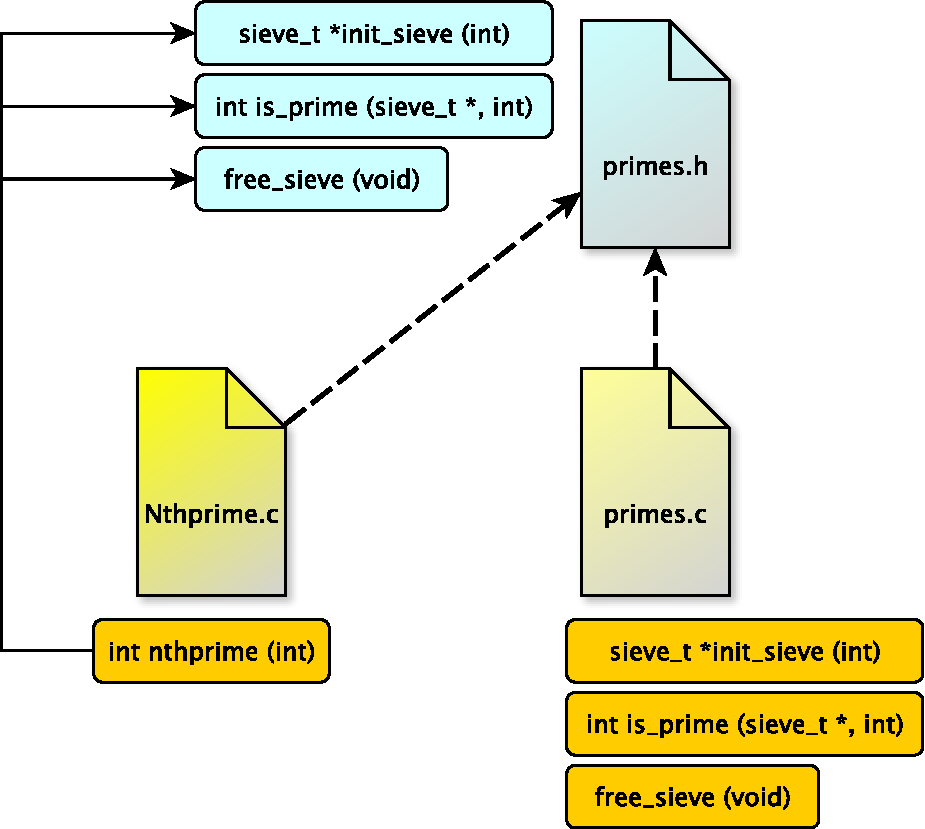
\includegraphics[width=0.8\textwidth]{illustrations/module-structure-crop.pdf}
\caption{Модульная структура программы}
\label{fig:module_struct}
\end{figure}

Если модуль primes.c достаточно стабилен, нет нужды каждый раз перекомпилировать его. Достаточно один раз скомпилировать его в специальный формат библиотечного файла -- libprimes.a или libprimes.so после чего подключать к линкеру опцией -lprimes. Но это уже платформенно-специфично, в windows речь идёт о DLL, в Linux может потребоваться PIC-код для so-модулей, etc. Всё это выходит за рамки курса, но достаточно легко осваивается по мануалам к вашей системе.

\textbf{Вопрос к студентам:} так ли нужны h-файлы? Что если непосредственно написать объявление \lstinline!init_sieve! в точке использования и предоставить линкеру самому найти тело этой функции.

\ifanswers
Правильный ответ: формально да, так можно сделать. Но реально единые заголовочники помогают бороться с человеческими ошибками. Когда изменяются типы параметров в точке определения, компилятор подскажет несоответствие заголовочнику и все места где их надо изменить в точке использования. Если же заголовочника не будет а программист забудет это сделать, будет тихое UB
\fi

\textbf{Домашняя наработка:} попробовать слинковать libprimes как статическую и как динамическую библиотеку и подключить к компиляции

\subsection{Дьяволы деталей синтаксиса C}\label{DevilDetails}

\hfill\textit{Probably the oddest aspect of C}

\hfill\textit{is the declaration syntax}{\vspace{0.5em}}

\hfill\textit{-- Dennis Ritchie}

В эпиграф вынесены (с некоторым сокращением) слова создателя языка C, сказанные им в интервью журналу C++ Report в 2000-м году, после нескольких десятков лет торжественного шествия языка по миру. И, в общем, человек знал что говорил. Пусть стоит задача прочитать простое объявление на языке C

% \lstinputlisting[firstline=5,lastline=5]{cpp_code/p1s1.cpp}
\begin{lstlisting}
char *ap[20];
\end{lstlisting}

\textbf{Вопрос к студентам:} что это? 

\ifanswers
Ответ: да, это массив указателей\index{Array of pointers}. 
\fi

\textbf{Вопрос к студентам:} как правильно написать указатель на массив?

\ifanswers
Ответ\index{Pointer to array}:

\begin{lstlisting}
char (*pa)[20];
\end{lstlisting}
\fi

Теперь рассмотрим модификатор \lstinline!const!\index{const}. 

\textbf{Вопрос к студентам:} есть ли разница между следующими объявлениями:

\begin{lstlisting}
const int *xc1;
int const *xc2;
int * const xc3 = 0;
\end{lstlisting}

\ifanswers
Ответ: между первым и вторым нет, между вторым и третьим очень существенная разница. Во втором случае (как и в первом) речь идёт о \textbf{не константном} указателе на константные данные. В третьем случае речь идёт о \textbf{константном} указателе на не константные данные. Объявляя константу нельзя оставить её неинициализированной, поэтому инициализатор выделяет строчку, где объявлен константный указатель. В то же время, указатель на константные данные сам может быть неконстантным и инициализации не требует (хотя она возможна).
\fi

\textbf{Вопрос к студентам:} как правильно написать константный указатель на константные данные? Сделать это надо двумя способами, не меньше.

\textbf{Вопрос к студентам:} что значит ключевое слово \lstinline!volatile!\index{volatile}, каковы способы его использования?

\textbf{Вопрос к студентам:} Запишите теперь константый указатель на волатильные данные. Имеет ли он смысл? Можете ли вы представить ситуацию, когда вам может понадобиться волатильный указатель на константные данные?

\ifanswers
Ответы на первые два вопроса очевидны, но ответ на третий может быть несколько экзотичен: если этот указатель \lstinline!register! переменная, которая определяет область памяти откуда идёт чтение и которая при этом соответсвует не настоящему регистру а некоему устройству, притворяющемуся регистром, но допускающему смену состояний, то конструкция обретает смысл.
\fi

Кроме того константность и волатильность также могут комбинироваться. Скажем возможен \lstinline!const volatile! указатель на \lstinline!const volatile! данные. В стандарте и прочих нормативных документах константность и волатильность любят объединять под общим названием ``cv\-qualifier''\index{cv-qualifier} (C++14 3.9.3). Далее также будет употребляться термин ``cv\-квалифи\-цированный тип'', это значит тип, к которому (возможно) добавлена константность, волатильность или обе сразу.

\textbf{Вопрос к студентам:} чем отличается \lstinline!const volatile int! от \lstinline!const int!?

\ifanswers
Правильный ответ: константность означает, что оттуда можно только читать. При этом волатильность означает, что чтения оттуда нельзя переупорядочивать. Интересно, что здесь \lstinline!const! это по сути способ сказать \lstinline!readonly!, чем семантически выразить неизменность данных.
\fi

\subsection{Чтение объявлений, как источник радости\index{C declarations}}\label{AlgDecl}

\textbf{Вопрос к студентам:} прочитайте объявление:

\begin{lstlisting}
char* const *(*next)();
\end{lstlisting}

\ifanswers
Правильный ответ: указатель на функцию, возвращающую указатель на константный указатель на символ.
\fi

Алгоритм чтения таких объявлений (приведён например в \cite{linden}) следует из стандарта и в данном случае довольно прост:

\begin{itemize}
\item
Идём к имени переменной ``next''
\item
Группируем её с содержимым её скобок: ``next is a pointer to''
\item
За пределами скобок объявление функции имеет больший приоритет, поэтому ``next is a pointer to a function, returning''
\item
Далее обрабатываем слева звёздочку, имеем: ``next is a pointer to a function, returning pointer to''
\item
И далее парсим char * const: ``next is a pointer to a function, returning pointer to constant pointer to character''
\end{itemize}

В почти алгоритмическом виде, он изображен на рисунке (\ref{fig:cdecl_parse}). Также многие любят пользоваться специальными онлайн-приложениями, такими как \url{cdecl.org}.

\begin{figure}[h!]
\centering
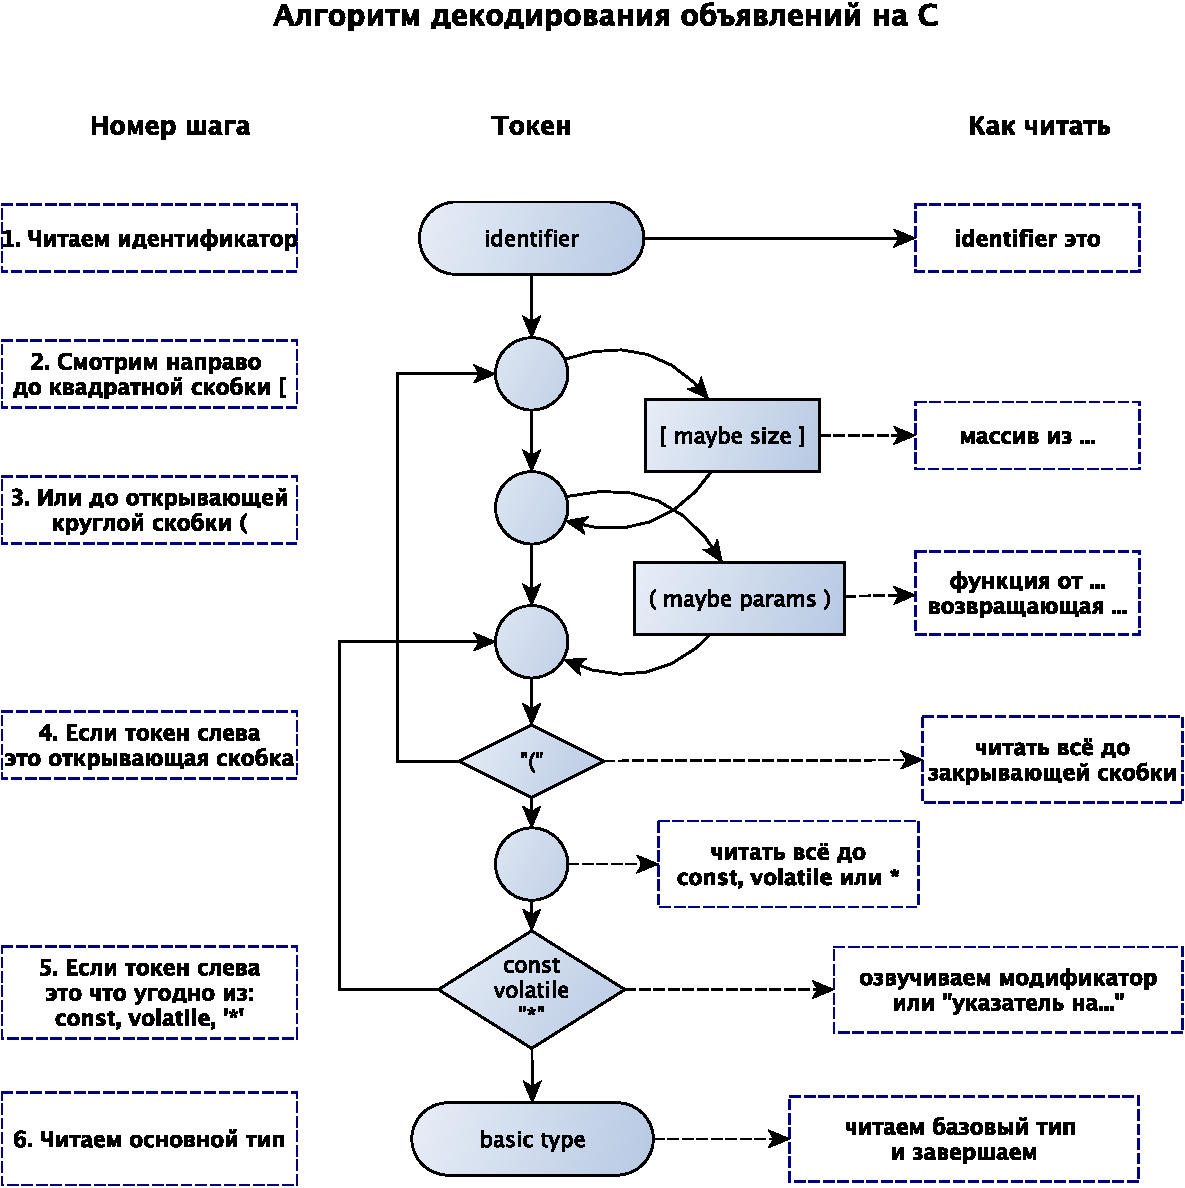
\includegraphics[width=1.0\textwidth]{illustrations/cdecls-crop.pdf}
\caption{Алгоритм разбора объявлений на C}
\label{fig:cdecl_parse}
\end{figure}

\textbf{Домашняя наработка:} по этому алгоритму написать программу, которая парсила бы произвольное объявление на C. Также учесть возможность \lstinline!enum!, \lstinline!struct!, \lstinline!union!.

\textbf{Вопрос к студентам:} с учетом новых знаний, прочитать самостоятельно

\begin{lstlisting}
char *(*c[10])(int **p);
\end{lstlisting}

\ifanswers
Ответ: c is array of 10 pointers to functions, accepting pointer to pointer to int and returning pointer to char.
\fi

\subsection{Ваш друг typedef\index{typedef}}\label{FriendTypedef}

Рассмотрим прекрасное объявление типа:

\begin{lstlisting}
void (*signal(int sig, void (*func)(int)) ) (int);
\end{lstlisting}

С помощью \lstinline!typedef! его можно переписать, доставив гораздо меньше боли глазам читающего (и без риска посадить случайную опечатку).

\begin{lstlisting}
typedef void (*ptr_to_func) (int);
ptr_to_func signal(int, ptr_to_func);
\end{lstlisting}

Умение читать запутанные объявление не означает необходимости их писать (если вы не участвуете в международном конкурсе по обфускации программ). Где возможно, следует использовать \lstinline!typedef!, это хороший стиль. Но хороший личный стиль (с другой стороны) это не основание не иметь навыка чтения запутанных объявлений. Каждый программист в жизни имеет дело с тоннами унаследованного кода, где встречается всякое.

У \lstinline!typedef! есть некоторые опасности, которые часто ускользают от новичков. Так например \lstinline!typedef! может объявить сразу несколько синонимов типов:

\begin{lstlisting}
typedef int *ptr, (*fun)(), arr[5];
\end{lstlisting}

Это считается дурным тоном, старайтесь этого избегать. Ещё более дурным тоном считается зарыть typedef вглубь объявления, что тоже позволяется синтаксисом.

\begin{lstlisting}
unsigned const long typedef int volatile *kumquat;
\end{lstlisting}

Опытный программист на языке C часто чувствует себя свободнее с препроцессором, скажем вместо

\begin{lstlisting}
typedef int * int_ptr;
\end{lstlisting}

Есть соблазн написать

\begin{lstlisting}
#define INT_PTR int *
\end{lstlisting}

Но здесь есть тонкая ловушка:

\begin{lstlisting}
INT_PTR x, y; /* x is pointer, y is int */
int_ptr w, v; /* w, v are pointers */
\end{lstlisting}

Здесь переменные \lstinline!x! и \lstinline!y! будут разных типов, а \lstinline!w! и \lstinline!v! – одного типа.

Первое и основное отличие языка C++ от языка C заключается в том, что в C++, благодаря развитой системе типов, препроцессор нужен гораздо реже и гораздо меньше.

\subsection{Мелкие шероховатости}\label{LittleDivergences}

C-подмножество языка C++ лишено некоторых возможностей, к которым мог быть привычен программист на C. Здесь они вкратце освещаются.

\begin{itemize}
\item
Функция \lstinline!main()! в C++ не может быть вызвана из пользовательского кода. В языке C это разрешено, хотя и несколько необычно.
\item
Прототипы функций обязательны в C++, но опциональны в C.
\item
Сложная и развитая система инициализации в C обычно не работает в C++

\begin{lstlisting}
struct T {
    union {
        struct {
            int x, y, z;
        };
        int xyz[3];
    };
    int a;
};

struct T v = { { .x = 1, .y = 2, .z = 3}, 4 };
struct T w = { { .xyz[0] = 1, .xyz[1] = 2, .xyz[2] = 3}, 4 };
struct T x[] = { [0].a = 1, [1].a = 2 };
\end{lstlisting}

Такой код инициализации легален в C и совершенно нелегален в C++
\item
Имена, определяемые через \lstinline!typedef! не могут совпадать с существующими именами структур в C++, но могут в C (последний требует явной квалификации \lstinline!struct!).
\item
При присвоении к \lstinline!void *! указателю указателя на иной тип, C++ требует приведения (C не требует, но оно считается хорошим тоном).
\item
C++ вводит более десяти новых ключевых слов. Они могут быть использованы как идентификаторы в программе на C, но компилятор C++ выдаст ошибку.
\item
В языке C++ объявление переменной может появится везде, где может быть выражение; в C, объявления должны быть в начале блока.
\item
Имя структуры или объединения во внутренней области видимости скроет такое же имя любой переменной во внешней области видимости в C++, но не в C.
\item
У символьных литералов тип char в C++, но тип int в C. То есть \lstinline!sizeof('a')! даёт 1 в C++, но может дать большее значение в C.
\end{itemize}

\pagebreak
\section{Борьба с препроцессором}

\hfill\textit{Almost every macro demonstrates}

\hfill\textit{a flaw in the programming language,}

\hfill\textit{in the program, or in the programmer.}{\vspace{0.5em}}

\hfill\textit{-- Bjarne Stroustrup}

Пример с \lstinline!typedef! показывает, что использование возможностей языка лучше, чем использование препроцессора. Есть целый ряд возможностей, которые кардинально отличают даже базовое подмножество C++ от чистого C и использование которых является хорошим тоном. Но есть и случаи, когда обойтись без препроцессора сложно.

\subsection{От макросов к константам времени компиляции}\label{ConstVsDef}

C-стилем в программировании является использование всюду препроцессора:

\begin{lstlisting}
#define BITS_PER_BYTE 8
#define sieve_type_bytes sizeof(sieve_type)
#define sieve_type_bits (sieve_type_bytes * BITS_PER_BYTE)
#define max_bit (1U << (sieve_type_bits - 1))
\end{lstlisting}

У такого подхода есть ряд недостатков: нет явного указания и контроля типов, происходит текстовая подстановка, в результате имена ``портятся'' для применения в программе, не пишется отладочной информации об именах констант и так далее.

В противоположность этому C++ подход состоит в явном задании хорошо типизированных констант:

\begin{lstlisting}
const unsigned BITS_PER_BYTE = 8;
const unsigned sieve_type_bytes = sizeof(sieve_type);
const unsigned sieve_type_bits = sieve_type_bytes * BITS_PER_BYTE;
sieve_type max_bit = (1U << (sieve_type_bits - 1));
\end{lstlisting}

Удивительно, что этот код не является корректным кодом на языке C, потому что в C одни константы не могут использоваться для инициализации других констант.

Ещё в большей степени это касается работы с перечислениями (строго говоря, она и в C была введена только в C99).

\begin{lstlisting}
/* C-style */
#define kword_TOKEN 10
#define kword_LITERAL 30
#define kword_SPACE 40
/* C++-style */
enum keyword {TOKEN = 10, LITERAL = 30, SPACE = 40};
\end{lstlisting}

Здесь кроме очевидной экономии места, вводится тип keyword, который может принимать только определённые в enum значения, что также является преимуществом.

\textbf{Вопрос к студентам:} видите ли вы какие-нибудь проблемы с таким подходом?

\ifanswers
Возможный ответ: да, символьное имя \lstinline!TOKEN! может конфликтовать с другим перечислением.
\fi

Кроме того, было бы очень хорошо иметь возможность в цикле пройти по всем элементам перечисления (сейчас это сложно, так как они не обязаны занимать не только последовательные, но даже и просто регулярно расположенные номера).

Более подробно эти проблемы и варианты их решения будут изложены несколько позже (см. \ref{EnumClass})

\subsection{Внешние, статические и встраиваемые функции}\label{Inline}

Любой идентификатор (переменная, функция) введенный в программе может иметь внешнее или внутреннее связывание (linkage). При разговоре о структуре программ (\ref{ProgramStructure}) уже было упомянуто, что линкер может найти функцию из одного модуля, объявленную в другом модуле. Но если бы это было верно для всех функций, две функции с одинаковыми именами не могли бы существовать в пределах всех единиц трансляции. 

К счастью, в C и в C++ функция может быть объявлена имеющей внутреннее связывание (модификатор \lstinline!static!), что означает, что она не экспортируется из модуля а используется только внутри него. Для указания внешнего связывания можно использовать ключевое слово \lstinline!extern! но вообще-то оно считается для функций указанным по умолчанию.

Обратите внимание: ключевое слово \lstinline!static! для переменной в глобальном диапазоне и внутри функции означает разные вещи. В глобальном диапазоне это ключевое слово означает внутреннее связывание, а внутри функции -- статическую переменную (то есть сохраняющую значение между вызовами функции).

Кроме внутреннего связывания, C и C++ поддерживают для функций (но не для переменных!) спецификатор \lstinline!inline!, обозначающий, что функция рекомендуется для встраивания: то есть вместо настоящего вызова, её тело будет размещено в точке вызова. Важно понимать, что использование ключевого слова \lstinline!inline! это не приказ, а совет, оно увеличивает шансы на подстановку но не обязует компилятор её производить.

\textbf{Вопрос к студентам:} если компилятор может не подставлять функцию, обозначенную как \lstinline!inline! и может подставить функцию не обозначенную таким образом, зачем вообще писать этот модификатор?

\ifanswers
Возможный ответ: \lstinline!inline! позволяет определение функции в каждом модуле (но увы это можно парировать тем, что для этого есть \lstinline!static!)
\fi

Правильный ответ: возможности компиляторов для встраивания как правило ограничены, так как слишком большой размер модулей это тоже плохо. Поэтому крайне часта ситуация, когда стоит выбор между несколькими функциями, каждую из которых можно встроить, но не все вместе. В этих случаях \lstinline!inline! помогает компилятору расставить приоритеты.

Благодаря встраиванию, C++ сильно выигрывает для определения небольших функций, где в C были выгодны макросы. Хороший пример -- вычисление максимума двух чисел.

Типичный контекст использования

\begin{lstlisting}
int a = 5, b = 0;
assert (MAX(a,b) == 5);
\end{lstlisting}

Вариант реализации на C:

\begin{lstlisting}
#define MAX(a, b) ((a) > (b) ? (a) : (b))
\end{lstlisting}

Вариант реализации на C++:

\begin{lstlisting}
static inline long
MAX (long a, long b)
{
  return (a > b) ? a : b;
} 
\end{lstlisting}

Оба эти варианта работают для тривиальных случаев. Ниже приведён чуть более сложный код, для которого начинаются проблемы.

\begin{lstlisting}
int a = 5, b = 0;
int c = MAX(++a, b);
int d = MAX(++a, b+10);
\end{lstlisting}

\textbf{Вопрос к студентам:} что будет содержаться в \lstinline!c! и в \lstinline!d!? А что если подставить вызов функции \lstinline!max!? 

\ifanswers
Правильный ответ: макрос раскроется как \lstinline!((++a) > (b) ? (++a) : (b))! то есть в сишной версии \lstinline!a! будет инкрементирована дважды. В C++ версии всё норм.
\fi

Пока что сишный вариант, тем не менее, обладает некоторой притягательностью: если исключить сайд-эффекты, то во-первых он является безразличным относительно типов аргументов (type generic), так что его можно использовать и для \lstinline!double! в то время, как плюсовый вариант как он сейчас написан, требует только чисел типа \lstinline!long!. В (\ref{FunctionTemplate}) будут рассмотрены средства, которые позволяют написать обобщенный максимум на C++

Есть ещё аргумент относительно штрафа на производительность из-за вызова функции. Но поскольку вызов \lstinline!max! почти всегда будет проинлайнен, эффективность C++ метода как минимум не страдает. Более того, почти всегда, когда в C использовался \lstinline!void*! для передачи параметров неопределённого типа, в C++ можно написать более эффективный код, используя шаблоны. Подробный разбор этого следует несколько отложить (см. \ref{FunctionTemplate}).

Удивительно, но даже без встраивания функций, замена макросов на функции может дать прирост производительности

\begin{lstlisting}
#define SQR(x) ((x)*(x))
unsigned sqr (x) { return x*x; }
\end{lstlisting}

в контексте использования

\begin{lstlisting}
unsigned t = SQR(f(x));
\end{lstlisting}

Если в квадрат возводится результат вычисления функции \lstinline!f!, то вариант с макросом вызовет её дважды, а вариант с функцией вызовет её один раз.

Модификатор \lstinline!inline! появился и в языке C (начиная с C99) но там он работает по другим правилам: функция, объявленная \lstinline!inline! по умолчанию считается не \lstinline!static! а \lstinline!extern!. Внешние встраиваемые функции означают, что в каждом модуле вы должны предоставить тело такой функции для возможного встраивания, но, если встраивания не произойдёт, будет вызвана та из них, где \lstinline!extern! указан явно.

На C++ \lstinline!extern inline! тоже можно писать, но тут правила гораздо мягче: стандарт всего лишь требует от линкера выбрать какую-то одну реализацию чтобы сгенерировать из неё тело для вызова (C++14 7.2.1).

\textbf{Вопрос к студентам:} в чём по-вашему может быть смысл писать \lstinline!extern inline! функции?

\ifanswers
Возможный ответ: разница кроется в семантике статических переменных. Внутри \lstinline!static inline! функций создается столько их копий сколько функций, внутри \lstinline!extern inline! копия одна на всех.
\fi

\subsection{Когда нужен препроцессор}\label{subsub:preprocuses}

В некоторых случаях препроцессор всё-таки нужен. Так, например, в (\ref{ProgramStructure}) был описан случай включения заголовочных файлов с использованием \lstinline!#include!. Возможно в стандарте C++20 пройдет предложение по модулям в языке и тогда эта практика станет устаревшей, но пока это единственная (и хорошо проверенная временем) возможность организовать модульность.

Также почти всегда нужны так называемые стражи включения, позволяющие избежать включения одного и того же модуля дважды. Например в ситуации когда в процессе включения возникает циркулярная ссылка, они бывают полезны чтобы прервать её. Но и вообще простановка стражей включения это хороший тон, так что реальный модуль primes.h из (\ref{ProgramStructure}) будет выглядеть как-то так:

\begin{lstlisting}
#ifndef PRIMES_GUARD_
#define PRIMES_GUARD_

/* ... something meaningfull ... */

#endif
\end{lstlisting}

Ещё один случай это отключение неиспользуемого кода по опции сборки

\begin{lstlisting}
#ifndef VERBOSE
#define VERBOSE 0
#endif

#if (VERBOSE == 1)
/* ... some logging ... */
#endif
\end{lstlisting}

Эта программа скомпилированная с \lstinline!-DVERBOSE=1! будет выполнять дополнительный код, заключенный под директиву препроцессора.

Иногда нужно использовать черную магию препроцессора, например возможности по конкатенации:

\begin{lstlisting}
struct command
{
  char *name;
  void (*function) ();
};
     
struct command commands[] =
{
  { "quit", quit_command },
  { "help", help_command },
  /* ..... */
};
\end{lstlisting}

Гораздо яснее и проще

\begin{lstlisting}
#define COMMAND(NAME)  { #NAME, NAME ## _command }
     
struct command commands[] =
{
  COMMAND (quit),
  COMMAND (help),
  /* ..... */
};
\end{lstlisting}

Это уберегает от человеческих ошибок (скажем несоответствия имени хендлеру), но использование таких конструкций должно быть исключением, а не правилом.

Иногда применение препроцессора связано с необходимостью трюков для применения по косвенности:

\textbf{Вопрос к студентам:} что ниже следует поставить, чтобы добиться искажения функции по значению переменной:

\begin{lstlisting}
#define VARIABLE 3

/* ... some magic? ... */

extern void NAME(mine)(char *x);
/* creates mine_3 function */
\end{lstlisting}

\ifanswers
Правильный ответ должен включать не менее трёх уровней косвенности:

\begin{lstlisting}
#define PASTER(x,y) x ## _ ## y
#define EVALUATOR(x,y)  PASTER(x,y)
#define NAME(fun) EVALUATOR(fun, VARIABLE)
\end{lstlisting}

Порядок расширения макросов следующий:

\begin{lstlisting}
NAME(mine)
EVALUATOR(mine, VARIABLE)
PASTER(mine, 3)
\end{lstlisting}

Поэтому пропустить хотя бы один уровень косвенности здесь нельзя.
\fi

При использовании препроцессора важном понимать, что он работает в один проход.

\begin{lstlisting}
#define h_h # ## #
#define mkstr(a) # a
#define betw(a) mkstr(a)
#define join(c, d) betw(c h_h d)
char p[] = join(x, y);
cout << p << endl;
\end{lstlisting}

\textbf{Вопрос студентам:} что на экране?

\ifanswers
Порядок расширения следующий:

\begin{lstlisting}
join(x, y)
betw(x # ## # y)
mkstr(x ## y)
"x ## y"
\end{lstlisting}
\fi

Ответ в общем очевиден: на экране \lstinline!"x ## y"! причём символ \lstinline!##! получился после конкатенации двух символов хеша \lstinline!# ## #!.

Допустим, теперь мы хотим, чтобы эта конкатенация исполнилась до превращения в строку и на экране было \lstinline!"xy"!. Здесь добавление лишнего уровня косвенности уже не поможет. Увы, увы, препроцессор не начинает проверку на возможную идентификацию аргументов для свежеобразованных токенов. Именно поэтому, к слову, он не Тьюринг полон. Тьюринг-полный, мощный и правильный препроцессор называется GNU M4 (https://www.gnu.org/software/m4/m4.html) но, если честно, он мало кем всерьёз используется.

\textbf{Домашняя наработка:} в качестве упражнения написать свой многопроходный препроцессор. 

Все рассмотренные в этом разделе случаи полезного использования препроцессора, касаются, как можно заметить, его базового применения: обработки текста программы. Во всех остальных случаях при программировании на C++ использования препроцессора стараются избегать.

\pagebreak
\section{Базовые концепции языка}\label{BasicTerms}

Есть существенное отличие между знанием как работает язык и знанием почему он так работает. Стандарты языков и руководства по программированию часто написаны в очень разных терминах. В основе C++ лежит целая совокупность фундаментальных понятий: точки объявления и инстанцирования, полные и неполные типы, правые и левые ссылки, области видимости и спецификаторы связывания. Все они крайне важны. В этом разделе будет рассмотрено некоторое количество таких корневых концепций, без которых дальнейшее понимание языка будет затруднено.

\subsection{Объявления и определения\index{declaration}\index{definition}}\label{DeclVsDef}

До сих пор действия с объявлениями и определениями выполнялись интуитивно, без полного понимания того, что это такое. Настало время обратить внимание на детали.

Объявление (declaration) это введение идентификатора и описание типа.

\begin{lstlisting}
extern int bar;
extern int g(int, int);
double f(int, double); // extern can be omitted for function declarations
class foo;             // no extern allowed for class declarations
\end{lstlisting}

Нужно обратить внимание на перегруженный смысл ключевого слова \lstinline!extern! в этом контексте. В (\ref{Inline}) оно использовалось для задания внешнего/внутреннего связывания, тогда как здесь используется оно же, но для указания, что переменная объявлена, но не определена.

Объявление достаточно компилятору, чтобы разрешить ссылки на данный идентификатор. 

Определение (definition) это реализация типа или выделение памяти объекту.

\begin{lstlisting}
int bar;
int g(int lhs, int rhs) {return lhs*rhs;}
double f(int i, double d) {return i+d;}
class foo {};
\end{lstlisting}

Определение достаточно линкеру, чтобы реализовать идентификатор в объектном коде. 

Объявление может встречаться сколько угодно раз. Определение может встретиться лишь один раз. Это называется One Definition Rule (ODR\index{ODR}) и оно должно чётко соблюдаться. Нарушение ODR -- UB. При этом любое определение также является объявлением.

У ODR есть несколько уровней строгости и из него есть несколько исключений, подробнее см. (C++14 3.2) где они перечислены.

\begin{itemize}
\item функции и переменные с внешним связыванием должны быть определены один раз на все единицы трансляции
\item встраиваемые (inline) функции, статические (static) функции и переменные, определения пользовательских типов, шаблоны классов и их частичные специализации должны быть определены не более одного раза в каждой единице трансляции
\end{itemize}

Можно запомнить мнемоническое правило чтобы не путать объявление с определением, а в англоязычной литературе declaration и definition, нужно смотреть на словарное упорядочение.  Буква ``б'' расположена по алфавиту раньше, чем ``п''. Значит в словаре слово ``объявление'' будет раньше, чем ``определение'' и так же declaration в английском словаре идёт раньше, чем definition. И так же в программе – объявление всегда должно идти раньше определения.

Не стоит путать также определение переменной и её инициализацию. Переменная может быть определена но не инициализирвоана. В C и в C++ чтение неинициализированной переменной это UB (например C99 6.3.2.1/2).

Важной концепцией является точка объявления (Point of Declaration, сокращенно PoD) \index{Point of Declaration}. Объявление имени считается законченным когда записан полный идентификатор (то есть \textbf{до} возможных инициализаторов). Поэтому:

\begin{lstlisting}
int x = 2;
{
  int x /* PoD */ = x;
}
\end{lstlisting}

В этом случае значение внутреннего \lstinline!x! не определено. Но в следующем случае:

\begin{lstlisting}
int x = 2;
{
  int x[x] /* PoD */;
}
\end{lstlisting}

всё корректно и вложенный массив имеет два элемента.

\textbf{Вопрос к студентам:} хорошо, в первом случае оно не определено. Но если программа будет, тем не менее, читать значения из такой неинициализированной переменной, будет ли каждый раз получаться одно и то же (пусть мусорное) значение или могут быть всегда разные?

\ifanswers
Ответ: могут быть всегда разные, так как UB
\fi

Интересно, что строчка одного и того же вида может служит определением или объявлением в зависимости от контекста:

\begin{lstlisting}
typedef void T();
T t; // declaration of function "t"

typedef int T;
T t; // definition of object "t"
\end{lstlisting}

Эта ассимметрия связана с (исторической) ассиметрией объявлений функций и переменных.

Также при определении не должен сужаться объявленный linkage specifier, поэтому вот так можно:

\begin{lstlisting}
static int x;
extern int x; // x still static
\end{lstlisting}

А вот так нельзя:

\begin{lstlisting}
extern int x;
static int x; // compilation error
\end{lstlisting}

Во втором случае storage class переменной уже заявлен как внешний и не может быть переопределен.

Больше про объявления и определения классов в (\ref{DeclDefs}).

\subsection{Область видимости и время жизни}\label{ScopeLifeTime}

С концепцией точки объявления, связана концепция области видимости. Область видимости \index{Scope} переменной, объявленной внутри блока из фигурных скобок это текст программы от точки определения до закрывающей фигурной скобки блока. В стандарте можно посмотреть правила для других областей видимости (C++14 3.3).

Гораздо более интересной концепцией является время жизни переменной. Время жизни переменной бывает не равно её области видимости.

Область видимости (scope) это те места в программе, где возможно обращение к переменной.

Время жизни (lifetime) это все то время, когда возможно \textbf{корректное} обращение к переменной.

Чтобы не сравнивать время с пространством, можно также сказать, что кроме области в которой переменная видима, есть область в которой она валидна. Но иногда такое упрощение искажает смысл, так что лучше им не пользоваться.

Для автоматических и нелокальных статических переменных, их время жизни почти всегда совпадает с временем выполнения программы, проведённом в их области видимости.

\textbf{Вопрос к студентам:} охарактеризуйте следующий код:

\begin{lstlisting}
int foo(int x) {
  int y, *p;

  {
    int z = 5; 
    p = &z;
  }

  y = *p;
  return y;
}
\end{lstlisting}

\ifanswers
Правильный ответ: этот код демонстрирует undefined behavior. В точке разыменования указателя истекло время жизни того, на что он указывает.
\fi

\textbf{Вопрос к студентам:} теперь охарактеризуйте следующий код:

\begin{lstlisting}
int foo(int x) {
  int y, *p;

  {
    static int z = 5; 
    p = &z;
  }

  y = *p;
  return y;
}
\end{lstlisting}

\ifanswers
Правильный ответ: здесь работает ещё одна перегруженная функция ключевого слова \lstinline!static! -- оно расширяет время жизни переменной до времени жизни программы. Таким образом здесь будет все хорошо -- переменная \lstinline!z! будет жить даже между вызовами функции.
\fi

Вещи становятся сложнее, когда в игру вступает динамическая память:

\begin{lstlisting}
int* f (int n) {
  int *p = malloc (sizeof(int) * n); /* 1 */
  return p;
} /* 2 */

int main () {
  int *q = f (10); 
  free (q); /* 3 */
}
\end{lstlisting}

Здесь область видимости переменной \lstinline!p! заканчивается в точке 2, а время жизни объекта в динамической памяти -- в точке 3.

С указателями все ещё интереснее: оказывается само время жизни указателя зависит от жизни объекта, на который он указывает. Стандарт регламентирует (C99 6.4.2), что ``The value of a pointer becomes indeterminate when the object it points to reaches the end of its lifetime''. Например:

\begin{lstlisting}
int *p = malloc (sizeof(int));
long pold = (long) p;
free (p);
assert (p == (int *)pold); /* ORLY? */
\end{lstlisting}

Здесь время жизни \lstinline!p! закончилось, хотя \lstinline!p! это локальная переменная и она не выходила из области видимости.

На самом деле, время жизни оканчивает не только \lstinline!free! но и \lstinline!realloc!. Известный технический анекдот основан на так называемом ``N. Lewycky realloc'' (реаллок Левицкого). Ник Левицкий, инженер LLVM compiler team предложил следующий код

\begin{lstlisting}
int *p = malloc (sizeof(int));
int *q = realloc (p, sizeof(int));
*p = 1;
*q = 2;
if (p == q)
  printf ("%d %d\n", *p, *q);
\end{lstlisting}

И на тогдашнем clang, этот код распечатал ему ``1 2'', что, вообще говоря, безумие, потому что получается, что в программе есть два одинаковых указателя, которые указывают на разные объекты.

Конечно здесь UB из-за использования указателя после \lstinline!realloc! т.е. после окончания времени жизни.

\subsection{Полные и неполные типы}

Если тип (структура, класс, массив) только объявлен, но не определен то этот тип считается неполным. Полным тип становится только в точке, в которой встречается его определение. Но даже неполного типа вполне хватает для объявлений. На примере структур:

\begin{lstlisting}
struct t; /* declare type t */

extern int foo(t p); /* ok, incomplete function type */
extern t x; /* ok, incomplete variable */
extern t arr[]; /* ok, incomplete array */
\end{lstlisting}

\textbf{Вопрос к студентам:} можно ли написать определение для объекта неполного типа?

\ifanswers
Правильный ответ: конечно нет, так как неизвестно сколько памяти надо такому объекту. Но можно написать определение указателя на такой объект.
\fi

\subsection{Lvalue и rvalue\index{lvalue}\index{rvalue}}\label{LRvalues}

Следующий пример, многим может показаться излишне простым.

\begin{lstlisting}
x = y;
\end{lstlisting}

Что здесь написано? Здесь написано – взять адрес переменной \lstinline!x! и записать по этому адресу значение переменной y. В этом выражении присваивания, переменная \lstinline!x! находится в выражении слева, а \lstinline!y! -- справа и стандарт C++98 вводит специальные термины rvalue (right-hand-side value) и lvalue (left-hand-side value) интуитивно понимаемые как ``нечто, что может быть справа (слева) в выражении присваивания'' (C++98 3.10). 

Итак, какие ограничения этот пример накладывает на \lstinline!x!? Похоже, что \lstinline!x! должен быть полного типа, не константым, и иметь определённое местоположение в памяти (быть адресуемым). Есть ли ограничения на \lstinline!y!? Да есть. Он должен быть полного типа и этот тип должен быть совместим с типом \lstinline!x! по присваиванию.  

Это типичный пример того, как компилятор может решить из контекста (в данном случае из положения справа или слева от присваивания) будет ли он использовать адрес переменной или её значение в своих фактических вычислениях. Такая возможность у компилятора есть, потому что адрес переменной полного типа всегда известен во время компиляции и нет необходимости заставлять программиста его специально получать.

\begin{lstlisting}
*(&x) = y;
\end{lstlisting}

Возможно, кстати, писать так было бы честнее.

Стандарт C++11 существенно расширяет и дополняет классификацию категорий значений, речь об этом пойдет в (\ref{LRvaluesAgain}).

\pagebreak
\section{Массивы и указатели}\label{subsec:arrpointers}

\hfill\textit{Should array indices start at 0 or 1?}

\hfill\textit{My compromise of 0.5 was rejected without,} 

\hfill\textit{I thought, proper consideration}{\vspace{0.5em}}

\hfill\textit{-- Stan Kelly-Bootle}

Многие программисты заучивают правило для новичка: массивы в C это указатели и наоборот. Это правило, пожалуй, действительно полезно для новичка. Но в общем случае это не так. В этом разделе будут проведены чёткие разграничения. 

\subsection{Вспоминаем указатели}

Указатель хранит адрес, по которому программа может прочитать и (в случае неконстантных данных) записать значение, того типа, из которого выведен тип указателя. Для любой переменной на протяжении её времени жизни (\ref{ScopeLifeTime}) стандарт гарантирует побитовую неизменность адреса (C11 6.2.4).

С неконстантным указателем можно сделать следующее:

\begin{enumerate}
\item Объявить и инициализировать константой
\begin{lstlisting}
int *x = 0;
\end{lstlisting}
\item Объявить и инициализировать адресом переменной или функции
\begin{lstlisting}
struct str_t {int x; int y;};
int foo (int x);
int c = 2;
str_t s = {1, 2};
int *p = &c;
int (*pfoo) (int) = &foo;
str_t *ps = &s;
\end{lstlisting}
\item Присвоить иное значение
\begin{lstlisting}
int bar (int x);
p = x;
x = &c;
pfoo = &bar
\end{lstlisting}
\item Разыменовать и получить или изменить значение
\begin{lstlisting}
c = *x;
*p = 5;
c = (*ps).x;
c = ps->x;
ps->x = *p;
\end{lstlisting}
\item Использовать индексацию, похожую на массив
\begin{lstlisting}
p[0] = c;
*(p+0) = c;
\end{lstlisting}
\item Возвращать из функций
\begin{lstlisting}
int *foo (int x) { return &x; }
\end{lstlisting}
\end{enumerate}

Неконстантные указатели являются lvalue. В принципе, можно записать:

\begin{lstlisting}
  int p = 3;
  int *pp = (int *) p;
  return *pp;
\end{lstlisting}

Этот код является дурным тоном, он будет плохо переносим и совершенно точно тут указатель используется не по назначению, но важно, что это можно сделать. Указатель это честная ячейка памяти. Он хранит то, что туда положил программист, как это показано на рисунке \ref{fig:pointers}.

\begin{figure}[h!]
\centering
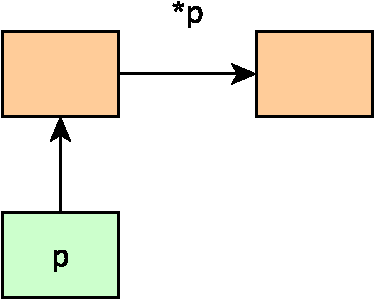
\includegraphics[width=0.3\textwidth]{illustrations/pointers-crop.pdf}
\caption{Визуальное представление указателей}
\label{fig:pointers}
\end{figure}

\textbf{Вопрос к студентам:} можно ли сериализовать указатели, например в файл, а потом восстанавливать и использовать?

\ifanswers
Ответ: да, в течении срока жизни того, на что они указывают.
\fi

\textbf{Вопрос к студентам:} можно ли для переменной сказать сколько указателей на неё в данный момент существует?

\ifanswers
Ответ: увы, нет. Никакая переменная не ``знает'' о том, что кто-то взял её адрес и т.п.
\fi

Это, вообще говоря, сильно снижает возможности компиляторов к оптимизации.

\begin{lstlisting}
float *b; 
int x;
// ...... (etc)
x = 1;
*b = 5;
x = x + 3;
foo (x);
\end{lstlisting}

Этот код мог бы быть оптимизирован как показано ниже

\begin{lstlisting}
x = 4;
*b = 5.0;
foo (4);
\end{lstlisting}

Но компилятор не имеет права этого делать: в строчках кода помеченных троеточием вполне могло встретится нечто вроде утечки адреса с конвертацией типа

\begin{lstlisting}
b = (float *) &x;
\end{lstlisting}

И в этом случае запись \lstinline!*b = 5.0! непредсказуемо изменит \lstinline!x!.

В связи с этим, сообществом и большинство компиляторов (но не стандартом) поддерживаются \textbf{strict aliasing rules}\index{strict aliasing}\label{StrictAliasing}. Их суть -- в запрещении доступа к данным одного типа по указателю другого типа. Большинство компиляторов проверяют strict aliasing по умолчанию и требуют специальных опция для его отключения.

Кроме того, в стандарте языка C99 (но не C++) для указателей поддерживается модификатор \lstinline!restrict! (C99 6.7.3)

\begin{lstlisting}
void f (int n, int * restrict p, int * restrict q){
  while (n-- > 0)
  *p++ = *q++;
}
\end{lstlisting}

Здесь программист как бы дает компилятору обещание, что на вход \lstinline!f! придут непересекающиеся области данных.

\subsection{Арифметика указателей}

Кроме всего прочего, указатели можно складывать с целыми числами, а также вычитать из них целые числа и указатели друг из друга.

Для сложения, указателем может быть любой из операндов (но только один из них, сложить два указателя нельзя). Для вычитания обязательно левый операнд должен быть указателем, а правый -- указателем или числом

\begin{lstlisting}
int arr[] = {0, 1, 2, 3, 4, 5};
int a = 0; 
int *b = &arr[0];
int *c = b + a;      // ok
int *d = a + b;      // ok
int *e = c + d;      // ok
ptrdiff_t f = c - d; // ok
int *g = c - a;      // ok
int *h = a - c;      // error
\end{lstlisting}

Следует обратить внимание на тип \lstinline!ptrdiff_t! в коде выше -- это специальный тип, достаточно широкий, чтобы хранить разность указателей. Следует по возможности пользоваться им, но, как запасной вариант, есть тип \lstinline!long! (которого увы не хватает для LLP64 систем, таких как Win64, но он вполне пригоден для почти всех unix-специфичных приложений). Он находится в хедере \lstinline!<stddef.h>!.

\textbf{Вопрос к студентам:} как вы думаете возможно ли посчитать разницу между указателями на стеке и в куче?

\begin{lstlisting}
int *t = malloc (sizeof(int));
int k = 4;
ptrdiff_t d = t - &k; /* ok? */
\end{lstlisting}

\ifanswers
Правильный ответ: разумеется да, адресная арифметика по стандарту прозрачна относительно того где расположена память до тех пор, пока все влезает в \lstinline!ptrdiff_t!.
\fi

\subsection{Нулевые указатели}\label{NullPointers}

Особой разновидностью указателей являются нулевые указатели. Их смысл -- сигнализировать об отсутствии указуемого значения, будь то конце строки, завершение односвязного списка или не выделенная ещё память. Первое, что нужно о них запомнить: нулевой указатель может быть не нулевым. В этом смысле константы \lstinline!0!, \lstinline!NULL! или, скажем, \lstinline!nullptr! из нового стандарта это разные константы. Для конкретной архитектуры значение \lstinline!NULL! может быть \lstinline!0xffff0000!, или любым другим.

Но во всех распространенных архитектурах \lstinline!NULL == 0! и чтобы сохранить обратную совместимость существующего кода, стандарт определяет правила неявной конверсии \lstinline!0! в \lstinline!NULL! при сравнении с ним указателей (C99 6.3.2.3).

\begin{lstlisting}
int *t = malloc(sizeof(int));
assert(t); // ok, means assert(t != NULL)
\end{lstlisting}

Здесь условие под \lstinline!assert! будет неявно сконвертировано в правильную форму. Конечно, программист, заботящийся о стиле, сразу пишет правильно:

\begin{lstlisting}
int *t = malloc (sizeof(int));
assert (t != NULL); // great 
\end{lstlisting}

Но и в первом варианте нет ошибки.

\textbf{Вопрос к студентам:} но ведь ноль может быть не только вбит, но и предвычислен:

\begin{lstlisting}
int *zerop = (int*)(x – y);
assert (zerop == NULL);
\end{lstlisting}

Представим, что в этом случае \lstinline!NULL == 0xffff0000! и при этом \lstinline!x == y!. Сработает ли assertion?

\ifanswers
Правильный ответ: увы, нет. Стандарт гарантирует стабильное обращение с нулями времени компиляции, но не нулями времени исполнения (C99 6.3.2.3), иначе проверками пришлось бы завешивать слишком много кода.
\fi

\subsection{Действия с массивами}

Встроенные массивы (также C-массивы) исторически предшествовали указателям и представляют собой простейший вид синтаксического клея -- логически непрерывную область памяти, побитую на однотипные ячейки.

С массивами также возможны некоторые действия.

\begin{enumerate}
\item Объявить и инициализировать списком данных (все пропущенные инициализаторы -- нулевые)
\begin{lstlisting}
int a = 5;
int x[10] = {6, a};
\end{lstlisting}

Следует обратить внимание: неинициализированным может быть только локальный массив. Глобальные массивы всегда инициализированы нулями.

Также следует обратить внимание. Определение вида:
\begin{lstlisting}
int wrong[]; /* boom! */
\end{lstlisting}
Это ошибка (поскольку компилятор не знает сколько памяти выделять на этот массив). Но можно использовать такой синтаксис в объявлениях
\begin{lstlisting}
extern int wrong[]; /* ok */
\end{lstlisting}
\item Прочитать или записать значение
\begin{lstlisting}
int t = x[0];
x[1] = t;
x[0] = x[1];
\end{lstlisting}
\item Деградировать (decay) к указателю если он используется как rvalue\label{ArrDecaying}\index{Decay}
\begin{lstlisting}
int foo (int *t);
int *p = &x[0];
*p = x;          // decay
a = *(x + 3);    // decay 
a = foo (x + 5); // decay 
\end{lstlisting}
\end{enumerate}

\begin{figure}[h!]
\centering
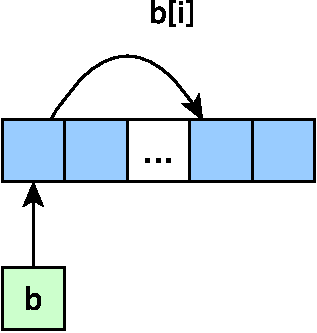
\includegraphics[width=0.3\textwidth]{illustrations/arrays-crop.pdf}
\caption{Визуальное представление массивов}
\label{fig:arrays-crop}
\end{figure}

Но массивы \textbf{никогда} не употребляются вместо указателей там, где указатель это lvalue.

\begin{lstlisting}
int v = 5;
int *p = &v;
int a[1] = {v};
p = a; // oks
a = p; // never
\end{lstlisting}

По той же причине нет возможности вернуть массив из функции:

\begin{lstlisting}
typedef int arr_t[10];

arr_t foo (); // Error!
\end{lstlisting}

Разумеется, невозможна никакая арифметика массивов -- прибавить один массив к другому или вычесть один массив из другого в языке C невозможно.

Массивы хранят сами данные, а не указатели на них. То, что они синтаксически могут вырождаться к указателям -- удобная концепция, связанная с ранней историей массивов в языке C и в дальнейшем получившая неожиданно глубокое и мощное развитие в последних версиях стандарта C++ (см. \ref{Decaying}). Массив содержит lvalue-ячейки данных, но сам как целое он не является lvalue-ячейкой данных.

\subsection{Инициализация массивов и указателей}

Инициализация массивов и указателей выглядит похоже, но означает разные вещи:

\begin{lstlisting}
char a[] = "abcdefgh";
char *b = "abcdefgh";
assert (a[3] == b[3]);
\end{lstlisting}

\textbf{Вопрос к студентам:} есть ли разница между этими двумя записями и какую вы предпочтёте? Почему?

\ifanswers
Верный ответ: строчка 1 предпочтительней, чем (устаревшая, с Wall + Werror выдаст ``error: deprecated conversion from string constant to \lstinline!char*!'') строчка 2 и они имеют разную семантику. Память под массивы выделяется автоматически (и строчка 1 подразумевает неявный memset) но память никогда автоматически не выделяется под указатели, поэтому для построения динамических структур данных (например, связных списков) используются указатели, а не массивы.
\fi

Между прочим, строковые литералы в инициализации указателей это счастливое (исторически сложившееся) исключение. Строчка 2 в следующем примере не будет скомпилирована:

\begin{lstlisting}
float a[] = {1.0, 2.0, 3.0}; // ok
float *b = {1.0, 2.0, 3.0};  // ka-boom!
\end{lstlisting}

\textbf{Вопрос к студентам:} есть ли разница между следующими двумя объявлениями?

\begin{lstlisting}
int foo(int x[]);
int foo(int *x);
\end{lstlisting}

\ifanswers
Ответ: из-за decaying разницы нет.
\fi

\textbf{Вопрос к студентам:} означает ли эта запись:

\begin{lstlisting}
int foo(int x[16]);
\end{lstlisting}

что \lstinline!foo! принимает массив из 16 символов?

\ifanswers
Ответ: нет, здесь \lstinline!foo! принимает любой указатель.
\fi

\subsection{Прогулки за границами}\label{subsub:overruns}

Хорошо написанный код никогда не должен ничего считывать и записывать за границами массивов. В общем случае проблема доступа к данным вне выделенного для доступа буфера называется ``buffer overflow'' или ``buffer underflow'' и является (не только в C) одним из основных источников уязвимостей программ. Увы, такие языки как C имеют к нему родовую предрасположенность: максимальная эффективность требует отсутствия неявных проверок времени выполнения.

К чему это приводит можно проиллюстрировать на примере простейшей уязвимости:

\begin{lstlisting}
char buff[16];
int pass = 0;

printf("\n Enter the password : \n");
gets(buff);

if (strcmp (buff, "correctpassword")) {
  printf ("\n Wrong Password \n");
}
else {
  printf ("\n Correct Password \n");
  pass = 1;
}

if (pass) {
  // Now Give root or admin rights to user
  printf ("\n Root privileges given to the user \n");
}
\end{lstlisting}

Здесь чтобы демонстрация была эффектной придется скомпилировать без оптимизаций чтобы переменная попала на стек:

\begin{verbatim}
$ g++ p1-overrun.cpp -O0 -m32
$ ./a.out
Enter the password : 
hhhhhhhhhhhhhhhhh

 Wrong Password 

 Root privileges given to the user 
\end{verbatim}

Введен очевидно неверный пароль. Но, поскольку он переполняет стек, последний символ записывается в переменную \lstinline!pass! и таким образом её значение меняется и пароль засчитывается как верный.

Это самый простой, можно сказать ``детский'' пример такой уязвимости, в реальности всё сложнее и разнообразнее, но идея именно эта.

Частично защититься от порчи стека в GCC может помочь опция \lstinline!-fstack-protector-all! -- с ней программа просто упадет, оставив трассу

\begin{verbatim}
$ g++ p1-overrun.cpp -O0 -m32 -fstack-protector-all
$ ./a.out 

 Enter the password : 
hhhhhhhhhhhhhhhhh

 Wrong Password 
*** stack smashing detected ***: ./a.out terminated
\end{verbatim}

Если вы используете другой компилятор, у него скорее всего существуют аналогичные средства, кроме того существует целый класс бесплатных и коммерческих программ (их хорошо искать по ключевым словам bounds checking).

Эти программы, конечно, тоже не панацея. В большинстве они отлавливают только уже произошедшую запись в неправильное место на стеке, реально же проблемы с уходом за границу массива могут быть гораздо более тонкими и даже вообще не включать порчи стека. Например по стандарту арифметика указателей в пределах массива не должна уходить дальше, чем на один элемент от границ массива:

\begin{lstlisting}
int arr[] = {0, 1, 2, 3, 4, 5};
int *a = arr;   // ok, decaying as &arr[0]
int *b = a + 3; // ok, *b == 3
int *c = a + 6; // ok, c is one past arr
int *d = a + 7; // undefined behavior
d = d - 4;      // even here, *d is undefined
\end{lstlisting}

Пятая строчка здесь создает UB и весь код поcле этой строчки теряет предсказуемость. Даже если программа, ничего не меняя за границами массива, ``честно'' возвращается в допустимую область, тем не менее, UB уже случилось, жесткий диск уже отформатирован, всё пропало.

\subsection{Многомерные массивы\index{multidimensional arrays}}\label{MultiDimArr}

Настоящий многомерный массив (вообще -- настоящий массив) это абстрактный тип данных \lstinline!A!, для которого определены две операции \lstinline!get(A, I)! и \lstinline!set(A, I, V)!. При этом выполняются аксиомы:

$get(set(A,I,V),I)=V$

$get(set(A,I,V),J)=get(A,J)|I \neq J$

В качестве индекса служит кортеж произвольных объектов, обычно целых чисел.

Язык C и C-подмножество языка C++ не поддерживают семантику многомерного массива на уровне языка.

Хуже того, существует противоречие между статическими многомерными массивами (которые на самом деле одномерные с хитрым доступом) как на (рис. \ref{fig:c_arrays}) и динамическими многомерными массивами (там же).

\begin{figure}[h!]
\centering
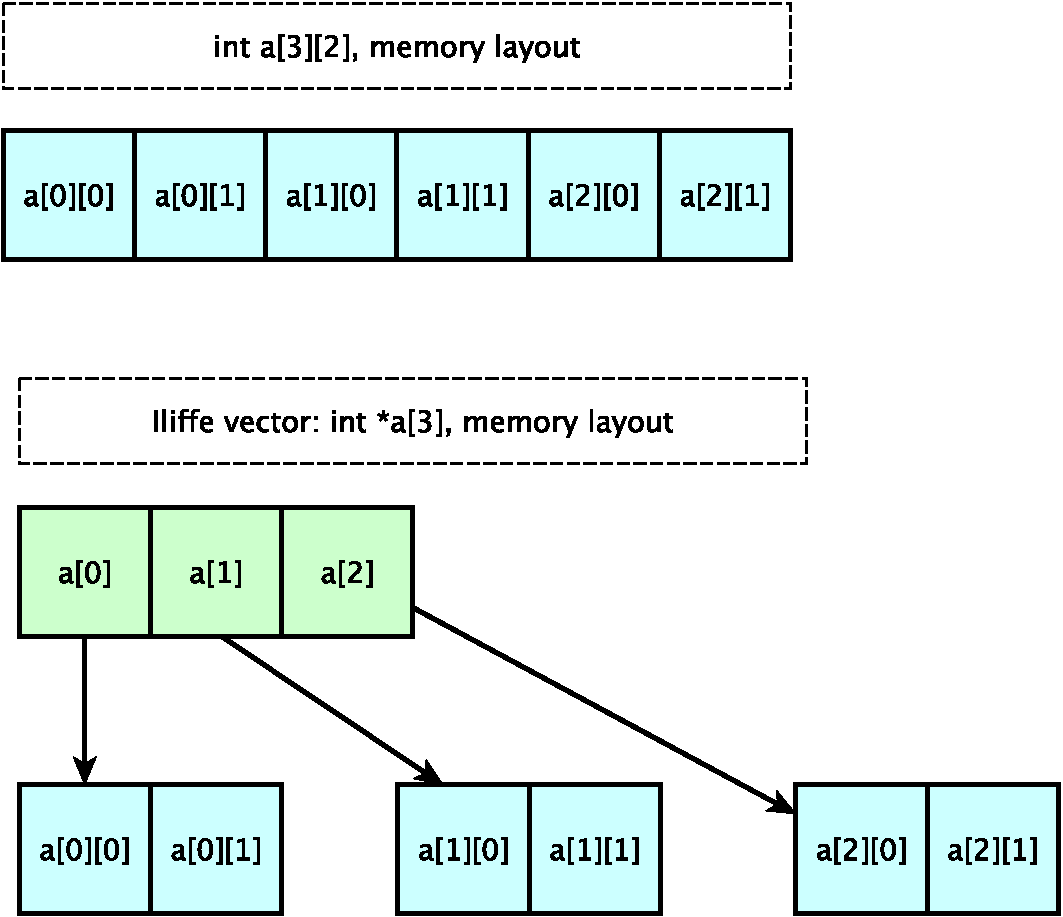
\includegraphics[width=0.8\textwidth]{illustrations/arraylayout-crop.pdf}
\caption{Массивы в языке C}
\label{fig:c_arrays}
\end{figure}

Из-за этого в точке обращения к массиву существует контекстная зависимость -- неясно обращение к чему именно происходит: к jagged-вектору или к одномерному статическому массиву с двумерной адресацией?

\begin{lstlisting}
assert(a[3][4] == *(a + 3*jmax + 4); // option 1
assert(a[3][4] == *(*(a + 3) + 4);   // option 2 
\end{lstlisting}

Статические массивы в памяти должны всегда быть непрерывны. Для многомерных массивов раскладка в памяти идёт построчно (см. рис. \ref{fig:c_arrays}). При этом последние индексы идут последними. Так же и с инициализацией.

\begin{lstlisting}
float flt[][3] = {{1.0, 2.0, 3.0}, {4.0, 5.0}}; // ok
\end{lstlisting}

При этом наиболее вложенные скобки относятся к последним индексам. Первый индекс ясен из контекста и его можно опускать в инициализаторе.

Если часть вложенных инициализаторов пропущена, они считаются нулевыми, поэтому, например двумерные массивы символов могут быть проинициализированы последовательностями строковых литералов.

При передаче многомерных массивов в функции может быть опущен только первый индекс в прототипе (и он может быть любым). Остальные индексы у формального и фактического аргументов должны совпадать.

\textbf{Вопрос к студентам:} возможен ли такой прототип функции?

\begin{lstlisting}
int func(int a[][], int n);
\end{lstlisting}

\ifanswers
Правильный ответ: нет, так как у статического массива не могут быть опущены оба индекса. Допустимы следующие варианты:

\begin{lstlisting}
int func(int a[][3], int n);
int func(int (*a)[3], int n);
\end{lstlisting}
\fi

Точно так же нельзя, даже указав нужные инициализаторы, определить двумерный массив, для которого компилятор дедуцирует оба размера

\begin{lstlisting}
int a[][] = {{1, 2}, {3, 4}}; // Error!
\end{lstlisting}

Увы, но здесь, как и в прототипах функций, должны быть указаны все размеры, кроме, может быть, первого.

\textbf{Вопрос к студентам:} в функцию можно передать массив вместо указателя. Можно ли передать двойной массив туда, где ожидается двойной указатель?

\begin{lstlisting}
int func(int **a, int n, int m);
int a[2][3];
func (a, 2, 3); // huh?
\end{lstlisting}

\ifanswers
Но это не работает. Двумерный массив уже не может деградировать к указателю на указатель, а только к указателю на массив (из рисунка \ref{fig:c_arrays} причины должны быть уже очевидны). 
\fi

\textbf{Вопрос к студентам:} есть ли возможность передать двойной массив туда, где ожидается одинарный указатель?

\ifanswers
Ответ: да, есть забавный трюк.

\begin{lstlisting}
int func(int *a, int n, int m);
int a[2][3];
func (&a[0][0], 2, 3); /* ok */
\end{lstlisting}

Но внутри функции это потребует ручного обслуживания такого ``развернутого'' массива.
\fi

\pagebreak
\section{От указателей к ссылкам\index{references}}\label{PointersAndRefs}

Очень важной особенностью C++ является введение довольно низкоуровневой, но принципиально новой конструкции – ссылок. Ссылка это альтернативное имя переменной.

\begin{lstlisting}
int x = 5;
int &xref = x;
xref += 1;
assert(x == 6);
\end{lstlisting}

Каждая ссылка обязательно должна быть инициализирована в точке определения. ``Ссылка сама по себе'' так же как ``нулевая ссылка'' не могут существовать. Указатель сам по себе является местом для хранения данных, ссылка – это просто имя. Поэтому ссылки не нуждаются в явном разыменовании – каждое обращение к ним это уже разыменование. Поэтому различия существенны:

\begin{lstlisting}
int x[2] = {10, 20};
int &xref = x[0];
int *xptr = &x[0];
xref += 1;
xptr += 1;
assert((xref == 11) && (*xptr == 20));
\end{lstlisting}

\subsection{Использование ссылок}

Главный паттерн для использования ссылок это передача по ссылке входных (неизменяемых) аргументов функций, особенно если типы являются жирными:

\begin{lstlisting}
struct T {
  // a lot of content here
};

int foo(const T &a);
\end{lstlisting}

Здесь можно использовать и указатель, но тогда в теле функции его придется постоянно разыменовывать, проверять на \lstinline!NULL! и так далее. Ссылка в этом отношении удобней, прозрачней и безопасней.

С другой стороны, передача изменяемых параметров по неконстантным ссылкам -- дело вкуса:

\begin{lstlisting}
int do_r (T &a);
int do_p (T *a); // maybe a is array?

do_r (b); // should b be changed?
do_p (&b);
\end{lstlisting}

Некоторые считают, что это создаёт неоднозначность в точке использования. Другие считают, что указатели также создают неоднозначность между массивом и указателем.

Не стоит передавать по ссылкам небольшие объекты. У подрастающих программистов часто чешется написать нечто вроде:

\begin{lstlisting}
int foo(const int &a);
\end{lstlisting}

Это допустимо, но тут лучше передать \lstinline!a! по значению. Внутри компилятора ссылки обычно реализуются через указатели, которые могут превосходить по размеру небольшие целые. Поэтому тут ваш выбор:

\begin{lstlisting}
int foo(int a);
\end{lstlisting}

Просто и понятно.

Ещё один паттерн использования ссылок -- задание временных имён для безымянных объектов:

\begin{lstlisting}
int &current = big_global_array[calc_index(t)];
current += 1; // ok, big_global_array changed
\end{lstlisting}

В этом деле ссылки настолько удобны, потому что по стандарту они продлевают время жизни автоматических переменных:

\begin{lstlisting}
const int &c = a + foo();
use (c); // ok, c holds temporary value
\end{lstlisting}

В противовес этому использование в этом контексте указателя создало бы UB.

Здесь связывание константной ссылки (const reference binding) продляет время жизни временного объекта. Обратите внимание: ссылка связана с временным объектом. При попытке использовать там неконстантную ссылку ничего работать не будет. Зато константная ссылка продляет всё что угодно, даже константу

\begin{lstlisting}
const int &lv = 0; // ok
\end{lstlisting}

Теперь \lstinline!lv! это второе имя для нуля.

\textbf{Вопрос к студентам:} как вы думаете, можно ли вычислить адрес временного объекта на который ссылается \lstinline!lv!?

\ifanswers
Ответ: увы нет и, более того, сам этот объект не обязан существовать.
\fi

Ссылки дают важную возможность наконец-то передавать в функцию встроенные массивы фиксированного размера с контролем длины

\begin{lstlisting}
int foo(int arr[3]); // really: int *arr
int bar(int (&arr)[3]); // ok, ref to arr

int wrong[5];
foo(wrong); // ok
bar(wrong); // fail
\end{lstlisting}

Без ссылок у нас была только псевдо-возможность указать размер (ну и конечно перегрузка ключевого слова static в языке C для статического хинта такого рода, но вот об ЭТОМ лучше сразу забыть).

\subsection{Висячие ссылки}\label{DanglingRefs}

Итак, ссылка это второе имя объекта. Но что если срок жизни объекта истёк?

\begin{lstlisting}
int *t = malloc (sizeof (int) * 10);
int &r = t[2];
free (t); /* end of lifetime */
use (r); /* BOOM */ 
\end{lstlisting}

В этом случае ссылка считается ``повисшей'' (dangling\index{dangling reference}) и любое её использование это UB.

Аналогично ссылка может повиснуть если возвращать из функции ссылку на временный объект. Последние версии современных компиляторов выдают на эту тему предупреждение, но закладываться на это не стоит.

\begin{lstlisting}
int& refret (int x) {
  return x;
}

int &v = refret (3);
printf ("%d\n", v); /* BOOM */
\end{lstlisting}

Здесь тоже всё очень плохо.

\textbf{Вопрос к студентам:} как исправить приведенный выше код и всё-таки вернуть валидную ссылку из функции?

\ifanswers
Ответов может быть много: статические переменные, динамическая аллокация, глобалы, выберите ваш вариант
\fi

\textbf{Вопрос к студентам:} что можно сказать насчёт возврата временного объекта в ссылку по значению?

\begin{lstlisting}
int xret (int x) {
  return x;
}

const int &lv = xret (1);
\end{lstlisting}

\ifanswers
Правильный ответ: тут всё нормально, работает обсуждавшееся выше расширение срока жизни.
\fi

\subsection{Когда ссылки уступают указателям}\label{PointersVsRefs}

В целом при программировании на C++ следует повсюду предпочитать использование ссылок использованию указателей.

Но есть нюансы. Ссылки иммутабельны -- назначив ссылку ``другим именем'' чего-то, её нельзя перевязать на что-то другое

\begin{lstlisting}
int a = 2;
int b = 3;

int *pa = &a;
pa = &b;      // ok, now pa == &b

int &ra = a;
ra = b;       // ok, now a == 3, ra still means a
\end{lstlisting}

Вторая строчка в случае ссылок -- не перевязывает ссылку, а присваивает значение тому lvalue на которое она ссылается. Поэтому ссылки нельзя использовать для создания динамических структур данных, таких как стеки, очереди, деревья.

Кроме того, у ссылок нет аналога \lstinline!(void *)! для передачи идиомы ``ссылки на неопределённый тип''. Появившиеся в новом стандарте \lstinline!auto&! всё таки должны быть разрешены на этапе компиляции, что бывает невозможно:

\begin{lstlisting}
void *read ();

// using somewhere below

int a = *(int *) read(); // read int
double d = *(double *) read(); // next read double
\end{lstlisting}

\textbf{Домашняя наработка} найдите другие случаи, в которых использование ссылок невозможно или нецелесообразно.

\pagebreak
\section{Искажение имён и его последствия\index{Function Overloading}\index{Name Mangling}}\label{NameResolution}

\hfill\textit{If names be not correct, language is not in accordance}

\hfill\textit{with the truth of things}{\vspace{0.5em}}

\hfill\textit{-- Confucius}

Язык C предоставляет достаточно сильную гарантию того, что любое имя, использованное в вашей программе будет уникально связано с типом, областью видимости и так далее.

Обычно это приводит к тому, что имя отображается в ассемблер целевой машины один к одному, без искажения или с несущественным искажением (скажем к stdcall именам под Windows добавляется подчеркивание в начале, то есть \lstinline!foo! станет в ассемблере \lstinline!_foo!).

Язык C++ такой гарантии не даёт. Вместо этого он согласен сделать работу по созданию уникальных имён (и многую другую работу) за программиста посредством встроенного искажения (манглирования) имён. 

\subsection{Манглирование и перегрузка}\label{subsub:mangling}

\textbf{Вопрос к студентам:} сколько функций вычисления квадратного корня вы можете назвать из стандартной библиотеки языка C?

Правильный ответ: три (7.12.7.5) \lstinline!sqrtf!, \lstinline!sqrt! и \lstinline!sqrtl!. Три функции с разными именами понадобилось вводить потому, что они принимают аргументы разных типов.

Используя C++ вы можете написать три функции с одинаковыми именами, но различными типами:

\begin{lstlisting}
char bar (char x) { return x; }
int bar (int y) { return y; }
long long bar (long long z) { return z; }
\end{lstlisting}

На уровне ассемблера они могут выглядеть например так:

\begin{verbatim}
_Z3barc:
....
_Z3bari:
....
_Z3barx:
....
\end{verbatim}

Конвенции манглирования не документированы и являются зависимыми от реализации, так что закладываться на них не надо. Но грамотно использовать механизм перегрузки функций в C++ бывает очень выгодно для облегчения читаемости вашей программы.

Для большинства компиляторов C++ существуют ``деманглеры'' -- специальные приложения, способные по искаженному имени ассемблерной метки восстанавливать сигнатуру функции. Скажем в GCC это \lstinline!c++filt!. Попробуйте, скажем: \lstinline!c++filt _ZN4Anls3Cfg7_DeleteEPKv!

Искажение имён позволяет больше, чем перегрузку. По сути, все средства абстракции C++, включая ООП и шаблоны возможны в этом языке только благодаря наличию в нём искажения имён. В этом разделе рассматривается только применение в перегрузках, про искажение имён методов структур см. (\ref{CCppStructs}).

Иногда требуется из кода на C++ сделать некую функцию или переменную (обычно входящую в интерфейс модуля) ``линкуемой в C стиле'' -- т.е. отображаемой в ассемблер один в один. Для этого используется спецификатор линковки \lstinline!extern "C"!. Им можно как аннотировать функцию или переменную, так и брать их в блоки.

\begin{lstlisting}
extern "C" void foo(int);

extern "C" {
  void g(char);
  int i;
}
\end{lstlisting}

Так слинкованы могут быть свободные функции и глобальные переменные, но не члены классов. Две функции с такой линковкой с одинаковым именем -- нарушение ODR.

\textbf{Домашняя наработка:} посмотрите как работает манглирование в вашем любимом компиляторе. Можете ли вы установить некие закономерности?

Функция не может быть перегружена по: 

\begin{itemize}
\item Имени аргумента
\item Типу возвращаемого значения
\end{itemize}

Кроме того, функции не могут быть перегружены по cv-квалификаторам

\begin{lstlisting}
void foo (int);
void foo (const int); // FAIL

void bar (char *);
void bar (char * const); // FAIL
\end{lstlisting}

Однако это не относится к cv-квалификаторам самого внешнего типа

\begin{lstlisting}
void foo (int&);
void foo (const int&); // OK

void foo (char *);
void foo (const char *); // OK
\end{lstlisting}

Перегрузка даёт серьёзные преимущества по сравнению с языком C. В частности, она позволяет решать некоторые вопросы более естественно. Как пример можно рассмотреть функцию \lstinline!strchr!. В стандартной библиотеке C++ она задана двумя перегрузками

\begin{lstlisting}
const char * strchr (const char * str, int c);
      char * strchr (      char * str, int c);
\end{lstlisting}

Здесь смысл совершенно ясен: если мы ищем символ в константной строке, то и позиция будет в константной строке и наоборот.

В языке C перегрузка невозможна, и, поэтому, там сделано куда более опасно

\begin{lstlisting}
char * strchr (const char * str, int c); // C version
\end{lstlisting}

Здесь есть гипотетическая возможность вызвать \lstinline!strchr! для констатной строки и вернуть неконстантный указатель, изменение по которому ведёт к UB, поэтому за этим надо постоянно следить, чтобы так не сделать. Это неудобно, опасно и хрупко.

Но кроме положительных сторон и приятных удобств, в перегрузке есть и тонкие и неприятные моменты. Например правила её разрешения.

\subsection{Правила разрешения перегрузки\index{overloading resolution}}\label{Overloading}

После того, как компилятор составил множество функций-кандидатов на разрешение перегрузки (viable set) исключив все, которые кандидатами быть не могут, разрешение происходит в следующем порядке.

\begin{enumerate}
\item Идеальное совпадение (включая правильный ссылочный тип)
\item Стандартные преобразования
\item Пользовательские преобразования
\item Троеточия
\item Ссылочное связывание (для неправильных ссылок)
\end{enumerate}

После каждого типа преобразований сверху-вниз, получается множество возможных функций. Если это множество состоит из одной функции, будет вызвана она. Если это множество состоит из нескольких функций, будет выдана ошибка компиляции. Если это множество пусто, будет попробован следующий тип преобразований аргументов.

Предположим, в пользовательском коде стоит вызов

\begin{lstlisting}
foo(10);
\end{lstlisting}

А чуть ранее объявлены следующие функции:

\begin{lstlisting}
int foo(char x) { return 0;}        // 1
int foo(short x) { return 1;}       // 2
int foo(int x) { return 2;}         // 3
int foo(...) { return 3;}           // 4
int foo(int &x) { return 4;}        // 5
int foo(const int &x) { return 5;}  // 6
\end{lstlisting}

При таком множестве перегрузки, вызов не скомпилируется, поскольку здесь есть конфликт между (3) и (6), которые подходят одинаково хорошо.

Если стереть (6), то никаких конфликтов не остаётся. Для вызова \lstinline!foo (10)! точно подходит только \lstinline!foo(int)! и программа возвращает 2.

Если теперь стереть (3), то будет ошибка компиляции:

\begin{lstlisting}
int foo(char x) { return 0;}        // 1
int foo(short x) { return 1;}       // 2
int foo(...) { return 3;}           // 4
int foo(int &x) { return 4;}        // 5
\end{lstlisting}

Конфликт между двумя равноправными функциями (1) и (2), обе работают через один шаг стандартных преобразований. Если далее стереть одну из них, например (2) всё снова становится норм, программа вернёт 0. Если стереть оставшуюся функцию (1), то следующей пойдёт (4).

Если убрать всё и оставить только (5), то будет ошибка компиляции: функция \lstinline!foo! выиграет перегрузку, но константа не может быть связана с неконстантной lvalue ссылкой. Зато такое ссылочное связывание засчитывается как точное совпадение если вызов происходит для lvalue.

\begin{lstlisting}
void foo(int x); // 1
void foo(int &x); // 2
void foo(const int &x); // 3

int x = 42;
foo(x); // (1, 2) or (1, 3) -> conflict 
        // (2, 3) -> (2) 
\end{lstlisting}

Если вдуматься в эти правила они уже не выглядят столь марсианскими, правда? Хех. Это от того, что я рассказал вам их \textbf{не все}. На уровне C подмножества, всё выглядит довольно логично, но вы уже сейчас можете заглянуть в перегрузку с учётом шаблонов (см. \ref{TemplOverloading})

Начиная с C++11, перегрузки можно стирать, используя ключевое слово \lstinline!delete!

\begin{lstlisting}
// for int
int foo (int number);

// not for char or bool
int foo(bool) = delete;
int foo(char) = delete;
\end{lstlisting}

Такой синтаксис запрещает перегрузку с заданными типами аргументов. Тем не менее, эти функции участвуют в перегрузке, поэтому при точном совпадении

\begin{lstlisting}
foo(true); // error, not foo(int)
\end{lstlisting}

будет именно ошибка компиляции, вместо неявного приведения типа.

Перегрузка функций это очень общий механизм, к нему ещё предстоит вернуться неоднократно.

\subsection{Аргументы по умолчанию}\label{subsub:defaultagrs}

Отсутствия обязательств C++ быть близким к машине позволяет ещё более удивительные вещи, такие как аргументы по умолчанию. Это значения аргументов функции (всегда в конце списка аргументов), которые не обязаны быть указаны при вызове

\begin{lstlisting}
char foo(char x = 0);
int bar(int x, int y = 5);
long buz(long x, long y = 5, long z = 0xafff);
\end{lstlisting}

При вызове параметры по умолчанию могут быть теперь опущены

\begin{lstlisting}
foo(); // OK, x = 0
foo('a'); // OK, x = 'a'
buz(3, 6); // OK, x = 3, y = 6, z = 0xafff
\end{lstlisting}

Аргументы по умолчанию не входят в тип функции. Например они запрещены в указателях на функции. В терминах примера выше:

\begin{lstlisting}
typedef char(*pfoo_t)(char);
pfoo_t pf = foo; // OK
pf(); // FAIL, no default arguments any more
pf('a'); // OK, foo called, x = 'a'
\end{lstlisting}

По значению аргумента по умолчанию функция также не может быть перегружена (по тем же причинам -- он не входит в тип).

Параметры по умолчанию могут быть добавлены в функцию при последующих переопределениях, но не могут быть далее изменены.

\begin{lstlisting}
char foo(char x);
char foo(char x = 0); // OK, adding default
char foo(char x = 1); // FAIL, default can not be changed
\end{lstlisting}

В качестве параметров по умолчанию могут быть использованы глобальные переменные и даже вызовы функций

\begin{lstlisting}
int a = 1;
int f(int x);
int bar(int x, int y = f(a));
\end{lstlisting}

Теперь в программе можно изменять глобальную переменную и в качестве параметра по умолчанию \lstinline!bar! будет подхвачено её значение.

\subsection{Структуры в C и в C++}\label{CCppStructs}

В языке C структура являлась способом ввести пользовательский тип, являющийся механическим объединением разнородных данных:

\begin{lstlisting}
typedef struct pair { 
  int x; 
  int y; 
} pair_t;
\end{lstlisting}

\textbf{Вопрос к студентам:} что за странный \lstinline!typedef!, зачем он нужен?

\ifanswers
Правильный ответ: это стандартная идиома, чтобы в коде на C не писать лишний раз \lstinline!struct pair! в два слова.
\fi

Можно написать функцию, создающую обратную пару:

\begin{lstlisting}
pair_t transpose_pair(const pair_t *pthis) {
  pair_t pr = {pthis->y, pthis->x};
  return pr;
} 
\end{lstlisting}

\textbf{Вопрос к студентам:} обоснована ли здесь передача по указателю?

\ifanswers
Правильный ответ: на грани. Указатель может занимать больше места, чем два целых, может и меньше.
\fi

Вызвать эту функцию тоже несложно:

\begin{lstlisting}
pair_t p = {2, 3};
pair_t t = transpose_pair (&p);
assert ((p.x == t.y) && (p.y == t.x));
\end{lstlisting}

Такие типы возможны и в C++. Но в C++ была также добавлена принципиально новая возможность группировать данные с методами их обработки внутри структуры.

\begin{lstlisting}
struct pair_t { 
  int x; 
  int y;
  pair_t transpose_pair (); 
};

pair_t pair_t::transpose_pair () {
  pair_t pr = {this->y, this->x};
  return pr;
} 
\end{lstlisting}

Из кода выше, в том числе, видно, что в C++ была исключена необходимость добавлять \lstinline!struct! к символьному имени структуры, что делает ненужным оставшийся в C-style коде \lstinline!typedef! тэга структуры на её имя.

Вызов будет выглядеть чуть иначе:

\begin{lstlisting}
pair_t p = {2, 3};
pair_t t = p.transpose_pair ();
assert ((p.x == t.y) && (p.y == t.x));
\end{lstlisting}

Это работает за счёт искажения имён (см. \ref{NameResolution}). В итоговом ассемблере имена \lstinline!transpose_pair! и \lstinline!pair_t::transpose_pair! будут разными и у вызывающего кода не будет проблем с тем, что именно он вызывает. В итоговом ассемблере, имя метода встретится, например, в виде:

\begin{verbatim}
_Z14transpose_pair4pair:
\end{verbatim}

Определённая так функция называется функцией-членом (member function)\index{member function}, а также методом структуры. Объявление метода происходит внутри определения структуры, определение метода имеет явную квалификацию того к чему метод относится. Обратите внимание, что символ сдвоенных двоеточий такой же, как и в случае пространств имён. Он дословно означает ``пространство имён, задаваемое структурой''.

Ключевое слово \lstinline!this!\index{this} обозначает неявный (всегда первый) аргумент в методе класса и является указателем на экземпляр структуры, для которой он вызывается. Поэтому \lstinline!this->y! это поле \lstinline!p.y! при вызове \lstinline!p.transpose_pair()! но это будет уже \lstinline!t.y! при вызове \lstinline!t.transpose_pair()!

По умолчанию \lstinline!this! можно опускать, чтобы не загромождать код. Имена полей класса всё равно являются идентификаторами из наиболее охватывающего пространства имён. Поэтому следующий код является и законным и совершенно эквивалентным приведенному выше:

\begin{lstlisting}
pair_t pair_t::transpose_pair() {
  pair_t pr = {y, x};
  return pr;
} 
\end{lstlisting}

Такой подход делает появление имён \lstinline!x! и \lstinline!y! в теле метода несколько неожиданным, поэтому многие авторы книг по хорошему стилю рекомендуют выделять название полей. Саттер и Александреску \cite{sutteralexandresku} рекомендуют \lstinline!x_! и \lstinline!y_!, но на практике часто встречаются \lstinline!m_x! и \lstinline!m_y!. В общем это дело вкуса.

\textbf{Вопрос к студентам:} можно ли вызвать метод класса так, чтобы \lstinline!this! был нулевым указателем?

\ifanswers
Правильный ответ: да, через явное приведение типов. Но лучше так не делать, это UB.
\fi

\pagebreak
\section{От программирования в стиле C к программированию в стиле C++}

\hfill\textit{Most people's C programs should be indented}

\hfill\textit{six feet downward and covered with dirt}{\vspace{0.5em}}

\hfill\textit{-- Blair P. Houghton}

C++ имеет много своих идиом. Многие из них на этом этапе могут быть непонятны (зачем заменять такой хороший malloc на этот странный new?) но переход на активное использование этих идиом лучше начинать уже сейчас, а их подлинная сила откроется позже.

\subsection{От ввода-вывода через функции к потокам}\label{PrintfToCout}

Все мы знаем (а автор этих лекций так и вообще предпочитает) старые добрые функции, которые в C использовались для вывода. Здесь можно их вспомнить в предпоследний раз тихим ласковым словом. Предпоследний, потому что про ввод и выводе ещё предстоит поговорить подробно в (\ref{subsec:iostreams}) и там к старым добрым возможностям придётся вернуться ещё раз.

Главной структурой, обобщающей ввод-вывод в C является структура \lstinline!FILE! (наследие идеологии Unix, где всё считается файлом, включая такие странные вещи, как консоль или сокет). Поскольку размер этой структуры implementation defined, обычно для совместимости используется \lstinline!FILE*!. Файлы можно создавать, открывать, переоткрывать и закрывать. Количество файлов, которым может оперировать программист задаётся константой \lstinline!FOPEN_MAX! и по стандарту не может быть меньше 8, включая три стандартных файла: \lstinline!stdin!, \lstinline!stdout! и \lstinline!stderr! (первый обычно является read-only и слушает клавиатуру, вторые write-only и направлены на консоль).

Файловый ввод-вывод бывает буферизованным и не буферизованным (традиционно \lstinline!stdout! буферизован, а \lstinline!stderr! нет). Буферизованный вывод накапливает определенное количество символов и только потом выводит их в файл, таким образом уменьшая число обращений к физическим устройствам вывода. С другой стороны, при аварийном завершении программы содержимое буфера может испариться, поэтому в таких сценариях лучше использовать небуферизованный вывод.

Буферизация в свою очередь бывает полной и построчной. Скажем, \lstinline!stdout! буферизован построчно -- вывод конца строки сбрасывает буфер на физическое устройство.

Для открываемых вновь файлов, программист может установить режим буферизации через \lstinline!setvbuf! (C11 7.21.5.6) а также указать собственный буфер любого размера. Очень часто большой буфер в памяти для файла позволяет в разы ускорить работу с ним. Разумеется, в любой момент буфер может быть принудительно сброшен через \lstinline!fflush!.

Ввод и вывод в файлы в языке C бывает форматированный и не форматированный. Базовые функции неформатированного ввода и вывода это \lstinline!fputc! и \lstinline!fgetc!, позволяющие посылать в файл (читать из файла) один символ. Также к базовым относится функция \lstinline!ungetc!, позволяющая временно положить назад символ в файл, доступный на чтение. Гарантируется временное помещение назад одного символа (даже для небуферизованных файлов доступных только на чтение, какой-нибудь там клавиатуры, etc). Это позволяет при необходимости ``забыть'' считанный символ а потом считать его же ещё раз и очень полезно для лексических анализаторов. Чтобы считать таким образом строку символов нужен целый цикл и чтобы избавить от необходимости писать такие циклы, существуют функции \lstinline!fread! и \lstinline!fwrite!. 

Базовый неформатированный hello world приведен ниже.

\begin{lstlisting}
fputs("Hello, world\n", stdout);
\end{lstlisting}

Форматированный ввод и вывод -- самая интересная и спорная часть стандартного вывода. Форматировать можно как вывод в файл (\lstinline!fprintf!), так и вывод в строку (\lstinline!sprintf!). С форматированием, прошлый пример будет иметь вид.

\begin{lstlisting}
fprintf(stdout, "%s\n", "Hello, world");
\end{lstlisting}

К сожалению, такой способ вывода небезопасен относительно типов (компилятор не может проверить форматную строку на соответствие типу аргумента). Он подвержен ошибкам, скажем если передать вместо строчки адрес в памяти, то будет выведено содержимое памяти до первого нулевого символа и так далее. Более того -- нет возможности расширять набор форматных спецификаторов если захочется устроить вывод для своего класса.

В C++ все сишные функции по работе с файлами оставлены, но добавлена новая сущность -- поток ввода/вывода (stream). Эти потоки не стоит путать с потоками исполнения (threads). Поток ввода вывода это не совсем файл, но он может быть основан на файле (\lstinline!fstream!) или на строке (\lstinline!sstream!). Они используются для форматированного ввода или вывода. Стандартные потоки имеют следующее соответствие со стандартными файлами:

\begin{center}
\begin{tabular}{ | l | l | l | }
  \hline
  Тип & Файл & Поток \\ \hline
  Стандартный ввод & \lstinline!stdin! & \lstinline!std::cin! \\
  Стандартный вывод & \lstinline!stdout! & \lstinline!std::cout! \\
  Сообщения об ошибках & \lstinline!stderr! & \lstinline!std::cerr! \\
  Логирование & -- & \lstinline!std::clog! \\
  \hline
\end{tabular}
\end{center}

Неформатированный вывод осуществляется через методы потоков (о том, что такое метод см. \ref{CCppStructs}). Например вывод неформатированного Hello, world через write

\begin{lstlisting}
std::cout.write("Hello, world\n", sizeof("Hello, world\n"));
\end{lstlisting}

Форматированный вывод осуществляется через несколько странную конструкцию -- перегруженный оператор сдвига влево (ввод через сдвиг справо). Подробнее про перегрузку операторов речь пойдёт дальше (см. \ref{OperatorOverloading}). Пока что стоит отметить, что такая перегрузка операторов -- очень плохая идея (логический сдвиг не имеет отношения к выводу), но исторически устоявшаяся практика. Для форматирования вывода используются форматные модификаторы.

\begin{lstlisting}
std::cout << "Hello, world" << std::endl;
\end{lstlisting}

Точно так же ввод вывод через потоки может быть буферизован. Потоки ввода-вывода будут рассмотрены подробнее когда речь пойдет про стандартную библиотеку. Пока что может быть неясно (как и со многим в этом разделе) чем они лучше, их подлинная сила вскроется позже.

\subsection{От строк в стиле C к строкам в стиле C++}\label{subsubsec:cstrings}

Язык C++ наследует от C все возможности по работе со строками, завершающимися нулём, которыми так славен последний.

\begin{lstlisting}
char astr[] = "hello";
char bstr[15];
int alen = strlen(astr);
assert(alen == 5);
strcpy(bstr, astr);
strcat(bstr, ", world!");
int res = strcmp(astr, bstr);
assert(res < 0);
\end{lstlisting}

Этот код является одновременно кодом на C и на C++. Увы, для строк в стиле C их длина не является инвариантом. Например:

\begin{lstlisting}
int foo (const char *str, size_t len)
\end{lstlisting}

Нет никакого способа здесь сказать действительно ли \lstinline!str! это строка и действительно ли её длина это \lstinline!len! кроме одного: вызвать \lstinline!strlen! и за линейное время от длины строки убедиться в этом.

Ещё хуже, что при работе с изменяемой строкой легко может возникнуть переполнение буфера и порча памяти (см. \ref{subsub:overruns} где описаны последствия).

В C++ традиционно для работы со строками используется \lstinline!std::string!, который для своих целей не сложнее (а местами и проще), чем работа в стиле C. Например, код выше можно переписать следующим образом:

\begin{lstlisting}
string astr = "hello";
string bstr; 
bstr.reserve(15);
int alen = astr.length();
assert(alen == 5);
bstr = astr;
bstr += ", world!";
int res = astr.compare(bstr);
assert(res < 0);
\end{lstlisting}

Синтаксис \lstinline!astr.length()! и \lstinline!astr.compare(bstr)! называется вызовом метода и уже рассматривался при разговоре о структурах (см. \ref{CCppStructs}).

Да, здесь есть некий оверхед, поскольку в случае с C++ строками мы (почти) безальтернативно работаем с кучей, а в случае C строк есть возможность размещать их на стеке. Но иногда это небольшая цена за (сравнительную) безопасность и удобство работы.

Если некая функция требует старых сишных строк, класс \lstinline!string! достаточно гибок и предоставляет возможность притвориться строчкой в старом стиле для старого API

\begin{lstlisting}
int res = strcmp(astr.c_str(), bstr.c_str());
\end{lstlisting}

Разумеется, так следует только читать строки, а не записывать их. Поскольку строка поддерживает длину, запись туда разрешена только через методы строки.

Подобнее о строках разговор пойдёт далее (см. \ref{subsec:strings}).

\subsection{От макросов к шаблонным функциям}\label{FunctionTemplate}

Ранее, в разделе (\ref{Inline}) рассматривалось то преимущество, которое даёт C++ (и C начиная с C99) позволяя объявлять встраиваемые функции там, где раньше использовались макросы. Но был указан и недостаток -- отсутствие возможности передавать аргументы любого типа. На самом деле эта возможность есть. Наивный подход иллюстрируется следующим определением функции:

\begin{lstlisting}
template <typename T> inline const T
min (const T a, const T b) {
  return (a < b) ? a : b;
}
\end{lstlisting}

Говорят, что здесь определен шаблон функции. Синтаксис шаблона ясен из определения: после слова \lstinline!template! в треугольных скобках через запятую перечисляются параметры шаблона. Подробности грамматики изложены в разделе 14 стандарта C++98.

\begin{lstlisting}
template <typename T, class U, int x>
\end{lstlisting}

Здесь слово \lstinline!typename! означает параметр шаблона, задающий имя типа. По историческим причинам можно использовать \lstinline!class!, но новый стандарт поощряет использование \lstinline!typename!. Кроме того вы уже должны видеть в функции \lstinline!max()! существенный недостаток – параметры, передающиеся по значению, в случае увесистого \lstinline!T! будут неэффективны, лучше заменить их константными ссылками.

Подробно шаблонные функции рассматриваются в (\ref{FunctionTemplates}).

\subsection{От malloc и free к new и delete\index{new}\index{delete}}\label{subsub:newdelete}

Для управления динамической памятью в языке C использовались библиотечные функции \lstinline!malloc! и \lstinline!free!. Они остались в C++, но их использование во многих случаях не рекомендовано и иногда считается дурным тоном, поскольку C++ предоставляет гораздо более гибкие возможности с помощью ключевых слов \lstinline!new!, \lstinline!delete! и \lstinline!delete[]!.

\begin{lstlisting}
struct S {}; 

// Was: t = (struct S*) malloc (sizeof(struct S));
struct S *t = new S; 

// Was: free(t);
delete t; 

// Was: a = (struct S*) malloc (sizeof(struct S) * 5);
struct S *a = new S[5]; 

// Was: free(a);
delete[] a; 
\end{lstlisting}

Следует оговориться, что для C-подмножества эти возможности пожалуй менее гибкие и более ограничивающие.

Во-первых нужно помнить о парности \lstinline!new!/\lstinline!delete! и \lstinline!new a[]!/\lstinline!delete[] a!

Попытка выделить память для массива а освободить как для объекта или выделить как для объекта, а освободить как для массива это UB. Попытка выделить через \lstinline!new!, а освободить через \lstinline!free! это тоже UB.

Во-вторых нет возможности сделать перераспределение памяти с помощью \lstinline!realloc!.

Вся сила новых ключевых слов раскроется позже, когда будет рассматриваться создание и уничтожение объектов пользовательских типов (см. \ref{subsub:constrdestr}). Там же получит обоснование специальная форма для массивов. Пока что можно просто запомнить их и начинать применять.

Впрочем и в C-подмножестве для использования новых ключевых слов можно найти свои примущества. Например, ключевое слово \lstinline!new! существенно упрощает выделение в памяти многомерных массивов, что было не так то просто в случае языка C. Для C++ можно просто записать:

\begin{lstlisting}
typedef int dimensions[3][4];

dimensions * dim = new dimensions[10];
dim[/* 0 to 9 */][/* 0 to 2 */][/* 0 to 3 */] = 42;
delete [] dim;
\end{lstlisting}

Это не требует убогих трюков когда массив выделяется как одномерный, а потом обслуживается как многомерный -- всё прозрачно и типизировано.

\textbf{Вопрос к студентам:} каким образом устроен выделенный таким образом трёхмерный массив в памяти?

\ifanswers
Правильный ответ: это jagged-вектор из одномерных массивов с двумерным доступом к каждому
\fi

\subsection{От приведения в стиле C к приведению в стиле C++\index{cast}}\label{FromCCastToCPP}

Язык C, поскольку он разрабатывался с интенцией отображения один в один на машинные типы, имеет слабую типизацию. Кусок памяти, который хранит int или указатель на int или механическую структуру из чего-нибудь, легко приводится к другому такому же куску памяти.

\begin{lstlisting}
int *b, *c;
char d;
const int *e;
int a = (int)(b) + (int)(c); // not in C++! 
d = (char) a; // not in C++! 
b = (int *) e;
\end{lstlisting}

Язык C++ содержит гораздо более развитую систему типов и позволяет определять типы, обладающие состоянием и поведением, о которых пойдёт речь в следующих лекциях. Поэтому, несмотря на то, что формально C++ унаследовал от C способ непосредственного приведения C-style cast, применять его считается крайне плохим тоном. Вместо этого следует применять \lstinline!static_cast!\index{static\_cast}, \lstinline!reinterpret_cast!\index{reinterpret\_cast} или \lstinline!const_cast!\index{const\_cast}. Чаще всего вы будете применять \lstinline!static_cast!. Он записывается так.

\begin{lstlisting}
char a;
int b = static_cast<int>(a);
\end{lstlisting}

В принципе это визуально мало чем отличается от C-стиля, рассмотренного выше. Запись чуть более уродлива, зато чуть лучше бросается в глаза в коде программы. Разница в том к чему можно применять \lstinline!static_cast!, а к чему C-cast. Последний применяется к чему угодно. \lstinline!static_cast! применяется только к переменным, совместимым по статическим типам: то есть одинаковым по размеру или указывающим на объекты одинакового размера.

\begin{lstlisting}
float f = 1.0f;
double *d = (double *) &f; // Hmm...
double *e = static_cast<double *>(&f); // CE
\end{lstlisting}

В приведенном примере, компилятор убережет вас от почти неизбежного неопределенного поведения.

Гораздо более редкий \lstinline!const_cast! нужен для снятия константности и волатильности. С его помощью можно привести \lstinline!const int *! к \lstinline!int *!. 

\begin{lstlisting}
const int *a;
int *b = const_cast<int*>(a);
\end{lstlisting}

Конечно необходимо понимать опасность этих игр: в памяти, выделенной для \lstinline!const int*!, компилятор размещает данные, изменения которых не ожидает. В тот момент, когда программист принудительно снимает константность и изменяет (пытается изменить) нечто, объявленное ранее константным, он стреляет себе в ногу.

И самый редкий \lstinline!reinterpret_cast! существует для непереносимых низкоуровневых приведений, которые, тем не менее, иногда нужны.

\begin{lstlisting}
int a;
int *b = reinterpret_cast<int*>(a);
\end{lstlisting}

Любое использование \lstinline!reinterpret_cast! (как и C-cast) компрометирует вашу программу. Но случаи использования \lstinline!reinterpret_cast! читающему ваш код будет куда проще найти и вычистить.

На самом деле, даже \lstinline!reinterpret_cast! чуть лучше, чем C-cast. Потому что C-cast на самом деле делает следующее (C++14 5.4): пробует сверху вниз перечисленные ниже приведения и подставляет то из них, которое подходит.

\begin{itemize}
\item \lstinline!const_cast!
\item \lstinline!static_cast!
\item \lstinline!static_cast! а потом \lstinline!const_cast!
\item \lstinline!reinterpret_cast!
\item \lstinline!reinterpret_cast! а потом \lstinline!const_cast!
\end{itemize}

Это погружение все ниже и ниже. Хуже того, C-cast вообще способен приводить к ещё не определенным типам.

\begin{lstlisting}
struct T; // forward-decl
float f = 1.0f;
T *t = (T *) &f; // (!)
\end{lstlisting}

Разумеется, ни одно из трёх рассмотренных преобразований такого не позволяет.

Выучить и использовать три рассмотренных оператора не намного сложнее, чем использовать обычные преобразования в стиле C, но часто они оказываются крайне полезны, упрощая поддержку кода и не давая посадить тяжело обнаружимых ошибок приведения.

\pagebreak
\section{Ошибки и исключения}\label{subsec:basicexceptions}

Фундаментальным способом обработки ошибок времени исполнения в языке C являлся любимый препроцессор и макроопределения кодов возврата

\begin{lstlisting}
#define E_OK 0
#define E_NO_MEM 1
#define E_UNEXPECTED 2
\end{lstlisting}

Разумеется, выше (см. \ref{ConstVsDef}) уже было указано, что стиль C++ здесь это применять перечислимые типы

\begin{lstlisting}
enum errors_t { E_OK = 0, E_NO_MEM, E_UNEXPECTED };
\end{lstlisting}

Подразумевается, что один из этих кодов либо возвращается из функции напрямую, либо возвращается через thread-local facility, например \lstinline!errno! или \lstinline!GetLastError!, либо возвращается через \lstinline!errors_t*! в списке параметров

Ниже приведены три варианта (или если хотите три перегрузки) функции \lstinline!open_file!

\begin{lstlisting}
errors_t open_file (const char *name, FILE **handle);
FILE *open_file (const char *name);
FILE *open_file (const char *name, errors_t *errcode);
\end{lstlisting}

В случае чистого C со всеми тремя всё ясно: первая возвращает код ошибки явно, вторая устанавливает \lstinline!errno!, третья возвращает код ошибки в списке параметров.

В языке C++ к этим вариантам добавляется ещё один: написанная в стиле C++ функция \lstinline!open_file! скорее всего будет \textbf{генерировать исключительную ситуацию} при невозможности его найти или при нехватке прав. То есть в случае C++ второй вариант синтаксиса подозрителен на нечто, генерирующее исключение, а вовсе не устанавливающее errno. На самом деле, в случае языка C++ на генерацию исключений в том или ином виде подозрительны все три приведённых выше функции.

К этому нужно быть готовым, поэтому исключения рассматриваются довольно рано.

\subsection{Поддержка исключений в языке}\label{subsub:exceptionguide}

Вообще-то хорошему программисту на C известны некоторые виды исключений. В частности многие системщики хорошо знают:

\begin{itemize}
\item
Исключительные ситуации уровня аппаратуры (например undefined instruction exception)
\item
Исключительные ситуации уровня операционной системы (например data page fault)
\end{itemize}

Исключения в C++ не имеют отношения к этим двум видам исключений и являются механизмом языка, который позволяет нелокальные выходы для сообщения об ошибках (во многом как это происходит при вызове 

Поддержка их в целом проста и интуитивна.

Код, обнаруживший исключение, генерирует объект исключения инструкцией \lstinline!throw <anything>!. Объект исключения может быть любой переменной или даже константой или литералом -- язык ничем здесь не ограничивает пользователя (и это уникально, поскольку большинство других языков требуют чтобы объект исключения входил в некую иерархию). 

Фрагмент кода выражает своё желание обрабатывать исключение с помощью конструкции \lstinline!try!. Результатом \lstinline!throw! является раскрутка стека до тех пор, пока не будет найден подходящий \lstinline!catch!, которому и передаётся управление.

Ниже приведён некий весьма условный код, написанный в этом стиле.

\begin{lstlisting}
FILE *open_file (const char *name) {
  if (!__file_exists(name))
    throw E_UNEXPECTED;
  // .... etc ....
\end{lstlisting}

При вызове будет зарегистрирован обработчик:

\begin{lstlisting}
try {

// a lot of code

  open_file("myfile");

// a lot more code

}
catch (errors_t x) {
  switch(x) {
    case E_UNEXPECTED: // some processing    
  }
}
\end{lstlisting}

Разумеется, работа с исключениями в описанном стиле ужасна. Кидать перечислимый тип -- дурной тон, ловить его -- практический бесполезно и так далее. Эти примеры нужны только для того, чтобы уяснить базовую идею.

Совсем плохой техникой является перехват всех исключений, который осуществляется через \lstinline!catch (...)!, но у неопытных программистов такое случается.

\begin{lstlisting}
int main () {
  try {
    // a lot of code
  }
  catch (...) {
    cerr << "Something bad happened" << endl;
  }
}
\end{lstlisting}

Исключения являются концептуально сложной техникой и накладывают свои ограничения на разработку. В деталях разговор о них пойдёт ниже (см. \ref{subsec:exceptions}). До этого момента мне остаётся только призвать знать об исключениях, ожидать их иногда, но не использовать их в ваших программах.

\subsection{Отказ от исключений}\label{subsub:basic_noexcept}

Есть несколько способов отказаться от исключений в ваших программах пока вы к ним не готовы. Во первых это опция компилятора вроде \lstinline!--no-exceptions! которая просто убирает возможность их использовать.

Во вторых у вас есть спецификация \lstinline!throw()!, которую вы можете повесить на функцию, чтобы функция не генерировала исключений.

Например

\begin{lstlisting}
FILE *open_file (const char *name) throw();
\end{lstlisting}

Теперь можно быть уверенным, что эта функция не сгенерирует исключений (а если сгенерирует, то программа будет принудительно завершена).

В третьих, начиная с C++11 полезной аннотацией, которая говорит программисту, что функция или метод не выбрасывает исключений является аннотация через \lstinline!noexcept!. Казалось бы нет особого отличия её от \lstinline!throw()! но отличие есть и именно оно делает \lstinline!noexcept! хорошей идеей.

Что должна делать функция, помеченная как \lstinline!noexcept! если исключение из неё вылетит? В случае \lstinline!throw()! стек раскручивается и программа завершается. В случае \lstinline!noexcept! стек \textbf{может быть} раскручивается и программа завершается. В итоге функции помеченные \lstinline!noexcept! не обязаны генерировать всю поддерживающую исключения обвязку, что позволяет компилятору генерировать гораздо лучший код.

\subsection{Исключения под капотом}\label{subsub:deepdiveexc}

Для опытных программистов на C этот раздел показывает как может быть устроено нечто похожее на механизм исключений в этом языке.

Допустим функция \lstinline!allocate! вызывает \lstinline!malloc! чтобы выделить n байт, и возвращает указатель, который вернул \lstinline!malloc!. Если же \lstinline!malloc! возвращает нулевой указатель, что индицирует нехватку памяти, \lstinline!allocate! делает нечто похожее на возбуждение исключения \lstinline!Allocate_Failed! (без размотки стека и вызова деструкторов пока что). Исключение само по себе имеет тип \lstinline!jmp_buf!, который определён в стандартном хедере \lstinline!setjmp.h!:

\begin{lstlisting}
#include <setjmp.h>

int Allocation_handled = 0;
jmp_buf Allocate_Failed;
\end{lstlisting}

\lstinline!Allocation_handled! ноль, пока обработчик не инстанциирован и \lstinline!allocate! проверяет \lstinline!Allocation_handled! прежде чем возбуждать исключение:

\begin{lstlisting}
void *allocate(unsigned n) {
  void *newmem = malloc(n);
  if (newmem)
    return newmem;
  if (Allocation_handled)
    longjmp(Allocate_Failed, 1);
  assert(0);
}
\end{lstlisting}

И теперь можно сделать практически \lstinline!try! и \lstinline!catch!:

\begin{lstlisting}
/* try { */
Allocation_handled = 1;
if (setjmp(Allocate_Failed)) {
  goto alloc_except_label;
}

/* ... here some code, calling somewhere allocate() */

/* } */
/* catch (...) { */
alloc_except_label:
/* ... here processing exception */
Allocation_handled = 0;
/* } */
\end{lstlisting}

Разумеется никто в здравом уме не будет делать такое в C++, потому что в C++ раскрутка стека выглядит гораздо сложнее, чем просто дальний переход и требует поддержки компилятора (см. \ref{subsub:unwinding}). Но понимание примерной механики того как это может быть устроено в C очень часто благотворно влияет на людей с низкоуровневым мышлением.

Хочется ещё раз призвать не использовать исключения и даже явно запрещать их, если вы не уверены в том, что вы понимаете, что вы делаете. Это сложный и опасный (хотя часто необходимый и мощный) механизм, навык его использования требует наработки, иначе это игра с огнём.

\pagebreak
\section{Пространства имён\index{namespaces}}\label{Namespaces}

Каждое объявление в C++ принадлежит некоторому пространству имён (namespace). Это общий термин, описывающий своего рода незримый префикс перед именем. 

Допустим некая библиотека предоставляет функцию \lstinline!open! чтобы открывать картинки по имени файла. Но вы в своём коде тоже хотите функцию \lstinline!open! чтобы открывать сетевые соединения по имени хоста.

\begin{lstlisting}
// piclib.h
HANDLE open(const char *);

// your code
#include "piclib.h"

CONNECTION open(const char *); // ERROR
\end{lstlisting}

В мире языка C принято манглировать библиотечные имена руками

\begin{lstlisting}
HANDLE piclib_open(const char *);
\end{lstlisting}

Это хрупко, странно выглядит в коде, который не объявляет своей функции \lstinline!open! и не особо решает проблему. Имя \lstinline!piclib_open! тоже может кому-нибудь понадобиться.

В мире C++ решением проблемы являются пространства имён

\begin{lstlisting}
// piclib.h
namespace piclib {
HANDLE open(const char *);
}

// your code
#include "piclib.h"

CONNECTION open(const char *); // OK
\end{lstlisting}

Теперь правильным именем для \lstinline!open! из библиотеки \lstinline!piclib! в вашей программе будет \lstinline!piclib::open!

\subsection{Использование пространств имён и алиасинг}

Функции которые не принадлежат никакому пространству имён, принадлежат глобальному
Чтобы специально обратится именно к глобальной функции, используется префикс через два двоеточия.

\begin{lstlisting}
void *raw = ::operator new(100);
\end{lstlisting}

Все стандартные функции принадлежат пространству имён \lstinline!std!. Ниже приведен пример hello world с явным указанием пространств имён.

\begin{lstlisting}
#include <cstdio>

const char * const helloworld = "Hello, world";

int main() {
  std::printf("%s\n", ::helloworld);
}
\end{lstlisting}

Обратите внимание на включение \lstinline!<cstdio>! вместо привычного заголовочного файла \lstinline!<stdio.h>!. Все заголовочные файлы к которым вы привыкли в C, сохранены в C++. Но хорошим тоном считается писать унаследованные заголовочные файлы в C++ conforming виде, то есть \lstinline!<cXXX>! вместо \lstinline!<XXX.h>!.

Нужно быть осторожным с теми функциями, которые объявлены в стандартной библиотеке языка C как макросы, а не как функции. Разумеется, макросы не могут быть обернуты никаким пространством имен, поэтому правильно писать \lstinline!assert! а не \lstinline!std::assert!. Макросы в стандартной библиотеке нужны там, где функциональность может быть отключаема -- скажем опция \lstinline!NDEBUG! позволяет сделать сборку более эффективной, отключив все ассерты в приложении. 

Разумеется, гораздо лучше переписать тот же код в новом стиле.

\begin{lstlisting}
#include <iostream>

const char * const helloworld = "Hello, world";

int main() {
  std::cout << ::helloworld << std::endl;
}
\end{lstlisting}

Засорять собственными именами, такими как \lstinline!::helloworld!, глобальное пространство имён это на самом деле крайне плохая идея. Несколько лучше объявить своё пространство имён, включив туда всё, что специфично именно для вашей программы.

\begin{lstlisting}
namespace hellowapp {
const char * const helloworld = "Hello, world";
}

int main() {
  std::cout << hellowapp::helloworld << std::endl;
}
\end{lstlisting}

Разумеется, такая педантичность не нужна в маленьких программах и примерах. Однако любая большая программа вынужденно аккуратна с пространствами имён именно до такой степени. В этих лекциях автор обычно избегает таких деталей, но это не должно сбивать с толку: в жизни вам скорее всего придётся писать как-то так.

Если хочется упростить себе жизнь и не писать всюду \lstinline!std::cout!, можно использовать директиву \lstinline!using!, которая добавляет в текущее пространство имён все символы из указанного.

\begin{lstlisting}
using namespace std;

int main() {
  cout << hellowapp::helloworld << endl;
}
\end{lstlisting}

С этой директивой следует быть очень осторожным, потому что она в действительности делает слишком много. Хорошим тоном является вводить в область видимости только нужные имена

\begin{lstlisting}
using std::cout;
using std::endl;

int main() {
  cout << hellowapp::helloworld << endl;
}
\end{lstlisting}

Допустимо объявлять вложенные пространства имён с произвольным количеством уровней вложенности. При помещении в пространство имён функции с большим телом, вполне достаточно поместить в пространство имён явно только объявление (например в заголовочном файле), указав пространство имён при определении (например в файле реализации).

\begin{lstlisting}
// foo.h 
namespace foo {
int bar();
}

// foo.cpp
int foo::bar() { /* .... */ }
\end{lstlisting}

Пространства имён являются областями видимости (как блоки из фигурных скобок) и подчиняются тем же правилам – если имя указано в охватывающем пространстве имён оно может быть использовано без квалификации. Но в отличии от блоков скобок они могут быть поименованы и тогда переменная или функция с квалификацией может быть использована где угодно

\begin{lstlisting}
namespace foo {
int y;
}

namespace {
int y;
void buz(int x) { y = x; } // ok
}

namespace buz {
void buz(int x) { foo::y = x; } // ok
}
\end{lstlisting}

Здесь приведён пример неименованного пространства имён (по русски это звучит странно, лучше говорить ``анонимное пространство имён''). Объявленные в анонимном пространстве имён функции доступны только в текущем модуле -- этим они похожи на функции, объявленные с модификатором \lstinline!static!

\subsection{Поиск Кёнига}\label{subsub:ADL}\index{Argument dependent lookup}

Небольшая проблема, связанная с пространствами имён становится ясна, если рассмотреть как работает стандартный вывод.

\begin{lstlisting}
std::cout << "Hello";
\end{lstlisting}

Здесь на самом деле (см \ref{OperatorOverloading}) написан вызов перегруженного оператора

\begin{lstlisting}
operator << (std::cout, "Hello");
\end{lstlisting}

Но как указать, что сам этот оператор вызывается из пространства имён \lstinline!std!?

По стандарту это решается так. Когда компилятор видит, например, вызов функции, имя этой функции он будет искать:

\begin{itemize}
\item
сначала в области видимости вызова и текущем пространстве имён
\item
далее в пространствах имён аргументов, включая их классы и все базовые классы
\end{itemize}

Этот трюк называется ``поиск Кёнига''\index{Kenig search} по имени человека, который его придумал и ввёл в стандарт C++98. В терминах стандарта он, конечно, так не называется, используется безликий термин ADL (argument-dependent lookup).

\begin{lstlisting}
namespace ns {
  struct S {};
  void f (S x) {}
}

void g() {
  ns::S x;
  f(x); // ok, f is ns::f
}
\end{lstlisting}

Впрочем, если компилятор встречает вызов фукции внутри метода некоего класса, то иные члены этого класса и его родительских имеют приоритет над функциями, найденными на основании информации о типах аргументов.

В стандарте C++14 добавлены так называемые встраиваемые пространства имён, которые могут по умолчанию включаться в охватывающее пространство (см. \ref{InlineNameSpaces}) но без особой нужды (обсуждаемое там же версионирование и т.п.) лучше обходиться рассмотренными здесь средствами.

Поиск Кёнига не срабатывает для имён, которые компилятор считает известными

\begin{lstlisting}
typedef int f;

namespace N {
  struct A;
  int f(A*);
}

int g(N::A *a) {
  // f is the typedef, not the N::f
  int i = f(a); // equivalent to int(a)
  return i;
}
\end{lstlisting}

Без верхнего \lstinline!typedef! всё сработало бы прекрасно, но в его присутствии, компилятор не будет искать функцию \lstinline!f!, полагая, что здесь написано преобразование к типу \lstinline!int!.

Поиск Кёнига также ломается на шаблонных функциях. Особенно это заметно когда не работает вывод типов, например:

\begin{lstlisting}
namespace N {
  struct A;
  template <typename T> int f(A*);
}

int g(N::A *a) {
  int i = f<int>(a);
  return i;
}
\end{lstlisting}

Здесь поломка обусловлена странностями грамматики языка: имя \lstinline!f! не введено в область видимости как имя шаблонной функции и компилятор считает, что вместо параметризации шаблона записано сравнение на меньше.

Выход: явно ввести имя как имя шаблонной функции:

\begin{lstlisting}
namespace N {
  struct A;
  template <typename T> int f(A*);
}

template <typename T> void f(int);
\end{lstlisting}

Несмотря на другие аргументы, такая функция уже будет кандидатом на перегрузку и запустит поиск Кенига по всем остальным местам.

Поиск Кёнига, он же ADL, многие считают весьма страшной аббревиатурой.

\begin{lstlisting}
namespace X {
  bool process(std::string s, int t);
  
  bool foo() {
    std::string s;
    process(s); // may not fail
  }
}
\end{lstlisting}

Такой код может не быть ошибкой компиляции. Не смотря на то, что это явная опечатка, гипотетически функция \lstinline!process! может быть найдена через ADL. И если она будет найдена, вас, вероятно, ждут приключения с отладкой.

\subsection{Встраиваемые пространства имён}\label{InlineNameSpaces}

Встраиваемые пространства имён позволяют по умолчанию включать символы из помеченного таким образом пространства имён в охватывающее. Похоже на то как это происходит с неименованными пространствами имён из (\ref{Namespaces}), но, благодаря транзитивности, это их свойство может использоваться для замечательных трюков с версионированием.

Например некая библиотека реализует функциональность работы с сетью. Её изначальный интерфейс мог выглядеть следующим обрзом.

\begin{lstlisting}
namespace Networking 
{
  struct TCPSocket;
  struct UDPSocket;
}
\end{lstlisting}

Но потом появилась необходимость поддержать в программе вторую версию \lstinline!TCPSocket!.

\begin{lstlisting}
namespace Networking 
{
    namespace V1 
    {
        struct TCPSocket;
    }
     
    namespace V2 
    {
        struct TCPSocket;
    }
 
    struct UDPSocket;
}
\end{lstlisting}

Увы, такой подход сломает весь пользовательский код этой библиотеки, так как \lstinline!Networking::TCPSocket! должен будет везде быть заменен на \lstinline!Networking::V2::TCPSocket!.

Стандарт C++11 предлагает выход в виде встраиваемого пространства имён, которое неявно включается в охватывающее:

\begin{lstlisting}
namespace Networking 
{
    namespace V1 
    {
        struct TCPSocket;
    }
     
    inline namespace V2 
    {
        struct TCPSocket;
    }
 
    struct UDPSocket;
}
\end{lstlisting}

В этом случае пользователь сможет продолжать использовать структуру \lstinline!Networking::TCPSocket! которая по умолчанию будет разрешена в \lstinline!Networking::V2::TCPSocket!. Также будут работать прямые указания -- \lstinline!Networking::V1::TCPSocket! и \lstinline!Networking::V2::TCPSocket!.

\pagebreak
\section{Структуры и объединения}

Очень тонкие и сложные вопросы (причем на удивление коварные) при программировании как на C, так и на C++ связаны с объединениями и структурами.

\subsection{Объединения и каламбуры}

Изначально объединения были введены в C для экономии места

\begin{lstlisting}
struct VAROBJECT
{
    enum o_t { Int, Double, String } objectType;

    union
    {
        int intValue;
        double dblValue;
        char *strValue;
    } value;
} object;
\end{lstlisting}

Здесь используется одна и та же память для всех трёх возможных типов значений -- подобно тому как одна комната в отеле может использоваться для трёх разных постояльцев. При этом делается предположение, что постояльцы не пересекаются.

Но очень часто на практике их используют для техники, которая называется ``type punning''. Английское слово ``pun'' обозначает специфическую разновидность юмора (примерно соответствует русскому сленговому слову ``прикол''). В русской википедии используется термин ``каламбур типа'' который кажется мне не слишком удачным. Выглядит эта шутка следующим образом: данные записываются в одно поле объединения, а читаются из другого поля. Таким образом типизация нарушается.

\begin{lstlisting}
union a {
  double d;
  char pch[10]; /* assume 80-bit double */
};

union a u;
u.d = 1.0;
/* use u.pch for per-byte access */
\end{lstlisting}

Долгое время эта техника была некорректной (в C90 явно заявлено UB в таких случаях) и сильно критиковалась. Но все альтернативы были ещё хуже:

\begin{lstlisting}
char pch[10];
*(double *)pch = 1.0; /* aliasing violation */
\end{lstlisting}

Такой код нарушает strict aliasing (\ref{StrictAliasing}) и часто ломает те предположения, которые компиляторы считают себя вправе делать относительно типизации указателей и данных. В отличии от этого, type punning ничего не ломает. Поэтому в C++11 и в C11, type punning в явном виде разрешен.

\subsection{Структуры и выравнивание}

Способ, которым компилятор размещает данные в памяти ограничен скоростью обращения к ним на соответствующей архитектуре. На большинстве современных архитектур обращение происходит быстрее если данные \textbf{выравнены}. Выравнивание каждой переменной часто связано с её размером: переменные типа \lstinline!int! должны лежать по адресу (в байтах) кратному четырём, типа \lstinline!short! кратному двум, и так далее.

Это означает, что четыре переменных, объявленных на стеке следующим образом

\begin{lstlisting}
char c1;
int x;
char c2;
short y;
\end{lstlisting}

лягут на условной архитектуре с 32-разрядными указателями примерно так, как показано на (рис. \ref{fig:alignment})

\begin{figure}[h!]
\centering
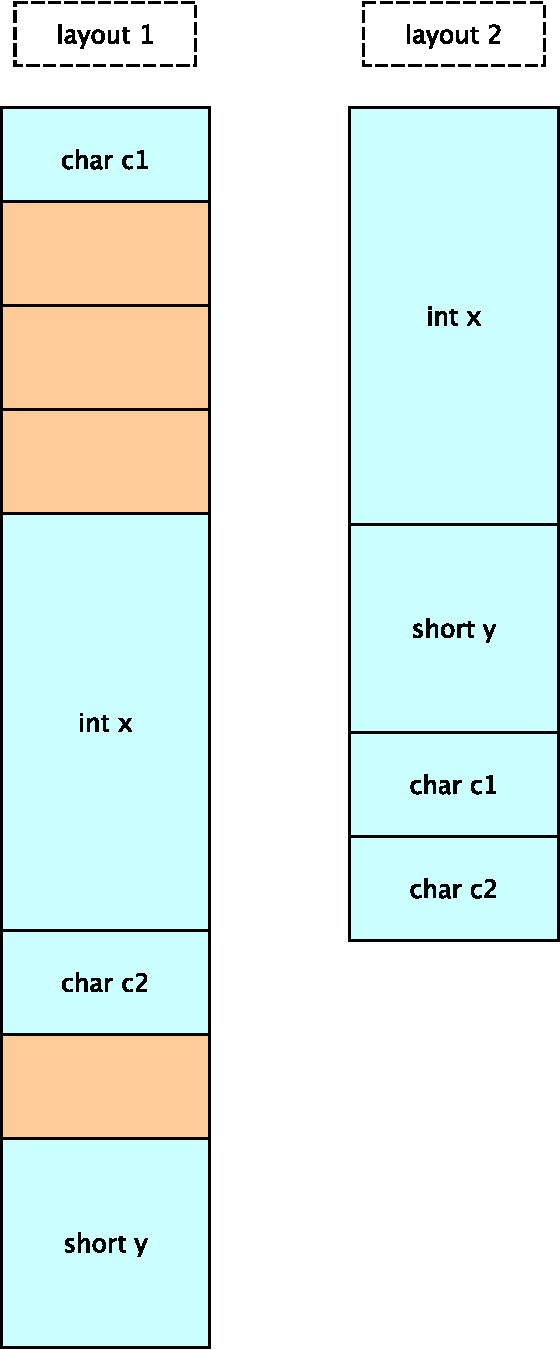
\includegraphics[width=0.4\textwidth]{illustrations/alignment-crop.pdf}
\caption{Два способа выравнивания}
\label{fig:alignment}
\end{figure}

На том же рисунке показано, что простое переупорядочение переменных с учетом выравнивания позволяет сэкономить довольно много места.

Всё то свободное место, которое компилятор оставляет пустым для выравнивания называется заполнителем (padding). В структуре padding обычно идёт между элементами или в самом конце структуры. Например на (рис. \ref{fig:alignment}) заполнители отмечены желтым.

\textbf{Вопрос к студентам:} сколько можно сэкономить на переупаковке вот такой структуры для 32-х битной машины?

\begin{lstlisting}
struct foo {
  char c;
  char *p;
  short x;
};
\end{lstlisting}

\ifanswers
Правильный ответ: переупаковка в нисходящем порядке

\begin{lstlisting}
struct foo {
  char *p;
  short x;
  char c;
};
\end{lstlisting}
\fi

Даст сокращение с 12 до 8 байт. Это уменьшение расхода памяти на 30\% (для массива в котором таких структур сто тысяч такое может быть заметно).

\textbf{Вопрос к студентам:} решите ту же задачу для 64-битной а не 32-битной архитектуры.

\ifanswers
Правильный ответ: теперь указатель будет 8 байт и скоращение с 24 до 16 -- те же 30\%
\fi

Структура как целое также имеет своё выравнивание (обычно оно соответствует наибольшему из требований членов структуры).

\textbf{Вопрос к студентам:} cтудент Шустрый предлагает такое переупорядочение структуры с использованием вложенной структуры

\begin{lstlisting}
struct foo {
  struct foo_inner {
    char *p;
    short x;
  } inner;
  char c;
};
\end{lstlisting}

Сколько займет такая структура в памяти 32-х битной машины?

\ifanswers
Ответ: выравнивание внутренней структуры получается 2, а выравнивание внешней структуры 7. Несложный подсчет показывает, что используется целых 16 байт. Немыслимо много. Поэтому с вложенными структурами надо быть осторожней.
\fi

Ещё одна сложность кроется в работе с битовыми полями:

\begin{lstlisting}
struct foo {
  int flip:1;
  int nybble:4;
  int septet:7;
  short s;
  char c;
};
\end{lstlisting}

С точки зрения компилятора здесь битовые поля образуют слово, в котором задействованы 12 бит из 16 возможных. В итоге в памяти 32-битной машины, эта структура займет 8 байт. Всё становится гораздо хуже если битовое поле пересекает границу слова.

\begin{lstlisting}
struct foo {
  int bigfield:30;
  int septet:7;
  short s;
  char c;
};
\end{lstlisting}

Такая раскладка заставляет компилятор разместить \lstinline!septet! в отдельное машинное слово и структура вырастает до 12 байт, из которых 32 бита уходят на семибитное поле.

\textbf{Вопрос к студентам:} Когда для какой-либо структуры вызывается \lstinline!sizeof!, как вы думаете, он возвращает размер с учётом выравнивания и заполнения или без учёта? И почему.

\ifanswers
Правильный ответ: с учётом. Потому что иначе например не работала бы идиома \lstinline!malloc(sizeof(widget))! -- здесь выделялось бы динамической памяти меньше, чем реально нужно.
\fi

\textbf{Вопрос к студентам:} более хитрый вопрос: а возможно ли вообще написать \lstinline!sizeof_unaligned! в сколь бы то ни было переносимом виде?

\ifanswers
Правильный ответ автору неизвестен. Скорее всего нет, но никто не исключает наличие какого-нибудь особо хитрого трюка.
\fi

Для C90, 6.2.6.1/6 явно гласит, что при записи любого значения в структуру, биты её паддинга принимают unspecified значение. Этот же пункт был унаследован всеми стандартами C и C++.

\textbf{Вопрос к студентам:} рассмотрим структуру

\begin{lstlisting}
struct Padded { int x; char y; };
\end{lstlisting}

В предположении, что \lstinline!sizeof(char) == 1! и архитектура выравнена на 4 байта, какой размер заполнителя она будет иметь?

\ifanswers
Правильный ответ: 3 байта.
\fi

\textbf{Вопрос к студентам:} допустим структура явно заполнена нулями

\begin{lstlisting}
struct Padded p;
memset (&p, 0xDA, sizeof(p));
\end{lstlisting}

Заполнится ли при этом значениями \lstinline!0xDA! её паддинг?

\ifanswers
Верный ответ: да, несомненно.
\fi

\textbf{Вопрос к студентам:} теперь допустим, что некое значение записывается в одно из полей структуры: \lstinline!p.x = 2!. Можно ли теперь полагаться, что в паддинге осталось значение \lstinline!0xDA!?

\ifanswers
Верный ответ: нет, потому что см. выше, при записи в поля, паддинг unspecified.
\fi

\subsection{Прокачка перечислений}\label{EnumClass}

Стандартные перечисления хороши, но не без проблем: во-первых они неявно конвертируются в \lstinline!int!, таким образом создавая возможность использовать их не по назначению. Во-вторых они экспортируют имена своих перечислителей в окружающую область видимости, создавая таким образом конфликты имен. В-третьих они не типизированы.

Последнее -- самая мрачная проблема:

\begin{lstlisting}
enum E_MY_FAVOURITE_FRUITS {
     E_APPLE      = 0x01,
     E_WATERMELON = 0x02,
     E_COCONUT    = 0x04,
     E_STRAWBERRY = 0x08,
     E_CHERRY     = 0x10,
     E_MY_FAVOURITE_FRUITS_FORCE8 = 0xFF
};
\end{lstlisting}

Намерение программиста здесь понятно: хочется, чтобы перечислимый тип был восьмибитным. Но каким он окажется в реальности? Это зависит от реализации и тут вполне можно ожидать 32 бит.

Все эти проблемы решает появившаяся в C++11 конструкция \lstinline!enum class!.

\begin{lstlisting}
enum class E_MY_FAVOURITE_FRUITS : 
  unsigned char {
    E_APPLE        = 0x01,
    E_WATERMELON   = 0x02,
    E_COCONUT      = 0x04,
    E_STRAWBERRY   = 0x08,
    E_CHERRY       = 0x10,
    E_DEVIL_FRUIT  = 0x100, // Warning!
};
\end{lstlisting}

Здесь двоеточие используется для указания нижележащего типа. Таким образом компилятор может выдать предупреждение о несоответствии типов, что может спасти много времени в отладке, а программист может сэкономить на размере. 

\pagebreak
\section{Автоматический вывод типов}\label{TypeInference}\index{Type inference}

\hfill\textit{Whatever we know without inference is mental}{\vspace{0.5em}}

\hfill\textit{-- Bertrand Russel}

Вывод типов (type inference) это базовое и очень впечатляющее усовершенствование в стандарте C++11, которое легко понять и легко использовать. Базовая идея просто как правда: вместо того, чтобы указывать компилятору тип, мы даём компилятору свободу вывести допустимый статический тип из контекста определения. С одной стороны это связывает руки: в таких контекстах объявление должно совпадать с определением всегда-всегда. Но с другой стороны, это даёт существенную свободу -- свободу не думать о том, какой в этом месте использован тип и почему он там использован. Для многих случаев это очень важно и почти все современные статически типизированные языки дают возможность такого полезного умолчания. Добавление таких возможностей в C++ было неизбежно, а их разумное использование будет для вашей программы благоприятно.

\subsection{Auto и Decltype}\label{DecltypeAuto}

Одной из главных сильных черт C++ является его сильная типизированность. Тем не менее часто она утомительна. 

\begin{lstlisting}
typedef uint_least8_t decl_handler_t;
decl_handler_t query_resource (int x);
\end{lstlisting}

Теперь каждый раз когда нужно вызвать \lstinline!query_resource!, нужно вспоминать и заводить в программе переменную правильного типа. Или рисковать проблемами, используя для результата \lstinline!int!.

Но казалось бы, компилятор же знает этот тип. Почему его нельзя просто вывести автоматически? В конце концов это работает для шаблонных функций.

\begin{lstlisting}
template <typename T> 
void bar (T x);

bar (query_resource(0));
\end{lstlisting}

Здесь будет сгенерирована по шаблону и вызвана функция \lstinline!bar!, параметризованная типом \lstinline!decl_handler_t!. Начиная с C++11 то же самое можно делать для переменных, заводя для них специальный (автоматический) тип.

\begin{lstlisting}
auto x = query_resource(0);
\end{lstlisting}

Теперь тип переменной \lstinline!x! правильно выводится из реального возвращаемого типа \lstinline!query_resource!, каким бы он ни был.

Если компилятор может взять тип выражения, логично, что это должен уметь и пользователь. Предыдущий кусок кода может быть переписан так:

\begin{lstlisting}
auto i = query_resource(0);
decltype(i) j = i++;
\end{lstlisting}

Здесь на второй строчке объявлено ``сделать j такого же типа, как i''. Это может быть полезно не только для уменьшения кода, но и для облегчения его поддержки:

\begin{lstlisting}
/* maybe in future type of a will change */
void foo (int a)
{
    /* type of b should be type of a */
    decltype(a) b;
    /* do something with b */
}
\end{lstlisting}

Без \lstinline!decltype! можно банально забыть консистентно исправить типы по всей функции и попасть на неприятные и плохо диагностируемые компилятором ошибки при смешивании знаковых и беззнаковых или типов разного размера.

Иногда \lstinline!decltype! может быть сопряжен с некоторыми концептуальными проблемами.

\begin{lstlisting}
struct Point { int x, y; };
Point porig {1, 2};
/* ... */
const Point &p = porig;
decltype(p.x) x; /* int or const int&? */
\end{lstlisting}

\textbf{Тема для обсуждения:} представьте, что вы в комитете по стандартизации. Предложите аргументы в пользу первого и в пользу второго понимания \lstinline!decltype!, проголосуйте.

Это действительно предмет для спора, так как опытный программист может аргументировать и ту и другую позицию. Автор проводил лекции на эту тему и мнения аудитории обычно разделялись в соотношении примерно 60/40 (причем человеческая интуиция работает \textbf{не} в пользу того варианта, который реально принят в стандарте).

Для разрешения этой неоднозначности, стандарт вводит (7.1.6.2) дополнительную форму \lstinline!decltype! с двумя круглыми скобками:

\begin{lstlisting}
decltype(p.x) x; /* int */
decltype((p.x)) x; /* const int& */
\end{lstlisting}

Следует обратить внимание, что, вторая строчка является ошибкой компиляции, так как объявляет неинициализированную ссылку.

На самом деле это различие более тонкое чем просто ещё одни скобки (это была бы слишком грешная магия даже для C++). Речь идёт о разнице между \lstinline!decltype(id-expr)! и \lstinline!decltype((expr))!. Первое возвращает тип, с которым было объявлено имя, второе -- тип, который могло бы приобрести выражение при его вычислении. Как сделать имя выражением? Обернуть его скобками, очевидно. Это кажется некоторым переусложнением, но это на самом деле единственный разумный выход из ситуации. Увы, \lstinline!decltype((expr))! имеет неприятную и с первого взгляда необоснованную особенность -- если тип под ним это lvalue, то он добавит ссылку (если её не было)

\begin{lstlisting}
int x;
typedef decltype(x) xval; /* int */
typedef decltype((x)) xref; /* int& */
typedef decltype((x+1)) xval_again; /* int */

xval r0;
xref r1 = x;
xval_again r2;
\end{lstlisting}

Мотивация для такого поведения станет ясна несколько позже (см. обсуждение в \ref{DeclFunctions}). Но интуитивно это уже ясно -- подчеркивается возможность присваивания. Между прочим выражение ``могло бы быть'' зафиксировано в стандарте и это даёт забавные возможности. Скажем \lstinline!decltype(10000000)! это ``целый тип в котором могло бы поместится 10000000''. Компилятор не обязан выводить наименьший целый тип, но обычно это происходит (в GCC это происходит всегда).

\textbf{Вопрос к студентам:} как насчет \lstinline!decltype((x+y))! если оба \lstinline!int!?

\ifanswers
Правильный ответ: конечно же сумма это не lvalue.
\fi

Вывод типов в C++ работает гораздо более приблизительно, чем их прямая аннотация, поэтому \lstinline!auto! часто выводит первый попавшийся (на самом деле -- наименее общий о чем см. далее) тип, а вот \lstinline!decltype! всегда старается сохранить даже cv-квалификацию

\begin{lstlisting}
  const int s = 5;
  auto s1 = s;
  decltype (s) s2 = 3;
  s1 += 1;
  /* s2 += 1; */
\end{lstlisting}

Строчка \lstinline!auto s1 = 3! ничего не изменит.

Разумное применение этих средств позволяет существенно улучшить читаемость вашего кода и сделать гораздо меньше тонких ошибок и опечаток в сложных именах типов. Но тут нужно учитывать, что всегда есть тонкости и волчьи ямы. Я рассказал как ведет себя \lstinline!auto!, но \lstinline!auto! ведет себя так не всегда. Если вы конкретизируете тип, то все квалификаторы сохранятся вместе с вашей конкретизацией:

\begin{lstlisting}
const int c = 0;
auto& rc = c;
rc = 44; // error: const qualifier was not removed
\end{lstlisting}

Также, и это бывает неприятно, \lstinline!auto! склонно пропускать модификаторы если на верхнем уровне оно встречает то, к чему они относятся:

\begin{lstlisting}
int x = 42;
const int* p1 = &x;
auto p2 = p1; /* p2 is const int* */
p2 = &y; /* ok */
/* *p2 = 3; */
\end{lstlisting}

Язык C++ справедливо считает, что константность данных под указателем это слишком важная характеристика типа. В отличии от этого, константность самого указателя может быть сброшена легко:

\begin{lstlisting}
const int* const p1 = &x;
auto p2 = p1; /* p2 is const int* */
p2 = &y; /* ok */
\end{lstlisting}

Разные правила для \lstinline!decltype! и \lstinline!auto! привели в стандарте C++14 к введению идиомы \lstinline!decltype(auto)! которая позволяет вывести тип из правой части автоматически, но именно так, как его вывел бы \lstinline!decltype!.

\begin{lstlisting}
const int i;
auto j = i; /* typeof(j) == int */
decltype (auto) k = i; /* typeof (k) == const int */
\end{lstlisting}

Очень интересный случай это выражение справа от \lstinline!decltype!, заключенное в круглые скобки.

\begin{lstlisting}
int i;
auto x4a = (i); /* decltype(x4a) is int */
decltype(auto) x4d = (i); /* decltype(x4d) is int& */
\end{lstlisting}

Таким образом моделируется поведение двух круглых скобок у выражения \lstinline!decltype! с конкретным \lstinline!t!.

В качестве вишенки на торте, \lstinline!auto! на самом деле достаточно мощно, чтобы замещать тип во всех контекстах (пример из стандарта C++14 раздел 5.3.4.2)

\begin{lstlisting}
auto x = new auto('a');
\end{lstlisting}

Здесь выведенным значение будет \lstinline!char!. Интересно дальше:

\begin{lstlisting}
auto x1 = { 'a', 'b' };
\end{lstlisting}

\textbf{Вопрос к студентам:} Что будет выведено здесь? 

\ifanswers
Это довольно хитрый вопрос. Ответ ``массив'' неверный. В реальности будет выведен \lstinline!std::initializer_list<char>! -- тот самый новый тип, который позволил так лихо инициализировать вектор в самом начале.
\fi

Интересно, что это -- единственное место, где отличается вывод типов шаблонами (см. \ref{TypeInference}) и \lstinline!auto!. Для шаблонного параметра здесь будет ошибка.

\textbf{Вопрос к студентам:} известно, что в случае обычных типов их можно перечислять через запятую в одном определении. Как вы думаете, какой тип будет выведен здесь?

\begin{lstlisting}
auto x = 5, *y = &x;
\end{lstlisting}

\ifanswers
Вопрос несколько более простодушен. Правильный ответ: увы, это ошибка. Это, правда, создает некоторые проблемы. Неясно почему вот так можно:

\begin{lstlisting}
auto x = 1; 
auto y = 1.0;
\end{lstlisting}

А вот так нельзя:

\begin{lstlisting}
auto x = 1, y = 1.0; /* ! */
\end{lstlisting}

Написано-то как бы одно и то же. Ждем исправления этого в C++17 или более поздних. С другой стороны, жить это не мешает.
\fi

\subsection{Расширенный синтаксис функций}\label{DeclFunctions}

Возможности автоматического вывода типов подразумевают построение абстракций с зависимыми типами. Пусть необходим статический шаблонный контракт на любой тип \lstinline!T!, поддерживающий функцию \lstinline!T::makeobject!, возвращающую некий свой тип. Нельзя (по крайней мере в стандарте C++11) просто взять и написать:

\begin{lstlisting}
template <typename T> auto /* Error! */
makeAndProcessObject (const T& builder)
{
    auto val = builder.makeObject();
    /* do stuff with val */
    return val;
}
\end{lstlisting}

Потому что компилятор в точке объявления функции не обладает информацией о типе, который вернет \lstinline!T::makeobject!. Забегая вперед -- иногда обладает, скажем в C++14 тут все хорошо. Точно так же не сработает вот такой выход:

\begin{lstlisting}
template <typename T> 
decltype(builder.makeObject()) /* Error again! */
makeAndProcessObject (const T& builder)
\end{lstlisting}

Потому что \lstinline!builder! не может быть использован до точки своего объявления (которой является список аргументов функции). Конечно правильного прошаренного пацана это не остановит. Он использует тот факт, что значение под \lstinline!decltype! не вычисляется, и сделает тонко:

\begin{lstlisting}
template <typename T> 
decltype (((T*)0)->makeObject()) /* painfull but works */
makeAndProcessObject (const T& builder)
\end{lstlisting}

Но нельзя требовать от программистов такое всерьез, всегда и везде. Комитет по стандартизации решил эту проблему изящно, предложив расширенный синтаксис для обобщённых функций, возвращающих зависимые типы:

\begin{lstlisting}
template <typename T> auto
makeAndProcessObject (const T& builder) -> decltype (builder.makeObject())
{
    auto val = builder.makeObject();
    /* do stuff with val */
    return val;
}
\end{lstlisting}

Внутри скобок \lstinline!decltype! в данном случае вычисление выражения (в том числе вызов функции) не происходит -- происходит только вывод типа.

Выбор правильного результата для гетерогенных функций это большое дело, например:

\begin{lstlisting}
template<typename A, typename B> 
auto add(A const& a, B const& b) -> decltype(a + b) 
{ 
  return a + b; 
}
\end{lstlisting}

Этот подход будет работать во всех случаях, когда входные типы допускают сложение.

Конечно, здесь есть возможные ошибки и засады:

\begin{lstlisting}
template <typename T, typename S>
auto min(T x, S y) -> decltype(x < y ? x : y) 
{
  return x < y ? x : y;
}
\end{lstlisting}

Казалось бы все при всем, но так писать нельзя, поскольку \lstinline!decltype! вокруг выражения работает как \lstinline!decltype(expr)!, а значит результат может быть выведен как ссылка, что чревато. Так как же все таки правильно написать type-generic minimum? Эта проблема найдет свое решение позже (см. \ref{ReferenceConvolution}).

\textbf{Вопрос к студентам:} Представим, что \lstinline!T! и \lstinline!S! это простые типы без квалификаций, указателей ссылок и прочего добра. Просто  \lstinline!int!, \lstinline!double! и всё такое. В каких случаях  \lstinline!decltype! здесь выведет ссылку, а в каких нет? 

\ifanswers
Правильный ответ: ссылка будет если типы одинаковые. Если они разные, все будет хорошо.
\fi

Зато теперь можно понять почему же такое поведение \lstinline!decltype(expr)! было выбрано комитетом по стандартизации. Рассмотрим упрощенную задачу -- допустим речь идет о выводе типа для доступа к элементу массива:

\begin{lstlisting}
template <typename T>
auto array_access(T& array, size_t pos) -> decltype(array[pos]) 
{
  return array[pos];
}
\end{lstlisting}

С текущим подходом можно использовать такую обертку прозрачно как если бы это действительно был доступ к элементу массива:

\begin{lstlisting}
std::vector<int> vect = {42, 43, 44};
int* p = &vect[0];

array_access(vect, 2) = 45;
array_access(p, 2) = 46;
\end{lstlisting}

В противном случае пришлось бы идти на разнообразные хаки.

Позвольте еще маленькую вишенку на этот тортик:

\begin{lstlisting}
auto main() -> int
\end{lstlisting}

Теперь является легитимной формой функции \lstinline!main! и если вы хотите показать насколько вы круче остальных людей в этом мире, то вы теперь знаете, что делать.

Впрочем, это так, отвлечение. Последний стандарт привнес ещё больше радости.

\subsection{Обобщения вывода типов функциями}\label{Auto14}

В некоторых простых случаях компилятору действительно не составляет проблем вывести тип функции: 

\begin{lstlisting}
auto isquare (int x) -> decltype (x) { 
  return x*x;
}
\end{lstlisting}

Здесь указание \lstinline!decltype! выглядит просто излишним и C++14 разрешает его убрать:

\begin{lstlisting}
auto isquare (int x) { return x*x; }
\end{lstlisting}

Для таких простых вариантов все хорошо, но как быть с рекурсией? Здесь возникает проблема: тип должен быть выведен до того, как рекурсивный вызов произошел:

\begin{lstlisting}
auto sum_to (int i) {
  if (i < 2)
    return i; // return type deduced as int
  else
    return sum_to (i-1) + i;  // ok to call it now
}

cout << sum_to (10) << endl;
\end{lstlisting}

Но если переставить возвраты в вышеприведенном коде, он не будет скомпилирован.

\begin{lstlisting}
auto bad_sum_to (int i) {
  if (i > 2)
    return bad_sum_to (i-1) + i;
  else
    return i;
}
\end{lstlisting}

Впрочем, GCC возвращает вполне человечное описание ошибки

\begin{verbatim}
error: use of ‘auto bad_sum_to(int)’ before deduction of ‘auto’
     return bad_sum_to (i-1) + i;
\end{verbatim}

С 2014 года также нет проблем с тем, чтобы шаблонные методы выводили свой тип непосредственно из других методов того же класса без явного \lstinline!this! (пример взят из стандарта C++14, 5.1.1.3)

\begin{lstlisting}
struct A {
  char g();
  template <typename T> auto f(T t) { 
    return t + /* this-> */ g();
  }
};
\end{lstlisting}

Одно опасное заблуждение связано с идеей использовать \lstinline!auto! в списке параметров функции (не лямбды, для лямбд всё хорошо, см. \ref{GenericLambdas})

Люди пишут нечто вроде следующего кода (обратите внимание на auto в списке параметров), предполагая, что компилятор выведет нечто из аргумента по умолчанию.

\begin{lstlisting}
auto foo (auto x = 1) { return x; }
\end{lstlisting}

Во-первых это вообще не C++. Во-вторых, это скомпилируется только благодаря популярному расширению в GCC которое ввели, когда казалось, что в 2017 году такой синтаксис примут в стандарт (нет, не приняли). В третьих, даже как расширение это будет работать вот так

\begin{lstlisting}
template <typename T> auto foo (T x = 1) { return x; }
\end{lstlisting}

То есть никакого вывода до точк вызова. Здесь \lstinline!auto! в списке типов просто заменяет явный шаблонный аргумент.

Это крайне неочевидный синтаксис, он был плох для включения в стандарт, он плох как расширение, не надо так делать.

\subsection{Точный вывод и прозрачная оболочка}\label{DecltypeAuto14}

Увы, как уже было сказано \lstinline!auto! режет типы

\begin{lstlisting}
auto Example(int const& i) { return i; }
\end{lstlisting}

Здесь возвращаемый тип \lstinline!int!. Конечно, в конкретном коде несложно вернуть квалификацию типа:

\begin{lstlisting}
auto const& Example(int const& i) { return i; }
\end{lstlisting}

Но что делать в обобщенном коде?

В обобщенном коде для точного вывода возвращаемого типа может быть использован \lstinline!decltype (auto)! например так:

\begin{lstlisting}
template <typename Fun, typename Arg>
decltype(auto) transparent(Fun fun, Arg arg) { 
  return fun(arg); 
}
\end{lstlisting}

Теперь тип возвращаемого значения будет проброшен точно. Ниже будет показано как написать совершенно прозрачную обертку: пробросив не только возвращаемое значение но и произвольные аргументы (см. \ref{PerfectForw}).

\subsection{Decaying и минимальные общие типы}\label{Decaying}\index{Decay function}

Decaying уже был рассмотрен, при рассмотрении деградации массивов в указатели (\ref{ArrDecaying}), но если в старом стандарте это была built-in особенность для одной конкретной пары типов, то новый стандарт предлагает интересные варианты обобщения этого понятия на любые типы. Простой случай:

\begin{lstlisting}
int foo (const int &s) { return s + 2; }
\end{lstlisting}

Здесь в выражении \lstinline!s + 2!, \lstinline!s! ведёт себя так, как будто его тип \lstinline!int!. Тогда можно сказать, что \lstinline!const int &! деградирует к \lstinline!int! в том же смысле, в каком массив деградирует к указателю, etc. Новый стандарт позволяет вручную ``деградировать'' тип:

\begin{lstlisting}
const int &i;
std::decay<decltype(i)>::type j; // int j 
auto k = i;                      // int k = i;
\end{lstlisting}

Автоматический вывод также осуществляет деградацию типов. Поэтому можно считать \lstinline!decay! + \lstinline!decltype! способом вывести тот тип, который вывело бы \lstinline!auto!.

На механизме \lstinline!decay! неявно построен механизм \lstinline!common_type!, позволяющий вывести минимальный общий тип:

\begin{lstlisting}
template <typename T, typename S> void foo(T lhs, S rhs) {
  std::common_type<decltype(lhs), decltype(rhs)>::type k;
  // .... etc ....
}
\end{lstlisting}

В принципе минимальные общие типы не так уже и нужны

\begin{lstlisting}
template <typename T, typename S>
void foo(T lhs, S rhs) {
  auto prod = lhs * rhs;
  //...
}
\end{lstlisting}

Устроит не менее качественную деградацию. Мало того, такое расширение GCC давно известное и во многих других компиляторах как \lstinline!typeof!, позволяло делать это и в старом стандарте. В новом же можно использовать \lstinline!decltype!.

\begin{lstlisting}
typedef typeof(lhs * rhs) product_type;
typedef decltype(lhs * rhs) product_type;
\end{lstlisting}

В качестве полезного примера, можно привести смешанную арифметику для числового класса:

\begin{lstlisting}
template <typename T> struct Number { T n; };
 
template <typename T, class U>
Number<typename std::common_type<T, U>::type> 
operator+(const Number<T>& lhs,
          const Number<U>& rhs) {
  return {lhs.n + rhs.n};
}
 
int main() {
  Number<int> i1 = {1}, i2 = {2};
  Number<double> d1 = {2.3}, d2 = {3.5};
  std::cout << "i1i2: " << (i1 + i2).n 
            << "\ni1d2: " << (i1 + d2).n 
            << "\nd1i2: " << (d1 + i2).n 
            << "\nd1d2: " << (d1 + d2).n 
            << '\n';
}
\end{lstlisting}

\textbf{Домашняя наработка:} проанализировать вывод этой программы и то, почему он ведет себя именно так.

\ifoutreach
\section{За пределами ISO C++}\label{subsec:outborders}

TODO: gnu extensions, boost
\fi

\pagebreak
\section{Домашняя наработка по базовому C++}

\textbf{Контрольные вопросы} 

\begin{enumerate}
\item Запишите волатильный указатель на массив целых чисел
\item Приведите пример когда использование typedef серьёзно улучшает читаемость кода
\item В каких случаях программист на C++ вынужден пользоваться макросами?
\item В чем преимущество констант над перечислениями?
\item Возможна ли инлайн-подстановка нестатической функции, определенной в другой единице трансляции?
\item В каких случаях вызов функции вместо подстановки идентичного макроса ускоряет работу кода?
\item Может ли объявление структуры располагаться внутри определения функции?
\item Может ли время жизни объекта заканчиваться раньше достижения границ его области видимости?
\item Можно ли использовать ссылку на неполный тип в определении функции?
\item Может ли вызов функции быть lvalue?
\item Можно ли вычислить побитовое или двух указателей?
\item Возможно ли иметь в программе массив из ссылок?
\item Возможна ли ссылка на массив?
\item Всегда ли можно получить указатель на нечто, на что существует ссылка?
\item В каких случаях нельзя заменить static cast на const cast?
\item Может ли функция быть перегружена по cv-квалификатору аргумента?
\item Можно ли расширить пространство имен, определяемое структурой?
\item Есть ли разница в выводе типа auto из правой части или правой части в дополнительных скобках?
\item Можно ли использовать auto в полях структур?
\item Какой тип будет выведен для пустой строки?
\item Какие преимущества имеет новый синтаксис объявления функций?
\item Какой тип является минимально общим между ссылкой на int и ссылкой на float?
\end{enumerate}

\textbf{Задания} 

\begin{enumerate}
\item
Дана структура данных, воплощающая простой односвязный список

\begin{lstlisting}
typedef struct list_tag
{
  void *data;
  struct list_tag *next;
} list_t, *list_p;
\end{lstlisting}

У последнего элемента \lstinline!next = 0!

Необходимо написать на языке C++ функцию, берущую на вход указатель на голову списка и переворачивающую список в памяти, так, что первый элемент становится последним, второй предпоследним и так далее.

\item
Дана программа на языке C с комментариями вида \lstinline!/* comment */!

Необходимо написать на языке C++ программу, выкидывающую все комментарии из текста данной.

\item
Дана структура данных, соответствующая n-арному дереву

\begin{lstlisting}
typedef struct tree_tag
{
  void *data;
  struct tree_tag *top;
  struct tree_tag **childs;
} tree_t, *tree_p;
\end{lstlisting}

Реализуйте на языке C++ функцию, берущую на вход пару указателей на произвольные элементы дерева, и подсчитывающую расстояние между ними (минимальный путь в дереве). Как вы будете тестировать эту функцию?

\item
Реализуйте на языке C++ алгоритм из (\ref{AlgDecl}) и протестируйте на нескольких сотнях сгенерированных определений

\item
Реализуйте на языке C++ транспонирование двумерной матрицы

\item
Реализуйте на языке C++ операцию получения двумерной матрицы обратной данной

\item
Реализуйте на языке C++ операцию умножения вектора на матрицу

\item
Реализуйте на языке C++ калькулятор, делающий вычисления в обратной польской нотации. Например \lstinline!1 2 3 4 + * + =! должно выдавать 25 в качестве результата.

\item
Известны год, месяц и день рождения человека. Реализуйте на языке C++ программу, определяющую его возраст в днях на текущую дату.

\item
Реализуйте на языке C++ программу, подсчитывающую количество лет в 20-м веке у которых первым днём было воскресенье

\item
На вход дана строка из \lstinline!N*N! символов. Реализуйте на языке C++ функцию, выделяющую в памяти двумерную матрицу \lstinline!N*N! и заполняющую её последовательными данными из входной строки.

\item
На вход даны завершающаяся нулём строка \lstinline!haystack! и завершающаяся нулём строка \lstinline!needle!. Реализуйте на языке C++ функцию, определяющую, является ли \lstinline!needle! подстрокой \lstinline!haystack!

\item
В условиях предыдущей задачи необходимо доработать функцию, чтобы она выкидывала из \lstinline!haystack! все вхождения \lstinline!needle! и возвращала измененную строку.

\item
Напишите на C++ программу, которая будет возвращать номер в последовательности Фибоначчи первого числа имеющего 1000 разрядов в десятичном представлении.

\end{enumerate}

\pagebreak
\chapter{Объектно-ориентированное счастье}\label{chap:OOP}

\hfill\textit{I made up the term 'object-oriented',}

\hfill\textit{and I can tell you I didn't have C++ in mind} {\vspace{0.5em}}

\hfill\textit{-- Alan Kay, OOPSLA '97}

Как известно, самой целью создания C++ Бьёрном Строструпом было добавление объектно ориентированных возможностей к C, поэтому изначально язык назывался ``C с классами''. Известно также, что Строструп вдохновлялся языком Simula, но сейчас уже нельзя оценить насколько это была удачная идея, поскольку этот язык канул в лету (зато известна вынесенная в эпиграф цитата одного из гуру ООП). Так или иначе, но C++ действительно обладает уникальной среди современных объектно ориентированных языков моделью объявления и инстанциирования классов. Многим нравится богатство и гибкость её возможностей, многие в ужасе отползают. Эта глава посвящена особенностям ООП в C++ и является центральной темой первого семестра обучения.

\pagebreak
\section{Инкапсуляция и игра в мячик}\label{Encapsulation}

\hfill\textit{I find OOP philosophically unsound.}

\hfill\textit{It claims that everything is an object.}

\hfill\textit{Even if it is true it is not very interesting.} {\vspace{0.5em}}

\hfill\textit{-- Alex Stepanov}

Пусть стоит задача разработать тип данных, который будет использован для моделирования полёта материальной точки в двумерном мире (высота, длина). Мяч может лететь свободно, для чего у него вызывается метод \lstinline!fly(double t)! или его можно толкнуть, придав ему определённую скорость под определённым углом (после чего например опять отправить в полёт и так далее). Можно написать определение структуры, вроде приведенного ниже.

\begin{lstlisting}
struct ball {
  double t;
  double vx;
  double vy;
  double x;
  double y;
  void push(double v, double alpha);
  void fly(double time);
};
\end{lstlisting}

Представляет ли эта структура данных хорошую абстракцию мяча? Нет, не представляет. Каждый пользователь вашего ``мяча'' может произвольно менять его координаты. Это означает, что в плохо отлаженной программе симуляции, этот мяч сможет свободно ``телепортироваться'', а это явно не то, чего ждут от законченной модели. 

\begin{lstlisting}
ball foo() {
  ball a_ball;
  a_ball.vx = 5.0; /* sad, but ok */
  a_ball.push(5.0, 0.75); /* ok */
  a_ball.x = -1.0; /* hmm... still ok */  
  return a_ball;
}
\end{lstlisting}

Хуже того, время может быть свободно переставлено вперёд или назад. Но пусть даже никто не ошибся и всё написано правильно. А потом... возникла необходимость ``запустить'' этот мяч в многопользовательской среде. Всё пропало – для того, чтобы вставить синхронизацию, переписывать придётся каждый участок кода где ссылались на эти поля.

\subsection{Конкретные классы}\label{ConcreteClasses}

Для разграничения состояния модели от её поведения и более гибкого управления поведением, в C++ были введены классы. Простые классы, без использования полиморфизма и без иерархий наследования, называются ``конкретными классами''. Конкретные классы -- мощный и полезный инструмент для поддержания консистентности абстракции. Можно переписать модель мяча, создав его класс

\begin{lstlisting}
struct ball_t {
private:
  double m_x;
  double m_y;
  double m_vx;
  double m_vy;
  double m_t;
public:
  void push(double a_v, double a_alpha);
  void fly(double a_time);
};
\end{lstlisting}

Модификатор \lstinline!public! означает, что любой пользователь типа \lstinline!ball_t! имеет доступ к этим методам или данным. 

Модификатор \lstinline!private! означает, что доступ к соответствующим методам и данным имеют только методы этого класса.

\begin{lstlisting}
void ball_t::push(double a_v, double a_alpha) {
  assert(a_v > 0);
  m_vx += a_v * cosf(a_alpha); /* ok */
  m_vy += a_v * sinf(a_alpha);
}

ball_t bar() {
  ball_t ball;
  ball.m_vx = 5.0; // FAIL
  ball.push(5.0, 0.75); // OK
  return ball;
}
\end{lstlisting}

Хорошим тоном считается закрывать данные, составляющие состояние объекта и открывать функции, составляющие его поведение.

\textbf{Вопрос к студентам:} вам приносят код, в котором автор написал класс, открывающий к полю как чтение так и запись:

\begin{lstlisting}
struct colored_ball_t {
private:
  int color_;
  // all other fileds ....
public:
  int get_color() { return color_; }
  void set_color(int color) { color_ = color; }
  // all other methods ....
};
\end{lstlisting}

Его коллега предлагает убрать обе функции и вынести поле \lstinline!color_! в открытую часть, так как оно всё равно не инкапсулировано. Что вы на это скажете?

\ifanswers
Правильный ответ: поле всё-таки инкапсулировано лучше, чем если просто торчит наружу. Например у него не может утечь адрес. Метод, который полностью вскрывает инкапсуляцию будет выглядеть так:

\begin{lstlisting}
public:
  int& color() { return color_; } // bad idea
\end{lstlisting}

и даже такой метод иногда имеет смысл оставить в классе (контроль доступа, логгирование, удобство отладки, вот это всё).
\fi

\textbf{Вопрос к студентам:} вы сидите в комитете и вам приносят пример:

\begin{lstlisting}
struct Bar {
private:
  int foo (int);
public:
  int foo (char);
};

Bar b;
b.foo(1);
\end{lstlisting}

Как по вашему: должна быть ошибка или вызов public функции?

\ifanswers
Правильный ответ: де-факто здесь будет ошибка. И это можно обосновать: представьте, вы решили закрыть доступ для некоего метода. Вы конечно хотели бы, чтобы во всех местах, где вы его использовали, была ошибка, но если по месту использования он может просто связаться с другой перегрузкой, её не будет.
\fi

\subsection{POD и NPOD типы}\index{POD}\index{NPOD}\label{PodNpod}

В языке C со структурами всё было довольно просто.

Из-за скрытия состояния и наличия нетривиального поведения, в языке C++ существует ряд категорий типов: типы со специальным созданием, со специальным поведением при копировании, с неизвестным или зависящим от реализации размером и так далее.

Стандарт определяет следующие термины (C++14, 9 раздел) для обозначения категорий типов, объекты которых могут быть созданы.

\begin{itemize}
\item \textbf{Тривиально копируемый} -- тип, непрерывный в памяти и не обладающий специальным поведением при копировании. Для таких типов работает \lstinline!memcpy! и \lstinline!memmove! 
\item \textbf{Тривиальный} -- тривиально копируемый тип без специального поведения при создании.
\item \textbf{Со стандартным расположением полей} -- тип, без зависящих от реализации полей (например без членов-ссылок, без таблиц виртуальных методов и так далее). Такие типы удобны для передачи в модули, написанные на других яызках программирования, например на C или Java -- их всегда можно десериализовать независимым от языка и компилятора образом.
\item \textbf{POD} -- от plain old data -- тривиально копируемый тип со стандартным расположением полей.
\end{itemize}

Все типы, не являющиеся POD называются NPOD (от not plain old data).

По мере введениях новых техник ООП, будет рассмотрено каким становится тип в зависимости от объявления.

Типы с закрытой частью остаются тривиально копируемыми.

\subsection{Инициализация и уничтожение\index{constructor}\index{destructor}}\label{subsub:constrdestr}

Отсутствие доступа к состоянию означает, что при создании объекта он должен уметь сам установить своё состояние, а при уничтожении – освободить свои ресурсы. Для этого в класс вводятся конструктор и деструктор – специальные функции, вызывающиеся при создании и уничтожении объекта. Например у класса мяча, конструктор может устанавливать начальное положение, деструктор же может быть тривиальным.

\begin{lstlisting}
ball_t(double a_x = 0.0, double a_y = 0.0):
  m_x(a_x), m_y(a_y), m_vx(0.0), m_vy(0.0), m_t(0.0) {}

~ball_t() {}
\end{lstlisting}

Обратите внимание на список инициализации у конструктора в этом примере кода. Можно, конечно, написать инициализацию в теле конструктора, но использование списков инициализации является лучшей идеей. По умолчанию, удовлетворяющий стандарту языка C++ компилятор сгенерирует конструктор (на самом деле несколько конструкторов) и деструктор по умолчанию. Это кажется удобным, но в \ref{RAII} последует обсуждение того, чем это может быть чревато. Конструктор по умолчанию вызывает конструкторы всех членов класса, у которых они есть, деструктор -- их деструкторы.

Здесь становится ясна упомянутая ранее (см. \ref{subsub:newdelete}) сила новых ключевых слов \lstinline!new! и \lstinline!delete!. При необходимости создать мячик на куче, обычный \lstinline!malloc! выделит память, но не вызовет конструктор. Единственный способ вызвать конструктор это использовать \lstinline!new!. Простейший способ получить мячик на куче:

\begin{lstlisting}
ball_t *pball = new ball_t(1.0, 2.0);
// use it here
delete pball;
\end{lstlisting}

Соответственно двадцать мячиков инициализированных по умолчанию получаются через вызов специального \lstinline!new! с квадратными скобками. Он не только вызывает конструкторы всех этих объектов, но ещё и записывает специальные структуры в памяти, чтобы сообщить следующему вызову \lstinline!delete[]! сколько деструкторов вызывать.

\begin{lstlisting}
ball_t *pballs = new ball_t[20];
// use it here
delete [] pballs;
\end{lstlisting}

В базовом ООП, выделение памяти и вызов конструктора неразрывны. Когда речь пойдёт о переопределении операторов, будет рассмотрена возможность тонкого управления выделением и освобождением памяти (см. \ref{subsec:newdeleteredef}) в том числе так называемые ``размещающие'' формы \lstinline!new!. Тогда окажется, что это не всегда так. Но пока что можно считать, что это так.

Очень часто масса конструкторов в классе делает одно и то же или почти одно и то же. В этих случаях, начиная с C++11, конструкторы можно \textbf{делегировать} -- то есть вызвать конструктор того же класса из списка инициализации.

\begin{lstlisting}
class X {
  int a;
public:
  X(int x) : a(x) { /* ... some logic ... */ }
  X(double x) : X(static_cast<int>(x)) { }
};
\end{lstlisting}

Во многих случаях, инициализация списком утомительна. Для того, чтобы сократить записи списков инициализации, была придумана инициализация в теле класса.

\begin{lstlisting}
class A {
  int a = 7;
  int b = 5;  
public:
   A() {} // sets a = 7, b = 5
   A(int a_val) : a(a_val) {} // sets b = 5
};
\end{lstlisting}

Она так же доступна начиная с C++11 и её очень хорошо использовать чтобы точно не оставить ни одного поля в неинициализированном состоянии.

Неожиданно сложным вопросом является вопрос о том, что делать если в конструкторе произошла ошибка. Короткий ответ: использовать исключения. Подробный ответ будет рассмотрен далее (см. \ref{subsub:ctorerrs}). Пока что предполагается, что все конструкторы в этом разделе очень просты и ошибок, требующих нелокальной обработки, в них просто не будет.

\subsection{Неявное преобразование типов и explicit}\label{Explicit}

Конструкторы также используются для задания неявного преобразования типа\index{implicit type cast}. Неявные преобразования есть и в C, там они называются type promotions, некоторые из них (действуют и в C++) сведены в таблицу ниже (здесь anytype это любой встроенный тип, совместимый по операции но не перечисленный выше):

\begin{lstlisting}
anytype `op` long double => long double `op` long double
anytype `op` double => double `op` double
anytype `op` float => float `op` float
anytype `op` unsigned long long => unsigned long long `op` unsigned long long
anytype `op` long long => long long `op` long long
anytype `op` unsigned long => unsigned long `op` unsigned long
anytype `op` long => long `op` long
anytype `op` unsigned int => unsigned int `op` unsigned int
anytype `op` int => int `op` int
\end{lstlisting}

Но в C++ неявные преобразования также пробуются компилятором для пользовательских типов. Определение в пользовательском типе конструктора, который может быть истрактован как конструктор с одним аргументом (считая аргументы по умолчанию частично подставленными всюду кроме первого аргумента), считается определением неявного преобразование из аргумента конструктора к этому типу. Это может иметь неприятные последствия:

\begin{lstlisting}
int emulateBall(ball_t b);

int foo() {
  emulateBall(1.0); // ??? but legal
}
\end{lstlisting}

Верный способ определить конструктор, чтобы явно заявить компилятору, что он не поддерживает неявного преобразования это определить его с ключевым словом \lstinline!explicit!

\begin{lstlisting}
explicit ball_t(double a_x = 0.0, double a_y = 0.0):
  m_x(a_x), m_y(a_y), m_vx(0.0), m_vy(0.0), m_t(0.0) {}
\end{lstlisting}

Это важное решение при проектировании и его надо принимать осознанно. Лепить \lstinline!explicit! куда ни попадя -- дурной тон (скажем это ключевое слово возможно но совершенно не нужно на конструкторе более чем с одним аргументом и без аргументов по умолчанию). Но иногда он очень нужен.

\subsection{Value-инициализация и Default-инициализация}\label{ValDefInit}

Тривиальные и нетривиальные типы требуют разной обработки во время выделения памяти. Когда пользователь пишет

\begin{lstlisting}
int *t = new int; /* t uninitialized */
int *pt = new int [10]; /* pt[.] uninitialized */
\end{lstlisting}

Он не ожидает, что будет вызвано десять конструкторов для целых чисел. Вместо этого ожидаемое поведение это десять неинициализированных объектов.

\begin{lstlisting}
struct SomeTriv
{
  int x;
};

SomeTriv *px = new SomeTriv; /* x uninitialized */
\end{lstlisting}

Аналогично никакого конструктора не будет вызвано и в этом случае. Но немного изменим структуру:

\begin{lstlisting}
struct SomeNTriv
{
  int x;
  ~SomeNTriv() {;}
};

SomeNTriv *px = new SomeNTriv; /* x initialized with 0 */
\end{lstlisting}

Поскольку в этой структуре есть деструктор, она теперь не тривиальна и для неё будет сгенерирован конструктор по умолчанию. Для того, чтобы сделать у тривиальных типов такое же поведение, разработчики языка предусмотрели указание пустых скобок для value-initialization:

\begin{lstlisting}
struct SomeTriv
{
  int x;
};

SomeTriv *px = new SomeTriv (); /* x initialized with 0 */
int *t = new int (); /* t initialized with 0 */
int *pt = new int [10](); /* 10 ints are initialized with 0 */
\end{lstlisting}

Это создаёт некоторую запутанность, зато даёт некий аналог \lstinline!calloc! для всех тривиальных типов. 

\subsection{Селекторы}\label{Selectors}

Отражает ли созданная до сих пор абстракция физический мяч? Всё ещё нет. Мяч в физическом мире обычно виден пользователю, у которого есть возможность считать его координаты. То есть нужны некоторые методы, которые будут, сохраняя состояние мяча, давать возможность прочитать его. Такие методы традиционно называются селекторами.

\begin{lstlisting}
double get_x() const { return m_x; }
double get_y() const { return m_y; }
\end{lstlisting}

Обратите внимание на const в их объявлении. Внутри объявленного таким образом метода изменить любое поле класса это ошибка компиляции. Исключение составляют поля, объявленные с ключевым словом \lstinline!mutable!, но им не стоит злоупотреблять при проектировании.

\textbf{Домашняя наработка:} найти нетривиальный случай, когда ключевое слово \lstinline!mutable! полезно и оправдано

Хорошей считается привычка делать селектором любой метод, который теоретически может быть селектором и по логике не должен менять внутреннего состояния объекта. Это позволяет дополнительные оптимизации в компиляторе и аннотирует  метод важной информацией для дальнейшего переиспользования.

\subsection{Статические члены в классе\index{static members}}\label{StaticMembers}

Данные в классе, образующие его состояние, называются атрибутами объектов класса, потому что каждый объект имеет свою копию такого поля (такое поле \lstinline!x! является только на самом деле \lstinline!this->x!). Именно поэтому методы в структуре или классе берут первым аргументом неявный указатель на тот объект, для которого они вызваны (см. \ref{CCppStructs}).

Но иногда необходимо иметь общий атрибут для всех объектов класса. В этом случае используется ключевое слово \lstinline!static!, которое в контексте класса означает, что методы и данные не зависят от \lstinline!this! и являются общими для всех объектов класса.

\begin{lstlisting}
class ball {
  // attributes
  int x, y;
  // static field
  static int ball_count;
public: 
  ball() : x(0), y(0) { ball_count += 1; }

  // static method
  static int get_count () { 
    return ball_count; 
  }
}

int ball::ball_count = 0;
\end{lstlisting}

Здесь каждый конструктор при создании очередного мяча увеличивает счетчик мячей и статический метод отдаёт этот счетчик. Можно обратить внимание, что он не \lstinline!const!. Это не опечатка, более того, он и не может быть константным: поскольку у такого метода нет объекта класса, он не может изменять состояние ни одного объекта.

\begin{lstlisting}
  static int get_count () { 
    x += 1; // oops? We have no this.
  }
\end{lstlisting}

Таким образом это отношение работает в одну сторону: все объекты класса имеют доступ к его статическим методам и данным но не наоборот (без специальных ухищрений).

По сути статические методы не сильно отличаются от глобальных функций. Единственное отличие -- у статических методов класса есть доступ к закрытому статическому состоянию класса. Точно так же и статические члены не сильно отличаются от глобальных переменных. Нужно обратить особое внимание на инициализацию статического члена вне класса. Это вполне естественно: такие вещи нельзя делать в  конструкторе, потому что статический член должен быть доступен даже если ни одного объекта ещё не создано.

Дополнительное определение где-то вне класса требуется даже если инициализации не нужно.

\begin{lstlisting}
struct S {
  static int x;
};

int S::x;
\end{lstlisting}

Это связано с тем, что выделение памяти в конструкторе (как для объектов классов и их полей) не происходит, но память должна быть где-то физически выделена. Надо быть осторожнее с ODR -- плохая идея делать это в заголовочнике.

Исключение оставлено для статических констант, объявляемых внутри классов. Они допускают инициализацию по месту объявления.

\subsection{Указатели на методы класса}

\hfill\textit{If you can’t program in a language with ugly warts,}

\hfill\textit{maybe C++ isn’t the language you should be programming in} {\vspace{0.5em}}

\hfill\textit{-- John Calb}

Указатели на статические методы класса по сути не отличаются от указателей на функции. Указатели на нестатические члены класса сложнее, потому что вызов по такому указателю должен содержать объект класса для которого производится вызов. Можно рассмотреть простой класс (даже без закрытой части) о котором известен один его метод.

\begin{lstlisting}
struct MyClass {
   int DoIt(float a, int b) const;
   // ....
};
\end{lstlisting}

Тип ``указатель на константный метод'' тогда может быть легко записан (звёздочка после двойного двоеточия может смутить, но это часть синтаксиса).

\begin{lstlisting}
typedef int (MyClass::*constif_t)(float, int) const;
using constif_t = int (MyClass::*)(float, int) const;
\end{lstlisting}

Теперь вызов состоит в получении указателя на метод и связывании его с объектом.

\begin{lstlisting}
constif_t ptr = &MyClass::DoIt;
MyClass c;
(c.*ptr)(1.0, 1);
\end{lstlisting}

Интересный синтаксис возможен если есть указатель на такой класс и указатель на его метод

\begin{lstlisting}
MyClass *d = &c;
(d->*ptr)(2.0, 2);
\end{lstlisting}

Это печально знаменитый оператор \lstinline!->*!, который осваивают немногие, но который получает вторую жизнь в контексте умных указателей.

\subsection{Объявления и определения классов}\label{DeclDefs}

Это важный момент, перекликающийся с затронутой в (\ref{DeclVsDef}) темой объявлений и определений. Объявление класса как неполного типа выглядит так:

\begin{lstlisting}
class ball_t;
\end{lstlisting}

С этого момента тип \lstinline!ball_t! можно использовать по правилам, прописанным в стандарте для неполных типов. Определение класса это объявление всех его методов и полей.

Но внутри определения класса, каждое объявление поля, статического поля или метода это его объявление. Определением нестатического члена считается конструктор класса (поэтому если членом класса является ссылка она должна быть инициализирована в списке инициализации конструктора). Определение метода может как встречаться внутри класса, так и быть вынесено вне его. Определение статического объекта всегда должно быть вне класса.

\textbf{Домашняя наработка:} свести весь код игры в мячик воедино, добиться работоспособности кода

\pagebreak
\section{Классы для управления ресурсами}\label{WrapClasses}

\hfill\textit{C++ is my favorite garbage collected language}

\hfill\textit{because it generates so little garbage}{\vspace{0.5em}}

\hfill\textit{-- Bjarne Stroustrup}

В идеальном мире, программа производит чистые вычисления над неограниченным входным потоком и записывает результаты в неограниченный выходной поток. Реальный мир вносит коррективы: хорошо написанная программа всегда работает в условиях недостаточности машинных ресурсов и должна сама заботиться о том, чтобы рационально управлять запросами и освобождением ресурсов. До сих пор основным видом ресурсов с которыми вы сталкивались была динамическая память. Хорошо написанная программа рационально выделяет себе нужное количество динамической памяти и вовремя её освобождает. Возможность тонкого ручного управления ресурсами -- важная особенность языков C и C++

\textbf{Вопрос к студентам:} какие ещё вы знаете ресурсы.

\ifanswers
Ожидаемые ответы: файловые дескрипторы, мьютексы, шрифты и кисти, объекты гуя, соединения с бд, сокеты.
\fi

Что общего у всех этих ресурсов? Как правило -- наличие парных команд для запроса и освобождения. 
Скажем это: 
\begin{itemize}
\item
\lstinline!new! и \lstinline!delete! для динамической памяти, 
\item
\lstinline!fopen! и \lstinline!fclose! для файлов, 
\item
\lstinline!mysql_real_connect! и \lstinline!mysql_close! для запросов MySQL C API, 
\item
\lstinline!pthread_mutex_init! и \lstinline!pthread_mutex_destroy! для работы с мьютексами в POSIX. 
\end{itemize}

В общем случае, можно говорить о паре функций: некоей функции \textbf{query} запрашивающей ресурс и функции \textbf{release} освобождающей его. Если ресурс имеет семантику общего владения, добавляется ещё функция \textbf{addref}, добавляющая ресурсу пользователя, но в общем это уже экзотика. Ограничимся пока моделью из функций \textbf{query} и \textbf{release}. Рассмотрим типичный код на C-подмножестве C++, работающий с выделением динамической памяти и дополнительно неким ещё ресурсом \lstinline!res_t!

\begin{lstlisting}
int foo (int n) {
  int *a = new int[n];
  res_t other = query();
  // .... some code ....
  if (condition) {
    delete [] a;
    release (other);
    return FAILURE;      
  }
  // .... some code ....
  delete [] a;
  release (other);
  return SUCCESS;
}
\end{lstlisting}

В этом коде очевидна проблема с проектированием: код освобождения дублируется многократно, часто в непредсказуемых местах. Сначала рассмотрим какие выходы обычно используются в legacy code на языке C или подобных ему.

Как ни странно, лучший выход, официально применяемый в ядре Linux, это использование в таких случаях \lstinline!goto!.

\url{https://www.kernel.org/doc/Documentation/CodingStyle}

Смотреть седьмую часть документа или просто поиском.

\begin{lstlisting}
int *a = new int[n];
res_t other = query ();
int errcode = SUCCESS;

// .... some code ....
if (condition) {
  errcode = FAILURE;
  goto cleanup;
}
// .... some code ....

cleanup:
delete [] a;
release (other);
return errcode;
\end{lstlisting}

Вообще при упоминании \lstinline!goto! люди нехорошо напрягаются. Использование таких конструкций в языках высокого уровня некрасиво и отчасти может приводить к проблемам, описанным ещё Дейкстрой.

Вторым вариантом является трюк с использованием \lstinline!do-while!, который позволяет организовать \lstinline!goto! без явного \lstinline!goto!:

\begin{lstlisting}
int *a = new int[n];
res_t other = query ();
int errcode = SUCCESS;

do {
  // .... some code ....
  if (condition) {
    errcode = FAILURE;
    break;
  }
  // .... some code ....
} while (0);

delete [] a;
release (other);
return errcode;
\end{lstlisting}

Этот поучительный код организует цикл нулевой длины, эксплуатируя возможности языка по принудительному выходу из таких циклов. Он выглядит криво и косо, но, бывает, встречается. Таких мест не надо пугаться -- люди просто боялись \lstinline!goto! и этот страх породил чудовищ.

Второй выход известен как вложенная функция -- логика отдаётся в особую функцию, управление ресурсами которой происходит извне. Такой подход также можно часто встретить в открытом коде, например в GCC. Для приведенного примера это будет:

\begin{lstlisting}
int foo1 (int *a, int n, res_t other) {
  // .... some code ....
  if (condition)
    return FAILURE;
  // .... some code ....
  return SUCCESS;
}

int foo (int n) {
  int *a = new int[n];
  res_t other = query ();

  int errcode = foo1 (a, n, other);

  delete [] a;
  release (other);
  return errcode;
}

\end{lstlisting}

Но этот метод имеет свои недостатки – он как минимум создаёт лишний вызов функции и запутывает код. ``Всего лишь ещё одна'' обёрточная функция прощённая себе десять раз это плюс десять уровней косвенности при отладке.

Третий выход известен как oksofar trick, от английского ``Ok so far'' == ``Всё пока что [идёт] хорошо''. Он предлагает рассматривать функцию как последовательность состояний:

\begin{lstlisting}
int *a = new int[n];
res_t other = query ();
int errcode = SUCCESS;
int oksofar = 1;

// .... some code ....

if (oksofar) {
  // .... some code ....
  if (condition) {
    errcode = FAILURE1;
    oksofar = 0;
  }
}

if (oksofar) {
  // .... some code ....
}

delete [] a;
release (other);
return errcode;
\end{lstlisting}

Этот ужас также можно наблюдать в реальных проектах.

\subsection{Идиома RAII\index{RAII}}\label{RAII}

Создатели языка C++ прекрасно знали все эти трюки языка C и применяли их не по разу. Но зная их, они их не любили. 

Поэтому в современном C++ при программировании очень часто используют важную идиому \textbf{Resource Acquisition Is Initialization} сокращённо RAII (выделение ресурса это инициализация), создавая для каждого ресурса обёрточный объект, в котором ресурс будет захвачен в конструкторе и освобождён в деструкторе. Эта же идиома расширяется на так называемые ``умные указатели'' о которых разговор пойдёт позднее.

Проще всего

\begin{lstlisting}
struct Buffer {
  Buffer (int n) : m_a (new int[n]) {};
  ~Buffer () {delete [] m_a;}
  int *ptr() const {return m_a;}
private:
  int *m_a;
};

struct Resource {
  Resource () : m_res(query()) {};
  ~Resource () {release(m_res)};
  const res_t &res() const {return m_res;}
private:
  res_t m_res;
};

int foo (int n) {
  Buffer a(n)
  Resource other;

  // .... some code ....
  if (condition)
    return FAILURE;
  // .... some code ....

  return SUCCESS;
}

\end{lstlisting}

Обратите внимание на то как элегантно выделение и освобождение ресурсов теперь поисходят только в те моменты когда они должны происходить. Но в разработанных выше классах \lstinline!Buffer! и \lstinline!Resource! есть одна общая важная уязвимость, которая будет пояснена далее.

\subsection{Переопределение копирования}\label{subsub:magicglasses}\index{copy constructor}

Но сначала немного теории. Интересный объект рассмотрения -- пустой, сферический класс в вакууме.

\begin{lstlisting}
class Empty {};
\end{lstlisting}

Так ли он пуст, как это кажется на первый взгляд? Совершенно очевидно, что даже объект такого совершенно пустого класса в программе на C++ может быть создан, создан по образцу, скопирован и разрушен. Всю эту обвязку, если её не предоставляет программист, предоставляет компилятор C++. То есть написанное определение эквивалентно следующему:

\begin{lstlisting}
/* There is nothing empty in C++ */
class Empty {
public:
  Empty() { /* default implementation */ }
  Empty(const Empty &rhs) { /* default implementation */ }
  ~Empty() { /* default implementation */ }
  Empty& operator=(const Empty &rhs) { /* default implementation */ }
  // .... and maybe something else ....
};
\end{lstlisting}

Я люблю использовать для этого идиому ``смотреть через волшебные очки''. Вроде бы программист смотрит на пустой класс, а на самом деле видит там шесть методов. Пока что видно четыре, но волшебные очки на то и волшебные, что нуждаются в тонкой настройке, которая будет завершена вскоре (см. \ref{subsub:movesemantics}) но не сейчас.

Конструктор и деструктор должны быть к этому моменту уже понятны. Но оказывается, что C++ генерирует ещё две функции специального вида – копирующий конструктор\index{copy constructor}, отвечающий за создание объекта по образцу такого же и оператор присваивания\index{assignment operator}, который будет вызван при присваивании объекта в выражениях вида \lstinline!a=b!.

\begin{lstlisting}
Empty e1;
Empty e2(e1); // copy constructor called
e1 = e2; // assignment called 
\end{lstlisting}

По умолчанию сгенерированные компилятором конструктор копирования и оператор присваивания просто побитово копируют код аргумента в целевой объект. Разумеется, это не пройдёт если в классе есть член-ссылка, тогда вы должны писать оператор присваивания самостоятельно.

\textbf{Домашняя наработка:} объяснить почему присваивание по умолчанию не годится при членах класса, являющихся ссылками.

Иногда такое умолчательное поведение приводит к мрачным проблемам, тяжёлым в отладке. Предположим, вы написали некий класс, управляющий внутренним буфером, который выделяется в конструкторе и освобождается в деструкторе.

\begin{lstlisting}
class CBuffer {
  char *m_buffer;
  int m_size;
public:
  CBuffer(int size = 10) { m_size = size; m_buffer = new char[size]; }
  ~CBuffer() { delete[] m_buffer; }
  char &get(int x) { assert(x >= 0 && x < m_size); return m_buffer[x]; } 
};
\end{lstlisting}

А потом кто-то по незнанию создал буфер по его образцу внутри какой-то функции.

\begin{lstlisting}
void wrong() {
  CBuffer b1;
  CBuffer b2 = b1;
} /* Segfault here */
\end{lstlisting}

Что при этом произойдёт? Выделенный вами буфер доступен по указателю. Указатель будет побитово скопирован. Это значит что теперь на буфер есть два указателя. При выходе за границы блока оба будут освобождены. Это крайне неприятная ошибка двойного освобождения, которое является UB.

\begin{figure}[h!]
\centering
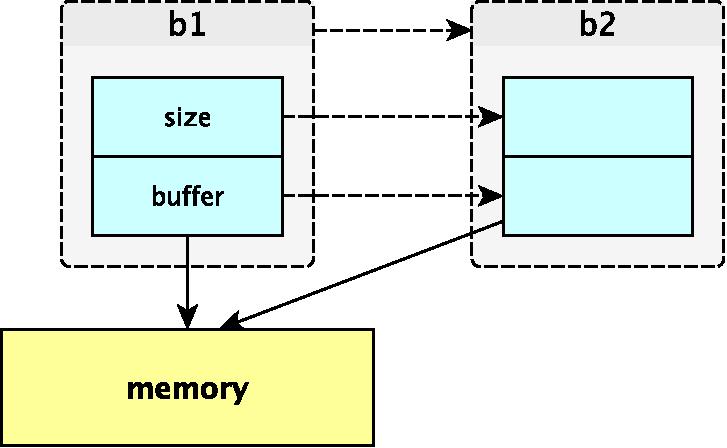
\includegraphics[width=0.6\textwidth]{illustrations/copying-crop.pdf}
\caption{Ошибка двойного освобождения}
\label{fig:copying-crop}
\end{figure}

Говорят, что по умолчанию C++ реализует поверхностное копирование (shallow copy\index{shallow copy}). Копирование с выделением нового буфера и копированием в него содержимого старого это глубокое копирование (deep copy\index{deep copy}) которое пользователь всегда должен реализовать самостоятельно. Ниже показано переопределение копирующего конструктора, о переопределении операторов и в частности оператора присваивания см. (\ref{OperatorOverloading})

\begin{lstlisting}
class CCopyableBuffer {
public:
  CCopyableBuffer(int size) : 
    m_size (size) m_buffer (new char[size]) {
  }
  ~CCopyableBuffer() { 
    delete[] m_buffer; 
  }
  CCopyableBuffer(const CCopyableBuffer& rhs) { 
    m_size = rhs.m_size; 
    m_buffer = new char[m_size];
    memcpy(m_buffer, rhs.m_buffer, m_size);
  } 
  char &get(int x) { 
     assert(x >= 0 && x < m_size); 
     return m_buffer[x]; 
  } 
private:
  char *m_buffer;
  int m_size;
};
\end{lstlisting}

Так всё будет работать. Но иногда копирование не нужно и его проще запретить, объявив собственные конструктор копирования и оператор присваивания в закрытой части класса.

\begin{lstlisting}
class NCBuffer {
public:
  NCBuffer(int size) : 
    m_size (size) m_buffer (new char[size]) {
  }
  ~NCBuffer() { 
    delete[] m_buffer; 
  }
  char &get(int x) { 
    assert(x >= 0 && x < m_size); 
    return m_buffer[x]; 
  }
private:
  char *m_buffer;
  int m_size;
  NCBuffer(const NCBuffer& rhs);
  NCBuffer& operator= (const NCBuffer& rhs);
};
\end{lstlisting}

Теперь компилятор не сгенерирует за вас неправильные варианты и копирование просто не будет скомпилировано.

Начиная с 2011 года, существует более цивилизованный способ запретить любой генерируемый по умолчанию метод или явно сгенерировать его -- ключевые слова \lstinline!default! и \lstinline!delete!.

\begin{lstlisting}
class NCBuffer {
public:
// .....
  NCBuffer(const NCBuffer& rhs) = delete;
  NCBuffer& operator= (const NCBuffer& rhs) = delete;
// .....
};
\end{lstlisting}

Человечное определение класса наподобие \lstinline!Empty!, которое не требует от программиста ``волшебных очков''.

\begin{lstlisting}
struct Empty {
  Empty() = default;
  ~Empty() = default;
  Empty(const Empty &rhs) = delete;
  Empty& operator=(const Empty &rhs) = delete;
};
\end{lstlisting}

\textbf{Домашняя наработка:} поясните или опровергните мысль: ``именно из-за проблемы двойного освобождения, в C++ нет и не может быть простого аналога realloc''

Конечно писать RAII-обертку на каждый ресурс это очень накладно (в англоязычной литературе любят использовать в таких случаях термин boilerplate code). Поэтому профессионалы пишут одну обертку на все типы ресурсов -- так называемые умные указатели, которые будут рассмотрены в (\ref{SmartPointers}).

\subsection{Оптимизации возвращаемого значения\index{RVO}}\label{RVO}

RVO или оптимизация возвращаемого значения, прописана в стандарт C++ (например 12.3.2.15 для C++98) и она гласит, если коротко, что компилятор имеет право не вызывать копирующие конструкторы если он может статически доказать, что объекты эквивалентны.

Пример:

\begin{lstlisting}
struct foo {
  foo () { cout << "foo::foo()" << endl; }
  foo (const foo&) { cout << "foo::foo( const foo& )" << endl; }
  ~foo () { cout << "foo::~foo()" << endl; }
};

foo bar() {
  foo local_foo;
  return local_foo;
}

int main() {
  foo f = bar();
  return 0;
}
\end{lstlisting}

В случае если GCC компилирует этот код без RVO (опция \lstinline!-fno-elide-constructors!), вывод на экран выглядит как:

\begin{lstlisting}
foo::foo()
foo::foo( const foo& )
foo::~foo()
foo::foo( const foo& )
foo::~foo()
foo::~foo()
\end{lstlisting}

Последовательность очевидна: создаётся локальный \lstinline!local_foo!, создаётся его копия -- возвращаемое значение, уничтожается \lstinline!local_foo!, возвращаемое значение копируется в \lstinline!f!, уничтожается возвращаемое значение, уничтожается \lstinline!f!.

В случае же обычной компиляции с RVO, вывод выглядит гораздо проще:

\begin{lstlisting}
foo::foo()
foo::~foo()
\end{lstlisting}

Эта экономия разрешена стандартом и поэтому программист не должен закладываться на то, что его конструктор копирования всегда будет вызван в контексте копирования.

\pagebreak
\section{Перегрузка\index{overload} операторов\index{operator}}\label{OperatorOverloading}

\hfill\textit{I left out operator overloading}

\hfill\textit{because I had seen too many people abuse it in C++}{\vspace{0.5em}}

\hfill\textit{-- James Gosling}

Язык C++ позволяет переопределять для пользовательских типов почти все операторы, которые применимы для встроенных типов, включая арифметические, логические, а также некоторые специального вида операторы. В прошлом разделе уже встречалось упоминание переопределения присваивания. Рассмотрим класс, абстрагирующий матрицу $N*M$ для $N>1, M>1$.

\textbf{Вопрос к студентам:} написать у доски то, что они уже знают: конструктор, деструктор, копирование, геттер/сеттер

\ifanswers
Возможный ответ:

\begin{lstlisting}
class Matrix
{
  int m_n, m_m;
  int *m_buf;
public:
  Matrix (int n, int m) : 
    m_n (n), m_m (m), m_buf (new int[n*m]()) {}
  ~Matrix () { delete [] m_buf; }

  Matrix (const Matrix &rhs) : 
    m_n (rhs.m_n), m_m (rhs.m_m), m_buf (new int[m_n * m_m]) {
      std::memcpy (m_buf, rhs.m_buf, 
                   rhs.m_n * rhs.m_m * sizeof(int));
  }

  Matrix &operator=(const Matrix &rhs) {
    Matrix tmp{rhs};
    m_n = tmp.m_n; m_m = tmp.m_m;
    std::swap(m_buf, tmp.m_buf);
    return *this;
  }

  void set (int x, int y, int val) { m_buf[x*m_m + y] = val; }
  int get (int x, int y) const { return m_buf[x*m_m + y]; }
};
\end{lstlisting}
\fi

Допустим, хотелось бы написать сложение матриц.

\begin{lstlisting}
Matrix& Matrix::addeq(const Matrix &rhs)
\end{lstlisting}

Использование очевидно.

\begin{lstlisting}
Matrix m, n;
// ....
m.addeq(n);
\end{lstlisting}

Но это не так красиво, как если бы допускалась более математическая запись с инфиксным сложением.

\begin{lstlisting}
m += n;
\end{lstlisting}

И C++, как вскоре станет ясно, даёт возможность переопределить операторы, такие как \lstinline!+!, \lstinline!=! и многие другие, чтобы добиться такой непосредственности в выражении мыслей.

Главная проблема здесь в том, что вы действительно вольны написать любой код в определении оператора сложения. Ваше сложение не обязано удовлетворять даже каким-то базовым инвариантам сложения:

\begin{lstlisting}
assert (a + b == b + a); /* ORLY? */
\end{lstlisting}

Вместо этого ваша операция сложения может осуществлять вычитание, лезть в базу данных или форматировать диск. Почти всегда, когда вы читаете код на C++, вы обязаны иметь в виду, что не можете быть уверены что значит операция \lstinline!+! этим утром. Ночью кто-нибудь мог вкоммитить в неё чудовищные изменения – из лучших побуждений, разумеется.

Всё усугубляется тем, что общий список операторов, которые можно переопределить, крайне внушающ. Его всегда можно посмотреть в стандарте, но кроме основных арифметических и логических операций, определение которых довольно таки прямолинейно, перегрузке могут подвергаться совершенно экзотические вещи – сравнение, присваивание, приведение к типу (любому, включая встроенные), обращение по указателю и даже выделение памяти с помощью new и её освобождение. Давайте побеседуем об нескольких специальных и проблематичных случаях переопределённых операторов.

\subsection{Операторы, формирующие цепочки}\label{ChainOps}

Первый особый случай, это операторы, которые могут быть записаны цепочками (обычно -- правоассоциативными). Скажем, пользователь оператора \lstinline!=!, скорее всего ожидает корректной работы строчки:

\begin{lstlisting}
x = y = z = w;
\end{lstlisting}

распространяющей, значение \lstinline!w! справа налево. Рассмотренный ранее (\ref{subsub:magicglasses}) буфер может и должен быть расширен определение оператора равенства, который для того, чтобы такая цепочка могла быть сформирована, должен возвращать ссылку на текущий объект

\begin{lstlisting}
CCopyableBuffer& operator=(const CCopyableBuffer& rhs){
  if (&rhs == this) return *this;
  delete [] m_buffer;
  m_size = rhs.m_size; m_buffer = new char[m_size];
  memcpy(m_buffer, rhs.m_buffer, m_size);
  return *this;
}
\end{lstlisting}

Особое внимание следует обратить на проверку \lstinline!if (&rhs == this)! в начале. Вторым способом написать эту проверку будет: \lstinline!if (rhs == *this)!

\textbf{Домашняя наработка:} почему второй способ может привести к некорректному и неожиданному поведению?

Большинство цепочечных операций: \lstinline!+=!, \lstinline!*=! и так далее, являются прямыми модификаторами состояния класса и должны быть определены в классе, чтобы у них был \lstinline!this! для возврата.

\subsection{Симметричные бинарные операторы}\label{SymmBinary}

Можно рассмотреть ещё один пример -- разработку класса, реализующего абстракцию комплексных чисел.

Для того, чтобы абстракция комплексных чисел была завершённой, должна быть возможность неявного преобразования double в complex, ведь по сути число \lstinline!2.0! это \lstinline!2.0 + 0.0 * i!. Эта возможность заложена в конструкторе класса (вспоминаем, что конструктор с одним аргументом это неявное преобразование типа).

\begin{lstlisting}
Complex a = Complex(1.0, 3.1), b;
b = a + 2.0; /* ok */
\end{lstlisting}

Но здесь таится и опасность, потому что сложение перестаёт быть коммутативным и простая запись, вида:

\begin{lstlisting}
Complex a = Complex(1.0, 3.1), b;
b = 2.0 + a; /* error! */
\end{lstlisting}

Выдаст ошибку компиляции. Ошибка связана с тем, что неявные преобразования применяются только к параметрам, перечисленным в списке параметров. Поэтому \lstinline!a.operator+(2.0)! преобразует \lstinline!double! к \lstinline!Complex!, но для \lstinline!(2.0).operator+(a)! неявный параметр \lstinline!this! -- указатель на объект для которого вызывается метод, не подвергается, согласно стандарту, никаким неявным преобразованиям.

Правильный метод: определить операторы сложения и умножения вне класса как отдельные функции. Очень часто бинарные операции проще всего определить в терминах цепочечных операций, определенных в классе.

\begin{lstlisting}
class Complex {
  double re, im;  
public:
  Complex(double r = 0.0, double i = 0.0) : re(r), im(i) {}

  double get_real() const { return re; }
  double get_imag() const { return im; }
  double operator+= (const Complex &rhs);
};

Complex operator+ (const Complex &lhs, const Complex &y) { 
  Complex tmp = lhs;
  tmp += rhs; // <----- call to operator +=
  return tmp;
}
\end{lstlisting}

Точно так же необходимо поступать со всеми функциями, которые по определению должны быть коммутативными. Тогда коммутативность будет сохранена.

На самом деле, можно сделать и иначе через friend функции, но это предпочтительный метод. Он кроме всего прочего позволяет естественным образом сохранить когерентность \lstinline!+! и \lstinline!+=! или в общем случае -- цепочечной и соответствующей ей бинарной операции.

\subsection{Инкремент и декремент}\label{IncrOverload}

Язык C++ получил своё название от унарной операции \lstinline!x++!, которая увеличивает значение переменной в данном случае x, и возвращает старое значение. Такая операция называется постинкрементом. Известен также прединкремент \lstinline!++x!, который увеличивает свой аргумент и возвращает увеличенное значение.

\begin{lstlisting}
Complex& Complex::operator++ () {
  re += 1.0;
  return *this;      
}
\end{lstlisting}

Такая запись возвращает прединкремент, он совсем простой. Постинкремент в терминах прединкремента может быть определен вот так:

\begin{lstlisting}
Complex operator++ (int unused) {
  Complex result = *this;
  ++(*this);
  return result;
} 
\end{lstlisting}

Очевидно, что прединкремент в общем случае не требует копирования, которое, как уже выяснилось, может быть очень дорогим. Поэтому очень часто программисты на C++ используют именно прединкремент в циклах:

\begin{lstlisting}
for (Complex t = 1.0; t < 5.0; ++t) { .... }
\end{lstlisting}

вместо

\begin{lstlisting}
for (Complex t = 1.0; t < 5.0; t++) { .... }
\end{lstlisting}

Обычно замеры показывают что такая запись не несет какого-то особого выигрыша. Она просто показывает, что человек знает внутреннюю механику языка.

\subsection{Вызов и индексация}\label{BracketOverloading}

Эта перегрузка позволяет объекту быть вызванным как функция (с круглыми скобками и передачей аргументов).

\begin{lstlisting}
class LessThan
{
public:
  explicit LessThan(int x = 0) : m_x(x) {}
  bool operator()(int y) const { return y < m_x; }
private:
  int m_x;
}
\end{lstlisting}

Определённый таким образом класс, позволяет иметь сразу несколько функцие-подобных объектов (также они называются \textbf{функторы}\index{Functor}), выражающих предикаты ``меньше x'' для разных \lstinline!x!.

\begin{lstlisting}
LessThan ltthree(3), ltfour(4), ltfive(5);

assert(ltthree(2));
assert(!ltthree(4));
\end{lstlisting}

И вызывать их по необходимости.

Аналогично возможно перегрузить операцию взятия индекса.

\begin{lstlisting}
struct TwoArray {
  int y, int z;
  int& operator[] (int x) {
    if (x == 0) return y;
    if (x == 1) return z;
    // error processing
  }
}
\end{lstlisting}

При использовании такого класса, синтаксис мало чем отличается от массивов

\begin{lstlisting}
TwoArray t;
t[0] = 1;
t[1] = 2;
assert (3 == t[0] + t[1]);
\end{lstlisting}

Если не знать, невозможно догадаться, что реально никакого массива никто не выделяет.

Переопределение квадратных скобок часто используется контейнерами стандартной библиотеки, в частности векторами и деками, см. (\ref{vectorarrs}).

\subsection{Разыменование и его варианты}\label{DereferenceOverloading}

Если есть классы, которые ведут себя как функции и массивы, логично предположить, что возможны классы, которые ведут себя как указатели. Для примера, можно рассмотреть так называемые умные указатели, о которых речь пойдет чуть дальше (см. \ref{SmartPointers}). Пусть есть несложная структура

\begin{lstlisting}
struct T {
  int x = 5;
  int foo () { return x; }
};
\end{lstlisting}

Можно изготовить класс, который будет вести себя почти как указатель на эту структуру

\begin{lstlisting}
class Tptr {
  T *t_;
public:
  Tptr(T *rhs) : t_(rhs) {};
  T operator*() const { return *t_; }
  T* operator->() const { return t_; }
};
\end{lstlisting}

В этом классе перегружены операторы обычного разыменования и разыменования с доступом к полю (часто для краткости его называют ``стрелкой''). Использование несложно.

\begin{lstlisting}
T t;
Tptr pt(&t);
pt->x = 6;
(*pt).foo();
\end{lstlisting}

Одной из важных особенностей перегрузки оператора стрелки является drill-down behaviour \index{Drill-Down behaviour} -- зарывающееся поведение: результат стрелки используется для разрешения имени, но если этого имени нет, то вместо него снова может быть выбран вызов стрелки.

\begin{lstlisting}
struct client { int a; };

struct proxy {
  client *target;
  client *operator->() const { return target; }
};

struct proxy2 {
  proxy *target;
  proxy &operator->() const { return * target; }
};

void f() {
  client x = { 42 };
  proxy y = { & x };
  proxy2 z = { & y };

  // prints 42 42 42
  printf ("%d %d %d\n", x.a, y->a, z->a);    
}
\end{lstlisting}

\textbf{Домашняя наработка:} в самой структуре \lstinline!T! теперь можно перегрузить \lstinline!operator&! который мог бы возвращать \lstinline!Tptr!, и таким образом, переписать код использования ещё проще. Попробуйте заставить это заработать.

В любом языке есть элементы бессмысленной джигитовки. В частности в C++ есть вызов по указателю на функцию:

\begin{lstlisting}
struct foo {
  int bar() { printf ("bar\n"); }
};

template <typename T>
void Apply (T* t, int (T::*bar)() ) {
  (t ->* bar) ();
}

int main () {
  int (foo::*pbar)() = &foo::bar;
  foo f;

  Apply (&f, pbar);

  return 0;
}
\end{lstlisting}

Скобки необходимы в \lstinline!Apply! поскольку приоритет \lstinline!->*! меньше, чем приоритет вызова функции.

Этот оператор тоже можно перегрузить. В перегрузке он самый неинтересный из всех операторов разыменования и ведет себя просто как произвольная бинарная операция. На самом деле он даже не обязан быть нестатическим!

Но помните: если вы обнаруживаете, что вы перегрузили \textbf{это}, значит у вас точно что-то пошло не так.

\subsection{Приведение типов}\label{CastOverloading}

Самый простой и в то же время самый богатый набор операторов это операторы приведения типов.

Для двух любых типов X и Y может быть четыре оператора приведения:

\begin{itemize}
\item Приведение Y к X, объявленное внутри X
\item Приведение X к Y, объявленное внутри Y
\item Приведение X к Y, объявленное внутри X
\item Приведение Y к X, объявленное внутри Y
\end{itemize}

При этом каждое приведение может быть явным или неявным.

Первые два вида это обычные конструкторы копирования. Пусть в качестве Y служит тип \lstinline!int! для простого примера, указатель на целое для чуть более сложного примера и (указатель на) массив из трёх целых для совсем сложного случая. Да, конечно, можно сказать, что нельзя придумать такой класс, который требовал бы неявного приведения к указателю на массив из трёх целых и обратно. Но я бы с этим поспорил.

\begin{lstlisting}
struct X 
{
  // converting ctor int -> X
  X(int) {}

  // converting ctor int* -> X
  X(int*) {}

  // converting ctor int(*)[3] -> X
  X(int(*)[3]) {}

  //implicit conversion
  operator int() const { return 7; }
 
  // explicit conversion
  explicit operator int*() const { return nullptr; }
 
  // Error: array operator not allowed in conversion-type-id
  // operator int(*)[3]() const { return nullptr; }

  // OK if done through typedef
  using arr_t = int[3];
  operator arr_t*() const { return nullptr; } 

  // Error: conversion to array not allowed in any case
  // operator arr_t () const; 
};
\end{lstlisting}
 
Использование довольно просто и поучительно

\begin{lstlisting}
int main() {
  // init ctor conversion
  X x(1);

  // again init ctor
  X x1 = 2;

  // again init ctor
  X x2 = static_cast<int>(3);
 
  int n = static_cast<int>(x); // OK, explicit
  int m = x;                   // OK, implicit
 
  int *p = static_cast<int*>(x); // OK, explicit
  int *q = x;                    // Fail: no implicit one
 
  int (*pa)[3] = x;  // OK
}
\end{lstlisting}

Всё это кажется довольно простым, но конкретную рекомендацию где написать какой конструктор всегда может дать только личный опыт.

\pagebreak
\section{Выделение и освобождение динамической памяти}\label{subsec:newdeleteredef}

В отличии от многих современных языков программирования, таких как Java, Python или Ruby, где работа с памятью скрыта от программиста, в языке C++ память это ресурс и тонкая настройка памяти это важный навык.

Ключевую роль в тонкой настройке памяти играет переопределение операторов выделения и освобождения памяти. Эта возможность -- нечто новое даже по сравнению с таким низкоуровневым языком как C, где, тем не менее, вся память почти безальтернативно приходит из единственной функции \lstinline!malloc!.

В C++ напротив, \lstinline!new! и \lstinline!delete! это операторы и в этом смысле они похожи на такие операторы как \lstinline!+! или \lstinline!-!, то есть являются чем-то, что можно переопределить.

В частности навык переопределения этих операторов понадобиться когда речь пойдёт о безопасности исключений (см. \ref{subsec:exceptions}) и о пользовательских аллокаторах (см. \ref{allocators}).

\subsection{Глобальные операторы}\label{subsub:globalnew}

Самым близким аналогом функций \lstinline!malloc! и \lstinline!free! являются глобальные операторы \lstinline!::operator new! и \lstinline!::operator delete!. Они используются каждый раз когда в классе не переопределёны \lstinline!new! и \lstinline!delete! либо для встроенных типов.

Очень часто они напрямую реализованы через механизмы языка C, так что начинающему программисту кажется, что отличий нет. Тем не менее,, отличий довольно много.

Функции \lstinline!malloc! и \lstinline!free! отличаются тем, что:

\begin{enumerate}
\item
Память аллоцируется из кучи (``Heap'')
\item
Возвращаемое значение имеет тип \lstinline!void*!
\item
При неудаче \lstinline!malloc! возвращает \lstinline!NULL!
\item
Требуют спецификации точного размера в байтах
\item
Выделение массива требует ручного подсчёта места на массив
\item
Перевыделение памяти просто (нет вызова копирующих конструкторов)
\item
Никогда не вызовут из себя \lstinline!new! или \lstinline!delete!
\item
Нет способа автоматически побить запрашиваемую память на более мелкие участки при нехватке памяти на большой линейный кусок
\item
Не могут быть легально переопределены ни в каком случае
\end{enumerate}

В отличие от них, \lstinline!::operator new! и \lstinline!::operator delete! имеют следующие свойства:

\begin{enumerate}
\item
Память аллоцируется из свободного хранилища (``Free Store''). Совпадает ли оно с кучей (``Heap'') упомянутой выше или это два разных места -- зависит от реализации. Обычно в Unix совпадает, так как используется системный вызов sbrk, но есть варианты.
\item
Возращаемое значение -- типизированный указатель
\item
Обычно выбрасывает исключения при неудаче (см. ниже про специальные формы)
\item
Размер памяти вычисляется компилятором исходя из данного типа
\item
Есть версия специально для массивов
\item
Перевыделение памяти сложно (из-за вызова конструкторов) и нет его стандартной поддержки (аналога realloc)
\item
Вызовут ли они из себя \lstinline!malloc! или \lstinline!free! зависит от реализации
\item
Поддерживают установку аллокатора для случая исчерпания памяти через \lstinline!set_new_handler!
\item
Могут быть легально переопределены для пользовательских типов
\item
Используют конструкторы для инициализации объектов и деструкторы для освобождения их ресурсов
\end{enumerate}

\subsection{Стандартные и специальные формы new}\label{subsub:placementnew}

Рассмотрим типичное выделение памяти в программе на C++:

\begin{lstlisting}
class Widget {};
...
Widget *w = new Widget;
\end{lstlisting}

Предположим, оператор \lstinline!new! не переопределён для класса \lstinline!Widget!

Что здесь происходит? Неожиданно много всего.

\begin{enumerate}
\item
Сначала, по форме оператора new, компилятор определяет какой именно new имеется в виду. Существуют три нормальные формы new:
\begin{itemize}
\item
\lstinline!new! в куче с возбуждением исключений при исчерпании памяти. Именно он использован в рассматриваемом примере.
\item
\lstinline!new! в куче с возвратом нуля при исчерпании памяти
\item
placement new (размещающий \lstinline!new!)\index{placement new} (с размещением в заданном месте). Именно он и был использован в листинге выше. Его синтаксис похож на выделяющий new из этого примера, но буфер, в котором размещается сконструированный объект, не выделяется, а передаётся как параметр в скобках.
\end{itemize}

Кроме нормальных существуют ещё и специальные формы new, когда пользователь некоего типа переопределяет размещающий new этого типа передавая ему не область памяти, а нечто иное -- скажем область памяти и поток для записи лога и т.п. В следующем листинге показано использование разных форм new.

\begin{lstlisting}
class Widget {};
...
Widget *w = new Widget;
Widget *w = new (std::nothrow) Widget;
Widget *w = new (WidgetPool) Widget;
Widget *w = new (WidgetPool, WidgetLogStream) Widget;
\end{lstlisting}

Здесь первая строчка это выделение памяти с возбуждением исключения при ошибке выделения и вызов конструктора. Вторая строчка это выделение памяти без возбуждения исключения при ошибки выделения (тогда в \lstinline!w! просто запишется нулевой указатель). Третья строчка это просто вызов конструктора на уже выделенную память (при этом неудачи выделения быть, разумеется, уже не может). И четвёртая строчка иллюстрирует специальную пользовательскую форму оператора \lstinline!new! и не будет скомпилирована, без специальных объявлений внутри класса \lstinline!Widget!.

\item
Далее компилятор выделяет память в куче (строго при необходимости, размещающие и специальные формы пропускают этот пункт) и в случае нехватки памяти вызывает пользовательский обработчик, который можно поставить и на стандартное выделение с помощью \lstinline!set_new_handler!.
\item
Далее в случае если вызвана нормальная форма неразмещающего new, компилятор вызывает конструктор размещённого в куче объекта или все конструкторы, если был размещён массив.
\item
Разрушение происходит в обратном порядке.
\end{enumerate}

Обычный сценарий работы \lstinline!malloc()! для выделения буфера, вместе с размещающим \lstinline!new! для явного вызова конструктора приведён ниже:

\begin{lstlisting}
class Widget {
  int m_i;
public:
  Widget(int a_i): m_i(a_i * a_i) {}
  int get_state() const  { return m_i; }
  ~Widget() {}
};
\end{lstlisting}

\begin{lstlisting}
Widget *test_malloced(int initializer) {
  Widget *wbuf = (Widget *) malloc(sizeof(Widget));
  Widget *w = new (wbuf) Widget(initializer);
  return w;
}
\end{lstlisting}

\begin{lstlisting}
int main() {
  Widget *w = test_malloced(5);
  assert(w->get_state() == 25);
  w->~Widget();
  free(w);
  return 0;
}
\end{lstlisting}

Обратите внимание -- деструктор может быть вызван явно.

\subsection{Список нормальных форм}\label{subsub:normalforms}

Ниже приведен класс для которого объявлены переопределения всех нормальных форм \lstinline!new!/\lstinline!delete! как это сделано в \cite{effcpp3d}.

\begin{lstlisting}
struct StandardNewDeleteForms {
  static void *operator new(std::size_t size);
  static void operator delete(void * memory);
  static void *operator new(std::size_t size, const std::nothrow_t &nt);
  static void *operator new(std::size_t size, void *ptr);
};
\end{lstlisting}

\textbf{Домашняя наработка:} Напишите и протестируйте код для каждого из переопределений.

\pagebreak
\section{Правые ссылки и семантика перемещения}

\hfill\textit{If you take a reference to a reference to a type,}

\hfill\textit{you get a reference to that type,}

\hfill\textit{rather than some kind of special reference to reference type.} {\vspace{0.5em}}

\hfill\textit{-- Bjarne Stroustrup}

Ссылки (references) это то, что наиболее сложно воспринимается при переходе с C на C++. Человеку с опытом программирования на C, может быть непонятно, зачем они нужны, когда уже есть такие удобные и привычные указатели, которые позволяют делать всё то же самое только лучше... Подлинное осознание того, каким именно инструментом являются ссылки и как ими оперируют, приходит с опытом C++. При переходе на новый стандарт C++11, идея о том, что теперь есть ещё один вид ссылок -- ссылки на rvalue (rvalue references) кажется новаторской и неочевидной (особенно неочевидна её полезность). Скорее всего, многим придётся преодолеть внутреннее сопротивление, прежде чем rvalue references станут удобным и привычным инструментом. 

\subsection{Правые и левые значения}\label{LRvaluesAgain}

Прежде, чем переходить к описанию rvalue references, есть смысл немного вспомнить о том, что такое rvalue и lvalue.

Термин lvalue был, прежде чем перейти в C++, документально зафиксирован в стандарте языка C, поэтому логично начать изложение с него. Для языка C, lvalue (от left hand side value) -- то, что может появиться слева в выражении присваивания. Формально (6.3.2.1 стандарта C99), ``An lvalue is an expression with an object type or an incomplete type other than void'' (под object type в стандарте понимаются все типы, не являющиеся function type или incomplete type).

\begin{lstlisting}
int c = a * b; // ok, c is lvalue
a * b = 42;    // fail, a*b is rvalue
foo() = 42;    // fail in C, foo() is rvalue
\end{lstlisting}

Собственно, в стандарте языка C90 и последовавшем за ним C99 нет термина rvalue. В C99 есть оговорка ``What is sometimes called ``rvalue'' is in this International Standard described as the ``value of an expression'''', позволяющая предположить, что к этому времени этот термин существовал и использовался, но фиксировать его строго в случае языка C было не нужно.

Всё изменилось с приходом языка C++, который принёс с собой ссылки (lvalue references). Выражение из прошлого примера:

\begin{lstlisting}
foo() = 42; // in C++ this might be ok
\end{lstlisting}

может быть ошибкой если foo возвращает значение, но совершенно корректно, если foo возвращает ссылку. Чтобы разрешить эту неоднозначность, стандарт C++98 объявляет (3.10.1) два термина -- lvalue и rvalue, причём каждое выражение языка C++98 является либо тем, либо другим. При этом определение в (3.10.2) гласило ``An lvalue refers to an object or function''.

То есть lvalue это не первоклассный объект как в C, а просто некое выражение ссылающееся на область памяти. Таким образом в качестве главного различия выступает возможность взять адрес, а не отношение к операции равенства.

\begin{lstlisting}
int& foo();
foo() = 42;        // ok
int* p1 = &foo();  // ok
int foobar();
int* p2 = &foobar(); // fail
\end{lstlisting}

Таким образом, lvalue в C++98 приобретает смысл locator value (а не left hand side value). Так, например если есть \lstinline!int *val!, то выражение \lstinline!val+1! можно разыменовать, но нельзя взять его адрес.

\begin{lstlisting}
int *val;
int correct = *(val + 1); // ok
int **wrong = &(val + 1); // fail
\end{lstlisting}

При этом в качестве двух облачков на горизонте языка маячили проблемы семантики перемещения и проброса аргументов. Пока что эти слова достаточно упомянуть, смысл они приобретут чуть ниже по тексту. Оказалось, что обе проблемы имеют красивое решение, если дополнить язык ссылками на rvalues, также называемыми rvalue references или правыми ссылками.

\subsection{Ссылочное связывание}\label{subsub:refbinding}

Связыванием (binding) называется сопоставление ссылки как альтернативного имени реальному содержимому памяти. Даже очень простые случаи связывания могут вызывать некоторое удивление.

\begin{lstlisting}
int x = 1;
int &a = x;
int const &b = x;
int const &c = x + 1;
x = a + b + c;
cout << a << b << c;  // 4 4 2
\end{lstlisting}

Многих удивляет, что здесь на экране 4 4 2, а не 4 4 5. Вроде бы ссылка \lstinline!c! связана со значением \lstinline!x+1!. Но что произошло на самом деле -- ссылка \lstinline!c! была связана с временным объектом и автоматически продлила время его жизни. Важно, что для левых ссылок так работают только константные левые ссылки и получившийся временный объект является неизменяемым без специальных хаков.

Правую (неконстантную) ссылку в её базовом виде можно считать способом связаться с изменяемым временным объектом.

\begin{lstlisting}
int x = 1;
int &a = x;
int const &c = x + 1;
int &&d = x + 1;
c += 1; // fail
d += 1; // ok
\end{lstlisting}

Таким образом, в этом фрагменте кода \lstinline!d! работает как ссылка на rvalue -- неименованное изменяемое значение.

Несколько простых правил относительно взаимодействия и кросс-связывания ссылок изложено ниже.

\begin{enumerate}
\item
Правая ссылка не может быть связана с lvalue
\begin{lstlisting}
int x = 1; 
int &&y = x * 3; // ok
int &&b = x; // fail, not rvalue 
\end{lstlisting}
\item
Неконстантная левая ссылка не может быть связана с rvalue
\begin{lstlisting}
int &c = x * 3; // fail, not lvalue
const int &d = x * 3; // ok, extends lifetime
\end{lstlisting}
\item
Но при этом правая ссылка сама по себе задаёт имя и адрес и является lvalue
\begin{lstlisting}
int &&e = y; // fail, not rvalue
int &f = e; // ok, rvref is lvalue
\end{lstlisting}
\end{enumerate}

Функция может быть перегружена по типу ссылки

\begin{lstlisting}
int foo (int &p); // 1
int foo (int &&p); // 2
int x = 1;
foo (x); // 1
foo (x + 0); // 2
foo (foo (x)); // 1, then 2
\end{lstlisting}

Методы у класса могут зависеть от того является ли объект класса левым или правым значением (так же, как они различаются по cv-квалификаторам).

\begin{lstlisting}
struct S {
  int foo () &; // 1
  int foo () &&; // 2
};
extern S bar ();
S x {};
x.foo(); // 1
bar().foo(); // 2
\end{lstlisting}

\textbf{Вопрос студентам:} продление времени жизни левыми константными ссылками вызывает интересные проблемы.

\begin{lstlisting}
struct Base {};
struct Derived : public Base {};

Derived __attribute__ ((noinline))
derivedret ()
{
  return Derived ();
}

void
tricky_1 ()
{
  const Base &corr = derivedret ();
  /* use corr */
} /* which destructor? */
\end{lstlisting}

Какой деструктор будет вызван в этом случае? 

\ifanswers
Правильный ответ: Оказывается статический тип временного объекта известен компилятору и будет вызван деструктор класса \lstinline!Derived!. То есть ссылки не требуют виртуальных деструкторов для своей диспетчеризации -- компилятор сам может построить верный код удаления.
\fi

Теперь пришло время более интересного трюка: что если хочется связать правую ссылку со значением существующего объекта? Для этого нужно анонимизировать этот объект, превратить его в безликое значение. Традиционно для этого применяется стандартная функция \lstinline!std::move!

\begin{lstlisting}
int x = 42;
int &&rvx = std::move(x);
rvx += 2; 
assert(x == 44);
\end{lstlisting}

Понимание того как живут rvalue references и временные объекты, позволяет использовать класс, сочетающий левые и правые ссылки:

\begin{lstlisting}
struct RefBind
{
  int& ref;

  RefBind(int&& r) : ref(r) {}

  RefBind const& plus(int x) const { ref += x; return *this; }
  RefBind const& mult(int x) const { ref *= x; return *this; }

  int get() const { return ref; }
};
\end{lstlisting}

Три сценария использования:

\begin{lstlisting}
  int x = 1;

  std::cout << RefBind(1).plus(2).mult(3).get() << std::endl;
  std::cout << RefBind(std::move(x)).plus(2).mult(3).get() << std::endl;
  std::cout << RefBind(int(x)).plus(2).mult(3).get() << std::endl;
\end{lstlisting}

Первая строчка работает с чисто временным объектом, привязанным к lvalue ссылке и поэтому модифицируемым. Вторая попутно изменяет значение переменной \lstinline!x!, третья делает из переменной временный объект и работает с ним.

Можно сказать, что \lstinline!move! приводит объект к правой ссылке.

Можно ли привести объект к иной ссылке? Да, но с проблемами. Для этого в языке вроде как есть похожие функции \lstinline!std::ref! и \lstinline!std::cref!. Но именно, что вроде как есть, потому что на самом деле они работают совершенно иначе.

\begin{lstlisting}
int x = 1;
int &&a = move(x);
int &b = ref(x); 
const int &c = cref(x);
\end{lstlisting}

С виду всё то же самое, но это симметрия обманчива, так как \lstinline!std::ref! коварен:

\begin{lstlisting}
auto f = move(x); // -> int&&
auto e = ref(x); // -> std::reference_wrapper<int> 
\end{lstlisting}

Ссылочное связывание, разумеется, задаёт уровень косвенности и эта связь может стать некорректной.

\subsection{Провисание ссылок}\label{subsub:danglingrefs}

Проблема висячих ссылок (dangling references) известна давно и каждому программисту. Для левых ссылок она была рассмотрена ранее в (\ref{DanglingRefs})

\begin{lstlisting}
void simple_dangle ()
{
  int *myArray;
  myArray = new int[2]{ 100, 200 };
  int& ref = myArray[0];
  delete[] myArray;
  cout << "100 = " << ref << endl;  // dangling reference  
}
\end{lstlisting}

Ссылка на что угодно, время жизни чего истекло это висячая ссылка. Но такие вещи программисты обычно отлавливают (сами или инструментально) и контролируют. Гораздо хуже, если ссылка провисает в результате ссылочного связывания при возвращении из функции.

Ниже приведено несколько примеров.

\begin{itemize}
\item
\begin{lstlisting}
const int& 
clref (int p) { return p + 0; } // p+0 is dead
\end{lstlisting}
Константная левая ссылка связана со временным значением
\item
\begin{lstlisting}
const int& 
clref (int p) { return p; } // p rests in peace 
\end{lstlisting}
Не смотря на внешние различия, также константная левая ссылка связана со временным значением
\item
\begin{lstlisting}
int& 
lref (int p) {  return p; } // p is p no more
\end{lstlisting}
Левая ссылка опять (сюрприз) связана с истекшим временным значением
\item
\begin{lstlisting}
int&& 
rref (int p) { return p + 0; } // p+0 expired and gone 
\end{lstlisting}
Правая ссылка связана с истекшим временным значением. Получается странная вещь: висячая правая ссылка.
\item
\begin{lstlisting}
int&& 
rvref (int &&p) { return p + 0; } // p+0 is an ex-p+0
\end{lstlisting}
Несмотря ни на что, снова правая ссылка связана со временным значением
\end{itemize}

На этом фоне всеобщего уныния, есть несколько на удивление работающих конструкций. 

\begin{itemize}
\item
\begin{lstlisting}
int& 
lvref (int &x) { return x; } // ok
\end{lstlisting}
Константная левая ссылка связана со временным значением
\item
\begin{lstlisting}
const int& 
clvref (const int &x) { return x; } // also ok
\end{lstlisting}
\end{itemize}

Их общим признаком является тот факт, что идентичность объекта под ссылкой сохраняется в вызывающем фрейме.

\textbf{Вопрос к студентам:} что будет если попытаться использовать значение объекта типа \lstinline!RefBind! (код для этого типа приведён в \ref{subsub:refbinding}) после конца полного выражения?

\begin{lstlisting}
RefBind x(1);
cout << x << endl;
\end{lstlisting}

\ifanswers
Правильный ответ: dangling rvalue reference.
\fi

\subsection{Семантика перемещения}\label{subsub:movesemantics}

Первая серьёзная проблема, решение которой было обещано в начале раздела, это проблема семантического выражения перемещения. Она может быть проиллюстрирована проблемой COAP (см. \ref{COAP}) -- действительно контейнеры из \lstinline!auto_ptr! вели себя странно, потому что перемещение и копирование никак не были разделены: в языке была возможность написать \lstinline!a = b! но не \lstinline!move(a,b)! и заложенная в переопределенный оператор присваивания семантика перемещения оказалась миной: рано или поздно так или иначе кто-то все равно использует присваивание как присваивание.

С помощью правых ссылок, список специальных методов класса (уже включающий конструкторы, копирующие конструкторы, операторы присваивания и т.д.) был дополнен ещё двумя -- перемещающими конструкторами и перемещающим присваиванием.

Перемещающий конструктор выглядит очень похоже на копирующий, но берёт правую ссылку.

\begin{lstlisting}
class Buffer {
  size_t sz; int *buf;
public:
  Buffer (Buffer&& rhs) : sz(rhs.sz), buf(rhs.buf) { 
    rhs.sz = 0; rhs.buf = nullptr; 
  }
  Buffer (const Buffer& rhs) : sz(rhs.sz), buf(new int[sz]) { 
    copy (rhs.buf, rhs.buf + sz, buf); 
  }
};
\end{lstlisting}

Если предположить, что упомянутый в листинге класс буфера содержит большое количество тяжёлых данных, видно, что перемещение выглядит куда дешевле, чем копирование.

В свете перемещающих конструкторов особенно важным становится правило, что правая ссылка это lvalue. Легко представить ситуацию, в которой в наследуемом от \lstinline!Buffer! классе \lstinline!DerivedBuf!, есть необходимость эти конструкторы переопределить. С первого взгляда можно сделать это следующим образом:

\begin{lstlisting}
DerivedBuf(DerivedBuf const & rhs) : Buffer(rhs) {};
DerivedBuf(DerivedBuf&& rhs) : Buffer(rhs) {}; // FAIL
\end{lstlisting}

Перемещающий конструктор переопределён неверно -- поскольку \lstinline!rhs! имеет имя, оно является lvalue, а значит \lstinline!DerivedBuf(rhs)! в данном случае вызовет снова \lstinline!Buffer(Base const & rhs)!, что, вероятно, не желательно. Вместо этого следует писать

\begin{lstlisting}
DerivedBuf(DerivedBuf&& rhs) : Buffer(std::move(rhs)) {};
\end{lstlisting}

Говорят, что \lstinline!std::move! скрывает имя \lstinline!rhs!, делая его таким же безымянным rvalue выражением, как \lstinline!a*b!. Это общее правило ``оно не должно иметь имени'' очень полезно для выработки интуиции.

Аналогично перемещающему конструктору работает перемещающее присваивание

\begin{lstlisting}
Buffer& operator= (Buffer&& rhs) {
  if (this == &rhs) 
    return *this;
  delete [] buf;
  sz = rhs.sz;
  buf = rhs.buf;
  rhs.sz = 0;
  rhs.buf = nullptr;
  return *this;
} 
\end{lstlisting}

Хороший (но не самый простой) способ показать где это нужно это рассмотреть возврат из функции по значению

\begin{lstlisting}
Buffer foo () {
  Buffer retval;
  // filling retval
  return retval;
}

Buffer t = foo(); // t move-constructed, not copied
\end{lstlisting}

Серьёзная ошибка это писать явный \lstinline!move! внутри \lstinline!return!. Это может привести к подвисанию ссылки. 

Дополнительная красота этого примера в том, что не написав там ни одной правой ссылки, программист, тем не менее, активно пользуется правыми ссылками в неявном виде.

Ещё один (и пожалуй простейший) способ показать где годятся новые специальные методы это рассмотреть функцию обмена значениями (так поступают почти все известные автору источники, потому что пример уж больно нагляден).

Старый способ обмена значениями (до 2011 года)

\begin{lstlisting}
template <typename T> void swap (T& x, T& y) {
  T tmp = x; // copy ctor
  x = y; // assign
  y = tmp; // assign
} 
\end{lstlisting}

Новый способ очевидно лучше (представьте вместо \lstinline!T! класс \lstinline!Buffer!).

\begin{lstlisting}
template <typename T> void swap (T& x, T& y) {
  T tmp = move(x); // move ctor
  x = move(y); // move assign
  y = move(tmp); // move assign
} 
\end{lstlisting}

Этот код во многом вводит новичка в искушение. При взгляде на него кажется, что использование move само по себе действительно что-то куда-то перемещает. Вряд ли можно придумать худшее заблуждение. Кое-что, конечно перемещается, но по другой причине. Это можно проиллюстрировать следующшим кодом (обратите внимание на asserts ниже).

\begin{lstlisting}
int x = 1;
int a = move(x);
assert (x == a); // always ok
Buffer y {10};
Buffer b = move(y);
assert (y == b); // always failed
\end{lstlisting}

Идея в следующем: просто move всего лишь анонимизирует переменную ничего с ней не делая. Будет ли состояние потеряно зависит от того есть ли у класса move-конструктор и как он реализован. У int его точно нет, на чём и построен первый ответ.

Именно с тем, что настоящее перемещение делает не язык, не компилятор (они всего лишь обеспечивают move специальной семантикой) а сам программист, программист может и выстрелить себе в ногу.

\begin{lstlisting}
class SillyBuffer {
  int sz; int *buf;
public:
  SillyBuffer (int s = 10): sz(s), buf(new int[sz]){}
  ~SillyBuffer () { delete [] buf; }
};
void swap (SillyBuffer& lhs, SillyBuffer& rhs) {
  SillyBuffer tmp = move (lhs);
  lhs = move (rhs);
  rhs = move (tmp);
} // UB (probably segfault) 
\end{lstlisting}

Перемещение по умолчанию перемещает по умолчанию все поля класса. Перемещая по умолчанию указатель оно побитово его копирует. После этого столь глупое перемещение будет вести себя не лучше, чем копирование по умолчанию для того же класса.

Классическая идиома проектирования rule of five утверждает, что если ваш класс требует нетривиального определения хотя бы одного из пяти методов:

\begin{itemize} 
\item копирующего конструктора
\item копирующего присваивания,
\item перемещающего конструктора
\item перемещающего присваивания 
\item деструктора
\end{itemize} 

то вам лучше бы нетривиально определить все пять

Очевидно \lstinline!SillyBuffer! его нарушает: он определяет нетривиальный деструктор и только его.

Итак, хорошо организованный move ctor изменяет rhs. Но что если rhs нельзя изменить?

\begin{lstlisting}
const Buffer y {10};
Buffer b = move(y);
assert (y == b); 
\end{lstlisting}

В этом случае move ctor просто не будет вызван, так как его сигнатура предполагает \lstinline!Buffer &&! а не \lstinline!Buffer const &&!.

Вместо этого, \lstinline!Buffer const &&! будет приведён к \lstinline!Buffer const &! и вызовется копирующий конструктор, несмотря на явное указание \lstinline!move!.

Таблица специальных методов подытоживает этот раздел (теперь вы знаете достаточно, чтобы понимать здесь каждую строчку). Любой специальный метод, не объявленный пользователем, может быть объявлен по умолчанию (def), отсутствовать (none) или стёрт (del). Крестики стоят там, где строка, соответствующая методу объявленному пользователем, совпадает со столбцом, где перечислены неявные методы.

\begin{center}
  \begin{tabular}{ | c | p{1cm} | p{1cm} | p{1cm} | p{1cm} | p{1cm} | p{1cm} | }
    \hline
     & default ctor & dtor & copy ctor & copy assign & move ctor & move assign \\ \hline \hline
    Nothing & def & def & def & def & def & def \\ \hline
    Any ctor & none & def & def & def & def & def \\ \hline
    Default ctor & x & def & def & def & def & def \\ \hline
    Dtor & def & x & def & def & none & none \\ \hline
    Copy ctor & none & def & x & def & none & none \\ \hline
    Copy assign & def & def & def & x & none & none \\ \hline
    Move ctor & none & def & del & del & x & none \\ \hline
    Move assign & def & def & del & del & none & x \\ \hline
  \end{tabular}
\end{center}

Конечно, главная проблема здесь в обратной совместимости с C++98 в том, что касается копирования и присваивания по умолчанию даже если пользователь определил только один из этих двух методов. Это был суровый просчёт в проектировании и сколько лет ещё с ним жить -- не очень понятно. Благо к этим конкретным граблям все давно привыкли.

Здесь заканчивается тонкая настройка ``волшебных очков'' выданных ранее в (\ref{subsub:magicglasses}). Теперь через них видно всё.

\textbf{Вопрос студентам:} какую из двух предложенных сигнатур вы выберете и почему?

\begin{lstlisting}
vector<string> create_vector_of_strings(); // 1
create_vector_of_strings(vector<string>&); // 2
\end{lstlisting}

\ifanswers
Правильный ответ: их более одного. Всё изложение подталкивает к ответу (1), но тут возможен спор. В любом случае этот спор нужно вести с учётом конструкторов перемещения. Аргументировать (2) тут гораздо сложнее, но на практике-то все пишут именно так.
\fi

Итак, rvalue references позволяют (совместно с \lstinline!std::move!) по новому взглянуть на ссылки и открывают простор к более тонкому различию таких терминов естественного языка как ``копирование'', ``присваивание значения'', ``присваивание результата'' на языке C++, что открывает как простор к оптимизациям, так и возможности более аккуратного выражения старых идиом (хороший пример блестящего использования правых ссылок это \lstinline!std::unique_ptr! который в новом стандарте пришёл на смену печально известному \lstinline!auto_ptr!). 

\begin{lstlisting}
  auto_ptr <int> told (new int(2));
  auto_ptr <int> sold (new int(3));

  told = sold;

  unique_ptr <int> t (new int(2));
  unique_ptr <int> s (new int(3));

  // t = s; -- compilation error, no copy ctor
  t = std::move (s); // -- ok, move ctor
\end{lstlisting}

Здесь правило большой пятерки вовсе не нарушено -- копирующее присваивание в \lstinline!unique_ptr! сознательно запрещено через \lstinline!=delete!, а это вполне нетривиальное определение. Больше про умные указатели нового стандарта см. (\ref{SmartPointers}).

Это закрывает первый вопрос и теперь настало время поговорить о втором, но сначала необходимо узнать больше про правила работы с правыми и левыми ссылками.

\subsection{Свёртка ссылок}\label{ReferenceConvolution}

Два вида ссылок дают возможность развернуться с записью ссылок на ссылки на ссылки. Простейший случай вывода типов уже ставит соответсвующие проблемы.

\begin{lstlisting}
int x;
int &y = x;
auto &&c = y; // -> yields what?
\end{lstlisting}

Уточнённое с помощью rvalue reference, auto не может игнорировать ссылку
Формально вывод выглядит так:

\begin{lstlisting}
auto &&c = y; // -> int & && c = y;
auto &&d = move(y); // -> int && && c = y;
\end{lstlisting}

Чтобы получился корректный тип, ссылки должны быть свёрнуты (collapsed).

Стандарт C++11 (8.3.2.6) определяет следующие правила свёртки ссылок, применимые для определений \lstinline!auto! и \lstinline!decltype!, \lstinline!typedef!, а также параметров шаблонов:

\lstinline!A& &! становится \lstinline!A&!
\lstinline!A& &&! становится \lstinline!A&!
\lstinline!A&& &! становится \lstinline!A&!
\lstinline!A&& &&! становится \lstinline!A&&!

Говоря коротко, левая ссылка выигрывает там, где она есть. Для рассмотренного выше примера это даёт:

\begin{lstlisting}
auto &&c = y; // -> int & && c -> int &c = y;
auto &&d = move(y); // -> int && && d 
                    // -> int &&d = move(y);
\end{lstlisting}

Правила вывода дают интересную картину: \lstinline!auto&! это всегда lvalue ref, но \lstinline!auto&&! это либо lvalue ref, либо rvalue ref (зависит от контекста)

\begin{lstlisting}
auto &&y = x; // x это some& -> y это some&
\end{lstlisting}

Это в целом работает и для decltype

\begin{lstlisting}
decltype(x) && z = x; // the same
\end{lstlisting}

И для шаблонов

\begin{lstlisting}
template <typename T> void foo(T&& t);
foo(x); // the same
\end{lstlisting}

Такие ссылки называют forwarding references. Майерс \cite{effmoderncpp} предложил называть их универсальными ссылками. По русски ``универсальные'' звучит лучше, чем ``пробросовые'' поэтому неформальный термин Майерса я буду употреблять чаще.

Важно отличать настоящие универсальные ссылки от фальшивых (от последних никакой радости).

Контекст сворачивания требует вывода типов, а не их подстановки:

\begin{lstlisting}
template<typename T> struct Buffer {
  void emplace (T&& param);  // T is substituted
.....
};
\end{lstlisting}

В примере выше параметр известен в момент инстанцирования класса и просто подставляется в метод. Это правая ссылка, никакого сворачивания тут нет. А вот в примере ниже оно появляется.

\begin{lstlisting}
template<typename T> struct Buffer {
  template<typename U>
  void emplace (U&& param);  // U is inferred and collapsed
.....
};
\end{lstlisting}

Контекст для сворачивания не будет создан, если тип уточнён более, чем \lstinline!&&!

\begin{lstlisting}
template<typename T> void buz (const T&& param); 
\end{lstlisting}

Это так же верно для auto

\begin{lstlisting}
const auto &&x = y;  // rvalue ref 
\end{lstlisting}

\subsection{Пробрасывание, близкое к совершенству}\label{PerfectForw}

Название perfect forwarding несколько излишне амбициозно. Я предпочитаю переводить его на русский язык, как ``проброс, близкий к совершенству''. Постановка проблемы следующая: некая функция принимает аргумент и должна, ничего с ним не сделав, передать его как аргумент другой функции. При этом если аргумент изначально был rvalue, он должен придти как rvalue, а если он был lvalue, то как lvalue. Это и есть вторая серьёзная проблема из заголовка. Полностью совершенным этот проброс назвать нельзя, так как категорий значений на самом деле не две, а пять (см. дальше) но по условию задачи должны сохраняться только две (реально сохраняются четыре).

Чтобы проиллюстрировать актуальность, можно рассмотреть прозрачную оболочку (первое приближение см. transparent в разделе \ref{DecltypeAuto14}).

\begin{lstlisting}
template <typename Fun, typename Arg> decltype(auto)
transparent (Fun fun, Arg arg) { 
  return fun(arg); 
}
\end{lstlisting}

Увы, её недостаток в том, что она не слишком прозрачна. Например следующий код очевидно порождает лишнее копирование при создании временной переменной для формального параметра.

\begin{lstlisting}
extern Buffer foo (Buffer x);
Buffer b;
Buffer t = transparent (&foo, b); // copy b
\end{lstlisting}

Возможный выход: уточнить аргумент ссылкой. Пока непонятно какая подойдёт лучше, но с примером выше будет работать левая, так что можно попробовать левой.

\begin{lstlisting}
template <typename Fun, typename Arg> decltype(auto)
transparent (Fun fun, Arg& arg) {
  return fun(arg); 
}
\end{lstlisting}

Теперь лишнего копирования для rvalues вроде бы нет. Но появляется новая беда: теперь rvalues не проходят в функцию.

\begin{lstlisting}
extern Buffer foo (Buffer x);
Buffer b;
Buffer t = transparent (&foo, b); // ok
Buffer u = transparent (&foo, foo(b)); // fail, CE
\end{lstlisting}

И действительно, левая ссылка не может быть связана с rvalue. Возможный выход: перегрузить по константной ссылке.

\begin{lstlisting}
template <typename Fun, typename Arg> decltype(auto)
transparent (Fun fun, Arg& arg) { return fun(arg); }

template <typename Fun, typename Arg> decltype(auto)
transparent (Fun fun, const Arg& arg) { return fun(arg); }
\end{lstlisting}

Теперь вроде всё хорошо. Идея неплоха и в общем в C++98 все так и делали.

\begin{lstlisting}
Buffer t = transparent (&foo, b); // ok
Buffer u = transparent (&foo, foo(b)); // ok, but copy
\end{lstlisting}

Но есть проблемы: 

\begin{enumerate}
\item Всего 10 аргументов потребуют 1024 перегрузки
\item Вызов для rvalue всё ещё требует копирования
\end{enumerate}

Решение для первой проблемы: универсализовать ссылку

\begin{lstlisting}
template <typename Fun, typename Arg> decltype(auto)
transparent (Fun fun, Arg&& arg) {
  return fun(arg);
}
\end{lstlisting}

Увы, даже с универсализованной ссылкой, вызов для rvalue всё ещё требует копирования. Если подумать, то не хватает единственного нюанса: возможности внутри функции определять категорию значения аргумента. Следующий листинг иллюстрирует эту идею в качестве wishful thinking. Это не корректный C++11 но я не могу поручится, что этот код всегда останется некорректным.

\begin{lstlisting}
// This is NOT C++11
template <typename Fun, typename Arg> decltype(auto)
transparent (Fun fun, Arg&& arg) {
  if (arg is rvalue)
    return fun(move(arg));
  else
    return fun(arg);
}
\end{lstlisting}

Это решило бы все проблемы. Подобная реализация возможна с помощью \lstinline!std::forward!, который в общем делает именно это.

\begin{lstlisting}
template <typename Fun, typename Arg> decltype(auto)
transparent (Fun fun, Arg&& arg) {
  return foo(forward<Arg>(arg));
}
\end{lstlisting}

Теперь и левые и правые значения прозрачно проходят (пробрасываются) через оболочку к месту использования. Решение проблемы достигается взаимодействием трёх синтаксических конструкций, которые я называют ``шестерёнками perfect forwarding''.

\begin{enumerate}
\item Проброс возможен только в \textbf{контексте вывода типа}. Здесь эту роль играет \lstinline!typename Arg! в шаблоне функции.
\item Проброс возможен только при наличии универсальной ссылки, в данном случае это \lstinline!Arg&&! в сигнатуре
\item Для проброса нужна конструкция \lstinline!forward<Arg>! а параметр должен быть тот самый который пришёл под универсальной ссылкой на аргумент.
\end{enumerate}

Простые случаи проброса очень просто описать и понять.

\begin{lstlisting}
void g(int &&t) { cout << "r"; }
void g(int &t) { cout << "l"; }

template <typename T> void 
h(T &&t) { g (forward<T> (t)); }
\end{lstlisting}

Здесь очевидно, что функция \lstinline!h! вызывает правильную функцию \lstinline!g!.

\begin{lstlisting}
h(0); // prints "r"
int x = 0; 
h(x); // prints "l"
h(x + 0); // prints "r"
\end{lstlisting}

Но сложные случаи иногда оказываются хм... сложны.

\begin{lstlisting}
const int x = 1;
h(x); // ???
\end{lstlisting}

Чтобы отвечать на такие вопросы, нужно понимать как работают move и forward на чуть более глубоком уровне. В свою очередь чтобы достичь этого понимания, необходимо научиться базовой работе с типами. Эта работа будет расмотрена подробно в (\ref{SFINAE}), а сейчас будет только небольшой тизер.

Объекты, которые ведут себя как функции, называются функторы. Функторы бывают над данными или над типами. Полезный функтор над типом \lstinline!T! который записывается как \lstinline!remove_reference_t<T>! очищает этот тип от ссылок если они там были (или ничего не делает, если их там не было).

\begin{lstlisting}
int x = 42;
int &a = x;
int &&b = move(x);
remove_reference_t<decltype(a)> s; // -> int s;
remove_reference_t<decltype(b)> u; // -> int u;
remove_reference_t<decltype(x)> v; // -> int v;
\end{lstlisting}

Теперь можно привести код, который соответствует возможной реализации \lstinline!std::move!.

\begin{lstlisting}
template <typename T> decltype (auto)
almost_move(T&& a) {
  using rv_ref_t = remove_reference_t<T>&&;
  return static_cast<rv_ref_t>(a);
} 
\end{lstlisting}

Здесь \lstinline!using! это вариант \lstinline!typedef! для работы в шаблонных контекстах, см. (\ref{FriendUsing}).

Первое, что тут бросается в глаза -- \lstinline!move! это просто \lstinline!static_cast! ничего больше. Кроме того здесь есть контекст вывода типа и именно поэтому \lstinline!move! почти всегда употребляется без уточнения типа.

Очень похоже устроен \lstinline!forward!

\begin{lstlisting}
template<typename S> S&&
almost_forward (remove_reference_t<S>& a) {
  return static_cast<S&&>(a);
}
\end{lstlisting}

Но здесь вывод типа убит формой аргумента, поэтому для \lstinline!forward! всегда указывают управляющий параметр.

Теперь ответ на поставленный выше вопрос можно вычислить вручную размотав работу проброса.

\begin{lstlisting}
const int x = 1;
h(x); // ???
\end{lstlisting}

Экземпляр \lstinline!forward! с подставленным типом будет выглядеть так:

\begin{lstlisting}
const int&
almost_forward<const int&> (const int& a) {
  return static_cast<const int&>(a);
}
\end{lstlisting}

Таким образом функция \lstinline!g! будет вызвана с параметром типа \lstinline!const int!, ну а поскольку такой перегрузки не было определено, будет ошибка компиляции.

\textbf{Вопрос к студентам:} что будет если нарушить форвардинг и использовать \lstinline!move! вместо \lstinline!forward!?

\begin{lstlisting}
void g(int &&t) { cout << "r"; }
void g(int &t) { cout << "l"; }
template <typename T> void h(T &&t) { g (move(t)); } 
int x = 42;
h(x); // ???
\end{lstlisting}

Например что произойдёт в этом участке кода?

\ifanswers
Правильный ответ: после размотки

\begin{lstlisting}
int&& almost_move<int&>(int& a) {
  using rv_ref_t = int&&;
  return static_cast<rv_ref_t>(a);
} 
\end{lstlisting}

Таким образом будет напечатано ``r''
\fi

Это подытоживает вторую серьёзную проблему. Теперь до конца раздела осталось одно небольшое философское обсуждение, которое можно пропустить и перейти к наследованию.

\subsection{Категории значений}

По сути весь этот раздел речь шла о категориях значений, таких как rvalue и lvalue. Но откуда берутся эти категории, что они на самом деле означают и сколько их на самом деле?

Здесь будут обсуждаться значения как таковые.

В некоторых случаях (например для использование внутри \lstinline!decltype!) хочется получить значение некоего типа. Часто для этого используется конструктор по умолчанию. Но что делать, если его нет? Что такое ``значение вообще'' для такого типа?

\begin{lstlisting}
template <typename T> struct Tricky {
  Tricky() = delete;
  const volatile T foo ();
};

decltype(Tricky().foo()) t; // fail
\end{lstlisting}

Человек, искушённый в C мог бы сказать, что значение как таковое это результат приведения сырой памяти

\begin{lstlisting}
template <typename T> struct Tricky {
  Tricky() = delete;
  const volatile T foo ();
};

decltype(((*Tricky)0)->foo()) t; // works, but...
\end{lstlisting}

К сожалению, это слишком хрупко. Если такое абстрактное значение проникнет в runtime контекст, это будет runtime ошибка.

Интересный способ решить эти проблемы это ввести шаблон функции (который выводит типы) без тела (чтобы его нельзя было по ошибке вызвать).

\begin{lstlisting}
template <typename T> add_rvalue_reference_t<T> declval();
\end{lstlisting}

Здесь \lstinline!add_rvalue_reference_t<T>! это ещё один полезный функтор, который, как нетрудно догадаться, добавляет правую ссылку к произвольному типу. Теперь всё просто.

\begin{lstlisting}
template <typename T> struct Tricky {
  Tricky() = delete;
  const volatile T foo ();
};

decltype(declval<Tricky>().foo()) t; // ok
\end{lstlisting}

Но какова природа этого значения? Оно не rvalue и не lvalue.

Для того, чтобы осознать это, необходимо понимать фундаментальное различие между категориями значений: различие по идентичности и по перемещаемости.

\begin{itemize}
\item Объект обладает идентичностью если у него есть имя и адрес в памяти
\item Объект обладает перемещаемостью, если его состояние по использованию не важно.
\end{itemize}

Например

\begin{lstlisting}
extern int foo ();
int x = foo (); 
\end{lstlisting}

Здесь \lstinline!x! обладает идентичностью, временный результат \lstinline!foo! перемещаем.
Начиная с 2011 года объект может обладать и тем и другим, за счёт появления правых ссылок.

\begin{lstlisting}
Buffer d;
Buffer b = move (d);
\end{lstlisting}

Итоговая диаграмма приведена на (рис. \ref{fig:rvref-identity})

\begin{figure}[ht]
\centering
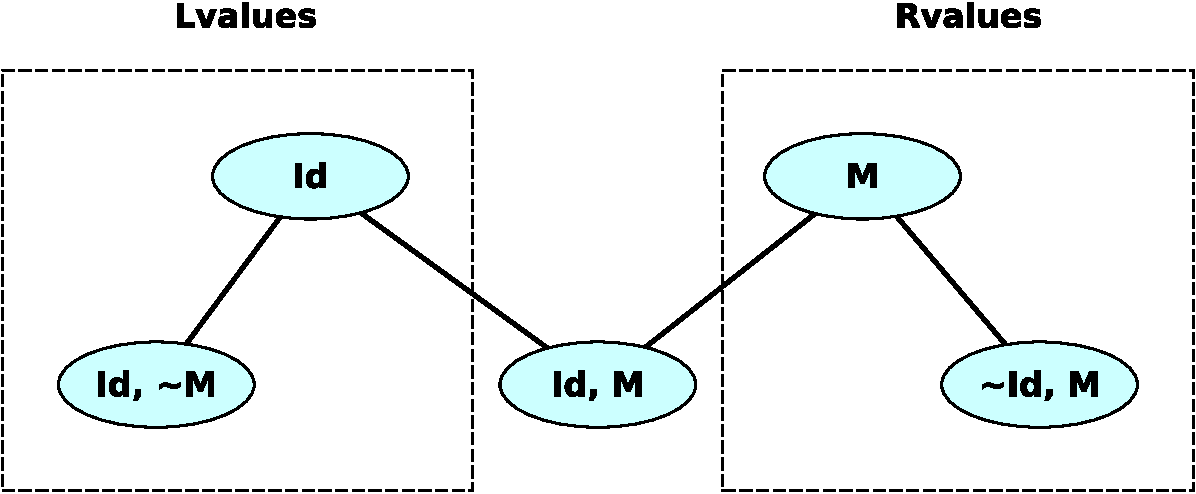
\includegraphics[width=0.8\textwidth]{illustrations/rvref-identity-crop.pdf}
\caption{Идентичность и перемещаемость}
\label{fig:rvref-identity}
\end{figure}

Здесь объекты, обладающие идентичностью называются glvalues (или generalized lvalues), а обладающие  перемещаемостью это rvalues. Перемещаемость без идентичности это prvalues, а идентичность без перемещаемости это lvalues. И, наконец, самые странные штуки в середине, обладающие и тем и другим это xvalues.

xvalue (от expiring value) это значение, возвращённое из функции по правой ссылке, например \lstinline!move(x)! это xvalue.

Стандарт предлагает функторы-определители.

\begin{itemize}
\item \lstinline!is_rvalue_reference<T>::value! определяет является ли  тип xvalue
\item \lstinline!is_lvalue_reference<T>::value! определяет является ли тип lvalue
\end{itemize}

Например

\begin{lstlisting}
int x = 42;
assert(is_lvalue_reference<decltype(x)>::value);
assert(is_rvalue_reference<decltype(move(x))>::value);
\end{lstlisting}

Имея только два эти функтора, остальные категории значений можно лего определить используя их комбинации.

\begin{verbatim}
prvalue = ~xvalue & ~lvalue
glvalue = xvalue & lvalue
rvalue = xvalue & ~lvalue
\end{verbatim}

Пожалуй есть всего три функции, для которых имеет смысл возвращать правую ссылку (то есть производить xvalue result)

\begin{itemize}
\item \lstinline!std::move!
\item \lstinline!std::forward!
\item \lstinline!std::declval!
\end{itemize}

Если вы хотите написать свою функцию, которая будет возвращать \lstinline!&&!, это значит, что вы что-то делаете не так, или вы хотите ещё раз написать одну из упомянутых выше функций.

\ifgalvanic
\pagebreak
\section{Гальваническая развязка}\label{PImpl}

TODO: после расформирования главы про исключения, идиома PImpl осталась неприкаянной. Тут будет что-то про неё, может быть с какими-нибудь примерами

Кроме того PImpl отлично мотивирует наследование
\fi

\pagebreak
\section{Наследование интерфейса\index{Inheritance}\index{Interface inheritance}}\label{IntfInheritance}

\hfill\textit{If you think C++ is not overly complicated, just what is} 

\hfill\textit{a protected abstract virtual base pure virtual private destructor?}

\hfill\textit{And when was the last time you needed one?}{\vspace{0.5em}}

\hfill\textit{-- Tom Cargill}

Программа, в которой важной абстракцией является физический объект, иногда подразумевает сложные архитектурные решения, относительно представления этого объекта. Координаты нужны (почти) всем физическим объектам, но как быть с массой, с радиусом, с электрическим зарядом, с любыми дополнительными параметрами? Конечно можно написать один тип со всем богатством возможностей внутри него

\begin{lstlisting}
class AnyPhysicalBody
{
private:
  double x, y, z;
  double vx, vy, vz;
  double m;
  double r;
/* ... */
public:
  int move (double dt);
};
\end{lstlisting}

Но создавать объект такого типа, когда нужна всего лишь материальная точка с массой -- означает тащить за собой массу ненужных полей с произвольными и не нужными значениями. Это называется overhead -- пустая трата памяти и машинного времени. Вторая возможность -- написать небольшие конкретные типы на каждый случай:

\begin{lstlisting}
class CelestialBody
{
  double x, y;
  double vx, vy
  double m;
public:
/* ... */
  int move (double dt);
  int apply_force (double f, double dt);
};

class Planet
{
  double x, y;
  double vx, vy
  double m;
  double r;
public:
/* ... */
  int move (double dt);
  int apply_force (double f, double dt);
  int detect_collision (const Planet *rhs) const;
  int detect_collision (const CelestialBody *rhs) const;
};
\end{lstlisting}

Это работает, но возникают две проблемы: методы \lstinline!detect_collision! внутри класса \lstinline!Planet! дублируются (это не страшно, но может быть неприятно) и гораздо более печальная проблема -- принципиально разные типы \lstinline!Planet! и \lstinline!CelestialBody! теперь не могут быть объединены, скажем в массив указателей на небесные тела. Решение этой проблемы состоит в том, чтобы указать компилятору на \textbf{общий интерфейс} или на то, что планета тоже является небесным телом (и материальной точкой).

\subsection{Чисто виртуальные функции и абстрактные классы}\label{PureVirtual}

Интерфейсным или чисто абстрактным является пользовательский тип, в котором определён хотя бы один \textbf{чисто виртуальный} метод. Ключевое слово \lstinline!virtual! предусматривает довольно сложное поведение и будет подробно рассмотрено в (\ref{VirtualUnderHood}). Чисто виртуальные методы легко различать по спецификации \lstinline!=0!. Хорошим тоном является писать тип, полностью состоящий из таких методов.

\begin{lstlisting}
struct ICelestialBody
{
  virtual double get_x () const = 0;
  virtual double get_y () const = 0;
  virtual int move (double dt) = 0;
  virtual int apply_force (double f, double dt) = 0;
};
\end{lstlisting}

Объекты такого типа нельзя создавать, его методы не могут иметь реализации, поэтому такой класс называется \textbf{абстрактным}. Это общий интерфейс -- обещание того, что все реализующие его пользовательские типы реализуют две именно такие функции. Такое обещание пользовательский тип может дать через механизм открытого наследования интерфейса.

\begin{lstlisting}
class CelestialBody: public ICelestialBody
{
  double x, y;
  double vx, vy;
  double m;
public:
/* ... */
/* ICelestialBody implementation */
  double get_x () const { return x; }
  double get_y () const { return y; }
  int move (double dt); 
  int apply_force (double f, double dt);
/* ... */
};
\end{lstlisting}

Синтаксис открытого наследования очевиден из примера. Указание модификатора \lstinline!public! обязательно, поскольку наследование может быть и иным см. (\ref{OtherInheritance}). Для выражения идиомы ``реализация интерфейса'' подходит только открытое наследование. 

\begin{lstlisting}
class Planet: public ICelestialBody
{
  double x, y;
  double vx, vy;
  double m;
  double r;
public:
/* ... */
/* ICelestialBody implementation */
  double get_x () const { return x; }
  double get_y () const { return y; }
  int move (double dt);
  int apply_force (double f, double dt);
  int detect_collision (const ICelestialBody &rhs) const;
};
\end{lstlisting}

Разумеется, каждый класс может открыто наследовать от любого количества интерфейсов, но на данном этапе имеет смысл ограничиться одиночным наследованием, отложив рассмотрение обобщений до (\ref{MultipleInheritance}).

Визуально открытое наследование интерфейса представляет UML-диаграммой, показанной на (рис. \ref{fig:inheritance-interface}).

\begin{figure}[ht]
\centering
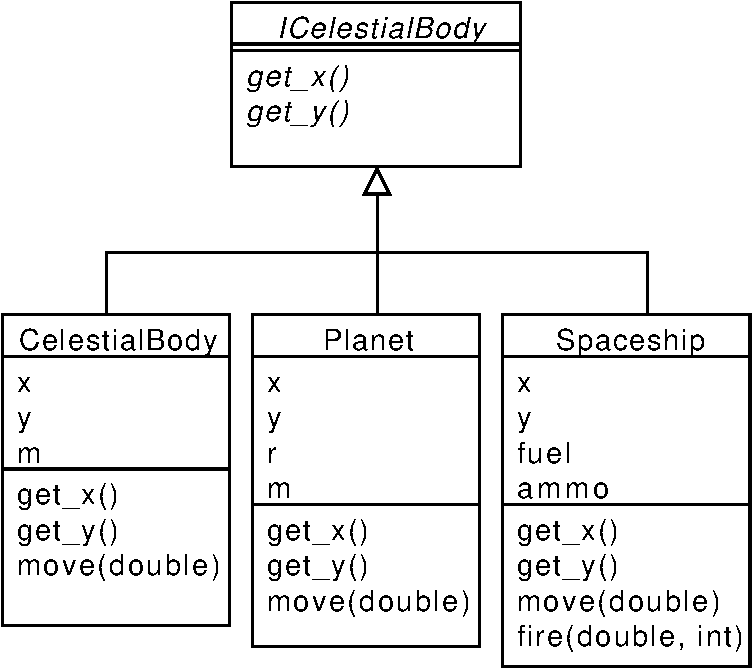
\includegraphics[width=0.8\textwidth]{illustrations/intf-inheritance-crop.pdf}
\caption{Открытое наследование интерфейса}
\label{fig:inheritance-interface}
\end{figure}

Теперь можно писать довольно абстрактный код, использующий приведение указателя или ссылки на объект, к указателю или ссылке на его открытый интерфейс. Как обычно сначала полезно написать небольшую служебную функцию:

\begin{lstlisting}
int 
in_between (double x, double ymin, double ymax)
{
  return (x <= ymax) && (x >= ymin);
}
\end{lstlisting}

И определить

\begin{lstlisting}
int 
Planet::detect_collision (const ICelestialBody &rhs) const
{
  return in_between (rhs.get_x(), x - r, x + r) && 
         in_between (rhs.get_y(), y - r, y + r);
}
\end{lstlisting}

Совершенно неважно с чем может произойти столкновение, если это ``что-то'' поддерживает все методы \lstinline!ICelestialBody!:

\begin{lstlisting}
Planet Jupiter;
Planet Earth;
CelestialBody Gallea;
/* .. */

Earth.detect_collision(Jupiter); 
Earth.detect_collision(Gallea);
\end{lstlisting}

Это похоже на общий разъём розетки, куда в стандартный интерфейс можно подключить много разных уcтройств (рис. \ref{fig:common-intf}).

\begin{figure}[ht]
\centering
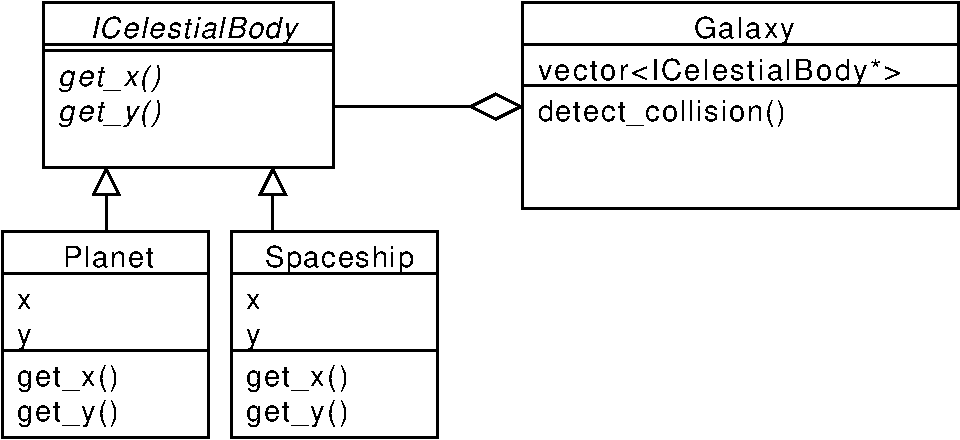
\includegraphics[width=1.0\textwidth]{illustrations/common-intf-crop.pdf}
\caption{Открытый интерфейс как общий разъём для подключения}
\label{fig:common-intf}
\end{figure}

Аргумент \lstinline!rhs! передан по константной ссылке. В принципе, он мог бы быть передан и по обычной ссылке и по (константному) указателю:

\begin{lstlisting}
int 
Planet::detect_collision (const ICelestialBody *rhs)
{
  return in_between (rhs->get_x(), x - r, x + r) && 
         in_between (rhs->get_y(), y - r, y + r);
}
\end{lstlisting}

По понятным причинам в случае абстрактного базового класса, аргумент не может быть передан по значению, так как не может быть сконструирован объект такого типа.

\subsection{Статический и динамический тип\index{Dynamic type}}\label{StatDynPoly}

Функция \lstinline!Planet::detect_collision! вызывает внутри себя виртуальную функцию \lstinline!ICelestialBody::get_x()! которая имеет один неявный аргумент -- указатель \lstinline!this! того объекта, для которого она вызвана. Этот указатель протягивается через формальный аргумент. 

Что можно сказать об аргументе \lstinline!rhs!? Всего лишь, что его тип, объявленный в списке аргументов (иначе говоря статический тип) это константная ссылка на \lstinline!ICelestialBody!. Это всё, что компилятор может сказать об этом типе \textbf{статически}, без контекста исполнения.

Но \textbf{динамически}, при вызове из \lstinline!main!, функция \lstinline!detect_collision! вызывается из двух разных мест с двумя разными параметрами, один из которых имеет тип \lstinline!Planet!, другой – тип \lstinline!CelestialBody! и именно эти типы имеет указатель \lstinline!this! для которого вызывается \lstinline!get_x()! в первом и во втором случае.

При вызове функции, она должна быть верно связана с именем типа, поскольку имя типа участвует в манглированном имени функции, как это объяснялось в (\ref{NameResolution}). При обычном вызове функции или метода, она связывается со своим типом статическим или ранним связыванием. Динамическое или позднее связывание работает при вызове виртуальной функции по ссылке или указателю на интерфейс. При этом решение о том какая функция в действительности будет вызвана, откладывается до момента вызова и принимается на основании её динамического типа. Обычно это требует дополнительного уровня косвенности для вызова через таблицу виртуальных методов, которая будет рассмотрена в (\ref{VirtualUnderHood}).

Если при динамическом связывании, функция имеет аргумент, который может принимать значения разных динамических типов с которыми она вызвана, этот аргумент называется \textbf{полиморфным} аргументом для динамического полиморфизма, а сама функция -- полиморфной (динамически полиморфной) функцией. В случае любой виртуальной функции единственный её полиморфный аргумент -- неявный указатель на объект, для которого она вызвана.

Вообще говоря, динамический тип может быть разрешён в любой базовый класс, в том числе и в абстрактный. При этом производится попытка прямого вызова чисто виртуальной функции. Это ошибка, но язык C++ всегда даёт программисту возможность выстрелить себе в ногу, это фирменный стиль. Поэтому важно знать тот случай, когда это наиболее часто может произойти.

\subsection{Подробнее о чисто виртуальных функциях}\label{VirtualUnderHood}

Чтобы понять, что именно делает компилятор для того, чтобы вызов по указателю на интерфейс делегировался верному динамическому типу, полезно попробовать написать нечто подобное на C.

Сначала определяется таблица виртуальных методов

\begin{lstlisting}
typedef double (get_t)(void *);

struct celestial_body_vmt
{
  get_t *pget_x;
  get_t *pget_y;
/* ... */
};
\end{lstlisting}

Дальше указатель на эту таблицу идёт в структуру интерфейса:

\begin{lstlisting}
struct icelestial_body
{
  struct celestial_body_vmt vtable;
  /* ... */
};
\end{lstlisting}

Инициализация VMT происходит в конструкторе интерфейса:

\begin{lstlisting}
void
icelestial_ctor(struct icelestial_body *ths, get_t *pget_x, get_t *pget_y)
{
  ths->vtable.pget_x = pget_x;
  ths->vtable.pget_y = pget_y;
  /* ... */
}
\end{lstlisting}

Каждый класс-наследник содержит в себе интерфейсную часть и собственную реализацию интерфейсных функций:

\begin{lstlisting}
struct celestial_body
{
  struct icelestial_body intf;
  double x, y;
  /* ... */
};

double celestial_get_x(void *ths) { return ((struct celestial_body *)ths)->x; }
double celestial_get_y(void *ths) { return ((struct celestial_body *)ths)->y; }
\end{lstlisting}

Конструктор класса-наследника устанавливает известные ему функции в таблицу виртуальных функций интерфейсного класса:

\begin{lstlisting}
void 
celestial_ctor(struct celestial_body *ths)
{
  icelestial_ctor (&ths->intf, &celestial_get_x, &celestial_get_y);
  /* ... */  
}
\end{lstlisting}

Теперь всё готово для того, чтобы правильно сконструированный объект наследника мог участвовать в обобщённом коде наподобие уже рассмотренного collision detection (для простоты можно не рассматривать детали планет, имеющих некий радиус, а принять столкновение двух небесных тел как прохождение их на расстоянии epsilon):

\begin{lstlisting}
int
detect_collision (struct icelestial_body *lhs, struct icelestial_body *rhs)
{
  double x = lhs->vtable.pget_x(lhs);
  double y = lhs->vtable.pget_y(lhs);
 
  return in_between (rhs->vtable.pget_x(rhs), x - epsilon, x + epsilon) && 
         in_between (rhs->vtable.pget_y(rhs), y - epsilon, y + epsilon);
}
\end{lstlisting}

Вызов этого кода требует конструирования (вручную, поскольку используется C). Крайне многословный код, но так бывает всегда в недосахаренных системах.

\begin{lstlisting}
struct celestial_body Gallea;
struct celestial_body Encke;

celestial_ctor (&Gallea);
celestial_ctor (&Encke);

/* ... */

detect_collision (&Gallea.intf, &Encke.intf);
\end{lstlisting}

Таким образом, очевидно насколько много компилятор C++ прячет под капот. Знание механики работы виртуальных функций необязательно, но часто и очень сильно помогает. Например теперь ясно, что если бы передача параметров внутрь \lstinline!detect_collision! шла по значению, то они должны были быть сконструированы внутри функции. Но поскольку у \lstinline!icelestial_body! нет собственных координат и нет методов, чтобы их вернуть, то единственное, что можно передать в такой конструктор это нули:

\begin{lstlisting}
int
detect_collision (struct icelestial_body lhs, struct icelestial_body rhs)
{
  double x, y;
  
  icelestial_ctor (&lhs, 0, 0);
  icelestial_ctor (&rhs, 0, 0);

  x = lhs->vtable->pget_x();
  y = lhs->vtable->pget_y();
 
  return in_between (rhs->vtable->pget_x(), x - epsilon, x + epsilon) && 
         in_between (rhs->vtable->pget_y(), y - epsilon, y + epsilon);
}
\end{lstlisting}

И тогда вызов чисто виртуальной функции превращается в аналог вызова функции по нулевому указателю. При передаче же по указателю происходит всего лишь его приведение к указателю другого типа, без потери данных. Подобным образом работает и передача по ссылке в C++. Есть ещё несколько поучительных уроков: наличие дополнительного расхода памяти в каждом объекте на таблицу виртуальных функций, наличие дополнительной косвенности по вызову, ухудшение возможностей компилятора для инлайн-подстановки довольно простых методов и так далее -- всё это очевидно при понимании того, как вещи функционируют на самом деле.

Теперь самое время разобрать несколько хитрых вопросов, относящихся к наследованию интерфейса:

\subsection{Параметры по умолчанию\index{default arguments}}\label{DefArguments}

Тонкий вопрос, который многие программисты на C++ часто упускают из виду это то, как ведут себя виртуальные функции с параметрами по умолчанию. Если параметр по умолчанию в интерфейсе изменён в одном из его наследников:

\begin{lstlisting}
struct ICelestialBody
{
/* ... */
  virtual int apply_force (double f, double dt = 0.1) = 0;
};

void 
forcesApply (ICelestialBody *pbody, double *pfs, int n)
{
  for (; n > 0; --n)
    pbody->apply_force(pfs[n - 1]);
}

class CelestialBody: public ICelestialBody
{
public:
/* ... */
  int apply_force (double f, double dt = 0.01);
};
\end{lstlisting}

После чего этот обобщённый код вызван для конкретного динамического типа:

\begin{lstlisting}
double fs[5] = {1.0, 1.5, 1.2, 1.8, 1.10};
CelestialBody t;
forcesApply (&t, fs, 5);
\end{lstlisting}

Казалось бы -- реально будет вызвана функция \lstinline!apply_force! из класса \lstinline!CelestialBody! и логично ожидать значение аргумента по умолчанию таким, как он выставлен там. Но в реальности эта функция будет вызвана со значением аргумента по умолчанию, выставленным в интерфейсе.

Дело в том, что функции в C++ связываются динамически, а аргументы по умолчанию – статически. Если вернуться к сишному аналогу, можно легко увидеть, что в таблице виртуальных функций нет места для хранения и перезаписи аргументов по умолчанию.

\subsection{Виртуальные деструкторы}\label{VirtDestr}

Для программиста на C++ важно знать один очень специальный случай полиморфизма, относящийся к семантике освобождения, а именно виртуальные деструкторы. Рассмотрим пример – пусть у нас есть фабричная функция, которая в зависимости от радиуса желаемого пользователем небесного тела возвращает \lstinline!CelestialBody! если он меньше порогового значения или планету в другом случае:

\begin{lstlisting}
ICelestialBody *get_celestial_body (double r) {
  if (r < epsilon)
    return new CelestialBody ();

  return new Planet ();
}
\end{lstlisting}

Что произойдёт если планета была получена через эту функцию, а потом удалена из памяти обычным способом?

\begin{lstlisting}
ICelestialBody *planet = get_celestial_body (100.0);
/* ... */
delete planet;
\end{lstlisting}

Будет освобождена базовая часть, но не будет освобождена производная часть, что неминуемо приведёт к утечкам памяти и проблемам. 

Решение этой проблемы: сделать деструктор виртуальным в интерфейсе. Тогда будет автоматически правильно вызван деструктор производного класса по указателю на базовый.

\begin{lstlisting}
struct ICelestialBody
{
  virtual double get_x () const = 0;
  virtual double get_y () const = 0;
  virtual int move (double dt) = 0;
  virtual int apply_force (double f, double dt) = 0;
  virtual ~ICelestialBody() {}
};
\end{lstlisting}

Наличие в классе невиртуального деструктора является в мире промышленного программирования достаточным основанием никогда ничего не наследовать от этого класса. Обратное – дурной тон. 

\subsection{Тела для чисто виртуальных функций}\label{VirtdestrBody}

\textbf{Вопрос к студентам:} можно ли объявить деструктор чисто виртуальным следующим образом:

\begin{lstlisting}
struct ICelestialBody
{
  /* ..... */
  virtual ~ICelestialBody() = 0;
};
\end{lstlisting}

\ifanswers
Правильный ответ: да, можно, но это приведет к pure virtual function call при попытке унчитожить любого наследника такого класса.
\fi

Тем не менее, иногда чисто виртуальный деструктор имеет смысл -- например если это единственная функция в интерфейсе. Выход: написать тело для чисто виртуального деструктора

\begin{lstlisting}
virtual ICelestialBody::~ICelestialBody()
{
}
\end{lstlisting}

В том случае, если у чисто виртуальной функции существует тело, эта функция всё ещё не может быть вызвана как метод своего класса, но она может быть вызвана из любого своего наследника.

\textbf{Вопрос к студентам:} как вы думаете зачем ещё может быть использована эта техника?

\ifanswers
Возможный ответ: для организации разумного поведения по умолчанию, которое наследники должны явно вызывать:

\begin{lstlisting}
class B 
{
public:
  virtual bool f() = 0;
};

bool 
B::f() 
{
  return true;  // this is a good default, but
}               // shouldn't be used blindly

class D : public B 
{
public:
  bool f() 
  {
    return B::f(); // if D wants the default
  }                // behaviour, it has to say so
};
\end{lstlisting}

Но тут возможны и другие варианты: например выдать лучшее сообщение об ошибке чем компилятор и выйти.
\fi

\subsection{Виртуальные конструкторы}\label{VirtCtors}

Статическая функция не может в общем случае быть ни виртуальной ни (тем более) чисто виртуальной. Поэтому конструкторы тоже не могут быть виртуальными.

\textbf{Вопрос к студентам:} а нужны ли нам вообще виртуальные конструкторы?

\ifanswers
Правильный ответ: да очень нужны. Скажем виртуальный конструктор копирования позволил бы создать в явном виде объект производного класса по указателю на объект базового класса
\fi

На этом нужно остановиться особо. Было упомянуто (см. \ref{RAII}), что для RAII фундаментальные переопределяемые функции это конструктор копирования и оператор присваивания. И вдруг оказывается, что второй может быть виртуальным, а первый никак:

\begin{lstlisting}
class IVector
{
public:
  virtual IVector& operator= (const IVector &rhs) = 0; // OK
  virtual IVector(const IVector *rhs) = 0; // ERROR
};
\end{lstlisting}

Приходится выкручиваться. Обычно в рамках выкручивания люди заводят виртуальную функцию \lstinline!clone! для получения копии объекта производного класса по указателю на базовый класс:

\begin{lstlisting}
class IVector
{
public:
  virtual IVector* clone() = 0; // virtual ctor idiom
  virtual void operator+= (const IVector &lhs) = 0;
};

class Vector : public IVector
{
public: 
  Vector (const Vector &rhs); // copy ctor
  void operator+= (const IVector &lhs); // add any vector to given
  IVector *clone() {
    return new Vector(*this);
  }
};

class SparceVector : public IVector
{
public: 
  SparceVector (const SparceVector &rhs); // copy ctor
  void operator+= (const IVector &lhs); // add any vector to given
  IVector *clone() {
    return new SparceVector(*this);
  }
};
\end{lstlisting}

Теперь общий код для сложения, которое поддерживает как обычные так и разреженные вектора можно реализовать в терминах виртуальных конструкторов:

\begin{lstlisting}
IVector *add (const IVector &rhs, const IVector &lhs)
{
  IVector &result = *rhs.clone();
  result += lhs;
  return &result;
}
\end{lstlisting}

Эта идиома крайне полезна и возмещает очевидный недостаток языка C++ в части виртуального конструирования.

\textbf{Вопрос к студентам:} но почему такой недостаток вообще есть? Что мешает сделать в языке настоящие виртуальные конструкторы?

\ifanswers
Правильный ответ: именно конструктор делает ту работу, которая должна быть сделана чтобы заработал механизм виртуальных функций. Поэтому в конструкторе класса виртуальные вызовы работают как не виртуальные. Поэтому даже если бы можно было сделать конструктор виртуальным, его вызов все равно был бы вызовом невиртуальной функции.
\fi

\pagebreak
\section{Наследование реализации}\label{ImplInheritance}

\hfill\textit{Inheritance is the base class of Evil} {\vspace{0.5em}}

\hfill\textit{-- Sean Parent}

Разработанные в (\ref{PureVirtual}) классы-наследники \lstinline!CelestialBody! и \lstinline!Planet! всё ещё имеют слишком много дублирующегося кода: общие поля координат и скоростей, общие и притом идентичные селекторы координат. Это обычная и, более того, достаточно частая ситуация. Для уменьшения дублирования в классе \lstinline!Planet!, можно заметить, что планета также \textbf{является} небесным телом, отличаясь только тем, что у неё имеет значение радиус и есть дополнительный метод для определения столкновений. Это отношение ``быть частным случаем'' также, как и отношение ``реализовать интерфейс'' моделируется открытым наследованием, но в данном случае унаследована будет и реализация некоторых методов и поля класса \lstinline!CelestialBody!, такие как \lstinline!x! и \lstinline!y!. Общий интерфейс тот же:

\begin{lstlisting}
struct ICelestialBody
{
  virtual double get_x () const = 0;
  virtual double get_y () const = 0;
  virtual int move (double dt) = 0;
  virtual int apply_force (double f, double dt) = 0;
  virtual ~ICelestialBody() {}
};
\end{lstlisting}

Пользовательский тип \lstinline!CelestialBody! всё так же реализует общий интерфейс:

\begin{lstlisting}
class CelestialBody: public ICelestialBody
{
protected:
  double x, y;
  double vx, vy;
  double m;
public:
/* ... */
/* ICelestialBody implementation */
  double get_x () const { return x; }
  double get_y () const { return y; }
  int move (double dt); 
  int apply_force (double f, double dt);
/* ... */
};
\end{lstlisting}

Новое ключевое слово \lstinline!protected! сообщает, что все помеченные им поля при открытом наследовании будут доступны производным классам.

Пользовательский тип \lstinline!Planet! сообщает, что является уточнением \lstinline!CelestialBody!:

\begin{lstlisting}
class Planet: public CelestialBody
{
  double r;
public:
  int detect_collision (const ICelestialBody &rhs) const;
};
\end{lstlisting}

Теперь есть необходимость определить расстояние между небесными телами. Соответствующий обобщённый код:

\begin{lstlisting}
double 
get_distance (const ICelestialBody &lhs, 
              const ICelestialBody &rhs)
{
  double xdist = lhs.get_x() - rhs.get_x();
  double ydist = lhs.get_y() - rhs.get_y();

  return sqrt (xdist*xdist + ydist*ydist);
}
\end{lstlisting}

Вполне может быть вызван так:

\begin{lstlisting}
Planet Jupiter;
Planet Earth;

/* ... */

double d = get_distance (Jupiter, Earth);
\end{lstlisting}

Несмотря на то, что функций \lstinline!Planet::get_x! и \lstinline!Planet::get_y! попросту не существует, у класса \lstinline!Planet! тем не менее есть эти методы, унаследованные от класса \lstinline!CelestialBody!. Внутри функции \lstinline!Planet::get_distance!, динамический тип \lstinline!Planet! аргумента \lstinline!lhs! позволяет сделать вызов общей для \lstinline!Planet! и \lstinline!CelestialBody! функции, которая изменяет их общую открытую часть.

TODO: где-то здесь про vtable not found problem (случай интерфейса с недоопределёнными функциями).

Существенное отличие открытого наследования от наследования интерфейса -- класс не только даёт обещание, что будет поддерживать тот или иной интерфейс, но ещё и заимствует у базового класса конкретную реализацию, оставляя себе только уточнение специфичных для себя методов. Эта техника существенно улучшает переиспользование кода и может быть в произвольной пропорции смешана с чисто абстрактными классами: например вполне можно было бы внести координаты и их селекторы в интерфейсный класс, у которого в этом случае появилась бы часть интерфейса который наследники должны реализовать (чисто виртуальные функции) и часть реализации, которая просто наследуется для использования. Впрочем смешивать такие вещи -- не всегда полезно.

Теперь UML-диаграмма становится более иерархичной, как показано на (рис. \ref{fig:inheritance-implementation}).

\begin{figure}[h!]
\centering
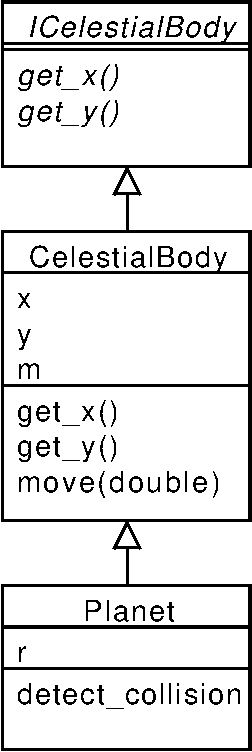
\includegraphics[width=0.3\textwidth]{illustrations/impl-inheritance-crop.pdf}
\caption{Открытое наследование реализации}
\label{fig:inheritance-implementation}
\end{figure}

Можно заметить, что сверху вниз по этой диаграмме, более общие понятия предшествуют более частным. Скажем ``конкретное небесное тело'' это ``небесное тело вообще'', а планета это и то и другое. При открытом наследовании все открытые члены базового класса доступны как открытые члены производного класса, а также работает неявное преобразование типа от производного к базовому классу. Говорят, что открытое наследование \textbf{моделирует} отношение ``is-a'', при котором объект производного класса является объектом базового класса (в том смысле, в каком планета является небесным телом). Это отношение довольно важно, подробнее см. (\ref{LSP}).

Увы, с точки зрения ООП на C++ такая диаграмма имеет фундаментальный и очевидный недостаток: конкретный класс \lstinline!CelestialBody! является базовым при наследовании. Это может привести к одной неприятной проблеме.

\subsection{Проблема срезки\index{Cutting}}\label{Cutting}

Можно ещё раз рассмотреть функцию \lstinline!detect_collision!, на этот раз остановившись на её параметрах. В диаграмме (рис. \ref{fig:inheritance-implementation}) не очевидно, что там должен стоять указатель на \lstinline!ICelestialBody!. Кажется достаточно простого указателя на \lstinline!CelestialBody! -- в конце концов это по факту общий интерфейс для всех объектов у которых можно запросить координаты.

Увы, это делает возможным передачу аргументов по значению.

\begin{lstlisting}
Planet::detect_collision (CelestialBody rhs) /* Oops */
\end{lstlisting}

Проблема понятна: формальные аргументы, переданные по значению конструируются при входе в функцию. Попытка сконструировать объект абстрактного класса (то есть класса, содержащего хотя бы один чисто виртуальный метод) сама по себе ошибочна. Но здесь компилятор уже не защищает от такого ошибочного конструирования. В этом случае новосконструированный объект \lstinline!rhs! будет иметь динамический тип \lstinline!CelestialBody! независимо от динамического типа аргументов. 

\begin{lstlisting}
Planet jupiter, earth;
jupiter.detect_collision(earth); // sliced
\end{lstlisting}

Здесь переданная планета была срезана до обычного небесного тела, то есть потеряла как минимум поле с радиусом. Для более сложных классов, их состояние вообще может потерять тот или иной инвариант.

В лучшем случае срезки вызов функции \lstinline!get_x()! будет связан с чисто виртуальной заглушкой интерфейса и программа будет прервана по ошибке. 

Этот срез информации при передаче по значению называется ``проблемой срезки'' (object slicing). Срезка часто возникает в практических контекстах и важно о ней помнить.

\subsection{Идиома NVI и разделение обязанностей}\index{NVI}\label{NVI}

Одним из способов бороться с проблемой срезки и одновременно сохранить наследование реализации может быть вынесение большинства функциональности и даже полей в абстрактный базовый класс, как показано на (рис. \ref{fig:better-implinhh})

\begin{figure}[h!]
\centering
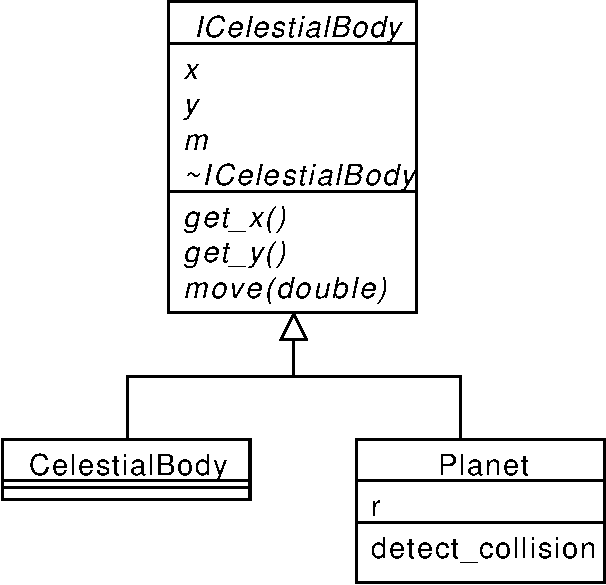
\includegraphics[width=0.7\textwidth]{illustrations/better-implinh-crop.pdf}
\caption{Способ делать конкретными классами только листья}
\label{fig:better-implinhh}
\end{figure}

\textbf{Домашняя наработка:} напишите код к этой UML-диаграмме

Делать конкретными классами только листья -- совет который разделяют многие авторы, для примера можно указать Майерса \cite{effcpp3d}.

Но такой подход порождает проблемы: функция \lstinline!get_x! больше не требует переопределения в наследниках (все ещё допуская его) и поэтому кто-то может забыть её переопределить, получив при этом странное поведение по умолчанию. Здесь уместен известный анекдот про кенгуру в программе-тренажере для летчиков (класс кенгуру был для простоты и от нехватки времени унаследован от класса пехотинец с соответствующими последствиями во время работы программы -- пилоты были поражены тактической слаженностью кенгуру а так же попытками стаи кенгуру запустить по самолету ``стингер'').

Выходом является разделить обязанности предоставления поведения по умолчанию и заглушки для переопределения:

\begin{lstlisting}
struct ICelestialBody {
public:
  /* Non-Virtual interface */
  double get_x () const { return do_get_x(); }
  double get_y () const { return do_get_y(); }
  virtual ~ICelestialBody() = 0 {}

protected:
  double m_x, m_y;

private:
  virtual double do_get_x () = 0 { return m_x; }
  virtual double do_get_y () = 0 { return m_y; }
};
\end{lstlisting}

\textbf{Домашняя наработка:} нарисуйте UML-диаграмму с планетами и небесными телами к этому коду.

Эта идиома называется NVI (non-virtual interface) и крайне полезна. Один из таких полезных случаев будет рассмотрен далее, в (\ref{NameHiding}).

Кроме того, эта идиома окажется на удивление полезной при рассмотрении полиморфных аллокаторов в (\ref{sub:polyalloc}), когда разговор зайдёт за стандартную библиотеку.

\subsection{Тонкости скрытия имён}\label{NameHiding}

При наследовании реализации имена имеют значение. Если некий класс \lstinline!Matrix! определяет две версии \lstinline!pow! (для возведения в целую степень, что гораздо проще и в вещественную, что сложнее):

\begin{lstlisting}
class Matrix {
public:
  virtual void pow(int x);
  virtual void pow(double x);
};
\end{lstlisting}

То какой-то его наследник может решить переопределить только одну из них:

\begin{lstlisting}
class SparceMatrix : public Matrix
{
public:
  void pow (int x);
};
\end{lstlisting}

Увы, это плохая идея. При следующем вызове:

\begin{lstlisting}
SparceMatrix t;
/* ..... */
t.pow(5.0);
\end{lstlisting}

Произойдёт вовсе не вызов \lstinline!Matrix::pow(double)! а вместо этого неявное преобразование типа и вызов \lstinline!SparceMatrix::pow(int)!. Чтобы избежать такого поведения можно явно ввести имя базового класса в контекст производного класса:

\begin{lstlisting}
class SparceMatrix : public Matrix {
public:
  using Matrix::pow;
  void pow (int x);
};
\end{lstlisting}

Либо можно воспользоваться идиомой NVI и переопределять закрытые функции с разными именами:

\begin{lstlisting}
class Matrix {
public:
  /* Non-virtual interface */
  void pow(int x) { do_pow_int(x); }
  void pow(double x) { do_pow_dbl(x); }
private:
  virtual void do_pow_int(int x);
  virtual void do_pow_dbl(double x);
};
\end{lstlisting}

Здесь снова разделяется поведение по умолчанию и заглушки для переопределения.

\subsection{Закрытое и защищенное наследование}\label{OtherInheritance}

\hfill\textit{The object-oriented version of 'Spaghetti code' is,}

\hfill\textit{of course, 'Lasagna code'}{\vspace{0.5em}}

\hfill\textit{-- Roberto Waltman}

Существенно иначе обстоят дела с закрытым наследованием. При закрытом наследовании, неявного преобразования типа от производного к базовому не задаётся, а все открытые методы базового класса становятся закрытыми методами производного класса, как показано в таблице ниже:

\begin{center}
  \begin{tabular}{ | l | c | c | r | }
    \hline
    modifier & public & protected & private \\ \hline \hline
    public & public & protected & private \\ \hline
    protected & protected & protected & private \\ \hline
    private & private & private & private \\ \hline
  \end{tabular}
\end{center}

Важно понимать, что в эту таблицу сведена внешняя видимость полей и методов класса. Внутрення видимость и видимость для наследников остаётся прежней.

Говорят, что закрытое наследование моделирует отношение part-of (быть частью). В принципе у закрытого наследования нет почти никакой разницы с композицией:

\begin{lstlisting}
struct Engine {
  int start() const;
};
\end{lstlisting}

Теперь этот двигатель может быть включен в космический корабль посредством композиции

\begin{lstlisting}
class SpaceShip_p {
  Engine e;
public:
  int start (double dt) const { e.start(); } 
};
\end{lstlisting}

Или же посредством закрытого наследования.

\begin{lstlisting}
struct SpaceShip_p : private Engine {
  int start (double dt) const { Engine::start(); }
};
\end{lstlisting}

Впрочем одна тонкая разница будет видна при разговоре о множественном наследовании.

Защищенное наследование не слишком популярно в C++, однако автору удалось найти одно интересное применение (вынесено в тест по этой части курса).

\subsection{Конструкторы базовых классов}\label{BaseClassConstr}

При конструировании каждого класса будут неявно вызваны конструкторы его базовых классов по умолчанию, если они не вызваны явно в списке инициализации. Если эти конструкторы нетривиальные, то они, соответственно \textbf{должны} быть явно вызваны в списке инициализации:

\begin{lstlisting}
class A
{
  int x_;
public:
  A(int x) : x_(x) {}
};

class B : public A
{
public:
  B() {} // error!
  B(int x) : A(x) {} // ok
};
\end{lstlisting}

Здесь ошибка при попытке дефолтной инициализации вызвана тем, что подобъект класса \lstinline!A! должен быть инициализирован, но нет.

Необходимо понимать, что время жизни объекта начинается после того, как отработал его конструктор. Это означает, что следующий код (хотя и корректен с точки зрения языка) не верен:

\begin{lstlisting}
class A {
  public:
    A (const char *s) {}
    const char *f() { return "hello, world"; }
};

class B : public A {
  public:
    B() : A ( s = f() ) {}
  private:
    const char *s;
};
\end{lstlisting}

Здесь сразу две ошибки. Во-первых попытка вызвать метод \lstinline!f()! базового подобъекта, который ещё не сконструирован в этой точке (поскольку только вызывается его конструктор). Это может прокатить, может нет, но это в любом случае некорректно. Во-вторых попытка инициализировать и потом использовать ещё не существующий член производного класса (до конструирования которого там пока вообще далеко).

Не следует допускать таких ошибок в своём коде.

\subsection{Больше возможностей для полиморфизма}\label{NewVirtual}

Начиная с C++11 в язык было введено несколько дополнительных возможностей, которых часто действительно не хватало и которые будут рассмотрены ниже.

В разделе (\ref{NameHiding}) уже рассматривалась возможность неявных ошибок из-за разрешения имен в стиле C++. Теперь настало время рассмотреть ещё одну ошибку такого рода и что с этим делать. Итак, всё те же матрицы.

\begin{lstlisting}
struct Matrix {
  virtual void pow(int x);
};
\end{lstlisting}

И тут программист совершает обычную человеческую ошибку.

\begin{lstlisting}
struct SparceMatrix : Matrix {
  void pow (long x); // oops
};
\end{lstlisting}

Увы, эта функцию вовсе не перегружает исходную функцию \lstinline!pow! и в каком-нибудь сложном динамическом контексте могут быть неприятные сюрпризы. 

\begin{lstlisting}
Matrix *m = new SpaceMatrix;
// .....
m->pow(1); // calls Matrix::pow!
\end{lstlisting}

Действительно, разные сигнатуры засчитываются как разные функции, перегрузки не происходит, всё плохо. Застраховаться от таких ошибок помогает спецификатор \lstinline!override!.

\begin{lstlisting}
struct SparceMatrix : Matrix {
  void pow (long x) override; // BOOM!
};
\end{lstlisting}

Теперь класс-наследник сообщает компилятору, что он хочет именно переопределять функцию из предка и спасительная ошибка компиляции оповещает, что что-то пошло не так. Это, пожалуй, самое полезное из нововведений 2011-го года и использование его обязательно для всех живых существ, которые не хотят проблем и неприятностей.

Также это свойство позволяет стабильно использовать тонкие места языка. Например при перегрузке функции тип возвращаемого значения (но только его) может быть изменён на обобщающий тип и это корректно.

\begin{lstlisting}
template <typename T> struct Base {
  virtual Base* foo(Base *ptr);
};

template <typename T> struct Derived {
  Derived* foo (Base *ptr) override; // ok
}
\end{lstlisting}

Но, положа руку на сердце, только ключевое слово \lstinline!override! делает такую конструкцию не слишком стрёмной: теперь мы на уровне диагностики компилятора уверены, что это корректно. И что следующий код некорректен.

\begin{lstlisting}
template <typename T> struct Derived {
  Derived* foo (Derived *ptr) override; // fail
}
\end{lstlisting}

Таким образом становится возможным вынесение спорных конструкций на суд компилятора.

Ещё один спецификатор, тоже полезный для управления наследованием, вообще запрещает дальнейшее переопределение. И это \lstinline!final!.

\begin{lstlisting}
struct SparceMatrix : Matrix {
  void pow (long x) final; // BOOM!
};
\end{lstlisting}

и одновременно

\begin{lstlisting}
struct SparceMatrix : Matrix {
  void pow (int x) final; // Ok
};

struct MySparceMatrix : SparceMatrix {
  void pow (int x) override; // BOOM!
};
\end{lstlisting}

Ещё одно ограничение языка -- невозможность запретить наследование тоже долго преследовало программистов. Долгое время действовало неформальное правило -- нельзя наследоваться если нет виртуального деструктора, но все очень любили его нарушать. К счастью, эту проблему тоже решает модификатор \lstinline!final!.

\begin{lstlisting}
struct Matrix final;
struct SparceMatrix : Matrix; // BOOM!
\end{lstlisting}

Использование \lstinline!final! служит непреодолимым барьером в абстракции, поэтому им не следует злоупотреблять, а следует применять только когда он необходим.

\pagebreak
\section{Множественное наследование}\label{MultipleInheritance}

\hfill\textit{The one indisputable fact about MI in C++}

\hfill\textit{is that it opens up a Pandora's box of complexities}

\hfill\textit{that simply do not exist under single inheritance}{\vspace{0.5em}}

\hfill\textit{-- Scott Meyers}

До сих пор рассматривалось только одиночное одноуровневое наследование, но C++ даёт в этом отношении гораздо больше свободы. Один класс может наследовать многим классам, которые сами кому-то наследуют и так далее. Для этого базовые классы с их модификаторами доступа перечисляются через запятую

\begin{lstlisting}
class Man: public AnimalsWithTwoLegs, 
           public OnesWithoutWings 
{
  // TODO: God, implement it
};
\end{lstlisting}

Это позволяет строить иерархии взаимодействующих классов и объектов при проектировании сложных программных систем.

\begin{figure}[h!]
\centering
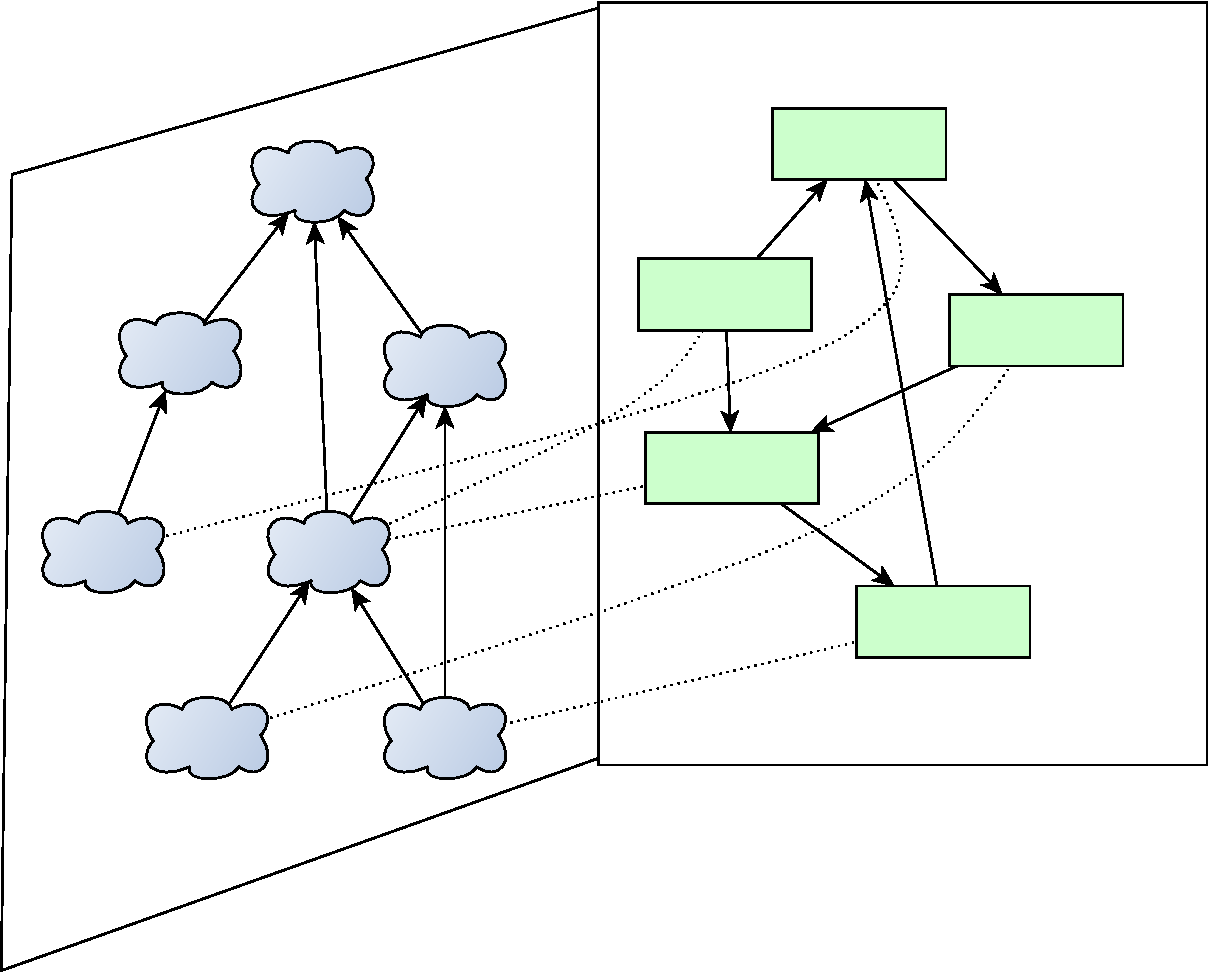
\includegraphics[width=0.8\textwidth]{illustrations/hierarchies-crop.pdf}
\caption{Иерархии классов и объектов}
\label{fig:hierarchies-crop}
\end{figure}

Проектирование хорошей иерархии это всегда сложный инженерный процесс, выходящий за рамки этого курса. Зато можно на игрушечных примерах рассмотреть основные проблемы, ожидающие разработчика на этом пути.

\subsection{Виртуальные функции при множественном наследовании}\label{VirtThunks}

При одиночном наследовании, отношение is-a, задаваемое открытым наследованием не вызывает проблем при использовании такой стандартной техники как таблицы виртуальных методов. На (рис. \ref{fig:multinh-crop}) изображена условная схема размещения в памяти объекта класса \lstinline!B!, определяемого как:

\begin{lstlisting}
class A { /* A part */ };
class B : public A { /* B part */ };
\end{lstlisting}

Видно, что указатель \lstinline!A*! в памяти указывает в точности туда же, куда \lstinline!B*! и одна и та же таблица виртуальных методов вполне достаточна.

\begin{figure}[h!]
\centering
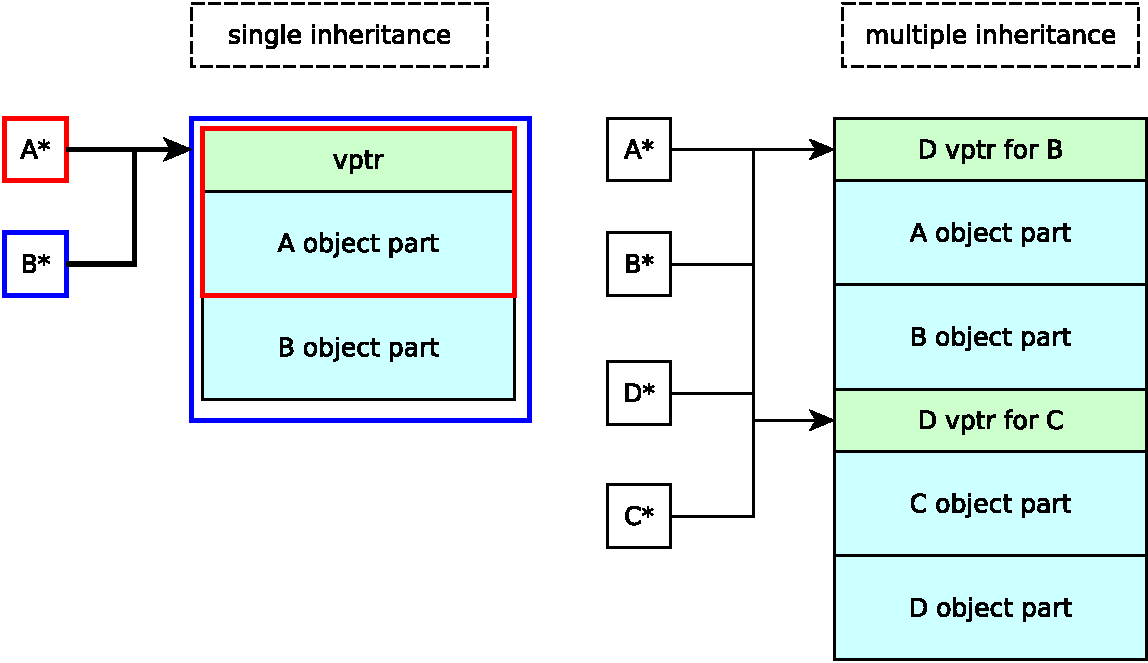
\includegraphics[width=1.0\textwidth]{illustrations/multinh-crop.pdf}
\caption{Виртуальные функции при множественном наследовании}
\label{fig:multinh-crop}
\end{figure}

Для прогулок по такой иерархии вполне достаточно статического приведения типа:

\begin{lstlisting}
B* ptrB = new B;
A* ptrA = ptrB;
ptrB = static_cast<B*>(ptrA);
\end{lstlisting}

Увы, для множественного наследования вечер резко перестаёт быть томным. Справа на (рис. \ref{fig:multinh-crop}) изображена ситуация, которая получается если добавить пару классов к иерархии:

\begin{lstlisting}
class C { /* C part */ };
class D : public B, public C { /* D part */ };
\end{lstlisting}

Даже если предположить, что две таблицы виртуальных функций будут совмещены, всё равно неясно куда должен показывать \lstinline!С*! если учесть, что в объекте после его разыменования или срезки просто не должно быть никаких частей от классов \lstinline!A! и \lstinline!B!, к которым он вообще не имеет отношения.

\begin{lstlisting}
D* ptrD = new D;
B* ptrB = ptrD;
A* ptrA = ptrD;
C* ptrC = ptrD; // Where to point?
\end{lstlisting}

К счастью стандарт регламентирует, что это не ваша головная боль, а головная боль компилятора. Компилятор статически знает, что при множественном наследовании преобразования некоторых типов на добавку постоянного смещения дороже, чем преобразования некоторых других типов (это безумие реализуется в бэкенде GCC через virtual function thunks -- специальные участки кода, в которых бэкенд решает сколько добавить к указателю при вызове виртуальной функции).

Теперь настало время разобраться с чем-то, что является \textbf{вашей} головной болью.

\subsection{Ромбовидные схемы и виртуальные базовые классы}\label{RombSchemas}

Предположим, вы проектируете систему, поддерживающую абстракции файлов ввода и вывода. Рано или поздно вы пришли к чему-то вроде такого

\begin{lstlisting}
class File {};
class InputFile : public File {};
class OutputFile : public File {};
class IOFile : public InputFile, public OutputFile {};
\end{lstlisting}

Графически это может быть выражено ромбовидной схемой

\begin{figure}[h!]
\centering
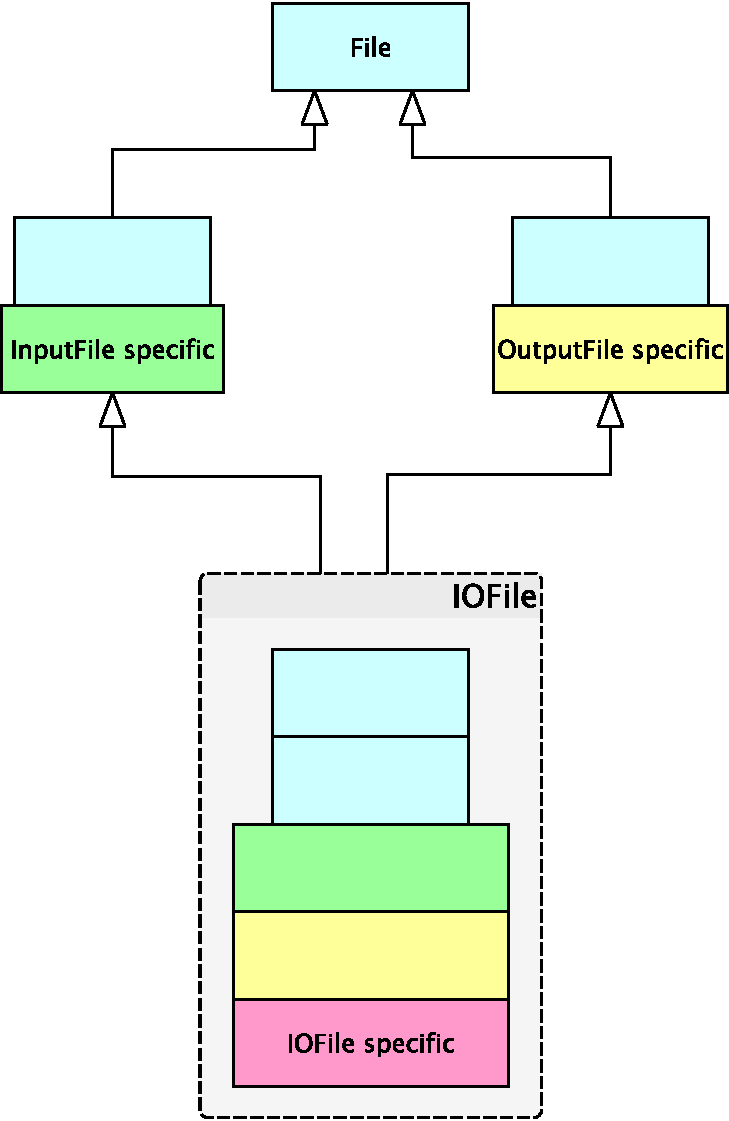
\includegraphics[width=0.5\textwidth]{illustrations/romb-crop.pdf}
\caption{Ромбовидная схема}
\label{fig:romb-crop}
\end{figure}

Предположим, что в классе \lstinline!File! есть поле \lstinline!File::filename!. По умолчанию, в классе \lstinline!IOFile! у вас получится два члена: \lstinline!InputFile::File::filename! и \lstinline!OutputFile::File::filename!, но файл у которого два имени это абсурд. 

Ещё хуже то, что отношение is-a похоже перестаёт работать в таких случаях:

\begin{lstlisting}
IOFile* iof = new IOFile;
File *f = iof; // Ooops!
\end{lstlisting}

Здесь абсолютно неясно на какую из двух частей \lstinline!InputFile::File! и \lstinline!OutputFile::File! теперь указывает \lstinline!f!. И вот это уже гораздо более серьёзная проблема, чем просто чуть больше оверхеда.

Прошаренный в C++ пацан предложил бы следующий способ устранения неоднозначности (disambiguation).

\begin{lstlisting}
File* outPtr = static_cast<OutputFile*>(iof);
File* inPtr = static_cast<InputFile*>(iof);
\end{lstlisting}

Но такие прекрасные хаки никак не спасают от фундаментальных проблем при вызове виртуальных функций. Если переопределение функции \lstinline!open! предлагается только классами \lstinline!File! и \lstinline!OutputFile!, что должно произойти при вызове \lstinline!inPtr->open!?

Чтобы избежать такой ситуации, базовый класс в наследовании может быть объявлен виртуальным (ещё можно вообще никогда ничего не писать на C++, а использовать C, это предпочтительный вариант).

\begin{lstlisting}
class File {};
class InputFile : virtual public File {};
class OutputFile : virtual public File {};
class IOFile : public InputFile, public OutputFile {};
\end{lstlisting}

Теперь всё хорошо и в ромбовидной схеме у самого нижнего производного класса есть только одна копия базового. В памяти это может выглядеть как-то так:

\begin{figure}[h!]
\centering
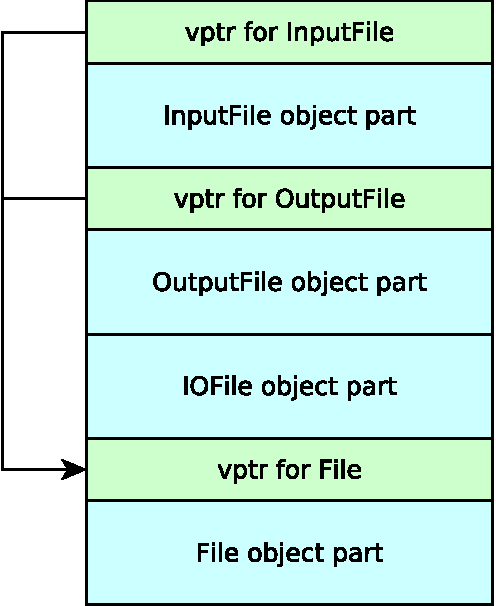
\includegraphics[width=0.5\textwidth]{illustrations/virtualinh-crop.pdf}
\caption{Виртуальное наследование}
\label{fig:virtualinh-crop}
\end{figure}

Таблицы виртуальных методов ещё более усложнились. Показанные стрелки позволяют во время исполнения как бы ``склеивать'' подобъекты, получая указатели на них.

\begin{lstlisting}
File* ptrF1 = ptrInputFile;
File* ptrF2 = ptrOutputFile;
File* ptrF3 = ptrIOFile;
\end{lstlisting}

Всё это будет работать и возвращать правильные (по крайней мере -- правильно себя ведущие) указатели. Увы, любое обращение по такому указателю связано уже с тремя уровнями косвенности: разрешение виртуального наследования, разрешение множественного наследования и далее собственно вызов по косвенности виртуального метода. Это указатель на указатель на указатель на функцию и, обычно, это высокий барьер для оптимизаций в компиляторе.

Ещё одна проблема -- виртуальное наследование отключает понижающие статические преобразования:

\begin{lstlisting}
IOFile* ptrIO = static_cast<IOFile*>(ptrF3); // Error
\end{lstlisting}

\textbf{Вопрос к студентам:} почему это происходит?

\ifanswers
Правильный ответ: потому что для реконструкции объекта с виртуальным наследованием, компилятор должен пройти по каждой из возможных цепочек виртуального наследования и создать каждый из подобъектов. Это неконстантный оверхед по времени и памяти и разработчики языка не стали его закладывать в обычное преобразование.
\fi

Для того, чтобы выполнять понижающее преобразование, следует воспользоваться специально введенным для этого в язык динамическим приведением типа.

\subsection{Динамическое приведение\index{dynamic\_cast} и RTTI\index{RTTI}}\label{DynCastRTTI}

Кроме всех операторов приведения, рассмотренных в (\ref{FromCCastToCPP}), существует ещё один, разработаный специально, чтобы приводить статический тип к динамическому типу. Он называется \lstinline!dynamic_cast!. 

Его интересной особенностью является то, что он по-разному работает для указателей и для ссылок. 

Для указателей

\begin{lstlisting}
Derived* temp = dynamic_cast<Derived*>(base);
\end{lstlisting}

Пытается привести p, типа \lstinline!Base*! к типу \lstinline!Derived*!, где \lstinline!Base! и \lstinline!Derived! принадлежат одной и той же иерархии. Если \lstinline!Derived! является базовым классом для \lstinline!Base!, то это ничем не отличается от \lstinline!static_cast!. Но \lstinline!dynamic_cast! работает также если Base является полиморфным базовым классом для \lstinline!Derived!, то есть является базовым классом для \lstinline!Derived! и содержит виртуальные функции. Звучит запутано? Давайте посмотрим пример.

\begin{lstlisting}
struct NamedObject {
  virtual const char *whoareyou() const = 0;
};
\end{lstlisting}

\begin{lstlisting}
struct Pokemon : NamedObject {
  const char *whoareyou() const { return "Pokemon"; }
};

struct DartVeider : NamedObject {
  const char *whoareyou() const { return "Dart Veider"; }
};
\end{lstlisting}

\begin{lstlisting}
int check_DartVeider(NamedObject *p)
{
  if (dynamic_cast<DartVeider *>(p))
    {
      printf("You are Dart Veider!\n");
    }
  else
    {
      printf("You are not Dart Veider, you are %s\n", p->whoareyou());
    }
  return 0;
}
\end{lstlisting}

\begin{lstlisting}
DartVeider dv;
Pokemon pm;
check_DartVeider(&dv);
check_DartVeider(&pm);
\end{lstlisting}

Что будет на выдаче? Ответ:

\begin{verbatim}
You are Dart Veider!
You are not Dart Veider, you are Pokemon
\end{verbatim}

Коротко говоря, \lstinline!dynamic_cast!, использованый для указателя даёт возможность ``спросить'' такой ли у этой переменной динамический тип, как он полагает. Он приводит к этому типу если ответ ``да'' или возвращает \lstinline!nullptr!, если ответ ``нет''.

При использовании \lstinline!dynamic_cast! для ссылок, вопрос превращается в утверждение. Если это утверждение нарушается, то выбрасывается исключение и без специальной обработки, программа будет завершена (подробнее про обработку таких ситуаций см. \ref{subsec:basicexceptions}).

\textbf{Вопрос к студентам:} может ли \lstinline!dynamic_cast! работать везде, где работает \lstinline!static_cast!?

\ifanswers
Правильный ответ: нет \lstinline!dynamic_cast! очень важно, чтобы в базовом классе была хотя бы одна виртуальная функция -- если таблицы виртуальных методов не будет существовать, динамическое приведение не будет работать.
\fi

Именно такой вид преобразования является законным понижающим преобразованием в виртуальных иерархиях.

\begin{lstlisting}
IOFile* ptrIO = dynamic_cast<IOFile*>(ptrF3); // Ok
\end{lstlisting}

Важно понимать: любое использование \lstinline!dynamic_cast! это легальный способ попросить компилятор сделать вашу программу гораздо медленнее и несколько больше по размеру. Дело в том, что для своей работы он использует запросы к так называемой run time type information или RTTI -- обычно это структура, привязанная к виртуальной таблице. Измерить (или хотя бы оценить) точный оверхед обращения к этой структуре и её хранения невозможно. Считается, что если вы используете \lstinline!dynamic_cast!, вы знаете что делаете.

Из опыта автора этих лекций, обычно люди, использующие его, вообще не знают что делают. Даже примерно.

\subsection{Информация о типах и идентификаторы типов\index{type\_info}}\label{TypeInfo}

Каждому типу в C++ соотнесен дескриптор, имеющий тип \lstinline!type_info!. Этот дескриптор для любого типа можно получить вызвовом функции \lstinline!typeid!. Такие объекты содержащие информацию о динамических типах можно сравнивать. Можно также, начиная с 2011, сравнивать их хеш-коды.

Таким образом, есть два варианта сравнения совпадает ли динамический тип с заданным.

\begin{enumerate}

\item Использовать dynamic cast

\begin{lstlisting}
if (dynamic_cast<A*> someVar != 0) { 
  //it is of class A, or X, inherited from A 
}
\end{lstlisting}

\item Использовать typeid

\begin{lstlisting}
if (typeid(someVar) == typeid(A)) {
   //it is of class A
}
\end{lstlisting}

\end{enumerate}

Первый способ позволяет сравнить нечетко, динамический тип может быть приведен к \lstinline!A! из любого наследника. Во втором случае сравнение будет четким, а главное -- дешевым. Сравнить идентификаторы типов имеет постоянную сложность. Динамическое приведение типов требует обхода деревьев RTTI и может работать непредсказуемо долго.

\textbf{Вопрос к студентам:} зачем же вообще нужен \lstinline!dynamic_cast! если есть \lstinline!typeid!?

\ifanswers
Правильный ответ: в первую очередь из-за сложностей приведения в связке \lstinline!typeid! + \lstinline!static_cast! (см. выше разговор о том почему в иерархиях множественного наследования нам вообще не хватает статического приведения).
\fi

\subsection{Сюрпризы в конструкторах при виртуальном наследовании}\label{VirtualBaseClassConstr}

Пусть виртуальный базовый класс имеет нетривиальный конструктор как в (\ref{BaseClassConstr}).

\begin{lstlisting}
class A 
{
  int x_;
public:
  A(int x) : x_(x) {}
};
\end{lstlisting}

И является виртуальным базовым для классов:

\begin{lstlisting}
// C is similar
struct B : virtual public A {
  B(int x):A(x){}
};
\end{lstlisting}

Увы, ожидаемый порядок конструирования для класса наследующего по ромбовидной схеме не сработает интуитивно:

\begin{lstlisting}
struct D : public B, public C {
  D(int x) : B(x), C(x) {} // Error!
}
\end{lstlisting}

Дело в том, что виртуальный базовый класс должен быть обязательно сконструирован в самом нижнем наследнике, то есть:

\begin{lstlisting}
  D(int x) : A(0), B(x), C(x) {} 
\end{lstlisting}

Мало того, подобъект A будет сконструирован именно с параметром 0, те параметры, которые передаются к общей базе через конструкторы подобъектов B и C, будут проигнорированы.

Это распространяется и ниже по иерархии туда, где об общем виртуальном предке все уже давно забыли:

\begin{lstlisting}
struct E : public D {
  E() : D(10) {} // Error!
};
\end{lstlisting}

Теперь самый нижний класс в иерархии внезапно \lstinline!E!. Это значит, что виртуально-базовая часть должна быть сконструирована в нем.

\subsection{Порядок инициализации в сложных диаграммах}\label{InitOrder}

Важно очень хорошо представлять себе порядок конструирования сложных диаграмм классов. Ниже приведен несколько синтетический (но на самом деле гораздо менее сложный, чем многие практически важные иерархии) пример.

\begin{lstlisting}
class B1 { };
class V1 : public B1 { };
class D1 : virtual public V1 { };
class B2 { };
class B3 { };
class V2 : public B1, public B2 { };
class D2 : virtual public V2, public B3 { };
class M1 { };
class M2 { };
class X : public D1, public D2 {
  M1 m1_;
  M2 m2_;
};
\end{lstlisting}

Для простоты можно изобразить эту иерархию на листочке:

\begin{figure}[h!]
\centering
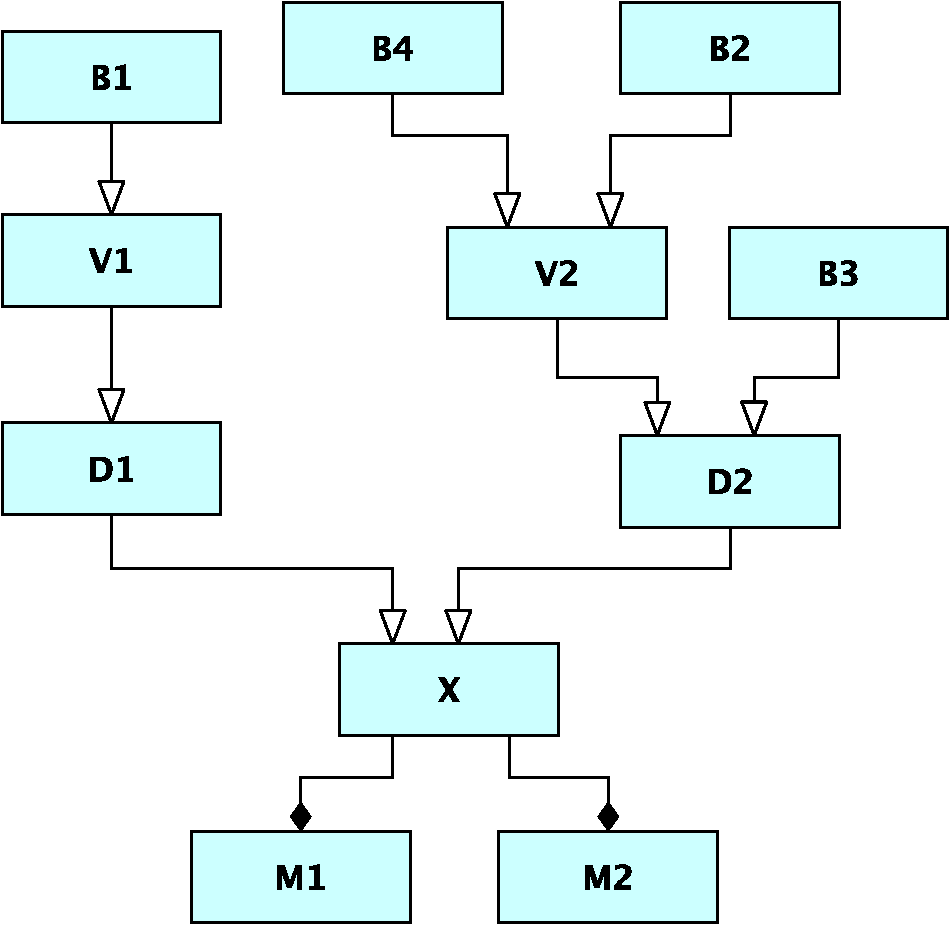
\includegraphics[width=0.5\textwidth]{illustrations/complexhier-crop.pdf}
\caption{Сложная иерархия}
\label{fig:complexhier-crop}
\end{figure}

Порядок инициализации объекта класса \lstinline!X! для изображённой иерархии следующий:

\begin{itemize}
\item Сначала конструируются виртуальные базовые классы
  \begin{enumerate}
  \item Конструирование \lstinline!V1!: \lstinline!B1::B1()!, \lstinline!V1::V1()!
  \item Конструирование \lstinline!V2!: \lstinline!B1::B1()!, \lstinline!B2::B2()!, \lstinline!V2::V2()!
  \end{enumerate}
\item Затем конструируются невиртуальные базовые классы
  \begin{enumerate}
  \item Конструирование \lstinline!D1!: \lstinline!D1::D1()!
  \item Конструирование \lstinline!D2!: \lstinline!B3::B3()!, \lstinline!D2::D2()!
  \end{enumerate}
\item Затем конструируются члены \lstinline!M1::M1()!, \lstinline!M2::M2()!
\item И в последнюю очередь выполняется конструктор \lstinline!X::X()!
\end{itemize}

Вид наследования (открытое, закрытое или защищённое) не влияет на порядок инициализации.

\subsection{Делегация сестринскому типу}

Сложности, вносимые множественным наследованием в работу механизма виртуальных функций, частично окупаются теми возможностями, которые они предоставляют.

Пусть задана ромбовидная иерархия, в которой виртуальная функция определена в одной, но не в другой ветке:

\begin{lstlisting}
struct VBase {
  virtual void foo () = 0;
  virtual void bar () = 0;
  virtual ~VBase () = 0 {}
};

struct Base1 : virtual public VBase {
  // do not override bar
  // but CALL it
  void foo() override { bar(); }  
};

struct Base2 : virtual public VBase {
  void bar() override {}
};

struct S : Base1, Base2 {}
\end{lstlisting}

На что может рассчитывать пользователь такого класса, вызывая метод \lstinline!foo! объекта класса \lstinline!S!?

\begin{lstlisting}
S x;
x.foo();
\end{lstlisting}

Происходит интересная вещь: поскольку метод \lstinline!foo! не переопределен в классе \lstinline!Base2!, будет без вариантов вызван метод \lstinline!Base1::foo!, который внезапно далее вызовет \lstinline!Base2::bar!. Несмотря на то, что классы \lstinline!Base1! и \lstinline!Base2! находятся на одном уровне, механизм виртуальных функций позволяет такие братские (ну или сестринские) делегации.

\subsection{Вложенные классы и снова о пространствах имён}\label{InnerClasses}

Вложенные функции в C++ невозможны так же как и в C (что кстати не вполне логично, так как вложенные лямбда-функции в новом стандарте возможны и будут рассмотрены на следующих лекциях, так что казалось бы гулять так гулять). Зато C++ позволяет вкладывать классы. Синтаксис очевиден, но, если необходимо, чтобы вложенный класс ``знал'' о своём окружении, об этом надо позаботиться отдельно:

\begin{lstlisting}
class DeathStar {
  DartVeider m_dv;
  const char *m_name;
public:
  DeathStar(const char *name) : m_name(name) {
    m_dv.starptr = this;
  }

  struct DartVeider {
    void whoareyou() const{
      auto where = starptr ? starptr->m_name 
                           : "hmm... I don't know where";
      std::cout << "I am Dart Veider, flying on " 
                 << where << std::endl;
        }
    DeathStar *starptr;    
  };

  void ask_dart_veider() const { m_dv.whoareyou(); }
};
\end{lstlisting}

Используется это как-то так.

\begin{lstlisting}
DeathStar d("Old Good Death Star");
d.ask_dart_veider();
\end{lstlisting}

Каждый вложенный класс определяет область видимости своих имён. Это позволяет гибко разграничивать уровень доступа в зависимости от архитектуры системы.

\pagebreak
\section{Скажи мне кто твой друг}\label{WhosYourFriend}\index{Friend}

\hfill\textit{C++ : Where friends have access to your private members}{\vspace{0.5em}}

\hfill\textit{-- Gavin Russell Baker}

Модель инкапсуляции C++ логична и стройна (общий смех). В общем случае закрытые члены класса формируют его состояние и недоступны извне, иначе, чем через его методы, отражающие поведение -- это хорошо и правильно. Но в некоторых случаях, разработчик хотел бы дать некоему классу эксклюзивный доступ к закрытым членам другого класса. Например для того, чтобы не писать кучу геттеров и в то же время сохранить консистентность абстракции. Для этого язык C++ предусматривает механизм друзей (\lstinline!friend!) класса.

\subsection{Обычная дружба}

Наиболее типичным применением дружбы является дружба между классами. Для этого объявление класса, которому хочется открыть внутреннее состояние должно быть предварено ключевым словом \lstinline!friend!.

\begin{lstlisting}
class Node {
  int data;
  int key;
  /* ..... */

  /* class BinaryTree can access data directly */
  friend class BinaryTree; 
};
\end{lstlisting}


Класс \lstinline!Node!, назначив себе друга \lstinline!BinaryTree!, открыл ему всё свое закрытое состояние, но, при этом, сам не получил никакого доступа к \lstinline!BinaryTree!. Теперь внутри BinaryTree можно написать код вида:

\begin{lstlisting}
class BinaryTree {
  Node *root;

public:
  int find(int key);
};

int BinaryTree::find(int key) {
  // check root
  if(root->key == key) {
    // no need to go through an accessor function
    return root->data;
  }
  // rest of find
}
\end{lstlisting}


Класс может открывать своё состояние не только классам, но и функциям. Скажем, не открывая доступ всему \lstinline!BinaryTree!, можно открыть его только методу \lstinline!find!:

\begin{lstlisting}
class Node {
  int data;
  int key;
  // ........

  // BinaryTree::find can access data directly
  friend int BinaryTree::find();
};
\end{lstlisting}

Открыть внутреннее состояние можно и отдельной функции. Как дополнительный плюс -- в этом случае функция считается объявленной.

\begin{lstlisting}
struct Node {
  // declaration
  friend int find();
};


// find declared and can be used
int t = find();

// definition
int find() {
  /* ..... */
}
\end{lstlisting}

Благодаря такому свойству объявлений, дружба может быть полезна во многих неожиданных контекстах при работе с шаблонами (см. \ref{BartonNackman}).

\subsection{Адвокат дружбе не помеха}

К сожалению, в языке не реализовано полноценное открытие части состояния. Семантика дружбы диктует ``все или ничего''. Но редко когда нужно, чтобы друзья имели доступ ко всему подряд. Пусть рассмотренный выше класс \lstinline!Node! согласен открыть классу \lstinline!BinaryTree! только свои поля \lstinline!data! и \lstinline!key!, оставив все остальные закрытыми. В этом случае классу \lstinline!Node! следует прибегнуть к услугам адвоката (английское слово attorney означает скорее ``поверенный'').

Игра слов даёт название идиоме attorney-client (адвокат-клиент). Адвокат, которым мог бы обзавестить \lstinline!Node! может выглядеть вот так

\begin{lstlisting}
class NodeAttorney {
private:
  static int& data(Node &c) {
    return c.data;
  } 
  static int& key(Node &c) {
    return c.key;
  } 
  friend class BinaryTree;
};
\end{lstlisting}

Теперь внутри \lstinline!Node! можно оставить только объявление дружбы со своим адвокатом, прочие же объявления дружбы вынести в класс, выполняющий роль attorney.

Особо параноидальный дизайн иерархии классов может предоставлять много адвокатов на каждое закрытое поле популярного клиента, каждого со своим списком пользователей.

Нужно очень хорошо понимать, что все эти игры свидетельствуют о наличии некоей проблемы между креслом и компьютером.

\subsection{Дружба в иерархиях классов}

Дружба не наследуется, но друг статического родительского типа достаточен, чтобы делать дружественные вызовы полиморфных наследников.

\begin{lstlisting}
class Parent
{
    friend class Family;
    protected:
        virtual void Answer() = 0;
};
\end{lstlisting}

\begin{lstlisting}
class Child : public Parent
{
  private:
    void Answer() { printf("Child!\n"); }
};
\end{lstlisting}

\begin{lstlisting}
class Family
{
friend class Parent;
public:
  void ParentAnswer(Parent *p) { p->Answer(); } // OK
  void ChildAnswer(Child *c) { c->Answer(); }  // FAIL
};
\end{lstlisting}

\begin{lstlisting}
Child c;
Family f;
f.ParentAnswer(&c); /* ok */
\end{lstlisting}

В общем случае, дружба статических типов вредна для инкапсуляции. Но дружба, позволяющая полиморфные вызовы по большой и закрытой иерархии это полезно и иногда необходимо. 

\subsection{Дружба и виртуальные вызовы}

Часто хочется, чтобы функция-друг была виртуальной. К сожалению это невозможно, так как в таблице виртуальных методов на друзей нет места, к тому же у друзей нет неявного полиморфного аргумента, так что они не могут быть полиморфными функциями.

Предположим, что функция \lstinline!find! должна уметь работать как с \lstinline!Node! так и с его потомками.

\begin{lstlisting}
class Node
{
public:
  friend int find(Node& n);
};

class SparceNode : public Node
{
public:
  friend int find(Node& n);
};

SparceNode t;
find(t); // oops, we shall use 
         // another approach here
\end{lstlisting}

Классическим выходом из положения (чем-то напоминающим идиому NVI) является реализация такой функции через закрытую действительно виртуальную функцию.

\begin{lstlisting}
class Node
{
protected:
  virtual int find();
public:
  friend int find(Node& n);
};

class SparceNode : public Node
{
protected:
  virtual int find();
public:
  friend int find(Node& n);
};

int find(Node& n) {
  return n.find(); // virtual call
}

SparceNode t;
find(t); // ok
\end{lstlisting}

Идея здесь в том, что каждый класс знает как лучше искать свои объекты, а общая функция друг выполняет роль прозрачного интерфейса.

\pagebreak
\section{Основные принципы ООП}\index{SOLID}\label{SOLID}

\hfill\textit{Design and programming are human activities;}

\hfill\textit{forget that and all is lost}{\vspace{0.5em}}

\hfill\textit{-- Bjarne Stroustrup}

При использовании объектно ориентированного программирования, на практике оказывается полезным придерживаться некоторых принципов.

\subsection{Принцип единственной обязанности}\index{SRP}\label{SRP}

Не только классы и объекты занимаются инкапсуляцией данных. На языке C, данные могут быть инкапсулированы в модуль (объявлены в нём статическими переменными и функциями) и программист, использующий такой модуль, будет оперировать только его открытым интерфейсом. Данные могут быть инкапсулированы и в обычных функциях, когда локальные переменные внутри функции безопасны относительно изменений извне. Общее понятие, определяющее совокупность ``своих'' данных, используемых для неких ``своих'' целей называется \textbf{контекст}.

Принцип единственной обязанности гласит, что для каждого контекста следует выделять единственную обязанность и полностью инкапсулировать всё, относящееся к деталям её выполнения.

Пример плохого проектирования:

\begin{lstlisting}
class IEmail {
public:
  virtual void setHeader (string smtp_header) = 0;
  virtual void setContent (string plaintext_content) = 0;
  virtual void send (string Receivers) = 0;
};
\end{lstlisting}

Здесь у класса три области ответственности: он определяет протокол, контент и отсылку письма. Гораздо лучше дать возможность использовать разные виды протоколов и разные виды контента

\begin{lstlisting}
class IContent;
class IHeader;

class IEmail {
public:
  virtual void setHeader (IHeader *header) = 0;
  virtual void setContent (IContent *content) = 0;
  virtual void send (string Receivers) = 0;
};
\end{lstlisting}

Основная интенция принципа единственной обязанности: у каждого класса должна быть только одна причина для изменения. На этапе проектирования этот принцип помогает думать о возможных расширениях проекта и правильно разбивать проект на легко модифицируемые взаимодополняющие классы.

\subsection{Принцип открытости и закрытости}\index{OCP}\label{OCP}

В своей простейшей формулировке он звучит так: ``каждый контекст должен быть открыт для расширения, но закрыт для изменения''. Это означает, что при наличии контекста, корректно выполняющего одну обязанность, разработка контекста, выполняющего обязанность, которая расширяет данную, исходный код первого контекста должен быть переиспользован, но не изменен. Это особенно значимо в производственной среде, когда изменения в исходном коде потребуют проведение пересмотра кода, модульного тестирования и других подобных процедур, чтобы получить право на использования его в программном продукте. Код, подчиняющийся данному принципу, не изменяется при расширении и поэтому не требует таких трудозатрат.

Пример нарушения:

\begin{lstlisting}
class IScreen {
  void drawRectangle ();
  void drawCircle ();
  void drawLine ();
public:
  enum shape {RECTANGLE, CIRCLE, LINE};
protected:
  shape m_shape;
public:
  void draw (shape x);  
};
\end{lstlisting}

Этот контекст в абсолютной степени открыт для изменения (оно мало того необходимо при попытке добавить любую функциональность), но закрыт для расширения. Должно быть наоборот:

\begin{lstlisting}
class IFigure;
class IRectangle: public IFigure;
// ..... etc
class IScreen {
public:
  void draw (IFigure *f);
};
\end{lstlisting}

Теперь при необходимости расширения, достаточно унаследовать новый класс от общего интерфейса.

\subsection{Принцип подстановки Лисков}\index{LSP}\label{LSP}

И реализация интерфейса и открытое наследование реализации это на самом деле одно и то же фундаментальное отношение, которое в англоязычной литературе называется ``is-a'', а по-русски -- специализацией (не стоит путать с шаблонной специализацией, это очень разные вещи, здесь термин употреблен в логическом смысле как сужение объёма понятия). Есть некая терминологическая несогласованность в том, как называть классы выше и ниже по иерархии наследования. Многие из предлагаемых в современной литературе вариантов, ``родитель'' и ``наследник'', или, скажем, ``суперкласс'' и ``подкласс'', кажутся вводящими в заблуждение. Далее классы, стоящие выше по иерархии, будут называться \textbf{базовыми} для классов, стоящих ниже, а классы стоящие ниже в иерархии -- \textbf{производными} от стоящих выше.

Отношение обобщения и специализации в правильно спроектированной иерархии классов должно подчиняться ``принципу подстановки''. 

Этот принцип, сформулированный Барбарой Лисков в \cite{LSP}, гласит, что любое свойство объектов базового класса должно быть верно и для объектов производного класса. Иначе говоря, любая функция, работающая с объектом базового класса, должна работать и с любым объектом производного класса. Поскольку удовлетворящий LSP наследник может быть \textbf{подставлен} в контекст, где использован базовый класс, этот принцип называется принципом подстановки.

Самый простой пример нарушения принципа подстановки -- перегрузка виртуальных функций базового класса невиртуальными функциями наследника. Более сложные примеры его применения будут рассмотрены в (\ref{InhProblems}).

\subsection{Принцип разделения интерфейса}\index{ISP}\label{ISP}

Самая простая его формулировка была дана Робертом Мартином в \cite{ISP} и звучит так: ``Клиенты не должны зависеть от методов, которые они не используют''

Принцип разделения интерфейсов говорит о том, что слишком ``толстые'' интерфейсы необходимо разделять на более маленькие и специфические, чтобы клиенты маленьких интерфейсов знали только о методах, которые необходимы им в работе. В итоге, при изменении метода интерфейса не должны меняться клиенты, которые этот метод не используют.

Пример нарушения:

\begin{lstlisting}
class IWorker {
  virtual public void work() = 0;
  virtual public void eat() = 0;
};

class Manager {
  IWorker *m_w;
public:
  Manager(IWorker *w):m_w(w){}
  void manage() {
    m_w->work();
  }
};
\end{lstlisting}

В этом исключительно сложном, но жизненном примере менеджер реально пользуется только способностью рабочего работать. Но он зависит от интерфейса в котором также включена не используемая им возможность есть. Скажем теперь разработчик решил ввести \lstinline!class Robot: public Worker!. Что делать с абсолютно лишним для робота интерфейсом? Ну скажем можно установить ланч длиной в одну секунду (плохая идея). Гораздо лучше:

\begin{lstlisting}
class IWorkable {
  virtual public void work() = 0;
};

class IFeedable {
  virtual public void eat() = 0;
};

class IWorker : public IWorkable, public IFeedable;

class Manager {
  IWorkable *m_w;
// ..... etc
};
\end{lstlisting}

Здесь интерфейс разделен и класс менеджера больше не зависит от не используемых им особенностей рабочей силы

\subsection{Принцип инверсии зависимостей}\index{DIP}\label{DIP}

Обычный способ думать о зависимостях между модулями -- это рассмотрение зависимостей высокоуровневых модулей от низкоуровневых. Принцип инверсии разворачивает зависимость и гласит, что:

\begin{enumerate}
\item Модули верхних уровней не должны зависеть от модулей нижних уровней. Оба типа модулей должны зависеть от абстракций.
\item Абстракции не должны зависеть от деталей. Детали должны зависеть от абстракций.
\end{enumerate}

\subsection{Закон Деметры}\index{Demeter Law}\label{DemeterLaw}

Перечисленные выше пять принципов входят в пятёрку SOLID, предложенную Робертом Матрином. Кроме SOLID-принципов, известны другие, в частности Закон Деметры, который гласит: ``Объект A не должен иметь возможность получить непосредственный доступ к объекту C, если у объекта A есть доступ к объекту B и у объекта B есть доступ к объекту C''. Чтобы понять его совсем просто, можно сказать ``Наездник должен управлять лошадью, а не ногами лошади''.

Преимуществами закона Деметры является то, что код, разработанный с соблюдением данного закона, делает написание тестов более простым, а разработанное программное обеспечение менее сложно при поддержке и имеет большие возможности повторного использования кода. Так как объекты являются менее зависимыми от внутренней структуры других объектов, контейнеры объектов могут быть изменены без модификации клиентов.

\subsection{Проблемы, возникающие при проектировании открытого наследования}\label{InhProblems}

Принцип подстановки Лисков требует навыка при работе с ним. Предположим, вы проектируете иерархию геометрических объектов и столкнулись с необходимостью расположить в ней такие абстракции как ``квадрат'' и ``прямоугольник''. Первой мыслью может быть унаследовать прямоугольник от квадрата – в конце концов прямоугольник вводит ещё одно поле и может быть какие-нибудь дополнительные методы

\begin{lstlisting}
class Square {
public:
  Square(double x) : m_x(x) {}
  virtual ~Square() {}
  double a() const { return m_x; }
  virtual double get_sq() const { return a() * a(); }
protected:
  double m_x;
};

class Rect: public Square {
public:
  Rect(double x, double y) : Square(x), m_y(y) {}
  int b() const { return m_y; }
  double get_sq() const override { return m_x * m_y; }
private:
  double m_y;
};
\end{lstlisting}

Но такой подход создаёт проблемы, связанные с тем, что прямоугольник не является частным случаем квадрата и здесь нарушается принцип подстановки. 

\textbf{Домашняя наработка:} опишите проблемы которые может вызвать такое проектирование. Например рассмотрите реализованную в \lstinline!Square! (и даже виртуальную) функцию \lstinline!void increase(int times)!, в times раз увеличивающую площадь квадрата. Как вы реализуете её для прямоугольника?

\pagebreak
\section{Паттерны объектно-ориентированного программирования}\label{DesPatterns}

\hfill\textit{If you want to sell a cat to a computer scientist}

\hfill\textit{you have to tell him it's object-oriented}{\vspace{0.5em}}

\hfill\textit{-- Roger King}

Введенные в 1995 году в книге \cite{DPatterns}, паттерны проектирования получили заслуженную популярность в инженерной среде как простой и впечатляющий способ говорить об архитектуре на понятном для посвященных языке.

Авторы предлагали классифицировать паттерны по двум критериям: цели и уровню. По цели паттерны делятся на порождающие, структурные и поведенческие, а по уровню -- на уровня класса и уровня объекта. Но классификация по уровню на самом деле довольно условна (особенно в языках с развитым метапрограммированием), поэтому ниже паттерны класифицированы по цели.

\subsection{Порождающие паттерны}

Наиболее популярные из порождающих паттернов -- Фабричный метод и Абстрактная фабрика по сути уже были рассмотрены. Это (с разных сторон) идиома виртуального конструктора в C++ (см. \ref{VirtCtors}). Паттерн Prototype это виртуальный копирующий конструктор и его рассмотрение оставлено на самостоятельную работу в рамках домашнего задания.

Ещё один паттерн из числа порождающих -- печально известный синглтон (Singleton). Увы, это скорее антипаттерн, так как нет почти никаких отличий синглтонов от глобальных переменных.

Поэтому здесь будет рассмотрен менее известный и одиозный, но прекрасно применимый паттерн Builder. Он находит применение во всех случаях, когда необходимо создавать сложно параметризованные объекты. Например в кодогенераторе компилятора, программист может захотеть создавать инструкцию по мнемонике и аргументам. Проблема в том, что конкретное соответствие аргументов с мнемоникой это деталь реализации бэкенда. Так например в конкретной архитекутре могут быть сложение с тремя или четырьмя аргументами, логические инструкции с двумя или тремя аргументами или даже некие мнемоники с большим количеством аргументов и странным смыслом.

Желаемый синтаксис, который даёт максимальную гибкость, можно представить следующим образом.

\begin{lstlisting}
// we want ADD R0, R1, 1
MachineInstrBuilder NewMIB(ADD);
NewMIB.addReg(R0);
NewMIB.addReg(R1);
NewMIB.addImm(1);
MachineInstr *NewMI = NewMIB.get();
\end{lstlisting}

Здесь \lstinline!MachineInstrBuilder! это класс-строитель, который принимает в конструкторе мнемонику и дальше через серию своих методов, таких как \lstinline!addReg!, \lstinline!addImm!, \lstinline!addLabelRef!, \lstinline!addMem! и так далее позволяет создавать сколь угодно причудливые варианты машинных инструкций. В конце метод \lstinline!get! может проверять существует ли на самом деле в описании архитектуры созданная инструкция и возвращать \lstinline!nullptr! (или делать нечто более сложное), если нет.

\subsection{Структурные паттерны}

Паттерны Адаптер, Декоратор, Приспособленец и Фасад понятны из названия, не отличаются разнообразием и обычно свидетельствуют о плохой архитектуре.

В качестве интересного структурного паттерна можно рассмотреть паттерн Мост. Этот паттерн позволяет протянуть связь между абстракцией и интерфейсом реализации. При этом тем же мостом могут пользоваться уточненные абстракции, создавая для себя улучшенных реализаторов.

Пусть речь идёт о планировании (scheduling) исполняемого кода -- одной из последних фаз оптимизатора. Каждый планировщик работает по своему алгоритму: жадному или основанному на расчистке критического пути и так далее. Кроме того, планировщик может быть локальным или глобальным. Паттерн мост позволяет развязать друг с другом конкретный интерфейс и конкретную реализацию, как это показано на (рис. \ref{fig:bridge_pattern}).

\begin{figure}[h!]
\centering
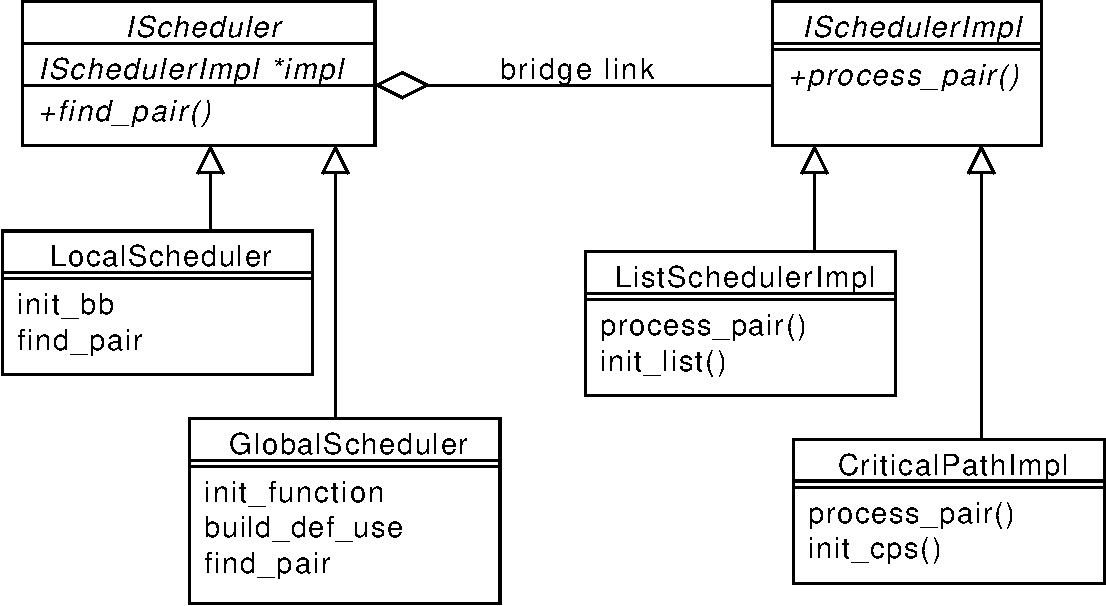
\includegraphics[width=0.8\textwidth]{illustrations/sched-bridge-crop.pdf}
\caption{Паттерн Bridge}
\label{fig:bridge_pattern}
\end{figure}

Благодаря абстрактному интерфейсу скрывающему реализацию, в этом примере также выполняется ISP.

\subsection{Паттерны поведения}

Паттерны поведения -- самый интересный раздел, среди них интересны почти все. Например при рассмотрении стандартной библиотеки, будет рассмотрено использование паттерна Итератор (для итераторов) и паттерна Стратегия (для аллокаторов). В качестве характерного примера поведенческих паттернов здесь можно рассмотреть паттерн Наблюдатель.

Этот паттерн позволяет как бы ``подписать'' один объект на уведомления другого. Пусть объект, который содержит данные будет простым и не содержит ничего кроме целого числа (и вектора наблюдателей).

\begin{lstlisting}
class Subject {
    vector < class Observer * > views; 
    int value;
  public:
    void attach(Observer *obs) {
        views.push_back(obs);
    }
    void setVal(int val) {
        value = val;
        notify();
    }
    int getVal() {
        return value;
    }
    void notify();
};
\end{lstlisting}

В функции \lstinline!notify! также нет ничего сложного: она просто уведомляет всех наблюдателей о смене состояния.

\begin{lstlisting}
void Subject::notify() {
  for (int i = 0; i < views.size(); i++)
    views[i]->update();
}
\end{lstlisting}

Теперь нужно договориться что наблюдают наблюдатели. Предположим, что частное или остаток от деления числа субъекта на заданное число (в реальных программах все будет сложнее, но это учебный пример).

Общий класс задает виртуальный метод \lstinline!update! для реализации в подклассах.

\begin{lstlisting}
class Observer {
    Subject *model;
    int denom;
  public:
    Observer(Subject *mod, int div) {
        model = mod;
        denom = div;
        model->attach(this);
    }
    virtual void update() = 0;
  protected:
    Subject *getSubject() {
        return model;
    }
    int getDivisor() {
        return denom;
    }
};
\end{lstlisting}

Теперь два подкласса.

\begin{lstlisting}
class DivObserver: public Observer {
  public:
    DivObserver(Subject *mod, int div): Observer(mod, div){}
    void update() {
        int v = getSubject()->getVal(), d = getDivisor();
        cout << v << " div " << d << " is " << v / d << '\n';
    }
};

class ModObserver: public Observer {
  public:
    ModObserver(Subject *mod, int div): Observer(mod, div){}
    void update() {
        int v = getSubject()->getVal(), d = getDivisor();
        cout << v << " mod " << d << " is " << v % d << '\n';
    }
};
\end{lstlisting}

Все это складывается вместе вот в такую замечательную городушку.

\begin{lstlisting}
int main() {
  Subject subj;
  DivObserver divObs1(&subj, 4);
  DivObserver divObs2(&subj, 3);
  ModObserver modObs3(&subj, 3);
  subj.setVal(14);
}
\end{lstlisting}

\textbf{Вопрос к студентам:} и что будет на экране?

\ifanswers
Правильный ответ: частное от деления 14 на 4 это 3, на 3 это 4 и в обоих случаях 2 в остатке. Так что 3, 4, 2.
\fi

\pagebreak
\section{Домашняя наработка по ООП}

\textbf{Контрольные вопросы}

\begin{enumerate}
\item Может ли нестатический метод в структуре вызывать статический метод?
\item Можно ли создать объект класса в конструкторе этого класса?
\item Можно ли создать объект класса в деструкторе этого класса?
\item Имеет ли смысл ключевое слово explicit для конструктора без аргументов?
\item Достаточно ли объявление класса для использования указателей на его методы?
\item Почему у конструкторов и деструкторов нет возвращаемых значений?
\item Можно ли перегрузить деструктор (так же как мы перегружаем конструкторы)?
\item Назовите оба способа задать неявное преобразование типов для вашего класса.
\item В лекциях рассмотрены const методы. Бывают ли volatile методы классов?
\item Может ли возникнуть необходимость объявить поле одновременно const и mutable?
\item Чем отличается указатель на статический метод от указателя на нестатический?
\item Что означает сокращение RAII, зачем нужна эта идиома?
\item Чем плоха идея реализовать копирующий конструктор через вызов оператора присваивания к *this?
\item Может ли быть скопирован по умолчанию объект класса с полем-ссылкой?
\item Что означает сокращение RVO, для чего используется?
\item Чем плоха идея перегрузить фигурные скобки (наравне с квадратными и круглыми)?
\item В лекциях рассматриваются операторы new и sizeof. Почему это операторы, а не функции?
\item Сохраняется ли правая ассоциативность при переопределении += или -=? Почему да или почему нет?
\item Возможно ли переопределить правый декремент для классов с запрещенным копированием?
\item Перечислите стандартные и пользовательские формы new и delete
\item В каких случаях деструктор нужно вызывать явно?
\item Можно ли вызвать (тем или иным способом) конструктор класса?
\item Как выбрать между правой и константной левой ссылкой?
\item Есть ли смысл в константных правых ссылках?
\item В лекциях рассмотрено связывание левой ссылки с правой (класс RefBind). Возможно ли связывание в обратном направлении?
\item Как выбрать между конструктором копирования и перемещения?
\item Зачем в языке и std::move и std::forward если оба это просто static cast?
\item За счет каких механизмов языка мы можем использовать универсальные ссылки?
\item Работает ли std::forward для идеального проброса правых ссылок?
\item Как привести указатель на объект производного класса к ссылке на объект базового?
\item Во сколько обычных вызовов по косвенности может обойтись вызов виртуальной функции?
\item Можно ли получить указатель на чисто виртуальную функцию?
\item В C++ нет статических деструкторов. Если бы они были, что мог бы делать виртуальный статический деструктор?
\item Может ли виртуальная функция быть статической? А чисто виртуальная?
\item Зачем нужны виртуальные деструкторы?
\item Может ли виртуальная функция быть объявлена inline?
\item Возможно ли корректно скопировать производный класс по указателю на базовый?
\item Что такое проблема срезки и как она проявляется?
\item Что обозначает аббревиатура NVI, зачем нужна эта идиома?
\item Могут ли в чисто виртуальных функциях быть аргументы по умолчанию?
\item В чем отличия композиции от закрытого наследования?
\item Чем отличается виртуальное наследование от невиртуального?
\item Имеют ли смысл виртyальные базовые классы при одиночном наследовании?
\item Почему виртуальное наследование отключает понижающий static cast по иерархии?
\item У вас есть выбор между использованием dynamic cast и typeid для проверки типа, в каком случае чем вы воспользуетесь?
\item Расшифруйте аббревиатуру SOLID и объясните кратко каждую из входящих в неё аббревиатур.
\item Что такое закон Деметры?
\item Выберите любой из классических паттернов проектирования и объясните его применимость.
\end{enumerate}

\textbf{Задания}

\begin{enumerate}
\item
Расширьте код игры в мяч до трёхмерной 

\item
Введите в код игры в мяч примитивы синхронизации чтобы его можно было запускать в многопоточном окружении

\item
Расширьте код до игры в мяч со смещающимся центром тяжести (допустим мяч наполовину заполнен водой или песком)

\item
Разработайте конкретный класс \lstinline!CTime!, предназначенный для хранения текущего времени и вычисления временных интервалов. Не ограничивайтесь unix time, сделайте возможным, например, подсчёт количества часов от Куликовской битвы до Бородинского сражения

\item
Как можно улучшить рассмотренный в (\ref{RAII}) класс CFile? Реализуйте и протестируйте обёртку.

\item
Разработайте и реализуйте иерархию классов, для управления сетевым соединением. Предусмотрите как минимум классы для TCP и UDP сокетов, наследующие от общего предка

\item
Реализуйте абстрактный интерфейс материальной точки и унаследуйте от него разные варианты мяча -- идеальный, с сопротивлением воздуха, со смещённым центром тяжести, etc. На основе общего интерфейса, реализуйте игрока в мяч, которому всё равно каким мячом играть

\item
Перегрузите для класса комплексных чисел, приведённых в (\ref{OperatorOverloading}) инкремент, логические операции, вычитание

\item
Разработайте класс кватернионов со всеми перегруженными арифметическими операциями. Исследуйте есть ли смысл наследовать его от комплексных чисел.

\item
Разработайте класс для операций над матрицами. Проиллюстрируйте к каким проблемам может привести ставшее некоммутативным умножение.

\item
Для вашего класса операций над матрицами перегрузите выделение и освобождение памяти. Разработайте стратегию выделения памяти для разреженных матриц. Проиллюстрируйте умножение двух разреженных матриц 10000x10000 в каждой из которых значимыми являются всего 2-3 элемента (остальные нули).

\end{enumerate}

\pagebreak
\chapter{Особая шаблонная магия}\label{chap:templates}

\hfill\textit{In truth, the only restrictions on our capacity}

\hfill\textit{to astonish ourselves and each other}

\hfill\textit{are imposed by our own minds}{\vspace{0.5em}}

\hfill\textit{-- David Blaine}

Шаблоны, введённые в C++ были в своё время введены туда экспериментально. Их не было ни в одном другом языке и никто по настоящему не знал, что из этого получится. Поэтому большинство интересных и важных свойств шаблонов не были разработаны. Они были открыты. В этом разделе курса, вас тоже ожидают открытия.

Многие считают шаблонную подсистему языка C++ самой развитой и сложной в мире современного программирования (по крайней мере -- мейнстримного). Эта точка зрения небезосновательна. Но шаблонная подсистема не только сложна сама по себе. Ещё интереснее взаимодействие этой подсистемы с объектно-ориентированными возможностями языка, а также потрясающие средства (такие как вариабельные шаблоны, кортежи и лямбда-выражения) которые становятся доступны для улучшения абстракций и порождения более компактного и быстрого кода. Но даже простые шаблоны функций, с которых и начинается изложение, таят в себе массу сюрпризов.

\section{Шаблоны функций\index{function template}}\label{FunctionTemplates}

Общий обзор шаблонных функций уже был проведен в (\ref{FunctionTemplate}), теперь настало время углубиться в детали и обсудить шаблонные функции в подробностях, прежде чем переходить к более сложным шаблонам классов.

\textbf{Вопрос к студентам:} как написать пару \lstinline!min! и \lstinline!max!?

\ifanswers
Правильный ответ: вариантов много, один из них см. ниже:
\fi

Возможный вариант ответа использует константные ссылки, но это могли бы быть и значения и правые ссылки.

\begin{lstlisting}
template <class T> const T&
max (const T &x, const T &y) 
{
  return ((x > y) ? x : y);
}

template <class T> const T&
min (const T &x, const T &y)
{
  return ((x < y) ? x : y);
}
\end{lstlisting}

Классическим тестом на минимакс является переход 

$\forall x, y | x <= y \quad min(x,y) = x \wedge max(x, y) = y$

Обобщённые функции можно вызывать из обобщённых функций, так что тест тоже может быть шаблонным:

\begin{lstlisting}
template <typename T> bool
test_minmax (const T &x, const T &y)
{
  assert (x <= y);
  return (min<T> (x, y) == x) && (max<T> (x, y) == y);
}

\end{lstlisting}

В данном случае можно протестировать на паре чисел, паре символов, паре чисел с плавающей точкой, etc:

\begin{lstlisting}
assert(test_minmax<char> ('a', 'b'));
assert(test_minmax<int> (5, 6));
assert(test_minmax<double> (3.0, 7.2));
/* ... */
\end{lstlisting}

\subsection{Вывод типов шаблонами}\label{TemplateInference}

Если бы всегда при работе с шаблонами возникала необходимость явно указывать шаблонные аргументы, код довольно скоро разрастался бы, обрастая ненужными подробностями. Скажем, так ли нужно писать \lstinline!test_minmax<int> (5, 6)! если компилятор достаточно умён, чтобы понять и более простую форму \lstinline!test_minmax(5, 6)! из контекста? Таким образом можно переписать:

\begin{lstlisting}
assert(test_minmax ('a', 'b'));
assert(test_minmax (5, 6));
assert(test_minmax (3.0, 7.2));
/* ... */
\end{lstlisting}

Положившись на вывод типов шаблонными функциями. Он похож на вывод в \lstinline!auto! (\ref{DecltypeAuto}), но исторически он появился раньше и работает несколько слабее. Можно рассмотреть шаблонную функцию, принимающую указатель на некую функцию произвольного типа.

\begin{lstlisting}
template <typename Func> Func 
deduce(const Func & f)
\end{lstlisting}

Здесь для \lstinline!void f() {}! выведенным типом при вызове \lstinline!deduce(f)! будет \lstinline!void(*)()!. Но что если нужно вывести не тип указателя на функцию, а возвращаемый тип функции? Увы, с классическими шаблонами это сделать нелегко: тип выводится из типа аргумента и только. 

\textbf{Вопрос к студентам:} какие новые возможности даёт здесь использование \lstinline!decltype!?

\ifanswers
Правильный ответ: способ довольно очевиден.

\begin{lstlisting}
template <typename Func>
auto deduce(const Func & f) -> decltype(f())
\end{lstlisting}

В данном случае типом возвращаемого значения для \lstinline!deduce(f)! будет \lstinline!void!
\fi 

При выводе типов шаблоны сворачивают ссылки (левые и правые) так же, как это делает \lstinline!auto!.

\begin{lstlisting}
template <typename T>
void foo(T&& t);
\end{lstlisting}

Пусть теперь \lstinline!foo! вызвана с аргументом \lstinline!x! типа \lstinline!X!, причём \lstinline!x! является lvalue. Тогда \lstinline!T! разрешается в \lstinline!X&!, а реальным типом аргумента t будет \lstinline!X& &&!, то есть \lstinline!X&!. Если же \lstinline!x! является rvalue, то \lstinline!T! разрешается в \lstinline!X! и реальным типом аргумента \lstinline!t! будет \lstinline!X&&!.

В некоторых случаях, вывод не работает -- например не выводится тип возвращаемого значения:

\begin{lstlisting}
// SrcT can be deduced, but DstT cannot 
template <typename DstT, typename SrcT> 
inline DstT implicit_cast (SrcT const& x)  
{ 
    return x; 
} 
\end{lstlisting}

Здесь этот тип необходимо указывать явно.

\begin{lstlisting}
double value = implicit_cast<double>(-1); 
\end{lstlisting}

При этом второй тип легко выводится из типа аргумента и его можно не указывать.

\subsection{Обобщенность и неожиданности}\label{GenericCode}

Пока что с функциями \lstinline!max! и \lstinline!min! всё было хорошо -- все три теста проходят, в чем несложно убедиться. Но обобщённые функции могут принимать переменные любого рода. Пусть имеется очень простая структура, определяющая имя и возраст человека

\begin{lstlisting}
struct Person
{
  const char *name;
  int age;
  Person (const char *a_name, int an_age) : 
      name (a_name), age(an_age) {}
};

bool
operator > (const Person &lhs, const Person &rhs)
{
  return lhs.age > rhs.age;
}

bool
operator < (const Person &lhs, const Person &rhs)
{
  return lhs.age < rhs.age;
}

bool
operator <= (const Person &lhs, const Person &rhs)
{
  return !(lhs > rhs);
}

bool
operator == (const Person &lhs, const Person &rhs)
{
  return (&lhs == &rhs);
}
\end{lstlisting}

И вот появляются Иван и Данила:

\begin{lstlisting}
Person Ivan ("Ivan", 24);
Person Danila ("Danila", 24);
cout << test_minmax (5, 6)) << endl;
cout << test_minmax (Ivan, Danila) << endl;
\end{lstlisting}

\textbf{Вопрос к студентам:} что будет на экране?

\ifanswers
Правильный ответ: неожиданно на экране будет 1 и 0. 
\fi

Такое поведение функций, когда для пары одинаковых объектов они сохраняют их значения и порядок в результирующей паре, называется стабильностью. Можно сделать вывод, что функции \lstinline!min! и \lstinline!max! ведут себя \textbf{нестабильно}. Проблемы стабильности также возникают при проектировании обобщённых алгоритмов сортировки, бинарного поиска и многих других.

\textbf{Вопрос к студентам:} как переопределить нашу пару функций так, чтобы они стали стабильными?

\ifanswers
Один из вариантов решения

\begin{lstlisting}
template <class T> const T&
max (const T &x, const T &y)
{
  return ((x > y) ? x : y);
}

template <class T> const T&
min (const T &x, const T &y)
{
  return ((x <= y) ? x : y);
}
\end{lstlisting}
\fi

Какая мораль? Разработка обобщенного кода очень сильно отличается от разработки конкретного кода. Нужно серьёзно вникать в детали, которых может вовсе не возникнуть когда вы работаете с заранее определенными данными. Все дальнейшие лекции будут посвящены обобщенному коду. 

\textbf{Домашняя наработка:} Для трёх элементов, можно написать три порядковых статистики -- максимум, медиану и минимум. Попробуйте написать их в терминах уже написанных бинарных \lstinline!min! и \lstinline!max!, предполагая, что бинарные \lstinline!min! и \lstinline!max! стабильны. Сможете ли вы сделать тернарные варианты также стабильными?

\subsection{Перегрузка шаблонных функций}\label{TemplOverloading}

Правила перегрузки шаблонных функций расширяют правила перегрузки обычных функций, рассматривавшиеся ранее в (\ref{Overloading}), но со спецификой обобщённого кода. 

Новая и уточнённая последовательность перегрузки теперь выглядит так

\begin{enumerate}
\item Идеальное совпадение
\item \textbf{Инстанцирование шаблона функции}
\item Стандартные преобразования
\item Пользовательские преобразования
\item Троеточия
\item Ссылочное связывание
\item Списочная инициализация
\end{enumerate}

Но не всё так просто. Шаблоны функций тоже идут в определённом порядке. Разворачивая выделенный новый пункт, можно записать нечто вроде

\begin{enumerate}
\item Идеальное совпадение
\item \textbf{Инстанцирование шаблона функции}
  \begin{enumerate}
  \item Шаблоны с меньшим количеством шаблонных параметров
  \item Шаблоны с наиболее уточнёнными аргументами
  \item Шаблоны общего вида
  \end{enumerate}
\item Стандартные преобразования
\item Пользовательские преобразования
\item Троеточия
\item Ссылочное связывание
\item Списочная инициализация
\end{enumerate}

Простые случаи действительно просты. Чтобы разобраться в сложных случаях, надо запомнить всего три совсем несложных правила.

\textbf{Правило 1.} Точно подходящая функция всегда выигрывает у шаблона.

\begin{lstlisting}
// [1]
int const& 
max (int const& a, int const& b)
{
  return a < b ? b : a; 
}

// [2]
template <typename T> T const& 
max (T const& a, T const& b)
{
  return a < b ? b : a; 
}
\end{lstlisting}

Немного тренировки для применения этого правила:

\begin{lstlisting}
max(7, 42); // [1]
max(7.0, 42.0); // [2]  
max<int>(7, 42); // [2]
max<>(7, 42); // [2]
max('a', 42.7); // [1]
\end{lstlisting}

\textbf{Правило 2.} Более специальный шаблон всегда выигрывает у менее специального.

\begin{lstlisting}
template <typename T> void f(T);     // [1]
template <typename T> void f(T*);    // [2]
template <typename T> void f(T**);   // [3]
template <typename T> void f(T***);  // [4]
template <typename T> void f(T****); // [5]
\end{lstlisting}

Теперь при следующем вызове

\begin{lstlisting}
int ***a;
f(a); // --> [4]
f<int**>(a); // --> [2] 
\end{lstlisting}

Второй вариант более специален, поэтому там, где он может быть использован, он выигрывает у первого.

\textbf{Правило 3.} Меньшее количество параметров выигрывает против большего, если это не противоречит предыдущему правилу.

Сначала основная ветка правила.

\begin{lstlisting}
template <typename T1, typename T2> void f( T1, T2 ); // [1]
template <typename T> void f( T, T* ); // [2]

double t, s;
f(t, &s); // --> [2]
\end{lstlisting}

Но это не работает при конфликте с предыдущим правилом.

\begin{lstlisting}
template <typename T> void g( T, T ); 
template <typename T1 typename T2> void g( T1, T2* ); 
template <typename T1 typename T2> void g( T1*, T2* );

g (&t, &s);
\end{lstlisting}

Здесь показанный вызов просто не скомпилируется, так как тут меньше параметров у более специального шаблона и это семантический конфликт.

\textbf{Домашняя наработка:} рассмотрите случай, когда одновременно объявлены одновременно шаблоны для ссылки и константной ссылки

\begin{lstlisting}
template <typename T> inline T& 
max (T& a, T& b) { /* ... */ }

template <typename T> inline T const& 
max (T const& a, T const& b) { /* ... */ }
\end{lstlisting}

Как в этом случае будет разрешаться перегрузка? Приведите примеры. Аналогично для указателя, константного указателя, указателя на константные данные. Если добавить к перегрузке по ссылке перегрузку по значению, создав тем самым неоднозначность, компилятор должен отреагировать ошибкой. Проверьте как отработает эту ситуацию ваш компилятор.

\subsection{Управление инстанцированием шаблонов функций}\label{InstancingFuncs}

Пусть задана довольно простая шаблонная функция с довольно простым использованием -- возведение в квадрат чисел разных типов.

\begin{lstlisting}
template<class T> T square(T n) {
  return n * n;
}

int main () {
  int x = square (3);
  float y = square (3.0);
  return 0;
}
\end{lstlisting}

\textbf{Вопрос к студентам:} сколько копий этой функции будет в объектном файле и какие они будут?

\ifanswers
В вопросе конечно есть подвох:

\begin{verbatim}
$ g++ -c square.cc
$ objdump -tC square.o
\end{verbatim}

даёт 

\begin{verbatim}
_Z6squareIiET_S0_
_Z6squareIdET_S0_ 
\end{verbatim}

Что соответствует:

\begin{lstlisting}
int square<int>(int);
double square<double>(double);
\end{lstlisting}
\fi

Вопрос мотивирует какие-то способы исследования реального результата работы компилятора в области подстановки шаблонов. Приведенный в ответе вызов

\begin{verbatim}
$ objdump -tC square.o
\end{verbatim}

Это Linux-специфичный способ посмотреть таблицу символов объектного файла.

Но что будет если функция оказалась сразу в двух единицах трансляции?

\begin{lstlisting}
#ifndef MAX_GUARD_
#define MAX_GUARD_

template <typename T> T
max (T x, T y)
{
  return (x > y) ? x : y;
}

extern int foo (int x, int y);
extern int bar (int x, int y);

#endif
\end{lstlisting}

и в обоих функциях \lstinline!foo! и \lstinline!bar!, находящихся в модулях maxuser1.cc и maxuser2.cc происходит вызов \lstinline!max(x, y)!?

\begin{verbatim}
$ g++ maxuser1.cc -c
$ objdump -tC maxuser1.o
  w    F .text._Z3maxIiET_S0_S0_

$ g++ maxuser2.cc -c
$ objdump -tC maxuser2.o
  w    F .text._Z3maxIiET_S0_S0_
\end{verbatim}

Видно, что теперь функция с одинаковым именем есть в обоих модулях.

\textbf{Вопрос к студентам:} почему это не нарушение ODR?

\ifanswers
Верный ответ: в ODR для шаблонных функций слово one означает один на модуль
\fi

Итак, их все ещё можно слинковать вместе и линкер произвольно выберет одну из них (благо обе идентичны).

Увы, если из этих модулей нужно собрать библиотеку:

\begin{verbatim}
ar cruv libmax.a maxuser1.o maxuser2.o
objdump -tC libmax.a
\end{verbatim}

то в этой библиотеке окажется две копии функции. Хуже того: при компиляции каждого модуля эта функция должна быть N раз независимо построена и соптимизирована. Очень плохо. Ещё хуже если некий модуль собирался с одними опциями оптимизации, а другой с другими.

Можно заблокировать инстанцирование, поместив в один из модулей (например в maxuser2.cc) явное указание, что шаблон уже был инстанцирован с этими параметрами где-то ещё:

\begin{lstlisting}
extern template int max<int> (int, int);
\end{lstlisting}

Теперь лишний раз функция инстанцирована не будет:

\begin{verbatim}
$ g++ --std=c++14 maxuser2.cc -c
$ objdump -tC maxuser2.o
g     F .text	0000000000000024 bar(int, int)
         *UND*	0000000000000000 int max<int>(int, int)
g     F .text	0000000000000038 main
         *UND*	0000000000000000 foo(int, int)
\end{verbatim}

Но конечно неясно что такого особенного в модуле maxuser2. Для того чтобы решить эту проблему в более общем виде, можно заблокировать инстанцирование с этим типом везде кроме принудительной точки инстанцирования:

В max.hpp:

\begin{lstlisting}
extern template int max<int> (int, int);
\end{lstlisting}

И в новом модуле max.cc

\begin{lstlisting}
#include "max.hpp"
template int max<int>(int, int);
\end{lstlisting}

Эта техника, введенная в C++14 позволяет гибко управлять точками инстанцирования, блокируя или вынуждая компилятор инстанцировать те или иные шаблоны. Здесь речь о шаблонах функций, исследование шаблонов классов -- более тонкое искусство, но в целом следует тому же принципу.

\subsection{Два полиморфизма\index{Template Polymorphism}}\label{TemplatePolymorphism}

Что же, к этому моменту вы знаете о шаблонах функций уже достаточно, чтобы вернуться к серьёзным вещам, таким как планеты и космические корабли. Можно наследовать их от общего предка, как это делалось в (\ref{PureVirtual}), но совершенно не задействовать виртуальные функции:

\begin{lstlisting}
class CelestialBody
{
  double x, y;
public:
  double get_x () const;
  double get_y () const;
  /* ... other ... */ 
};

class SpaceShip : public CelestialBody
{
  /* ... spaceship-related ... */
};

class Planet : public CelestialBody
{
  /* ... planet-related ... */
};
\end{lstlisting}

И тем не менее сохранить возможность писать довольно абстрактный код, полагающийся только на общий интерфейс объектов (способность сообщить координаты) и отдающий им на откуп детали реализации:

\begin{lstlisting}
template <typename T> double
get_distance (const T &lhs, const T & rhs)
{
  double xdist = lhs.get_x() - rhs.get_x();
  double ydist = lhs.get_y() - rhs.get_y();
  return sqrt (xdist*xdist + ydist*ydist);
}
\end{lstlisting}

Это прекрасное свойство называется полиморфизм времени компиляции, или статический полиморфизм. Заметьте, никаких больше виртуальных функций, никаких таблиц виртуальных методов, никакого оверхеда времени выполнения (за счёт раздутия кода помещением туда многочисленных экземпляров функции \lstinline!get_distance!, разумеется).

Разница в том, что класс \lstinline!ICelestialBody! создавал явный интерфейс, в случае же статического полиморфизма, шаблонная функция накладывает неявные требования к обоим своим инстанциирующим типам, сформулированные точно так же ``поддерживать функцию-член \lstinline!get_x()!'' и ``поддерживать функцию-член \lstinline!get_y()!''. 

При рассмотрении нового стандарта будут рассмотрены ``концепты'', которые наконец-то определяют способ задать неявный интерфейс явно, см. (\ref{Concepts}).

Ещё более важным примером полезности шаблонного полиморфизма является его ``утиная'' сущность (если нечто плавает как утка и крякает как утка, то это утка). Например, функторы \textbf{не являются} взаимозаменяемыми с указателями на функции. Если некая функция ждёт указатель, передать ей функтор даже с той же сигнатурой -- нельзя. 

Для примера:

\begin{lstlisting}
struct Pred 
{
  int operator()(int x);
};
\end{lstlisting}

Этот функтор нельзя использовать с явным интерфейсом:

\begin{lstlisting}
int filtered_sum(int numbers[], int len, int (*pred)(int))
{
  int i, a = 0;

  for (i = 0; i != len; ++i)
    if (pred(numbers[i]) { a += numbers[i]; }

  return a;
}

Pred p;
filtered_sum (nums, 10, p); // error;
\end{lstlisting}

К счастью, при работе с неявными шаблонными интерфейсами, требование к типу быть выполнимым-как-функция позволяет прозрачно передавать и функторы и указатели на функции в качестве такого типа.
 
\begin{lstlisting}
template <typename FuncType>
int filtered_sum (int numbers[], 
                  int len, FuncType pred) 
{ 
  /* ... same body ... */ 
}

Pred p;
filtered_sum (nums, 10, p); // ok;
\end{lstlisting}

\textbf{Вопрос к студентам:} что будет при попытке вызвать функцию \lstinline!max! передав в качестве аргумента \lstinline!std::complex!?

\ifanswers
Правильный ответ: увы, на комплексных числах нельзя ввести ни порядка ни даже частичного порядка. Будет ошибка компиляции.
\fi

\subsection{Когда C++ быстрее, чем C}\label{CppBetterC}

Благодаря статическому полиморфизму, даже самые простые шаблоны функций оказываются не так просты. Их не стоит недооценивать. 

\textbf{Вопрос к студентам:} какую сигнатуру вы напишете, если хотите на C написать обобщённую функцию сортировки? 

\ifanswers
Ответ: стандарт языка C99 регламентирует (пункт 7.20.5.2) следующую сигнатуру:

\begin{lstlisting}
void qsort (void *base, size_t nmemb, size_t size, 
            int (*compar)(const void *, const void *));
\end{lstlisting}
\fi

Почему в этой сигнатуре использован \lstinline!void*!? Потому что в обобщённой функции не известно какого типа элементы будут отсортированы. Кроме того требуется передавать размер элемента и их количество раздельно, что открывает возможности для человеческих ошибок. Но хуже всего то, что компаратор (вызываемый на каждое сравнение элементов) это указатель на функцию. Из-за этого:

\begin{itemize}
\item Каждый вызов компаратора имеет штраф на разыменование указателя на функцию -- лишний уровень косвенности
\item Исключена возможность inline-подстановки сравнения. При этом сравнение обычно сводится к чему-то очень простому (скажем простому ``меньше, чем'') и подставить его бывает очень полезно.
\end{itemize}

Всех этих недостатков лишена реализация в стиле C++, которая может выглядеть примерно так (предполагаем, что для типа \lstinline!Element! уже есть оператор сравнения на меньше).

\begin{lstlisting}
template <typename Element>
void qsortpp (Element *base, size_t nmemb);
\end{lstlisting}

Это лучше, проще, более безопасно относительно типов и это гораздо эффективнее. Платой за это является объём кода, который компилятор теперь сгенерирует для каждой инстанциации \lstinline!qsortpp!, но это не всегда дорого.

На самом деле стандарт C++98 регламентирует (C++98 25.3.1.1) даже более изящную сигнатуру для стандартной сортировки:

\begin{lstlisting}
template <class RandIt>
void sort(RandIt first, RandIt last);
\end{lstlisting}

Но вся её мощь, красота и обобщённость проявятся позже, когда речь пойдёт о стандартной библиотеке.

\textbf{Вопрос к студентам:} что принципиально мешает ввести шаблоны в язык C (даже не вводя туда классы, просто шаблоны функций)?

\ifanswers
В этом случае не обойтись без манглирования имён, чего в случае C никто не хочет
\fi

\textbf{Домашняя наработка:} Реализуйте \lstinline!qsort! в стиле C и в стиле C++

\subsection{Когда шаблонный полиморфизм уступает динамическому}\label{DynamicBetterStatic}

Использование шаблонного полиморфизма снижает накладные расходы на исполнение и почти всегда предпочтительно. Но есть вещи, которые требуют динамического полиморфизма и оказываются неоправданно сложными если пытаться сделать их на этапе компиляции.

\begin{lstlisting}
struct obj {
  virtual int foo (int) = 0;    
};

class A : public obj;
class B : public obj;

// .... classes C, D, etc ....

// returns A is config have 'a', B is 'b', and so on
obj * getfromconfig (const char *filename);

int entry (obj *x) {
  return x->foo();
}

int main () {
  return entry (getfromconfig("my.xml"))
}
\end{lstlisting}

Этот код представляет собой идиому ``виртуального конструктора'' (так же известен как фабричный метод).

\textbf{Домашняя наработка:} попробуйте переписать его с использованием только статического полиморфизма.

\pagebreak
\section{Шаблоны классов\index{class template} и специализация}\label{ClassTemplates}

Допустим, стоит задача спроектировать стек – класс объектов любого типа (но однородных) которые будут туда помещаться и вытаскиваться. Как обычно синтаксис вполне понятен через пример (детали всегда можно прочитать в стандарте).

\begin{lstlisting}
template <typename T>
class Stack {
  struct StackElem {
    T elem;
    StackElem *next;
  } *m_top;
public:
  Stack() : m_top(NULL) {}
  void push(const T& elem);
  void pop();
  T top() const { return m_top->elem; }
}; 
\end{lstlisting}

Обратите внимание на то, что \lstinline!T!, помещённый в шаблон, используется внутри класса как совершенно обычный тип. Можно вернуть его из метода, передать в метод и даже использовать как деталь реализации скрытой подструктуры.

\begin{lstlisting}
template <typename T>
void Stack<T>::push(const T& elem) {
  StackElem *newelem = new StackElem;
  newelem->elem = elem;
  newelem->next = m_top;
  m_top = newelem;
}

template <typename T>
void Stack<T>::pop() {
  if (NULL == m_top) return;
  StackElem *topelem = m_top;
  m_top = m_top->next;
  delete topelem;
}
\end{lstlisting}

\textbf{Вопрос к студентам:} чего здесь явно не хватает?

\ifanswers
Ожидается хоровой ответ: деструктор, копирование и перемещение
\fi

Давайте посмотрим как применять разработанный шаблонный класс:

\begin{lstlisting}
Stack <int> intstack;
Stack <double> dblstack;
intstack.push(2);
dblstack.push(2.0);
cout << intstack.top() << " " << dblstack.top();
intstack.push(3);
dblstack.push(3.0);
cout << intstack.top() << " " << dblstack.top();
intstack.pop();
dblstack.pop();
cout << intstack.top() << " " << dblstack.top();
\end{lstlisting}

Из примера ясно, что с использованием шаблонов, поддержка двух разнородных контейнеров (трёх, десяти) это крайне легко. Скорость компиляции, правда, страдает, вместе с объёмом кода, но по современным реалиям это невысокая цена.

\textbf{Вопрос к студентам:} эффективен ли этот стек для целых чисел?

\ifanswers
Вообще-то совсем не эффективен. Для целых чисел здесь хотелось бы, например, обычного массива, чтобы не тратиться на указатели.
\fi

\subsection{Специализация\index{template specialization}}\label{TemplateSpec}

Итак, хотелось бы получить отдельный стек из прошлого примера для целых чисел, чтобы сделать его гораздо эффективней.

В случае с функциями был использован механизм перегрузки функций чтобы получить специальное поведение для конкретного типа аргументов. Но нельзя ``перегрузить'' класс. Зато вы можете специализировать шаблон класса для конкретных шаблонных параметров. Синтаксис, опять же, прост:

\begin{lstlisting}
template <>
class Stack<int> { .... };
\end{lstlisting}

Такая запись создаёт отдельное поведение для стеков, параметризованных целыми числами. Реализация и поведение такого шаблона могут не иметь вообще ничего общего с исходным. Это создаёт почти такую же радость при чтении кода на C++ как перегрузка операторов и неявные приведения.

Важным является тот факт, что специализация всегда должна физически в коде следовать общему шаблону (С++11, 14.7.3/3) и поэтому нельзя сначала написать специализированную версию, а потом общую -- общая версия долна быть хотя бы \textbf{объявлена} раньше.

Функции тоже могут быть специализированы (как и перегружены), что создаёт известную ортогональность. По правилам C++ вторая перегрузка выигрывает у первой, а потом специализация выигрывает у оригинала:

\begin{lstlisting}
template <typename T> void foo(T);
template <typename T> void foo(T*); 

// specialization of both foo(T) and foo(T*)
template <> void foo<int>(int*); 

foo(new int); // calls foo<int>(int*);
\end{lstlisting}

Но тут важно, что компилятор засчитывает специализацию для типов, уже встретившихся ему внутри единицы трансляции. Поэтому (это известно как ``контрпример Димова-Абрамса''):

\begin{lstlisting}
template <typename T> void foo(T);
// specialization of foo(T)
template <> void foo<int*>(int*); 
template <typename T> void foo(T*);

foo(new int); // calls foo(T*) !!!
\end{lstlisting}

В этом примере вторая перегрузка выигрывает у первой, после чего специализация вообще не рассматривается.

Стоп, скажете вы, как же так может быть, что явно более специальная версия функции с подходящими по типу аргументами оказывается выброшенной? Очень просто: специализации не участвуют в перегрузке. Комитет по стандартизации официально решил, что смена лидера перегрузки после специализации шаблона будет вводить программистов в заблуждение (недоуменное молчание, затем -- общий смех). На самом деле ничего смешного тут нет, это решение крайне логично, просто, чтобы понять эту логику, нужно понимать как инстанцируются шаблоны, в частности знать о SFINAE см. (\ref{SFINAE}).

Конечно вы не хотите таких эффектов в своей программе, поэтому там где можно перегрузить функцию, можно и нужно её перегружать, а не специализировать.

\textbf{Вопрос к студентам:} Бывают ли случаи когда необходимо все-таки специализировать функцию?

\ifanswers
Правильный ответ следует из предыдущего параграфа: это как раз те случаи, когда её \textbf{нельзя} перегрузить. Например стандарт регламентирует, что перегрузка функций из пространства имен \lstinline!std! запрещена, но часто хочется \lstinline!std::swap! для своих типов, в этом случае специализация -- единственный выход.
\fi

Кроме того, начиная с C++11, конкретные специализации функций можно запрещать, так же как и перегрузки с конкретными параметрами (см. \ref{Overloading}).

\begin{lstlisting}
// for any ptrs
template <typename T> void foo(T*); 

// except void* and char*
template <> void foo<void>(void *) = delete;
template <> void foo<char>(char *) = delete;
\end{lstlisting}

Вряд ли этой техникой вы будете пользоваться слишком часто, но кто знает.

\textbf{Вопрос к студентам:} являются ли целые числа единственным по чему хотелось бы специализировать стек? Как насчёт указателей?

\ifanswers
Вопрос, разумеется, риторический.
\fi

\subsection{Частичная специализация\index{partial specialization}}\label{PartialSpec}

Да, действительно, приведённый выше стек хотелось бы специализировать для всех типов вида \lstinline!T*!. Для этого в языке есть техника, которая называется ``частичной специализацией''.

Суть частичной специализации в том, что вы пишете отдельный код для случая когда только часть параметров исходного шаблона зафиксирована в некоторых значениях (или ограниченая некоторыми условиями). При исходном шаблоне

\begin{lstlisting}
template <typename T, typename U> class MyClass { .... };
\end{lstlisting}

Возможно написать, например, такие специализации

\begin{lstlisting}
// partial specialization: T == U 
template <typename T> class MyClass<T,T> { .... }; 

// partial specialization: U == int
class MyClass<T,int> { .... }; 

// partial specialization: T == T1*, U == T2*
template <typename T1, typename T2> 
class MyClass<T1*,T2*> { .... };
\end{lstlisting}

И далее при подстановке конкретных типов будет инстанцирована та или иная специализация.

\begin{lstlisting}
MyClass<int,float> mif;   /* uses MyClass<T1,T2> */ 
MyClass<float,float> mff; /* uses MyClass<T,T> */ 
MyClass<float,int> mfi;   /* uses MyClass<T,int> */ 
MyClass<int*,float*> mp;  /* uses MyClass<T1*,T2*> */
\end{lstlisting}

Учтите, что если под некое объявление подходят сразу два варианта частичной специализации, то это ошибка

\begin{lstlisting}
MyClass<int,int> m;   // ERROR: matches MyClass<T,T> 
                      //        and MyClass<T,int> 
MyClass<int*,int*> m; // ERROR: matches MyClass<T,T> 
                      //        and MyClass<T1*,T2*>
\end{lstlisting}

Можно исправить ошибку сделав уникально подходящий шаблон

\begin{lstlisting}
template <typename T> 
class MyClass<T*,T*> { .... };
\end{lstlisting}

Очень важно понимать, что частичная специализация не доступна для функций и является прерогативой шаблонов классов.

Саттер в известной публикации \url{http://www.gotw.ca/publications/mill17.htm} предлагает способ разрешить нечто вроде частичной специализации для функций:

\begin{lstlisting}
template <typename T> struct FImpl;

template <typename T> void f(T t) { 
  FImpl<T>::f(t);
} 

template <typename T> struct FImpl { 
  static void f( T t ); 
};
\end{lstlisting}

Частичная специализация в этом случае очевидно доступна для класса \lstinline!FImpl! и напрямую влияет на зависимый тип статической функции-члена.

Но в большинстве случае аналог частичной специализации для функций достигается перегрузкой.

\textbf{Дискуссия в аудитории:} вы -- член комитета стандартизации и решаете сделать ли частичную специализацию доступной для функций. Ваши аргументы за и против?

\textbf{Домашняя наработка:} допишите частично специализированный для указателей стек

\subsection{Шаблонные параметры по умолчанию}

Некоторые из шаблонных параметров могут иметь значения по умолчанию.

\begin{lstlisting}
// Case 1: default parameters
template <typename Key, typename Value = bool>
class KeyValuePair;

// ....

KeyValuePair<int> kvp;
\end{lstlisting}

Это очень похоже на специализацию. Если специализировать тот же шаблон для \lstinline!bool!, использование в коде будет таким же или похожим:

\begin{lstlisting}
// Case 2: template partial specialization
template <typename Key, typename Value>
class KeyValuePair;

template <typename Key>
class KeyValuePair<Key, bool>;

// ....

KeyValuePair<int> kvp;
\end{lstlisting}

Но это очень разные вещи. Специализация создаёт новый шаблон, который всегда выигрывает у шаблона с параметрами по умолчанию как у менее специализированного.

\subsection{Вывод типов против подстановки типов}

Ранее (см. \ref{ReferenceConvolution}) уже обсуждались возможности автоматического вывода типов, в частности для организации универсальных ссылок:

\begin{lstlisting}
int x;
auto &&y = x;
\end{lstlisting}

\textbf{Вопрос к студентам:} вспомнить механизм вывода типов. Какой тип будет выведен для \lstinline!y!?

\ifanswers
Правильный ответ -- \lstinline!int&! так как для \lstinline!x! будет выведен тип \lstinline!int&!, а потом сработает свертывание ссылок.
\fi

Подобные техники возможны и для шаблонов:

\textbf{Вопрос к студентам:} в коде ниже аргумент \lstinline!push_back! это правая или универсальная ссылка?

\begin{lstlisting}
template <typename T, class Allocator = allocator<T>>
class Stack {
// .... some stack impl .... 
public:
  void push_back(T&& x);
};

int x;
Stack <int> s;
s.push_back (x);
\end{lstlisting}

\ifanswers
Правильный ответ -- правая, так как вывод \lstinline!T! для вектора подставляется, а не выводится. Таким образом будет ошибка компиляции.
\fi

Но очень важно отличать механическую \textbf{подстановку} типа в шаблонах от гораздо более сложного \textbf{вывода} типов (который бывает в тех же шаблонах, например шаблонная функция вполне способна вывести тип аргумента без явного указания.

\subsection{Разрешение имён}

Шаблоны имеют дело с именами -- заменой имени для типа, выводом имени, разрешением имени. Но должно ли разрешение имён в шаблонах (в том числе классов) происходить до инстанцирования или после?

\begin{lstlisting}
template <typename T> struct Foo {
  int use() { return illegal_name; }
};
\end{lstlisting}

Здесь \lstinline!illegal_name! выглядит нелегальным именем, но может быть оно будет как-то легализовано после того как будет подставлен конкретный тип \lstinline!T!? Нужно ли выдавать ошибку сразу или подождать подстановки параметра?

Ответ на эти вопросы даёт двухфазный поиск имён (two-phase name lookup).

\begin{itemize}
\item
Первая фаза: до инстанциирования. Шаблоны проходят общую синтаксическую проверку, а также разрешаются независимые имена
\item
Вторая фаза: во время инстанцирования. Происходит специальная синтаксическая проверка и разрешаются зависимые имена
\end{itemize}

Зависимое имя -- это имя, которое семантически зависит от шаблонного параметра. Шаблонный параметр может быть его типом, он может участвовать в формировании типа и так далее.

Теперь очевидно, что в примере выше было использовано независимое имя и, таким образом, речь идёт об ошибке первой фазы трансляции.

Но если сделать имя зависимым, ситуация меняется

\begin{lstlisting}
template <typename T> struct Foo {
  int use () { return T::illegal_name; }
};
\end{lstlisting}

Здесь первая фаза пройдёт гладко и мягко, а вторая будет зависеть от того есть ли в \lstinline!T! в действительности \lstinline!illegal_name!.

Мнемоническое правило для запоминания: \textbf{разрешение зависимых имен откладывается до подстановки шаблонного параметра}.

Потренируемся:

\begin{lstlisting}
// template for foo
template<typename T> void foo (T) { 
  cout << "T"; 
}

struct S { };

// t is dependent from T, s -- not
template<typename T> void call_foo (T t) {
  S x;
  foo (x);
  foo (t); 
}

// non-template overload
void foo (S) {   
  cout << "S"; 
}

int main () {
  S x; 
  call_foo (x); 
}
\end{lstlisting}

\textbf{Вопрос к студентам:} что на экране?

\ifanswers
Правильный ответ: TS. 

Более специальная функция \lstinline!foo! просто ещё не объявлена в точке вызова \lstinline!foo(x)!, а вот разрешение вызова \lstinline!foo(t)! откладывается до подстановки \lstinline!t!, которая происходит после объявления более специальной функции.
\fi

Полезный пример из \cite{vandervoord} даёт обратную картину: здесь \lstinline!Base::exit! ещё не существует, а имя функции \lstinline!exit! независимо от шаблонного параметра, поэтому оно ``схватит'' первую попавшуюся, скорее всего глобальную функцию \lstinline!exit!.

\begin{lstlisting}
template <typename T> 
class Base { 
  public: 
    void exit(); 
};

template <typename T> 
class Derived : Base<T> 
{ 
public: 
  void foo() 
  { 
    // calls external exit() or error! 
    exit();   
  } 
}; 
\end{lstlisting}

\textbf{Вопрос студентам:} что же делать?

\ifanswers
Правильный ответ: сделать \lstinline!exit! зависимым именем, например явно употребив \lstinline!Base::exit()!
\fi

Итак, я надеюсь, теперь все стало понятнее. Если нет, то вам не повезло.

В последнем примере говорилось про \lstinline!Base::exit!, а не про \lstinline!Base<T>::exit!, потому что для удобного оперирования именами в специализациях и шаблонах разрешено их сокращенное употребление:

\begin{lstlisting}
template <class T> class A {
  A* a1; // A refers to A<T>
};

template <class T> class A<T*> {
  A* a2; // A refers to A<T*>.
};
\end{lstlisting}

К счастью, классы нельзя перегружать, иначе все вообще бы запуталось.

\subsection{Устранение неоднозначности\index{typename}}\label{FriendTypename}

Зависимые имена порождают неприятные проблемы, в основном связанные с тем какую собственно сущность обозначает зависимое имя.

Канонический пример приведён ниже.

\begin{lstlisting}
template <typename T>
int foo (const T& x)
{
  T::subtype *y;
  // .... other code ....
}
\end{lstlisting}

Что здесь написано? Думаете объявление указателя на вложенный тип? Вы не поверите, но дословно здесь написано 
следующее: ``В классе \lstinline!T! должен быть статический член с именем \lstinline!T::subtype!. Необходимо \textbf{умножить} его на некую (очевидно глобальную) переменную \lstinline!y! и проигнорировать результат''. Печально, да? Давайте исправим код:

\begin{lstlisting}
template <typename T>
int foo (const T& x)
{
  typename T::subtype *y;
  // .... other code ....
}
\end{lstlisting}

Теперь всё хорошо. Компилятор, благодаря явному указанию, понимает, что \lstinline!T::subtype! это тип. Именно для этого \lstinline!typename! и был запланирован. По английски устранение такой неоднозначности называется ``\textbf{disambiguation}'' \index{disambiguation} и именно так этот термин устоялся в англоязычной литературе (не встречал его в русскоязычной). То, что я перевожу disambiguation как ``устранение неоднозначности'' это некая вольность, скорее передающая смысл термина, чем его перевод.

Более сложными для устранения неоднозначности являются зависимые имена шаблонов.

\begin{lstlisting}
template<typename T> struct S {
  template<typename U> void foo(){}
};

template<typename T> void bar() {
    S<T> s;
    s.foo<T>();
}
\end{lstlisting}

Попробуйте не читая дальше догадаться какую проблему содержит этот код?

Готово? Теперь проверьте себя.

Для ответа на этот вопрос обратим внимание на \lstinline!s.foo<T>!. Что значит открывающая треугольная скобка после \lstinline!foo!? Звучит неожиданно, но без разрешения неоднозначности первая треугольная скобка означала бы оператор меньше.

Для разрешения неоднозначности в зависимом имени шаблона используется ключевое слово \lstinline!template!

\begin{lstlisting}
template<typename T> void bar() {
    S<T> s;
    s.template foo<T>();
}
\end{lstlisting}

Время для небольшой тренировки. Совместное использование двух рассмотренных ключевых слов иногда критично для уточнения грамматики. Пусть задан код следующего вида.

\begin{lstlisting}
template <typename Type> struct Outer {
  template <typename InType> struct Inner {
    template <typename X> void nested() {
      printf("victory\n");
    }
  };
}; 
\end{lstlisting}

Необходимо написать вызов метода \lstinline!nested!, параметризованного типом \lstinline!int! из класса, в свою очередь параметризованного двумя независимыми типами (один из них можно использовать как \lstinline!Type!, а второй как \lstinline!InType!).

\begin{lstlisting}
template <typename T1, typename T2> struct Usage {
  void caller( /* parameter type */ &obj ) {
    /* obj.nested<int>(); */
  }
};
\end{lstlisting}

Можно написать простую проверочную программу, где использовать этот вызов как-то так:

\begin{lstlisting}
Usage<int, int> u;
Outer<int>::Inner<int> obj;
u.caller(obj);
\end{lstlisting}

Сам по себе этот пример представляет собой лишь изящную головоломку, но полезен для иллюстрации концепции. В реальных проектах эти проблемы могут всплыть в гораздо более сложном коде и нужно вдоволь натренироваться на простых примерах, чтобы уметь их угадывать. Правильный ответ выглядит несколько необычно:

\begin{lstlisting}
void caller(typename Outer<T1>::template Inner<T2> &obj) { 
  obj.template nested<int>();
}
\end{lstlisting}

Но что произойдёт если забыть ключевое слово \lstinline!template!? Примерно та же проблема, что и с \lstinline!typename! -- компилятор не будет в точности знать как ему трактовать треугольную скобку, открывающуюся после имени типа \lstinline!Inner! или после имени функции \lstinline!nested!. И в том и в другом случае, без явного указания ключевого слова template, он будет трактовать эту скобку как переопределённый оператор ``меньше'' (снова нечто невероятное). Это может привести вас к массе неявных но интересных ошибок.

\subsection{Целочисленные шаблонные параметры}\label{IntegerTParam}

Кроме типов, шаблоны могут быть параметризованы целыми числами. Простейший пример: массив с заданным во время компиляции размером:

\begin{lstlisting}
template<unsigned int S>
class Array {
    unsigned char bytes[S];
public:
    /* work with bytes */
};
\end{lstlisting}

Теперь в своем коде вы можете написать:

\begin{lstlisting}
Array<42> a;
\end{lstlisting}

Объявив таким образом массив из сорока двух байт как класс с поведением, но без выделения динамической памяти.

Разумеется никто не мешает вам его специализировать.

\begin{lstlisting}
template<>
class Array<3> {
    /* alternative definition for SIZE == 3 */
};
\end{lstlisting}

Важно, что константа должна быть известна на этапе компиляции. Вы не можете написать нечто вроде:

\begin{lstlisting}
int x;
// nontrivial code around x ....
Array<x> a; // Error!
\end{lstlisting}

Это ограничивает целочисленные параметры целочисленными константами \textbf{времени компиляции}.

\textbf{Вопрос к студентам:} можете ли вы обойти предыдущее ограничение с помощью \lstinline!const int!?

\begin{lstlisting}
int x;
// nontrivial code around x ....
const int cx = x;
Array<cx> a; // Ok?
\end{lstlisting}

Тут вроде бы мы параметризовали константой... Всё хорошо?

\ifanswers
Правильный ответ: нет, всё плохо. Несмотря на то, что \lstinline!cx! является константной переменной в смысле ограниченного доступа, она не является константой времени компиляции. Больше об этом см. (\ref{Constexpr}).
\fi

\subsection{Параметризация шаблонов указателями и ссылками}\label{PointerTemplateArguments}

Параметризовать шаблоны можно указателями и ссылками (и левыми и правыми), но, опять-таки только если объекты на которые они указывают/ссылаются и сама связь объекта-рефери со своей ссылкой являются известными на этапе компиляции. Обычно это ограничивает параметризацию указателями и ссылками на глобальные переменные (что не слишком полезно) и указателями на свободные функции (а вот это бывает полезно и полезно КРАЙНЕ)

Сначала о переменных. Допустим, есть необходимость сопоставить каждой глобальной переменной в программе её имя и запомнить значение.

\begin{lstlisting}
template <int *foo> struct VarNamer {
  static const char *name;
};

int baz = 7;

template<>
const char * VarNamer<&baz>::name = "baz";

int bar = 42;

template<>
const char * VarNamer<&bar>::name = "bar";
\end{lstlisting}

Теперь для каждого глобала можно распечатать его имя и текущее значение

\begin{lstlisting}
template <int *foo> void
detect_global ()
{
  cout << VarNamer<foo>::name
       << " = " << *foo << endl;
}
\end{lstlisting}

Эта штука работает не мощнее, чем обычная стрингификация в препроцессоре, но требует указания имён вручную, так что на самом деле не слишком полезна (зато демонстрирует идею).

Поговорим о полезных штуках.

Очень часто в объект класса следует передать некий указатель на функцию, которой этот объект далее пользуется как callback функцией.

\begin{lstlisting}
class CBack {
  void (*callback_)();
public:
  CBack(void (*callback)()) : callback_(callback) {}
  void use() {
    callback_();
  }
}; 
\end{lstlisting}

В коде это можно использовать как-то так:

\begin{lstlisting}
void foo() { cout << "callback" << endl; }
// .... later
CBack c(&foo);
c.use();
\end{lstlisting}

Если посмотреть внимательно, очевидно, что на этапе компиляции уже известно, что этот объект будет создан с этим callback и на протяжении всей программы это вряд ли изменится. Логично вынести это решение на этап компиляции. Теперь класс может выглядеть как-то так:

\begin{lstlisting}
template<void (*callback_)()>
struct CBack {
  void use() {
    callback_();
  }
}; 
\end{lstlisting}

Это существенное упрощение и оптимизация. Использующий его код при этом почти не меняется.

\begin{lstlisting}
void foo() { cout << "callback" << endl; }
// .... later
CBack<&foo> c;
c.use();
\end{lstlisting}

Про более интересный случай речь пойдёт после знакомства с идиомой CRTP см. (\ref{VasilCase}).

Ещё одно применение указателей на функции -- получение шаблона, который делает автоматическую мемоизацию.

Предположим, что \lstinline!cache! это объект класса (можно сделать его статическим внутри \lstinline!memoize!) который поддерживает функции \lstinline!find!, \lstinline!val! и \lstinline!store! с очевидной семантикой.

\begin{lstlisting}
template <int (*f)(int)> int memoize(int x) {
  if (cache.find(x)) return cache.val(x);
  return cache.store (f(x));
}

int fib(int n) {
  if (n < 2) return n;
  return memoize<fib>(n - 1) + memoize<fib>(n - 2);
}
\end{lstlisting}

Эти числа Фибоначчи на удивление эффективны (особенно если правильно подобрать структуру данных для cache).

\subsection{Шаблоны псевдонимов}\label{FriendUsing}

До сих пор двумя лучшими (воображаемыми) друзьями программиста были \lstinline!typedef! (\ref{FriendTypedef}) и \lstinline!typename! (\ref{FriendTypename}). Но теперь оказывается, что в новом стандарте у \lstinline!typedef! есть младший братик \lstinline!using!

\begin{lstlisting}
typedef int MyInt;
using MyInt = int;
\end{lstlisting}

Эти две строчки совершенно эквивалентны. Зачем же нужно было вводить новое ключевое слово? Потому что \lstinline!using! умеет больше:

\begin{lstlisting}
template <typename T> 
using MyType = AnotherType< T, MyAllocatorType >; 

template <typename T> 
using ptr = T*;
...
MyType<int> a;
ptr<int> x;
\end{lstlisting}

Очень удобно совмещать новый \lstinline!using! с определителями типов. Например такое переопределение, как приведенное ниже:

\begin{lstlisting}
template <typename T> using decay_t = typename decay<T>::type;
\end{lstlisting}

Позволяет сделать in-place сгнивалку для типов. Синонимы для всех распространенных определителей уже включены в стандарт.

В вашей стандартной библиотеке даже базовые типы могут быть определены исходя из реалий архитектуры:

\begin{lstlisting}
using size_t = decltype(sizeof(0));
using ptrdiff_t = decltype((int*)0 - (int*)0);
using nullptr_t = decltype(nullptr);
\end{lstlisting}

Кстати, это даёт замечательный пример совмещения \lstinline!using! и \lstinline!decltype!

\textbf{Обсуждение в аудитории:} почему не был расширен синтаксис уже имевшегося \lstinline!typedef!, а было перегружено ключевое слово \lstinline!using! которое вообще-то совсем о другом?

Тема и впрямь дискуссионная. Имеется частное мнение Саттера, что ``there is no type to define'' и \lstinline!typedef! показался комитету семантически непригодным для выражения идеи семейства типов. Ну ок.

\pagebreak
\section{Шаблоны и ООП}\label{OOTemplates}

\hfill\textit{These two have the same origin, but they differ in name}

\hfill\textit{Both are called Mystery}{\vspace{0.5em}}

\hfill\textit{-- Laozi}

Самые коварные места в языке -- это места сочленения различных его подсистем. Большинство языков программирования не являются мультипарадигменными и лишены этих проблем, но C++ это большой сложившийся конгломерат самых разных техник. На стыках этих техник часто возникают ситуации конфликта и взаимодействия. Особенно это касается использования возможностей ООП с учетом особенностей шаблонных классов. Как шаблоны соотносятся с наследованием, полиморфизмом, инкапсуляцией? Это неочевидно. Особенно интересна техника CRTP, когда шаблонный параметр причудливо переплетается с иерархией классов. Обо всем этом пойдет речь в этой лекции.

\subsection{Специализация методов класса}\label{MemberSpec}

Следующий пример вводит два класса: \lstinline!Data! это не шаблоннный класс с шаблонным методом \lstinline!read<T>! и \lstinline!DataReader<T>! это шаблонный класс с шаблонным методом \lstinline!read<R>!

\begin{lstlisting}
struct Data {
  template <typename T> T read() const;
};

template <typename T>  
class DataReader {
  const T& source_;
public:
  DataReader(const T& s) : source_ (s) {}
  /* internally calls source_.read() */
  template <typename R> R read();
};
\end{lstlisting}

Можно написать реализацию метода \lstinline!DataReader<T>::read<R>! вне тела класса, это довольно простое упражнение:

\begin{lstlisting}
template <typename T>
  template <typename R> 
R DataReader<T>::read()
{
  R foo = source_.read<R>();
}
\end{lstlisting}

На самом деле это не лучший вариант, потому что оставляет неолднозначность в синтаксисе. Её лучше сразу разрешить:

\begin{lstlisting}
R foo = source_.template read<R>();
\end{lstlisting}

Гораздо сложнее написать специализацию этого метода. Сложно даже поставить задачу. Например задача написать специализацию вида \lstinline!DataReader<T>::read<string>! сразу поставлена некорректно. Специализировать метод можно только если полностью специализирован также его класс (иначе это было бы эквивалентно частичной специализации функций а она запрещена). Поэтому корректная задача это написать например \lstinline!DataReader<Data>::read<string>!. Она уже может быть решена:

\begin{lstlisting}
template <> 
template <> 
std::string DataReader<Data>::read() const
{
  std::string foo = "";
  return foo;
}
\end{lstlisting}

Немного вычурная конструкция \lstinline!template <> template <>! при этом обязательна.

\subsection{Переходники типов}\label{TypeToTypes}

Иногда не хочется писать специализацию или частичную специализацию всего класса ради того, чтобы изменить поведение одного нешаблонного метода. Если метод можно перегрузить, все хорошо. Но что если метод требует специализации (например у него просто нет аргументов подходящего для перегрузки типа)? 

Задача: пусть один и тот же метод \lstinline!func! класса \lstinline!<T1, T2> class A! должен по разному себя вести если \lstinline!T1! это целое число и если нет.

\begin{lstlisting}
A <int, double> a;
A <float, double> b;

a.func(); /* for int */
b.func(); /* forall */
a.bar(); /* forall */
b.bar(); /* forall */
\end{lstlisting}

\textbf{Вопрос к студентам:} как этого добиться?

\ifanswers
См. верный ответ ниже (разумеется предполагается немного подумать самому).
\fi

Первый вариант ответа может быть примерно такой:

\begin{lstlisting}
template <typename T1, typename T2> class A {
public:
  void func() { 
    T1 dummy; internal_func (dummy); 
  }
private:
  template <typename V>
  void internal_func(V) { cout << "forall" << endl; }
  
  void internal_func(int) { cout << "forint" << endl; }
};
\end{lstlisting}

Но тут есть проблема -- заранее неизвестно, что именно делает конструктор объекта класса \lstinline!T1!. Стандартный выход из ситуации -- подход с использованием переходника: 

\begin{lstlisting}
template <typename T> struct Type2Type {
  typedef T OriginalType;
};
\end{lstlisting}

Подход с переходником позволяет не закладываться на конструктор класса \lstinline!T1! и сделать максимально легкий псевдо параметр.

\begin{lstlisting}
template <typename T1, typename T2> class A {
public:
  void func() { internal_func (Type2Type<T1>()); }
private:
  template <class V>
  void internal_func (Type2Type<V>)
    { cout << "forall\n"; }

  void internal_func (Type2Type<int>)
    { cout << "forint\n"; }
};
\end{lstlisting}

Особое внимание нужно обратить на то, что переходник в таком виде имеет минимально возможный размер. Это вопрос ещё возникнет при разборе CRTP (см. \ref{CRTP}), где станет ясно как можно обойтись вообще без переходника, используя лишь параметризованное наследование.

\subsection{Шаблоны членов и инкапсуляция}\label{TemplMembersEncapsulation}

Как видно из примера выше, в принципе шаблонная функция тоже может быть членом класса. Это не вносит почти никаких изменений в рассмотренный материал -- для неё верно всё то же, что и для других шаблонных функций. Но использование шаблонных членов вносит серьёзные коррективы в инкапсуляцию. Коротко говоря, использование \textbf{открытых} шаблонных членов отменяет инкапсуляцию (шаблонные члены в закрытой части нормальны, безопасны и даже иногда неизбежны). Но как открытый шаблонный метод может вредить инкапсуляции данных? Через специализацию. Рассмотрим класс:

\begin{lstlisting}
class X {
public:
  X() : private_(1) {}
  template <typename T> void f(const T& t) { /* ... */ }
  int Value() const { return private_; }
private:
  int private_;  
};
\end{lstlisting}

За счёт наличия в этом классе шаблонного члена, человек, использующий его, может написать код:

\begin{lstlisting}
namespace {
  struct Y {};
}

template<>
void X::f(const Y&) {
  private_ = 2;
}
\end{lstlisting}

Этот код эксплуатирует оговорённую в стандарте возможность специализировать шаблон-член для любого типа. То, что шаблоны-члены неявно нарушают инкапсуляцию -- последствие взаимодействия объектно ориентированной и шаблонной подсистем языка, которые проектировались во многом ортогонально и имеют нюансы совместного использования.

\textbf{Вопрос к студентам:} а как насчёт шаблонных членов и полиморфизма? Видите ли вы какие-нибудь проблемы в приведенном ниже коде?

\begin{lstlisting}
template <typename T> 
class Dynamic { 
public: 
  virtual ~Dynamic();
  template <typename T2> virtual void copy (T2 const&); 
  //  .... etc ....
};
\end{lstlisting}

\ifanswers
Правильный ответ: да, проблемы есть. Обычный механизм виртуальных функций полагается на виртуальные таблицы фиксированного размера, однако количество актуальных экземпляров шаблонного метода может быть любым. Поэтому такие трюки в языке запрещены.
\fi

\subsection{Шаблоны полей и наследование}\label{TemplPrivate}

Ранее было упомянуто (\ref{OtherInheritance}), что композиция и закрытое наследование существенно взаимозаменяемы. В шаблонном коде это тоже соблюдается. Можно написать либо композицию:

\begin{lstlisting}
template <typename T1, typename T2> 
class MyClass { 
  T1 a; 
  T2 b; 
}; 
\end{lstlisting}

Либо закрытое наследование:

\begin{lstlisting}
template <typename T1, typename T2> 
class MyClass : private T1, private T2 { 
}; 
\end{lstlisting}

С одной стороны вариант с закрытым наследованием даже предпочтителен если базовые типы пустые. Благодаря довольно известной технике empty base class optimizations (EBCO), получаем выигрыш одного байта против двух.

Увы, с другой стороны этот вариант плох. Например когда один из типов это \lstinline!int!, он не будет работать.

Таким образом, в случае с шаблонами и обобщенным кодом, композиция должна заменяться на закрытое наследование с осторожностью.

\subsection{Параметризация виртуальности}

С помощью шаблонного наследования можно параметризовать виртуальность или невиртуальность функции, поскольку она зависит от определения функции в базовом классе:

\begin{lstlisting}
struct NotVirtual {}; 

struct Virtual {
  virtual void foo() = 0;
};
\end{lstlisting}

Здесь класс \lstinline!NotVirtual! очень поучителен. Важно не то, что в нем есть, а то, чего в нем нет. Теперь иерархия с этими классами

\begin{lstlisting}
template <typename VBase> struct Base : private VBase {  
  void foo() /* may be override */;
};

template <typename V> class Derived : public Base<V> { 
  void foo() /* may be override */;
}; 
\end{lstlisting}

Использование очевидно и даже красиво:

\begin{lstlisting}
Base<NotVirtual>* p1 = new Derived<NotVirtual>; 
p1->foo();  // <------- calls Base::foo() 

Base<Virtual>* p2 = new Derived<Virtual>; 
p2->foo();  // <------- calls Derived::foo() 
\end{lstlisting}

Разумеется в этом примере параметризована виртуальность одной только функции \lstinline!foo!, что, в общем, так себе. Может быть имеет смысл назвать класс \lstinline!Virtual_foo! и в общем случае сделать макрос, порождающий имя \lstinline!Virtual_X! для любого \lstinline!X!.

\textbf{Домашняя наработка:} подумать над этим макросом и его применимостью.

\subsection{Шаблоны и дружба}\label{BartonNackman}

Изложение далее в целом будет следовать 

\url{http://web.mst.edu/~nmjxv3/articles/templates.html}

TODO: само изложение. Идея в том, что дружить вот прямо так с шаблоном это слишком разрешительно и люди вертятся как могут.

Характерный изгиб ужа на этой сковородке:

\begin{lstlisting}
template<typename T> class A;

template<typename T> A<T> foo(A<T>& a);

template<typename T>
class A
{
  T m_a;
public:
  A(T a = 0): m_a(a) {}
  friend A foo<T>(A& a);
};
\end{lstlisting}

Но чаще просто объявляют шаблонную функцию-друга внутри шаблона класса.

В долгой истории шаблонов C++ встречаются примеры интересных обходных решений, изучение которых полезно не с практической а с общеразвивающей точки зрения. Одно из них, которое сейчас уже не актуально, решало интересную и важную проблему. Итак, перенесёмся в 1994-й и представим что у нас ещё нет перегрузки шаблонных функций и пространств имён.

Зато есть некий шаблон Array, для которого необходимо переопределить оператор сравнения на равенство \lstinline!==!. Первый вариант -- определить его как член класса, но это действительно плохая идея, поскольку первый аргумент (указатель на \lstinline!this!) будет преобразоваться иначе чем второй. Такой пример уже разбирался в (\ref{SymmBinary}). Поэтому, конечно, его хочется определить вне класса:

\begin{lstlisting}
template<typename T> 
class Array { 
  // ....
}; 

template<typename T> 
bool operator == (Array<T> const& a, Array<T> const& b) 
{ 
  // .... 
} 
\end{lstlisting}

Однако, если в языке нет перегрузки шаблонных функций, это создаёт проблему: ни одна больше функция с названием \lstinline!operator ==! не может быть объявлена в этом же пространстве имён. Тем не менее, вполне логично, что оператор сравнения может быть нужен в том же пространстве имён для других классов. Бартон и Накман предложили определить этот оператор в классе как функцию-друг.

Эта техника получила название ``трюк Бартона-Накмана''\index{Barton-Nackman trick}.

\begin{lstlisting}
template<typename T> 
class Array { 
    //....
  public: 
    friend bool operator == (Array const& a, Array const& b) {
        return ArraysAreEqual(a, b); 
    } 
}; 
\end{lstlisting}

Пусть эта версия класса \lstinline!Array! инстанцирована для типа \lstinline!float!. Тогда оператор сравнения объявлен как результат этого инстанцирования, но сам по себе не является шаблоном функции и, таким образом, может быть перегружен как обычная функция.

В связи с тем, что \lstinline!operator == (Array<T> const&, Array<T> const&)! определён внутри определения класса, он неявно считается встраиваемой функцией. Поэтому там и заложена делегация к не-инлайновой ArraysAreEqual, которая уже вряд ли будет конфликтовать с другими именами.

\pagebreak
\section{CRTP}\label{CRTP}\index{CRTP}

Шаблонный класс после подстановки это уже настоящий класс и значит от него можно наследоваться. На этой технике основана интересная и часто используемая идиома CRTP.

\subsection{Основная идея}

\textbf{CRTP – curiously reccuring template parameter} означает параметризацию шаблона, являющегося базовым классом в строчке объявления производного класса, шаблонным параметром, являющимся самим производным классом. 

Это позволяет реализовать на чистых шаблонах механизм, похожий на обобщение виртуальных функций:

\begin{lstlisting}
template <typename Child>
struct Base {
  void interface() {
    static_cast<Child*>(this)->implementation();
  }
};

struct Derived : Base<Derived> {
  void implementation() {
    cerr << "Derived implementation" << endl;
  }
};

template <typename T> void
call_interface (Base<T> *b) {
  b->interface ();
}
\end{lstlisting}

Теперь вызов вроде бы как по указателю на базовый класс пройдёт гораздо более гладко и мягко

\begin{lstlisting}
Derived d;
call_interface (&d);
\end{lstlisting}

Разумеется, список того, что может вызвать \lstinline!Base! через свою функцию \lstinline!interface! определяется программистом (в отличии от механизма виртуальных функций, где вызов всегда пробрасывался до единственной функции производного класса с тем же именем).

Если вернуться к предыдущей задаче имитации специализированного метода, то её решение через CRTP вполне прозрачно:

\begin{lstlisting}
template <typename S, typename T>
struct ABase {
  void func() {static_cast<S*>(this)->forall(); }
};

template <typename S>
struct ABase <S, int> {
  void func() { static_cast<S*>(this)->forint(); }
};

template <typename T1, typename T2>
struct A : public ABase <A<T1, T2>, T1> {
  void forall () { cout << "forall\n"; }
  void forint () { cout << "forint\n"; }
};
\end{lstlisting}

Главная проблема такого подхода -- проблема с инкапсуляцией. Сейчас служебные методы \lstinline!forint! и \lstinline!forall! были размещены в открытой части класса, что, может быть, не лучшая идея.

Ключевой шаг к их закрытию выглядит так:

\begin{lstlisting}
template <typename S, typename T> class ABase {
  struct ACC : S { 
    static void access_forall (S* derived) { 
      void (S::*fn)() = &ACC::forall;
      (derived->*fn)(); 
    }
  };
public:
  void func() { ACC::access_forall(static_cast<S*>(this)); }
};
\end{lstlisting}

TODO: расписать эту идею подробнее (или оставить на самостоятельное исследование?)

Техника CRTP может быть использована не только для таких причудливых трюков, но и как вполне практичная замена для виртуальных функций

Например если задан произвольный класс Derived с уже определённым оператором меньше, можно в терминах этого оператора доопределить все остальные через шаблон Comparisons. 

\begin{lstlisting}
template <typename Derived> struct Comparisons {};

template <typename Derived>
bool operator==(const Comparisons<Derived>& o1, 
                const Comparisons<Derived>& o2) {
  const Derived& d1 = static_cast<const Derived&>(o1);
  const Derived& d2 = static_cast<const Derived&>(o2);
  return !(d1 < d2) && !(d2 < d1);
}

template <typename Derived>
bool operator!=(const Comparisons<Derived>& o1, 
                const Comparisons<Derived>& o2) {
  return !(o1 == o2);
}
\end{lstlisting}

Используя его через CRTP, можно бесплатно получить сравнения для пользовательского класса

\begin{lstlisting}
class Person : public Comparisons<Person>
\end{lstlisting}

Возникает вопрос -- зачем нужно CRTP, являющееся по сути имитацией динамического полиморфизма если у нас уже есть статический полиморфизм и те же сравнения могут быть написаны для любого \lstinline!T! безо всякого CRTP? Идея в том, что CRTP позволяет ограничить область действия статического полиморфизма множеством наследников данного класса и в то же время избежать расходов на виртуальные функции.

Ещё одно интересное применение связано с виртуальным копированием. Идея виртуального конструктора уже рассматривалась в (\ref{VirtCtors}), но проблемой с таким подходом является то, что часто много таких конструкторов, крайне тривиальных, приходится писать вручную.

\begin{lstlisting}
struct Vehicle {
  virtual ~Vehicle() {}
  virtual Vehicle *clone() const = 0;
};

struct Car : public Vehicle {
  virtual Car *clone() const { return new Car(*this); }
}; 

struct Plane : public Vehicle {
  virtual Plane *clone() const { return new Plane(*this); }
};
\end{lstlisting}

TODO: расписать 

\begin{lstlisting}
template <typename Base, typename Derived> struct MixClonable {
  virtual Base *clone() const {
    return new Derived(static_cast<Derived const &>(*this));
  }
};

struct Car : public Vehicle, public MixClonable<Vehicle, Car> {}; 
struct Plane : public Vehicle, public MixClonable<Vehicle, Plane> {};
\end{lstlisting}

TODO: делегация конструкторов и MixClonableInh

\subsection{CRTP и развязывание}\label{VasilCase}

Пусть есть шаблонная функция

\begin{lstlisting}
template <typename X>
void foo (X *px);
\end{lstlisting}

И хочется написать шаблон класса с параметром \lstinline!T!, параметризованный также \lstinline!foo<T>!, берущей указатель на этот класс в качестве аргумента (что позволяет в частности передавать в неё \lstinline!this!.

Базовое решение плохо тем, что требует рантайм присвоения и хранения указателя:

\begin{lstlisting}
template <typename T>
struct X {
  void (*pfoo_)(T*);
  X(void (*pfoo)(T*)):pfoo_(pfoo){}
  void call() { pfoo_(this); }
};
\end{lstlisting}

Это неэффективно и бесполезно, ведь нужной функцией можно параметризовать уже на этапе компиляции. Красивое решение через CRTP:

\begin{lstlisting}
template <typename U, void (*pfoo)(U *pt)> 
struct Xbase {
  void call(U *pt) { pfoo(pt); }
};

struct X : Xbase<X, foo<X>> {
  void call() { Tbase::call(this); }
};
\end{lstlisting}

CRTP очень полезно, чтобы выносить такую параметризацию на компилятор.

\subsection{Шаблонные шаблонные параметры\index{template template parameters}}\label{TemplateTemplateArguments}

Представьте, что вы используете CRTP для предоставления ``интерфейса'' к набору дочерних шаблонов, при этом как родитель, так и потомки параметризованы:

\begin{lstlisting}
template <typename derived, typename value> class interface {
    void do_something(value v) {
        static_cast<derived*>(this)->do_something(v);
    }
};

template <typename value> class derived : 
  public interface<derived<value>, value> {
    void do_something(VALUE v) { ... }
};

typedef interface<derived<int>, int> derived_t;
\end{lstlisting}

Строчка, определяющая \lstinline!derived_t! содержит неприятное дублирование типа  \lstinline!int!, который на самом деле один и тот же и для потомка и для предка. Мало того это даёт возможность ошибки при опечатке. Чтобы явно отобразить, что шаблон параметризуется зависимым параметризованным типом:

\begin{lstlisting}
template <template <typename> class derived, typename value> 
class interface {
    void do_something(value v) {
        static_cast<derived<value>*>(this)->do_something(v);
    }
};

template <typename value> class derived : 
  public interface<derived, value> {
    void do_something(value v) { ... }
};

typedef interface<derived, int> derived_t;
\end{lstlisting}

Обратите внимание на \lstinline!template <typename> class derived! -- именно такой синтаксис внутри списка аргументов показывает, что \lstinline!derived! это шаблонный тип, специфицированный неким зависимым.

Произвольное количество аргументов шаблона может стать аргументами шаблонного шаблонного параметра

\begin{lstlisting}
template <template <typename> class Policy,
          typename Gadget>
class GadgetManager: public Policy<Gadget>;

template <template <typename, typename> class Policy,
          typename Widget, 
          typename WidgetPattern>
class WidgetManager: public Policy<Widget, WidgetPattern>;
\end{lstlisting}

Нет никаких проблем, чтобы растить параметр в ширину. Но также нет и проблем с тем, чтобы растить его в глубину.

\begin{lstlisting}
template <typename T> struct Vector {};
template <template <typename> class Storage,  typename Element> struct Stack {};
template <template <template <typename> typename, typename> class Stack, 
          template <typename> class Storage, 
          typename Element> struct StackMachine {};
Vector <int> v;
Stack <Vector, int> s;
StackMachine <Stack, Vector, int> a; // OOOK!
\end{lstlisting}

\textbf{Домашняя наработка:} разберитесь со специализацией по шаблонному шаблонному параметру.

\subsection{CRTP с закрытой базой и ещё немного дружбы}\label{ClosedCRTP}

При использовании CRTP с закрытой базой, бывает полезно объявить закрытую базу другом, чтобы дать ей доступ к своей закрытой части.

Пусть по условию есть много конкретных транспортов, каждый из которых содержит метод с известным именем и сигнатурой:

\begin{lstlisting}
template<typename Service>
class tcp {
public:
    void send(....) {

    }
};
\end{lstlisting}

\begin{lstlisting}
template<typename Service>
class udp {
public:
    void send(....) {

    }
};
\end{lstlisting}

Тогда сервис, предназначенный для параметризации конкретным транспортом, но при этом сам транспортом не являющийся, может с одной стороны наследовать транспорту закрыто (отношение part-of) а с другой стороны объявлять его другом.

\begin{lstlisting}
/* Transport<service> is implementation detail */
template<template<typename> class Transport>
class service : private Transport<service> {
    /* since we derive privately, make the transport layer a 
       friend, so that it can cast its this pointer down */
    friend class Transport<service>;
public:
    typedef Transport<service> transport_type;
    /* common code */
    void do_something(....) { 
        send(....);
    }
};
\end{lstlisting}

И именно это даёт ему возможность вызывать его методы как родные, одновременно пряча их от вызова извне.

Типичное применение:

\begin{lstlisting}
typedef service<tcp> service_tcp;
typedef service<udp> service_udp;
\end{lstlisting}

\textbf{Вопрос к студентам:} как переписать \lstinline!do_something! если закрытая база не сделана другом?

\ifanswers
Как вариант: \lstinline!transport_type::send(....);!
\fi

\pagebreak
\section{Вариабельные шаблоны}\label{VariadicTemplates}\index{Variadic Templates}

Вариабельные шаблоны расширяют идею шаблонов C++, подобно тому, как функции с произвольным числом аргументов расширяют возможности обычных функций. Прежде, чем рассматривать в деталях это новшество, следует сделать обзор использования троеточий (ellipsis) в C и C++, чтобы поместить новую информацию в контекст.

\subsection{Поговорим о <<\texttt{...}>>}

Троеточия (ellipsis) впервые появились в языке C для таких функций, как \lstinline!printf! и \lstinline!scanf! 

\begin{lstlisting}
int printf (const char* format, ... );
\end{lstlisting}

Были придуманы общеизвестные приемы работы с ними -- список актуально переданных аргументов, получаемый через \lstinline!va_list! однонаправленно итерировался с помощью \lstinline!va_arg!, причем никакой информации о типах не сохранялось и они были полностью отданы на откуп программиста (обычно использовалась та или иная форма дедуцирования из форматного списка). Это приводило к крайне тяжелым последствиям. Скажем простая строчка:

\begin{lstlisting}
printf(name);
\end{lstlisting}

позволяла хакеру при её вызове со строчкой вроде \lstinline!name = %f%f%f%x(%s)! распечатать содержимое рантайм-стека и вывести на экран некие хранящиеся там приватные для программы сведения. А наличие таких легальных возможностей, как форматный модификатор \lstinline!%n!, позволявший модификацию переменных:

\begin{lstlisting}
int i;
printf("abcde%nfghj\n", &i);
assert (i == 5); /* printed so far */
\end{lstlisting}

Делала такие функции любимым оружием злоумышленников. 

Тем не менее, плюсы перевешивали минусы, а на атаки находились защиты. Впоследствии переменное число аргументов было распространено на макросы:

\begin{lstlisting}
#define eprintf(...) fprintf (stderr, __VA_ARGS__)
\end{lstlisting}

В C++ всё это было сохранено, и, более того, сверху было добавлено использование троеточия в обработке исключений (см. \ref{subsec:basicexceptions}).

\begin{lstlisting}
try{
    // Try block.
}
catch(...){
    // Catch-all block.
}
\end{lstlisting}

Систематически прослеживается обращение с троеточием как с заменой слов ``все что угодно''.

\subsection{Пачки параметров}\label{ParamPack}\index{Parameter pack}

В стандарте C++11, были введены две новых именованных конструкции: 

\begin{itemize}
\item
Пачкой параметров шаблона (template parameter pack) называется конструкция с лидирующим троеточием:

\begin{lstlisting}
template<typename ... Args>
\end{lstlisting}

При этом такой шаблон может вначале иметь и не-вариабельную часть:

\begin{lstlisting}
template<typename Arg, typename ... Args>
\end{lstlisting}

Можно рассматривать \lstinline!... Args! как тип, означающий ``типы всех остальных аргументов'', а первый тип как ``тип первого аргумента в списке''.

\item
Конструкция с троеточием после неё называется пачкой параметров функции:

\begin{lstlisting}
template<typename ... Args>
void f(Args ... args);
\end{lstlisting}

В вызове такой функции есть определенная свобода: можно передать любое количество аргументов разных типов или ни одного.

\begin{lstlisting}
f();       // OK: args contains no arguments
f(1);      // OK: args contains one argument: int
f(2, 1.0); // OK: args contains two arguments: int and double
\end{lstlisting}
\end{itemize}

Для пачки параметров также сделали оператор \lstinline!sizeof... (Args)! чтобы выяснять её размер на этапе компиляции. Здесь троеточие не имеет отношения к параметрам функции или шаблона, а имеет третий смысл, являясь частью имени оператора. Увы, пользовательские операторы такого вида делать нельзя. Важно запомнить: оператор \lstinline!sizeof...! возвращает размер пачки параметров в штуках, а не в байтах.

\textbf{Вопрос к студентам:} как вы думаете, возможны ли в языке C++ две разных пачки типов в одном шаблоне

\begin{lstlisting}
template<typename ... T, typename ... U>
void f(T ... argst, U ... argsu);
\end{lstlisting}

\ifanswers
Правильный ответ: нет, это ошибка, их нельзя различить во время исполнения.
\fi

Главное, что можно сделать с пачкой параметров функции это раскрыть её

\begin{lstlisting}
template<typename ... Types> void f(Types ... rest);
template<typename ... Types> void g(Types ... rest) {
  f(rest ...); /* expander */
}
\end{lstlisting}

Здесь при вызове \lstinline!g (1, 1.0)! будет инстанцирована функция \lstinline!g (int x, double y)! и в ней сгенерирован вызов \lstinline!f (x, y)!. Тут нужно заметить, что пачка параметров функции тоже в некотором смысле раскрывает пачку параметров шаблона (см. положение троеточия). Получается иерархия: пачка типов может быть раскрыта в пачку параметров, а пачка параметров раскрыта в конкретном месте использования. Но обратите внимание: конечный раскрыватель уже не именован. Такой же неименованный конечный раскрыватель может быть написан для пачки типов.

Итак, новый стандарт вводит четыре (!) новых смысла для троеточия: пачка параметров шаблона, пачка параметров функции, часть оператора \lstinline!sizeof...! и раскрытие пачки параметров в коде. Остаток лекции будет посвящен тому, чтобы не путаться во всех четырех.

\subsection{Паттерны раскрытия пачек параметров}

В нормальном случае пачка параметров шаблона используется как тип пачки параметров функции и раскрывается в точке использования (например в точке рекурсивного вызова):

\begin{lstlisting}
template<typename T>
T adder(T v) {
  return v;
}

template<typename T, typename... Args>
T adder(T first, Args... args) {
  return first + adder(args...);
}
\end{lstlisting}

Видно, что язык позволяет таким образом пробросить пачку параметров, это критично важный сценарий их применимости.

В качестве паттерна при раскрытии пачки параметров может быть не обязательно её имя, но и её имя с какими-нибудь добавками, как в случае с \lstinline!const_cast! ниже:

\begin{lstlisting}
template<typename ... Args> void 
f(Args ... args)
{
  g(&args...); // expands to g(&E1, &E2, etc)
  g(const_cast<const Args*>(&args)...);
  // g(const_cast<const E1*>(&X1), const_cast<const E2*>(&X2), etc
}
\end{lstlisting}

Здесь выражается идея ``привести все''. Аналогичный пример можно привести с \lstinline!std::forward!

\begin{lstlisting}
template<typename Arg, typename ... Args> void 
foo(Arg &&arg, Args &&... args)
{
    bar(std::forward<Arg>(arg));
    foo(std::forward<Args>(args)...);
}
\end{lstlisting}

Можно сказать, что троеточие справа от чего-либо используется для расширения пачки аргументов по шаблону того, за чем оно стоит:

\begin{lstlisting}
template<typename ...T>
void f(T ... args) 
{
   g( args... );       //pattern = args
   h( x(args)... );    //pattern = x(args)
   m( y(args...) );    //pattern = args
   n( z<T>(args)... ); //pattern = z<T>(args)
}
\end{lstlisting}

Именно поэтому оно может быть использовано даже в контексте класса для создания списка наследования.

\textbf{Вопрос к студентам:} как вы думаете, для приведенного ниже класса наследование от второго и далее предков из вариабельного списка будет открытым или закрытым?

\begin{lstlisting}
template<typename ... Mixins>
class mixture : public Mixins ...  
\end{lstlisting}

\ifanswers
Правильный ответ: открытым, поскольку \lstinline!pattern = public Mixins!
\fi

\textbf{Вопрос к студентам:} Будет ли ошибка компиляции, если вызвать такой сложный паттерн с пустой пачкой параметров?

\ifanswers
Правильный ответ: все будет хорошо.
\fi

И да, более того, можно привести ещё более хитрый пример пример из стандарта C++14, раздел 14.5.3.6. Что будет, если попытаться раскрыть нижеследующий код с пустой пачкой параметров?

\begin{lstlisting}
template<typename... T> struct X : T... { };
template<typename... T> void f(T... values) {
X<T...> x(values...);
}
\end{lstlisting}

На удивление: и тут все будет хорошо. У структуры \lstinline!X! магическим образом не окажется наследников, переменная \lstinline!x! будет такой, как если бы была объявлена с value-инициализацией \lstinline!X x();!. Несмотря на то, что механический пропуск в этом месте пачки параметров вызвал бы проблемы с грамматикой (подвисшее в воздухе двоеточие, опустевшие треугольные скобки), стандарт гарантирует, что пустая пачка параметров во всех случаях разворачивается в пустой список так, чтобы не изменить синтаксис охватывающего выражения.

Следует обратить особое внимание на:

\begin{lstlisting}
X<T...> x(values...);
\end{lstlisting}

Здесь двойное раскрытие: и пачки типов и пачки аргументов. Это двойное раскрытие не будет декартовым произведением, оно будет внутренним произведением. Совместное раскрытие по таким правилам возможно производить даже в одно троеточие:

\begin{lstlisting}
f(const_cast<const T*>(&values)...); 
\end{lstlisting}

Точно так же раскрытие можно комбинировать с пробросом параметров:

\begin{lstlisting}
f(h(args ...) + args ...);
\end{lstlisting}

\subsection{Emplace и доброе волшебство}\label{subsub:Emplace}

Давно, ещё со времен стандартизации библиотеки, перед разработчиками обобщённого кода стояла проблема создания контейнера из тяжело копируемых объектов.

\begin{lstlisting}
class Heavy {
  int n;
  int *t;
public:
  explicit Heavy (int sz) : n(sz), t(new int[n]) {
    cout << "Heavy created" << endl;
  }

  Heavy(const Heavy &rhs) : n(rhs.n), t(new int[n]) {
    cout << "Heavy copied" << endl;
    memcpy (t, rhs.t, n*sizeof(int));
  }
};
\end{lstlisting}

В качестве контейнера можно рассмотреть стек.

\begin{lstlisting}
template <typename T>
class Stack {
  struct StackElem {
    T elem;
    StackElem *next;
    StackElem (T e, StackElem *nxt) : elem (e), next (nxt) {}
  };

  struct StackElem *top_;
public:
  void push_back (const T& elem) {
    StackElem *newelem = new StackElem (elem, top_);
    top_ = newelem;
  }
};
\end{lstlisting}

Как создать стек из десяти таких тяжелых неинициализированных объектов, каждый размера 100?

\begin{lstlisting}
Stack<Heavy> s;
for (int i = 0; i != 10; ++i)
  s.push_back(Heavy(100));
\end{lstlisting}

Легко видеть одно создания и два копирования. На экране:

\begin{verbatim}
Heavy created
Heavy copied
Heavy copied
Heavy destroyed
Heavy destroyed
\end{verbatim}

Проблема может быть решена с помощью идиомы \textbf{emplace}\index{emplace} (создания на месте). Для этого вариабельные шаблоны работают вместе с правыми ссылками. Сначала emplace конструктор вводится в структуру элемента списка

\begin{lstlisting}
struct StackElem {
.....
    template< class... Args >
    StackElem (StackElem *nxt, Args&&... args) : 
      elem(std::forward<Args>(args)...), next (nxt) {}
  };
\end{lstlisting}

Далее в сам список вводится метод emplace:

\begin{lstlisting}
template <typename T>
template< class... Args >
void Stack<T>::emplace_back( Args&&... args )
{
  StackElem *newelem = 
    new StackElem (top_, std::forward<Args>(args)...);
  top_ = newelem;
}
\end{lstlisting}

И наконец модифицируется место вызова

\begin{lstlisting}
Stack<Heavy> s;
for (int i = 0; i != 10; ++i)
  s.emplace_back(100);
\end{lstlisting}

Теперь вывод гораздо сильнее радует глаз:

\begin{verbatim}
Heavy created
\end{verbatim}

\textbf{Вопрос к студентам:} зачем был использован \lstinline!std::forward! в этом контексте?

\ifanswers
Ответ: на случай если аргументы конструктора также имеют тяжелые копирующие конструкторы. Обобщённое программирование, что уж тут.
\fi

\subsection{Раскрытие с помощью списка инициализации}\label{ExpandInit}

Возможна ли некая обработка (например вывод на экран) всех параметров пачки без явной рекурсии? Это интересный вопрос, которому посвящен этот раздел.

Пусть есть некая функция:

\begin{lstlisting}
template <typename T> decltype (auto) foo (T x);
\end{lstlisting}

Необходимо внутри другой функции 

\begin{lstlisting}
template <typename... T> void lvisualize(T... args)
\end{lstlisting}

Вызвать \lstinline!foo! для каждого параметра из \lstinline!args!.

Первая попытка могла бы выглядеть как-то так:

\begin{lstlisting}
template <typename... T>
void lvisualize01(T... args)
{
  int x[] {((foo(args), 0)... };
}
\end{lstlisting}

Здесь \lstinline!x! это массив из нулей. Имя \lstinline!x! кажется здесь лишним и можно использовать возможность создания с помощью списков инициализации безымянных переменных. Сама эта возможность была сделана для того, чтобы разрешить ranged for:

\begin{lstlisting}
for(int x : {-1, -2, -3})
  cout << x << endl;
\end{lstlisting}

Здесь \lstinline!{-1, -2, -3}! это список инициализации, который создает временный объект, живущий до конца полного выражения. Используя это, можно сделать симпатичней:

\begin{lstlisting}
template <typename... T>
void lvisualize02(T... args)
{
  using expand_type = int [];
  expand_type {((foo(args), 0)... };
}
\end{lstlisting}

Теперь массив из нулей живет только до конца строчки. Увы, нужно учесть ещё два фактора: во-первых вызов \lstinline!lvisualize02! с пустой пачкой параметров приведет к появлению массива нулевой длины. Это запрещено стандартом и рассмотренная выше магия здесь не сработает, потому что никакая синтаксическая конструкция не сломана. Массив нулевой длины объявлен правильно, просто такие массивы не допустимы. Во вторых (и это более забавно) в том типе, который возвращает \lstinline!foo! может быть переопределенный оператор запятая. Следующий подход к решению использует void-expression чтобы блокровать возможную запятую и расширяет инциализатор первым нулем.

\begin{lstlisting}
template <typename... T>
void lvisualize03(T... args)
{
  using expand_variadic_pack  = int[];
  expand_variadic_pack {0, ((foo(args)), void(), 0)... };

  /* leading 0 for void parameter packs
     uses braced-init-list initialization rules
     void() is to prevent malicious "operator," overloads, 
     which cannot exist for void types */
}
\end{lstlisting}

На этом месте у всех должно сложится чувство, что всё пошло по какому-то неправильному пути. И это, конечно, так. Неправильным было самое первое решение взять конкретный тип \lstinline!int! и согласие на (пусть и временное) существование потенциально огромного массива из нулей. Что действительно хочется, так это разработать такой тип \lstinline!expand_type!, чтобы весь пробросчик свелся к чему-то очень простому:

\begin{lstlisting}
template <typename... T>
void lvisualize(T... args)
{
  expand_type {(foo(args), void(), 0)... };
}
\end{lstlisting}

\textbf{Вопрос к студентам:} как написать такой тип?

\ifanswers
Правильный ответ: см. далее
\fi

Студент может предложить следующий ответ:

\begin{lstlisting}
struct expand_type
{
  template <typename... T> expand_type(T&&...) {}
};
\end{lstlisting}

Казалось бы это все. Тип занимает один байт и содержит единственный конструктор, берущий аргументы по набору универсальных ссылок.

Универсальные ссылки, кстати, не так уж и нужны, там всё равно \lstinline!int!. Но главная проблема существенно сложнее: в таком виде код может распечатать список аргументов \textbf{в любом порядке}.

\textbf{Вопрос к студентам:} и что же делать?

\ifanswers
Правильный ответ: вспомнить про синтаксис инициализации и сделать его правильно.

\begin{lstlisting}
struct expand_type
{
  expand_type(std::initializer_list<int>) {}
};
\end{lstlisting}
\fi

\subsection{Наконец-то безопасный printf}\label{TypesafePrintf}

Используя эти возможности, можно соорудить безопасный относительно типов \lstinline!printf! не подверженный, рассматривавшимся выше атакам. Основной шаг рекурсии контролирует наличие спецификатора для каждого из поданных аргументов

\begin{lstlisting}
template<typename T, typename... Args> int
pp_printf(const char* s, const T& value, const Args&... args)
{
  while (*s)
    {
      if (*s == '%' && *++s != '%')
        {
          /* ignore the character that follows the '%'! */
          cout << value;
          return printf (++s, args...) + 1;
        }
      cout << *s++;
    }
  throw runtime_error ("extra arguments provided");
}
\end{lstlisting}

Завершение рекурсии содержит контроль наличия всех необходимых аргументов.

\begin{lstlisting}
int
pp_printf(const char* s) 
{
  while (*s) 
    {
      if (*s == '%' && *++s != '%')
        throw runtime_error ("missing arguments");
      cout << *s++;
    }
  return 0;
}
\end{lstlisting}

Следует обратить особое внимание на то, что обе потенциально ошибочные ситуации явно возбуждают исключения. Также замена простого троеточия на более интересную конструкцию \lstinline!const Args&... args! позволяет иметь не просто любое количество аргументов, но любое количество типизированных аргументов (что совсем другой разговор).

\textbf{Вопрос к студентам:} что нужно сделать, чтобы заработали такие модификаторы как \lstinline!%n! и которые сейчас блокируются константностью ссылок?

\ifanswers
Правильный ответ: универсализовать ссылки

\begin{lstlisting}
template<typename T, typename... Args> int
pp_printf(const char* s, T&& value, Args&&... args)
\end{lstlisting}
\fi

\textbf{Домашняя наработка:} попробуйте, универсализовав ссылки, добиться работы \lstinline!%n! и \lstinline!%*s! в безопасном \lstinline!printf!

\subsection{Наконец-то совершенно прозрачная оболочка}\label{PerfectCloth}

Собирая вместе информацию о пробросе выводимого возвращаемого типа (см. \ref{DecltypeAuto14}) и пробросе аргументов (см. \ref{PerfectForw}), теперь можно написать совершенно прозрачную обертку над функцией:

\begin{lstlisting}
template<typename Fun, typename... Args>
decltype(auto) transparent(Fun fun, Args&&... args) { 
    return fun (std::forward<Args> (args)...); 
}
\end{lstlisting}

Эта обертка позволяет вызвать любую функцию передав ей любое количество аргументов, в точности сохранив их типы, и вернуть тот тип, который возвращает обернутая функция.

\pagebreak
\section{Кортежи}

Стандартные кортежи являются отдельным и крайне полезным нововведением, непосредственно вытекающим из вариабельных шаблонов и прямо с ними взаимосвязанным.

\subsection{Слияние ежа и ужа}

Вариабельные шаблоны в некотором смысле ``объединяют'' аргументы разных типов, вводя в C++ возможность сделать кортежи. В отличии от структур имеющих именованные поля разных типов и массивов, имеющих неименованные поля одного типа, кортежи это такой вид синтаксического клея, который позволяет склеивать поля разных типов. Можно сказать, что это структура которая ведет себя как массив. Механическое склеивание разнотипных полей можно проиллюстрировать через compile-time отображение с переопределенным оператором, скажем \lstinline!operator^! для доступа к полю по тегу поля:

\begin{lstlisting}
  auto person = ctmap (age, last_name);
  person^last_name = "Smith";
  person^age = 50;
\end{lstlisting}

Первый вопрос -- что это могут быть за аргументы: \lstinline!age!, \lstinline!last_name! и так далее? Это и есть теги всевозможных типов, между которыми можно строить отображения:

\begin{lstlisting}
template<typename T>
struct tag{using value_type=T;};

static struct: tag<int>{} age;
static struct: tag<std::string>{} last_name;
/* ... */
\end{lstlisting}

Чтобы реализовать кортежи из этих тегов, потребуется несложная структура с описанием поля и переопределенным оператором доступа:

\begin{lstlisting}
template <typename T>
struct Field 
{
  typename T::value_type storage;

  auto &operator^(const T &) 
  {
    return storage;
  }
};
\end{lstlisting}

После такой подготовки, само отображение выглядит довольно просто

\begin{lstlisting}
template<typename... Fields>
struct ctmap_t: 
  public Field<typename decay<Fields>::type>... {};
\end{lstlisting}

Здесь \lstinline!operator^! наследуется свой от каждого базового типа. Для удобства можно сделать функцию-хелпер, позволяющую автоматическое создание отображения по заданным на вход аргументам.

\begin{lstlisting}
template<class...Fields>
ctmap_t<Fields...> ctmap( Fields&&... ) { return {}; }
\end{lstlisting}

Делегирование значений полей через универсальные ссылки -- обычная практика в таких случаях. Увы, даже на последнем GCC этот пример не откомпилируется без некоторых хаков, так как компилятор увидит ambiguity (которой на самом деле нет) в унаследованных операторах.

\textbf{Домашняя наработка:} как все-таки собрать compile-time map такого вида на GCC 5.1?

Ещё одна проблема: необходимость своего тега для каждого типа и невозможность двух полей с одним и тем же тегом.

\subsection{Стандартные кортежи и их применения}\label{StdTuples}

К склеиванию данных есть и стандартные подходы, более простые и надежные, чем рассмотренное выше compile-time отображение, но, увы, оставляющие поля кортежей неименованными. Стандартная библиотека определяет класс \lstinline!std::tuple! для механического объединения разнотипных данных.

\begin{lstlisting}
std::tuple<int, double, int> t(1, 2.0, 3);
\end{lstlisting}

Доступ к трем полям осуществляется рекурсивно через \lstinline!base! и \lstinline!head_!

\begin{lstlisting}
assert (t.head_ == 1);
assert (t.base.head_ == 2.0);
assert (t.base.base.head_ == 3);
\end{lstlisting}

Кроме того, можно обращаться к полям по индексу, используя стандартную функцию \lstinline!std::get!

\begin{lstlisting}
assert (get<0>(t) == 1);
assert (get<1>(t) == 2.0);
assert (get<2>(t) == 3);
\end{lstlisting}

В стандарте C++14 добавлена возможность обращаться к полям по типу:

\begin{lstlisting}
assert (get<double>(t) == 2.0);
\end{lstlisting}

Но попытка получить нечто по типу \lstinline!int! в данном случае приведет к ошибке компиляции из-за неоднозначности.

Посредством функции \lstinline!std::tie! удобно распаковать кортеж, например чтобы обработать возвращамые из функции несколько аргументов:

\begin{lstlisting}
std::tuple<int,int> foo();

/* ... */

int a;
int b;
std::tie(a,b)=foo();
\end{lstlisting}

Кроме \lstinline!tie!, кортеж можно создать также функцией \lstinline!make_tuple!. Существенная разница между этими функциями: если \lstinline!tie! используется в основном для распаковки возвращаемых параметров, то \lstinline!make_tuple! делает деградацию и развертывание ссылочных обёрток (unrefwrapping) своих аргументов.

Стандартная функция \lstinline!std::tuple_cat! позволяет конкатенировать произвольное количество кортежей в один кортеж

\begin{lstlisting}
std::tuple<int, std::string, float> t1(10, "Test", 3.14);
int n = 7;
auto t2 = std::tuple_cat(t1, std::make_pair("Foo", "bar"), t1, std::tie(n));
\end{lstlisting}

Следует обратить внимание на то, что \lstinline!std::make_pair! -- единственный способ создать нечто похожее на кортеж в C++98 -- вполне принимается как способ создать кортеж в C++14.

При работе с парами, начиная с C++14 возможно конcтруирование по частям, и есть надежды, что скоро его распространят и на кортежи:

\begin{lstlisting}
pair<vector<int>, vector<int>> p (
   piecewise_construct,
   forward_as_tuple(),
   forward_as_tuple(1, 2, 3));
\end{lstlisting}

Создаёт пару из двух векторов.

В C++17 собираются ввести удобную функцию \lstinline!make_from_tuple!, которая создаёт экземпляр указанного класса с пробросом его конструктору параметров, перечисленных в кортеже.

\begin{lstlisting}
tuple <int, int> t (3, 42);
auto v = make_from_tuple < vector<int> > (t);
\end{lstlisting}

Полученый вектор состоит из трёх элементов каждый со значением 42, увы, так работает конструктор вектора с двумя аргументами.

\subsection{Отложенное исполнение на кортежах}\label{DelayedExec}

Ещё одна интересная задача: создание отложенного исполнения (для C++11)

Для примера какой-нибудь простой функции:

\begin{lstlisting}
double foo(int x, float y, double z)
{
  return x + y + z;
}
\end{lstlisting}

Её отложенное исполнение происходит по такому сценарию: запомнить кортеж её аргументов и саму функцию в объект специального класса, для которого потом вызвать отложенное исполнение.

\begin{lstlisting}
std::tuple<int, float, double> t = std::make_tuple(1, 1.2, 5);
save_it_for_later<int,float, double> saved = {t, foo};
/* ... */
auto x = saved.delayed_dispatch();
\end{lstlisting}

Сначала базовые строительные блоки: последовательность номеров и генератор последовательностей.

\begin{lstlisting}
template<int ...> 
struct seq {};

template<int N, int ...S> 
struct gens: gens<N-1, N-1, S...> {};

template<int ...S> 
struct gens<0, S...>{ typedef seq<S...> type; };
\end{lstlisting}

Обертка для сохранения элемента отложенного исполнения теперь использует генератор последовательностей для генерации последовательности номеров и последовательность номеров для вытаскивания аргументов из шаблона, в котором они сохранены.

\begin{lstlisting}
template <typename ...Args>
struct save_it_for_later
{
  std::tuple<Args...> params;
  double (*func)(Args...);

  double delayed_dispatch()
  {
    return callFunc(typename gens<sizeof...(Args)>::type());
  }

  template<int ...S>
  double callFunc(seq<S...>)
  {
    return func(std::get<S>(params) ...);
  }
};
\end{lstlisting}

В этом примере можно заменить сложный \lstinline!gens! на появившийся в C++14 \lstinline!index_sequence!.

\subsection{Кортежи для обработки вариабельных шаблонных параметров}\label{ExpandTuple}

Метод итерации по аргументам шаблонной пачки, рассмотренный в (\ref{ExpandInit}) не так уж и хорош. Использование кортежей предполагает возможность просто сложить всю пачку параметров в кортеж и для этого есть удобное стандартное средство.

\begin{lstlisting}
template <class... Types> tuple<Types&&...> 
forward_as_tuple (Types&&... args)
{
  return tuple<Types&&...>(
     std::forward<Types>(args)...);
} 
\end{lstlisting}

Например следующая функция возвращает значение третьего аргумента (самое сложное в ней это вывод типов).

\begin{lstlisting}
template <class ... Args>
auto third_arg (Args&& ... args) 
   -> ElemType <2, std::tuple<Args ...> >
{
  return std::get<2>(
     std::forward_as_tuple(
        std::forward<Args>(args)...));
}
\end{lstlisting}

\textbf{Вопрос к студентам:} чем может быть \lstinline!ElemType! в приведенном коде?

\ifanswers
\lstinline!ElemType! это просто удобный синоним для сложного выводного типа:

\begin{lstlisting}
template <size_t i, class T>
using ElemType = decltype (
   std::get<i>(std::declval<T>()));
\end{lstlisting}
\fi

Важные правила: 

\begin{itemize}
\item Не задавать явных шаблонных параметров для \lstinline!make_tuple! 
\item Не сохранять на будущее результат \lstinline!forward_as_tuple!
\end{itemize}

Ещё один красивый пример: как получить хвост кортежа? Для этого понадобится стандартный шаблон \lstinline!std::tuple_size! и немножко магии.

\begin{lstlisting}
template <typename Tuple>
decltype(auto) get_back (tuple &&t) {
  return get < 
    tuple_size <
      remove_reference_t <Tuple>
    >::value - 1> (forward<Tuple>(t));
}
\end{lstlisting}

Тут стоит обратить внимание на уместность возвращаемого типа.

\pagebreak
\section{Lambda expressions}\label{LambdaExpressions}

\hfill{Greenspun's Tenth Rule of Programming:}

\hfill\textit{Any sufficiently complicated C or Fortran program}

\hfill\textit{contains an ad-hoc, informally-specified bug-ridden}

\hfill\textit{slow implementation of half of Common Lisp}{\vspace{0.5em}}

\hfill\textit{-- Philip Greenspun}

Ещё одной, непросто воспринимаемой для программиста с опытом C концепцией, являются lambda expressions ($\lambda$-выражения). Мир языка C строго императивен, он не предполагает абстракции функций в перворанговые сущности. С другой стороны, даже небольшой опыт таких языков как Lisp или Haskell позволяет иначе взглянуть на вычислимость как таковую и для людей с хотя бы поверхностным знанием любого функционального языка, этот раздел может показаться даже излишне простым.

В любом случае, в современном C++ $\lambda$-выражения это ещё один инструмент и его нужно знать и уметь хотя бы читать код, написанный в таком стиле. Настоящее же осознание применимости этой концепции приходит с опытом. 

Hello world с первого взгляда немного шокирует.

\begin{lstlisting}
int main () {
  return [] () -> int { puts ("Hello!\n"); return 0; } (); 
}
\end{lstlisting}

Здесь, согласно стандарту (C++14 5.1.2): 

\begin{itemize}
\item \lstinline![]! -- capture specificator, определяет lambda-выражение. Внутри его скобок также можно задать захватываемый контекст.

\item \lstinline!()! -- argument list, здесь можно задать список параметров

\item \lstinline!-> int! -- означает что возвращаемое значение имеет тип \lstinline!int!.

\item Внутри \lstinline!{}! -- тело lambda-выражения.
\end{itemize}

Сам термин $\lambda$-expression уходит корнями в математическую логику (работы Алонсо Черча по основаниям математики), но ниже употребляется не в математическом смысле, а в смысле рассмотренной только что синтаксической конструкции языка C++. Вообще опыт автора показывает, что знание $\lambda$-calculus для освоения этого материала скорее вредно. В этом смысле термины lambda-функция, лямбда-функция или просто лямбда также будут ниже свободно взаимозаменяемы.

Тот же Hello world можно переписать несколько более многословно:

\begin{lstlisting}
// creating lambda-function
auto func = [] () -> int { puts ("Hello!\n"); return 0; };

// calling it
return func (); 
\end{lstlisting}

Каким будет выведен тип \lstinline!func!, пока не так существенно. По своему действию получившийся объект похож на функтор из (\ref{BracketOverloading}). Рассмотренный пример использования $\lambda$-выражения, может быть переписан несколько проще.

\begin{lstlisting}
auto func = [] { puts ("Hello!\n"); return 0; };
return func(); 
\end{lstlisting}

По стандарту, если список аргументов не указан, то он пуст (C++14 5.1.2.4) и возвращаемый тип выражения выводится из \lstinline!return! в его теле, если он указан и единственный (там же).

$\lambda$-выражения в их простейшем виде хороши для объявления на месте несложных функторов. Стандарт (C++14 5.1.2.1) приводит простой пример:

\begin{lstlisting}
void abssort(float *x, unsigned N) {
  sort(x, x + N, [] (float a, float b) { 
    return abs(a) < abs(b); 
  });
}
\end{lstlisting}

\textbf{Вопрос к студентам:} можно сделать из \lstinline!abssort! просто синоним для нужного \lstinline!sort! с использованием $\lambda$-expressions?

\ifanswers
Правильный ответ: конечно и несложно \lstinline!auto abssort = [] (float *x, unsigned N) { /* ... */ }! тело то же самое
\fi

\subsection{Generic lambdas}\label{GenericLambdas}

Первое приближение к $\lambda$-функциям в стандарте C++11 позволяло спиcки инициализации только с конкретными типами аргументов:

\begin{lstlisting}
auto ifunc = [](int input) { return input * input; };
auto dfunc = [](double input) { return input * input; };
/* ... */
\end{lstlisting}

Но простое программирование на шаблонах оказывалось в некотором смысле более мощным, так как позволяло создать обобщенную (type-generic) функцию (или функтор) и сделать это совсем несложно:

\begin{lstlisting}
template <typename T>
T func(T z) { return z * z; }
\end{lstlisting}

Для того, чтобы $\lambda$-выражения не уступали в выразительной мощности, в стандарте C++14 появились обобщенные $\lambda$-expressions.

\begin{lstlisting}
auto func = [](auto input) { return input * input; };
/* ... */
std::cout << func(2) << std::endl;
std::cout << func(2.0) << std::endl;
std::cout << func(std::complex<double>(2.0, 1.0)) << std::endl;
\end{lstlisting}

Они особенно удобны для создания функторов при использовании вместе с алгоритмами стандартной библиотеки.

Конечно, есть и проблемы. Допустим есть необходимость используя perfect forwarding (см. \ref{PerfectForw}) протащить из полиморфной лямбды параметр в какую-то функцию:

\begin{lstlisting}
auto forwardingLambda = [](auto&& param) 
  { f(std::forward<T>(param)); };
\end{lstlisting}

Проблема в том, что совершенно неясно что подставить в качестве \lstinline!T!.

\textbf{Вопрос к студентам:} что бы вы подставили?

\ifanswers
Правильный ответ: \lstinline!decltype(param)!. Этот ответ основан на механике \lstinline!std::forward! как условного перемещения. Если \lstinline!T! подходит для выбора, то и \lstinline!T&&! тоже подходит.
\fi

Итак, лямбды могут все, что могут обычные функции (для них даже можно сделать аналог перегрузки, см. \ref{OverLambdas}), а обобщённые лямбды могут всё, что могут шаблонные функции. Но факт в том, что на самом деле лямбды могут больше.

\subsection{Замыкания}\label{Closures}

Можно ли на C++ написать $\lambda$-функцию, которая возвращала бы собственный аргумент? 

Да и легко:

\begin{lstlisting}
auto Identity = [](auto x) {
  return x;
};
\end{lstlisting}

Можно ли написать более сложную функцию, которая возвращала бы объект класса-функтора, который потом возвращал бы аргумент при каждом вызове? 

Да, тоже можно:

\begin{lstlisting}
auto identityf = [](auto x) {
  class Inner {
    int x;
    public: Inner(int i): x(i) {}
    int operator() () { return x; }
  };
  return Inner(x);
};
\end{lstlisting}

Здесь видна одна интересная идея: идея \textbf{захвата контекста}. 

Можно ли написать теперь ещё более сложную функцию, которая возвращала бы другую функцию с тем же свойством что у класса-функтора в примере выше? 

Оказывается тоже можно. Для этого, сконструированная внутри лямбды, лямбда должна захватить контекст:

\begin{lstlisting}
auto unit = [](auto x) {
  return [=]() { return x; };
};
\end{lstlisting}

Теперь даже при её использовании за пределами создавшего её контекста, она будет ``помнить'' значение аргумента в момент создания.

Такая функция, возвращающая функцию, созданную внутри себя называется \textbf{функцией высшего порядка}\index{Higher-order function} и \lstinline!unit! -- простейший пример такой функции (для ФВП она выполняет роль ``единицы'').

Ещё одна интересная концепция, относящаяся к ФВП это \textbf{каррирование}\index{Currying}. Каррированием называется создание функции по образцу исходной но с частично подставленными аргументами. Например функция $add(x,y) = x + y$ может быть каррирована до $add_4(x) = x + 4$. Замыкания вместе с вариабельными шаблонами позволяют легко делать каррирование функций:

\begin{lstlisting}
template<typename Function, typename... Arguments>
auto curry(Function function, Arguments... args) {
    return [=](auto... rest) {
        return function(args..., rest...);
    }
}
\end{lstlisting}

Использовать это как-то так:

\begin{lstlisting}
auto add = [](auto x, auto y) { return x + y; }
auto add4 = curry(add, 4);
\end{lstlisting}

Теперь функция \lstinline!add4! может быть использована как нормальная функция.

Эта идея захвата контекста оказалась невероятно продуктивна и существенная часть возможностей языка была введена ради её поддержки. Следует очень хорошо разобраться с захватом контекста прежде чем двигаться дальше.

\subsection{Захват контекста в подробностях}\label{ContextCapture}

Список для захвата контекста пишется в квадратных скобках. Правила формирования списка для захвата контекста регулируются стандартом (C++14 5.1.2.8). Существует два специальных символа -- \lstinline!=! и \lstinline!&!. Переменные захватываемые по значению, входят в список без модификаторов, захватываемые по lvalue reference -- с модификатором \lstinline!&!

\begin{lstlisting}
[foo, &bar]
\end{lstlisting}

Употребление \lstinline!&! означает, что ``может быть захвачена по ссылке любая переменная из контекста'', тогда захватываемая переменная не должна предваряться \lstinline!&! и всё равно будет захвачена по ссылке (по ссылке значит по lvalue ссылке, говоря точно).

\begin{lstlisting}
[&, foo]
\end{lstlisting}

Употребление \lstinline!=! означает, что если имя захватываемой переменной не предварено символом \lstinline!&!, то она будет захвачена по значению, а не по ссылке (C++14 5.1.2.14). 

Кроме того, употребление любого из спецсимволов отдельно, означает, что захвачен \lstinline!this!, тогда захватываемая переменная из контекста класса или структуры не должна предваряться \lstinline!this->!. В случае \lstinline!=!, упоминание \lstinline!this! -- ошибка (C++14 5.1.2.8)  Такая неоднозначность может несколько запутывать.

Важно помнить, что захват по ссылке это по умолчанию захват по константной ссылке и нужно ключевое слово \lstinline!mutable! чтобы это изменить (C++14 5.1.2.5). При этом круглые скобки списка параметров если используется \lstinline!mutable! опускать нельзя:

\begin{lstlisting}
class Foo
{
    int m_x;
  public:
    Foo () : m_x( 3 ) {}
    void func ()
      {
        int x = 0;

        /* by-copy x, error: x is readonly */
        [x] { x += 3; } ();
        
        /* by-copy x, ok */
        [x] () mutable { x += 3; } ();

        /* error: non-variable by-copy */
        [m_x] () mutable { m_x += 3; } (); 

        /* by-ref x, ok */
        [&x] () { x += 3; } ();

        /* ok, x and this captured by ref */
        [&] () { x += m_x; } ();

        /* error: capture of non-variable m_x */
        [&m_x] () mutable { std::cout << m_x; } (); 

        /* error: by-ref x, but this not captured */
        [&x] () mutable { x += m_x; } (); 

        /* ok: by-ref x, this->mx used */
        [=, &x] { x += m_x; } ();

        /* ok: this->m_x used */
        [=] () { std::cout << m_x; } ();
      }
};
\end{lstlisting}

При захвате \lstinline!m_x! выше на самом деле совершенно нет необходимости захватывать \lstinline!this!, стандарт C++14 позволяет делать локальную копию при захвате:

\begin{lstlisting}
/* error: non-variable by-copy */
[m_x] () mutable { m_x += 3; } (); 

/* error: capture of non-variable m_x */
[&m_x] () mutable { std::cout << m_x; } (); 

/* ok: local copy of m_x */
[captured_mx = m_x] () mutable { captured_mx += 3; } (); 

/* ok: m_x field captured by reference */
[&captured_mx = m_x] () mutable { captured_mx += 3; } (); 
\end{lstlisting}

Здесь амперсанд означает вовсе не взятие адреса. Взятие адреса, кстати, не сработает:

\begin{lstlisting}
/* error: m_x field address by reference */
[&captured_mx = &m_x] () mutable { *captured_mx += 3; } ();
\end{lstlisting}

\textbf{Вопрос к студентам:} что здесь не так?

\ifanswers
Правильный ответ следует из простого размышления: что вообще синтаксически должна означать запись в такой адрес? Перемещение поля класса, хм?
\fi

\textbf{Вопрос к студентам:} а если по значению?

\begin{lstlisting}
/* ok: m_x field address by value */
[captured_mx = &m_x] () mutable { *captured_mx += 3; } ();
\end{lstlisting}

\ifanswers
Правильный ответ: да, по значению все хорошо
\fi

Возможность захватывать результат выражения в C++14 (generalized capture) даёт ещё более широкие возможности: захват по правой ссылке (через \lstinline!std::move!), захват с конструированием объекта и так далее.

В захвате важно понимать, что захватываются только локальные нестатические переменные. Любая лямбда может свободно оперировать глобальным или статическим контекстом в её области видимости без всякого захвата (можно думать об этом как о захвате всегда по ссылке).

\subsection{Перегруженные лямбда-выражения}\label{OverLambdas}

Могут ли лямбда функции быть перегружены? В наивном виде это не работает:

\begin{lstlisting}
auto f = [](int i) { /* print forint */ };
auto f = [](double d) { /* print fordouble */ }; // No
\end{lstlisting}

Можно ли подойти к вопросу менее наивно? Да, если знать, что замыкание возвращает класс с правильно типизированным оператором круглые скобки. Тогда диспетчинг вызова можно возложить на класс, наследующий от всевозможных таких классов и таким образом содержащий в себе сколько угодно перегруженных круглых скобок (мультифунктор):

\begin{lstlisting}
template <class... F>
struct overload : F... {
  overload(F... f) : F(f)... {} 
};
\end{lstlisting}

И теперь:
 
\begin{lstlisting}
template <class... F>
auto make_overload(F... f) {
  return overload<F...>(f...);  
}
\end{lstlisting}

Используется это как-то так:

\begin{lstlisting}
auto f =
    make_overload([](int i) { /* print forint */ },
                  [](double d) { /* print fordbl */ });

  f(3);
  f(3.0);
\end{lstlisting}

Увы, это не работает. Перегруженные круглые скобки предка должны быть введены в контекст потомка using-объявлением (см. \ref{NameHiding}). Кроме того, здесь явно лишнее копирование в конструкторе.

Интуитивно хочется написать нечто вроде:

\begin{lstlisting}
template <class... F>
struct overload : F... {
  using overload<F...>::operator();
  overload(F... f) : F(f)... {} 
};
\end{lstlisting}

Но так делать нельзя.

Менее наивный подход предполагает раскрытие рекурсии:

\begin{lstlisting}
template<class F, class... Fs>
struct overload : F, overload<Fs...>
{
    using F::operator();
    using overload<Fs...>::operator();

    overload(F&& f, Fs&&... fs)
      : F(std::move(f))
      , overload<Fs...>(std::move(fs)...)
    {}
};

template<class F>
struct overload<F> : F
{
    using F::operator();

    overload(F&& f)
      : F(std::move(f))
    {}
};
\end{lstlisting}

Очень интересно, что завершение рекурсии это анти-CRTP: тут не база параметризована наследником, а наоборот, наследника приходится специализировать последней базой. Это происходит потому, что в C++ нет перегрузки классов и простая строчка:

\begin{lstlisting}
template<class F>
struct overload : F
\end{lstlisting}

в этом контексте не будет работать: у структуры \lstinline!overload! два шаблонных параметра в точке объявления.

В этом примере пока не ясно от каких же типов наследует перегруженная структура. Пора решить этот вопрос.

\subsection{Типизация лямбда выражений: function type}\label{StdFunction}

Теперь пришло время разобраться с тем, как же типизированы $\lambda$-выражения.

$\lambda$-выражение с пустой спецификацией захвата неявно приводится к обычному указателю на функцию в стиле C.

\begin{lstlisting}
typedef int (*fptr_t)();
fptr_t fptr = [] { return 2; };
int x = fptr(); // ok
\end{lstlisting}

При необходимости использовать лямбду в шаблонном контексте, неявное приведение не работает для вывода типов. В этом случае используется унарный плюс для того, чтобы форсировать приведение.

\begin{lstlisting}
template <typename R, typename A>
void foo (R, (*fptr)(A)) {
   // .... do smth.
}

// error call:
foo ( [](double x) { return int(x); } );

// working call:
foo ( +[](double x) { return int(x); } );
\end{lstlisting}

Без унарного плюса здесь не сработает вывод типов, потому что для вывода типов шаблонной функцией неявное приведение не считается.

Пусть теперь есть необходимость создать $\lambda$-выражение с захватом контекста. Можно создать его использовав \lstinline!auto! переменную:

\begin{lstlisting}
int one_more_test(int x, int y) {
  auto f1 = [&x, &y] { return x + y; };
  return f1(); 
}
\end{lstlisting}

Но что если есть необходимость вернуть не результат вычисления $\lambda$-выражения, а его само, чтобы использовать его (со связанным контекстом) где-то ещё? Это можно сделать использовав \lstinline!auto! как результат функции, но можно выразить эту же идею более явно через \lstinline!std::function! (C++14 20.8)
 
\begin{lstlisting}
function<int ()> harder_test(int x, int y)
{
  return [&x, &y] { return x + y; };
}
\end{lstlisting}

Аналогично благодаря этому типу понятно как именно лямбда-функцию можно сделать рекурсивной

\begin{lstlisting}
function<int (int)> factorial = [&] (int i) 
{ 
  return (i == 1) ? 1 : i * factorial(i - 1); 
};
\end{lstlisting}

Немного странный в записи тип, которым параметризуется \lstinline!std::function! уже неявно встречался в \lstinline!typedef! и \lstinline!using! выражениях. Так например:

\begin{lstlisting}
typedef int factorial_t(int);
\end{lstlisting}

по факту содержит тот же тип \lstinline!int (int)! для которого и вводится синоним (в данном случае \lstinline!factorial_t!.

Но в чем тогда отличие \lstinline!factorial_t! от \lstinline!function<int (int)>!? Фундаментальное отличие в следующем: \lstinline!function<int (int)>! понимает возможный захват контекста. При этом лямбда-функции с захватом разного контекста, будучи приведены к \lstinline!std::function!, оказываются объектами одного типа.

\begin{lstlisting}
int f(int a) { return -a; }

int main () {
  int x = 0;

  function<int(int)> fn1(f),
                     fn2 ([](int a) {return -a;}),
                     fn3 ([x](int a) {return x-a;});
  cout << fn1.target_type().name() << endl
       << fn2.target_type().name() << endl
       << fn3.target_type().name() << endl;

...... etc ....
}
\end{lstlisting}

Этот пример выводит для GCC 5.3: 

\begin{verbatim}
PFiiE
Z4mainEUliE_
Z4mainEUliE0_
\end{verbatim}

Это потрясающий хак в систему типов C++, который получит свое развитие дальше.

Пока восхищение не прошло, его следует остудить: разумеется замыкания (closures), создаваемые лямбдами с разным контекстом имеют разные типы. Поэтому на само деле есть разница между двумя формами записи

\begin{lstlisting}
auto closure = [x](int a) {return x-a;};
function<int(int)> func = [x](int a) {return x-a;};
\end{lstlisting}

Замыкание имеет сразу правильный размер и хранится целиком на стеке. В то же время объект \lstinline!function<int (int)>! имеет фиксированный размер и хранит само замыкание в динамической памяти. От этого его использование бывает гораздо менее эффективно.

Тем не менее, это не должно слишком охлаждать энтузиазм, потому что универсальность такого рода все равно восхитительна, даже если не совсем бесплатна.

Тип \lstinline!std::function! переопределяет три ключевых оператора:

\begin{enumerate}
\item\lstinline!operator=! -- позволяет присвоить объекту класса новое значение

\item\lstinline!operator bool! -- проверяет есть ли вообще значение:

\begin{lstlisting}
std::function<void()> f1;
if (!f1) {
.... // here we are!
}
\end{lstlisting}

\item\lstinline!operator()! -- позволяет вызвать функцию.
\end{enumerate}

\textbf{Вопрос к студентам:} в примере с имитацией перегрузки (см. \ref{OverLambdas}), какими все-таки типами инстанцируются классы-предки перегруженных функций?

\subsection{Захват как способ уменьшения связности}

Пусть необходимо разработать класс для отображения произвольной картинки на одном устройстве отображения. Логичная архитектура: отвязать отображение от собственно картинки, сделав перерисовку каждого кадра callback-функцией для пользователя.

Проблема в том какую сигнатуру выбрать для этой функции:

\begin{lstlisting}
enum class pollres {
  PROCEED,
  STOP
};

class ViewPort {
  int width, height;
  SDL_Surface *screen;
  static ViewPort *v;

  /* ??? */ callback;

  ViewPort (int w, int h, /* ??? */ c)
    : width (w), height (h), callback(c) {
    if (SDL_Init(SDL_INIT_VIDEO) != 0)
      throw runtime_error (SDL_GetError());

    atexit(SDL_Quit);
    screen = SDL_SetVideoMode(width + 1, 
      height + 1, 0, SDL_DOUBLEBUF);
    if (screen == NULL)
      throw runtime_error (SDL_GetError());
  }

public:
  pollres poll ();
  void dump (const char *name);

  static ViewPort *
  QueryViewPort (int w, int h, /* ??? */ c) {
    if (!v)
      v = new ViewPort(w, h, c);
    return v;
  }

  ~ViewPort() {
    SDL_FreeSurface(screen);
  }
};

void putpixel(SDL_Surface *surface, 
              int x, int y, Uint32 color);
void fillwith (SDL_Surface *screen, Uint32 color);
\end{lstlisting}

Ясно, что функция рисования должна принимать \lstinline!SDL_Surface!, чтобы рисовать на ней, но какие ещё параметры могут понадобиться пользователю? Правильный ответ -- любые. В этом случае C-style это передавать туда \lstinline!void *! и кастовать его к нужному типу (структуре обычно) каждый раз, когда вызывается callback.

В случае C++ можно использовать лямбды и захват контекста.

\begin{lstlisting}
std::function<void(SDL_Surface*)> callback;
\end{lstlisting}

Если пользовательская функция реально берет больше параметров:

\begin{lstlisting}
static void
draw_internal (SDL_Surface *s, int delta)
{
/* ..... */
}
\end{lstlisting}

То ничего страшного:

\begin{lstlisting}
int delta = 0;
auto draw_external = [&delta] (SDL_Surface *s) { 
    draw_internal (s, delta); 
};

ViewPort *v = ViewPort::QueryViewPort (xsize, ysize, 
    draw_external);

for (delta = 4; delta < 10; ++delta) {
 /* ...... */
}
\end{lstlisting}

Таким образом развязывание зависимости позволяет сохранить сильную типизацию и избегать передачи чего-либо через \lstinline!void *!

\textbf{Обсуждение в аудитории:} какие ещё методы можно предложить для решения той же архитектурной задачи?

\subsection{Провисание ссылок на захваченный контекст}\label{DanglingContext}

При захвате контекста важно избегать возможностей провисания ссылок. Например объекты следующего класса:

\begin{lstlisting}
struct Monitor {
  ~Monitor () { cout << "destroyed" << endl; }
};
\end{lstlisting}

умеют сообщать о своем уничтожении. Теперь можно проанализировать типичное провисание ссылки

\begin{lstlisting}
function<void()> f;

{
  Monitor m;
  auto k = [&mref = m] { cout << "may use m here" << endl; };
  f = k;
} 

f();
\end{lstlisting}

Если кто-то попытается вызвать сохранённую функцию \lstinline!f! позже, чем закончится жизнь \lstinline!x!, он получит все радости висячих ссылок (см. \ref{DanglingRefs}).

Естественный способ заблокироваться от возможности копирования замыкания это захватить в контекст некопируемое поле.

\begin{lstlisting}
struct NC
{
    NC()                     = default;
    NC(NC const&)            = delete;
    NC& operator=(NC const&) = delete;
    NC(NC&&)                 = default;
};

#define nocopy nocopy_value_ = NC()
\end{lstlisting}

Теперь простое добавление \lstinline!nocopy! решает проблему:

\begin{lstlisting}
function<void()> f;

{
  Monitor m;
  auto k = [nocopy, &mref = m] { 
      cout << "may use m here" << endl; 
  };
  k ();
  // f = k; // compilation error
}

// f(); // no way
\end{lstlisting}

Теперь такая лямбда просто не может покинуть свой контекст, а значит и захваченное в неё по ссылке не может зависнуть.

\subsection{Связывание аргументов}\label{Binding}

Самописная сохранялка из (\ref{StdTuples}) равно как и каррирование из (\ref{Closures}) являются не более чем частными случаями более общей техники, известной как связывание (binding)\index{Binding} аргументов. Связывание это получение из чего-нибудь более частной функции путем частичной подстановки аргументов. 

Первый, не слишком полезный пример (каррирование возвращается):

\begin{lstlisting}
void f (int,int,int);
function<void()> f_call = bind (f, 1, 2, 3);
f_call (); //Equivalent to f (1,2,3)
\end{lstlisting}

Тип \lstinline!function! даёт возможность правильно типизировать связанную функцию, а вариантов упомянутого чего-нибудь язык предлагает массу.

Иллюстративный пример:

\begin{lstlisting}
struct Foo {
  Foo(int num) : num_(num) {}
  void print_add(int i) const { 
    std::cout << num_+i << std::endl; 
  }
  int num_;
};
\end{lstlisting}

Использование:

\begin{lstlisting}
const Foo foo(314159);
using std::placeholders::_1;
function<void(int)> f_add_display2 = 
    bind( &Foo::print_add, foo, _1);
\end{lstlisting}

Функция \lstinline!f_add_display2! это функция, которая получилась из метода класса, связанного со своим объектом и первым аргументом этой функции как заместителем. Термин placeholder (заместитель) отображает семантику происходящего: даёт способ заместить аргумент в вызове. Цифра в заместителе это номер аргумента при вызове который будет подставлен в эту позицию при связывании.

\begin{lstlisting}
function<void(int,int,int)> f_call = bind (f, _1, _2, _3);
f_call (1, 2, 3); //Same as f (1, 2, 3)

function<void(int,int,int)> reordered_call = 
    bind (f, _3, _2, _1);

reordered_call (3, 2, 1); // Same as f( 1 , 2 , 3 );
\end{lstlisting}

Тут стоит попрактиковаться. Очередной пример с выводом на экран.

\begin{lstlisting}
void f(int n1, int n2, int n3, const int& n4, int n5) {
  cout << n1 << ' ' << n2 << ' ' << n3 << ' ' 
       << n4 << ' ' << n5 << endl;
}
\end{lstlisting}

Ну и чтобы было интереснее, вызов можно несколько запутать:

\begin{lstlisting}
using namespace std::placeholders;  // for _1, _2, ...
int n = 7;
auto f1 = std::bind(f, _2, _1, 42, std::cref(n), n);
n = 10;
f1(1, 2, 1001); 
\end{lstlisting}

\textbf{Вопрос к студентам:} что будет на экране?

\ifanswers
Первый аргумент \lstinline!f1! привязан к \lstinline!n2!, второй к \lstinline!n1!, третий 42, четвертый \lstinline!n! по ссылке, то есть 10, пятый \lstinline!n! по значению то есть 7, а аргумент 1001 не использован вообще.
\fi

Теперь можно видеть, что несколько загадочный по назначению \lstinline!cref! из (\ref{subsub:danglingrefs}) нашёл свое применение. С его помощью можно сделать константную ссылку для передачи в \lstinline!bind!.

Если класс является функтором (содержит переопределенный \lstinline!operator()!) то можно связаться не с его методом а с ним самим, почти так же просто как с функцией:

\begin{lstlisting}
uniform_int_distribution<> d(0, 10);
default_random_engine e;
function<int()> rnd = bind(d, e);
\end{lstlisting}

Этот пример немного забегает вперед, так как случайные числа ещё не рассматривались. Тем не менее, всё, в общем, ясно.

\textbf{Вопрос к студентам:} кто догадается как использовать \lstinline!rnd!?

\ifanswers
Правильный ответ: просто вызвать.
\fi

\ifvariant
\subsection{Варианты}\label{Variants}

https://en.cppreference.com/w/cpp/utility/variant/monostate

Bolivar: https://www.youtube.com/watch?v=NMol_5-2owo

\url{http://cpptruths.blogspot.com/2018/02/inheritance-vs-stdvariant-based.html}

Рекурсивный вариант

https://stackoverflow.com/questions/37197445/how-to-generalize-a-tree-structure-with-variant-visitor

\fi

\subsection{Variadic lambdas и монады}\label{Monads}

\hfill\textit{A parser for things}

\hfill\textit{Is a function from strings}

\hfill\textit{To lists of pairs}

\hfill\textit{Of things and strings}{\vspace{0.5em}}

\hfill\textit{-- Graham Hutton}

До сих пор монады были сладким поводом задрать нос для всяких там программистов на языке Haskell. Между тем, с введением элементов функционального программирования, C++ стал справляться не хуже.

Что такое монада? На этот вопрос есть математически-корректный, но бесполезный ответ: ``моноид на категории эндофункторов'' (общий смех). К счастью, мир проще. Программист на C++ может воспринимать монаду как перегруженный оператор точка с запятой.

Простейшая монада State можно считать уже есть благодаря императивной природе языка:

\begin{lstlisting}
x = foo ();
z = bar ();
y = buz (x, z);
\end{lstlisting}

\textbf{Вопрос к студентам:} чем это отличается от:

\begin{lstlisting}
y = buz (foo(), bar());
\end{lstlisting}

\ifanswers
Правильный ответ: задана последовательность выполнения функций \lstinline!foo! и \lstinline!bar! 
\fi

Также в языке есть монада Maybe благодаря логике с сокращенным выполнением:

\begin{lstlisting}
(x = foo ()) &&
(z = bar ()) &&
(y = buz (x, z));
\end{lstlisting}

Здесь каждый следующий шаг возможен только если предыдущий вернул не ноль.

Ниже речь пойдет о третьей интересной монаде List -- операциях над списками произвольных объектов. Правда понадобится ещё немного синтаксического сахара, поэтому сначала следует поговорить про вариабельные лямбды.

Поскольку лямбды внутри являются шаблонами, они наверное могут быть и вариабельными шаблонами? Так точно -- отвечают нам создатели языка. В стандарт C++14 введены variadic lambdas -- расширение рассмотренных выше generic lambdas у которых обобщенные параметры ведут себя как если бы они были вариабельными шаблонами.

Изложение в этом разделе в целом следует \url{http://cpptruths.blogspot.ru/2014/08/fun-with-lambdas-c14-style-part-3.html} (TODO: включить в список литературы?)

Сначала конструкторы и голова/хвост списка:

\begin{lstlisting}
auto List = [](auto ... xs) {
    return [=](auto access) { 
        return access(xs...); 
    };
};

auto head = [](auto xs) {
    return xs([](auto first, auto ... rest) { 
        return first; 
    });
};

auto tail = [](auto xs) {
    return xs([](auto first, auto ... rest) { 
       return List(rest...); 
    });
};

auto length = [](auto xs) {
    return xs([](auto ... z) { return sizeof...(z); });
};
\end{lstlisting}

Это позволяет создавать списки ``как в SICP'' и делать над ними привычные операции:

\begin{lstlisting}
auto three = length(List(1, '2', "3")); 
cout << three << endl;
\end{lstlisting}

\textbf{Вопрос к студентам}: какого типа аргумент \lstinline!xs! в функции \lstinline!length!?

\ifanswers
Правильный ответ: \lstinline!std::function!
\fi

Для приведенного выше списка можно написать, например, функтор \lstinline!fmap!, у которого на Haskell была бы сигнатура вроде:

\begin{verbatim}
fmap: (a -> b) -> list[a] -> list[b]
\end{verbatim}

Для C++ он будет выглядеть ничуть не хуже:

\begin{lstlisting}
auto fmap = [](auto func) {
    return [func] (auto alist) {
      return alist(
        [func](auto ... xs)
          {
            return List(func(xs)...);  
          }
      );
    };
  };
\end{lstlisting}

Например:

\begin{lstlisting}
auto twice = [](auto i) { return 2*i; };
auto print = [](auto i) { std::cout << i << " "; return i; };
auto l1 = List(1, 2, 3, 4);
auto l2 = fmap(twice)(l1);
auto l3 = fmap(print)(l2);
\end{lstlisting}

\textbf{Вопрос к студентам:} в каком порядке будут выведены элементы списка?

\ifanswers
Правильный ответ: практически в любом. Внутри \lstinline!fmap! будет сгенерирован вызов конструктора списка, который берет на вход вызовы функций вывода.
\fi

\textbf{Домашняя наработка:} сделать \lstinline!fmap! с упорядоченными побочными эффектами.

Критичной для монады является операция $flatmap: (a -> list[b]) -> list[a] -> list[b]$ её для простоты можно разложить (для списков) на конкатенацию:

\begin{lstlisting}
auto concat = [](auto l1, auto l2) {
    auto access1 = [=](auto... p) {
      auto access2 = [=](auto... q) {
        return List(p..., q...);
      };
      return l2(access2);
    };
    return l1(access1);
};
\end{lstlisting}

И флэттенинг:
 
\begin{lstlisting}
template <class Func>
auto flatten(Func)
{
  return List(); 
}
 
template <class Func, class A, class... B>
auto flatten(Func f, A a, B... b)
{
  return concat(f(a), flatten(f, b...));
}
\end{lstlisting}
 
Вместе собирается как функция высшего порядка:

\begin{lstlisting}
auto flatmap = [](auto func) {
  return [func](auto alist) {
    return alist(
      [func](auto... xs) { 
        return flatten(func, xs...);  
      });
  };
};
\end{lstlisting}

Теперь можно сделать много интересных вещей со списком:
	
\begin{lstlisting}
auto pair = [](auto i) { return List(-i, i); };
auto count = [](auto... a) { return List(sizeof...(a)); };
 
auto l4 = List(1, 2, 3);
auto l5 = flatmap(pair)(l4);
auto l6 = fmap(print)(l5); 
\end{lstlisting}

По сути fmap и flatmap это уже монадические операции. Осталось привести их к стандартному виду операторов \lstinline!>! и \lstinline!>=!:

\begin{lstlisting}
template <class LIST, class Func>
auto operator > (LIST l, Func f)
{
  return fmap(f)(l);   
}
 
template <class LIST, class Func>
auto operator >= (LIST l, Func f)
{
  return flatmap(f)(l);   
}
\end{lstlisting}

И вот, монада List получилась не хуже, чем в Haskell.

\begin{lstlisting}
auto l7 = 
   List(1, 2, 3) >= pair > print;
\end{lstlisting}

\textbf{Домашняя наработка:} монадический подъём вычислений определяется как:
$liftM2 :: Monad m => (a -> b -> c) -> m a -> m b -> m c$.
Ваша задача сделать версию \lstinline!liftM2! для монады \lstinline!List! из этого примера.

В эпиграф этого подраздела вынесена цитата из \url{http://eprints.nottingham.ac.uk/223/1/pearl.pdf} где рассматривается монадический подход к синтаксическому разбору программ.

\pagebreak
\section{Правила инстанцирования и SFINAE\index{SFINAE}}\label{SFINAESection}

К этому моменту уже несколько раз было употреблено слово ``инстанцирование''. Интуитивно оно понятно, но оно имеет разный смысл для обычных классов (там инстанцирование класса это создание его объекта) и для шаблонов. Настало время дать этому слову более точное определение.

\textbf{Шаблонным инстанцированием} называется процесс порождения типов и функций из обобщённых шаблонных определений.

Инстанцирование может также включать в себя вывод типов для шаблонных параметров (type inference), изобретение типов обобщенных лямбда функций (type invention) и в конце всегда включает подстановку шаблонных параметров (type substitution).

Порождение из обобщённого шаблона конкретного класса (конкретной функции etc....) это всегда немного волшебство. Некоторым кажется, что не стоит глубоко разбираться в механизмах этого волшебства, потому что это внутреннее дело компилятора. Не может быть ничего вреднее, чем это заблуждение! Тонкое понимание механизмов инстанцирования позволяет прикоснуться к миру удивительного и невероятного (и в том числе -- в прикладном коде).

\subsection{Инстанцирование шаблонов}\label{Templateinstancing}

Ключевой точкой инстанцирования является подстановка типов. Именно корректная подстановка типов определяет в конечном итоге сигнатуру порожденной из шаблона функции.

Разумеется, функция или класс, порождённые из обобщённого определения должны где-то физически быть в коде. Это важно потому, что некоторые вещи в языке зависят от местоположения определения (такие как специализация или возможность использовать полный тип). Здесь важно помнить: шаблоны классов инстанцируются до своего первого упоминания, а шаблоны функций -- после.

\begin{lstlisting}
template<typename T, int N> struct Stars {
  using t = typename Stars<T, N-1>::t*;
};

template<typename T> struct Stars<T, 0> {
  using t = T;
};
\end{lstlisting}

Где-то в коде эта конструкция может быть использована, например, так.

\begin{lstlisting}
using ipptr_t = typename Stars<int, 2>::t;
\end{lstlisting}

Можно проследить цепочку инстанцирований

\begin{lstlisting}
class Stars<int, 0> { using t = int; };
class Stars<int, 1> { using t = typename Stars<int, 0>::t*;}; 
class Stars<int, 2> { using t = typename Stars<int, 1>::t*; };
using ipptr_t = typename Stars<int, 2>::t; // yields int**
\end{lstlisting}

Видно, что если бы невидимая глазу точка, куда компилятор помещает настоящее определение кокнретного экземпляра обобщённого типа была после использования этого типа, то всё бы существенно запуталось.

Ещё более красивым примером (хотя и несколько синтетическим), сочетающим инстанцирование и классов и функций является пример, который я называю \textbf{танец с функциями}.

\begin{lstlisting}
template<typename T> void proceed(T);

template<typename T> struct Dancing {
  void tearup() { proceed(0); }
  void finalize() { hic salta }
};

template<typename T> void proceed(T t) {
  Dancing<T> a;
  a.finalize();
}

int main() {
  Dancing<int> a;
  a.tearup();
}
\end{lstlisting}

Сначала следует окинуть его внимательным взглядом и понять что происходит и как это распутывать. Итак, \lstinline!main! инстанцирует \lstinline!Dancing<int>!. Внутри метода \lstinline!tearup!, вывод типов инстанцирует \lstinline!proceed<int>!, которой, в свою очередь, требуется снова \lstinline!Dancing<int>!. Как теперь выкрутится компилятор?

\begin{lstlisting}
template<typename T> void proceed(T);

template<typename T> struct Dancing {
  void tearup() { proceed(0); }
  void finalize() { hic salta }
};

struct Dancing<int> {
  void tearup();
  void finalize();
};

int main() {
  Dancing<int> a;
  a.tearup();
}

void Dancing<int>::tearup () { proceed(0); }

void proceed<int> (int) { 
  Dancing<int> a; 
  a.finalize(); 
}

void Dancing<int>::finalize () { hic salta }
\end{lstlisting}

Этот код в целом понятен. Ключевой момент: компилятор делает инсанцирование для методов как для функций (то есть где-то \textbf{после} их реального упоминания).

В книгах по шаблонам, таких как \cite{vandervoord} традиционно много места отводится тому, что называется ``Separation model''\index{Separation model}. Это модель инстанцирования, когда код шаблона находится в одной единице трансляции, а инстанцирование происходит в другой. Начиная с C++11 экспорт шаблонов был запрещён, а Separation model объявлена устаревшей. Поэтому везде далее можно полагать, что код шаблона размещается и инстанцирование происходит в одной единице трансляции.

\pagebreak
\subsection{Достоинства ленивости}\label{Lazyness}

C и C++ -- это языки с энергичной (с некоторыми исключениями) редукцией выражений при вычислениях, поэтому изучающие их (если у них нет предварительного опыта в таких языках как Lisp или Haskell) часто даже не подозревают, что может быть как-то иначе.

\begin{lstlisting}
int foo (int x, int y)
{
  return (x > 3) ? 0 : y;
}
/* ... */
foo (a + 3, b + 2);
\end{lstlisting}

Ленивые и энергичные вычисления для этого кода проиллюстрированы на рисунке

\begin{figure}[h!]
\centering
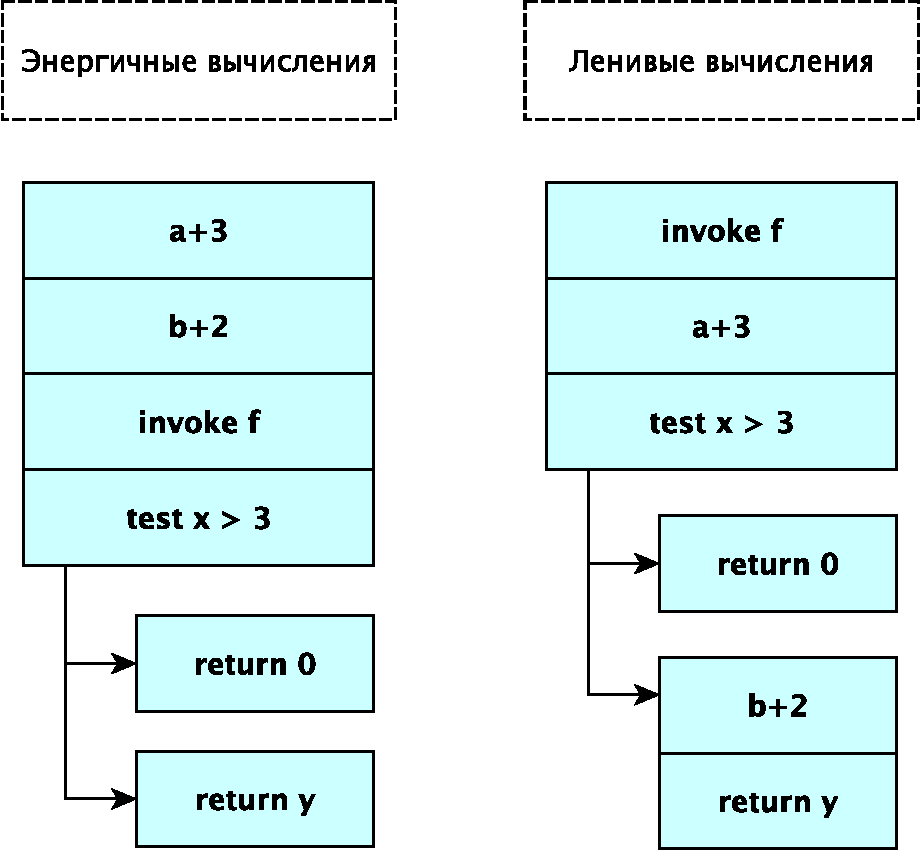
\includegraphics[width=0.6\textwidth]{illustrations/lazyorder-crop.pdf}
\caption{Ленивые и энергичные вычисления}
\label{fig:lazy_calc}
\end{figure}

Видно, что при ленивых вычислениях, реальное вычисление результата выражения откладывается насколько это возможно. Это создает свои проблемы: скажем передавать в функцию такое недосчитанное выражение гораздо сложнее, чем передать посчитанное заранее число. Поэтому ленивые вычисления в C++ встречаются только в нескольких контекстах:

\begin{enumerate}
\item В вычислениях с длинными логическими операциями: \lstinline!&&! и \lstinline!||!. Из-за ленивого порядка их применения, легальны выражения вида:
\begin{lstlisting}
if (p && p->next) { /* ... */ }
\end{lstlisting}
Если бы порядок вычисления был энергичным, то при нулевом указателе второе условие взорвалось.
\item В инстанцировании шаблонов
\item В исполнении константно-выраженных (constexpr) функций
\end{enumerate}

Итак шаблонное инстанцирование обязано работать лениво. Это означает, что проверены на корректность будут только те части шаблона, которые действительно были использованы в коде.

Пример вроде бы нарушает стандарт

\begin{lstlisting}
template <int N>
struct Danger {
  typedef char block[N]; 
};

template <typename T, int N>
struct Tricky {
  void test_lazyness() {
      Danger<N> no_boom_yet;
  }
};

int main() {
  Tricky<int, -2> ok;
}
\end{lstlisting}

Несмотря на то, что инстанцирование определяет \lstinline!typedef! с некорректным параметром размера массива, это не является ошибкой, поскольку реально этот зависимый тип нигде не был использован. Ленивость вынуждает компилятор откладывать инстанцирование любой части шаблона так долго, как это возможно.

\pagebreak
\subsection{Идиома SFINAE}\label{SFINAE}

\hfill\textit{I can accept failure, everyone fails at something.}

\hfill\textit{But I can't accept not trying.}{\vspace{0.5em}}

\hfill\textit{-- Michael Jordan}

Одной из важнейших идиом в правилах инстанцирования является SFINAE, что означает \textbf{substitution failure is not an error}. Она означает, что неудача при подстановке шаблонных параметров сама по себе не является ошибкой.

То, что я перевожу как ``неудача'' подстановки (substitution failure) это на самом деле термин, означающий скорее невозможность, то есть в слове failure нет оттенка недетерминированности, который, увы, есть в слове неудача. При чтении это надо понимать. 

Формально SFINAE определяется так: если в результате подстановки в \textbf{непосредственном контексте} класса (функции, алиаса, переменной) возникает \textbf{невалидная конструкция}, эта подстановка неуспешна, но не ошибочна. Сочетание этих двух условий порождает \textbf{SFINAE-case}.

Неудачную подстановку можно продемонстировать на примере уже полюбившейся всем функции максимума:

\begin{lstlisting}
template <typename T> inline const T
max (const T a, const T b)
{
  return (a > b) ? a : b;
}
\end{lstlisting}

Семантически здесь указано, что оба аргумента имеют одинаковый тип. Таким образом, подстановка, в которой для них будут выведены разные типы, будет неудачной.

\begin{lstlisting}
int g = max (1, 1.0);
\end{lstlisting}

Что произойдёт? Благодаря принципу SFINAE, наткнувшись на неудачную подстановку, компилятор не будет паниковать и выдавать сообщения об ошибках. 

Возможно где-то определён более подходящий шаблон, например:

\begin{lstlisting}
template <typename T, typename U> inline const T 
max (const T a, const U b) { ... }
\end{lstlisting}

и подстановка в него завершится успехом.

Если нет, то сообщение об ошибке будет выглядеть довольно очевидно:

\begin{verbatim}
error: no matching function for call to ‘max(int, double)’
note: candidate is:
note: template<class T> const T max(T, T)
note: template argument deduction/substitution failed:
note: deduced conflicting types for parameter 
     ‘T’ (‘int’ and ‘double’)
\end{verbatim}

Ещё один пример неудачной подстановки -- порождение кода, не соответствующего типу данных. Например ниже у выведенного типа \lstinline!int*! явно нет зависимого подтипа \lstinline!ElementT!.

\begin{lstlisting}
template<typename T>
typename T::ElementT at (T const& a, int i) {
  return a[i];
}

int
f (int *p) {
  int x = at(p, 7); /* boom! */
  return x;
}
\end{lstlisting}

Но само по себе это тоже не ошибка. С другой стороны, здесь конечно сложно предложить как следует переписать код, чтобы специализировать функцию для правильной подстановки. 

Очевидный вариант:

\begin{lstlisting}
template<typename T, typename U>
U at (T const& a, int i) {
  return a[i];
}
\end{lstlisting}

Не работает, потому что компилятору неоткуда вывести тип \lstinline!U!.

Более интересный вариант использует новый стандарт и не требует наличия зависимых типов:

\begin{lstlisting}
template<typename T>
auto at (T const& a, int i) -> decltype(a[i]) {
  return a[i];
}
\end{lstlisting}

Здесь подстановка пройдет удачно. Интересно, что стандарт не допускает перегрузку функции по возвращаемому значению, но допускает перегрузку шаблонной функции по возвращаемому значению \textbf{и типу}.

Не любая ошибка инстанцирования это SFINAE-case. Подстановка должна быть в непосредственном контексте шаблонного объявления, это иногда нетривиально.

\begin{lstlisting}
int negate (int i) { return -i; }

template <typename T> T negate(const T& t) {
  typename T::value_type n = -t();
  // тут используем n
} 

negate(2.0); // ошибка
\end{lstlisting}

Здесь в контексте сигнатуры и шаблонных параметров нет никакой невалидности. Невалидность в теле не является SFINAE, это ошибка второй фазы трансляции.

Однако же, если переписать функцию \lstinline!negate! так, чтобы сделать из неё SFINAE-case, например введя неудачный подтип в возвращаемое значение, как показано ниже, тогда это будет ошибка подстановки и выберется перегрузка.

\begin{lstlisting}
template <typename T> T::value_type negate(const T& t) {
  typename T::value_type n = -t();
  // тут используем n
} 
\end{lstlisting}

Такие случаи нужно чувствовать и осознавать, что они могут втсречаться.

SFINAE является очень мощной техникой, позволяющей делать интересные вещи. Например определить на этапе компиляции имеет ли некий тип вложенный зависимый тип с определённым именем.

\begin{lstlisting}
template <typename T> struct has_typedef_foobar {
  typedef char yes[1];
  typedef char no[2];
 
  template <typename C>
  static yes& test(typename C::foobar*);
 
  template <typename>
  static no& test(...);
 
  static const bool value = 
     sizeof(test<T>(0)) == sizeof(yes);
};

struct foo {    
  typedef float foobar;
};

struct bar {    
};

int main() {
  cout << "foo: " << has_typedef_foobar<foo>::value
       << "\nbar: " << has_typedef_foobar<bar>::value
       << endl;
}
\end{lstlisting}

Этот код выведет результат \lstinline!foo: 1, bar: 0!, верно определив наличие зависимого типа \lstinline!foo::foobar! в \lstinline!foo! и его отсутствие в \lstinline!bar!. Эта техника может казаться с первого взгляда не очевидной. Я рекомендую изучить идею, пока она не станет ясна: понимание SFINAE это ключ к пониманию всего метапрограммирования.

\textbf{Домашняя наработка:} Попробуйте в таком же стиле проверить наличие метода \lstinline!foobar!, возвращающего обязательно \lstinline!float! и не берущего ни одного аргумента. Тривиальная замена:

\begin{lstlisting}
template <typename C> static auto test(void*) ->
      decltype(float {declval<C>().foobar()}, yes{});
\end{lstlisting}

До какой-то степени работает, но не ловит случаи когда возвращается \lstinline!float&! и т.п.

Всё это слишком запутывается. Я называю такое SFINAE ``партизанским'', потому что приходится блуждать в страшных зимних лесах без еды годами с оружием. Поэтому люди искали более систематические подходы.

И нашли их.

\pagebreak
\section{Систематическое SFINAE}

Проблемы с ``партизанским'' SFINAE во многом были вызваны тем, что область его применения была очерчена недостаточно исчерпывающе. Ясно, что возможны какие-то трюки, но какие трюки возможны, а какие нет, и, что важнее \textbf{почему} они вообще возможны?

\subsection{Истина и ложь}

Ключевой шаг в систематизации SFINAE это понимание того, что в языке кроме ``пространства типов'' и ``пространства значений'' есть также ``пространство характеристик валидности'' или SFINAE-space и при любой работе в SFINAE-контекстах мы отображаем одно на другое.

Базовое отображение типов на значения и обратно даётся удобным классом (часть стандарта C++14) \lstinline!integral_constant!

\begin{lstlisting}
template <typename T, T v> 
struct integral_constant {
  static const T value = v;
  typedef T value_type;
  typedef integral_constant type;
  operator value_type() const { return value; } 
};
\end{lstlisting}

Функции, работающие в SFINAE контекстах, должны как-то сообщать ответы ``да'' и ``нет'' на вопросы ``является ли это тем-то и тем-то?'', скажем: ``является ли тип аргумента указателем на функцию-член класса X с такой-то сигнатурой?''. Чтобы закодировать ответы, можно использовать простейшие из таких констант: интегральные булевы константы.

\begin{lstlisting}
using true_type = integral_constant<bool, true>;
using false_type = integral_constant<bool, false>;
\end{lstlisting}

И они же позволяют отображение из type-space на sfinae-space

\begin{lstlisting}
template<typename T, typename U> 
struct is_same : false_type {};

template<typename T> 
struct is_same<T, T> : true_type {};
\end{lstlisting}

Теперь благодаря SFINAE, будет работать

\begin{lstlisting}
assert (is_same<int, int>::value && 
        !is_same<char, int>::value);
\end{lstlisting}
 
Пользоваться каждый раз \lstinline!xxx::value! не всегда удобно. Чуть более удобно -- сделать алиас в виде шаблонной переменной.

\begin{lstlisting}
template<typename T, typename U> 
bool is_same_v = is_same<T, U>::value;
\end{lstlisting}

Теперь будет работать как полная, так и сокращённая версия

\begin{lstlisting}
assert (is_same_v<int, int> && 
        !is_same_v<char, int>);
\end{lstlisting}

Интересно, что эта проверка делает фактически обратное отображение из SFINAE-space (валидности и невалидности) на значения.

\subsection{Определители и модификаторы\index{Type traits}}\label{TypeTraits}

Естественное применение SFINAE, как следует из прошлого примера это определители и модификаторы типов. Задача определителя -- сказать что-то о типе (есть ли в нём ссылки и указатели, константен ли он или волатилен и т.п.), задача модификатора -- сделать что-нибудь с типом (убрать ссылку, добавить указатель, сменить волатильность на константность)

Пример стандартного определителя: является ли тип ссылкой

\begin{lstlisting}
template <typename T> struct is_reference : false_type {};
template <typename T> struct is_reference<T&> : true_type {};
template <typename T> struct is_reference<T&&> : true_type {};
\end{lstlisting}

Пример стандартного модификатора: убираем ссылку с типа

\begin{lstlisting}
template <typename T> 
struct remove_reference { using type = T; };

template <typename T> 
struct remove_reference<T&> { using type = T; };

template <typename T> 
struct remove_reference<T&&> { using type = T; };
\end{lstlisting}

Для модификатора полезен алиас (см. \ref{FriendUsing})

\begin{lstlisting}
template <typename T> 
using remove_reference_t = typename remove_reference<T>::type;
\end{lstlisting}

Я называю такие конструкции ``триадами'' и очень часто имено в три строчки записывается SFINAE определитель или модификатор.

К счастью, некоторые конструкции являются очень простыми. Настолько простыми, что, казалось бы, не требуют даже триад. Например добавление обычной левой ссылки

\begin{lstlisting}
// this code is terribly wrong
template <typename T> struct add_lref { using type = T&; };
\end{lstlisting}

Ну что может пойти не так при добавлении левой ссылки?

Но увы. В таком виде добавление левой ссылки не будет работать для \lstinline!void!. Причина банальная -- \lstinline!void&! это некорректно. В некорректном случае, как уже было сказано выше, хорошая идея это оставить всё как есть. Можно пойти путём инкрементальных улучшений и предусмотреть случай для \lstinline!void!.

\begin{lstlisting}
template <typename T> struct add_lref { using type = T&; };
template <> struct add_lref<void> { using type = void; };

template <> 
struct add_lref<const void> { using type = const void; };

template <> 
struct add_lref<volatile void> { using type = const void; };

template <> 
struct add_lref<const volatile void> { 
  using type = const volatile void; 
};
\end{lstlisting}

Красота пропала, но проблема не в этом. Проблема в том, что, а почему мы вообще уверены, что только \lstinline!cv-void! так себя ведёт? Кажется, мысль тут изначально пошла по неверному пути. Верный путь лежит через SFINAE: необходимо выразить \textbf{идею} того, что либо мы добавляем ссылку если можем, либо оставляем всё как есть если не можем.

\begin{lstlisting}
template <typename T, typename Enable> 
struct ALRimpl { using type = T; }

template <typename T> 
struct ALRImpl <T, remove_reference_t<T&>> { 
  using type = T&; 
}

template <typename T> 
struct add_lref : ALRImpl <T, remove_reference_t<T>> {}
\end{lstlisting}

Эта изящная триада и многие другие приведена в частности в докладе Arthur O'Dwyer на CppCon 2017 (TODO: добавить в список литературы?)

Решение красиво, но тяжеловесно из-за того, что полагается на поведение \lstinline!remove_reference_t!.

Сделать его куда более прозрачным можно с помощью шаблона \lstinline!void_t! (стандартизирован в 2017 году).

\begin{lstlisting}
template <class ...> using void_t = void;
\end{lstlisting}

Это по сути отображение пачки типов на Enabled, если каждый из них Enabled. С использованием этого улучшения, искомый модификатор будет выражен куда яснее.

\begin{lstlisting}
template <typename T, typename Enable> 
struct ALRImpl { using type = T; }

template <typename T> 
struct ALRImpl <T, void_t<T&>> { using type = T&; }

template <typename T> 
struct add_lref : ALRImpl <T, void> {}
\end{lstlisting}
 
Здесь убрано всё лишнее и можно ли сделать лучше -- не очевидно.

Системный подход к SFINAE делает даже тяжеловесный определитель наличия зависимого типа с данным именем (\lstinline!has_typedef_foobar! из \ref{SFINAE}) весьма простым и понятным.

\begin{lstlisting}
template <typename, typename = void_t<>>
struct has_typedef_foobar : false_type {};

template <typename T> 
struct has_typedef_foobar <T, 
   void_t<typename T::foobar>> : true_type {};
\end{lstlisting}

Основные преимущества системного подхода: ясное и корректное выражение мысли в коде. Язык продолжает развитие в этом направлении. Например в C++17 приведённый выше код можно переписать ещё проще, используя появившийся там \lstinline!std::is_detected!

\begin{lstlisting}
template <typename T> 
using has_typedef_foobar_t = decltype(T::foobar);

cout << is_detected<has_typedef_foobar_t, foo>::value << endl;
\end{lstlisting}

Тем не менее, много до сих пор остаётся творческим процессом.

\subsection{Вариабельные шаблоны для списков типов}

Типичная задача на конструирование определителей типов: сконструировать \lstinline!and_t <T, U>!, который является \lstinline!true_type! только если и \lstinline!T! и \lstinline!U! являются \lstinline!true_type!, иначе является \lstinline!false_type!.

Решение к этому моменту должно быть уже почти очевидно:

\begin{lstlisting}
template <typename T, typename U> 
struct and_t : false_type {};

template <> 
struct and_t <true_type, true_type> : true_type {};
\end{lstlisting}

Но что если необходимо написать чуть более сложный определитель: вычислить коньюнкцию целого списка типов? Или, скажем, установить равенство данного элемента одному из списка?

Здесь на помощь приходят вариабельные шаблоны.

\begin{lstlisting}
template<typename T, typename... List>
struct is_one_of;

template<typename T>
struct is_one_of<T> : false_type {};

template<typename T, typename... Tail>
struct is_one_of<T, T, Tail...> : true_type {};
\end{lstlisting}

Самое сложное и изящное это рекурсивный вызов:

\begin{lstlisting}
template<typename T, typename Head, typename... Tail>
struct is_one_of<T, Head, Tail...> : 
       is_one_of<Head, Tail...> {};
\end{lstlisting}

Таким образом вариабельные шаблоны позволяют рекурсию по списку типов гораздо естественней, чем это позволяли делать обычные шаблоны. Большое количество кода в известной книге \cite{mcpp} теперь может быть переписано гораздо проще.

\textbf{Вопрос к студентам:} Дан template parameter pack \lstinline!...Ts!, где каждый тип может быть либо \lstinline!true_type! или \lstinline!false_type!. Как узнать, являются ли они все \lstinline!true_type!?

Очевиден простой рекурсивный ответ:

\begin{lstlisting}
template <typename ...Ts>
struct all_true;

template <typename H, typename ...Ts>
struct all_true<H, Ts...> : 
       and_t<is_same<true_type, H>, 
            all_true<Ts...>> {};

template <>
struct all_true<> : true_type {};
\end{lstlisting}

Можно ли сделать изящней, не инстанцируя $O(N)$ типов?

\ifanswers
Более просветляющий ответ использует кортежи:

\begin{lstlisting}
template <typename H, typename ...Ts>
struct all_true<H, Ts...> : 
       and_t<is_same<true_type, H>, 
             is_same<tuple<H,Ts...>,
                     tuple<Ts...,H>>> {};
\end{lstlisting}
\fi

Часть из использованных здесь определителей есть в стандарте, другие можно сконструировать по мере необходимости (хотя иногда это бывает нетривиально).

Можно запомнить (это примерно столь же полезная для запоминания информация как первый 21 знак числа пи), что все что угодно, что встречается в корректной программе на C++14 может быть отнесено к одному из 14 базовых классов traits и только к нему одному. 

\begin{lstlisting}
template <class T> struct is_void;
template <class T> struct is_null_pointer;
template <class T> struct is_integral;
template <class T> struct is_floating_point;
template <class T> struct is_array;
template <class T> struct is_pointer;
template <class T> struct is_lvalue_reference;
template <class T> struct is_rvalue_reference;
template <class T> struct is_member_object_pointer;
template <class T> struct is_member_function_pointer;
template <class T> struct is_enum;
template <class T> struct is_union;
template <class T> struct is_class;
template <class T> struct is_function;
\end{lstlisting}

И кстати 14 это первые две цифры номера стандарта. Совпадение? Не думаю.

\subsection{Статический ассерт}

Некоторые утверждения можно проверить на этапе компиляции. Конечно, на этапе исполнения их, обычно, тоже можно проверить.

\begin{lstlisting}
int foo () {
  assert (sizeof(int) == 4);
  // more code here
}
\end{lstlisting}

Допустимо, но выглядит странно. И потом: неужели это нужно делать в каждой функции?

Идея: написать в глобальной области видимости

\begin{lstlisting}
CT_ASSERT (sizeof(int) == 4);
\end{lstlisting}

Удивительно, но это возможно даже на C. Первое, что приходит на ум, это нечто вроде этого:

\begin{lstlisting}
#define CT_ASSERT(pred) switch(0){case 0:case pred:;}
\end{lstlisting}

Или вот этого:

\begin{lstlisting}
#define CT_ASSERT(pred) do {int arr[pred ? 1 : -1];} while(0);
\end{lstlisting}

Оба способа известны чуть ли не с восьмидесятых и оба в целом негодные, потому что не годятся для размещения вне функций.

Годный способ реализации на языке C чуть более сложен (пример взят с  \url{https://stackoverflow.com/questions/807244/c-compiler-asserts-how-to-implement})

\begin{lstlisting}
#define CT_ASSERT(predicate) \
  impl_CASSERT_LINE(predicate,__LINE__,__COUNTER__)
#define impl_PASTE(a,b) a##b
#define impl_CASSERT_LINE(predicate, line, cnt) \
  typedef char impl_PASTE( \
    assertion_failed_##cnt##_,line)[2*!!(predicate)-1];
\end{lstlisting}

Он построен на том же контроле массивов отрицательной длины, но благодаря использованию \lstinline!typedef! подходит для глобальных упоминаний. Но нельзя не заметить, что этот способ какой-то мрачный...

Андрей Александреску \cite{mcpp} в 2001 году предложил красивый и специфичный для C++ способ решения проблемы статического ассерта.

\begin{lstlisting}
template <bool cond> struct CT_ASSERT;
template <> struct CT_ASSERT<true> {};
\end{lstlisting}

Эти две строчки поражают воображение своей элегантностью. И в целом это работает, но тут есть проблемы с выдачей сообщения (большинство ошибок в шаблонах удивительно нечитаемы), писать в коде надо треугольные скобки, а не круглые и, главное, приходится придумывать имя для каждого ассерта.

\begin{lstlisting}
CT_ASSERT<sizeof(int) == 4> myassert1; 
\end{lstlisting}

Это неудобно, так что с 2011 года на уровне языка ввели синтаксический сахар.

\begin{itemize}
\item Для языка C: \lstinline!_Static_assert (cond, message)!
\item Для языка C++: \lstinline!static_assert (cond, message)!
\end{itemize}

Статические ассерты бесплатны и служат частью документации кода.

\begin{lstlisting}
#include "mylib.h"
static_assert (MyLib::Version > 2, "Old Mylib");
static_assert (sizeof(int) == 4, "Incompatible environment");
// ..... etc
\end{lstlisting}

Если что-то можно проверить статически, лучше проверить это статически.

Для нас интересно, что статический ассерт пришлось вводить на уровне языка именно потому что SFINAE-путь его организации, хоть и существовал, оказался неудобным.

Тем не менее, для многих других вещей этот путь не только удобный, а, пожалуй и единственный.

\subsection{Условный тип и условный Enable}

Рассмотренный ранее статический ассерт отображает выражения на валидность. Можно ли отображать типы в типы либо невалидные характеристики в зависимости от выражений? Оказывается, что да.

Сначала простое, управляемое выражением, отображение типов.

\begin{lstlisting}
template <bool C, typename T, typename F> 
struct conditional { using type = T; }

template <typename T, typename F> 
struct conditional<false, T, F> { using type = F; }

template <bool C, typename T, typename F> 
using conditional_t = typename conditional<C, T, F>::type;
\end{lstlisting}

Эта триада называется условным типом. Она отображает значение \lstinline!C! (от англ. condition) как \lstinline!{true,false} -> {T, F}!.

Теперь можно проделать интересную операцию: выкинуть из условного типа всё, касающееся \lstinline!F!. В этом случае получается отображение \lstinline!{true,false} -> {T, Disabled}!

\begin{lstlisting}
template <bool B, typename T = void> 
struct enable_if { using type = T; }

template <typename T = void> 
struct enable_if<false, T> { }

template <bool B, typename T = void> 
using enable_if_t = typename enable_if<B, T>::type;
\end{lstlisting}

Полученный паттерн -- один из самых известных и один из самых полезных изо всех. Главное в нём то, что он позволяет выкидывать (SFINAE-out) нежеланные инстанциации шаблонов.

\begin{lstlisting}
template <typename T, 
          typename = enable_if_t<(sizeof(T) > 4)>>
void foo (T x) { do something with x }

foo('c'); // FAIL
\end{lstlisting}

До некоторой степени, \lstinline!enable_if! штука коварная. Например, очевидная задача: написать в пару приведённой выше функции, функцию, которая работает для \lstinline!(sizeof(T) <= 4)! не так уж и просто.

Очевидная идея не работает.

\begin{lstlisting}
template <typename T, 
          typename = enable_if_t<(sizeof(T) > 4)>>
void foo (T x) { do something with x }

template <typename T, 
          typename = enable_if_t<(sizeof(T) <= 4)>>
void foo (T x) { do something with x }

foo('c'); // overload failure
\end{lstlisting}

Увы, до разрешения подстановки и вообще до SFINAE здесь не доходит. С точки зрения компилятора, написана одна и та же функция и выбрать перегрузку не представляется возможным.

Можно, конечно, выкрутиться с dummy аругментом

\begin{lstlisting}
template <typename T, 
          typename = enable_if_t<(sizeof(T) <= 4)>>
void foo (T x, int dummy = 0) { do something with x }
\end{lstlisting}

Это работает, но совсем непонятно откуда такая ассиметрия на ровном то месте.

Одна из возможных правильных идей: разруливать этот контекст не шаблонным параметром, а перегруженным типом возвращаемого значения.

\begin{lstlisting}
template <typename T>
enable_if_t<(sizeof(T) > 4)>, void> 
foo (T x) { do something with x }

template <typename T>
enable_if_t<(sizeof(T) <= 4)>, void> 
foo (T x) { do something with x }

foo('c'); // ok
\end{lstlisting}

Так всё работает.

\textbf{Вопрос к студентам:} Является ли хорошей идея пожертвовать типом аргумента?

\begin{lstlisting}
template <typename T> void 
foo (enable_if_t<(sizeof(T) > 4)>, T> x) { 
do something with x 
}
\end{lstlisting}

Это тоже работает, но сделали ли бы вы так?

\ifanswers
Правильный ответ: с моей точки зрения это крайне плохая идея, так как она убивает вывод типов.
\fi

Красивое и симметричное решение для этой задачи также поулчается если рулить указателями а не типами в качестве шаблонных параметров.

\begin{lstlisting}
template <typename T,
          enable_if_t <(sizeof(T) > 4)>* = nullptr>
void foo (T x) { cout << x << " gt 4 bytes" << endl; }

template <typename T,
          enable_if_t <(sizeof(T) <= 4)>* = nullptr>
void foo (T x) { cout << x << " le 4 bytes" << endl; }
\end{lstlisting}

Здесь работоспособность основана на том, что параметры-указатели входят в анализ типов отдельной строчкой.

Фантастический пример использования \lstinline!enable_if! для создания условного \lstinline!explicit! был рассмотрен Стефаном Лававеем в его докладе на CppCon 2016.

\pagebreak
\section{Метапрограммирование}\index{Metaprogramming}

\hfill\textit{To iterate is human, to recurse divine}{\vspace{0.5em}}

\hfill\textit{-- L. Peter Deutsch}

Шаблонное метапрограммирование было открыто в 1994-м году. Эрвин Анрух (Erwin Unruh) на заседании комитета по стандартизации сделал доклад, из которого следовало, что шаблоны могут быть использованы для вычисления на этапе компиляции и продемонстрировал генератор простых чисел, который на этапе компиляции выводил в виде сообщений об ошибках простые числа от 2 до заранее заданного настраиваемого предела. Но этот генератор довольно сложен. Кроме того, он представлял собой довольно неочевидный код.

\subsection{Простая рекурсия и арифметика}\label{SimpleRecursion}

Начать следует с очевидного: метапрограммирование это обобщение систематического SFINAE на целочисленные вычисления.

\begin{lstlisting}
template<size_t N>
struct fact : 
  integral_constant<size_t, 
                    N * fact<N - 1>{}> {}; 

template<> struct fact<0> : 
  integral_constant<size_t, 1> {};
\end{lstlisting}

Теперь в коде можно легко вычислить факториал пяти:

\begin{lstlisting}
cout << fact<5>{} << endl;
\end{lstlisting}

Это вычисление не займёт ни секунды машинного времени: ответ будет известен уже на этапе компиляции.

Посмотреть как разворачиваются вычисления можно в специальной утилите metashell.

\begin{verbatim}
$ metashell
> #include <metashell/scalar.hpp>
> #include "meta-fact.hpp"
> #msh mdb factorial<6>::value
Metaprogram started
(mdb) ft
factorial<6>::value
+ factorial<6> 
| + factorial<5> 
| | + factorial<4> 
| | | + factorial<3> 
| | | | + factorial<2> 
| | | | | + factorial<1> 
| | | | | | + factorial<0> 
| | | | | | ` factorial<0>::(anonymous) 
| | | | | ` factorial<1>::(anonymous) 
| | | | ` factorial<2>::(anonymous) 
| | | ` factorial<3>::(anonymous) 
| | ` factorial<4>::(anonymous) 
| ` factorial<5>::(anonymous) 
` factorial<6> 
(mdb) quit
> #msh quit
\end{verbatim}

Также легко организовать вычисление чисел Фибоначчи

\begin{lstlisting}
template<size_t N> struct fibonacci :
  integral_constant <size_t,
                     fibonacci<N-1>{} +
                     fibonacci<N-2>{}> {};

template<> struct fibonacci<1> : 
  integral_constant<size_t, 1> {};

template<> struct fibonacci<0> : 
  integral_constant<size_t,0> {};
\end{lstlisting}

Здесь двойная (древовидная) древовидная рекурсия уже может несколько смущать.

Не слишком ли много времени потратит на этот процесс компилятор?

\subsection{Две модели вычислений}\label{ComputationModels}

Вернёмся к факториалу. Человек с опытом на C написал бы простую функцию, вычисляющую факториал числа, в итеративном стиле:

\begin{lstlisting}
int
fact_0 (int x)
{
  int i, res = 1;
  for (i = 2; i <= x; ++i)
    res *= i;

  return res;
}
\end{lstlisting}

Здесь для того, чтобы вычислить факториал понадобились две ячейки памяти -- изменяемые переменные \lstinline!i! и \lstinline!res!. Математик Алан Тьюринг в 1936-м году опубликовал статью из которой следовало, что очень сложные вычислительные процессы можно произвести, имея в своем распоряжении:

\begin{itemize}
\item ветвления (скажем оператор \lstinline!if! или тернарный оператор)
\item переходы (хороший пример -- любой цикл или простое \lstinline!goto!)
\item последовательное линейное исполнение инструкций
\item достаточное количество изменяемой памяти
\end{itemize}

Факториал переписанный в более Тьюринг-стиле, но все ещё на C показывает некий минимализм выразительных средств:

\begin{lstlisting}
int memory[3];

/* memory[0] is input and result */
fact_0:
  memory[1] = 1;
  memory[2] = 1;
  label t, fin;
t:
  memory[1] += 1;
  memory[2] *= memory[1];
  if (memory[1] > memory[0]) 
    goto fin;
  goto t;
fin:
  memory[0] = memory[2];
\end{lstlisting}

Некоторое время спустя, Стивен Клини обнаружил, что очень сложные вычислительные процессы можно произвести, имея в своем распоряжении:

\begin{itemize}
\item ветвления (скажем оператор \lstinline!if! или тернарный оператор)
\item вызовы функций с передачей аргументов
\end{itemize}

В этом случае вообще не требуется изменяемых переменных.

И правда, факториал можно записать иначе:

\begin{lstlisting}
int
fact_1 (int x)
{
  if (x < 2)
    return x;
  else
    return x * fact_1 (x - 1);
}
\end{lstlisting}

Такие функции были им названы \textbf{частично-рекурсивными} функциями и было доказано, что аппарат частично-рекурсивных функций эквивалентен по вычислительной мощности машинам Тьюринга и лямбда-выражениям

Порождаемый таким образом рекурсивный процесс вычислительно не слишком эффективен, поскольку выражение \lstinline!x * fact_1 (x - 1)! не может быть вычислено до полного вычисления всех рекурсивных вызовов. Таким образом нет аккумулятора (вернее он неявно размазан по рекурсивной цепочке). Аккумулятор тоже можно сымитировать, изменив факториал:

\begin{lstlisting}
int
fact_2_1 (int x, int idx, int product)
{
  if (idx > x)
    return product;
  else
    return fact_2_1 (x, idx + 1, product * idx);
}

int
fact_2 (int x)
{
  return fact_2_1 (x, 1, 1);
}
\end{lstlisting}

Теперь в metashell картинка иная

\begin{verbatim}
Metaprogram started
(mdb) ft
factorial2<6>::value
+ factorial2<6> 
| ` fact_rec<6, 2, 1> 
|   ` fact_rec<6, 3, 2> 
|     ` fact_rec<6, 4, 6> 
|       ` fact_rec<6, 5, 24> 
|         ` fact_rec<6, 6, 120> 
` factorial2<6> 
\end{verbatim}

Интересно, что обычные программы на C++ больше похожи на подсахаренные машины Тьюринга (с поправкой на структурное программирование, взрослые циклы и вызовы функций). А вот метапрограммирование больше напоминает подход Клини.

Метапрограмма рекурсивного факториала несколько сложнее итеративной.

\begin{lstlisting}
template <size_t n, size_t idx, size_t product> 
struct fact_rec : 
  integral_constant<size_t, 
                    fact_rec <n, idx + 1, product * idx>{}> {};

template <size_t n, size_t product> 
struct fact_rec <n, n, product> : 
  integral_constant<size_t, 
                    product * n> {};

template <size_t n> 
struct factorial : 
  integral_constant<size_t, fact_rec <n, 1, 1>{}> {};
\end{lstlisting}

Но она же и более поучительна.

\textbf{Домашняя наработка:} сравните по скорости оба подхода на вашем компиляторе.

\subsection{Ветвления и пример квадратного корня}\label{TemplateIfElse}

Следующий пример куда более нетривиален: предлагается на этапе компиляции посчитать целочисленный квадратный корень.

Первый шаг для решения такой задачи: прикинуть код на обычном C++, но в функциональном стиле:

\begin{lstlisting}
int
isqrt (int N, int lo = 1, int hi = N)
{
  int mid = (lo + hi + 1) / 2;

  if (lo == hi)
    return lo;
  else
    {
      if (N < mid * mid)
        return isqrt (N, lo, mid - 1);
      else
        return isqrt (N, mid, hi);
    }
}
\end{lstlisting}

Теперь этот код практически один в один может быть переложен на метапрограмму. Поскольку шаблонное инстанцирование даёт один уровень сопоставления с шаблоном, можно убрать самый верхний условный оператор.

Тогда завершение рекурсии будет выглядеть тривиально как \lstinline{return lo} выше

\begin{lstlisting}
template <int N, int S> 
struct Sqrt <N, S, S, S> :
  integral_constant<int, S> {};
\end{lstlisting}

Но что использовать для ветвления в общем шаге? На выручку приходит уже рассмотренный выше \lstinline!conditional_t!.

\begin{lstlisting}
template <int N, int L = 1, int H = N, 
          int mid = (L + H + 1) / 2> 
struct Sqrt :
  integral_constant<int, 
    conditional_t<(N < mid * mid), 
                  Sqrt<N, L, mid - 1>, 
                  Sqrt<N, mid, H>> {}> {};
\end{lstlisting}

Использование всё так же тривиально

\begin{lstlisting}
cout << Sqrt<16>{} << endl;
\end{lstlisting}

Рассмотренные примеры показывают, что в метапрограммах можно делать ветвления и циклы (через рекурсию), хранить промежуточные данные и выполнять над ними основные арифметические операции. Всего этого достаточно для того, чтобы доказать Тьюринг-полноту шаблонов C++\index{Turing completeness of templates}.

\subsection{Простые числа}\label{TemplatePrimes}

Благодаря вложенным классам, можно устраивать некую модульность в вычислениях и даже писать нечто, похожее на ``метаподпрограммы''. Большой пример с простыми числами сильно отличается от базового кода Анруха (его всегда можно найти в интернетах), но он несколько полезней, так как результаты печатаются не в виде ошибок, а доступны для использования.

// TODO: переписать систематичней

\begin{lstlisting}
template <int i>
struct NthPrime
{
  template <int p>
  struct is_prime
  {
    template <int n>
    struct n_divisors
    {
      template <int N, int M>
      struct is_divisor
      {
        enum { val = is_divisor <N, M - 1>::val + ((N % M) == 0) };
      };

      template <int N>
      struct is_divisor <N, 1>
      {
        enum { val = 0 };
      };

      enum { val = is_divisor <n, n - 1>::val };
    };
    enum { val = (n_divisors <p>::val == 0) };
  };

  template <int n, int m>
  struct search_step
  {
    enum { val = search_step <n - (is_prime <m>::val), m + 1>::val };
  };

  template <int m>
  struct search_step <1, m>
  {
    enum { val = m - 1 };
  };

  enum { val = search_step <i, 3>::val };
};
\end{lstlisting}

Использование очевидно:

\begin{lstlisting}
int main(int argc, char* argv[])
{
  printf("Prime 6: %i\n", NthPrime<6>::val);
  return 0;
}
\end{lstlisting}

\textbf{Домашняя наработка:} коды Грея на шаблонах



\pagebreak
\section{Вычисления времени компиляции}

\hfill\textit{Once you're const, you are ensconced}{\vspace{0.5em}}

\hfill\textit{-- Susan Powell}

Вычисления времени компиляции до выхода стандарта C++11 велись исключительно с помощью особой шаблонной магии, рассмотренной выше. В новом стандарте появился способ сделать это по человечески. Новое ключевое слово constexpr контролирует время выполнения выражения. Это позволяет создавать настоящие константы и константные выражения, заниматься метапрограммированием и многое другое. Здесь будут систематично рассмотрены все перечисленные возможности.

\subsection{Ещё раз о константности}\label{Constexpr}

Уже рассматривавшийся выше модификатор const служит для того, чтобы объявить некие данные неизменяемыми. Но когда этим не изменяемым данным будет в первый раз присвоено их (в дальнейшем окончательное) значение? It depends.

\begin{lstlisting}
const int MAXSIZE = numeric_limits<int>::max();
int arr[MAXSIZE]; /* not legal in C++ */
\end{lstlisting}

В этом примере значение максимального возможного целого будет присвоено MAXSIZE только в динамике. В результате на этапе компиляции, размер arr всё ещё неизвестен и строго соответсвующие стандарту C++98 компиляторы обязаны выразить этим свое неудовольствие (такие массивы возможны в C и часто для C++ это включают как расширение).

Те же проблемы испытывают статические данные в классах и структурах:

\begin{lstlisting}
struct S {
  static const int sz;
};
const int page_sz = 4 * S::sz; // run-time
const int S::sz = 256; 
\end{lstlisting}

Это законная запись. Инициализатор статической константы, как и было рассмотрено ранее, должен появиться вне класса. Далее \lstinline!page_sz! будет инициализирвоана верным значением, но потребует инициализации времени выполнения. Как ни странно, но совсем немного отличающийся код уже пройдет инициадизацию на этапе компиляции:

\begin{lstlisting}
struct S {
  static const int sz = 256;
};
const int page_sz = 4 * S::sz; // compile-time
const int S::sz;
\end{lstlisting}

Это довольно грустно и требует от программиста помнить все тонкие правила константности, что, конечно, нереально. Именно этим и было мотивировано введение в стандарт С++11 ключевого слова, делающего известность на этапе компиляции явной.

Как вообще могла бы быть объявлена функция \lstinline!numeric_limits<int>::max()! в C++98? Например так:

\begin{lstlisting}
#define INT_MAX (2147483647)

template <>
struct numeric_limits<int> {
  static inline int max () { return INT_MAX; }
};
\end{lstlisting}

Эта функция -- прекрасный кандидат на формирование константного выражения. Она:
\begin{itemize}
\item не \lstinline!void!, то есть возвращает какое-то значение
\item состоит из одного \lstinline!return! -- то есть не заводит локальных переменных и не использует стек
\end{itemize}

Именно в таких двух условиях, функция в C++11 может быть сделана \textbf{константно-выраженной} для чего используется ключевое слово \lstinline!constexpr!. Это ключевое слово отличает неизменность от неизменяемости.

\begin{lstlisting}
template <>
struct numeric_limits<int> {
  static constexpr int max () { return INT_MAX; }
};
\end{lstlisting}

Аналогично разворачивается пример со структурой: статическое константно-выраженное поле прекрасно работает.

\begin{lstlisting}
struct S { 
  static constexpr int sz = 256; 
};

constexpr int page_sz = 4 * S::sz;
constexpr int S::sz;
int arr[page_sz]; // ok
\end{lstlisting}

Но не каждый тип может быть так аннотирован. Уже для структуры S это не работает, \lstinline!constexpr S = {}! будет ошибкой. Всё дело в том, что константные выражения могут образовывать только \textbf{литеральные} типы.

Литеральным считается тип у которого есть литералы, такие как \lstinline!1!, \lstinline!1.0! или \lstinline!1ull!. Видно, что таких типов немного -- в основном это примитивные типы такие как \lstinline!int! и \lstinline!float!. Вы можете расширять их перечень, но об этом далее.

Для константных выражений действуют статические ассерты времени компиляции.

\begin{lstlisting}
constexpr int whole = 1; 
constexpr double half = 0.5;
static_assert (half < whole, "Hmm....");
\end{lstlisting}

Самые большие сомнения вызывают константно-выраженные значения с плавающей точкой. Это вызвано тем, что результат операций над ними на этапе исполнения может не совпадать с результатом операций на этапе компиляции:

\begin{lstlisting}
constexpr float ct = 1.0f / 3.0f;

void __attribute__ ((noinline))
magic_func (float x, float y)
{
  fesetround (FE_DOWNWARD);
  float rt = x / y;
  if (ct != rt) 
    cerr << "Failure: " << ct << " != " << rt << endl;  
}

magic_func (1.0, 3.0);
\end{lstlisting}

Здесь на экране будет показана просто шикарная ошибка: два визуально одинаковых числа оказываются неравны друг другу.

Константные выражения также имеют тёмные стороны для указателей и массивов. Например ниже приведена тривиальная, но не столь уж очевидная ошибка.

\begin{lstlisting}
constexpr int arr[] = {2, 3, 5, 7, 11};
constexpr int *x = &arr[3]; // FAIL
\end{lstlisting}

Здесь справа от равенства стоит \lstinline!const int*!, а слева стоит \lstinline!int* const!. Поэтому, чтобы всё работало правильно, нужно использовать несколько безумно выглядящую запись.

\begin{lstlisting}
constexpr const int *x = &arr[3]; // FAIL
\end{lstlisting}

Важно всегда отслеживать: константность \textbf{чего именно} в данном случае означает constexpr аннотация.

\subsection{Константно-выраженные функции}\label{Constexpr:functions}

Более интересный пример: что если сделать константно-выраженной обычную арифметичесмкую функцию?

\begin{lstlisting}
constexpr int square(int x) { return x * x; }
/* ... */
constexpr int res = square(5);
\end{lstlisting}

Здесь \lstinline!res! будет известен на этапе компиляции. Но при этом в таком виде:

\begin{lstlisting}
// foo's argument unknown at compile time
int foo (int y) { return square(y); }
\end{lstlisting}

Функция square (даже объявленная \lstinline!constexpr!) ведёт себя как самая обычная функция. Это позволяет иметь её одну, не заводя зоопарк \lstinline!constexpr! и не-\lstinline!constexpr! зверюшек.

В стандарте C++14 ослаблены ограничения на константно-выраженные функции. Начиная с этого стандарта, в такой функции могут содержаться:

\begin{itemize}
\item Все объявления, кроме \lstinline!static! и \lstinline!thread_local! переменных, а также неинициализированных переменных
\item Условные операции \lstinline!if! и \lstinline!switch!
\end{itemize}

Это делает написание таких функций гораздо более удобным. Например легальной становится следующая конструкция:

\begin{lstlisting}
constexpr int 
ipow (int x, int n) 
{ 
  int r = x;
  while (--n > 0) r *= x;
  return r;
}
\end{lstlisting}

Конечно это увеличивает работу для компилятора, но в сравнении с самой простой метапрограммой это выполняется куда быстрее и читается гораздо лучше.

Майерс в \cite{effmoderncpp} приводит блестящий пример совмещения вывода типов шаблонами с constexpr функциями: определитель размера массива.

\begin{lstlisting}
template <typename T, size_t N>
constexpr size_t arraySize (T(&)[N]) 
{
  return N;
}
\end{lstlisting}

Работает это например так:

\begin{lstlisting}
int keyVals[] = {2, 3, 5, 7, 11, 13};
int mapped[arraySize(keyvals)]; // same size
\end{lstlisting}

Здесь размер выводится из ссылки на массив аргумента.

\subsection{Аннотация данных}\label{Constexpr:data}

Чтобы отличать обычные данные от известных на этапе компиляции, данные и даже члены классов тоже можно аннотировать \lstinline!constexpr!

\begin{lstlisting}
struct S
{
private:
  static constexpr int sz; // constexpr variable
public:
  constexpr int two(); //constexpr function
};

constexpr int S::sz = 256;
enum DataPacket
{
  Small=S::two(), // error (call before def)  
  Big=1024
};

constexpr int S::two() { return sz*2; }
constexptr S s;

int arr[s.two()]; // ok (call after def)
\end{lstlisting}

Видно, что по существу они мало чем отличаются от обычных данных. Но компилятор имеет насчёт них точную гарантию что их значения при компиляции уже известны.

\subsection{Темные чудеса шаблонных переменных}\label{Constexpr:templatevars}

В отличии от C++11, в C++14 разрешено делать шаблонными не только классы и функции, но и переменные:

\begin{lstlisting}
template <typename T> T n = T(5);

int main() {
  n<int> = 10;
  cout << n<int> << " ";    // 10
  cout << n<double> << " "; // 5
}
\end{lstlisting}

Вместе с \lstinline!constexpr! аннотацией переменных, это позволяет вводить гораздо более симпатичные определители типов, рассмотренные в (\ref{TypeTraits}).

\begin{lstlisting}
template <typename T> 
constexpr bool is_void_v = is_void<T>::value;
\end{lstlisting}

Записывать \lstinline!is_void_v<T>! конечно гораздо проще и приятней, чем \lstinline!is_void<T>::value! (общий смех).

Но тогда возникает вопрос. Неужели у нас могут быть \lstinline!constexpr! данные типов \lstinline!int! или \lstinline!float!, но не может быть \lstinline!constexpr! данных пользовательских типов? Конечно могут.

\subsection{Аннотация конструкторов}\label{Constexpr:ctors}

Если у вас есть необходимость, чтобы ваш тип мог вести себя как compile-time константа, для него можно написать \lstinline!constexpr!-конструктор:

\begin{lstlisting}
struct Complex
{
  constexpr Complex(double r, double i) : 
    re(r), im(i) { }

  constexpr double real() const { return re;}
  constexpr double imag() const { return im;}
private:
 double re;
 double im;
};

constexpr complex c(0.0, 1.0);
\end{lstlisting}

Тело такого конструктора в C++11 обязано быть пустым, вся инициализация производится в списке инициализации. В C++14 это правило несколько ослаблено.

Для такого пользовательского класса можно ввести даже арифметику:

\begin{lstlisting}
struct Complex
{
  constexpr Complex(double r = 0.0, double i = 0.0) : 
    re(r), im(i) { }

  constexpr double real() const { return re;}
  constexpr double imag() const { return im;}

  constexpr Complex& operator+= (const Complex &rhs)
  {
    re += rhs.re;
    im += rhs.im;
    return *this;
  }

private:
  double re;
  double im;
};

constexpr Complex operator+ (const Complex &lhs, 
                             const Complex &rhs)
{
  Complex tmp = lhs;
  tmp += rhs;
  return tmp;
}
\end{lstlisting}

Но, конечно, всё это ООП времени компиляции является скорее изыском. Обычно такие абстракции в \lstinline!constexpr! не нужны и гораздо большее применение имеют пользовательские литералы.

\subsection{Пользовательские литералы}\label{Constexpr:userliterals}

Для определения пользовательского литерала, следует переопределить оператор кавычки.

\begin{lstlisting}
constexpr Complex operator "" _i( long double i )
{
  return Complex (0.0, i);
}
\end{lstlisting}

Теперь будет работать следующий код:

\begin{lstlisting}
  constexpr Complex c = 0.0 + 1.0_i;
\end{lstlisting}

Таким образом будет (на этапе компиляции!) создана константа пользовательского типа.

Строструп приводит даже более впечатляющий пример: \url{http://www.stroustrup.com/Software-for-infrastructure.pdf} (TODO: добавить в список литературы?)

\begin{lstlisting}
template<int M, int K, int S> struct Unit {
       enum { m=M, kg=K, s=S };
};

template<typename Unit> 
struct Value {
  double val; 
  explicit Value(double d) : val(d) {}
};
\end{lstlisting}

Далее ряд синонимов для тензорных индексов размерности:

\begin{lstlisting}
using Meter = Unit<1,0,0>;
using Second = Unit<0,0,1>;
using Second2 = Unit<0,0,2>; 
using Speed = Value<Unit<1,0,-1>>; 
using Acceleration = Value<Unit<1,0,-2>>;
\end{lstlisting}

И пользовательские литералы для удобного обозначения констант.

\begin{lstlisting}
constexpr Value<Meter> operator"" m(long double d)
{
  return Value<Meter> (d);
}   

constexpr Value<Second> operator"" s(long double d)
{
  return Value<Second> (d);  
}   

constexpr Value<Second2> operator"" s2(long double d)
{
  return Value<Second2> (d); 
}
\end{lstlisting}

Написав соответствующие перегрузки операторов деления, далее можно добиться статической проверки типов в удобной форме:

\begin{lstlisting}
Speed sp1 = 100_m/9.8_s;  // ok
Speed sp2 = 100_m/9.8_s2; // error (m/s2 is acceleration)
Speed sp3 = 100/9.8_s;    // error (100 has no unit)
Acceleration acc = sp1/0.5_s; // ok again
\end{lstlisting}

\textbf{Домашняя наработка:} добейтесь работы строчки \lstinline!constexpr Kilogramm mass = 5_kg + 3_lb!, где lb это фунты, на этапе компиляции строящей преобразование фунтов в килограммы.

\ifmoderncpp
\pagebreak
\section{Проектирование с учётом шаблонов}

\hfill\textit{All problems in computer science}

\hfill\textit{can be solved by another level of indirection}{\vspace{0.5em}}

\hfill\textit{-- David Wheeler}

Шаблоны, точно так же, как объектно-ориентированная подсистема не просто дают новые инструменты. Они существенно влияют на проектирование программ. В этом разделе будут рассмотены некоторые распространённые способы и приёмы проектирования с учётом шаблонов

\subsection{Характеристики}\label{sub:traits}

Определители и модификаторы типов из (\ref{TypeTraits}) представляют собой неплохую технику распознавания тривиальных свойств. Они позволяют ответить является ли тип указателем или можно ли сконструировать его объект по образцу. Но вообще=-то этого очевидно не достаточно.

TODO: traits here

\subsection{Классы политик}\label{subsub:policy}
\fi

\pagebreak
\section{Домашняя наработка по шаблонам}

\textbf{Контрольные вопросы}

\begin{enumerate}
\item Чем отличается вывод типов шаблонами от вывода типов через auto/decltype?
\item Какие сложности вносит в разрешение перегрузки тот факт, что функция может быть шаблонной?
\item Как заставить компилятор инстанцировать шаблон функции для конкретного типа только один раз на все единицы трансляции?
\item Не нарушит ли шаблон функции в заголовочном файле ODR при инстанцировании везде куда включен заголовочник?
\item Чем отличается статический полиморфизм от динамического полиморфизма?
\item Может ли программа на C++ быть быстрее, чем такая же программа на C, реализующая тот же алгоритм?
\item Может ли шаблонный класс иметь несколько перегруженных конструкторов копирования?
\item Чем отличается полная специализация от частичной?
\item Как вы будете выбирать между специализацией и перегрузкой шаблонных функций?
\item Может ли быть полностью специализирован метод внутри определения частично специализированного класса?
\item В C++ нет частичной специализации функций. Можно ли сымитировать её средствами языка?
\item Возможен ли вывод типа при конструировании экземпляра шаблонного класса?
\item На каком этапе разрешаются зависимые имена в шаблонах классов?
\item Как внутри шаблонного класса сделать имя метода, не зависящего от шаблонных параметров, зависимым? Зачем это может быть нужно?
\item Можно ли сконструировать объект шаблонного типа при наличии конкурирующей специализации этого типа?
\item Можно ли в зависимости от шаблонного параметра изменить тип единственного поля в классе без частичной специализации этого класса?
\item Может ли шаблонная функция быть виртуальной?
\item Как расшифровывается CRTP, зачем нужна эта идиома?
\item Как в C++ происходит разрешение грамматической неоднозначности при использовании шаблонов?
\item Может ли вариабельный шаблон быть частично специализирован по части пачки параметров?
\item Перечислите все значения троеточия (ellipsis) в грамматике языка.
\item Можно ли раскрытием пачки параметров сформировать поля в классе?
\item В каких случаях пустая пачка параметров делает шаблонный класс не шаблонным?
\item Какие методы для нерекурсивного доступа ко всем параметрам пачки вам известны?
\item Напишите безопасный относительно типов scanf или аргументируйте невозможность этого.
\item Можно ли найти номер поля в std::tuple по значению?
\item Напишите вариабельный шаблон функции, которая для своей пачки параметров возвращает второй с конца аргумент
%
% Лямбды
%
\item В каком случае вы предпочтете лямбда-функцию обычной? В каком наоборот?
\item Можно ли имея лямбда-функцию изменить что-то из захваченного ей по значению контекста и только потом вызвать её?
\item Можно ли захватить объект по правой ссылке (то есть по сути -- передать его в лямбда-функцию)?
\item Можно ли запретить для отдельной лямбда-функции move-семантику?
\item В лекциях описаны проблемы с наивным подходом к перегрузке лямбда-функций и их решение. Но почему не работает наивный метод?
\item Меняет ли захваченный контекст тип лямбда-выражения?
\item Может ли повиснуть (dangle) правая ссылка на захваченный контекст?
\item Может ли лямбда-функция принимать переменное количество аргументов?
\item Может ли обобщенная лямбда-функция быть специализирована? Частично специализирована?
\item В чём обобщённые лямбды уступают шаблонам функций и в чём превосходят их?
\item Можно ли ``перегрузить'' лямбда функции, заставив вызов \lstinline!foo(1)! против \lstinline!foo(1.0)! работать иначе, где \lstinline!foo! это лямбда и если да, то как?
\item Константно-выраженные лямбды в C++17: что это, зачем нужны, как работают.
\item Можно ли сымитировать захват по ссылке, располагая только захватом по значению с переименованием и если да, то как, а если нет, то чего не хватает?
\item Представим static переменную внутри лямбды. У объекта этой лямбды есть десять копий. Будет ли существовать девять статических переменных? Ответ обосновать.
\item Как написать рекурсивную лямбду и может ли она быть без захвата?
\item Иногда в коде перед лямбдами встречается значок плюса, например
\begin{lstlisting}
 +[](int x) { return x*2}
\end{lstlisting} 
Что это и зачем нужно?
\item Как бороться с возможным провисанием ссылок на захваченный контекст в крупных приложениях (где точно нереально просмотреть всё глазами)?
\item Что такое bind и какие его плюсы и минусы в сравнении с лямбдами?
%
% SFINAE
%
\item Как расшифровывается SFINAE, зачем нужна эта идиома?
\item Говорят, что подстановка шаблонных параметров работает лениво. Что это означает?
\item Чем может быть параметризован шаблонный класс?
\item Что такое метапрограммирование на шаблонах? Напишите мета-программу, вычисляющую числа Леонардо.
\item Напишите вычисление чисел Леонардо, используя integral constant.
\item Напишите вычисление чисел Леонардо как constexpr-функцию.
\item Представьте, что вы хотите иметь во время компиляции таблицу чисел Каталана. Как вы её себе организуете -- метапрограммой на шаблонах, препроцессором или constexpr-функцией? Аргументируйте свой выбор.
\item Для объявления нового типа вы можете использовать using или typedef. В каком случае что вы будете использовать?
\item Может ли constexpr-конструктор быть в чисто абстрактном классе?
\item В лекциях приведен пример статического контроля размерности. Напишите упомянутую там перегрузку оператора деления.
\end{enumerate}

\textbf{Задания}

\begin{enumerate}

\item
Реализовать поиск подпоследовательности в последовательности (алгоритм Кнута-Морриса-Прата) как обобщённую функцию

\item
В разделе (\ref{ConstVsDef}) был приведен совет (исходно принадлежащий Майерсу \cite{effcpp3d}) использовать где возможно \lstinline!const! вместо \lstinline!#define!. На это можно возразить, что, в случае отказа от препроцессора, простая проверка времени компиляции по значениям констант становится невозможной:

\begin{lstlisting}
#define T1 2
#define T2 3

/* compile-time check here */
#if T1!=T2
#error "T1 and T2 are inequal"
#endif
\end{lstlisting}

Можно ли реализовать такую же проверку, определив T1 и T2 как статические константы, а не как макроопределения?

\item 
Напишите реверсирующую прозрачную оболочку: функцию, которая вызывает переданную ей функцию с переданными ей аргументами в обратном порядке. Старайтесь минимизировать оверхед.

\item 
Напишите рандомизирующую прозрачную оболочку: функцию, которая вызывает переданную ей функцию с переданными ей аргументами в случайном порядке (предположите что типы всех аргументов совместимые). Старайтесь минимизировать оверхед.

\item 
Напишите код, который применяет к вариабельной пачке из k*N параметров для k=1,2,... произвольную функцию N аргументов и возвращает кортеж из k результатов.

\item 
Напишите безопасный относительно типов scanf на вариабельных шаблонах

\item 
Напишите SFINAE-определитель, отвечающий на вопрос, есть ли в классе перегруженный оператор сложения

\item 
Напишите SFINAE-определитель, добавляющий (если это возможно) правую ссылку к типу или оставляющий тип неизменным. Скажем \lstinline!int --> int&&!, но \lstinline!int[10] --> int[10]!

\item 
Напишите три функции вида \lstinline!int foo(T)!, параметризованные типом T, одна из которых инстанцируется только когда \lstinline!sizeof(T) <= 2!, вторая если \lstinline!2 < sizeof(T) <= 4! и третья если \lstinline!sizeof(T) > 4!. Все три должны существовать в коде одновременно, покрывая таким образом всё пространство вариантов.

\item 
Напишите на шаблонах метапрограмму, которая определяет старший значимый бит в числе на этапе компиляции.

\item 
Напишите на constexpr-функциях метапрограмму, которая определяет старший значимый бит в числе на этапе компиляции. Бонус за функцию, которая будет работать в C++11.

\item 
Спроектируйте простейшее compile-time отображение, параметризованное типами Key и Value.

\item 
Напишите constexpr функцию, берущую на вход \lstinline!std::tuple! и извлекающую его вторую треть.

\item 
Напишите выбрасывающую прозрачную лямбду: лямбда-функцию, которая вызывает переданную ей функцию, передавая ей каждый второй, переданный в лямбду параметр.

\end{enumerate}

\pagebreak
\chapter{Лабиринты стандартной библиотеки}\label{chap:stl}

\hfill\textit{Most software today is very much like an Egyptian pyramid}

\hfill\textit{with millions of bricks piled on top of each other,}

\hfill\textit{with no structural integrity,}

\hfill\textit{but just done by brute force and thousands of slaves}{\vspace{0.5em}}

\hfill\textit{-- Alan Kay}

Идея что включать и что не включать в стандартную библиотеку языка программирования не так тривиальна, как может показаться.

Некоторые языки поставляются с библиотеками включающими всё, что может понадобиться когда бы то ни было, включая крайне высокоуровневые функции работы с XML, базами данных, сетевыми протоколами. Это философия таких языков как Python, Java, C\#, которые идут ``с батарейками внутри''.

Стандартная библиотека языка С (и некоторых других) придерживается, наоборот, философии минимальной поддержки, включая только те функции, которые могут пригодиться каждому разработчику (и некоторые функции, которые вызвали слезы няшного умиления у комитета стандартизации и оставлены, хотя не нужны, пожалуй, вообще никому, например strcspn).

Язык C++ занимает промежуточную позицию. По своей задумке его библиотека придерживается второго подхода, но по факту от стандарта к стандарту асимптотически сходится к первому.

Стандартная библиотека языка C++ имеет долгую и интересную историю. 

Идея стандартизировать библиотеку в языке C (из которой позже выросла стандартная библиотека C++) возникла не сразу. Первая стандартизация библиотеки языка C это стандарт ANSI C 1989-го и последовавший за ним ISO/IEC 9899-1990 \cite{stdc90}. Эта библиотека известна под названиями libc или crt (от C run-time support) и в общем она довольно стабильна уже много лет и активно используется программистами. Но в этой библиотеке никогда не было ничего, похожего на контейнеры. Каждый раз, когда программисту на языке C нужен двусвязный список... ну что же, он пишет себе двусвязный список. В лучшем случае он где-нибудь находит готовый и молится, что найденное работает.

В самом начале пути языка C++, ещё на до-стандартном этапе, стало ясно, что возможности нового языка позволяют включить \textbf{обобщённые} контейнеры в том или ином виде. Первые шаги были сделаны когда в языке появились стандартные строки и потоки ввода-вывода.

Где-то к 1992 году, Алекс Степанов из Adobe, переписал с языка Ada на C++ свой проект, который он назвал STL -- стандартная библиотека шаблонов.

Этот проект был весьма странным для того времени: если язык C++ как таковой делался со строгим упором на ООП, Степанов разносил данные от методов их обработки, делал ортогональные итераторы и алгоритмы и в общем использовал скорее идеи функционального, чем объектно-ориентированного программирования. Тем не менее, результат получился превосходным и очень быстро, ещё до стандартизации в 98-м году библиотека STL стала индустриальным стандартом де-факто.

Одновременно с развитием контейнеров, пришло понимание роли исключений и важности написания кода с учётом исключений. К 2002-му году основные вопросы безопасности исключений в библиотеке были решены.

С тех пор развитие стандартной библиотеки не стоит на месте и в 2011 а потом и в 2017 она была несколько раз существенно расширена и переработана. Была добавлена даже поддержка работы с файловыми системами, обсуждается добавление средств работы с популярными сетевыми протоколами, были серьёзно пересмотрены аллокаторы.

В силу исторических особенностей своего формирования, стандартная библиотека языка C++ получала свои возможности слой за слоем. Сейчас это настоящий лабиринт, в котором, зная путь, можно сделать удивительные вещи удивительно просто.

В силу опыта чтения лекций, я считаю нужным начать не с контейнеров и не с итераторов, а с самой простой вещи, которая может быть на свете. Со строк. Тем более, они уже упоминались (см. \ref{subsubsec:cstrings})

\pagebreak
\section{Строки}\label{subsec:strings}

В самом общем виде, строка это массив символов с известной длиной. На самом деле, любой массив символов, известный на этапе компиляции, параметризован своей длиной как частью типа.

Например \lstinline?decltype("Hello, world!")? выведет \lstinline!const char (&) [14]!

\textbf{Вопрос к студентам:} а почему вывелась ссылка?

\ifanswers
Правильный ответ: массив это всегда lvalue, а для lvalue вывод decltype приписывает левую ссылку
\fi

Можно обратить внимание, что ``Hello, world!'' содержит тринадцать символов. Четырнадцатым является завершающий ноль, который неявно приписан в конец каждого строкового литерала.

Строка с завершающим нулём называется C-строкой (C-string). Вся унаследованная от языка С через хедер \lstinline!<cstring>! часть стандартной библиотеки C работает именно с C-строками.

Конечно, при работе со строками размер которых неизвестен на этапе компиляции, нужна некоторая унификация типов. Она достигается для C-строк через приведение их к указателю на первый элемент. Благодаря этому строки могут жить как в глобальной памяти, так и в куче или на стеке.

\begin{lstlisting}
const char *cinv = "Hello, world";
char cmut[] = "Hello, world";
char *cheap = malloc (/* some size */);
\end{lstlisting}

Здесь \lstinline!cinv! это указатель на первый элемент живущего в глобальной памяти строкового литерала (который поэтому является неизменным). При его инициализации копирования не происходит. С другой стороны, \lstinline!cmut! это строка на стеке или в изменяемой глобальной памяти. При её инициализации делается копирование строкового литерала в ячейки памяти и сама строка далее является изменяемой. Также изменяема и строка \lstinline!cheap!, но она уже явно выделена на куче под нужный размер.

Нет никаких проблем перебрасывать данные между разными типами памяти, скажем \lstinline!strcpy (cheap, cinv)! работает без проблем.

Две наиболее частые проблемы это утечка ресурсов при бездумном присвоении указателя и попытка присвоить указатель массиву (к счастью последнее это просто ошибка компиляции.

\begin{lstlisting}
cheap = cinv; // LEAK
cmut = cheap; // FAIL
\end{lstlisting}

Разумеется никто не запрещает взять \lstinline!char *pcmut = cmut! и далее \lstinline!pcmut = cheap! разумеется будет работать. Все технические проблемы здесь это обычные проблемы с массивами и указателями, они уже рассматривались ранее (см. \ref{subsec:arrpointers}).

\subsection{Проблемы безопасности в C-строках}\label{subsub:secproblems}

Когда при мне говорят, что в языке C строки представляют собой небольшую проблему в безопасности, я всегда выслушиваю это с тем же видом, с каким выслушал бы информацию о том, что тропический ливень, град и гроза представляют небольшую опасность намокнуть.

\begin{lstlisting}
void apply_world (char *sout, const char *sin) {
  strcpy(sout, sin);
  strcat(sout, ", world!");  
}
\end{lstlisting}

\textbf{Вопрос к студентам:} какие вы видите здесь проблемы с безопасностью? Ответ будет сразу ниже, не читайте его прежде чем сами не насчитаете хотя бы четыре пункта.

Коротко говоря, тут плохо всё. В первую очередь мы не можем быть уверены, что \lstinline!sout! указывает вообще на что-то разумное. Во-вторых даже если это так, не факт, что там достаточно памяти чтобы скопировать туда \lstinline!sin! и даже если достаточно, то в третьих не факт, что \lstinline!sin! указывал на нечто разумное и ограниченное по размеру. И даже, если указывал, то, в четвёртых, никто не знает сколько времени займёт копирование. И даже если немного, то, в пятых, неясно и нет возможности проверить хватит ли в \lstinline!sout! места на то, чтобы дописать туда ещё и кусок литерала.

Слишком много беспокойства о двух строчках кода, не так ли?

Пытаясь как-то учесть эти проблемы, люди сделали специальные функции с ограничением на размер буфера.

\begin{lstlisting}
char* strncpy (char *dst, const char *src, size_t n);
char* strncat (char *dst, const char *src, size_t n);
int strncmp (const char *s1, const char *s2, size_t n);
\end{lstlisting}

Но это слабое утешение.

Во-первых есть функции (скажем strlen) для которых так не сделать в принципе. А во вторых это всё равно не решает проблему подсовывания вместо осмысленного буфера чего угодно на вход функции.

Настоящая причина проблем – в том, что для C строки длина не является инвариантом. Чтобы сохранять инварианты таких объектов как строки, необходимо закрытое состояние, недоступное к модификации, т.е. необходима инкапсуляция. Что естественным образом приводит к идее: написать класс строки

\textbf{Вопрос к студентам:} вы хотели бы написать собственный класс строки с нуля?

Ответ на этот вопрос я предлагаю отложить до того момента, как мы познакомимся с тем как устроен класс строки в стандартной библиотеке.

То есть \lstinline!std::string!.

\subsection{Принципиальное устройство string}\label{subsub:strings}

Чтобы эффективно оперировать со строкой, нужно понимать её принципиальное устройство. Картинка (рис. \ref{fig:string-principal}) весьма условна и неполна, но она отражает тот взгляд, который может иметь достаточно прагматичный программист на строки в своей программе.

\begin{figure}[ht]
\centering
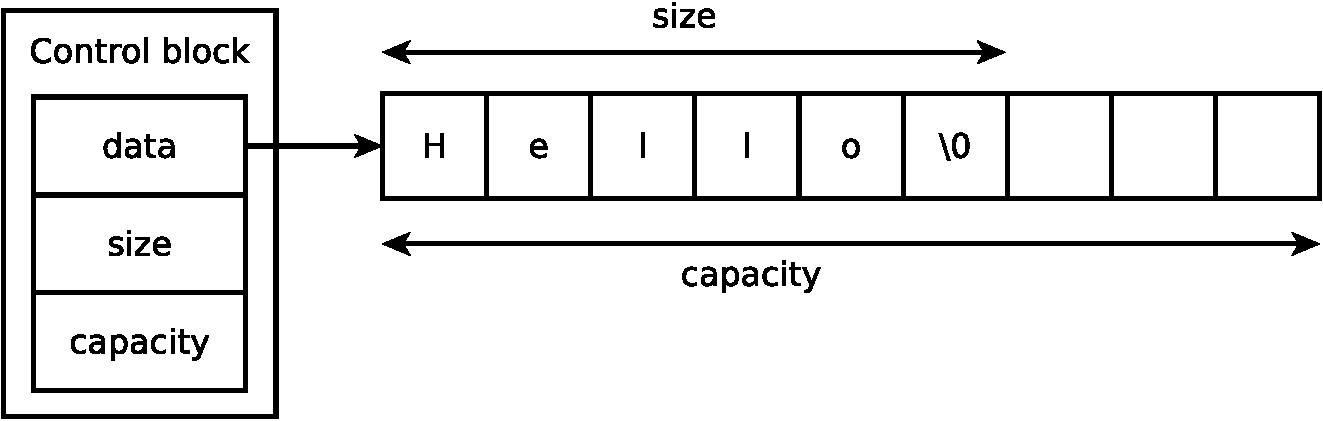
\includegraphics[width=1.0\textwidth]{illustrations/string-principal-crop.pdf}
\caption{Принципиальное устройство строки}
\label{fig:string-principal}
\end{figure}

Одна из странных вещей на этой картинке: здесь очевиден двойной контроль длины строки. Строка завершается нулём и, одновременно, её размер хранится как поле класса. Это сделано для эффективной работы метода \lstinline!c_str!, в частности, чтобы вообще иметь возможность сделать его \lstinline!const! методом.

Это в общем обычный класс, его методы всегда можно подсмотреть в документации. Для строк переопределены основные операторы (такие как сложение и сравнение на равенство), а также неизбежные копирование присваивание и перемещение.

В качестве чуть более интересного примера можно рассмотреть поиск в строке. Для этого есть сразу три метода:

\begin{itemize}
\item \lstinline!find! -- возвращает позицию подстроки в строке
\item \lstinline!find_first_of! -- возвращает позицию первого совпадения строки с одним из символов подстроки
\item \lstinline!find_first_not_of! -- возвращает позицию первого несовпадения с одним из символов подстроки
\end{itemize}

Метод \lstinline!find! возращает позицию как число, то есть номер символа в строке, являющегося началом найденной (в случае удачи) подстроки. При неудачном поиске возвращается специальное значение \lstinline!string::npos!. Важно помнить, что тип, в котором происходит поиск это обычно беззнаковый тип, так что \lstinline!npos! это чаще всего очень большое беззнаковое число. Поэтому важно не промахнуться с типом для его хранения. При поиске в строках следует всегда использовать \lstinline!string::size_type! иначе вы нарываетесь.

\begin{lstlisting}
string s = "Hello"; 
szt notfound = s.find("bye"); 
assert (notfound == string::npos); 
szt ellp = s.find("ell"); 
assert (ellp != string::npos); 
\end{lstlisting}

Иллюстрация работы этого кода приведена на (рис. \ref{fig:string-find}). 

\begin{figure}[ht]
\centering
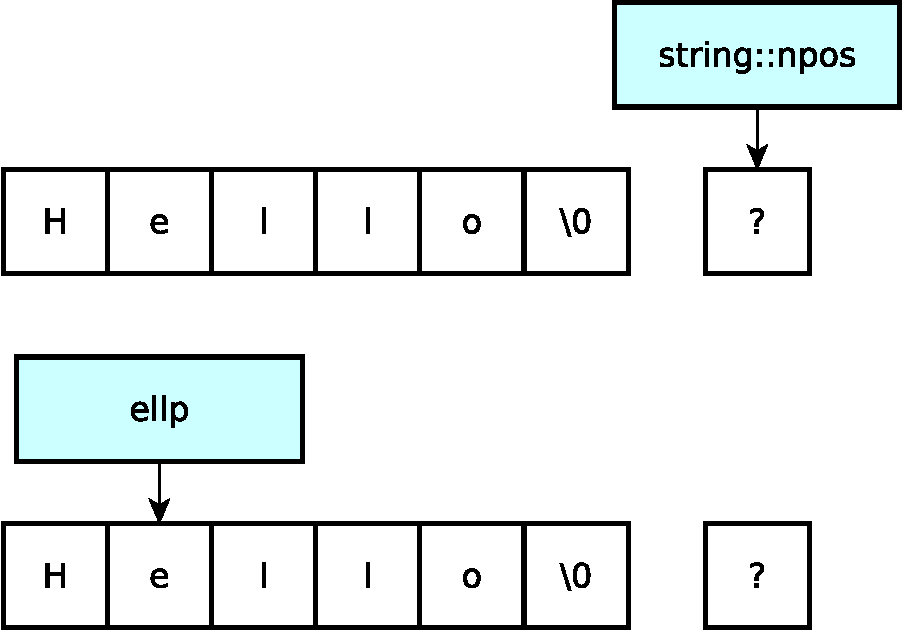
\includegraphics[width=0.6\textwidth]{illustrations/string-find-crop.pdf}
\caption{Поиск в строках}
\label{fig:string-find}
\end{figure}

Возможен также поиск с конкретной позиции

\begin{lstlisting}
szt hpos = s.find("H", ellp); 
assert (hpos == string::npos);
\end{lstlisting}

Разумеется начиная с позиции \lstinline!ellp! никакой буквы ``H'' в строке нет, поэтому она не найдена.

Простые задачи поиска просты и в C стиле. Например, приведённый выше код может быть переписан.

\begin{lstlisting}
const char s[] = "Hello";
char *notfound = strstr("bye", s);
assert (!notfound);
char *ellp = strstr("ell", s);
assert (ellp);
char *hpos = strstr(H", ellp);
assert(!hpos); 
\end{lstlisting}

Выгода начинает быть видна когда задачи становятся немного (немного!) менее тривиальными.

Каноническая задача -- заменить в строке все подстроки данного вида. Скажем в строке \lstinline!"Hello, $username, how are you doing, $username?"! заменить все вхождения \lstinline!$username! на \lstinline!Eric, the Bloody Axe!.

\textbf{Задача у доски:} написать это на C++ в стиле C без \lstinline!std::string!.

Задача непроста и требует некоторого размышления. Между тем на современном C++ она решается очень просто (даже не используя алгоритмов стандартной библиотеки, просто с помощью встроенных средств типа \lstinline!string!)

\begin{lstlisting}
void replace_all (string& str, const string& from, 
                              const string& to) 
{
  size_t ncur = 0;
  while ((ncur = str.find (from, ncur)) != string::npos) {
    str.replace (ncur, from.length(), to);
    ncur += to.length(); 
  }
}
\end{lstlisting}

В реальности эта функция будет чуть сложнее из-за контроля входных данных (например случая \lstinline!from.empty()!), но идея именно такая. Использовать её просто и приятно.

\begin{lstlisting}
string str = "Hello, $username, how are you doing, $username?";
string from = "$username";
string to = "Eric, the Bloody Axe";
replace_all (str, from, to);
cout << str << endl;
\end{lstlisting}

Конечно, вариант с C-строками можно написать так, что он выиграет у варианта с C++ строками представленного выше, но только на экстремально длинных строках, которые, в общем, редкость. Но да, в любом случае это надо учитывать. Автору приходилось убирать perf issues из кода, который занимался копированием сотен тысяч небольших строк через оператор присваивания класса \lstinline!string!. Об оптимизациях для небольших строк речь пойдёт позже. 

\subsection{Проблемы владения содержимым}\label{subsub:stringview}

Иногда в программе требуется константная статическая строка: нечто, что выделяется один раз и более не изменяется. В приступе эйфории от удобства строк, начинающий программист вполне может написать следующий код.

\begin{lstlisting}
static const string kName = "FOO";
// .....
int foo(const string &arg);
// .....
foo(kName);
\end{lstlisting}

\textbf{Вопрос к студентам:} чем он плох?

\ifanswers
Ответ ниже.
\fi

Вопрос в общем прост. Сложно догадаться задать его себе. Строка живёт в динамической памяти (т.н. ``куче''). Строковый литерал \lstinline!"FOO"! будет скопирован в свежевыделенное место кучи. После этого компилятор навсегда потеряет возможность статически доказывать нечто о его дальнейшей судьбе. Это называется heap indirection.

Допустим, проблема осознана и в качестве шага к её исправлению делается следующий: строка заменяется на указатель.

\begin{lstlisting}
static const char *kName = "FOO";
// .....
int foo(const string &arg);
// .....
foo(kName);
\end{lstlisting}

Это то, что китайские товарищи называют ``и было плохо а стало хуже некуда''. Теперь при вызове функции мы должны создать новый экземпляр временной строки, которая будет связана с константной ссылкой в формальном параметре.

\textbf{Вопрос к студентам:} как вы относитесь к идее существенно \textit{улучшить} ситуацию, заменив в сигнатуре функции ссылку на строку на указатель на C-строку?

\ifanswers
Правильный ответ: общий смех. Если найдётся несчастный, который согласится с тем, что это хорошая идея, его запинают его же одногруппники
\fi

Итак, кажется, достойного решения этой проблемы нет. Вернее не было. К настоящему времени проблема была осознана и в стандарт C++17 был добавлен вариант невладеющей строки \lstinline!string_view!. Его принципиальное устройство показано на (рис. \ref{fig:stringview-principal}).

\begin{figure}[ht]
\centering
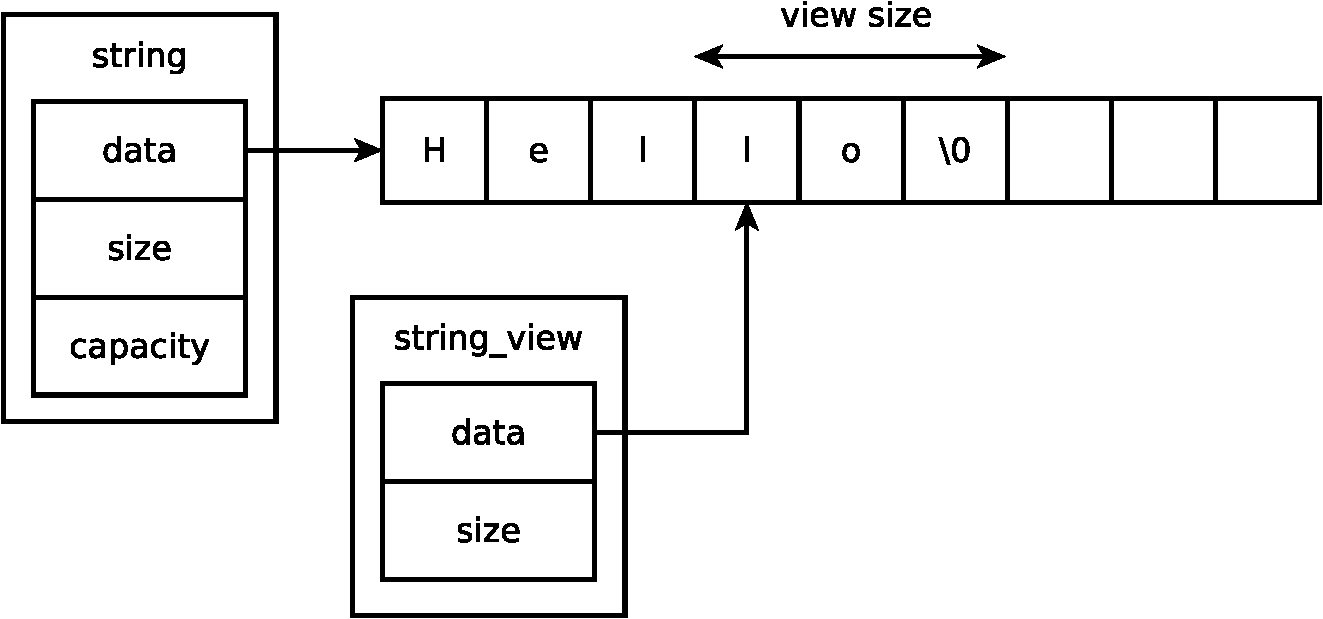
\includegraphics[width=1.0\textwidth]{illustrations/stringview-principal-crop.pdf}
\caption{Принципиальное устройство string view}
\label{fig:stringview-principal}
\end{figure}

С его помощью рассмотренная проблема решается просто, очень просто.

\begin{lstlisting}
static const string_view kName = "FOO";
// .....
int foo(const string_view &arg);
// .....
foo(kName);
\end{lstlisting}

В первой строчке нет heap indirection, поскольку \lstinline!string_view! не владеет своим содержимым и значит не должен иметь его локальную копию. По той же причине в последней строчке нет создания временного объекта, как и нет проблем с типизацией и безопасностью, присущих строкам в стиле C.

Базовые методы для \lstinline!string_view! это:

\begin{itemize}
\item \lstinline!remove_prefix! и \lstinline!remove_suffix! -- позволяют сдвинуть окно view слева и справа
\item \lstinline!copy! -- копирует подстроку в буфер (крайне опасный метод)
\item \lstinline!substr! -- возвращает view на подстроку
\item \lstinline!compare! -- около шести перегрузок этого метода делают различные сравнения
\item \lstinline!find! -- поиск по view
\item \lstinline!data! -- данные под view в сыром виде
\end{itemize}

Чтобы почувствовать как на самом деле выглядит работа с отображениями строк, полезно что-нибудь попробовать.

\begin{lstlisting}
string str = "   trim me  ";
string_view vtrim = str;
auto trimfst = vtrim.find_first_not_of(" ");
vtrim.remove_prefix(min(trimfst, vtrim.size()));
auto trimlst = vtrim.find_last_not_of(" ");
vtrim.remove_suffix(vtrim.size() - min(trimlst, vtrim.size()));
\end{lstlisting}

Отображения строк облегчают проблему владения, но не решают её. Следующий код мог бы написать человек с опытом Python.

\begin{lstlisting}
std::string a = ssl ? "https" : "http";
a = a + "://" + path + "/" + query;
\end{lstlisting}

Этот код вполне легален на C++ но давайте проследим как это будет работать.

Сначала будет создана строка \lstinline!a! и туда будет скопирован один из литералов. Далее будет создана временная строка из \lstinline!a + "://"! и в неё будет скопировано содержимое. Потом то же самое повторится ещё трижды. После этого результат будет скопирован в строку \lstinline!a!.

Это слишком много копирований. Хуже того: это слишком много реаллокаций памяти (а динамическую память дешево использовать, но довольно дорого выделять и освобождать). Гораздо лучше мы бы отнеслись к коду следующего вида:

\begin{lstlisting}
std::string a = 
  combine(ssl ? "https" : "http", "://", path, "/", query);
\end{lstlisting}

Но что это за функция \lstinline!combine!? В стандарте ничего такого нет. Самый простой вариант: сделать её строковым потоком. Но можно написать и настоящий комбинатор с использованием вариабельных шаблонов. При разговоре про потоки можно будет вернуться к тому как могла бы выглядеть такая функция (см. \ref{subsub:strstream}).

Ещё хуже тот факт, что часто нет возможности дать \textbf{гарантию}, что строка не владеет содержимым. Небольшая строка, допустим, уходит в какую-нибудь функцию. Она там может измениться, так что не может быть отображением, но чаще всего на практике она там не изменяется и таким образом владение было оплачено зря.

\begin{lstlisting}
void foo (string s);
string s1 = "Hello";
foo (s1);
string s2 = s1;
foo (s2);
\end{lstlisting}

Разумеется, такие случаи были замечены и активно обсуждались ещё с ранних 90-х. Одним из перспективных путей решения этого вопроса тогда казались строки с совместным использованием.

\subsection{Строки с совместным использованием}\label{subsub:cow}

В конце прошлого раздела была поставлена проблема совместного использования памяти строками. Основная идея здесь получила названием ``copy on write'' или сокращённо COW. Идея заключается в том, что строки совместно владеют одной и той же памятью пока они одинаковые и при этом достаточно умны, чтобы понять когда нужно перейти к единоличному владению если одной из них требуеся изменение (см. рис. \ref{fig:principal-cow})

\begin{figure}[ht]
\centering
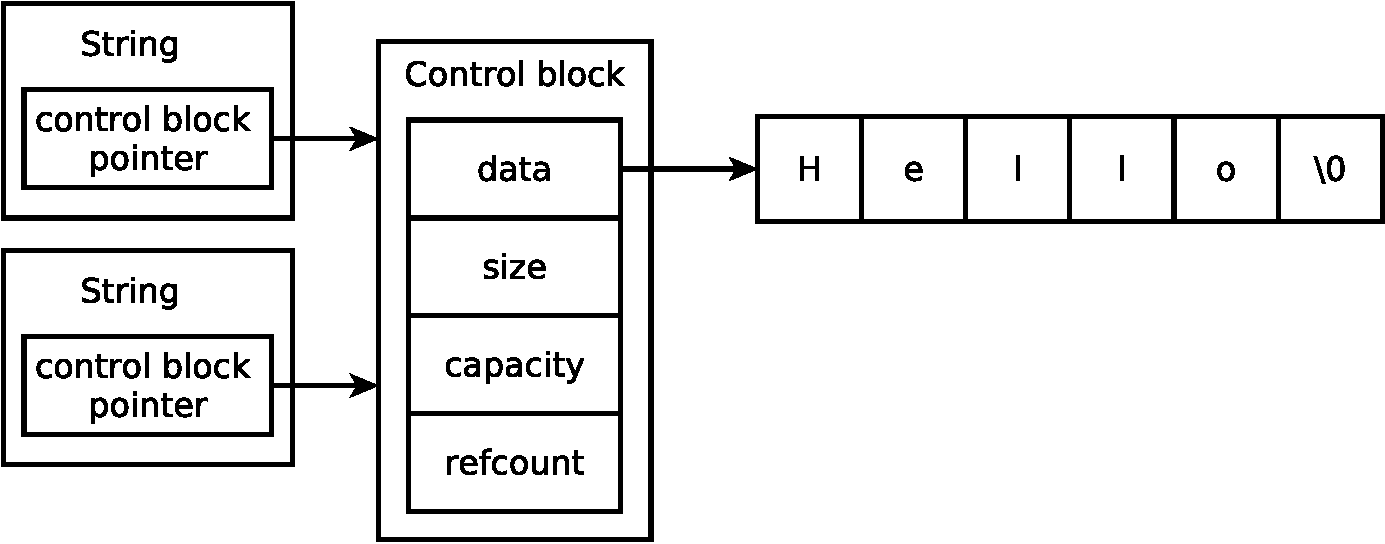
\includegraphics[width=1.0\textwidth]{illustrations/cow-principal-crop.pdf}
\caption{Идея copy on write строк}
\label{fig:principal-cow}
\end{figure}

Идея совместно используемых строк очевидно имеет свои плюсы и минусы.

К плюсам относятся:

\begin{itemize}
\item Экономия памяти
\item Дешёвое копирование (просто инкремент счётчика ссылок)
\item Меньше аллокаций и удалений в куче => прирост производительности
\end{itemize}

К минусам:

\begin{itemize}
\item Лишний уровень косвенности
\item Вирусное проникновение копирования во все модифицирующие операции
\item Проблемы thread safety (Multithread COW disease)
\end{itemize}

Эта идея была столь популярна, что была использована даже в GCC. Строка в GCC до версии 5 выглядела как показано на (рис. \ref{fig:string-cow-gcc}).

\begin{figure}[ht]
\centering
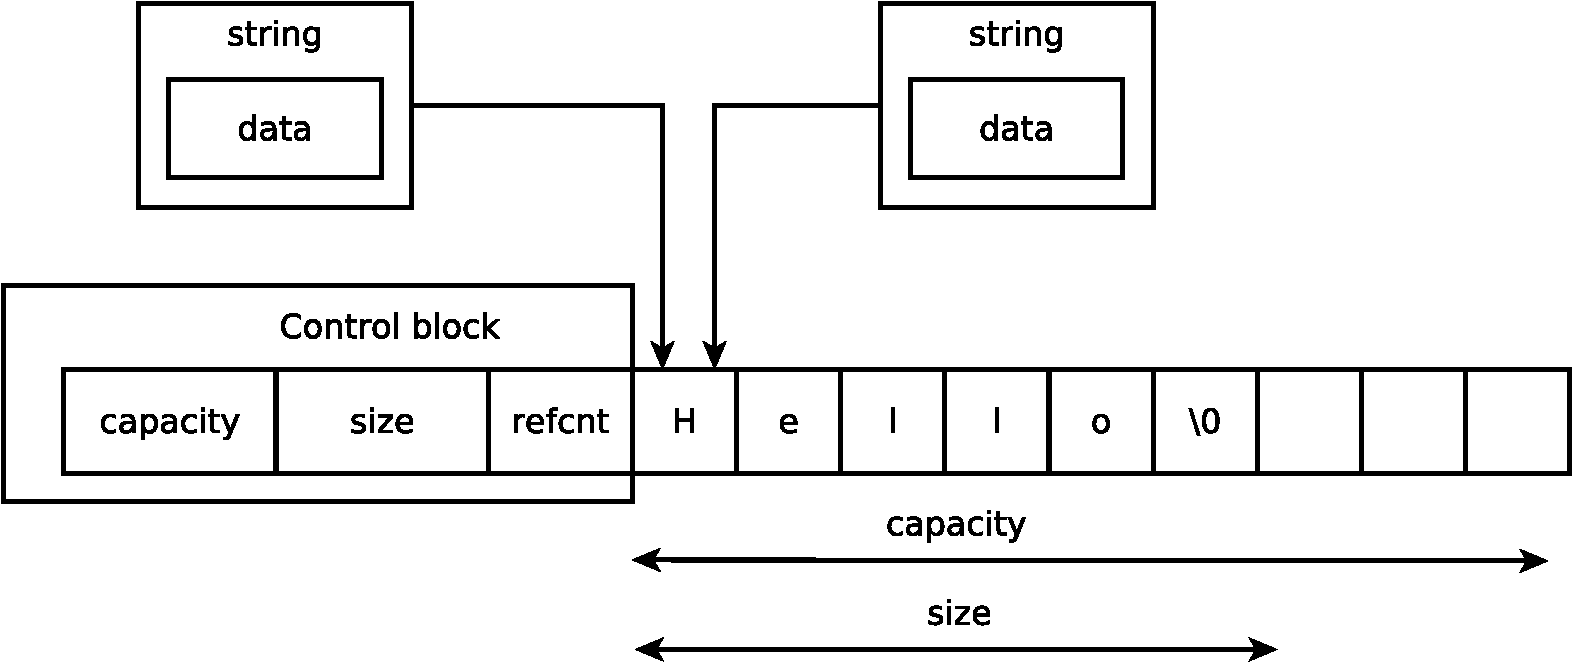
\includegraphics[width=1.0\textwidth]{illustrations/string-cow-gcc-crop.pdf}
\caption{Реализация copy on write строк в libstdc++ v5}
\label{fig:string-cow-gcc}
\end{figure}

Споры насчёт таких строк не утихали до тех пор, пока не был найден решающий аргумент: аргумент от \textbf{инвалидации} указателй. 

Дело в том, что при операциях над строкой некие указатели могут становиться недействительными.

\begin{lstlisting}
string s = "Hello";
const char *p = &s[3];
s += "world"; // p became invalid
\end{lstlisting}

В целом тут нет никаких проблем. Проблемы (проблемы!) начинаются когда совместно используемые строки (и только они) начинают инвалидировать указатели при операциях, в целом выглядящих крайне безобидно.

\begin{lstlisting}
string s = "Hello";
const char *p = &s[3];
s[0] = 'h'; // p valid for non-COW
            // p invalid for COW
\end{lstlisting}

В 2011 году официально было запрещено (TODO: stand link?) инвалидировать указатели при выполнении \lstinline!operator[]!, что исключает COW-реализации \lstinline!std::string!.

В итоге идиома COW находится в упадке: вне стандарта COW is almost dead.

\subsection{Оптимизации для небольших строк}\label{subsub:sso}

Ещё одной идеей как оптимизировать работу со строками являются оптимизации для небольших строк (SSO). Действительно, большинство строк в реальных программах невелики. Самый распространённый паттер это буквально пара слов текста на каком-нибудь человеческом языке. Идея в следующшем: если строка занимает меньше динамической памяти, чем поддерживающие структуры, может быть стоит и хранить её прямо на стеке в контрольном блоке? Идея проиллюстрирована на (рис. \ref{fig:string-sso-controlblock}).

\begin{figure}[ht]
\centering
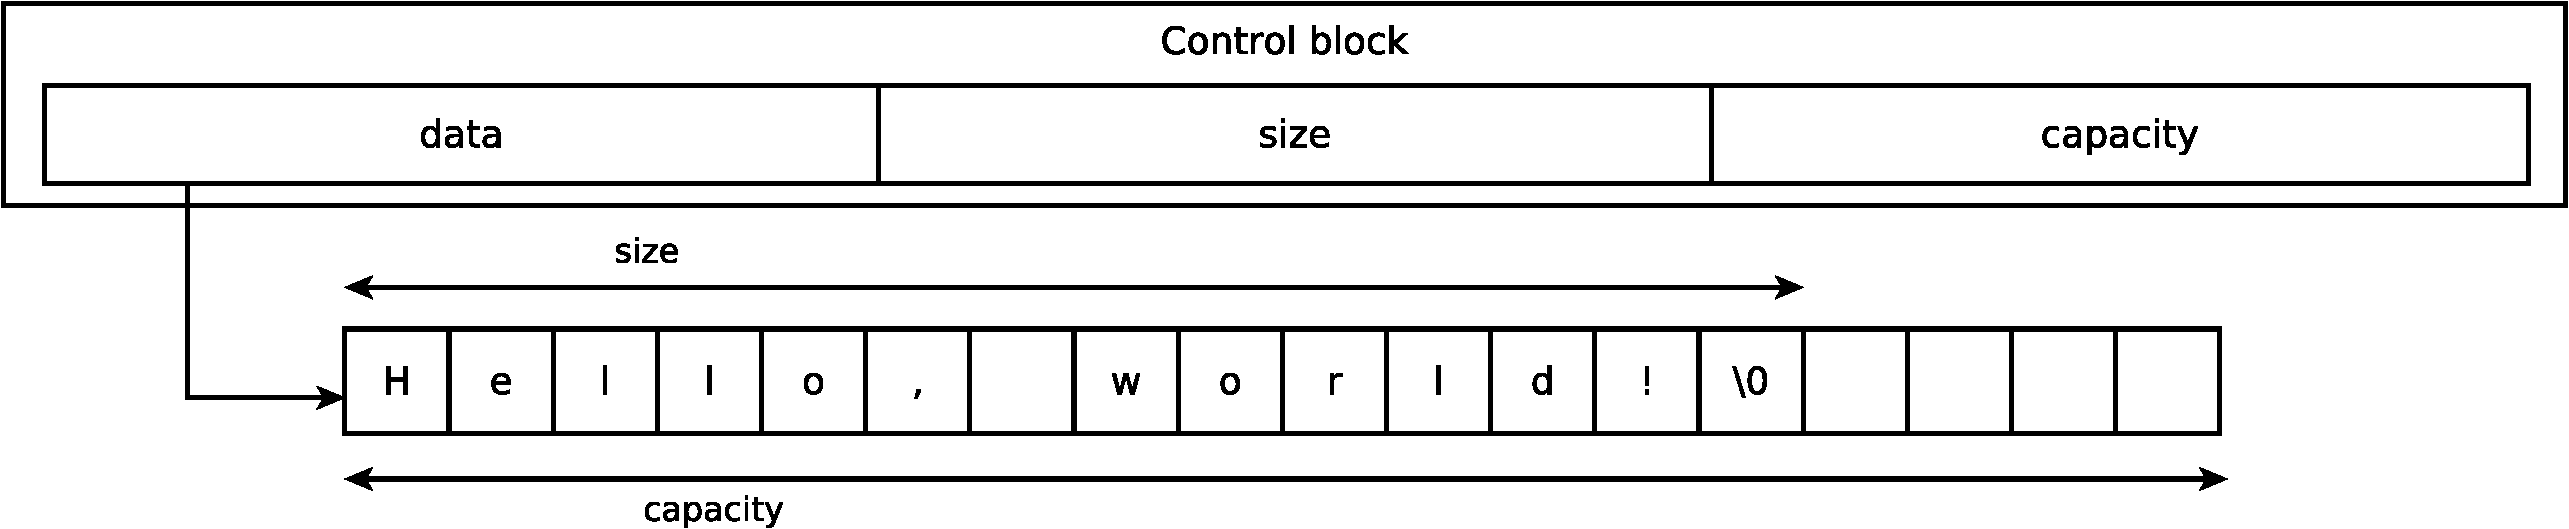
\includegraphics[width=1.0\textwidth]{illustrations/string-sso-controlblock-crop.pdf}
\caption{Идея для small string optimizations: настоящий масштаб для схемы строки}
\label{fig:string-sso-controlblock}
\end{figure}

Переводя это в код, можно написать нечто вроде:

\begin{lstlisting}
class string {
  size_type m_size;
  union {
    class {
      char *m_data;
      size_type m_capacity;
    } m_large;
    char m_small[sizeof(m_large)];
  };
// .....
};
\end{lstlisting}

В SSO можно увидеть и плюсы (они очевидны -- меньше реаллокаций и меньше места в куче) и минусы. Минусы это в первую очередь:

\begin{itemize}
\item Усложняется копирование и (что важнее) перемещение
\item  Добавляется время на выбор \lstinline!m_small! / \lstinline!m_large! при каждом доступе (в том числе чтении) с проверкой размера
\end{itemize}

Вторая проблема серьёзней. В GCC она решается так, как показано на (рис. \ref{fig:string-sso-gcc})

\begin{figure}[ht]
\centering
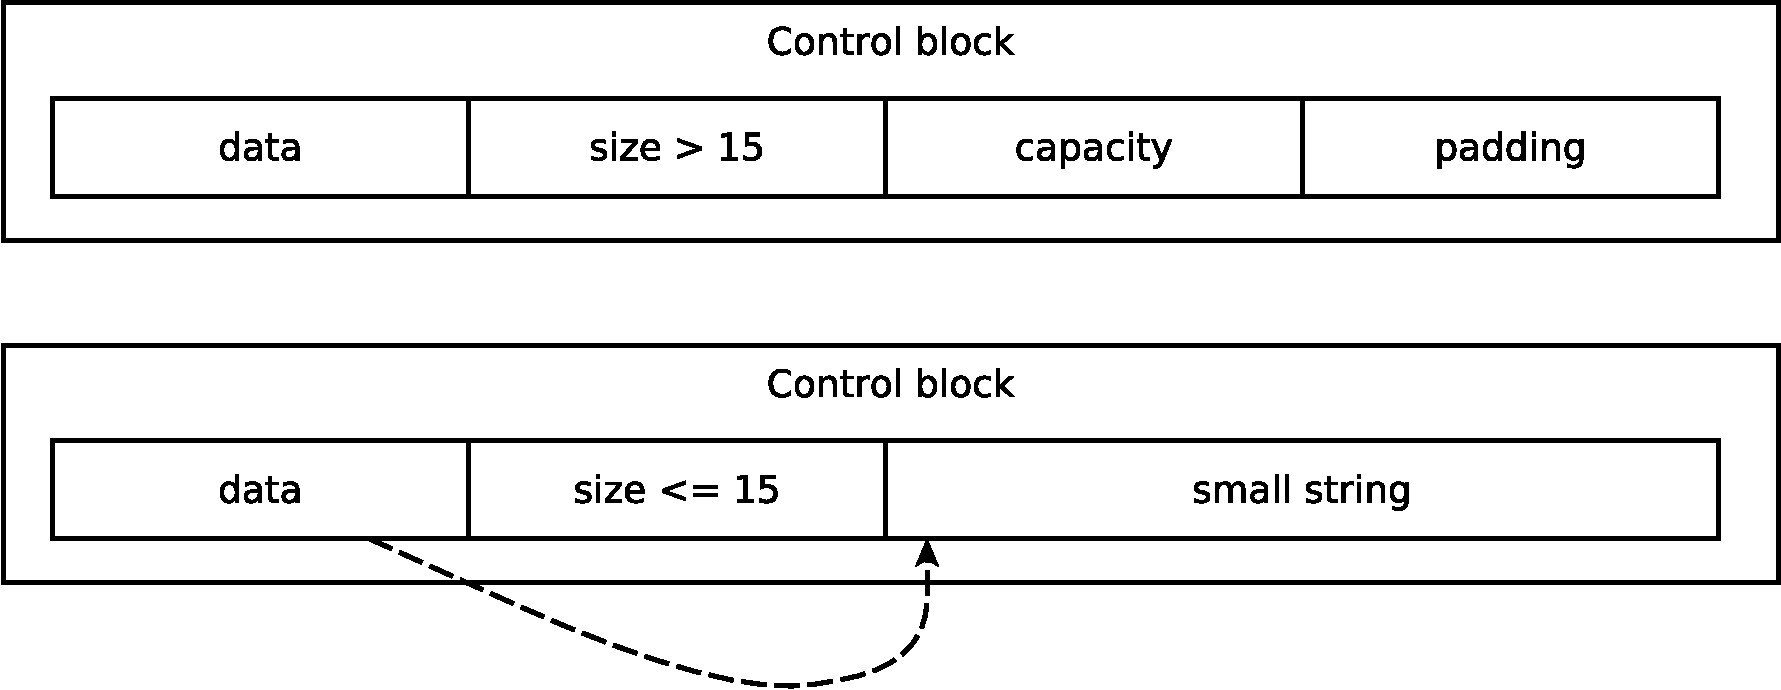
\includegraphics[width=1.0\textwidth]{illustrations/string-sso-gcc-crop.pdf}
\caption{SSO строка в libgcc версии выше пятой}
\label{fig:string-sso-gcc}
\end{figure}

Это решение позволяет избежать потерь времени при доступе, но уменьшает размер самой строки.

\subsection{Обобщения строк}\label{subsub:strtraits}

Пока что весь разговор вёлся в предположении, что строка это набор символов \lstinline!char!. Но вообще-то это не так. В некоторых кодировках символ занимает не один байт, а два (как в UCS-2) или четыре (как в UCS-4). Можно себе представить экзотические кодировки, где символ вообще будет иметь пользовательский тип или тип с плавающей точкой.

К счастью решение этой проблемы известно и это шаблоны. В первом приближении шаблон класса строки может выглядеть как-то так.

\begin{lstlisting}
template <typename CharT> class basic_string {
  CharT *data;
  size_t size;
  union {
    size_t capacity;
    enum {ALIGN = 32 - sizeof(data) - sizeof(size); }
    enum {SZ = (sizeof(capacity) + ALIGN - 1) / ALIGN;};
    enum {NUNITS = SZ / sizeof(CharT); }
    CharT small_str[NUNITS];
  } sso;
public:
  // all 89 methods goes here
};
\end{lstlisting}

Для удобства четыре его инстанциации могут быть определены через конкретные подстановки.

\begin{lstlisting}
typedef basic_string<char> string;
typedef basic_string<u16char_t> u16string;
typedef basic_string<u32char_t> u32string;
typedef basic_string<wchar_t> wstring;
\end{lstlisting}

Но это не отменяет необходимости реализовать все 89 методов, среди которых могут быть нетривиальные. Самые простые вопросы: как сравнивать символы, что такое завершающий символ, как копировать символы -- это вопросы, ответы накоторые сложно получить, не зная ничего о символе.

По традиции вся эта информация выносится в класс характеристик (traits\index{traits}). 

\ifmoderncpp
Техника характеристик типов уже была описана в (\ref{sub:traits}), это её применение.
\fi

\begin{lstlisting}
template <typename CharT> class char_traits;
\end{lstlisting}

Методы в этом классе: \lstinline!assign!, \lstinline!eq!, \lstinline!lt!, \lstinline!eof! и прочие, позволяют тонко настроить характеристики для конкретного типа символов.

Во втором приближении (с учётом характеристик), шаблон строки может быть переписан.

\begin{lstlisting}
template <typename CharT,
          typename Traits = std::char_traits<CharT>> 
class basic_string {
// all the same with traits
\end{lstlisting}

Но прежде чем можно будет умыть руки, нужно предусмотреть ещё одну деталь: выделение памяти на символ. Это явно не может быть свойством самого символа, потому что на одни и те же символы можно выделять память разными способами и с разными стратегиями. Но это не может быть также свойством строки по тем же причинам. Поэтому это обычно отделяется в специальный класс аллокатора.

\begin{lstlisting}
template <typename CharT,
          typename Traits = std::char_traits<CharT>
          typename Allocator = std::allocator<CharT>> 
class basic_string {
\end{lstlisting}

Об аллокаторах речь пойдёт далее (см. \ref{allocators}).

\textbf{Домашняя наработка:} пожалуй \textbf{теперь} вы знаете достаточно, чтобы построить свой велосипед строки. Сделайте это.

\pagebreak
\section{Исключения}\label{subsec:exceptions}

\hfill\textit{The most effective debugging tool is still careful thought,}

\hfill\textit{coupled with judiciously placed print statements.}{\vspace{0.5em}}

\hfill\textit{-- Brian W. Kernighan, 1979}

В предыдущем разделе ничего не было сказано про обработку ошибок при работе со строками и это не случайно. Строка это класс, а обработка ошибок при работе с классами требует нелокальных по природе механизмов, в частности исключений. Кое-что об исключениях уже было сказано ранее (см. \ref{subsec:basicexceptions}), но подробное изложение последует только в этом разделе, поскольку в стандартной библиотеке исключения использованы практически везде и настала пора понять зачем это нужно и как это работает.

Самым удивительным выводом этого раздела будет тот факт, что использование механизма исключений серьёзно влияет на проектирование кода: и на открытый интерфейс классов и на их внутреннее устройство. Хорошее понимание исключений открывает двери к пониманию многих проектных решений в стандартных контейнерах и в библиотеке вообще. Кроме того очень часто при поддержке унаследованного кода обнаруживаются скрытые ошибки, допущенные его менее опытными авторами именно в безопасности относительно исключений. Тем больше поводов внимательно разобраться в этом сложном и важном языковом механизме.

\subsection{Обработка ошибок в конструкторах}\label{subsub:ctorerrs}

Классическая обработка ошибок кодами возврата в стиле C ломается в C++ на специальных функциях, у которых непонятен контекст возврата. Самый простой пример это конструктор.

\begin{lstlisting}
template <typename T> class MyBuffer {
  T *arr_ = nullptr;
  size_t size_, used_;
public:
  MyBuffer (size_t sz): size_(sz), used_(0) {
    arr_ = (T*) malloc (sizeof(T) * sz);
    // here case of arr_ == nullptr shall be processed
  }
\end{lstlisting}

Как обработать ситуацию исчерпания памяти? 

Прежде чем отвечать на этот вопрос, можно подумать над другим вопросом: а собственно чем нам грозит эта ситуация, если её не обработать? Угроза на самом деле есть и она очень неприятная.

\begin{lstlisting}
MyBuffer b(100);
\end{lstlisting}

После этой строчки объект \lstinline!b! может оказаться в \textbf{несогласованном состоянии} (inconsistent state). У него будут выставлены поля \lstinline!v.arr_ = 0! т.к. память кончилась, но, при этом \lstinline!v.size_ = 100!, т.к. конструктор никак не обработал ошибку. 

Несогласованное состояние это бич объектно-ориентированных контекстов. Хуже всего то, что объект в несогласованном состоянии никак не отличается от нормального объекта: это даже не UB, такое состояние объекта вполне легально. Но инвариант класса нарушен и последствия от этого могут проявится через тысячи строк кода и тысячи часов исполнения.

Итак, обработка необходима, при этом вернуть код ошибки нет возможности. Можно поступить так, как поступают потоки ввода-вывода (см. \ref{subsec:iostreams}) и завести в классе особое поле state, устанавливая там какой-нибудь failbit или badbit. Но, конечно, это очень плохая тактика, потому что все такие механизмы разделяют ещё одну проблему с кодами ошибки: они \textbf{тихие}.

Объект, оказавшись в несогласованном состоянии должен информировать об этом создающий его контекст настолько громко, чтобы у контекста не было возможности проигнорировать эту информацию. В случае же кодов ошибок и, тем более, состояний потоков, более 90\% кода, который видел автор, просто игнорируют проверку.

На помощь приходят исключения.

\begin{lstlisting}
MyBuffer (size_t sz): size_(sz), used_(0) {
  arr_ = (T*) malloc (sizeof(T) * sz);
  if (!arr_) throw std::bad_alloc();
}
\end{lstlisting}

Здесь \lstinline!std::bad_alloc! это стандартный класс исключения. Этот код может быть даже упрощён, учитывая, что обычное поведение оператора \lstinline!new! это как раз сообщить исключением об исчерпании памяти

\begin{lstlisting}
MyBuffer (size_t sz): size_(sz), used_(0) {
  arr_ = new T[sz]; // throws bad_alloc
}
\end{lstlisting}

Человек, впервые оценивший всю мощь исключений, часто начинает лепить их по поводу и без повода. Важно отличать ошибки от исключительных ситуаций и правильно обрабатывать то и другое.

Исключительные ситуации характеризуются двумя важнейшими признаками:
\begin{itemize}
\item Состояние программы должно быть восстановимо
\item Исключительная ситуация не может быть обработана на том уровне, на котором возникла
\end{itemize}

Легко видеть, что в приведённом примере оба условия выполнены. Разумеется если нарушено первое условие, то лучшее, что можно сделать это завершить программу. Если же ошибка может быть обработана на том же уровне, она должна быть обработана, механизм исключений в этом случае является слишком дорогим и избыточным.

Всё дело в том, что порождение любого исключения инициирует размотку стека.

\subsection{Размотка стека}\label{subsub:unwinding}

Что выведет на экран исполнение следующего кода?

\begin{lstlisting}
struct UnwShow
{
  UnwShow () { printf ("ctor\n"); }
  ~UnwShow () { printf ("dtor\n"); }
};

void
foo (int n)
{
  UnwShow s;
  if (n == 0) throw 1;
  foo (n - 1);
}

/* ... */
foo (3);

\end{lstlisting}

Казалось бы здесь программа забирается глубоко в рекурсию и оттуда бросает исключение раньше чем какой-либо из созданных объектов выйдет из поля зрения. Тем не менее, на экране видны не только четыре конструктора, но и четыре деструктора! Что произошло? Произошедшее называется \textbf{stack unwinding} и по русски обозначается как \textbf{размотка} или \textbf{раскрутка} стека.

\begin{figure}[ht]
\centering
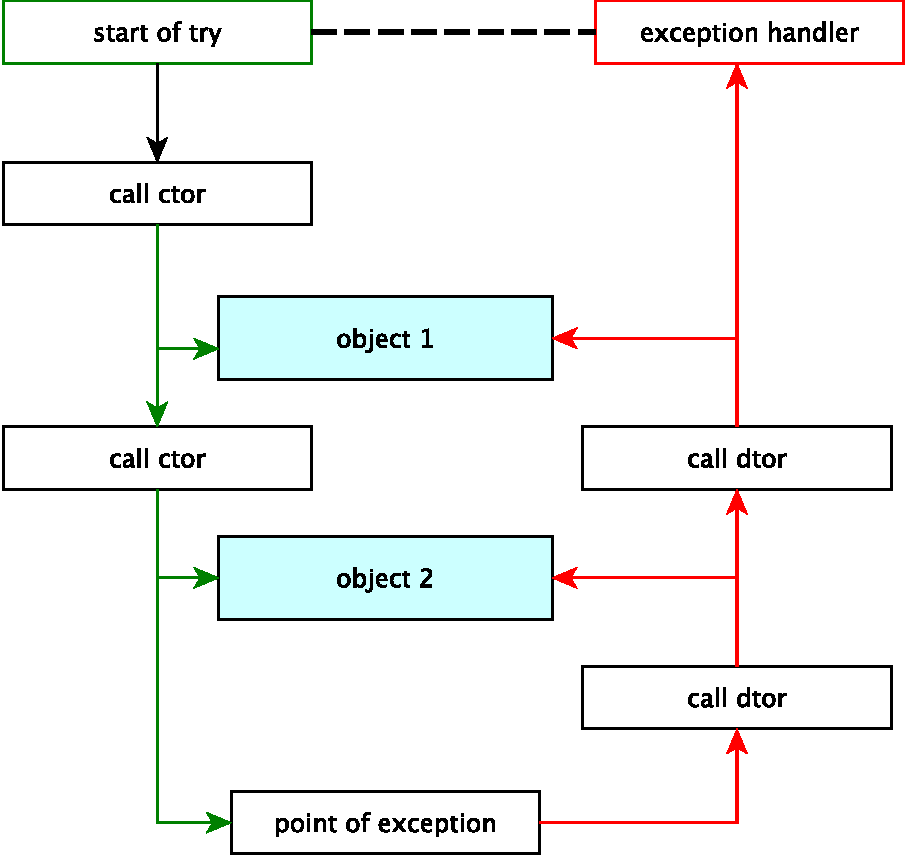
\includegraphics[width=1.0\textwidth]{illustrations/stack-unwind-crop.pdf}
\caption{Stack Unwinding}
\label{fig:stack_unwind}
\end{figure}

Процесс показан на (рис. \ref{fig:stack_unwind}). Довольно сложно показать на статичном рисунке динамический процесс раскрутки, но идея кажется ясной -- все объекты, созданные от места входа в обработку исключений (пока что можно считать что просто от начала программы) до обработчика удаляются со стека корректно -- то есть с вызовом деструкторов.

Раскрутка стека продолжается до тех пор, пока не будет найден первый подходящий \lstinline!catch!, которому и передаётся управление.

Ловля происходит по точному типу

\begin{lstlisting}
try { throw 1; } catch(long l) {} // NOT CATCH
\end{lstlisting}

Или по ссылке на точный тип

\begin{lstlisting}
try { throw 1; } catch(const int &ci) {} // CATCH
\end{lstlisting}

Или по указателю на точный тип

\begin{lstlisting}
try { throw new int(1); } catch(int *pi) {} // CATCH
\end{lstlisting}

Или по ссылке или указателю на базовый класс

\begin{lstlisting}
try { throw Derived(); } catch(Base &b) {} // CATCH
\end{lstlisting}

Catch-блоки пробуются в порядке перечисления

\begin{lstlisting}
try { throw 1; }
catch(long l) {} // NOT CATCH
catch(const int &ci) {} // CATCH
\end{lstlisting}

Пойманную переменную можно менять или удалять

\begin{lstlisting}
try { throw new Derived(); } catch(Base *b) { delete b; } // ok
\end{lstlisting}

Пойманное исключение можно перевыбросить

\begin{lstlisting}
try { throw Derived(); } catch(Base &b) { throw; } // ok
\end{lstlisting}

Ниже следует очень плохой пример, так не надо делать никогда:

\begin{lstlisting}
class MathErr {/* ... */};
class Overflow : public MathErr {/* ... */};

void foo()
{
  try {
    /* ... dangerous code here ... */
  }
  catch (MathErr) {
    /* ... dealing with other guys ... */
  }
  catch (Overflow) {
    /* ... dealing with overflow ... */
  }
}
\end{lstlisting}

В приведённом примере исключения перехватываются по значению. Это очень плохо и ведёт к проблеме срезки, рассмотренной в (\ref{Cutting}). Хорошо написанный код перехватывает исключения по константной ссылке или по указателю (если это конечно не исключения POD-типов, которые программист также имеет право возбуждать, их можно перехватывать по значению).

Важно понимать, что обработчики проверяются по порядку перечисления. Поэтому ставить обработчик \lstinline!MathErr! выше чем \lstinline!Overflow!, означает сделать последний чуть более чем бесполезным.

Итак правильный порядок: от частных к общим и ловить строго по косвенности

\begin{lstlisting}
catch (Overflow& o) { /* ... dealing with overflow ... */ }
catch (MathErr& e) { /* ... dealing with others ... */ }
\end{lstlisting}

\textbf{Вопрос к студентам:} как вы относитесь к ловле исключений по указателю?

\ifanswers
Правильный ответ: плохо. Возникают сложные проблемы владения выделенным объектом.
\fi

\subsection{Стандартные классы исключений}\label{subsub:stanclasses}

Хороший тон это генерировать потомка \lstinline!std::exception! или одного из его потомков в иерархии стандартной библиотеки.

\begin{figure}[ht]
\centering
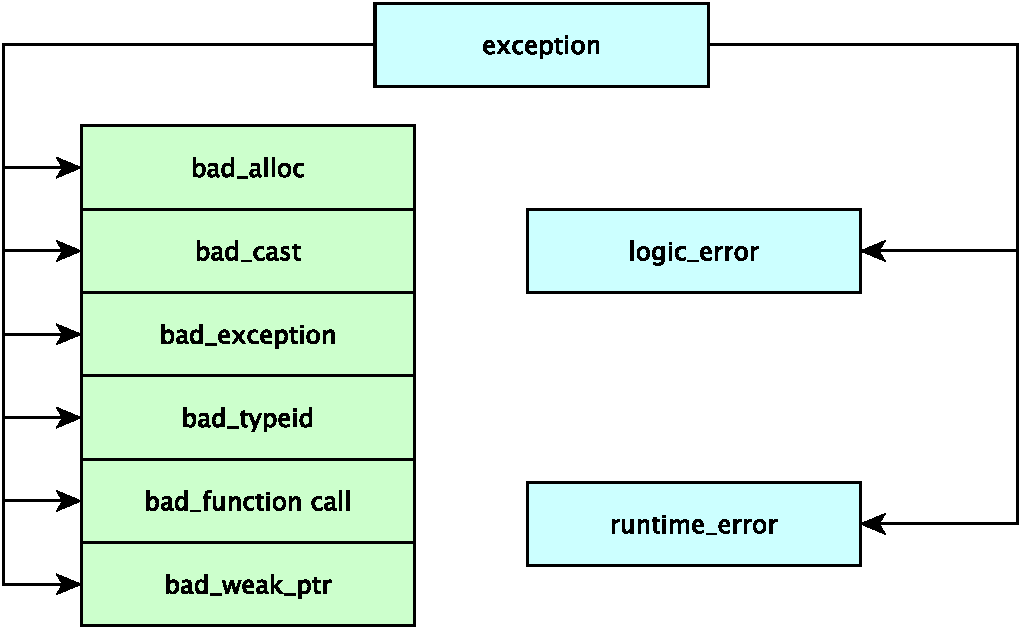
\includegraphics[width=1.0\textwidth]{illustrations/exc-hier-crop.pdf}
\caption{Иерархия стандартных исключений}
\label{fig:exc_hier}
\end{figure}

На (рис. \ref{fig:exc_hier}) слева зелеными обозначены те классы, которые могут быть выброшены в процессе работы со стандартной библиотекой. Справа -- два основных класса, от которых вам предлагается наследовать свои классы-обработчики.

\begin{lstlisting}
class MathErr : public runtime_error {/* ... */};
class Overflow : public MathErr {/* ... */};

void foo()
{
  try {
    /* ... dangerous code here ... */
  }
  catch (const Overflow &) {
    /* ... dealing with overflow ... */
  }
  catch (const MathErr &) {
    /* ... dealing with other guys ... */
  }
}
\end{lstlisting}

Такой вариант кода гораздо более правилен и плюс есть доступ к многочисленным полезным методам стандартных классов, которые они предоставляют. Самый простой пример это метод \lstinline!what()! у класса \lstinline!std::exception!, который возвращает строку с которой исключение было возбуждено

\begin{lstlisting}
throw runtime_error("Parameter value not allowed in context");

// a lot of code here

catch(exception const& e) { cout << e.what() << endl; }
\end{lstlisting}

При использовании стандартных классов рекомендуется быть осторожным с множественным наследованием

\begin{lstlisting}
struct my_exc1 : exception {
  char const* what() const;
};

struct my_exc2 : exception {
  сhar const* what() const;
};

struct your_exc3 : my_exc1, my_exc2 {};
\end{lstlisting}

Это конструкция опасна, потому что в итоге произойдёт нечто странное.

\begin{lstlisting}
throw your_exc3();

// a lot of code here

catch(exception const& e) { cout << e.what() << endl; }
catch(...) { cerr << "whoops!\n"; }
\end{lstlisting}

\textbf{Вопрос к студентам:} вы понимаете почему будет whoops?

\ifanswers
Правильный ответ: неоднозначный выбор из двух копий верхнего базового класса. Выход разумеется в виртуальном наследовании.
\fi

Как уже было сказано (см. \ref{subsub:exceptionguide}) у программиста есть соблазнительная возможность перехватить в своём обработчике не конкретные классы исключений, а вообще все исключения, используя для этого специальный синтаксис с троеточием. Здесь эта возможность была использована по делу, но вообще ей надо пользоваться с большой осторожностью, потому что в общем случае такой перехват может нарушить нейтральность функции относительно чужих исключений.

О нейтральности стоит поговорить отдельно.

\pagebreak
\subsection{Нейтральность}\label{subsub:neutrality}

Важным свойством исключительной ситуации является то, что она в принципе может быть обработана на каком-то уровне. Но чтобы быть обработанным, исключению нужно туда долететь.

\begin{figure}[ht]
\centering
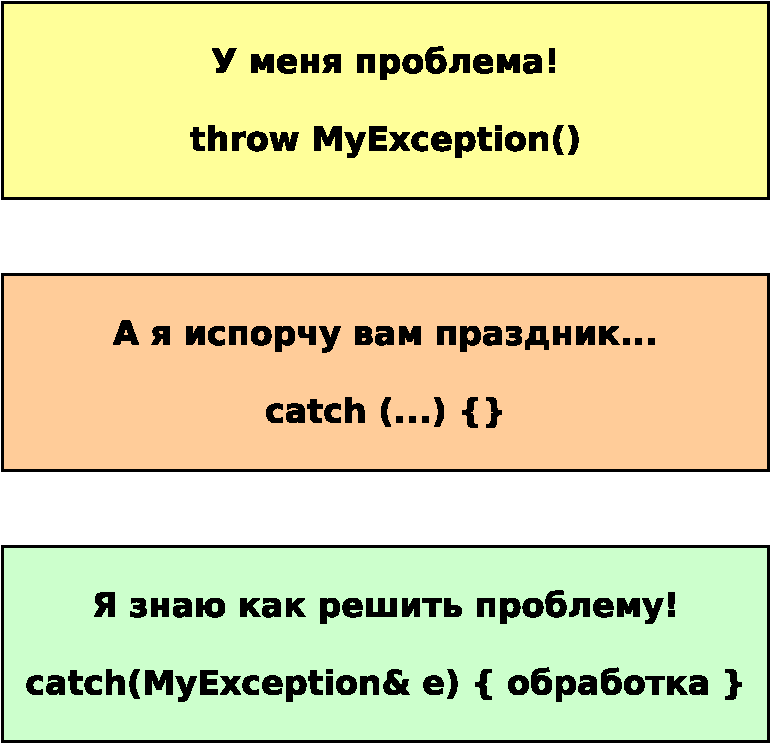
\includegraphics[width=0.6\textwidth]{illustrations/exc-neutrality-crop.pdf}
\caption{Нарушение нейтральности}
\label{fig:exc_neutral}
\end{figure}

На (рис. \ref{fig:exc_neutral}) показан случай, когда функция (обозначенная жёлтым) сообщает о проблеме, другая функция, обозначенная зелёным, может её обработать, но функция посередине просто ликвидирует нормальное движение объекта исключения вниз по стеку, перехватывая и свои и чужие исключения.

Такие функции называются нарушающими нейтральность.

Для сохранения нейтральности относительно исключений даже при необходимости поймать все исключения, пойманное исключение нужно дальше перевыбросить.

\begin{lstlisting}
int *critical = new int[10000]();
try {
  // a lot of dangerous code
}
catch (...) {
  delete [] critical;
  throw;
}
\end{lstlisting}

В этом фрагменте кода рассмотрен, пожалуй, единственный рациональный случай когда действительно нужно поймать все исключения и очистить критичный ресурс если что-то пошло не так.

\textbf{Вопрос к студентам:} а можно здесь вс-таки что-нибудь придумать чтобы обойтись без catch-all?

\ifanswers
Правильный ответ: да, например завернуть ресурс в RAII-обёртку, чтобы он был автоматически правильно очищен при размотке стека.
\fi

\pagebreak
\subsection{Гарантии безопасности}\label{sub:excsafety}

\hfill\textit{Exception handling isn't hard. Error handling is hard}{\vspace{0.5em}}

\hfill\textit{-- David Abrahams}

Исключения, являясь частным случаем нелокальной управляющей конструкции, добавляют строчки в неявный контракт на каждый метод и добавляют неожиданные дуги возможного выхода в каждом месте вызова небезопасной с точки зрения генерации исключений функции. Поэтому при проектировании кода, серьёзно использующего исключения, программист несёт дополнительную интеллектуальную нагрузку. Он должен следить за тем, что называется безопасностью кода относительно исключений.

Например для рассмотренного выше класса \lstinline!MyBuffer! очевидный конструктор копирования скорее всего будет в некотором смысле плох.

\begin{lstlisting}
template <typename T> class MyVector {
  T *arr_ = nullptr;
  size_t size_, used_;
public:
  MyVector (const MyVector &rhs) {
    arr_ = new T[rhs.size_]; // we will leak this memory
    size_ = rhs.size_; used_ = rhs.used_;
    for (size_t i = 0; i != rhs.size_; ++i)
      arr_[i] = rhs.arr_[i]; // if exception is thrown here
}
\end{lstlisting}

Этот пример был обнаружен Каргиллом в 1994 году \cite{Cargill} и подробно рассмотрен Абрамсом в 1998 \cite{Abrahams} и Саттером в 2000 и 2002 годах \cite{exceptionalcpp}, \cite{moreexceptionalcpp}.

Код, в котором при исключении могут утечь ресурсы, оказаться в несогласованном состоянии объекты и прочее, называется небезопасным относительно исключений. 

Существует три гарантии безопасности, которые может предоставлять код:

\begin{itemize}
\item
\textbf{Базовая гарантия} заключается в том, что сбой при выполнении операции может изменить состояние программы, но не вызывает утечек и оставляет все объекты в согласованном (но не обязательно предсказуемом) состоянии, т.е. пригодными к дальнейшему использованию.
\item
\textbf{Строгая гарантия} обеспечивает транзакционную семантику: при сбое операции гарантируется неизменность состояния программы относительно задействованных в операции объектов.
\item
\textbf{Гарантия бессбойности} означает, что функция не генерирует исключений.
\end{itemize}

Например для решения проблемы Каргилла, можно ввести функцию осуществляющую безопасное копирование.

\begin{lstlisting}
template <typename T>
T *safe_copy (const T* src, size_t srcsize) {
  T *dest = new T[srcsize];
  try {
    for (size_t idx = 0; idx != srcsize, ++idx)
    dest[idx] = src[idx];
  }
  catch (...) {
    delete [] dest;
    throw;
  }
  return dest;
}
\end{lstlisting}

Теперь с использованием этой функции конструктор окажется безопасен в пределах базовой гарантии.

\begin{lstlisting}
MyBuffer (const MyBuffer &rhs) {
  arr_ = safe_copy (rhs.arr_, rhs.size_);
  size_ = rhs.size_; used_ = rhs.used_;
}
\end{lstlisting}

\textbf{Вопрос к студентам:} а может быть в пределах строгой гарантии?

\ifanswers
Правильный ответ: тут нет места транзакционности. Объект будет создан в согласованном но бесполезном состоянии.
\fi

Обычно в случае перемещения можно предоставить самую строгую гарантию: при перемещении \lstinline!MyBuffer! речь идёт о побитовом копировании указателя, тут просто ничего не может случиться. Про спецификатор noexcept, являющийся языковым средством указания гарантии бессбойности уже было сказано (см. \ref{subsub:basic_noexcept}).

\begin{lstlisting}
MyBuffer (MyBuffer &&rhs) noexcept : 
  arr_(rhs.arr_), size_(rhs.size_), used_(rhs.used_) 
{
  rhs.arr_ = nullptr;
  rhs.size_ = 0; rhs.used_ = 0;
}

MyBuffer& operator= (MyBuffer &&rhs) noexcept 
{
  swap (arr_, rhs.arr_); 
  swap (size_, rhs.size_); 
  swap (used_, rhs.used_);
}
\end{lstlisting}

Интересная задача здесь это написать оператор присваивания. Менее опытный программист может начать делать это в наивном стиле.

\begin{lstlisting}
MyBuffer& operator= (const MyBuffer &rhs) {
  if (this == &rhs) return *this;
  delete [] arr_;
  arr_ = safe_copy(rhs.arr_, rhs.size_);
  size_ = rhs.size_; used_ = rhs.used_;
  return *this;
}
\end{lstlisting}

Этот подход довольно хрупкий и опасный. Например в приведённом выше примере кода допущена ошибка.

\textbf{Вопрос к студентам:} найдите ошибку в операторе присваивания.

\ifanswers
Правильный ответ: из \lstinline!safe_copy! может прилететь исключение, а содержимое уже стёрто. В этот момент объект приходит в неконсистентное состояние.

Можно даже показать как исправить эту проблему.

\begin{lstlisting}
MyBuffer& operator= (const MyBuffer &rhs) {
  if (this == &rhs) return *this;
  T *narr = safe_copy(rhs.arr_, rhs.size_);
  delete [] arr_;
  arr_ = narr;
  size_ = rhs.size_; used_ = rhs.used_;
  return *this;
}
\end{lstlisting}

Но ниже всё равно будет приведён более радикальный способ исправления.
\fi

Распространённый трюк здесь это реализовать присваивание в терминах уже реализованного копирования и перемещения. Это даёт транзакционную семантику и строгую гарантию для присваивания.

\begin{lstlisting}
MyBuffer& operator= (const MyBuffer &rhs) {
  MyBuffer tmp (rhs); // copy-ctor
  std::swap (this, tmp); // move-ctor, move-assign
  return *this;
}
\end{lstlisting}

Таким образом конструктор копирования, оператор присваивания и перемещение дают примеры всех трёх гарантий. Но на самом деле проектирование с использованием исключений это не только о гарантиях безопасности. Подлинное влияние исключений на классы оказывается куда глубже.

К тому же, хочется обратить внимание, что весь код выше был построен на функции \lstinline!safe_copy!, которая содержит внутри себя перенхват всех исключений, что крайне некрасиво. Чуть позже будет предложен метод лучшего проектирования таких классов, а пока следует просто задаться вопросом: влияют ли исключения на проектирование.

\subsection{Влияние исключений на проектирование}\label{subsub:excimportance}

Для ответа на этот вопрос, проще всего рассмотреть следующую задачу: пусть хочется для класса \lstinline!MyBuffer! написать метод \lstinline!pop! который возвращает последний элемент сохранённый в памяти и удаляет его из буфера.

\begin{lstlisting}
T pop () {
  assert(used_ > 0);
  T result = arr_[used_ - 1];
  used_ -= 1;
  return result;
}
\end{lstlisting}

Кажется, что этот метод несложен и всё хорошо. Но что произойдёт при попытке его использовать?

\begin{lstlisting}
MyBuffer<SomeType> v;
// a lot of code here
SomeType s = v.pop();
\end{lstlisting}

Допустим здесь произошло исключение при копировании в \lstinline!s!. Тогда получается удивительная ситуация: объект благополучно ``отбыл'' и был удалён из контейнера но не прибыл по месту назначения. Чтобы избежать таких ситуаций, принято делать отдельно метод, который извлекает элемент из контейнера и отдельно метод который удаляет его оттуда.

\begin{lstlisting}
T top () {
  return arr_[used_ - 1];
}

void pop () {
  used_ -= 1;
}
\end{lstlisting}

Итак, исключения влияют на проектирование.

В этом случае почему бы не спроектировать \lstinline!MyBuffer! сразу таким образом, чтобы не испытывать проблем с безопасностью исключений?

В этом нам в частности помогут особые формы оператора \lstinline!new!, рассмотренные ранее (см. \ref{subsub:placementnew}) в частности размещающий \lstinline!new!.

Два полезных хелпера это создание объекта в сырой памяти

\begin{lstlisting}
template <typename T, typename ... Ts> void
construct (T *p, Ts&& ... values) {
  new (p) T (forward<Ts>(values)...);
}
\end{lstlisting}

И разрушение такого объекта без освобождения памяти

\begin{lstlisting}
template <class T> void
destroy(T* p) noexcept {
  p->~T();
}

template <typename FwdIter>
void destroy(FwdIter first, FwdIter last) noexcept {
  while (first != last) {
    destroy(&*first);
    ++first;
  }
}
\end{lstlisting}

Разумеется, такая функция \lstinline!destroy! может вызвать обоснованную критику: она очевидно не защищена от ситуации когда деструктор уничтожаемого объекта выбрасывает исключение. Программист мог бы попробовать переписать её в защищённом стиле:

\begin{lstlisting}
template <typename FwdIter>
void destroy(FwdIter first, FwdIter last) noexcept {
  while (first != last) {
    try 
    {
      destroy( &*first ); 
    }
    catch (...)
    {
      /* what to do here? */
    }
    ++first;
  }
}
\end{lstlisting}

Основная проблема -- что делать в обработчике? Есть три идеи и все три очень плохи.
\begin{enumerate}
\item
Можно снова генерировать в обработчике перехваченное исключение. Тогда функция удовлетворяет гарантии нейтральности... и, пожалуй, всё. При этом destroy не сможет сообщить о количестве корректно уничтоженных объектов и не уничтоженные останутся не уничтоженными, что вызовет утечку ресурсов. К тому же придётся убрать \lstinline!noexcept!.
\item
Можно, перехватывая исключение, генерировать некое другое исключение. Тогда функция не удовлетворяет гарантии нейтральности и всё равно может вызвать утечку
\item
Можно, перехватывая исключения, как-то гасить их (может быть с некоторой обработкой). Но тогда функция не удовлетворяет гарантии нейтральности и, с точки зрения вызывающей функции, скрывает ошибки
\end{enumerate}

Итак, если деструктор \lstinline!T! может генерировать исключения, всё сведётся к написанию в лучшем случае небезопасного кода. Этой проблеме также подвержены невинно выглядящие \lstinline!new[]! и \lstinline!delete[]!, о которых шла речь в (\ref{subsub:newdelete}).

\begin{lstlisting}
T *arr = new T[10];
delete [] arr;
\end{lstlisting}

\textbf{Вопрос к студентам:} как будет вести себя этот код, если предположить, что деструктор \lstinline!T! может генерировать исключения?

\ifanswers
Правильный ответ: всё будет очень плохо, так как \lstinline!delete[]! считает количество объектов и начнёт уничтожать их один за другим, наткнётся на исключение в середине и в итоге много памяти может утечь.
\fi

Вывод из этого довольно прост: никогда не пишите типы, деструкторы которых, могут сгенерировать исключения. 

Теперь всё готово, чтобы спроектировать безопасный относительно исключений буфер.

\subsection{Двухуровневый контейнер}\label{subsub:twolevel}

Основная идея двухуровневого контейнера, подобного разобранному выше \lstinline!MyBuffer! в разделении управления сырой памятью от интерфейса. Поскольку подобным же образом устроены многие стандартные контейнеры, в частности \lstinline!std::vector! имеет смысл назвать такой контейнер \lstinline!MyVector!, чтобы намекнуть на решения в интерфейсе и реализации.

\begin{figure}[ht]
\centering
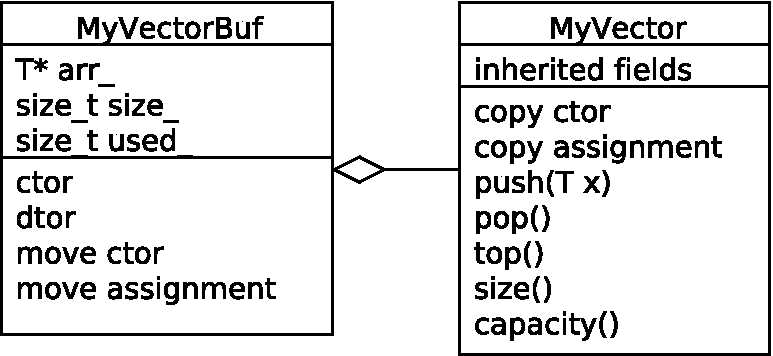
\includegraphics[width=0.6\textwidth]{illustrations/myvector-crop.pdf}
\caption{Диаграмма классов двухуровневого буфера}
\label{fig:my_vector}
\end{figure}

Основная идея показана на (рис. \ref{fig:my_vector}). Все поля хранятся в \lstinline!MyVectorBuf!.

\begin{lstlisting}
template <typename T>
struct MyVectorBuf 
{
  MyVectorBuf(const MyVectorBuf&) = delete;
  MyVectorBuf& operator= (const MyVectorBuf&) = delete;
protected:
  T *arr_;
  size_t size_, used_;
// .... etc ....
\end{lstlisting}

Очень важно, что базовый класс не является копируемым. Это позволяет избежать всех проблем, связанных с копированием по умолчанию.

Конструктор и деструктор просто выделяют и освобождают сырую память.

\begin{lstlisting}
MyVectorBuf(size_t sz = 0) : 
  arr_((sz == 0) ? nullptr : 
    static_cast<T*>(::operator new(sizeof(T) * sz))), 
  size_(sz), used_(0) {}

~MyVectorBuf() noexcept {
  destroy(arr_, arr_ + used_);
  ::operator delete(arr_);
}
\end{lstlisting}

На самом деле специально помечать деструктор как \lstinline!noexcept! не нужно, начиная с C++11 все деструкторы помечены так автоматически.

Функция \lstinline!destroy!, использованная здесь была описана чуть выше. Перемещение и перемещающимй конструктор тривиальны.

Базовый класс \lstinline!MyVectorBuf! связан с наследником \lstinline!MyVector! закрытым наследованием как показано ниже.

\begin{lstlisting}
template <typename T> struct MyVector : 
                       private MyVectorBuf<T> 
{
  using MyVectorBuf<T>::used_;
  using MyVectorBuf<T>::size_;
  using MyVectorBuf<T>::arr_;
// .... etc ....
\end{lstlisting}

Разумеется, закрытое наследование это и есть композиция. Собственно можно обойтись без него и сделать композицию явной, но ценой некоторого неудобства дальнейших записей (\lstinline!buf.used_! вместо \lstinline!used_! и т.п.).

Теперь копирующий конструктор выглядит изящно и не требует catch-all

\begin{lstlisting}
MyVector (const MyVector &rhs) : MyVectorBuf<T>(rhs.used_)  {
  while (used_ < rhs.used_) {
    construct (arr_ + used_, rhs.arr_[used_]);
    used_ += 1;
  }
}
\end{lstlisting}

Функция \lstinline!construct! это просто обёртка над размещающим \lstinline!new! и была показана ранее. Здесь следует остановиться подробней, потому что именно в этот момент становится ясна красота замысла.

Что будет, если внутри \lstinline!construct! возникнет исключение? Ничего страшного, поскольку теперь память будет корректно освобождена деструктором базового подобъекта.

Очень красиво также выглядит метод \lstinline!MyVector::push! в такой архитектуре

\begin{lstlisting}
void push(T t) {
  if (used_ == size_) {
    MyVector tmp (size_*2 + 1);
    while (tmp.size() < used_)
      tmp.push(arr_[tmp.size()]);
    tmp.push(t);
// -------------- Kalb line -----
    swap(*this, tmp);
    return;
  }
  construct(arr_ + used_, t);
  used_ += 1;
}
\end{lstlisting}

Комментарием в коде помечена линия, которая называется ``линией Калба'' (Kalb line). Это полезная идиома при проектировании безопасного кода. Считается, что выше линии Калба код может генерировать исключения, но не влияет на состояние класса, а ниже неё -- влияет на состояние, но не генерирует исключений.

Итак, хорошее проектирование кода позволяет сделать его безопасным относительно исключений. Примерно таким образом будет устроена большая часть контейнеров стандартной библиотеки.

Конечно реализовать всё это можно только если есть хотя бы некоторые функции, такие как \lstinline!swap!, которые отвечают гарантии бессбойности и не кидают исключений никогда.

Что если пойти дальше и распространить бессбойность на прочие части кода?

\subsection{Жизнь без исключений}\label{subsub:noexcept}

Кое что о спецификаторе \lstinline!noexcept! уже было рассказано (см. \ref{subsub:basic_noexcept}) но уже в расках этого раздела мы несколько раз были вынуждены обратиться к гарантии бессбойности, в основном в коде деструкторов или коде, который используется деструкторами (таком как функция \lstinline!destroy!).

На самом деле, многие интересные возможности использовать \lstinline!noexcept! были пропущены (по определённым причинам).

Можно ещё разок посмотреть на метод \lstinline!push! и на то как он копирует объекты в новую память:

\begin{lstlisting}
MyVector tmp (size_*2 + 1);
while (tmp.size() < used_)
  tmp.push(arr_[tmp.size()]);
tmp.push(t);
// -------------- Kalb line -----
swap(*this, tmp);
return;
\end{lstlisting}

Это подозрительный код, потому что непонятно зачем \textbf{копировать} нечто, что потом сразу же будет уничтожено? Почему не \textbf{перемещать} это? С перемещением всё выглядит чуть лучше

\begin{lstlisting}
MyVector tmp (size_*2 + 1);
while (tmp.size() < used_)
  tmp.emplace(move(arr_[tmp.size()]));
tmp.emplace(move(t));
// -------------- Kalb line -----
swap(*this, tmp);
return;
\end{lstlisting}

Но некоторым оверхедом выглядит тот факт, что перемещение делается дважды. Первый раз при заполнении \lstinline!tmp!, а второй раз в перемещающем присваивании, когда будет отрабатывать \lstinline!swap!.

Можно улучшить время ещё вдвое если просто выделить на \lstinline!arr_! больше памяти и заполнить сразу её. В этом случае, конечно, непонятно, что делать с исключениями, если они вылетят при перемещающем присваивании.

Но что если они не вылетят?

Кажется здесь есть возможность действовать двумя способами: более консервативным, если перемещающее присваивание порождает исключения и менее консервативным, если оно их не порождает. Для того, чтобы отличать такие случаи, в язык был введен оператор \lstinline!noexcept(X)! который возвращает \lstinline!true! или \lstinline!false! в зависимости от того, может выражение \lstinline!X! бросить исключение или не может. А сама аннотация \lstinline!noexcept! для метода сделана условной.

В итоге если есть странная функция, которую непонятно помечать \lstinline!noexcept! или нет, например такая:

\begin{lstlisting}
template <class T>
T copy(T const& original) // noexcept?
{
  return original;
}
\end{lstlisting}

То, во-первых можно использовать условный \lstinline!noexcept! обратив внимание, что для фундаментальных типов тут явно не будет сбоев

\begin{lstlisting}
template <class T>
T copy(T const& original) noexcept(is_fundamental<T>::value)
{
  return original;
}
\end{lstlisting}

А во-вторых (и это лучший вариант), можно просто использовать оператор внутри условной директивы и сказать, что какой бы ни был тип, если его копирование не порождает исключений, то и эта функция тоже не должна.

\begin{lstlisting}
template <class T>
T copy(T const& original) noexcept(noexcept(T(original)))
{
  return original;
}
\end{lstlisting}

Оператор \lstinline!noexcept! оценивает каждую функцию, задействованную в выражении, но не вычисляет выражение

\begin{lstlisting}
struct ThrowingCtor { ThrowingCtor(){} };
void foo (ThrowingCtor) noexcept;
void foo (int) noexcept;
assert (noexcept (foo(1)) == true);
assert (noexcept (foo(ThrowingCtor{})) == false);
\end{lstlisting}

Разумеется он также возвращает false для constant expressions

\textbf{Домашняя наработка:} переписать метод \lstinline!push! в двух SFINAE перегрузках, используя условный \lstinline!noexcept!.

Жизнь без исключений не означает полного отказа от обработки ошибок. Для ошибок, которые могут быть обработаны на том же уровне прекрасно работают старые добрые коды возврата, которые в C++11 были даже улучшены с помощью нового заголовочного файла \lstinline!<system_error>!.

Новые стандартные типы \lstinline!error_code! и \lstinline!error_category! и список стандартных категорий в пространстве имён \lstinline!std::errc! дают возможность унифицировать семантические группы кодов ошибок (как это делается например при ловле исключений по базовому классу).

\begin{lstlisting}
error_code ec { MY_OUTOF_MEM, errc::not_enough_memory };
\end{lstlisting}

Здесь errc это категория ошибки, а \lstinline!error_code! может быть платформенно зависимым. Теперь сравнение на равенство сравнит код со своей группой

\begin{lstlisting}
if (ec == errc::not_enough_memory) {
  // process not enough memory
}
\end{lstlisting}

Использование перегрузки по кодам ошибки позволяет иметь две функции, одна из которых бросает исключения а вторая сообщает код ошибки в одном классе.

\begin{lstlisting}
void push (T new_elem);
void push (T new_elem, error_code &ec) noexcept;
\end{lstlisting}

На самом деле заголовочный файл \lstinline!<system_error>! гораздо больше и интересней. Интересующиеся студенты могут изучить его на досуге и доложить результаты, например на семинаре.

%TODO: есть некие дополнительные главы по исключениям: заворачивание в \lstinline!exception_ptr!, вкладывание через \lstinline!throw_with_nested! и выяснение того идёт или вопрямща размотка стека через \lstinline!uncaught_exception!. Непонятно надо ли делать отдельный подраздел  по этим возможностям, поскольку реально ими никто не пользуется же особо. Подумать.

\pagebreak
\section{Умные и слишком умные указатели}\label{SmartPointers}

\hfill\textit{Manual lifetime management really can seem akin}

\hfill\textit{to constructing a mnemonic memory circuit}

\hfill\textit{using stone knives and bear skins}{\vspace{0.5em}}

\hfill\textit{-- Scott Meyers}

Идиома RAII уже рассматривалась в (\ref{RAII}), и там же была сделана наивная попытка завернуть в класс для управления ресурсами такой классический разделяемый ресурс как дисковый файл. Конечно, идея обобщить RAII для любого \lstinline!T!, используя шаблоны -- приходит на ум почти сразу после знакомства с шаблонами.

\begin{lstlisting}
template <typename U>
int foo (int x) {
  U *ptr = new U(x);
  // .... some code ....
  if (some condition) {
    delete ptr; 
    return -1;
  }
  // .....
  delete ptr;
  return 0;
}
\end{lstlisting}

Этот мотивирующий пример плох, кажется, вообще всем: здесь ручное управление ресурсами с дублированием кода, здесь небезопасность относительно исключений и всё такое.

Хотелось бы завернуть это в некую симпатичную RAII обёртку

\begin{lstlisting}
template <typename U>
int foo (int x) {
  RAIIPtr<U> ptr(new U(x));
  // .... some code ....
  if (some condition) {
    return -1;
  }
  // .....
  return 0;
}
\end{lstlisting}

Паттерн обертки, осуществляющей управление временем жизни объекта умнее, чем это делается через обычный указатель, называется ``smart pointer'' или умный указатель. Таким образом это не какой-то класс, это общая концепция для целого семейства от крайне простых до крайне сложных и интересных классов.

\subsection{Первая попытка -- не слишком умный указатель}

Первая попытка написать не слишком сложную обертку для управления ресурсами, может выглядеть как-то так:

\begin{lstlisting}
template <typename T> class RAIIPtr {
  T *ptr_;
public:
  RAIIPtr(T *ptr = nullptr) : ptr_(ptr) {}
  ~RAIIPtr() { delete ptr_; }
  T operator*() const { return *ptr_; }
  T* operator->() const { return ptr_; }
};
\end{lstlisting}

Перегрузка двух интересных операторов -- \lstinline!operator*! (dereferencing, разыменование) и \lstinline!operator->! (indirection, косвенный доступ) уже обсуждалась ранее (см. \ref{OperatorOverloading}).

Тем не менее, в коде выше есть проблема и она становится очевидной, если посмотреть на него через ``волшебные очки'' (про этот удивительно полезный девайс, см. \ref{subsub:magicglasses}).

\begin{lstlisting}
template <typename T> class RAIIPtr {
  T *ptr_;
public:
  RAIIPtr(T *ptr = nullptr) : ptr_(ptr) {}
  ~RAIIPtr() { delete ptr_; }
  RAIIPtr(const RAIIPtr&) = default;
  RAIIPtr& operator= (const RAIIPtr&) = default;
  T operator*() const { return *ptr_; }
  T* operator->() const { return ptr_; }
};
\end{lstlisting}

Теперь должно быть очевидно, что обычное копирование или создание по образцу такого указателя приведет к ошибке двойного удаления (см. \ref{RAII}, где эта проблема изложена подробно). 

Конечно, если содержимое может быть скопировано, его можно скопировать. Это подход неинтрузивных контейнеров, таких как vector или string. Но в общем случае содержимое не может быть так просто скопировано. Что тут можно сделать? 

Самый простой способ -- запретить копирование и присваивание. 

\begin{lstlisting}
template <typename T> class SRAIIPtr {
  T *ptr_;
public:
  SRAIIPtr(T *ptr = nullptr) : ptr_(ptr) {}
  ~SRAIIPtr() { delete ptr_; }
  SRAIIPtr(const SRAIIPtr&) = delete;
  SRAIIPtr& operator= (const SRAIIPtr&) = delete;
  T operator*() const { return *ptr_; }
  T* operator->() const { return ptr_; }
};
\end{lstlisting}

Эта стратегия называется ``scoped pointer'' и именно так устроен и работает класс \lstinline!boost::scoped_ptr!. Таким образом, можно даже не писать велосипед

\begin{lstlisting}
template <typename U>
int foo (int x) {
  boost::scoped_ptr<U> ptr(new U(x));
  // .... some code ....
  if (some condition) {
    return -1;
  }
  // .....
  return 0;
}
\end{lstlisting}

Отдельный вопрос: почему ничего такого не было включено в стандарт, но он получит своё ответ далее. Итак, простейшая проблема, таким образом решена. Пора перейти к более сложным случаям. А конкретно: к случаям, когда указатель вынужден утекать из области видимости.

\subsection{Автоматические указатели и их проблемы}\label{COAP}

Иногда указатели могут ``утекать'' за scope. Это вполне естественно и нормально и логично иметь нормальные способы это обработать. Пример, приведённый ранее может быть расширен следующим образом:

\begin{lstlisting}
template <typename T> bar(T*);

template <typename U>
int foo (int x) {
  boost::scoped_ptr<U> ptr(new U(x));
  // .... some code ....
  if (some condition) {
    bar<U>(ptr.get());
  }
  // .....
  return 0;
}
\end{lstlisting}

Увы, это очень плохая идея. В строчке вызова функции bar утекает сырой указатель. Теперь мы совсем не можем быть уверены, что его никто не освободит там, куда он утёк, и уж точно никак не можем это проконтролировать.

Древним выходом из этой ситуации является \lstinline!auto_ptr!. Введённый в 98 стандарте, этот указатель определял конструктор копирования через передачу владения ресурсом

\begin{lstlisting}
ARAIIPtr(ARAIIPtr& rhs) : ptr_(rhs.ptr_) { 
  rhs.ptr_ = nullptr; 
}
ARAIIPtr& operator= (ARAIIPtr rhs) { 
  swap(*this, rhs); return *this; 
}
\end{lstlisting}

Такой подход позволяет эффективно решить проблему: теперь нет нужды позволять утекать голому указателю, он передаётся вместе с владением

\begin{lstlisting}
template <typename T> bar(auto_ptr<T>);

template <typename U>
int foo (int x) {
  auto_ptr<U> ptr(new U(x));
  // .... some code ....
  if (some condition) {
    bar<U>(ptr);
  }
  // .....
  return 0;
}
\end{lstlisting}

Увы, передача владения таким образом подразумевает, в некотором смысле \textbf{слишком} тихое копирование. Типичный случай: пусть есть класс, который делает внутри себя резервную копию своего аргумента.

\begin{lstlisting}
template <typename T>  struct Brittle {
  T working_, reserve_;
  Brittle (T val) : working_(val), reserve_(working_) {}
};
\end{lstlisting}

Попытка использовать этот класс, параметризованный \lstinline!auto_ptr! приведёт к удивительным и разрушительным последствиям.

\begin{lstlisting}
Brittle<auto_ptr<int>> b (auto_ptr<int>(new int(42)));
\end{lstlisting}

Очень плохо то, что это скомпилируется без каких-нибудь ошибок, управление логично и закономерно утечёт в резервную копию, рабочая копия останется пустой и потом, где-нибудь это выстрелит.

Но самым-самым плохим является то, что приведённый выше класс \lstinline!Brittle! очень напоминает неинтрузивные контейнеры стандартной библиотеки, которые по сути делают всё то же самое, только ещё сложнее.

Любые попытки использовать \lstinline!auto_ptr! со стандартными контейнерами опасны и порочны. Специальное сокращение COAP\index{COAP} расшифровывающееся как ``container of auto ptrs'' долгое время было синонимом таящегося и абсолютного зла.

При очевидной полезности \lstinline!auto_ptr!, поражает воображение его способность разрушать и приводить в негодность самые невинно выглядящие контексты. Никто не заподозрил бы экземпляр COAP в приведённом выше классе Brittle, он же совсем не похож на классические контейнеры.

Отчаяние и безысходность продолжались до 2011 года, когда стандарт был наконец пересмотрен в сторону введения так называемой семантики перемещения (см. \ref{subsub:movesemantics}), которая, в свою очередь, позволила ввести настоящую абстракцию я уникального владения ресурсом -- unique pointers.

\subsection{Уникальное владение}\label{subsub:uniqueptrs}

\hfill\textit{I'm the one that has to die}

\hfill\textit{when it's time for me to die}{\vspace{0.5em}}

\hfill\textit{-- Jimi Hendrix}

Если вдуматься, основная проблема использования копирования для передачи владения ресурсом -- не в самой передаче владения, а именно в том, что для этого используется копирование, которое просто семантически для этого не предназначено.

Соответственно с появлением перемещающего присваивания, естественный выход из ситуации это запретить копирование, но открыть перемещение.

\begin{lstlisting}
URAIIPtr(const URAIIPtr&) = delete;
URAIIPtr& operator= (const URAIIPtr&) = delete;
URAIIPtr(URAIIPtr&& rhs) : ptr_(rhs.ptr_) { 
  rhs.ptr_ = nullptr; 
} 
URAIIPtr& operator= (URAIIPtr&& rhs) { 
  swap(*this, rhs); return *this; 
}
\end{lstlisting}

Эта идея позволяет решить проблему передачи ресурса за пределы области видимости.

\begin{lstlisting}
template <typename T> bar(unique_ptr<T>);

template <typename U>
int foo (int x) {
  auto ptr = make_unique<U>(x);
  // .... some code ....
  if (some condition) {
    bar<U>(move(ptr));
  }
  // .....
  return 0;
}
\end{lstlisting}

Здесь следует в первую очередь обратить внимание на использование \lstinline!std::move!. Теперь передача ресурса это действительно и явно перемещающая передача.

А что насчёт \lstinline!Brittle! -- может тут спросить внимательный читатель.

\begin{lstlisting}
Brittle<unique_ptr<int>> b (unique_ptr<int>(new int(42)));
\end{lstlisting}

Разумеется коварная строчка из предыдущего раздела даже не скомпилируется.

Также стоит обратить внимание на метод создания указателя. Тут есть два варианта: классический через конструктор и использованный выше.

\begin{lstlisting}
auto ptr = make_unique<U>(x);
unique_ptr<U> ptr (new U(x));
\end{lstlisting}

В данном случае они посимвольно равны в записи. Тем не менее, разница есть и кроется в основном в вопросах безопасности исключений. Если new отработало, а потом конструктор \lstinline!unique_ptr! бросил исключение, то выделенная память утечёт.

Единственное, что сначала кажется неудобным это аллокация массива. Кажется, что в конструкторе можно написать

\begin{lstlisting}
unique_ptr<int> ptr (new int[1000]()); // ERROR
\end{lstlisting}

Тогда как \lstinline!make_unique! этого не позволяет. Но это, пожалуй, аргумент за \lstinline!make_unique!. Потому что такая запись является грубой ошибкой. И действительно: тут смешаны формы \lstinline!new[]! и \lstinline!delete!.

Есть два варианта корректно аллоцировать массив и оба используют специализацию шаблона для массивов.

\begin{lstlisting}
auto ui = make_unique<int[]>(1000);
unique_ptr<int[]> ui (new int[1000]());
\end{lstlisting}

Теперь правильно спарены \lstinline!new[]! и \lstinline!delete[]!. Если записать такую схему в велосипеде \lstinline!URAIIPtr!, она будет выглядеть следующим образом.

Во-первых удалитель теперь будет параметром шаблона

\begin{lstlisting}
template <typename T, typename Deleter = default_delete<T>> 
class URAIIPtr {
  T *ptr_;
  Deleter del_;
public:
  URAIIPtr(T *ptr = nullptr, Deleter del = Deleter()) :
    ptr_(ptr), del_(del) {}
  ~URAIIPtr() { del_(ptr_); }
\end{lstlisting}

Во-вторых он будет частично специализирован

\begin{lstlisting}
template <typename T> struct default_delete {
  void operator() (T *ptr) { delete ptr; }
};

template <typename T> struct default_delete<T[]> {
  void operator() (T *ptr) { delete [] ptr; }
};
\end{lstlisting}

Разумеется, в такой системе кажется, что есть третий выход: воспользоваться своим удалителем.

\textbf{Вопрос к студентам:} напишите свой удалитель к некорректному варианту, использующему \lstinline!unique_ptr<int>! и при этом \lstinline!new int[1000]()! в конструкторе так, чтобы этот вариант заработал.

\ifanswers
Правильный ответ: например так

\begin{lstlisting}
template <typename T> struct MyArrDeleter {
  void operator()(T *t) { delete [] t; }
};

unique_ptr<int, MyArrDeleter<int>> ui3 (new int[1000]());
\end{lstlisting}

Но хороший студент напишет через лямбду
\fi

Пользовательский удалитель может быть сколь угодно сложным: класс с нетривиальным конструктором, лямбда с захватом контекста. Но чаще всего нужны старые добрые сишные функции.

\begin{lstlisting}
Resource *create();
void destroy(Resource *);
unique_ptr<Resource, decltype(&destroy)> ures (create(), destroy);
\end{lstlisting}

Увы, в этом случае пользователь платит штраф на размер указателя, который теперь вынужденно включает указатель на функцию.

\textbf{Вопрос к студентам:} что вы думаете про \lstinline!unique_ptr<void>!, можно ли его использовать как уникальный обобщённый указатель?

\ifanswers
Проблемы, как водится, будут с удалением. Работать может примерно такая городушка:

\begin{lstlisting}
template <typename T>
struct VDel {
  void operator()(void *s) { delete static_cast<T*>(s); }
};
unique_ptr<void, VDel<int>> u(new int(42));
\end{lstlisting}
\fi

Очень часто люди, узнав про \lstinline!unique_ptr! радуются (правильно радуются) и заменяют им голые указатели члены в своих классах (правильно заменяют). Но при этом часто возникает проблема с предварительными объявлениями.

\begin{lstlisting}
class MyClass; // forward declared
\end{lstlisting}

В этом случае старый вариант не составляет проблем.

\begin{lstlisting}
struct MyWrapper {
  MyClass *c;
  MyWrapper() : c(nullptr) {};
};
\end{lstlisting}

В то же время новый вариант не компилируется.

\begin{lstlisting}
// FAIL!
struct MySafeWrapper {
  unique_ptr<MyClass> c; 
  MySafeWrapper() : c(nullptr) {};
};
\end{lstlisting}

Проблема состоит в том, что дефолтный удалитель просачивается в хедер и приносит туда вызов \lstinline!delete!, а этот вызов для неполных типов не работает.

Разумеется проблема может быть решена кастомным удалителем

\begin{lstlisting}
struct MyClassDeleter {
  void operator()(MyClass *p);
};

struct MySafeWrapper { 
  unique_ptr<MyClass, MyClassDeleter> c; 
  MySafeWrapper() : c(nullptr) {}
};
\end{lstlisting}

\textbf{Вопрос к студентам:} видите ли вы иные способы решить проблему?
\ifanswers
Правильный ответ: да, например не определять конструктор в хедере.
\fi

\subsection{Проектирование с уникальными указателями}\label{subsub:uniquetrees}

Идиома PImpl уже рассматривалась в связи с исключениями и является хорошим и заслуженным инструментом программиста, средством своего рода ``гальванической развязки'' интерфейса с реализацией, за которую мы иногда согласны пожертвовать один уровень косвенности при обращениях.

Не может ли эта идиома быть существенно улучшена с использованием умных указателей? Конечно может. Итак, допустим исходный код представляет классический PImpl.

\begin{lstlisting}
class Ifacade {
  CImpl *const impl_;
public:
  Ifacade() : impl_(new CImpl) {}  
  // ..... other methods
};
\end{lstlisting}

\textbf{Вопрос к студентам:} понимаете ли вы почему указатель лучше держать константным?

\ifanswers
Правильный ответ: например чтобы не забыть его инициализировать и чтобы заблокировать всякие копирующие и прочие конструкторы по умолчанию
\fi

Переход от неё к уникальному владению довольно прост.

\begin{lstlisting}
class Ifacade {
  const unique_ptr<CImpl> impl_;
public:
  Ifacade() : impl_(new CImpl) {}
  // ..... other methods
};
\end{lstlisting}

К слову можно упомянуть тот факт, что \lstinline!const unique_ptr! это идеальный \lstinline!scoped_ptr!. И действительно: он никак даже случайно не может быть ни скопирован ни (он же const) перемещён.

Что если класс управляет не одним, а более указателями. Например если это дерево? Дерево уникальных указателей выглядит крайне просто и естественно.

\begin{lstlisting}
template <typename Data> class Tree {
  struct Node {
    unique_ptr<Node> left, right;
    Data d;
  };
  unique_ptr<Node> top_;
  void release_subtree(unique_ptr<Node> u) {}
  // ..... other 42 methods ......
};
\end{lstlisting}

Обратите внимание на реализацию метода \lstinline!release_subtree!, она довольно симпатична. Почему это работает? Потому что сдвинутый туда уникальный указатель оказывается в этой области видимости и по выходе из неё уничтожается.

TODO: Про возможное переполнение стека при удалении и про решение

\begin{lstlisting}
void release_subtree(unique_ptr<Node> u) {
  // TODO: нетривиальное решение тут
}  
\end{lstlisting}

\textbf{Вопрос к студентам:} Можно ли (если да то как и если нет, то почему) сделать на \lstinline!unique_ptr! направленный ациклический граф?

\subsection{Совместное владение}\label{subsub:sharedptrs}

\hfill\textit{A shared pointer is as good as a global variable} {\vspace{0.5em}}

\hfill\textit{-- Sean Parent}

К сожалению, с деревом всё гладко лишь до тех пор, пока оно инкапсулировано. Но что если нужен метод, который ищет узел в дереве и отдаёт указатель на него внешнему владельцу? Не хотелось бы вместе с узлом передавать всё поддерево, исключая его из дерева. Также позволять утекать сырому указателю совсем не хочется.

Решением может быть: вернуть указатель с совместным владением.

\begin{lstlisting}
template <typename Data> class Tree {
  struct Node {
    shared_ptr<Node> left, right;
    Data d;
  };
  shared_ptr<Node> top_;
public: 
  shared_ptr<Node> find (int inorder_pos) {
    shared_ptr<Node> spn;
    // searching
    return spn;
  }
\end{lstlisting}

Что это за указатель с разделяемым владением?

Можно вспомнить основную проблему RAII: копирование. Пока что были рассмотрены первые три выхода, указатели с разделяемым использованием открывают четвёртый вариант.

\begin{enumerate}
\item Отказ от копирования: \lstinline!scoped_ptr!, \lstinline!const unique_ptr!
\item Копирование с передачей владения \lstinline!auto_ptr!
\item Перемещение с передачей владения \lstinline!unique_ptr!
\item Копирование с подсчётом ссылок и удалением при обнулении счётчика \lstinline!shared_ptr! 
\end{enumerate}

Принципиальная схема разделяемого указателя приведена на (рис. \ref{fig:smartptrs-outer}).

\begin{figure}[ht]
\centering
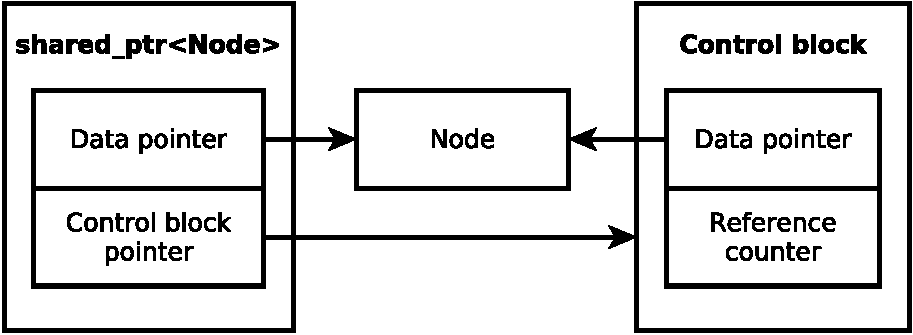
\includegraphics[width=1.0\textwidth]{illustrations/smartptrs-outer-crop.pdf}
\caption{Разделяемые указатели: контрольный блок}
\label{fig:smartptrs-outer}
\end{figure}

Этой картинке не стоит чрезмерно верить, её уточнение -- дело ближайшего времени. Основные элементы картинки это данные, которые сохраняются в куче пока счётчик ненулевой, контрольный блок, который выделен отдельно и содержит счётчик и указатель на данные и конкретные разделяемые указатели, которые ссылаются на контрольный блок.

Существует (начиная с C++14) два способа создать разделяемый указатель.

\begin{enumerate}
\item С помощью конструктора 
\begin{lstlisting}
shared_ptr<Node> p2(new Node());
\end{lstlisting}
\item С помощью специальной функции \lstinline!make_shared!
\begin{lstlisting}
shared_ptr<Node> p1 = make_shared<Node>();
\end{lstlisting}
\end{enumerate}

В первом случае данные и контрольный блок создаются двумя разными выделениями и существуют отдельно, как это и показано на (рис. \ref{fig:smartptrs-outer}). Этот вариант менее эффективен и менее безопасен относительно исключений, чем второй вариант, когда данные и контрольный блок создаются одним выделением динамической памяти (см. рис. \ref{fig:smartptrs-inner}).

\begin{figure}[ht]
\centering
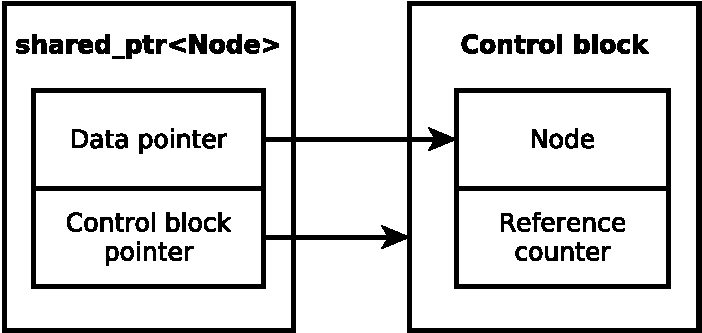
\includegraphics[width=1.0\textwidth]{illustrations/smartptrs-inner-crop.pdf}
\caption{Устройство разделяемого указателя после make\_shared}
\label{fig:smartptrs-inner}
\end{figure}

Метод через \lstinline!make_shared! не сработает если в классе есть закрытые или защищённые конструкторы.

\begin{lstlisting}
class A {
  int val;
  A(int v): val(v){}
public:
  shared_ptr<A> createNext(){ 
    return make_shared<A>(val); // FAIL 
  }
  shared_ptr<A> createNext(){ 
    return shared_ptr<A>(new A(val)); } // OK
  };
// ......
\end{lstlisting}

Проблема очевидна: \lstinline!make_shared! не друг класса и не имеет доступа к его непубличной части.

Возвращаясь к проблеме метода find, можно заметить, что он возвращает слишком много. Что если нужна не вся нода, а только указатель на данные из неё и всё-таки не хочется делать его сырым указателем?

\begin{lstlisting}
template <typename Data> class Tree {
  struct Node {
    shared_ptr<Node> left, right;
    Data d;
  };
  shared_ptr<Node> top_;
public: 
  shared_ptr<Data> find (int inorder_pos) {
    shared_ptr<Node> spn;
    // ..... searching ....
    return {spn, &(spn->d)};
  }
\end{lstlisting}

Этот способ создания называется созданием с алиасингом (aliasing constructor) и проиллюстрирован на (рис. \ref{fig:smartptrs-aliased})

\begin{figure}[ht]
\centering
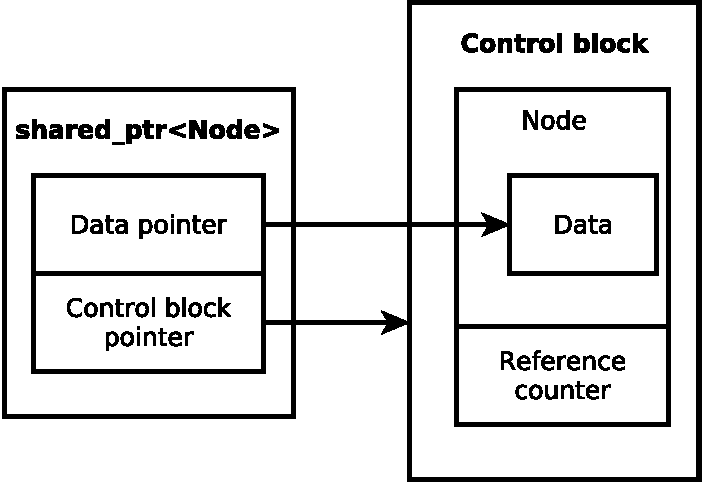
\includegraphics[width=1.0\textwidth]{illustrations/smartptrs-aliased-crop.pdf}
\caption{Алиасинг в разделяемых указателях}
\label{fig:smartptrs-aliased}
\end{figure}

Благодаря созданию с алиасингом, указатель может ссылаться на часть данных, управляемых его контрольным блоком, а не на все данные.

Разумеется, само наличие контрольного блока (подозрительно напоминающего похороненную было корову, см. \ref{subsub:cow}) может стать проблемой per se. Например может быть такое, что два разных разделяемых указателя были сделаны из одного.

\begin{lstlisting}
Node *n = new Node();
shared_ptr<Node> spn1(n);
shared_ptr<Node> spn2(n);
\end{lstlisting}

Это приводит к созданию двух контрольных блоков и той же проблеме двойного удаления, от которой исходно пытались уйти с помощью подсчёта ссылок

И в общем такие ситуации это ещё один аргумент за \lstinline!make_shared!, который исключает эти проблемы.

Тем не менее, редко попадаясь на приведённый выше абсурдный сценарий, люди часто попадаются на него же, но когда указателем является this. Следующий фрагмент кода куда сложнее выкупить.

\begin{lstlisting}
struct Node {
  shared_ptr<Node> getspn() {
    return shared_ptr<Node>(this); // ouch
  }
};

shared_ptr<Node> bp1 = make_shared<Node>();
shared_ptr<Node> bp2 = bp1->getspn();
\end{lstlisting}

Правильная стратегия действий использует CRTP (см. \ref{CRTP}). В класс, который хочет экспортировать указатель на самого себя подмешивается шаблонная добавка \lstinline!enable_shared_from_this!, добавляющая в класс специальный метод \lstinline!shared_from_this()!

\begin{lstlisting}
struct Node: enable_shared_from_this<Node> {
  shared_ptr<Node> getspn() {
    return shared_from_this();
  }
};
\end{lstlisting}

О том как это работает говорить пока рано, так как используется механизм слабых указателей, (см. \ref{subsub:weakptrs})

\begin{lstlisting}
Node n; // shall be owned
shared_ptr<Node> gp1 = n.getptr(); // UB
\end{lstlisting}

Впрочем это UB остаётся UB только до C++17. Начиная с 2017 года это выбрасывает исключение \lstinline!std::bad_weak_ptr!.

Обычные указатели ковариантны и это довольно удобно, так как между ними можно статически переходить.

\begin{lstlisting}
class A {};
class B : public A {};
B *b = new B();
A *a = static_cast<A*>(b);
\end{lstlisting}

Чтобы сохранить это свойство, статическое преобразование было сделано специально для разделяемых указателей (название \lstinline!static_pointer_cast! не слишком удачное, так как он не действует для \lstinline!unique_ptr! и прочих).

\begin{lstlisting}
shared_ptr<B> b = make_shared<B>();
shared_ptr<A> a = static_pointer_cast<A>(b);
\end{lstlisting}

Аналогично работают \lstinline!dynamic_pointer_cast! и \lstinline!const_pointer_cast!, имитируя известные приведения.

TODO: пользовательские удалители

\subsection{Слабые указатели}\label{subsub:weakptrs}

Главная проблема указателей с совместным владением это возможность циркулярных ссылок. Следующий код выглядит безобидно, но создаёт утечку памяти.

\begin{lstlisting}
struct Node {
  shared_ptr<Node> parent, left, right;
};

{
  shared_ptr<Node> master = make_shared<Node>();
  shared_ptr<Node> slave = make_shared<Node>();
  slave.parent = master;
  master.left = slave;
} // LEAK
\end{lstlisting}

Давайте разберём в деталях что тут происходит. Сначала создаётся указатель на master и его счётчик ссылок равен единице. Далее то же самое происходит для slave. Далее slave устанавливает совместный указатель на родителя, используя для этого существующий master. Количество ссылок в контрольном блоке master становится равно двум. Далее master ставит slave своим левым потомком, увеличивая счётчик ссылок в его контрольном блоке до двух.

Далее самое интересное. Завершается область видимости. Что происходит? Объекты master и slave выходят из зоны видимости, их счётчики уменьшаются на единицу. Но сами они от этого не умирают, так как кросс-ссылки на контрольные блоки продолжают держать их живыми.

И это не какие-то баги в реализации. Всё дело в отношении владения. Когда оно взаимное, оно создаёт крайне живучую конструкцию.

Выход из ситуации: заменить указатель наверх на невладеющий указатель.

\begin{lstlisting}
struct Node {
  weak_ptr<Node> parent
  shared_ptr<Node> left, right;
};
\end{lstlisting}

Идея слабого указателя и получающийся при этом вид контрольного блока показаны на (рис. \ref{fig:smartptrs-weak-outer}). Здесь в контрольном блоке пропущены пользовательские удалители (которых в данном случае в общем и нет), зато показан так называемый счётчик слабых ссылок.

\begin{figure}[ht]
\centering
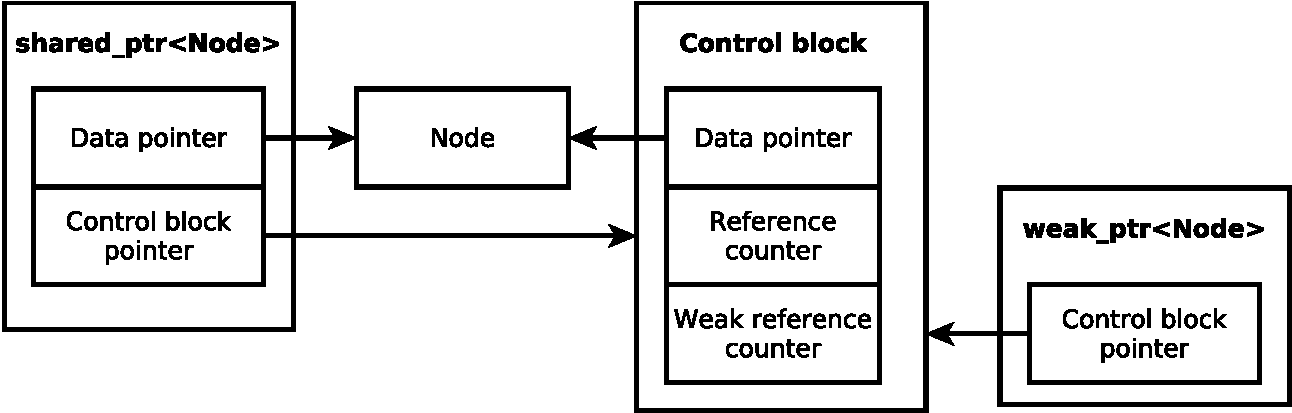
\includegraphics[width=1.0\textwidth]{illustrations/smartptrs-weak-outer-crop.pdf}
\caption{Слабые указатели и устройство контрольного блока}
\label{fig:smartptrs-weak-outer}
\end{figure}

При рассматривании рисунка возникает закономерная мысль: почему слабый указатель хранит только указатель на контрольный блок? Правильный ответ: потому что его \textbf{нельзя разыменовать}.

\begin{lstlisting}
auto t = make_shared<int>(42);
weak_ptr<int> w = t;
int xt = *t; // OK
int xw = *w; // CE
\end{lstlisting}

Всё, что можно сделать со слабым указателем это атомарно ``защёлкнуть'' его, превратив в сильный и только потом разыменовать.

\begin{lstlisting}
auto tprime = w.lock();
int xtp = *tprime;
\end{lstlisting}

Защёлкивание не вовремя может создать те же проблемы циклической ссылки, но они более контролируемы. Например временно защёлкнуть указатель parent у структуры Node приведённой выше -- практически безопасно.

Тем не менее, наличие слабых ссылок выявляет неожиданный аргумент против \lstinline!make_shared!. Идея показана на (рис. \ref{fig:smartptrs-weak-inner}).

\begin{figure}[ht]
\centering
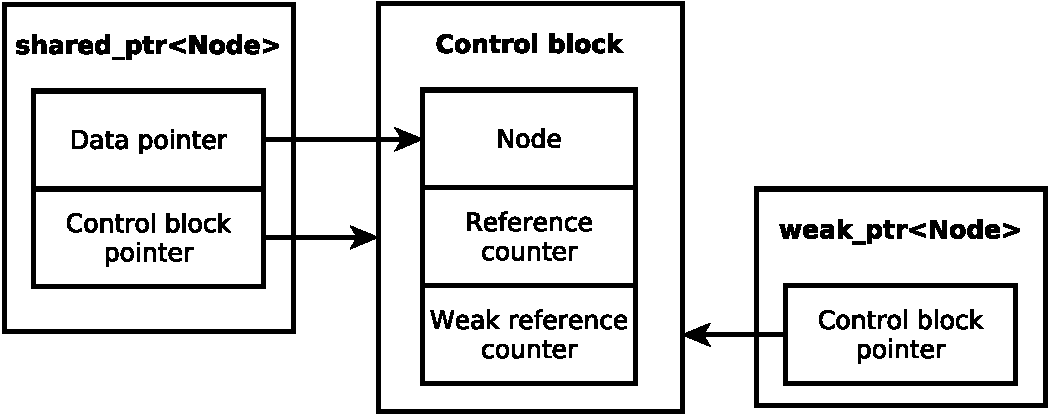
\includegraphics[width=1.0\textwidth]{illustrations/smartptrs-weak-inner-crop.pdf}
\caption{Проблема make\_shared и слабых ссылок}
\label{fig:smartptrs-weak-inner}
\end{figure}

Здесь блок был выделен с помощью одного выделения вместе с данными и на него есть и сильные и слабые ссылки. Если на блок не останется ни одной сильной ссылки, то что произойдёт?

\begin{itemize} 
\item Control block живёт пока есть слабые ссылки
\item Data освобождается
\item Data pointer становится nullptr
\item Если weak pointer указывает на control block без сильных ссылок, то он expired
\end{itemize} 

Интересный термин expired (истёк) требует разбора. Обычный указатель может повиснуть если то, на что он указывал было удалено. Но слабый указатель не провисает. Он истекает и это можно детерминированно проверить.

\begin{lstlisting}
weak_ptr<int> 
foo () 
{
  auto res = make_shared<int>(42);
  return res;
} // expiration

weak_ptr<int> result = foo();
assert (result.expired());
assert (result.lock() == nullptr);
\end{lstlisting}

Классический пример проектирования со слабыми указателями это кэш Майерса \cite{effmoderncpp}.

\begin{lstlisting}
template <typename T> shared_ptr<T> 
getObject(int id) 
{
  static unordered_map<int, weak_ptr<T>> cache;
  auto result = cache[id].lock();
  if (!result) 
    cache[id] = result = createObject<T>(id); 
  return result;
}
\end{lstlisting}

Здесь функция \lstinline!createObject! создаёт объекты и кэширует их в неупорядоченном ассоциативном массиве. Пользователь получает разделяемый указатель и пока он им пользуется объект жив, а когда он его удаляет, в кэше остаётся истёкший слабый указатель. Это позволяет максимально экономно расходовать память и детерминированно контролировать подвисания указателей.

%TODO отдельный подраздел по intrusive pointers, где всё о них изложить?

\pagebreak
\section{Последовательные контейнеры}\label{SeqContainers}

\hfill\textit{When choosing a container, remember vector is best}

\hfill\textit{Leave a comment to explain if you choose from the rest}{\vspace{0.5em}}

\hfill\textit{-- Tony Van Eerd}

Контейнеры STL отражают абстракцию структур данных. Все практически важные структуры уже представлены или могут быть представлены контейнерами. Наиболее известны следующие последовательные контейнеры:

\begin{itemize}
\item \textbf{vector} -- массив с гарантиями непрерывной области памяти и динамическим ростом с одной стороны
\item \textbf{deque} -- массив со странично организованной памятью и ростом с двух сторон.
\item \textbf{list} -- двусвязный список с быстрой вставкой и удалением элементов
\item \textbf{forward\_list} -- односвязный список с быстрой вставкой и удалением элементов
\item \textbf{array} -- массив с фиксированным на этапе компиляции размером
\end{itemize}

Кроме того, три известных контейнерных адаптора чаще всего используются именно с последовательными контейнерами и, поэтому, тоже имеют отношение к этому разделу.

\begin{itemize}
\item \textbf{stack} -- стек, обычно сделанный на базе \lstinline!deque!
\item \textbf{queue} -- очередь, обычной сделанная на базе \lstinline!deque!
\item \textbf{priority\_queue} -- очередь с приоритетами, обычно сделанная на базе \lstinline!vector!
\end{itemize}

Кроме них существуют также ассоциативные контейнеры, которые будут рассмотрены в (\ref{AssociativeContainers}).

\subsection{Возможности контейнеров и требования к элементам}\label{StandardOperations}

Последовательные контейнеры STL поддерживают общие операции: 

\begin{itemize}
\item \textbf{empty} -- проверка пустоты контейнера
\item \textbf{max\_size} -- максимальный размер в текущей реализации
\item \textbf{swap} -- обмен контейнерных переменных содержимым
\item \textbf{size} -- действительный размер контейнера (кроме \lstinline!array!, где размер -- часть типа)
\item \textbf{clear} -- очистка контейнера (кроме \lstinline!array!, там очистка невозможна)
\item \textbf{front} -- первый элемент (также для всех кроме \lstinline!forward_list! поддержан метод \lstinline!back!, возвращающий последний элемент)
\item \textbf{begin, end, cbegin, cend} -- получение итераторов (см. далее)
\end{itemize}

Любой контейнер содержит конструктор по умолчанию, копирующий конструктор и открытый невиртуальный деструктор. Последнее крайне важно. Стандарт (TODO: пункт?), нормы коммьюнити, а иногда даже и сообщения компилятора прямо и недвусмысленно \textbf{запрещают} наследование от шаблонных контейнеров стандартной библиотеки. Как мы помним из \ref{VirtDestr}, наличие невиртуального деструктора в классе -- достаточное основание никогда ничего от него не наследовать.

Начиная с C++11 все они, казалось бы, должны быть отмечены как \lstinline!final!. Увы, жизнь жестче. Никаких ограничений на наследование наложено не было и хуже того, сам товарищ Строструп в выложенной публично \url{https://isocpp.org/files/papers/4-Tour-Algo-draft.pdf} статье (являющейся частью четвертого издания его книги по C++) использует наследование от вектора.

\begin{lstlisting}
template <typename T>
class Vec : public std::vector<T> {
public:
  using vector<T>::vector; // ctors from vector, see 20.3.5.1

  T& operator[](int i) { return vector<T>::at(i); }
  const T& operator[](int i) const { return vector<T>::at(i); }
};
\end{lstlisting}

Это безумие, не только потому что перестанет работать удаление по указателю на базовый класс, а ещё и потому, что оператор индексации не перегружен, а перекрыт и это ведёт к неочевидному разрешению имён в полиморфных контекстах. Но это разрешено стандартом и, хм, это делает сам создатель языка.

Возможно это я чего-то не понимаю.

Контейнеры STL являются шаблонами, а все шаблонные интерфейсы являются неявными. Поэтому программист должен хорошо знать неявные требования, предъявляемые к элементам контейнеров, как к чему-то, что может быть помещено в данный контейнер.

\begin{itemize}
\item \textbf{Копируемость} -- у объекта должен быть определён стандартный или пользовательский копирующий конструктор, который должен действительно копировать объект
\item \textbf{Изменяемость} -- объект должен быть lvalue с действительным оператором присваивания
\item \textbf{Конструируемость} -- хотя бы один из конструкторов и хотя бы один из деструкторов объекта должны быть открытыми
\end{itemize}

Некоторые контейнеры определяют дополнительные неявные требования, такие как наличие критерия сортировки (для упорядоченных конструкций) или конструктора по умолчанию.

Все контейнеры в стандартной библиотеке являются \textbf{неинтрузивными}. Это означает, что они хранят копии элементов, а не сами элементы. Также это означает, что конкретный элемент никак не может сказать не только хранится он сейчас в контейнере или живёт отдельно, но и \textbf{может} ли он храниться в том или ином контейнере.

\subsection{От встроенных массивов к векторам}\label{vectorarrs}

Одной из главных проблем, которые красной нитью проходили через все лекции была проблема управления памятью. Правильно спаривать \lstinline!new! и \lstinline!delete!, использовать RAII для управления ресурсами, управлять памятью в безопасном для исключений стиле -- всё это важные и нужные навыки. Но внутри стандартной библиотеки содержится контейнер, который для большинства практических случаев позволяет в принципе избегать явного использования динамической памяти. Это класс \lstinline!vector!. Он определён в заголовке \lstinline!<vector>! стандартной библиотеки как:

\begin{lstlisting}
template <typename T, typename Allocator = allocator<T> >
class vector;
\end{lstlisting}

Таким образом вместо

\begin{lstlisting}
int *n = new int[10];
n[5] = 5;
\end{lstlisting}

Можно писать

\begin{lstlisting}
vector<int> n(10);
n[5] = 5;
\end{lstlisting}

Для достижения такого эффекта, вектор использует переопределение оператора квадратных скобок, см. (\ref{BracketOverloading}).

Но идентичность конструкций это ещё не всё. Вектора на самом деле лучше динамически распределяемых массивов. Скажем, в случае с явным выделением памяти, нет надежного способа стереть крайний элемент, для добавления каждого нового элемента нужна дорогая реаллокация, для резерва памяти нужен размещающий \lstinline!new! и после всех этих плясок очень сложно сказать сколько же теперь места занимает такой массив в памяти. В случае вектора все эти проблемы решаются на удивление просто:

\begin{lstlisting}
vector<int> v(10);
v[5] = 5;
size_t vsz = v.size();
v.pop_back();
if (v.empty()) { /* do something */ }
\end{lstlisting}

Кроме того, в случае явного размещения вы должны не забыть про освобождение памяти, а в случае вектора этим займется деструктор. Поэтому использовать вектор всегда предпочтительней, чем работать с массивами напрямую и с точки зрения безопасности исключений. Следующий пример представляет собой не слишком безопасный относительно исключений код:

\begin{lstlisting}
template <typename T>
T foo (int n)
{
  T *t = new T[n], ret = 0;

  init_t (t, n); // exc!
  
  for (int i = 0; i < n; ++i)
    {
      if (!check_legal(t[i])) // exc!
        {
          delete [] t;
          throw std::runtime_error("Illegal element");
        }

      ret += t[i]; // exc!
    }

  delete [] t;

  return ret;
}
\end{lstlisting}

Он изобилует проблемами и местами, где возможна утечка. К тому же его элементарно сложно читать. Давайте посмотрим как этот код магически трансформируется в нечто гораздо более прозрачное и безопасное.

\begin{lstlisting}
template <typename T>
T foo (int n)
{
  std::vector<T> t(n);
  T ret = 0;

  /* legal! vector in memory laid out continously */
  init_t (&t[0], n); 

  size_t vsz = t.size();
  for (int i = 0; i != vsz; ++i)
    {
      if (!check_legal(t[i]))
        throw std::runtime_error("Illegal element");

      ret += t[i];
    }

  return ret;
}
\end{lstlisting}

При выбросе исключения, память под вектором будет корректно освобождена. Однако такое управление памятью, вовсе не означает, что программист не должен думать о памяти под вектором или что эта память не имеет значения.

Вектора проектировались с учётом необходимой совместимости и удовлетворяют строжайщей гарантии: память под ними всегда лежит одним непрерывным куском. Поэтому, например, если есть функция \lstinline!init!, ожидающая указателя на непрерывную область данных

\begin{lstlisting}
template <typename T>
void init (T*, int);
\end{lstlisting}

Почти всегда легально передать туда указатель на первый элемент вектора:

\begin{lstlisting}
std::vector<T> t(n);

/* legal! vector in memory laid out continously */
init_t (&t[0], n);
\end{lstlisting}

Это происходит от того, что почти все вектора отвечают двум условиям:

\begin{itemize}
\item Память в контейнере непрерывна
\item Память организована линейно
\end{itemize}

Почти. Кроме одного уродливого исключения и это исключение -- вектор булевых переменных.

Самое плохое в \lstinline!vector<bool>!, что он не \lstinline!vector! и что он не хранит \lstinline!bool!.

Интенция при этом была хорошей. \lstinline!vector<bool>! — это специализация шаблона \lstinline!vector!, компактно хранящая данные, выделяя по одному биту на каждый булев признак, а не по одному байту, который традиционно занимает тип \lstinline!bool!.

Увы, с таким подходом этот контейнер не хранит \lstinline!bool!, потому что при индексации такой вектор не может вернуть ссылку на \lstinline!bool!. По сути ему нужно каким-то образом вернуть ссылку на один бит. В результате приходится использовать \lstinline!vector<bool>::reference! — некий проксирующий тип, который пытается имитировать своим поведением ссылку на \lstinline!bool!.

И кроме того, с таким подходом он не является вектором, так как не удовлетворяет требованиям к контейнеру \lstinline!vector! по линейной организации памяти:

\begin{lstlisting}
vector<T> t(n);
/* illegal only if T is bool */
bool *b = &t[0];
assert (b[1] == t[1]);
\end{lstlisting}

В этом случае следующий за первым при инкременте указателя элемент вовсе не является тем элементом, который реально хранится на соответствующей позиции в контейнере.

Пример с вектором булевых значений крайне поучителен: при проектировании обобщенного кода такого рода специализации вредны. Лучше было бы сделать отдельный класс, такой как \lstinline!std::bitvector!.

Допустим, теперь не осталось никаких сомнений, что память под вектором булевых переменных организована некорректно. Но всё ли на данный момент ясно с корректными случаями? Как ни странно, несмотря на то, что вектора сделаны для того, чтобы абстрагировать работу с памятью, забывать о памяти при работе с ними не получится.

Например, вектора в C++ поддерживают операцию \lstinline!push_back!, для динамического роста. Поэтому новички часто пишут код вроде такого:

\begin{lstlisting}
vector<int> v;
for (int i = 0; i != N; ++i)
  v.push_back(i);
\end{lstlisting}

\textbf{Вопрос к студентам:} что не так в этом коде?

\ifanswers
См. ответ далее в тексте лекций
\fi

К сожалению, это убивает детерминированность в работе вектора с памятью и ведёт к \lstinline!O(log(N))! её полных перераспределений, поэтому аккуратный программист всегда использует резервирование памяти для того, чтобы исключить перераспределение при добавлении элементов

\begin{lstlisting}
vector<int> v;
v.reserve(N); /* place for N ints */
for (int i = 0; i != N; ++i)
  v.push_back(i);
\end{lstlisting}

Таким образом у вектора есть два независимых параметра: его ёмкость (capacity \index{vector capacity}) и его размер (size). Изменение ёмкости аналогично выделению сырой памяти. Если емкость совпадает с размером и в вектор что-то записывается, емкость увеличивается. Большинство реализаций каждую реаллокацию увеличивают свою ёмкость вдвое.

В частности, это означает, что вектор тяжелых объектов является плохой идеей без очень педантичного управления памятью, поскольку реальная память под ним может быть вдвое больше необходимой. 

Кроме того, вектора, как и большинство контейнеров с разрешённой вставкой, разрешают также размещение (emplace) в них элементов. Рассмотрение этой возможности, которая уже упоминалась при разговоре про правые ссылки (cм. \ref{subsub:Emplace}) будет отложено до дек, которые в этом вопросе несколько симметричней (см. \ref{subsub:Deque}).

\subsection{От векторов обратно к массивам}\label{InvArrays}

Вектор -- хорошая вещь, но объективно он тяжеловесен, а возможность динамически его переаллоцировать не всегда нужна. Все разработчики годами жили с C-style arrays. Начиная с 11-го года в C++ поддерживается стандартный контейнер \lstinline!std::array! -- максимально легковесное приближение к встроенному массиву. Размер такого массива задается на этапе компиляции и не может быть изменен, но при этом все операции с ним так же просты, как и с прочими контейнерами стандартной библиотеки.

Массив на стеке с фиксированным размером и \lstinline!std::array! выглядят похоже и в объявлении и в использовании.

\begin{lstlisting}
int s_array[10];    // C style
array<int, 10> arr; // C++ style

s_array[5] = 3;
arr[5] = 3;
\end{lstlisting}

Но есть и различия. Первое различие заключается в том, что обычные массивы могут деградировать к указателям и терять информацию о размере.

\begin{lstlisting}
void trap (Animal* animals, size_t size);

Animal four_animals[4];
Animal five_animals[5];

trap (four_animals, 4);
trap (five_animals, 5);
\end{lstlisting}

Здесь два вызова \lstinline!trap! это два вызова одной и той же функции.

В то же время \lstinline!std::array! ни к чему не деградирует, а его размер является частью его типа.

\begin{lstlisting}
template <size_t sz> 
void trap (array<Animal, sz> animals);

array<Animal, 4> four_animals;
array<Animal, 5> five_animals;

trap (four_animals);
trap (five_animals);
\end{lstlisting}

Здесь два вызова \lstinline!trap! выведут совсем разные типы и окажутся двумя разными функциями (строго говоря -- двумя разными экземплярами шаблонной функции).

Хуже того, в этом примере массив пойдёт в функцию по значению. Конечно, \lstinline!std::array! даёт гарантии непрерывности по памяти, так что старая добрая ловушка работает и для новых групп животных.

\begin{lstlisting}
void trap (Animal* animals, size_t size);

array<Animal, 4> four_animals;
array<Animal, 5> five_animals;

trap (four_animals.data(), four_animals.size());
trap (five_animals.data(), five_animals.size());
\end{lstlisting}

Второе и крайне важное отличие имеет дело с ковариантностью типов относительно обобщения.

\textbf{Ковариантным}\index{Covariant} относительно отношения \lstinline!R! называется такое преобразование типов, которое сохраняется при этом отношении. Например если \lstinline!A! обобщает \lstinline!B!, то \lstinline!A*! обобщает \lstinline!B*!. В то же время \lstinline!array<A>! и \lstinline!array<B>! являются типами, не имеющими друг с другом ничего общего. Такое преобразорвание называется \textbf{инвариантным}.

\begin{lstlisting}
class Dog : public Animal { 
  // something doggy style
};

void trap (Animal* animals, size_t size);

Dog dogs[5];
trap (dogs, 5); // ok
\end{lstlisting}

Собака это животное, поэтому ловушка в старом стиле работает для массива собак. Ловушка в новом стиле просто не поймёт в чём дело.

\begin{lstlisting}
template <size_t sz> 
void trap (array<Animal, sz> animals);

array<Dog, 5> dogs;
trap<5> (dogs); // error, array<Dog> is not array<Animal>
\end{lstlisting}

Шаблоны контейнеров не просто не ковариантны по прихоти комитета, этому на самом деле есть крайне разумное объяснение. Представьте они были бы ковариантны. Тогда следующий код имел бы место быть.

\begin{lstlisting}
vector<Cat*> v1;
vector<Animal*>& v2 = v1; // ok, if covariant
v2.push_back(new Dog); // ouch
\end{lstlisting}

Все эти рассуждения на самом деле не относятся к одним лишь массивам, пронизывая весь язык. Ковариантность (без введения термина) для возвращаемых значений методов при перегрузке уже рассматривалась (см. \ref{NewVirtual}). Подробнее всё это будет ещё раз уложено при разговоре про умные указатели (см. \ref{SmartPointers}).

Продолжая разговор о преимуществах arrays, можно заметить, что из них получаются симпатичные двумерные массивы.

\begin{lstlisting}
template <typename T, int M, int N> 
using array2d = std::array<std::array<T, N>, M>; 
\end{lstlisting}

\textbf{Вопрос к студентам:} возможно ли построить многомерный массив, чтобы пользоваться им как-нибудь вот так:

\begin{lstlisting}
typename MultiDimArray<float, 3, 4, 5, 6, 7>::type floats;
\end{lstlisting}

\ifanswers
Правильный ответ: да и даже не так сложно

\begin{lstlisting}
template <class T, size_t I, size_t... J>
struct MultiDimArray 
{
  using Nested = typename MultiDimArray<T, J...>::type;
  using type = std::array<Nested, I>;
};
 
template <class T, size_t I>
struct MultiDimArray<T, I> 
{
  using type = std::array<T, I>;
};
\end{lstlisting}

К этому моменту курса это должно стать обычной задачей на вариабельные шаблоны.
\fi

\subsection{Списки инициализации}\label{subsub:initializerlists}

Стандартный способ инициализации массивов в C действительно удобен. А вот для векторов в C++98 -- так себе.

\begin{lstlisting}
int a[7] = {2, 3, 5, 7, 9, 11, 13};
vector<int> b(10); /* = {...} ? */
a.push_back(1);
a.push_back(2);
/* ... ok, I'm tired already ... */
\end{lstlisting}

Начиная с C++11 то же самое доступно и для векторов и вообще для всех распространённых контейнеров.

\begin{lstlisting}
int a[7] = {2, 3, 5, 7, 9, 11, 13};
vector<int> b(7) {2, 3, 5, 7, 9, 11, 13}; // C++11
vector<int> b(7) = {2, 3, 5, 7, 9, 11, 13}; // C++11
\end{lstlisting}

Этот механизм очень хорош, очень удобен и работает из коробки. Но чтобы пользоваться им не попадая в неприятности и иметь возможность делать то же для своих классов, необходимо хорошо представлять его внутренние приводные ремни.

На самом деле в C++ начиная с 2011 года есть два основных механизма инициализации с помощью фигурных скобок (напрашивается неологизм ``фигурная инициализация'' по аналогии с английским вариантом ``braced initialization'', но автор склонен удержаться от столь необузданного словотворчества).

\textbf{Механизм 1.} Расширенный синтаксис

Начиная с языка C встроенные структуры имели возможность инициализироваться достаточно симпатично

\begin{lstlisting}
struct A {
  int a_, b_;
};

A a = {1, 2};
\end{lstlisting}

Начиная с C++11 это доступно для любых классов с конструкторами, наряду с обычным вызовом конструкторов с круглыми скобками.

\begin{lstlisting}
class B {
  int a_, b_;
public:  
  B (int a, int b = 0) : a_(a), b_(b) {}
};

B b(1, 2); // C++98
B b{1, 2}; // C++11
\end{lstlisting}

К тому же, такой синтаксис защищает от неявных преобразований

\begin{lstlisting}
B b(3.14); // ok, implicit cast: double -> int
B b{3}, c(3); // ok, the same ctor
B b{3.14}; // error, no implicit cast
\end{lstlisting}

\textbf{Механизм 2.} Списки инициализации

И в том же году в том же стандарте была введена возможность писать конструкторы из списков инициализации.

\begin{lstlisting}
class B {  
  int a_, b_;
public:  
  B (int a, int b = 0) : a_(a), b_(b) {}
  B (std::initializer_list<int> il);
};
\end{lstlisting}

Теперь такая же строчка как раньше приведёт к вызову разных конструкторов.

\begin{lstlisting}
B b{3}, c(3); // ok, but different ctors!
\end{lstlisting}

Видно, что два этих механизма несколько конфликтуют. Во всех конфликтах выигрывают списки инициализации. Проблема в том, что в случае вектора им есть у чего выигрывать. По стандарту у вектора есть конструктор, берущий два аргумента -- сколько элементов выделить и чем их заполнить.

Поэтому очень похожий синтаксис инициализации может порождать разные контейнеры.

\begin{lstlisting}
vector<int> v1 (3, 14); // [14, 14, 14]
vector<int> v2 {3, 14}; // [3, 14]
\end{lstlisting}

Можно ли адаптировать этот механизм для своих классов? Разумеется да и это даже несложно

\begin{lstlisting}
template <typename T>
class Tree {
  // .... some tree specific
  bool add_node (T& data);
public:
  Tree(initializer_list<T>& il) {
    // .... here call add_node in loop
  }
};
\end{lstlisting}

\textbf{Вопрос к студентам:} Список инициализации, как и вектор, как и массив -- непрерывен в памяти. Но именно для списка инициализации, нет ли в этом решении каких-то, иногда ухудшающих его использование, недостатков?

\ifanswers
Разумеется. Например предполагается, что список инициализации -- нормальный неинтрузивный контейнер. Он хранит копии данных и так далее. Но это означает, что если вы решите написать интрузивный контейнер, вы просто не сможете использовать для него список инициализации. Также такой инициализатор это плохая идея если копирование дорого.
\fi

\subsection{Первое представление об итераторах}

Вместе классы \lstinline!std::vector! и \lstinline!std::array!, а также \lstinline!std::initializer_list! составляют подмножество последовательных контейнеров с непрерывной памятью. Поэтому при работе с ними применялись обычные указатели. Но вообще при работе с контейнерами STL используются \textbf{итераторы}. Они будут очень подробно рассмотрены в (\ref{Iterators}). Тем не менее, некоторые базовые факты следует сообщить уже сейчас, иначе эта тележка не поедет.

Итак, было сказано, что при работе можно применять указатели и их можно применять.

\begin{lstlisting}
vector<int> v(10); 
auto pi = &v[0]; // --> pointer
pi += 3;
assert (*pi == v[4])
\end{lstlisting}

Но как узнать по указателю, что вектор закончился и следующий инкремент вынесет в пустоту? Никак. Зато это можно сделать с помощью итератора.

\begin{lstlisting}
vector<int> v(10);
auto vi = v.begin(); // --> iterator
vi += 3;
assert (*vi == v[4]);
if (vi == v.end()) { /* something */ }
\end{lstlisting}

\begin{figure}[h!]
\centering
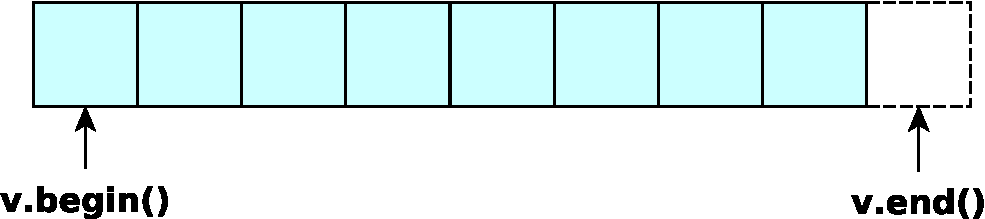
\includegraphics[width=1.0\textwidth]{illustrations/iter-starter-crop.pdf}
\caption{Первое представление об итераторах}
\label{fig:iter_starter}
\end{figure}

На (рис. \ref{fig:iter_starter}) показано, что \lstinline!v.end()! это специальный итератор за концом массива.

Пока что это всё, что нужно знать:
\begin{itemize}
\item Есть как минимум два способа получить итератор: методы \lstinline!begin()! и \lstinline!end()!
\item Итератор ведёт себя как указатель: его можно разыменовать или инкрементировать
\item Есть специальный ограничивающий итератор на конец контейнера.
\end{itemize}

Дерево из \ref{subsub:initializerlists} с помощью итераторов может быть заполнено из списка инциализации довольно просто.

\begin{lstlisting}
Tree(initializer_list<T> il) {
  for (auto it = il.begin(); it != il.end(); ++it)
    add_node(*it);
}
\end{lstlisting}


Дополнительная бонус-информация заключается в том, что большинство контейнеров поддерживают как метод \lstinline!assign!, принимающий диапазон итераторов и перекидывающая в контейнер содержимое этого диапазона, так и специальный конструктор из двух итераторов, который делает то же самое но при создании. Ниже показано использование этого конструктора для перекидывания списка инициализации в вектор.

\begin{lstlisting}
class Introw {
  vector<int> v_;
public:
  Introw(initializer_list<int> il) : v_(il.begin(), il.end()) {}
\end{lstlisting}

В целом, итераторы делают многие вещи проще и естественней. Разговор о них будет продолжен позже, а пока следует поговорить о контейнерах, для которых они нужны -- то есть таких, которые не поддерживают память одним куском и работу с ней через обычные указатели.

\subsection{Деки}\label{subsub:Deque}

Непрерывность памяти это очень строгая гарантия. На самом деле, последовательный контейнер может быть устроен так, чтобы не обязательно её давать -- например занимать произвольные участки памяти. Например это позволило бы сделать в таком контейнере эффективный \lstinline!push_front!, \lstinline!insert! или \lstinline!emplace! после любого элемента и так далее. Для таких целей, библиотека поддерживает односвязные списки (\lstinline!std::forward_list!), двусвязные списки (\lstinline!std::list!) и деки (\lstinline!std::deque!).

Дека (deque, от double ended queue, двусторонняя очередь, но созвучная также с английским словом deck -- колода карт) это почти магический контейнер, который поддерживает:

\begin{itemize}
\item Доступ к любому элементу за O(1) 
\item Вставку в начало и в конец за O(1) 
\item Вставку в произвольное место за O(n)
\end{itemize}

\textbf{Вопрос к студентам:} как бы вы организовали такой контейнер?

\ifanswers
Правильный ответ: последовательность кусков памяти фиксированного размера, связанных общей таблицей-заголовком
\fi

Самое главное в деке -- то, что она кусочно линейна и значит не требует резервирования памяти. Это тот самый контейнер, который \textbf{действительно} абстрагирует программиста от работы с памятью. Например следующий код уже встречался при разговоре о векторах

\begin{lstlisting}
deque<int> v;
for (int i = 0; i != N; ++i)
  v.push_back(i);
\end{lstlisting}

Но сейчас (и это кажется невероятным) с ним всё хорошо. Более того. Со следующим кодом, который для векторов был бы сущим безумием, тоже всё хорошо.

\begin{lstlisting}
deque<int> v;
for (int i = 0; i != N; ++i)
  v.push_front(i);
\end{lstlisting}

Здесь элементы добавляются в начало контейнера и это тоже происходит асимптотически быстро. Пожалуй единственный случай, когда программисту нужно думать о накладных расходах при работе с деками это накладные расходы на копирование тяжёлых объектов

\begin{lstlisting}
struct Heavy {
  explicit Heavy (int sz) {
    cout << "Heavy created" << endl;
  }

  Heavy(const Heavy &rhs) {
    cout << "Heavy copy-constructed" << endl;
  }

  Heavy (Heavy &&rhs) noexcept {
    cout << "Heavy move-constructed" << endl;
  }

  Heavy& operator= (const Heavy &rhs) {
    cout << "Heavy copied" << endl;
    return *this;
  }

  Heavy& operator= (Heavy &&rhs) noexcept {
    cout << "Heavy moved" << endl;
    return *this;
  }
};
\end{lstlisting}

Теперь становится прозрачным, что в случае использования \lstinline!push_front! для помещения таких объектов в деку:

\begin{lstlisting}
for (int i = 0; i != 5; ++i)
  d.push_front(Heavy(i));
\end{lstlisting}

Каждый из них должен быть не только создан, но и перемещён. А в случае использования \lstinline!emplace_front! -- только создан.

\begin{lstlisting}
for (int i = 0; i != 5; ++i)
  d.emplace_front(i);
\end{lstlisting}

Более подробно эта идея обсуждается в разделе про правые ссылки, так как существенно использует этот механизм (см. \ref{subsub:Emplace}).

Майерс \cite{effmoderncpp} рекомендует рассмотреть использование деки в качестве вашего основного контейнера.

\subsection{Списки}

Классический список это двусвязный \lstinline!std::list!, но начиная с C++11 добавлен также односвязный \lstinline!std::forward_list!, который тратит вдвое меньше ценной памяти на поддержку указателей (ценой отсутствия итерируемости назад).

В целом со списками можно делать то же самое, что и с векторами или деками: инициализировать, обращаться по итератору, добавлять и удалять элементы. Для добавления элементов в любое место служит у двусвязных списков метод \lstinline!insert!, который берёт итератор позиции сразу перед вставкой. Также удобно удалять элементы, это всегда происходит за O(1) и для этого есть специальный метод \lstinline!remove!

А вот переопределения квадратных скобок для списков не сделало, так как они бы внесли ненужную скрытую сложность. Увы, доступ к элементу по индексу в списке производится не менее чем за O(N).

Самой интересной возможностью у списков является \textbf{сплайс}\index{splice}. Это техника, позволяющая асимптотически быстро вынуть кусок из одного контейнера и вставить его в другой. Она проиллюстрирована на (рис. \ref{fig:list_splice}).

\begin{figure}[h!]
\centering
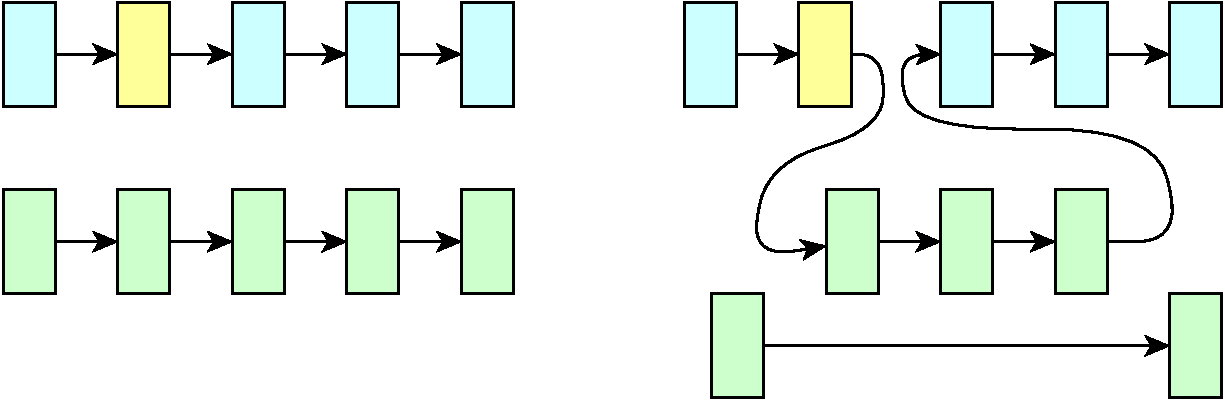
\includegraphics[width=1.0\textwidth]{illustrations/list-splice-crop.pdf}
\caption{Сплайс для односвязных списков}
\label{fig:list_splice}
\end{figure}

В качестве тренировки можно рассмотреть работу этой возможности. Первое, что надо сделать это подготовить сцену: обзавестись двумя списками

\begin{lstlisting}
forward_list<int> first = { 1, 2, 3 }; 
forward_list<int> second = { 10, 20, 30 }; 
auto it = first.begin(); // it -> 1
\end{lstlisting}

Тут видно как работает инициализация списком и взятие итератора на первый элемент. Теперь можно перекинуть весь второй список в первый. 

\begin{lstlisting}
first.splice_after (first.before_begin (), second);
\end{lstlisting}

Оп. Теперь второй список пуст, а первый содержит элементы 10, 20, 30, 1, 2, 3

При этом итератор it остался тем же и так же указывает на элемент 1! В разделе про итераторы будет подробнее рассмотрена эта цникальная особенность списков: итераторы остаются \textbf{валидными} при гораздо большем спектре операций над списком, подробнее см. (\ref{subsub:valinval}).

Далее можно, например, перкинуть элементы со второго по it в список second

\begin{lstlisting}
second.splice_after (second.before_begin(), first, first.begin(), it);
\end{lstlisting}

Снова магия. Теперь первый список содержит 10, 1, 2, 3, а второй 20, 30

\textbf{Вопрос к студентам:} как теперь перекинуть все элементы второго списка начиная со второго (то есть в данном случае только 30) в первый список?

\ifanswers
С тем, что уже известно, это не так уж и сложно.

\begin{lstlisting}
first.splice_after (first.before_begin(), second, second.begin());
\end{lstlisting}
\fi

Тренироваться со сплайсом забавно, но у стандартных списков есть и тёмные стороны. Например они требуют некоторой аккуратности при необходимости вычислить размер.

\begin{lstlisting}
template <typename Container> 
void foo (Container &c) 
{
  if (c.size() == 0)
    {
      // processing
    }
  // processing
}
\end{lstlisting}

Этот обобщённый код выглядит хорошим только пока не предположить, что он должен работать со списками. В этом случае \lstinline!size! работает не за константное, а за линейное время.

К счастью, все стандартные контейнеры поддерживают функцию \lstinline!empty()!, выполняющуюуся за константное время. Поэтому правильная версия вышеприведённого фрагмента кода будет выглядеть как-то так.

\begin{lstlisting}
if (c.empty())
  // processing
\end{lstlisting}

И тут может возникнуть закономерный вопрос: но почему это так? Казалось бы, размер вполне можно было хранить как атрибут и отдавать за O(1).

Увы, здесь есть чисто инженерный баланс: если размер хранится как атрибут, то операция \lstinline!splice! должна его обновлять, а для этого пересчитывать элементы которые она удаляет и вставляет. Но это сделает сложность \lstinline!splice! линейной. Таким образом выбор стоит так: из пары методов \lstinline!size! и \lstinline!splice! для списков один любой может быть O(1), но никогда не оба.

\textbf{Вопрос к студентам:} можете ли вы себе представить двусвязный список, который делает reverse за константное время? Чем придётся заплатить?

\ifanswers
Например хранить в списке поле direction и сверяться с ним при переходе к next для выбора конкретной связи для перехода. Цена в общем-то невелика, но обычно её не платят, уж больно reverse специфичная и редко нужная штука.
\fi

\subsection{Адаптеры}

Некоторые распространённые ``контейнеры'', такие как стек или очередь, на самом деле не являются контейнерами в смысле стандартной библиотеки, поскольку не определяют внутреннего представления своих данных. Что мы подразумеваем, говоря ``стек''? Всего лишь набор операций, позволяющий снять элемент, положить элемент, посмотреть последний элемент. Такой набор операций может работать и для вектора и для деки и для списка. Поэтому в стандартной библиотеке, стеки и очереди реализованы не как контейнеры, а как \textbf{адаптеры} контейнеров.

\begin{figure}[ht]
\centering
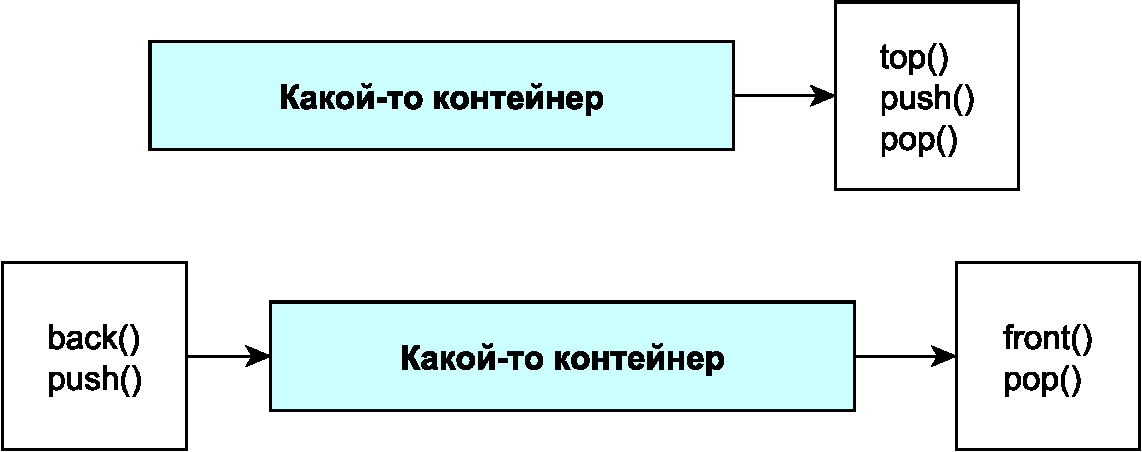
\includegraphics[width=0.9\textwidth]{illustrations/adapters-crop.pdf}
\caption{Адаптеры стека и очереди}
\label{fig:adapters_sq}
\end{figure}

На (рис. \ref{fig:adapters_sq}) показаны адаптеры стека и очереди. Контейнеры под ними в принципе произвольные, но стандарт даёт разумные умолчания.

Всего в стандартной библиотеке сейчас определены три вида адаптеров:

\begin{enumerate}
\item \textbf{stack} – LIFO стек над последовательным контейнером
\begin{lstlisting}
template <class T, class Container = deque<T> > 
class stack;
\end{lstlisting}
\item \textbf{queue} – FIFO очередь над последовательным контейнером
\begin{lstlisting}
template <class T, class Container = deque<T> > 
class queue;
\end{lstlisting}
\item \textbf{priority\_queue} – очередь с приоритетами (как binary heap) над последовательным контейнером
\begin{lstlisting}
template <class T, 
          class Container = vector<T>,
          class Compare = less<typename Container::value_type>>
class priority_queue;
\end{lstlisting}
\end{enumerate}

К сожалению адаптеры не слишком ортогональны: они берут одновременно и класс и тип, которым он параметризован. Это даёт неограниченные возможности выстрелить себе в ногу.

\begin{lstlisting}
stack <int> s; // ok, stack <int, deque<int>>
stack <int, vector<long>> s1; // bad
stack <int, vector<char>> s2; // really bad
s2.push(1000);
\end{lstlisting}

\textbf{Вопрос к студентам:} что реально будет помещено в стек s2?

\ifanswers
Правильный ответ: 256 - (1024 - 1000) это 232.
\fi

Казалось бы логично использовать шаблонные шаблонные параметры. Простейшая попытка такого рода может быть проиллюстрирована ниже

\begin{lstlisting}
template <class T, 
          template <class T> class Container = deque> 
class stack;
\end{lstlisting}

Казалось бы такой адаптер уже нельзя использовать неправильно.

\begin{lstlisting}
stack<int, vector> s;
\end{lstlisting}

\textbf{Вопрос к студентам:} почему эта система не будет работать?

\ifanswers
Правильный ответ: потому что у вектора не один шаблонный параметр
\fi

Кроме того, некоторые контейнеры просто не являются подходящими. Хуже всего, что никакой статической проверки не предусмотрено и неподходящесь контейнера часто выясняется внезапно.

\begin{lstlisting}
stack <int, forward_list<int>> s; // ok
\end{lstlisting}

Эта строчка превосходно скомпилируется, но попытка использовать любой метод из интерфейса будет провалена.

\begin{lstlisting}
s.push(100); // fail: no push_back
s.pop(); // fail: no pop_back
s.top(); // fail: no back
\end{lstlisting}

Эти ошибки неочевидны. Стек вполне может быть сделан на односвязном списке.

\textbf{Вопрос к студентам:} вы понимаете как сделать стек на односвязном списке?

\ifanswers
Правильный ответ: добавлять в голову и удалять с головы.
\fi

Но увы, адаптер \lstinline!std::stack! требует (неявно требует) вполне определённый интерфейс.

\subsection{Контейнеро-подобные классы}

В этом разделе речь пойдёт об удобных контейнеро-подобных классах, не являющихся, тем не менее, полноценными контейнерами. Начать стоит с мотивирующего примера.

Очень часто люди, привычные к математической нотации вектора неудоумевают почему в С++ оператор сложения для векторов не работает в математическом смысле.

Например, всегда есть соблазн определить

\begin{lstlisting}
vector<int> v1 = {1, 2, 3, 4};
vector<int> v2 = {10, 20, 30, 40};
assert(v1 + v2 == vector<int>{11, 22, 33, 44});
\end{lstlisting}

Например так можно было бы сделать, создав отдельную специализацию vector для типов, похожих на интегральные.

\textbf{Вопрос к студентам:} почему так делать нельзя?

\ifanswers
Правильный ответ: к этому моменту \lstinline!vector<bool>! уже должен был кое-чему нас научить. Каждая специализация такого рода внутри стандартной библиотеки это потенциальная проблема для использования вектора в обобщённом контексте.
\fi

Вместо этого в стандарт включен специальный класс \lstinline!valarray!. У этого класса сложная судьба: будучи введён для математических вычислений, он, с развитием метапрограммирования, был практически вытеснен такими библиотеками как Eigen, основанными на шаблонах.

Тем не менее, в него было заложено несколько крайне интересных концепций, в том числе серьёзно упрощающих векторизацию операций над ним, и вполне достойных отдельного рассмотрения.

Во-первых, конечно, valarray ведёт себя именно как вектор при сложении.

\begin{lstlisting}
valarray<int> v1 = {1, 2, 3, 4};
valarray<int> v2 = {10, 20, 30, 40};
assert(v1 + v2 == valarray<int>{11, 22, 33, 44});
\end{lstlisting}

И даже умножение у него поэлементное

\begin{lstlisting}
valarray<int> v4 = v1 * v2 + v1 + v2; // { 62, 123, 305, 567 }
valarray<int> v4 = pow (v1, 2); // 4, 9, 25, 49
\end{lstlisting}

Но настоящая мощь valarray в том, что для него существуют векторные указатели (slices\index{slice}).

\begin{lstlisting}
valarray<int> row(n);
slice red(0, n/3, 3);
row[red] = 255; 
\end{lstlisting}

Этот код установит каждую третью ячейку row в значение 255.
Векторный указатель slice имеет начало, конец и инкремент, он похож на запись цикла и действительно можно было бы записать (но слайс эффективней):

\begin{lstlisting}
for (int i = 0; i != n; i += 3)
  row[i] = 255;
\end{lstlisting}

Вторым важным контейнеро-подобным классом является жалкая попытка комитета отыграться за \lstinline!vector<bool>!, а именно битовая маска \lstinline!std::bitset!

На самом деле, конечно, \lstinline!bitset! это альтернатива \lstinline!array<bool>! то есть у него фиксированный размер, являющийся параметром контейнера. При этом он хранит данные более компактно (тоже суббайтно, как и \lstinline!vector<bool>!).

\begin{lstlisting}
// 24-bit number
bitset<24> s1 = 0x7ff000;
bitset<24> s2 = 0xff00;
s1[0] = 1; // either s1.set(0) or s1.set(0, 1)
auto s3 = s1 & s2; // s3 = 0xf000
\end{lstlisting}

Вообще хранение чего угодно ниже минимально адресуемого адресного пространства выглядит в трансляционной модели языка странно и, по идее, должно приводить к проблемам. Но в данном случае речь о хорошо изученном механизме, относительно которого накоплен определённый опыт.

Конечно очень не хватает для битовых масок слайса, но слайса нет и для обычной битовой арифметики.

TODO: неудавшийся \lstinline!array_view! и грядущий \lstinline!span!

\pagebreak
\section{Ввод и вывод}\label{subsec:iostreams}

\hfill\textit{From a programmer's point of view,}

\hfill\textit{the user is a peripheral}

\hfill\textit{that types when you issue a read request}{\vspace{0.5em}}

\hfill\textit{-- Peter Williams} 

Что-то про ввод и вывод уже было сказано в (\ref{PrintfToCout}), здесь базовые вещи будут считаться уже понятными, но многое сознательно будет изложено повторно. 

Ввод и вывод это самая старая часть нынешней стандартной библиотеки C++ и единственная её часть, которая действительно широко использовалась до стандартизации языка. Причём, эта подсистема действительно странная штука. Пусть необходимо просто распечатать целое число в 16-ричном формате. Как к этому подходят разные языки:

\begin{itemize}
\item \textbf{C } -- \lstinline!fprintf(stdout, "%x", n)!
\item \textbf{Python} -- \lstinline!print("%x" % n)!
\item \textbf{Java} -- \lstinline!System.out.println(String.format("%x", n))!
\item \textbf{Perl} -- \lstinline!printf "%d\n", n!
\item \textbf{C\#} -- \lstinline!Console.WriteLine("{0:x}", n);!
\item \textbf{Rust} -- \lstinline?println!("{0:x}", n)?
\item \textbf{Go} -- \lstinline!fmt.Printf("%x", n)!
\end{itemize}

А теперь внимание, как это выглядит на C++

\begin{lstlisting}
std::cout << std::hex << n;
\end{lstlisting}

Причем многие языки из перечисленных выше, были, на самом деле, созданы гораздо позже C++. Это наводит на мысли о том, так ли удачна была разработанная в свое время для C++ система вывода, если все новые языки с криком разбегаются от неё, предпочитая копировать сишную с разными улучшениями? Но то, что застыло в истории языка, застыло там навсегда. Странная система стандартного ввода-вывода в C++ имеет место, она не всегда может быть заменена старыми добрыми сишными возможностями, ей часто (и обоснованно) пользуются и её лучше знать, чем не знать.

\subsection{Проблемы с C-style IO}

С точки зрения программиста на C++, C-style IO, хотя и доступен в языке, но имеет массу проблем. Вот только некоторые:

\begin{itemize}
\item Нерасширяемость. Например как определить новый форматный спецификатор?
\item Неочевидность: выбор спецификатора определяется размером, который может не быть известен. Пример: \lstinline!int64_t! требует препроцессора для крайне ``читаемого'' вывода в стиле: \lstinline!printf("x = %"PRIu64"d", x)!
\item Небезопасность относительно типов: \lstinline!printf("%s\n", 1)! не просто скомпилируется, а ещё и исполнится, приведя при этом к таким проблемам, которые вы поседеете искать и отлаживать.
\item Небезопасность относительно количества аргументов.
\item Нерасширяемость самого механизма файловых дескрипторов (ограниченных \lstinline!FILE*!).
\end{itemize}

Чтобы решить все эти проблемы, язык C++ вводит несколько уровней абстракции: главным объектом связывающим воедино ввод и вывод становятся не файлы, а \textbf{потоки}, которые отдают техническую реализацию ввода и вывода своим буферным классам, а форматирование своим локалям с присущим им фасетами. Сами же они занимаются тем, что предоставляют ко всему этому сложный интерфейс, построенный во многом на переопределении операторов и прочих уникальных языковых возможностях.

При разговоре о переопределении операторов была высказана дельная мысль о том, что стоит избегать семантически безумных определений. Например плохая идея переопределять \lstinline!operator *! для произведения матриц, так как оно не коммутативно и т.д. Обо всем этом на время чтения этого раздела стоит забыть: большего безумия, чем переопределить битовый сдвиг для ввода и вывода и представить себе невозможно. С этим нужно смириться.

Кроме того, потоки ввода/вывода (streams) не следует путать с потоками исполнения (threads), это очень разные вещи. Это настолько разные вещи, что я даже убрал слово ``потоки'' из заголовка раздела, чтобы не вводить в искушение во-первых и потому что оно уже есть в названии раздела про потоки исполнения во-вторых.

\subsection{Иерархия классов для IO}

Хорошим тоном в литературе считается сразу вдохновлять читателей иллюстрацией иерархии потоков ввода-вывода.

TODO: тут картинка

Несмотря на запутанность общей картины, глаз сразу выделяет основные паттерны. Есть две независимых иерархии для буферов с корнем в \lstinline!basic_streambuf! и для потоков с корнем в \lstinline!basic_ios! (который агрегирует \lstinline!basic_streambuf!, поскольку каждый поток владеет своим буфером). Иерархия потоков отчетливо ветвится на ввод и вывод, а потом ромбовидно сходится на \lstinline!basic_iostream!, от которого наследуют гибриды.

Вся эта иерархия это не столько иерархия классов, сколько иерархия шаблонов. Собственно классы, такие как \lstinline!ostream! или \lstinline!fstream! инстанцируют соответствующие шаблоны, определяя тип символов, который будет в них выводиться. Типы символов бывают разные, но об этом позже, а пока представим, что \lstinline!char! хватает для всех.

\subsection{Форматирование}\label{FormattedIO}

Как ни странно, форматированный ввод и вывод оказывается гораздо проще неформатированного.

\begin{lstlisting}
int n = 42;
cout << n << endl; // 42
cout << hex << n << endl; // 2A
\end{lstlisting}

Форматный модификатор меняет состояние потока, поэтому вовзратится от шестнадцатиричного вывода к десятичному, нужно явно.

\begin{lstlisting}
cout << hex << n << " " << dec << n << endl; // 2A 42
\end{lstlisting}

Аналогично ввод. Можно поиграть с простой программой, которая ждёт 16-ричное число и переводит его в десятичное.

\begin{lstlisting}
int n;
cin >> std::hex >> n;
cout << std::dec << n << std::endl;
\end{lstlisting}

Например если ввести 2A и нажать ввод, программа выведет 42 и завершит работу.

\textbf{Вопрос к студентам:} а что будет если ввести нечто странное, вроде AAAAAAAAAAAAAAAAAAAAAA?

\ifanswers
Будет поведение, зависящее от реализации. Как вариант вывод MAXINT, то есть чего-то вроде 2147483647.
\fi

Полный список стандартных манипуляторов всегда можно посмотреть в стандарте (вариант для слабаков -- нагуглить в интернетах). В основном они разделяются на:

\begin{itemize}
\item Форматные модификаторы такие как \lstinline!hex! и \lstinline!dec! для целых или \lstinline!fixed! и \lstinline!scientific! для чисел с плавающей точкой.

\item Специальные манипуляторы, такие как \lstinline!endl! или \lstinline!ends!

\item Независимые флаги: \lstinline!skipws!, \lstinline!showpos!, \lstinline!uppercase!, \lstinline!boolalpha! и т.д. Обычно они все имеют отрицательные пары: \lstinline!noskipws!, \lstinline!noshowpos! и так далее

Например в приведенной выше программе, ввод ``  2A'' будет засчитан как 42, потому что пробелы не учитываются по умолчанию. Но это можно изменить:

\begin{lstlisting}
cin >> std::hex >> std::noskipws >> n;
\end{lstlisting}

Теперь ввод лишних пробелов будет ошибкой.

\item Параметризованные манипуляторы, такие как \lstinline!setfill! или \lstinline!setbase!, которые принимают дополнительные аргументы.

Вот так, например, можно вывести число в поле ширины 10, заполненное точками в пустых местах.

\begin{lstlisting}
cout << std::setfill ('.') << std::setw (10) << 42;
\end{lstlisting}

В результате получится \lstinline!........42!. Точек восемь а не десять, потому что 10 это общая ширина поля для вывода.

\end{itemize}

Важно понимать, что все манипуляторы это просто функции, поэтому кроме использования перегруженных операторов сдвига, можно просто вызывать эти функции с потоком в качестве аргумента.

\begin{lstlisting}
cout << hex; // operator << (cout, hex)
             // calls hex(cout);
hex(cout);   // call immediately
\end{lstlisting}

Обе записи равноправны, но первая бывает более удобна, когда в одной цепочке надо часто переключать манипуляторы.

Манипуляторы бывают очень простыми. Например манипулятор \lstinline!endl! может быть устроен как-то так:

\begin{lstlisting}
template <typename charT, typename traits>
std::basic_ostream<charT,traits>&
std::endl (std::basic_ostream<charT,traits>& strm)
{
  strm.put(strm.widen(’\n’));
  strm.flush();
  return strm;
}
\end{lstlisting}

Пока что тут непонятна функция \lstinline!widen!, но интуитивно ясно, что она приводит символ конца строки к правильному формату конца строки в потоке, который может быть параметризован иным типом символов. Такие манипуляторы вполне можно писать самому. Но эта относительная простота обманчива: она сохраняется лишь пока нет необходимости работать с состоянием потока. Как ни странно, но разговор о написании собственного манипулятора, работающего с этим состоянием (как это делает, например \lstinline!std::hex!, придётся отложить до рассмотрения локалей и фасетов (см. \ref{Localization}).

И того, что операторы ввода и вывода это перегруженные операторы логического сдвига, следует, что их можно переопределять для любого класса

\begin{lstlisting}
class MyClass
{
  //  something private
public:
  // print have access to private data
  void print (std::ostream& stream) const; 
}

std::ostream& operator <<(std::ostream& stream, const MyClass& rhs) 
{
  rhs.print (stream);
  return stream;
}
\end{lstlisting}

Многие любят использовать для операторов вывода дружбу. Дело вкуса, но мне кажется, не стоит лишний раз давить кишки наружу, нарушая инкапсуляцию класса.

\subsection{Неформатный ввод и вывод}

Ввод без форматирования позволяет снова разделить ответственности: теперь потоки ввода оказываются нужны только для чтения (например посимвольного или построчного), а весь разбор программа берет на себя. Обычная ситуация в мире C++ это сочетания неформатированного ввода с форматированным выводом, потому что в форматированном вводе куда как сложнее обрабатывать ошибки.

Основные средства для посимвольного чтения из потока: 

\begin{itemize}
\item \lstinline!get! -- считывает из потока один символ 
\item \lstinline!peek! -- подсматривает в потоке один символ 
\item \lstinline!putback! -- кладёт считанный символ обратно в поток. Стандартом гарантируется возможность положить обратно один только что считанный символ, но реализации иногда позволяют больше.
\end{itemize}

Можно поиграть со следующим кодом.

\begin{lstlisting}
char c = cin.get();
if ( (c >= '0') && (c <= '9') ) 
{
  int n;
  cin.putback (c);
  cin >> n;
  // process number
} 
else 
{
  string str;
  cin.putback (c);
  getline (cin, str); // not cin.getline (char *, int)
  // process string
}
\end{lstlisting}

\textbf{Вопрос к студентам:} можно ли использовать \lstinline!peek!, чтобы переписать его чуть лучше?

\ifanswers
Правильный ответ:  да, конечно, тогда и \lstinline!putback! можно убрать.
\fi

Особое внимание нужно обратить на \lstinline!getline! из заголовочника \lstinline!<string>!. Дело в том, что у потока ввода есть свой \lstinline!getline! но он был спроектирован раньше, чем \lstinline!string! и не умеет динамически увеличивать буфер, а требует заранее заданного размера.

Особенности ввода иногда порождают сложные и трудно отлавливаемые проблемы.

\begin{lstlisting}
cout << "Please enter a number: " << "\n";
cin >> num;
cout << "Your number is: " << num << "\n";
cout << "Please enter your name: \n";
getline (cin, mystr);
\end{lstlisting}

Эта программа кажется совершенно правильной... вот только она не считывает имя пользователя.

\textbf{Вопрос к студентам:} как вы думаете в чем дело?

\ifanswers
Правильный ответ: см. ниже.
\fi

Дело в том, что после ввода числа, в потоке ввода ``залип'' перевод строки. Для того, чтобы его оттуда убрать, используется метод \lstinline!ignore!

\begin{lstlisting}
cout << "Please enter a number: " << "\n";
cin >> num;
cout << "Your number is: " << num << "\n";
cout << "Please enter your name: \n";
cin.ignore();
getline (cin, mystr);
\end{lstlisting}

На самом деле этот метод имеет параметры: сколько символов проигнорировать и на каком остановиться, но чаще всего он вызывается именно так для игнорирования одного символа (обычно возврата строки).

\subsection{Состояния и обработка ошибок}

Каждый поток ввода/вывода находится в том или ином состоянии после каждой операции. Обычно для потоков вывода это не слишком критично, так как сложно представить себе ошибку вывода (впрочем при выводе в файл или строку они бывают). Поэтому в 99 процентах случаев проверка состояний используется для потоков ввода.

Состояние задаётся тремя битами: \lstinline!eofbit!, \lstinline!failbit! и \lstinline!badbit!. Если ни один из этих битов не установлен, состояние считается хорошим (иногда используется термин \lstinline!goodbit!, но автору он не нравится, так как нет такого бита). Различия между тремя плохими состояниями довольно просты:

\begin{itemize}
\item \lstinline!std::ios_base::eofbit! -- считан конец файла (EOF можно проэмулировать с клавиатуры, в unix-системах это Ctrl-D)
\item \lstinline!std::ios_base::failbit! -- восстановимая ошибка. Например ошибка форматирования, когда ожидается число, а считана строка
\item \lstinline!std::ios_base::badbit! -- серьёзная ошибка: поток испорчен или информация потеряна. Например позиционирование потока раньше начала файла, etc.
\end{itemize}

Обычно \lstinline!eofbit! и \lstinline!failbit! случаются вместе, так как почти ни один файл в нашем мире не завершается символом конца файла, вместо этого конец файла детектируется при неудачной попытке считать после конца файла.

Также в \lstinline!std::ios_base! поддерживается функция \lstinline!rdstate! позволяющая считать флаги и функция \lstinline!clear!, позволяющая их сбросить. Особое место занимает функция \lstinline!fail!, которая возвращает \lstinline!true!, если установлен \lstinline!failbit! \textbf{или} \lstinline!badbit!.

Для потоков также переопределены два оператора: неявное преобразование \lstinline!operator bool()! соответствует \lstinline?!fail()? и оператор отрицания (о нет, опять) \lstinline?operator !()?, соответствующий \lstinline?fail()?.

Можно попробовать программу:

\begin{lstlisting}
int n;

while (cin >> n)
{
  cout << n << endl;
  cin.ignore(); // eating Enter hit
}
\end{lstlisting}

\textbf{Вопрос к студентам:} что она выведет если вы введете 1.1?

\ifanswers
Правильный ответ: она выведет
\begin{verbatim}
1 
1
\end{verbatim}
так как точка будет съедена в ignore.
\fi

С этой проверкой с неявным преобразованием связана глупая ошибка. Люди пишут:

\begin{lstlisting}
if (!cin >> n)
{
  // process errors
}
\end{lstlisting}

Что при этом случается: сначала вызывается \lstinline?operator !()?, который возвращает текущее состояние потока, а потом оно приводится к целому и сдвигается вправо на n. Наверное это не то, чего вы хотели. То, что вы хотели, достигается расстановкой скобок.

\begin{lstlisting}
if (!(cin >> n))
{
  // process errors
}
\end{lstlisting}

Но на самом деле, то, чего вы хотели достигается тем, что вы прекращаете выпендриваться и пишете прозрачный и читаемый код:

\begin{lstlisting}
cin >> x;
if (cin.fail()) {
  // process errors
}
\end{lstlisting}

Интересно, что из-за почтенного возраста библиотеки, вся обработка ошибок производится без использования исключений и это идёт скорее на пользу: ошибка пользовательского ввода это почти никогда не исключительная ситуация. Механизмы завести ошибки потоков на исключения есть, но я о них рассказывать не буду, чтобы не навредить.

\subsection{Работа с файлами}

Настоящая мощь потоков раскрывается через прозрачную работу с файлами. Главное преимущество это RAII (см. \ref{RAII}) выражающееся в том, что файлы живут под потоками, открываются и закрываются по необходимости. Всё, что нужно в простейшем случае, это имя файла и иногда режим в котором его открыть.

Первый пример из \cite{josuttis2}: записать текущий charset в файл

\begin{lstlisting}
{
  ofstream file(filename);

  if (! file) 
    {
      // process errors
    }

  // write character set
  for (int i = 32; i < 256; ++i) 
    {
      file << "value: " << setw(3) << i << " " 
           << "char: " << static_cast<char>(i) << endl;
    }

} // scope ends
\end{lstlisting}

Файл будет автоматически закрыт в конце своей области видимости.

Второй пример: выдать содержимое файла на экран:

\begin{lstlisting}
ifstream file(filename);

// check for errors like above

char c;
while (file.get(c)) 
  cout.put(c);
\end{lstlisting}

Это сразу вызывает вопрос: а что если файл нужен мне дольше, чем его область видимости? Раньше в C++98 это приводило к уродливым хакам, вроде создания потока в динамической памяти. Но в C++11 для файлов определен move ctor и следующий код становится легальным:

\begin{lstlisting}
std::ofstream 
openFile (const std::string& filename)
{
  std::ofstream file(filename);
  file << "hello, ";
  return file;
}

std::ofstream file;
file = openFile("xyz.tmp");
file << "world" << std::endl;
\end{lstlisting}

Возможен и обратный вопрос: можно ли один поток использовать для нескольких файлов? И снова ответ положительный: для этого используются функции \lstinline!open! и \lstinline!close!, позволяющие закрыть нижележащий файл и заново его открыть.

Файлы могут быть открыты с тонким управлением режимами. Например если записанный внутри функции файл был там закрыт, его можно открыть на дозапись (append) скомбинировав флаги вручную.

\begin{lstlisting}
ofstream file("a.tmp", std::ios_base::out|std::ios_base::app);
\end{lstlisting}

Полный список флагов несложно посмотреть в стандарте. Гораздо полезнее знать их соответствие распространённым флагам из мира C.

\begin{center}
\begin{tabular}{ | l | l | l | }
  \hline
  Тип & Файл & Поток \\ \hline
  Чтение & \lstinline!"r"! & \lstinline!in! \\
  Перезапись & \lstinline!"w"! & \lstinline!out! или \lstinline!out|trunc! \\
  Дозапись & \lstinline!"a"! или \lstinline!"a+"! & \lstinline!app! или \lstinline!in|out|app! \\
  Чтение/запись с начала & \lstinline!"r+"! & \lstinline!in|out! \\
  Чтение/перезапись & \lstinline!"w+"! & \lstinline!in|out|trunc! \\
  \hline
\end{tabular}
\end{center}

Файловые потоки вывода при записи можно позиционировать

\begin{lstlisting}
outfile << "This is an apple";
long pos = outfile.tellp();
outfile.seekp(pos - 7);
outfile << " sam";
\end{lstlisting}

\textbf{Вопрос к студентам:} что окажется в файле?

\ifanswers
Правильный ответ: this is a sample
\fi

Приведенный выше код обычно работает, но после 2011 года хорошим тоном считается не закладываться на то, что результат \lstinline!tellp! можно преобразовать к \lstinline!long! и обратно. Более правильным будет написать:

\begin{lstlisting}
  auto pos = outfile.tellp();
  outfile.seekp (pos - static_cast<decltype(pos)>(7));
\end{lstlisting}

Это чуть дольше, но это уберегает от неприятностей при поддержке кода.

Ещё лучше сформулировать относительный поиск как относительный. Если всё что нужно это перебазировать на семь позиций от текущей позиции, то сработает следующий подход.

\begin{lstlisting}
outfile << "This is an apple";
outfile.seekp (-7, std::ios::cur);
outfile << " sam";
\end{lstlisting}

Он, пожалуй, и является в этом случае оптимальным. Разумеется, наравне с \lstinline!cur! доступна относительная привязка к \lstinline!beg! и \lstinline!end!.

Не все потоки поддерживают позиционирование, например его по понятным причинам не поддерживают \lstinline!cin! и \lstinline!cout!.

\subsection{Бинарный ввод и вывод}

Файлы бывают не только текстовые. 

TODO: тут про бинарный ввод и вывод.

\subsection{Работа со строками}\label{subsub:strstream}

Строка является удивительным объектом для ввода и вывода -- по сути она не связана ни с какой аппаратурой, а являет собой просто буфер в памяти с приятным интерфейсом доступа и форматирования.

Строковые потоки могут быть созданы как независимо, так и из строк. Пример должен быть уже понятен.

\begin{lstlisting}
std::ostringstream fst;
int n;
float f;

fst << 42.2442;
std::string s1 = fst.str();
std::istringstream iss(s1);
iss >> n >> f;
std::string s2("value: ");
std::ostringstream snd (s2, std::ios::out|std::ios::ate);
snd << std::hex << n << " " << f;
std::cout << snd.str() << std::endl;
\end{lstlisting}

Сначала в пустой и чистый строковый поток выводится значение числа с плавающей точкой. Потом его результат извлекается в строку. Далее из этой строки создаётся поток ввода и из него извлекается целое и число с плавающей точкой. Далее создаётся строка с текстом, потом из неё поток и в этот поток извлеченное целое выводится в шестнадцатеричном виде. И наконец, всё это оказывается на экране.

\textbf{Вопрос к студентам:} что окажется на экране?

\ifanswers
Правильный ответ: value: 2a 0.2442
\fi

Строковые потоки даже не обязаны быть именованными (код ниже требует C++11).

\begin{lstlisting}
void parseName(string name)
{
  string s1, s2, s3;
  istringstream(name) >> s1 >> s2 >> s3;
  .....
\end{lstlisting}

Разумеется, как и файловые потоки они поддерживают и семантику перемещения и позиционирование.

Ранее (см. \ref{subsub:stringview}) была рассмотрена гипотетическая функция combine.

TODO: тут комбинатор на вариабельных шаблонах

\subsection{Буферизация}

Как и было сказано (см. \ref{PrintfToCout}), с каждым потоком связан буфер (возможно нулевого размера). При этом буферизация бывает построчная полная или никакая. Средства C++ тоже позволяют управлять буферизацией.

Уже несколько раз был упомянут прямой вывод содержимого любого потока на экран

\begin{lstlisting}
char c;
while (file.get(c)) 
  cout.put(c);
\end{lstlisting}

Если ещё раз вернуться к коду выше, то он очевидно неоптимален. Оптимальный метод выглядит даже проще:

\begin{lstlisting}
cout << file.rdbuf();
\end{lstlisting}

Странная функция \lstinline!rdbuf! имеет два предназначения: без аргументов она возвращает указатель на буфер потока, с аргументом она устанавливает буфер. Например дебуферизовать стандартный ввод можно очень легко.

\begin{lstlisting}
cout.rdbuf(nullptr);
\end{lstlisting}

Но обычная задача это как раз наоборот: задать буфер побольше для файлового потока, чтобы минимизировать количество чтений с диска и записей на диск.

Разумеется, для буферизованных потоков нужно не забывать сбрасывать их содержимое из буфера на устройство и делать это приходится руками. Тем не менее, есть некоторые иные механизмы для распространенных случаев. Например, кажется, что этот код не должен ничего печатать на экран до ввода:

\begin{lstlisting}
std::cout << "Please enter x: ";
std::cin >> x;
\end{lstlisting}

Но он печатает. Это происходит по двум причинам:

\begin{enumerate}
\item стандартный ввод в C++ связан (tied) со стандартным выводом
\item стандартный вывод cout в C++ синхронизирован (имеет один буфер) со старым добрым stdout
\end{enumerate}

Если развязать обе эти связи, то поведение кода становится ожидаемым:

\begin{lstlisting}
std::cin.tie (NULL);
std::cout.sync_with_stdio(false);
std::cout << "Please enter x: ";
std::cin >> x;
\end{lstlisting}

Функция \lstinline!tie! связывает потоки отношением ``случается до''. То есть заставляет все побочные эффекты одного потока случится до начала работы с другим. Но можно связать потоки ещё крепче, заставив их физически использовать один буфер:

\begin{lstlisting}
ostream hexout(std::cout.rdbuf());
hexout.setf (std::ios::hex, std::ios::basefield);
hexout.setf (std::ios::showbase);

std::cout << 42 << " ";
hexout << 42 << std::endl;
\end{lstlisting}

На экране будет: ``42 0x2a''. Это вывод в один и тот же стандартный вывод, только теперь он по-разному форматирован.

\textbf{Домашняя наработка:} почему вывод указателя на буфер потока ввода выводит в поток вывода не указатель, а всё, что вводится в поток ввода?

\pagebreak
\section{Локализация}\label{Localization}

Не все буквы можно поместить в диапазон однобайтных символов. Пока речь идёт только об английском языке, всё неплохо, но русские буквы, европейская диакритика, и даже иероглифическое письмо также имеют свое место в мире C++.

В доисторические времена считалось, что английских символов хватит на всех. Из этих времён до нас дожил стандарт ANSI, предполагающий 7-битные кодировки. Его расширение ASCII предлагало 8 бит, первые 128 символов совпадали с ANSI, а оставшиеся 128 определялись \textbf{кодовой страницей}. В качестве примера всем известны CP-1251 и CP-866.

Тогда же возникли многословные (multibyte) строки и форматы. Например если зафиксировать байт 0x90 для специального случая (следующий символ означает нечто иное), то можно получить 511 символов вместо 256. Люди фиксировали целые диапазоны и как-то крутились. Проблема в том, что в такой кодировке очень сложно работать таким функциям как strcmp или strlen.

Система Unicode предлагает отличие между системой кодировки (Universal Character Set, UCS) и форматом преобразования (Universal Translation Format, UTF). 

Основные системы кодировки это UCS-2, кодирующая символы по 16 бит и UCS-4, кодирующая по 32 бита. С последней возможны широкие (wide) кодировки, когда каждый символ занимает по 4 байта и этого хватает на всех. Но до сих пор самые частые символы это старые добрые символы из ANSI, которые можно кодировать одним байтом.

Поэтому трансляции поддерживаются следующие:

\begin{enumerate}
\item UTF-8 (от 1 до 6 байт на символ) в ней U+0410 это {0xD0, 0x90}, зато U+0041 это {0x41}
\item UTF-16 (покрывает UCS-2) в UTF16-LE U+0410 это {0x10, 0x04} но и U+0041 это {0x41, 0x00}
\item UTF-32 (покрывает UCS-4)
\end{enumerate}

Цель этого раздела показать как эти возможности ложаться на язык и к чему это приводит.

В английском языке слово ``интернационализация'' (internationalization) весьма длинное с точки зрения носителей языка, поэтому оно часто сокращается до ``i18n''. Также в литературе используется ``l10n'' для ``локализации'' (localization).

\subsection{Символы и характеристики символов}

Стандарт определяет четыре основных типа для представления символов:

\begin{itemize}
\item \textbf{char} -- тип минимального размера. \lstinline!sizeof(char) == 1!
\item \textbf{char16\_t} -- символьный тип для UCS-2
\item \textbf{char32\_t} -- символьный тип для UCS-4
\item \textbf{wchar\_t} -- наиболее широкий символьный тип из всех, присутствующих в системе
\end{itemize}

Обычно символьный тип является главным параметром шаблона для таких классов, как строки, потоки и им подобных. Например общий шаблон потока

\begin{lstlisting}
template <typename charT, typename traits = char_traits<charT>>
class basic_istream;
\end{lstlisting}

Далее определяется для разных типов символов в разные синонимы.

\begin{lstlisting}
typedef basic_istream<char> istream;
typedef basic_istream<wchar_t> wistream;
\end{lstlisting}

Гораздо более интересен второй аргумент, который идёт по умолчанию: характеристики символов. Одни и те же по ширине символы могут подчиняться разным правилам сравнения, копирования, иметь разный размерный тип и даже разное представление EOF (подробнее см. \ref{subsub:strtraits}).

По умолчанию характеристики определены для каждого из стандартно поддержанных символов, но никто не ограничивает в том, чтобы определить и передать свои.

\subsection{Локали}\label{subsubsec:locales}

Локали инкапсулируют национальные и культурные конвенции. Самый простой способ идентификации локали это идентификация текстовой строкой в формате ``lang[\_area[.code]][@modifier]'', например валидная локаль для POSIX это: ``de\_DE.ISO-8859-1''.

Увы этот метод не слишком надежен и не слишком стандартен. Та же самая локаль под Windows будет называться уже ``deu\_DEU.ISO-8859-1''.

Единственная локаль, которая обязана присутствовать по имени это ``C''. Также пустое имя используется для локали по умолчанию

В языке C локали устанавливаются только строками.

\begin{lstlisting}
setlocale (LC_ALL, "")
\end{lstlisting}

Здесь \lstinline!LC_ALL! это набор характеристик, которые устаналиваются: сборная константа, которая включает в себя флаги \lstinline!LC_COLLATE!, \lstinline!LC_CTYPE!, \lstinline!LC_MONETARY!, \lstinline!LC_NUMERIC!, \lstinline!LC_TIME!.

После установки локал
и в языке C и в C++ можно использовать функции стандартной библиотеки, такие как \lstinline!strcoll! для сравнения строк с учетом локалей, вывода дат и сумм и так далее.

\begin{lstlisting}
setlocale(LC_COLLATE, "cs_CZ.iso88592");
 
const char* s1 = "hrnec";
const char* s2 = "chrt";
 
cout << "In the Czech locale: ";
if(strcoll(s1, s2) < 0)
  cout << s1 << " before " << s2 << '\n';
else
  cout << s2 << " before " << s1 << '\n';

cout << "In lexicographical comparison: ";
if(strcmp(s1, s2) < 0)
  cout << s1 << " before " << s2 << '\n';
else
  cout << s2 << " before " << s1 << '\n';
\end{lstlisting}

На самом деле в C++ назначение глобальной локали лучше делать не через унаследованные функции, а явно

\begin{lstlisting}
locale::global(locale(""))
\end{lstlisting}

Также объект, конструируемый в прошлом примере позволяет получить текущую локаль по имени:

\begin{lstlisting}
cout << locale("").name() << endl;
\end{lstlisting}

Но одна глобальная локаль на всех это как-то не очень. С++ предоставляет гораздо больше гибкости, в частности локали могут быть назначены (imbued) отдельным потокам, в том числе разным -- разные.

\begin{lstlisting}
cin.imbue(locale(""));
// POSIX only, for Windows use "rus_RUS"
cout.imbue(locale("ru_RU")); 
double value;
if (cin >> value) cout << value << endl;
\end{lstlisting}

Теперь ввод в локали по умолчанию (например ``47.11'') будет сопровождаться выводом в немецкой локали ``47,11''.

\subsection{Фасеты}\label{subsubsec:facets}

Назначаемость локалей это уже неплохо, но пока что назначались те же локали, идентифицируемые строками. Что насчет изменения и построения собственных? В языке C++ предусмотрена эта возможность.

Дело в том, что локаль это ни что иное как просто контейнер фасетов. Фасет это наследник класса \lstinline!std::locale::facet!, который не так уж и сложен. По сути он только запрещает конструктор копирования. Так что можно сказать, что фасет это просто нечто не копируемое.

TODO: завершить про фасеты

\pagebreak
\section{Итераторы}\label{Iterators}

Этот раздел будет посвящён итераторам. Базовые представления об итераторах уже были даны при разговоре о контейнерах. Систематизируя то, что уже известно, можно сказать:

\begin{itemize}
\item Итератор это объект, описывающий позицию в контейнере
\item Базовые итераторы получаются встроенными функциями \lstinline!begin()! и \lstinline!end()! которые должен предоставлять любой совместимый контейнер 
\item Далее он может быть разыменован, продвинут, сравнён на неравенство
\end{itemize}

На самом деле итераторы это довольно сложная концепция, со своими ловушками, достоинствами и недостатками. Но главное -- эта концепция незаменима для обобщённого программирования и именно поэтому так плотно прибита гвоздями к стандартной библиотеке.

\subsection{От указателей к итераторам}\label{PointersToIterators}

Допустим, есть массив и функция, которая обходит этот массив и что-то на нем выполняет:

\begin{lstlisting}
template <typename F>
size_t traverse (vector<int> &v, F func) {
  size_t nelts = v.size();
  for (size_t i = 0; i != nelts; ++i)
    if (!func(v[i]))
      return i;
  return nelts;
}
\end{lstlisting}

Пока что кажется, что всё хорошо и это именно тот код, который написало бы большинство людей без опыта в языке, если бы им встретилась такая задача. Но нет. На самом деле этот код фундаментально плох. И то, насколько он плох показывает попытка его обобщить. Итак, пусть теперь конкретный тип контейнера тоже задаётся шаблонным параметром. Простое переписывание даёт:

\begin{lstlisting}
template <typename Cont, typename F>
size_t traverse (Cont &cont, F func) {
  size_t nelts = cont.size();
  for (size_t i = 0; i != nelts; ++i)
    if (!func(cont[i]))
      return i;
  return nelts;
}
\end{lstlisting}

Теперь очевиден недостаток: этот код требует от типа \lstinline!Cont! слишком много: как минимум контейнер должен предоставлять произвольный доступ. А что если контейнер \lstinline!list! или \lstinline!forward_list!?

Чтобы всё работало, необходимо, как легко догадаться из названия раздела, использовать итераторы.

\begin{lstlisting}
template <typename Cont, typename F>
size_t traverse (Cont &cont, F func) {
  size_t elts = 0
  for (auto it = cont.begin(); it != cont.end(); ++it, ++elts)
    if (!func(*it))
      break;
  return elts;
}
\end{lstlisting}

В этом коде тип \lstinline!Cont! должен удовляетворять следующим условиям: он содержит функцию \lstinline!begin()! для возврата итератора на своё начало и \lstinline!end()! для итераторая на свой конец, итератор может быть сравнён на равенство и неравенство, разыменован и инкрементирован. Это почти любой контейнер STL.

Говорят, что \lstinline!begin()! и \lstinline!end()! задают \textbf{диапазон}. Сама идиома ``итерации в диапазоне, задаваемом контейнером'', настолько распространена, что получило специальную синтаксическую поддержку в так называемом обходе диапазона (range-based for\index{Range-based for}).

\begin{lstlisting}
size_t elts = 0
for (auto elt : cont)
  if (!(++elts, func(elt)))
    break;
return elts;
\end{lstlisting}

По стандарту это работает следующим образом:

\begin{lstlisting}
for (range_declaration : range_expression)
  loop_statement;
\end{lstlisting}

Эквивалентно следующему (начиная с 2017 года, до этого было семантически то же, но с проблемами).

\begin{lstlisting}
auto && __range = range_expression; 
auto __begin = std::begin(__range);
auto __end = std::end(__range);
for ( ; __begin != __end; ++__begin) {
  range_declaration = *__begin;
  loop_statement
} 
\end{lstlisting}

Собственно определение того, чем является range-based for менялось дважды -- в 2014 и 2017 годах и каждый раз семантически оставалось неизменным. 

Обычно используется аннотированный и уточненный вид  \lstinline!auto! чтобы не попадать на лишние копирования

\begin{lstlisting}
for (const auto &n : v)
  cout << n;
\end{lstlisting}

Обход диапазона требует от итераторов контейнера совсем немного: инкремент, разыменование, сравнение на неравенство. Поэтому даже очень простые пользовательские контейнеры позволяют такой обход.

\begin{lstlisting}
template <int S> class MyArray {
  int arr[S];
public:
  template <typename ... Ts>
  MyArray (Ts ... ints) : arr {ints ...} {}
public:
  int *begin() { return arr; }
  int *end() { return arr + S; }
};
\end{lstlisting}

Здесь в роли итераторов выступают обычные указатели и это ничего не меняет.

\begin{lstlisting}
MyArray<6> marr = {1, 2, 3, 4, 5, 6};
// range-based traverse works!
traverse (marr, [](int& n) { cout << n << " "; return true; });
\end{lstlisting}

Кроме того, очень часто можно увидеть \textbf{конструирование из диапазона}. Это часто встречающаяся идиома и её истоки стоит рассмотреть подробней. Допустим, при написании класса \lstinline!vector!, появилась необходимость дать пользователю возможность сконструировать его из самых разных классов:

\begin{lstlisting}
vector (const list<T> &); 
vector (const set<T> &); 
vector (const T * pod_array, int n); /* ! */
\end{lstlisting}

Следует обратить внимание, что в итоге получился разный интерфейс для конструирования из списка, который знает свою длину и из POD-массива, который свою длину не знает. Кроме того, конструкторов получилось слишком много. Пара итераторов здесь позволяет естественным образом обобщить идею ``диапазона'' в одном конструкторе:

\begin{lstlisting}
template <class InputIterator>
vector (InputIterator begin, InputIterator end) 
\end{lstlisting}

Такой конструктор в классе \lstinline!vector! действительно есть. Теперь любой список и множество могут сообщить вектору свои начало и конец, а POD-массив -- использовать для этого обычные указатели.

\begin{lstlisting}
vector<int> v(marr.begin(), marr.end());
\end{lstlisting}

Поддержка диапазонных конструкторов -- хороший тон в контейнере, так как позволяет быстро перегонять в него любой другой.

\textbf{Вопрос к студентам:} напишите диапазонный конструктор для MyArray

\ifanswers
\begin{lstlisting}
template <typename Iter> MyArray (Iter fst, Iter lst) {
  int idx = 0;
  for (auto it = fst; it != lst; ++i) {
    assert (idx < S);
    arr[idx++] = *it;
  }
}
\end{lstlisting}
\fi

Внезапная проблема с диапазонными конструкторами возникает в таких классах как \lstinline!vector!, где могут встречаться другие конструкторы с двумя аргументами. Рассмотрим простой вроде-как-вектор

\begin{lstlisting}
template <typename T> class MyVector {
  T *arr_;
  size_t size_;
public:
  MyVector (size_t nelts, T value);
  template <typename Iter> MyVector (Iter fst, Iter lst);
// .... everything else ....
};
\end{lstlisting}

Попытка использовать его первый конструктор будет неудачна и будет вызван второй (скорее всего с ошибкой, так как целое число нельзя разыменовать, но если ошибки там и не будет, это будет ещё хуже).

\begin{lstlisting}
MyVector<int> mvec (2, 2); // FAIL
\end{lstlisting}

Обычно для решения таких проблем используется техника SFINAE (см. \ref{SFINAE}). Простейший способ это проверить итерабельность аргументов на этапе шаблонной подстановки.

\begin{lstlisting}
  MyVector (size_t nelts, T value);
  template <typename Iter, 
            typename = decltype(*declval<Iter&>(),
                                ++declval<Iter&>(), 
                                void())> >
  MyVector (Iter fst, Iter lst);
\end{lstlisting}

Обычно используется более систематичное SFINAE, выше приведён крайне колхозный пример.

Ещё одна серьёзная проблема с диапазонами подстерегает в неожиданном месте. Пусть задан алгоритм сортировки (такой действительно есть), берущий на вход два итератора. Как использовать его, чтобы отсортировать все элементы вектора кроме самого первого элемента?

\begin{lstlisting}
template <typename Iter> sort (Iter fst, Iter lst);
vector<int> v = {10, 2, 5, 7, 3, 9};
sort (???, ???); // v == {10, 2, 3, 5, 7, 9};
\end{lstlisting}

Первый вариант решения, который приходит в голову, основан на инкременте.

\begin{lstlisting}
sort (++v.begin(), v.end()); // FAIL
\end{lstlisting}

Он хорош всем, кроме одного: он не работает. Причём (и это обидно) не работает он не по каким-то эзотерическим причинам, а вполне банально: результат вызова функции \lstinline!begin! это rvalue, а к rvalue не применим преинкремент. Правильное решение будет использовать вспомогательную функцию \lstinline!next!

\begin{lstlisting}
sort (std::next(v.begin()), v.end()); // OK
\end{lstlisting}

Основные вспомогательные функции для работы с итераторами это:

\begin{itemize}
\item \lstinline!distance (fst, lst)! – расстояние между элементами в порядке итерирования
\item \lstinline!advance (it, n)! – продвинуться от текущего элемента на n позиций.
\item \lstinline!next (it)! – следующий элемент в порядке итерирования, как \lstinline!advance(1)!
\item \lstinline!prev (it)! – предыдущий элемент в порядке итерирования, как \lstinline!advance(-1)!
\end{itemize}

Все они работают с той сложностью, с которой получится, тут нет никаких гарантий. То есть \lstinline!distance! для \lstinline!list! это \lstinline!O(N)! и т.д.

\textbf{Вопрос к студентам:} как вы предпочтёте мерить расстояние: функцией \lstinline!distance! или прямой разностью итераторов?

\ifanswers
Тут нет единого рецепта: если важно гарантировать константную сложность или ошибку компиляции тогда разностью. А если важно, чтобы всегда работало, тогда вспомогательной функцией.
\fi

\subsection{Характеристики итераторов}\label{subsub:itertraits}

Говорят, что итераторы это обобщение указателей. Это слово означает, что по возможностям указатели являются расширением итераторов. И действительно, итераторы по большей части ограничивают доступ к контейнеру. Например прямые итераторы (я буду иногда позволять себе англицизм форвард-итераторы, благо он уже прочно прижился в языке) дают возможность только инкрементировать себя, но не декрементировать (в то время как указатели всегда имеют обе этих возможности). А двунаправленные итераторы ``отдают'' декремент, но не позволяют использовать обращение через квадратные скобки.

По ограничениям доступа к элементам контейнера, итераторы делятся на:

\begin {itemize}
\item output -- итераторы вывода, служат для вывода результатов в какое-то такое место, где эти результаты пропадают и более недоступны. Канонический пример -- итератор для \lstinline!ostream! (см. \ref{subsub:streamiter})
\item input -- итераторы ввода, то же что и выше, но для ввода. Канонический пример -- итератор для \lstinline!istream!
\item forward -- итераторы прямого доступа позволяют проходит последовательность только в одном направлении, но сколько угодно раз. Канонический пример -- итератор для \lstinline!forward_list!
\item bidirectional -- двунаправленные итераторы -- то же, что и выше, но в обоих направлениях. Канонический пример -- итератор для \lstinline!list!
\item random access -- итераторы прямого доступа. Почти указатели (часто это указатели и есть). Канонический пример -- итератор для \lstinline!vector!
\end {itemize}

Можно ввести некоторые свойства перенумеровав их для наглядности:

\begin {enumerate}
\item
Поддержка создания по умолчанию, копирующего конструктора и присваивания, а также деструктора

\begin{lstlisting}
X a;
X b(a);
b = a;
\end{lstlisting}

\item
Возможность разыменования как rvalue и доступа к полям по указателю

\begin{lstlisting}
x = *a;
y = a->t;
\end{lstlisting}

\item
Возможность разыменования как lvalue

\begin{lstlisting}
*a = t;
\end{lstlisting}

\item
Поддержка инкремента и постинкремента

\begin{lstlisting}
++a;
a++;
\end{lstlisting}

\item
Сравнимость на равенство/неравенство

\begin{lstlisting}
a == b
a != b
\end{lstlisting}

\item
Поддержка декремента и постдекремента

\begin{lstlisting}
--a;
a--;
\end{lstlisting}

\end {enumerate}

Тогда сопоставляя наборы свойств, имеем:

\begin {itemize}
\item output -- (1, 3, 4)
\item input -- (1, 2, 4, 5)
\item forward -- тоже (1, 2, 4, 5) но при этом подытераторный тип должен поддерживать присваивание
\item bidirectional -- (1, 2, 4, 5, 6)
\item random access -- (1, 2, 4, 5, 6) а также поддержка \lstinline!operator []!, сложения с константой, вычитания константы и сравнения на больше и меньше.
\end {itemize}

Таким образом требование к чему-то ``быть forward итератором'' это аббревиатура к набору условий на этот тип. Для того, чтобы на этапе компиляции различать категории итераторов и даже делать перегрузки функций по этим категориям, служат \textbf{характеристики итераторов}. 

\ifmoderncpp
Техника характеристик типов уже была описана в (\ref{sub:traits}). По сути здесь она просто применяется к итераторам.
\fi

Полный перечень характеристик совпадает с перечнем категорий и каждая характеристика это отдельный тип (ничего слишком интересного в себе не содержащий).

\begin{lstlisting}
class input_iterator_tag;
class output_iterator_tag;
class forward_iterator_tag: public input_iterator_tag;
class bidirectional_iterator_tag: public forward_iterator_tag;
class random_access_iterator_tag: public bidirectional_iterator_tag;
\end{lstlisting}

Умелое использования характеристик позволяет создавать код, который по разному ведет себя в зависимости от возможностей итераторов без знания конкретных типов контейнеров. Для доступа к характеристике используется класс \lstinline!iterator_traits!, параметризованный типом итератора. Применение станет ясно из следующего примера.

\begin{lstlisting}
ostream& 
operator << (ostream& out, random_access_iterator_tag) { 
  out << "random access"; return out; 
}

ostream& 
operator << (ostream& out, bidirectional_iterator_tag) { 
  out << "bidirectional"; return out; 
}

// .... and so on for all tags ....

template <typename Iter> void 
print_iterator_type (Iter it) {
  cout << typename iterator_traits<Iter>::iterator_category{} << endl;
}
\end{lstlisting}

Теперь можно поcтавить ряд экспериментов над распространёнными последовательными контейнерами:

\begin{lstlisting}
print_iterator_type (forward_list<int>{}.begin()); 
print_iterator_type (list<int>{}.begin());
print_iterator_type (vector<int>{}.begin());
\end{lstlisting}

На экран будет выведено:

\begin{verbatim}
forward
bidirectional
random access
\end{verbatim}

\textbf{Вопрос к студентам:} Можете ли вы не ставя эксперимент догадаться, что выведет на экран \lstinline!print_iterator_type! для \lstinline!deque<int>!?

\ifanswers
Разумеется random access. Догадаться можно по наличию у деки оператора квадратные скобки.
\fi

\subsection{Итераторы потоков ввода-вывода}\label{subsub:streamiter}

Продолжая эксперименты, можно заметить, что в стандартных контейнерах нигде не встречаются input и output итераторы. И действительно они слишком ограничивающи для контейнеров и поэтому традиционно оставлены для использования с потоками ввода-вывода.

Это использование имеет ряд своих особенностей. Например не совсем ясно что такое итератор ``конца потока'', если поток по определению не имеет информации о том, когда он закончит ввод. Здесь разработчиками языка принят ряд забавных решений, которые неплохо бы знать. Сначала, как обычно, пример.

\begin{lstlisting}
istream_iterator<string> beg(cin), end;
vector<string> vec (beg, end);
copy (vec.begin(), vec.end(), 
      ostream_iterator<string>(cout, "\n"));
\end{lstlisting}

Эта простая программа считывает пользовательский ввод по стандартным разделителям (см. \ref{FormattedIO}) в вектор, а потом выводит вектор, побитый переводами строки, на экран. 

Использованные здесь типы \lstinline!istream_iterator! и \lstinline!ostream_iterator! также могут быть исследованы через механизм \lstinline!print_iterator_type! (см. \ref{subsub:itertraits}).

\begin{lstlisting}
print_iterator_type (istream_iterator<int>()); 
print_iterator_type (ostream_iterator<int>(cout));
\end{lstlisting}

Разумеется результатами будут строчки input и output. В примере также видно, что итератор конца потока ввода это сингулярный (от англ. single -- одиночный, не привязанный ни к какому потоку) \lstinline!istream_iterator!. Это верно также для случаев, когда поток ввода привязывается к контейнеру, например в случае ввода из строки.

\begin{lstlisting}
istringstream str("0.1 0.2 0.3 0.4");
copy (istream_iterator<double>(str),
      istream_iterator<double>(),
      ostream_iterator<double>(std::cout, " "));
\end{lstlisting}

В разделе (\ref{PointersToIterators}) была приведена SFINAE-конструкция для того, чтобы решить проблему конструкторов у вектора. Там она выглядела как-то так (ниже только основная идея):

\begin{lstlisting}
template <typename Iter, 
          typename = decltype(*declval<Iter&>(),
                              ++declval<Iter&>(), 
                              void())> >
MyVector (Iter fst, Iter lst);
\end{lstlisting}

Можно подумать как использовать категории итераторов, чтобы сделать это решение лучше. В частности, указать, что конструктор может быть инстанцирован только для input-итераторов и производных от них.

\begin{lstlisting}
template <typename Iter, typename = enable_if_t<
  !is_integral<Iter>::value &&
  is_base_of <
    input_iterator_tag, 
    typename iterator_traits<Iter>::iterator_category
  >::value
> >
MyVector (Iter fst, Iter lst);
\end{lstlisting}

Теперь решение гораздо систематичней, потому что вместо ad-hoc механизмов использует \lstinline!enable_if! и стандартные функторы. К тому же оно куда читабельней (общий смех).

\subsection{Константные и обратные итераторы}\label{subsub:constrev}

По cv-квалификации и направлению доступа различают:

\begin{itemize}
\item \lstinline!iterator!
\item \lstinline!const_iterator!
\item \lstinline!reverse_iterator!
\item \lstinline!const_reverse_iterator!
\end{itemize}

Каждый совместимый контейнер должен определять как минимум два, а лучше все четыре зависимых типа для итераторов:

\begin{lstlisting}
for(vector<int>::iterator i = randomData.begin(); 
    i != randomData.end(); 
    ++i) 
{
/* modify *i */
}

for(vector<int>::const_iterator i = randomData.cbegin(); 
    i != randomData.cend(); 
    ++i) 
{
/* *i is readonly */;
}
\end{lstlisting}

Использованная выше функция \lstinline!cbegin! принадлежит одной из четырёх пар функций.

\begin{itemize}
\item \lstinline!begin! и \lstinline!end!
\item \lstinline!cbegin! и \lstinline!cend!
\item \lstinline!rbegin! и \lstinline!rend!
\item \lstinline!crbegin! и \lstinline!crend!
\end{itemize}

Важно следить за парностью таких функций. Попытка пробежать от \lstinline!v.rbegin()! до \lstinline!v.cend()! ничем хорошим не закончится.

Обратные итераторы важны также, потому, что пара (\lstinline!end!, \lstinline!begin!) не образует диапазона. Поэтому для того чтобы получить вектор в обратном порядке, вот такой код будет неверен:

\begin{lstlisting}
vector<int> vecf = {1, 2, 3, 4, 5, 6};
vector<int> vecb (vecf.end(), vecf.begin()); // FAIL
\end{lstlisting}

Вместо этого, следует использовать

\begin{lstlisting}
vector<int> vecb (vecf.rbegin(), vecf.rend());
\end{lstlisting}

Возвращаясь к указателям, можно изобразить простую диаграмму преобразований для указателей исходя из того, что там есть \lstinline!const_cast! (см. рис. \ref{fig:pt_cpt})

\begin{figure}[ht]
\centering

\includegraphics[width=0.6\textwidth]{illustrations/ptcptdiag-crop.pdf}
\caption{Диаграмма преобразований для указателей}
\label{fig:pt_cpt}
\end{figure}

Для итераторов всё не так просто. Итераторы инвариантны и типы \lstinline!iterator! и \lstinline!const_iterator! не имеют друг с другом ничего общего (про ковариантность и инвариантность в приложении к контейнерам, можно прочитать в \ref{InvArrays}). Тем не менее, какие-то средства преобразования стандарт, разумеется, предусматривает. Первым их свёл в одну диаграмму Скотт Майерс \cite{effectivestl} и диаграмма Майерса с учётом современных реалий выглядит как показано на (рис. \ref{fig:itersdiag})

\begin{figure}[ht]
\centering
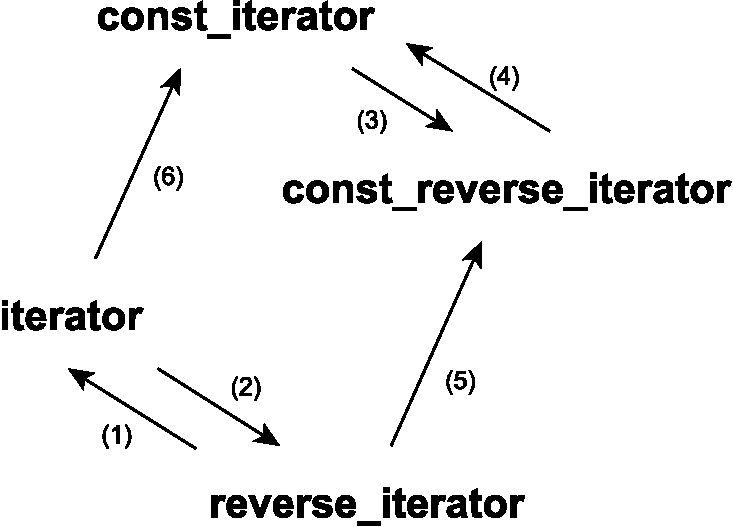
\includegraphics[width=0.7\textwidth]{illustrations/itersdiag-crop.pdf}
\caption{Диаграмма преобразований для итераторов}
\label{fig:itersdiag}
\end{figure}

Здесь стрелки отмечены цифрами:

\begin{itemize}
\item \textbf{(1-4)} Обращение итератора
\begin{lstlisting}
auto rit = make_reverse_iterator(it);
auto it = rit.base();
\end{lstlisting}
\item \textbf{(5, 6)} Добавление константности
\begin{lstlisting}
Cont::const_iterator cit = it;
Cont::const_reverse_iterator crit = rit;
\end{lstlisting}
\end{itemize}

В случаях 5 и 6, нужно иметь контейнер, чтобы выполнить приведение. Из диаграммы видна самая главная проблема: из константного итератора, как с Дону, выдачи нет. Майерс \cite{effectivestl} для аналога \lstinline!const_cast! предлагает использовать advance

\begin{lstlisting}
Iter i(cont.begin());
advance(i, distance<decltype(ci)>(i, ci));
\end{lstlisting}

\textbf{Вопрос к студентам:} зачем явно указан шаблонный параметр для \lstinline!distance!?

\ifanswers
Чтобы избежать неоднозначности вывода типов межу итератором и константным итератором
\fi

Основная проблема с этим подходом: время O(N) для ``неудачных'' контейнеров, таких, как списки. Решение для C++11 известно как ``Hinant trick'' и выглядит забавно.

\begin{lstlisting}
template <typename Container, typename ConstIterator>
typename Container::iterator 
remove_constness(Container& c, ConstIterator it) {
  return c.erase(it, it);
}
\end{lstlisting}

Переход от обратного итерирования к прямому гораздо проще, особенно если понимать как работает функция \lstinline!base!.

\begin{lstlisting}
vector<int> v {1, 2, 3, 4, 5, 6, 7};
auto ri = v.rbegin() + 4; 
auto it = ri.base();
cout << *ri << " " << *it << endl;
\end{lstlisting}

\textbf{Вопрос к студентам:} угадайте, что на экране?

\ifanswers
ответ 3 и 4, пояснения см. далее в тексте
\fi

Чтобы понять, что же на экране, полезно посмотреть на то как выглядит контейнер в прямом и в обратном порядке. Пояснение процесса см. на (рис. \ref{fig:backandforth}).

\begin{figure}[ht]
\centering
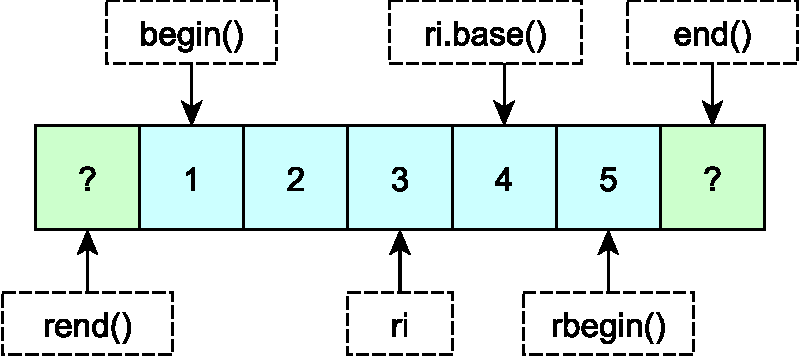
\includegraphics[width=0.7\textwidth]{illustrations/backandforth-crop.pdf}
\caption{Прямое и обратное итерирование}
\label{fig:backandforth}
\end{figure}

Можно думать об итераторе как о стрелочке, которая находится до (прямой итератор) или после (обратный итератор) элемента на который указывает и, при обращении, оборачивается на месте.

\subsection{Адаптеры итераторов}\label{subsub:iteradapt}

Итераторы так же как и контейнеры можно \textbf{адаптировать} и особенно хорошо это видно на примере адаптации по направлению.

Выше уже рассматривался range-based for (см. \ref{PointersToIterators}).

\begin{lstlisting}
for (auto elt : vec)
\end{lstlisting}

Такая запись обходит контейнер vec в прямом порядке.

Можно ли написать адаптер, чтобы обойти тот же контейнер в обратном порядке?

\begin{lstlisting}
for (auto elt : reverse_cont(vec))
\end{lstlisting}

Оказывается да, можно. И, мало того, этот адаптер настолько прост, что его наверняка когда-нибудь стандартизируют.

Сначала следует определить тип, для которого будут переопределены глобальные функции \lstinline!begin! и \lstinline!end!.

\begin{lstlisting}
template <typename T>  struct reversion_wrapper {
  T& iterable;
};
\end{lstlisting}

Теперь собственно переопределение это механическое упражнение, не требующее интеллектуальных усилий.

\begin{lstlisting}
template <typename T> 
auto begin (reversion_wrapper<T> w) {
  return std::rbegin (w.iterable); 
}

template <typename T> 
auto end (reversion_wrapper<T> w) {
  return std::rend (w.iterable); 
}
\end{lstlisting}

И ключевой момент это определение адаптера. Всё что нужно это завернуть входной параметр в должный тип, для которого уже всё переопределено.

\begin{lstlisting}
template <typename T> 
reversion_wrapper<T> reverse_cont (T&& iterable) {
  return { iterable };
}
\end{lstlisting}

Это работает потому, что range-based обход не использует ничего, кроме \lstinline!std::begin! и \lstinline!std::end!.

Ещё одна распространённая стратегия адаптации это inserters -- специальные итераторы, преобразующие запись по итератору во вставку в контейнер.

\subsection{Валидность и инвалидация итераторов}\label{subsub:valinval}

Прежде, чем говорить об инвалидации, следует поговорить о валидности. Валидным может быть тератор или диапазон.

\textbf{Валидный итератор} это такой, который конформно поддерживает все операции для своей категории операторов. Например если валидный форвард-итератор увеличить на единицу, он будет указывать на следующий элемент (или станет невалидным). Если сделать такое с невалидным итератором, результат не будет определён.

\textbf{Валидный диапазон} состоит из двух валидных итераторов, причём второй достижим из первого.

\begin{lstlisting}
istream_iterator<string> beg(ifstream("in.txt")), fin;
cross_copy (beg, fin,
            ostream_iterator<string>(ofstream("out.txt")));
\end{lstlisting}

Диапазон, задаваемый в этом примере парой итераторов (\lstinline!beg!, \lstinline!fin!) невалиден, потому что невалиден итератор \lstinline!beg!. Он является висячим итератором (по аналогии с висячим указателем), так как его файловый поток прекратил своё существование раньше его первого использования.

Итератор может оказаться невалидным по целому ряду причин:

\begin{itemize}
\item Он не инициализирован (т. н. сингулярные итераторы)
\item Он подвис, т.е. ссылается на объект с истекшим сроком жизни
\item Он указывает за пределы диапазона
\item Он инвалидирован операциями над контейнером
\item Это использованный итератор ввода
\end{itemize}

Сингулярные итераторы уже рассматривались ранее и иногда в них нет ничего плохого. Например в примере выше, итератор \lstinline!fin! сингулярен, но вполне валиден. Но вот пример ситуации похуже.

\begin{lstlisting}
list<string>::iterator lstit;
copy (vec.begin(), vec.end(), lstit);
\end{lstlisting}

Здесь сингулярный итератор не валиден и результат копирования не определён (UB). Аналог такого итератора -- неинициализированный указатель.

Итераторы за границами диапазона делятся на два основных типа. Во-первых это итераторы, показывающие на \lstinline!end()! или \lstinline!rend()!, которые можно использовать но нельзя разыменовать (past-the-end итераторы) 

\begin{lstlisting}
list<int> lst;
auto past_end = lst.begin();
cout << *past_end << endl; // fail
lst.insert (past_end, 1); // ok
\end{lstlisting}

Во-вторых это итераторы, показывающие далеко после конца или раньше начала, с которыми нельзя делать ничего (out-of-range).

Итератор также может быть инвалидирован операциями над контейнером

\begin{lstlisting}
vector<int> v = {11, 7, 5, 3, 2};
auto vit = advance (v.begin(), 3);
v.clear();
cout << *vit << endl; // fail
\end{lstlisting}

Здесь итератор может инвалидирован и куда он указывает не определено. К сожалению, если итератор реализован как указатель, он будет куда-то указывать и ошибка может быть ``тихой''.

Но самое плохое, даже не то, что она может быть тихой, а то, что она может быть плавающей. Простой пример.

\begin{lstlisting}
vector<int> v = {2, 3, 5, 7, 11};
auto vit = advance (v.begin(), 3);
v.push_back(13);
cout << *vit << endl; // ok???
\end{lstlisting}

Здесь итератор может быть инвалидирован, если capacity закончилось и случился \lstinline!realloc!. А может и не быть.

Ниже подытожены правила базовой инвалидации для основных контейнеров на вставке и на удалении

\begin{enumerate}
\item Вставка
\begin{itemize}
\item vector -- сохраняются все итераторы до точки вставки кроме случаев перевыделения, кгда все инвалидированы
\item deque -- все итераторы всегда инвалидированы
\item list -- все итераторы сохраняются
\end{itemize}
\item Удаление
\begin{itemize}
\item vector – инвалидируются все итераторы после точки удаления, сохраняются до.
\item deque – инвалидируются все итераторы при удалении из середины. При удалении из начала или конца, все итераторы сохраняются (кроме итертаора на удаляемый).
\item list – сохраняются все итераторы кроме итератора на удаляемый элемент
\end{itemize}
\end{enumerate}

Ну и, пожалуй, самый неочевидный случай инвалидации это использованные input-итераторы

\begin{lstlisting}
ifstream file("in.txt");
istream_iterator<string> beg(infile), end;
cross_copy  (beg, end, ostream_iterator<string>(cout)); // ok
vector<string> vec (beg, end); // fail
\end{lstlisting}

Увы, проход второй раз по файлу невозможен. Хотя казалось бы и файл никуда не делся и вообще всё хорошо. Но нет.

\pagebreak
\section{Алгоритмы}

\hfill\textit{Computer science is no more about computers}

\hfill\textit{than astronomy is about telescopes}{\vspace{0.5em}}

\hfill\textit{-- Edsger W. Dijkstra}

Алгоритмы стандартной библиотеки это тот клей, который связывает контейнеры с итераторами. Контейнеры и итераторы полезны сами по себе, но вместе с алгоритмами они обретают законченность идеи и силу подлинной обобщённости.

Слово ``алгоритм'' сильно перегружено значениями. В контексте стандартной библиотеки, алгоритм это любая функция, которая оперирует на диапазоне, заданном итераторами.

\subsection{Абстракция циклов}

Начать рассмотрение алгоритмов следует с задачи, которая выглядит до обидного просто. Дан контейнер \lstinline!cont!. Необходимо к каждому его элементу применить функцию \lstinline!func!. 

\begin{lstlisting}
template <typename C, typename F> 
void apply (C cont, F func) 
{
  // here goes some code
}
\end{lstlisting}

Программист с опытом на языках вроде C практически на автомате написал бы здесь нечто очевидное.

\begin{lstlisting}
for (auto it = cont.begin(); it != cont.end(); ++it)
  func (*it);
\end{lstlisting}

Человек, который дошёл до этой строчки, читая эту главу с начала, наверняка вспомнил бы также про range-based for (см. \ref{PointersToIterators}) и улучшил ситуацию, сократив код.

\begin{lstlisting}
for (auto elt : cont)
  func (elt);
\end{lstlisting}

Однако человек, действительно осознавший стандартную библиотеку, выбрал бы следующий (несколько странно выглядящий) вариант.

\begin{lstlisting}
for_each (cont.begin(), cont.end(), func);
\end{lstlisting}

Здесь \lstinline!std::for_each! это алгоритм (т.е. см. выше, функция) с сигнатурой

\begin{lstlisting}
template<typename InputIterator, typename Func>
for_each (InputIterator fst, InputIterator lst, Func f);
\end{lstlisting}

С первого взгляда не ясно почему вызов функции вместо простого цикла это хорошая идея (и со второго). Тем не менее, это хорошая идея. Можно привести аргумент из C++17. Там вариант с \lstinline!std::for_each! может быть переписан с учётом возможного параллелизма.

\begin{lstlisting}
for_each (std::execution::par, cont.begin(), cont.end(), func);
\end{lstlisting}

Распараллелить так же просто цикл вряд ли получится. Кроме того, сама функция может быть реализована в стандартной библиотеке куда эффективней, потому что разработчик знает, что она делает. Можно рассматривать её как своего рода ``специализацию'' цикла. Видя в коде цикл общего вида, компилятор может применить лишь ограниченное количество оптимизаций, так как он не понимает и не может понимать что имелось в виду. Но каждый специализированный класс циклов задаваемый стандратной библиотекой служит лишь какой-то одной цели и может выполнять эту цель куда как эффективней.

В результате применение алгоритмов не только абстрагирует конкретные действия и улучшает читаемость кода, но может улучшить и его быстродействие. Такие абстракции (а все мы привыкли к тому, что абстракции не бесплатны) называются \textbf{абстракциями с отрицательной стоимостью}.

\subsection{Копирование и суффиксы для алгоритмов}

В стандартной библиотеке алгоритмов действительно много. Ещё в 98-м году их было около ста и с тех пор их число увеличивалось, сейчас приближаясь к 130 (точный подсчёт связан с некими сложностями в методологии, например считать ли алгоритмом стандартной библиотеки доставшийся от C qsort). К счастью, нет никакой необходимости учить их все. В именовании алгоритмов есть своя система, понимая которую можно выучить не более чем 30-40 корней, получив все остальные даром.

Для примера, можно взять алгоритм \lstinline!copy!. 

\begin{lstlisting}
template<class InputIterator, class OutputIterator> OutputIterator
copy (InputIterator first, InputIterator last, OutputIterator result)
\end{lstlisting}

Его паттерн следующий:

\begin{lstlisting}
// copy pattern
for (auto it = first; it != last; ++it)
  *result++ = *it;
\end{lstlisting}

Но в его имени (как и в имени других алгоритмов) могут быть \textbf{суффиксы}. Кроме того, суффиксом может быть само слово \lstinline!copy!. Основные суффиксы это:

\begin{itemize}
\item \textbf{if} (например \lstinline!copy_if!) -- означает, что алгоритм принимает дополнительный предикат и что действие будет выполнено, только если этот предикат истинный. В случае копирования, в его паттерн добавляется условие.

\begin{lstlisting}
// copy_if pattern
for (auto it = first; it != last; ++it)
  if (pred(*it))
    *result++ = *it;
\end{lstlisting}

\item \textbf{n} (например \lstinline!copy_n!) -- означает, что алгоритм принимает дополнительно количество раз, которые он должен выполнить своё действие.

\begin{lstlisting}
// copy_n pattern
for (size_t i = 0; i != n; ++i)
  *dst++ = *src++;
\end{lstlisting}

\item \textbf{copy} (например \lstinline!reverse_copy! означает, что обращённая последовательность должна быть размещена в новой памяти, а не развёрнута на месте как в случае \lstinline!reverse!). Ну и в целом для любого алгоритма означает, что он копирует свой результат в новое место, не используя старое.
\end{itemize}

Тут полезно разобрать несложный пример.

\begin{lstlisting}
int myints[] = {2, 3, 5, 7, 11, 13, 17}; 
vector<int> myvector (7);

copy_n (myints, 7, myvector.begin());
copy (myvector.begin(), myvector.end(), 
      ostream_iterator<int>(cout, "\n"));

fill (myvector.begin(), myvector.end(), 0);
copy_if (myints, myints+7, myvector.begin(), 
         [](int i){ return (i % 3) == 1; });
copy (myvector.begin(), myvector.end(), 
      ostream_iterator<int>(cout, "\n"));
\end{lstlisting}

\textbf{Вопрос к студентам:} что на экране?

\ifanswers
Сначала будут выведены через перевод строки все числа 2, 3, 5, 7, 11, 13, 17, а потом, тоже через перевод строки, будут выведены числа 7, 13, 0, 0, 0, 0, 0, поскольку только эти два числа из перечисленных дают 1 в остатке от деления на 3.
\fi

Паттерны, которые нарисованы выше, конечно полезны. Но жизнь может отличаться и всегда полезно уметь увидеть в существующем коде паттерн.

Вот, например, код.

\begin{lstlisting}
assert (cont.size() >= N);
auto it = cont.begin();
for (size_t idx = 0, idx != N; ++idx, ++it)
  cout << *it << endl;
\end{lstlisting}

\textbf{Вопрос к студентам:} как переписать его алгоритмом?

\ifanswers
Это очевидный случай \lstinline!copy_n! и алгоритм будет соответствующий (здесь \lstinline!tp_! это тип элемента в контейнере).

\begin{lstlisting}
copy_n (cont.begin(), N, ostream_iterator<tp_>(cout, "\n"));
\end{lstlisting}
\fi

Худшее, что тут может произойти: человек может начать видеть алгоритм \lstinline!for_each! во всех циклах, в том числе и в приведённом выше. Это печальная ошибка. Разновидностей алгоритмов много и каждый спецмализирует цикл своим уникальным образом.

\subsection{Общий обзор}

Все алгоритмы можно (сравнительно произвольно) разбить на несколько основных категорий. Может показаться, что вообще-то хватило бы и первых двух: разбиение на модифицирующие и не модифицирующие алгоритмы выглядит исчерпывающим. Стандарт (C++17 28.1) делит алгоритмы на не изменяющие структуру последовательности (non modifying), изменяющие структуру последовательности (mutating) и похожие на сортировку (sorting and related) не считая категории-призрака алгоритмов, унаследованных от языка C. Это похоже на анекдот про три способа делать дело (правильный, неправильный и армейский), но такое усложнение имеет смысл.

Например мы договариваемся классифицировать всё по основному назначению алгоритма. Немодифицирующий алгоритм в этих терминах это просто информационный запрос к контейнеру, в то время, как модифицирующий нужен именно для того, чтобы изменить структуру контейнера. В этом смысле, несомненно, \lstinline!sort! это модифицирующий алгоритм, а \lstinline!is_sorted! -- нет. Но есть нечто большее, связывающее эти два алгоритма: оба они относятся к сортировке и их, поэтому, можно выделить в специальную группу вместе с другими, относящимися к сортировке и разбиению алгоритмами, как модифицирующими, так и не модифицирующими.

Автор этих лекций в итоге остановился на шести основных категориях.

\subsubsection{Немодифицирующие}

\begin{itemize}
\item \lstinline!all!, \lstinline!any!, \lstinline!none!
\item \lstinline!for_each (n)!
\item \lstinline!find (if), count (if)!
\item \lstinline!search, find_end, find_first_of!
\item \lstinline!mismatch!
\item \lstinline!adjacent_find!
\item \lstinline!min (element), max (element), minmax (element)!
\item \lstinline!clamp!
\item \lstinline!equal, lexicographical_compare!
\end{itemize}

Собранные в этой секции алгоритмы делают запрос самого общего вида. Начиная от \lstinline!all! и заканчивая \lstinline!find_first_of! это всё поиск на несортированных контейнерах. При этом даже если контейнер сортированный, они будут работать с ним как с несортированным.
Несколько особняком стоит \lstinline!for_each! потому что он, строго говоря, ничего не запрашивает. Но принцип его работы такой же, как у поиска. Только он ``находит'' все элементы контейнера.
При объяснении на лекциях, наибольший интерес вызывали \lstinline!adjacent_find! и \lstinline!clamp! 

\subsubsection{Модифицирующие}

\begin{itemize}
\item \lstinline!copy (if) (n) (backward)!, \lstinline!move (backward)!
\item \lstinline!swap!, \lstinline!swap_ranges!, \lstinline!iter_swap!
\item \lstinline!transform!
\item \lstinline!replace (copy) (if)!
\item \lstinline!fill (n)!
\item \lstinline!generate (n)!
\item \lstinline!remove (copy) (if)!
\item \lstinline!unique (copy)!
\item \lstinline!reverse!, \lstinline!rotate (copy)!
\item \lstinline!shuffle!
\item \lstinline!sample!
\end{itemize}

Здесь тоже в целом всё понятно. Обычно некое смущение вызывает алгоритм 

\subsubsection{Сортировка и бинарный поиск}

\begin{itemize}
\item \lstinline!is_partitioned!, \lstinline!is_sorted!
\item \lstinline!partition!, \lstinline!stable_partition!
\item \lstinline!sort!, \lstinline!partial_sort!, \lstinline!stable_sort!
\item \lstinline!nth_element!
\item \lstinline!binary_search! 
\item \lstinline!lower_bound!
\item \lstinline!upper_bound!
\item \lstinline!equal_range!
\item \lstinline!merge!
\item \lstinline!includes!
\item set operations: \lstinline!set_difference!, \lstinline!set_intersection!, etc...
\end{itemize}

\subsubsection{Слияния и кучи}

\begin{itemize}
\item \lstinline!is_heap!
\item \lstinline!make_heap!
\item \lstinline!push_heap!
\item \lstinline!pop_heap!
\end{itemize}

\subsubsection{Численные}

\begin{itemize}
\item \lstinline!is_permutation!
\item \lstinline!next_permutation!
\item \lstinline!prev_permutation!
\item \lstinline!accumulate!, \lstinline!reduce!
\item \lstinline!iota!
\item \lstinline!partial_sum!, \lstinline!exclusive_scan!, \lstinline!inclusive_scan!
\item \lstinline!adjacent_difference!
\item \lstinline!inner_product!
\end{itemize}

В этот обзор не вошла работа с неинициализированной памятью (такие функции как \lstinline!uninitialized_default_construct!) и наследство стандартной библиотеки C. Легко подсчитать, что здесь не больше 50 пунктов, которые и определяют основное ядро алгоритмов, вместе с суффиксами и всякой экзотикой.

\subsection{Идиома erase-remove}\label{subsub:eraseremove}

Удаление элементов из контейнера при работе с итераторами имеет свои контринтуитивные особенности. Формально для удаления служит алгоритм \lstinline!std::remove! и здесь может возникнуть искушение воспользоваться им что называется ``в лоб''.

\begin{lstlisting}
std::vector<int>& vec = myNumbers;
std::remove(vec.begin(), vec.end(), number_in);
\end{lstlisting}

Увы это не работает и не может работать. Ни у какого алгоритма не может быть достаточно информации чтобы по паре входных итераторов произвести честное удаление из обобщенного контейнера, потому что это потребовало бы от них по сути прямого управления памятью контейнера. Что происходит на самом деле проиллюстрировано ниже:

\begin{figure}[h!]
\centering
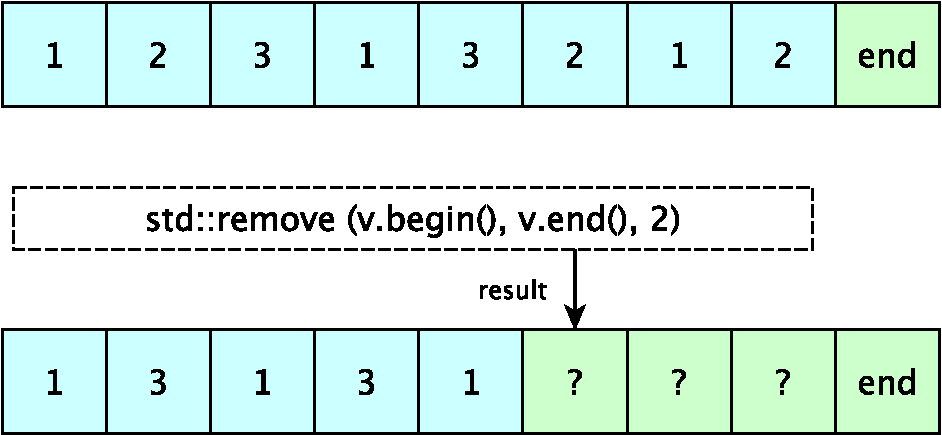
\includegraphics[width=0.9\textwidth]{illustrations/erase-remove-crop.pdf}
\caption{Идиома erase-remove}
\label{fig:erase_remove}
\end{figure}

Произошел сдвиг всех элементов, попадающих под условие удаления в хвост контейнера. Далее чтобы действительно очистить контейнер, нужно вызвать его метод \lstinline!erase! например так:

\begin{lstlisting}
vector<int>& vec = myNumbers;
vec.erase(remove(vec.begin(), vec.end(), number_in), vec.end());
\end{lstlisting}

Этот код записывается слитно очень часто, так что такие паттерны, как использование этой идиомы, опытный разработчик должен распознавать в коде ``на лету''.

Мало того, опознавать идиому erase-remove нужно также в тех случаях, когда там вообще нет remove. Мало ли алгоритмов удаляют данные. Вот, например, unique

\begin{lstlisting}
vector v = {1, 42, 2, 42, 3, 42, 4};
sort (v.begin(), v.end());
v.erase (unique (v.begin(), v.end()), v.end());
\end{lstlisting}

К счастью, в стандартной библиотеке таких алгоритмов мало (собственно \lstinline!remove!, \lstinline!remove_if! и \lstinline!unique!), но в пользовательском коде может встретиться всякое.

\subsection{Абстракция циклов}

TODO: перенести со слайдов и поставить ссылку на Парента \cite{talk:parent:seasoning}

\subsection{Трансформации}

В функциональных языках люди очень любят функции вроде \lstinline!map!, которые абстрагируют применение функтора к последовательности с порождением другой последовательности. В терминах какого-нибудь Haskell, это нечто вроде:

\begin{verbatim}
map :: (a -> b) -> [a] -> [b]
\end{verbatim}

Для C++ роль такой функции выполняет \lstinline!transform!. Он до некоторой степени похож на \lstinline!for_each! до степени смешения. Поэтому важно понимать, что у этих функторов разные соответсвующие им паттерны циклов.

Например обратить знак у последовательности целых чисел легко как с помощью одного, так и с помощью другого, но паттерн применения принципиально разный.

\begin{lstlisting}
  vector<int> v = {2, 3, 5, 7, 11, 13};

  // Option 1.
  for_each(v.begin(), v.end(), [] (auto& i) { i = -i; } );

  // Option 2.
  transform (v.begin(), v.end(), v.begin(), [] (auto i) { return -i; } );
\end{lstlisting}

Из этих двух вариантов, предпочтителен \lstinline!transform!, так как ничего не утекает по косвенности. 

Но главное их отличие в другом: в отличии от \lstinline!for_each!, \lstinline!transform! \textbf{не гарантирует порядка выполнения}. Программист указывает трансформировать последовательность, но не говорит как конкретно это сделать.

TODO: в слайдах у меня тут функторы против лямбд. Должно ли это быть здесь или вынести это -- вопрос.

На примере \lstinline!transform! можно разобрать неожиданные проблемы, возникающие при попытке применять контейнеры с перегруженными функторами. Общеизвестна функция \lstinline!toupper!, приплывшая в C++ из стандартной библиотеки языка C. Попытка применить её как аргумент для трансформации строчки натыкается на небольшую проблему.

\begin{lstlisting}
string s="hello";
transform(s.begin(), s.end(), s.begin(), std::toupper);
\end{lstlisting}

Небольшая проблема (с сообщением об ошибке примерно на два экрана) сводится к тому, что этот вариант не компилируется. Не компилируется он, как и было сказано, поскольку, приплыв из стандартной библиотеки C, \lstinline!toupper! раздвоилась (такое бывает). C++ знает её уже в двух вариантах:

\begin{lstlisting}
charT toupper(charT) const;
const charT* toupper(charT* low, const charT* high) const;
\end{lstlisting}

Вызов \lstinline!transform! не содержит достаточного контекста для разрешения перегрузки. Выходов (простых) тут два. Во-первых можно разрешить перегрузку вручную явным приведением типа. Во-вторых можно создать контекст, обернув всё в лямбда функцию.

\begin{lstlisting}
transform(s.begin(), s.end(), s.begin(),
          static_cast<int(*)(int)>(std::toupper));

transform(s.begin(), s.end(), s.begin(), 
          [](auto x){ return std::toupper(x); });
\end{lstlisting}

Эстетика радуется второму варианту, но формально первый вариант создаёт на одну косвенность меньше, так что кто знает. 

TODO: transform и move семантика. Требует рассмотрения move итераторов, а это адаптер.

\subsection{Бинарный поиск и его варианты}

До сих пор рассматривались алгоритмы, которые не накладывали никаких неявных ограничений на диапазон (кроме валидности, но валидность нужна всегда). Но не все алгоритмы столь няшно доброжелательны. Некоторые алгоритмы, самым известным из которых является бинарный поиск, требуют отсортированного интервала и работают на неотсортированном непредсказуемо.

\begin{lstlisting}
vector<int> v = {81, 9, 54, 36, 27, 63, 18, 72, 45};
sort (v.begin(), v.end());
if (binary_search (v.begin(), v.end(), 37) {
  assert (0 && "Oh, no!");
}
\end{lstlisting}

Как видно из примера выше, алгоритм, который имеет многообещающее название \lstinline!binary_search!, на самом деле ничего не находит. Он возвращает логическое значение -- есть элемент в контейнере или его там нет.

\subsection{Алгоритмический подход к перестановкам}\label{subsub:transpositions}

Методы абстракции, рассмотренные в этой главе, простираются далеко за пределы стандартной библиотеки. Вовсе не обязательно иметь стандартные контейнеры, итераторы и так далее, чтобы использовать эти подходы.

Для примера, здесь будет рассмотрена такая далёкая от стандартной библиотеки вещь, как перестановки.

Мы можем кодировать перестановки любых объектов как циклические перестановки. Простейший цикл это (1 2) означает, что 1 переходит в 2 и 2 переходит в 1, то есть 1 и 2 меняются местами. Цикл (2 3 1) означает $2 \rightarrow 3$ , $3 \rightarrow 1$, $1 \rightarrow 2$.

Очевидно, что (1 2 3) == (2 3 1) == (3 1 2). Изо всех равных циклов можно выбрать один у которого наименьший элемент стоит первым в записи цикла. Это будет (1 2 3) и этот цикл называется нормальной формой записи своего класса эквивалентности.

\textbf{Вопрос к студентам:} какая будет нормальная форма для (4 2 1 3)?

\ifanswers
Правильный ответ: разумеется (1 3 4 2)
\fi

Думать о перестановках в терминах циклов несколько необычно. Обычно о перестановках думают как о двух столбиках, первый из которых задаёт начальную строчку, а второй строчку после перестановки.

\[
  \left(\begin{matrix}
    1 & 2 & 3 & 4 & 5 & 6 & 7 & 8 & 9  \\
    9 & 2 & 3 & 1 & 7 & 6 & 8 & 5 & 4
  \end{matrix}\right)
\]

Вся информация при этом сконцентрирована в нижнем столбике, поскольку верхний тривиален.

Необходимо написать функцию, которая переводит нижний столбик записи перестановки в циклическую форму. В данном случае ответом будет (1 9 4)(2)(3)(5 7 8)(6).

Для начала нужно ответить на вопрос какая у этой функции будет сигнатура.

Пожалуйста прежде чем читать дальше выпишите самостоятельно сигнатуру которую вы предлагаете.

Если вы выписали нечто вроде

\begin{lstlisting}
// creates array of loops from permutation given by table
// say: a, g, [d, c, e, g, b, f, a]
// gives: [(a, d, g), (b, c, e), (f)]
template <typename T>
void create_loops(T start, T fin, const vector<T>& table,
                  vector<PermLoop<T>>& out);
\end{lstlisting}

То поздравляю, вы ничего не поняли про алгоритмы.

Во-первых кодировать диапазон как (start, fin) явными параметрами крайне избыточно. Лучше предположить, что тип \lstinline!T! это домен у которого уже есть и \lstinline!T::start! и \lstinline!T::fin! (или, скажем \lstinline!perm::start(T)! и \lstinline!perm::fin(T)!).

Во-вторых ограничение входного типа вектором и, хуже того, всем вектором сразу, делает эту функцию далёкой от обобщённости. Но казалось бы мы же уже изучали обобщённые алгоритмы. Почему не сделать эту функцию берущей итераторы.

Близкий к совершенству ответ выглядит так:

\begin{lstlisting}
template <typename RandIt, typename OutIt>
void create_loops(RandIt tbeg, RandIt tend, OutIt lbeg);
\end{lstlisting}

Теперь эта функция -- обобщённый алгоритм. Можно реализовать её, но это техническое упражнение, а здесь хочется сконцентрироваться на идеях.

Теперь применение циклов перестановок. Применение это метод в классе \lstinline!PermLoop<T>! и перестановка может применяться как к числу, так и к вектору. Применение (1 2) к числу 1 даёт 2. Применение (1 3) к вектору [1 2 3 4 5 6] даёт в итоге [3 2 1 4 5 6].

Метод \lstinline!apply! для числа это простое применение цикла, использующее в частности другие алгоритмы STL, например \lstinline!find!.

\begin{lstlisting}
template <typename T> T PermLoop<T>::apply (T x) const {
  auto it = find(loop_.begin(), loop_.end(), x);
  if (it == loop_.end()) return x;
  auto nxt = next(it);
  if (nxt == loop_.end()) return *loop_.begin();
  return *nxt;
}
\end{lstlisting}

Сигнатура метода apply для таблицы это снова обобщённый алгоритм, берущий пару итераторов и применяющий перестановку к диапазону.

\begin{lstlisting}
template <typename T>
template <typename RandIt>
void PermLoop<T>::apply(RandIt tbeg, RandIt tend) const;
\end{lstlisting}

Имя типа и тут и в предыдущем примере подсказывает, что требуются итераторы с произвольным доступом.

Теперь настало время заняться действительно интересной вещью: перемножить перестановки. До сих пор перестановки комбинировались когда они были независимы, например (1 2 4)(3 5).

Но что мешает скомбинировать зависимые перестановки?

Запись (1 2)(2 3) означает $1 \rightarrow 2$ , $2 \rightarrow 1$ и далее $2 \rightarrow 3$ , $3 \rightarrow 2$. В итоге получается, что 1 переходит в 2 а потом в 3, значит 1 переходит в 3, 3 в 2, а 2 в 1.

В циклической записи (1 2)(2 3) = (1 3 2)

Более сложный пример: (1 3 2)(1 2 4)(1 4 3 2) = (1 2)(3)(4)

Какую сигнатуру должна иметь функция перемножения (упрощения массива циклов) перестановок?

И опять есть неправильный, но соблазнительный вариант

\begin{lstlisting}
template <typename T>
void simplify_loops (vector<PermLoop<T>> &input);
\end{lstlisting}

\textbf{Вопрос к студентам:} самостоятельно перечислить все его проблемы.

\ifanswers
Ответ: в общем всё довольно очевидно и уже было перечислено выше. Вмерзает в код тип контейнера, не поддерживается часть последовательности, всё вот это вот.
\fi

Правильный вариант в алгоритмическом стиле снова использует итераторы.

\begin{lstlisting}
template <typename RandIt, typename OutIt>
void simplify_loops (RandIt tbeg, RandIt tend, OutIt lbeg);
\end{lstlisting}

Реализация этого алгоритма происходит в терминах двух уже определённых ранее алгоритмов, комбинируя их благодаря механизму итераторов

\begin{lstlisting}
template <typename RandIt, typename OutIt>
void simplify_loops (RandIt tbeg, RandIt tend, OutIt lbeg) {
  using T = typename std::decay<decltype(*tbeg)>::type::value_type;
  vector<T> table(T::fin - T::start + 1, T::start);
  iota(table.begin(), table.end(), T::start);
  for (auto loopit = make_reverse_iterator(tend);
       loopit != make_reverse_iterator(tbeg);
       ++loopit)
    loopit->apply(table.begin(), table.end());
  create_loops(table.begin(), table.end(), lbeg);
}
\end{lstlisting}

Это очень важный код, над ним можно немного помедитировать. Он показывает как в максимально далёкой от стандартной библиотеки предметной области действуют те же подходы, что применялись Степановым и при разработке библиотеки. Именно это -- подлинная мощь библиотеки и мышления в её терминах.

\pagebreak
\section{Ассоциативные контейнеры}\label{AssociativeContainers}

Ранее в приложении к алгоритмам изучались перестановки (см. \ref{subsub:transpositions}). Перестановки образуют группы.

Группа это множество с транзитивной операцией над множеством, такой, что в множестве относительно этой операции есть единичный элемент и у каждого элемента есть обратный. Перемножение перестановок является групповой операцией над множеством перестановок. Единичная перестановка это перестановка, оставляющая всё на местах.

Группа может быть сгенерирована, когда задан только единичный элемент и несколько генераторов, а остальные элементы группы получаются последовательными применениями генераторов к новым элементам.

\begin{figure}[ht]
\centering
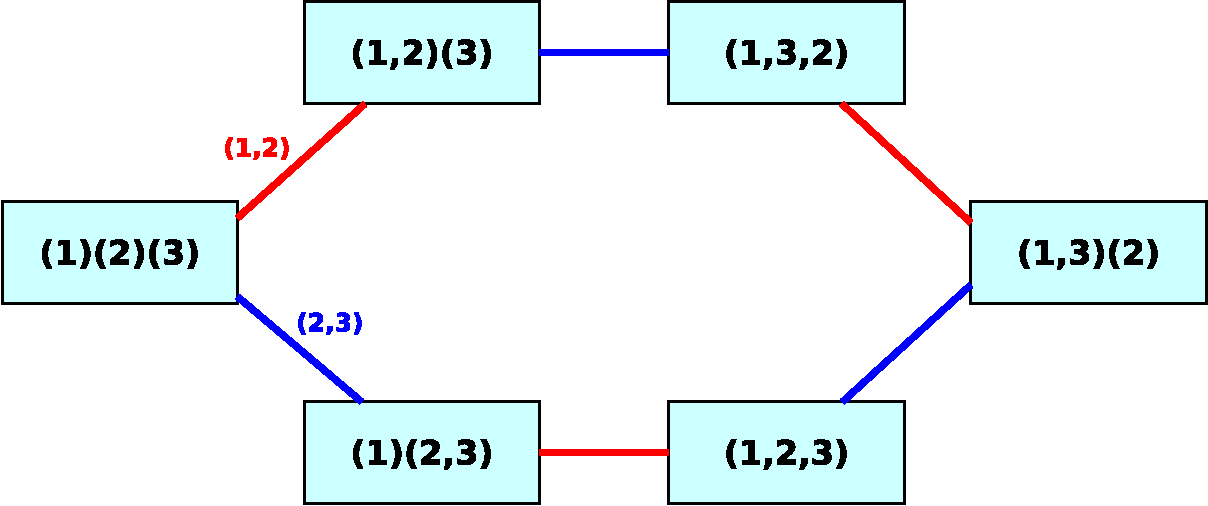
\includegraphics[width=0.9\textwidth]{illustrations/group-base-crop.pdf}
\caption{Группа перестановок S(3)}
\label{fig:group_base}
\end{figure}

На (рис. \ref{fig:group_base}) приведена группа перестановок Sym(3) с генераторами (1, 2) и (2, 3). Первый показан красными линиями, второй -- синими. По линиям можно двигаться в обоих направлениях, так как умножение на цикл длиной два второй раз это просто возврат к предыдущему значению.

Орбитой элемента в группе называются все значения, в которые его переводят элементы группы. Скажем орбита элемента 1 в Sym(3) это (1, 2, 3) как это показано на (рис. \ref{fig:group-orbit}).

\begin{figure}[ht]
\centering
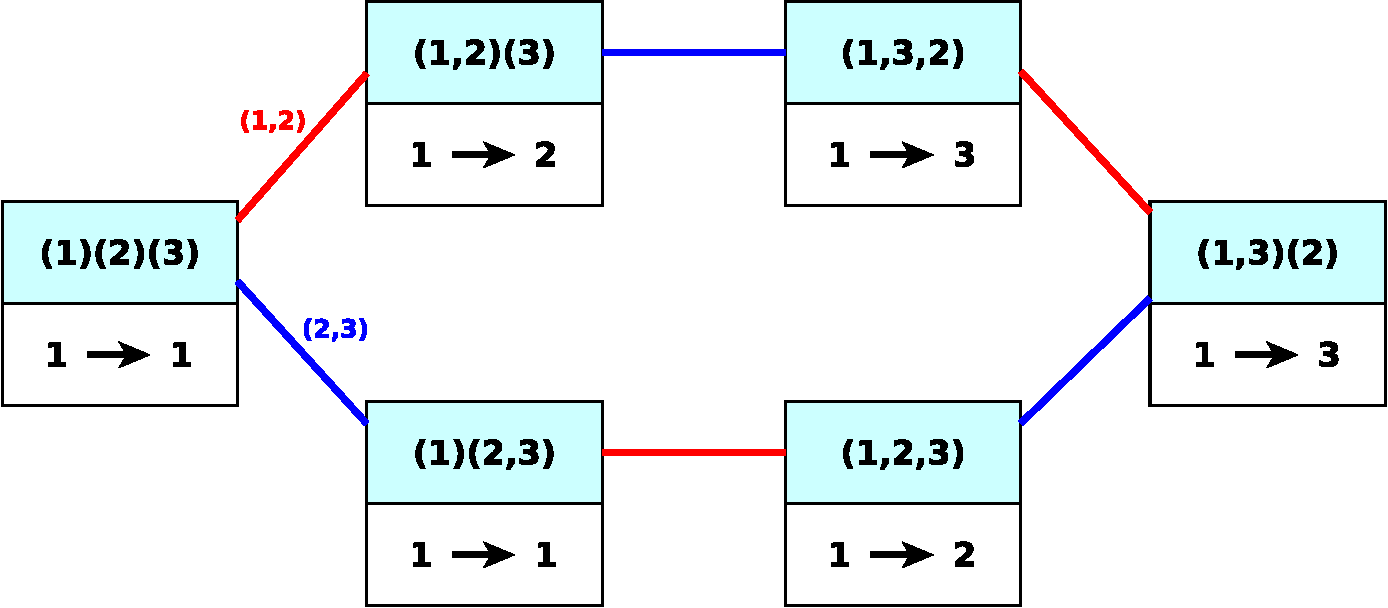
\includegraphics[width=0.9\textwidth]{illustrations/group-orbit-crop.pdf}
\caption{Орбита элемента 1 в S(3)}
\label{fig:group-orbit}
\end{figure}

Вычисление орбиты естественно производить методом транизитивного замыкания. Идёт обход неявного дерева с отсечением ветвей, как показано на (рис. \ref{fig:group-traverse})

\begin{figure}[ht]
\centering
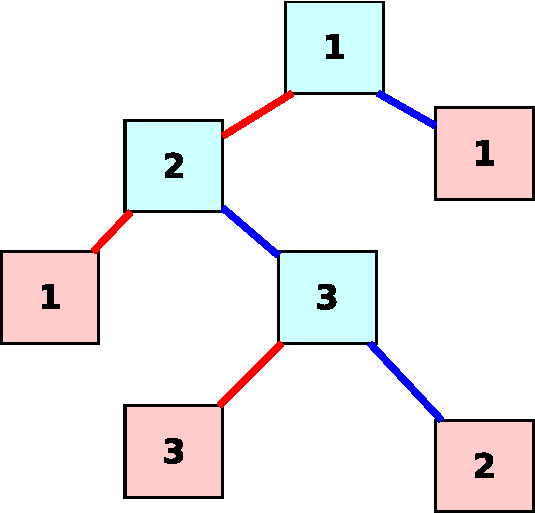
\includegraphics[width=0.4\textwidth]{illustrations/group-traverse-crop.pdf}
\caption{Обход группы и вычисление орбиты}
\label{fig:group-traverse}
\end{figure}

Если написать процедуру, делающую такой обход в обобщённом стиле, то она будет выглядеть как-то так.

\begin{lstlisting}
template<typename T, typename RandIt>
auto simple_orbit(T num, RandIt gensbeg, RandIt gensend) {
  vector<T> orbit, next = {num};
  while (!next.empty()) {
    vector<T> tmp {};
    orbit.insert(orbit.end(), next.begin(), next.end());
    for (const auto &elem : next)
      for (auto igen = gensbeg; igen != gensend; ++igen)
        if (auto newelem = igen->apply(elem); 
            find(orbit.begin(), orbit.end(), newelem) == orbit.end())
          tmp.push_back(newelem);
    next.swap(tmp);
  }
  orbit.erase(unique(orbit.begin(), orbit.end()), orbit.end());
  return orbit;
}
\end{lstlisting}

\textbf{Вопрос к студентам:} оцените алгоритмическую сложность этой процедуры?

\ifanswers
Из-за внутреннего цикла это что-то вроде $O(N^{2}*r)$
\fi

Даже если вы не можете дать ответ на этот вопрос (в конце концов это лекции по C++ а не по алгоритмам), хорошему программисту всё равно очевиден источник основных проблем с производительностью в этой процедуре. Если вам он не очевиден, не расстраивайтесь, вы просто несколько нейроотличны, возьмите профилировщик.

Разумеется, линейный поиск внутри трёх вложенных циклов это вот прямо то чего мы всегда хотели от жизни. Можно ли улучшить? Наверное да. Если вектора сортированные, то поиск мог бы быть бинарным.

\begin{lstlisting}
template<typename T, typename RandIt>
auto simple_orbit(T num, RandIt gensbeg, RandIt gensend) {
  vector<T> orbit, next = {num};
  while (!next.empty()) {
    vector<T> tmp {};
    orbit.insert(orbit.end(), next.begin(), next.end());
    sort(orbit.begin(), orbit.end());
    for (const auto &elem : next)
      for (auto igen = gensbeg; igen != gensend; ++igen)
        if (auto newelem = igen->apply(elem); 
            !binary_search(orbit.begin(), orbit.end(), newelem))
          tmp.push_back(newelem);
    next.swap(tmp);
  }
  orbit.erase(unique(orbit.begin(), orbit.end()), orbit.end());
  return orbit;
}
\end{lstlisting}

Теперь сложность понизилась до $O(N*ln(N)*r)$ но печальная необходимость сортировать вектор каждый раз даёт довольно большую константу при этой асимптотике.

Было бы здорово, если бы был контейнер, который сам поддерживал свою отсортированность и позволял быструю вставку элементов, при этом поддерживая их уникальность. И такой контейнер есть. Это множество \lstinline!std::set!.

\subsection{Множества}

В стандартной библиотеке классы множества и мультимножества
определены следующим образом

\begin{lstlisting}
template <class Key, class Compare = less<Key>,
          class Allocator = allocator<Key>>
class set;

template <class Key, class Compare = less<Key>,
          class Allocator = allocator<Key>>
class multiset;
\end{lstlisting}

На базовом уровне можно думать о множестве как о всегда отсортированном массиве уникальных элементов, не вдаваясь в то, чем оно на самом деле является.

Множество хранит уникальные элементы

\begin{lstlisting}
set<int> s = {67, 42, 141, 23, 42, 106, 15, 50};
for (auto elt : s)
  cout << elt << endl;
\end{lstlisting}

Здесь дважды упомянуто число 42. Ничего не сломается, но на экране будет

\begin{verbatim}
15, 23, 42, 50, 67, 106, 141
\end{verbatim}

С помощью множеств, функция \lstinline!simple_orbit! может быть переписана гораздо проще.

\begin{lstlisting}
template<typename T, typename RandIt>
auto simple_orbit(T num, RandIt gensbeg, RandIt gensend) {
  set<T> orbit, next = {num};
  while (!next.empty()) {
    set<T> tmp {};
    orbit.insert(next.begin(), next.end());
    for (const auto &elem : next)
      for (auto igen = gensbeg; igen != gensend; ++igen)
        if (auto newelem = igen->apply(elem); orbit.count(newelem) == 0)
          tmp.insert(newelem);        
    next.swap(tmp);
  }
  return orbit;
}
\end{lstlisting}

Простой замер производительности показывает, что речь идёт о выигрыше в разы по сравнению с сортированными векторами.

Множества создают упорядочение своих элементов.

\begin{lstlisting}
set<int> s = {67, 42, 141, 23, 42, 106, 15, 50};
auto itb = s.lower_bound(30);
auto ite = s.upper_bound(100);
\end{lstlisting}

Теперь можно итерировать в интервале [30, 100) независимо от того есть ли в точности во множестве такие элементы.

\begin{lstlisting}
for (auto it = itb; it != ite; ++it)
  cout << *it << endl;
\end{lstlisting}

\textbf{Вопрос к студентам:} что будет выведено на экран?

\ifanswers
Правильный ответ: 42, 50, 67
\fi

Второй шаблонный параметр подсказывает, что множества позволяют задавать порядок итерирования

\begin{lstlisting}
set<int, greater<int>> s = {67, 42, 141, 23, 42, 106, 50};
auto itb = s.lower_bound(30);
auto ite = s.upper_bound(100);
\end{lstlisting}

Увы, теперь интервал некорректен. С точки зрения предиката \lstinline!greater! число 100 предшествует числу 30 и таким образом итератор \lstinline!ite! не достижим из \lstinline!itb! (см. \ref{subsub:valinval}).

Запись, вроде приведённой ниже

\begin{lstlisting}
auto itb = s.lower_bound(100);
auto ite = s.upper_bound(30);
\end{lstlisting}

Создаёт валидный диапазон для множества с предикатом \lstinline!greater!. Увы, это никак не контролируется на этапе компиляции.

Интересный вопрос: что будет если упорядочить по критерию ``меньше или равно'' например таким образом

\begin{lstlisting}
set<int, less_equal<int>> s = {67, 42, 141, 23, 42, 106, 50};
\end{lstlisting}

В получившемся множестве тогда окажется два элемента со значением 42. Это нарушает инвариант контейнера и может привести к странным сложно отлавливаемым багам.

Это наводит на мысль, что не каждый предикат подходит для упорядоченного контейнера. И действительно, общая концепция, которой можно проверить годность предиката называется strict weak ordering. Она включает

\begin{enumerate}
\item Антисимметричность $pred(x,y) \Rightarrow \neg pred(y,x)$
\item Транзитивность $pred(x,y) \wedge pred(y,z) \Rightarrow pred(x,z)$
\item Иррефлексивность $\neg pred(x,x)$
\item Транзитивность эквивалентности 
$eq(x,y) \equiv \neg pred(x,y) \wedge \neg pred(y,x)$ 
$eq(x,y) \wedge eq(y,z) \Rightarrow eq(x,z)$
\end{enumerate}

Она же распространяется на предикаты в алгоритмах сортировки и т.д.

\textbf{Домашняя наработка:} пусть $(a + ib < c + id) \Leftrightarrow (a < c) \wedge (b > d)$ является ли это strict weak ordering для комплексных чисел?

Концепция strict weak ordering важна даже в мультимножествах, где казалось бы нет проблемы хранить два одинаковых элемента. Майерс \cite{effectivestl} приводит красивый контрпример

\begin{lstlisting}
multiset<int, less_equal<int>> s;
s.insert(10); // insert 10A
s.insert(10); // insert 10B
\end{lstlisting}

Теперь \lstinline!equal_range! для 10 вернёт пустой интервал, поскольку искомое значение 10 не будет опознано как равное двум уже вставленным.

\subsection{Модификация множеств}

Простейшая модификация элемента множества на месте не работает и работать не должна

\begin{lstlisting}
*s.begin() = 3; // error: assignment of read-only location
\end{lstlisting}

В самом лучшем случае это ошибка компиляции. В худшем случае ваша реализация не поддерживает хранения контантных ключей в множестве и у вас проблемы.

Дело в том, что внутренне множество скорее всего будет пресдтавлено какой-либо разновидностью сбалансированного дерева. Изменение ключа нарушает балансировку и не должно производиться иначе, чем методами класса.

По этой же причине для множеств не работает идиома erase-remove

\begin{lstlisting}
set<int> s = {1, 2};
s.erase(remove(s.begin(), s.end(), 1), s.end());
\end{lstlisting}

В лучшем случае это тоже ошибка компиляции. Удалять из множеств, сохраняя балансировку законно только через их внутренний метод erase.

\begin{lstlisting}
s.erase(1);
\end{lstlisting}

Правда тут тоже есть проблема. Используя такое удаление в цикле слишком легко выстрелить себе в ногу.

\begin{lstlisting}
for (auto it = s.begin(); it != s.end(); ++it)
  if ((*it < 100) && (*it > 30))
    s.erase(it);
\end{lstlisting}

Это очень плохой код, никогда так не делайте. Дело в том, что удаляя элемент вы инвалидируете итератор на этот элемент. Ну и всё. Далее итерация по невалидному итератору заитерирует вас туда, куда Макар телят итерировал.

Решение этой проблемы в C++98 выглядело как-то вот так

\begin{lstlisting}
for (auto it = s.begin(); it != s.end();)
  if ((*it < 100) && (*it > 30))
    s.erase(it++);
  else
    ++it;
\end{lstlisting}

Начиная с C++11, метод erase в множествах возвращает итератор на валидный элемент и этим можно наслаждаться.

\begin{lstlisting}
for (auto it = s.begin(); it != s.end();)
  if ((*it < 100) && (*it > 30))
    it = s.erase(it);
  else
    ++it;
\end{lstlisting}

Не знаю, впрочем, стало ли от этого всем сильно легче.

Если вам (с чего был начат этот параграф) всё-таки нужно заменить элемент в множестве, то методами множества законно делать это только стирая старый элемент и добавляя новый.

\begin{lstlisting}
auto it = s.find(1);
if (it != s.end()) {
  s.erase(it);
  s.insert(3);
}
\end{lstlisting}

Именно эта чувствительность множеств -- тот факт, что они хранят только ключи и всё, делает их в некоторых контекстах очень плохим выбором для контейнера.

\subsection{Отображения}

Если внимательно рассмотреть орбиту элемента 1 в Sym(3) (рис. \ref{fig:group-orbit}), можно заметить, что из шести перестановок группы ровно две оставляют 1 на месте, две превращают его в 2 и две превращают его в 3. Эта симметрия не случайна и за ней лежит некая математическая теория, выходящая за пределы этого конспекта. Но кажется очевидным, что для любого элемента орбиты должен быть элемент группы (называемый также coset representative) который сдвигает элемент, для которого ищется орбита в элемент орбиты.

Пусть стоит задача найти все такие элементы.

Имея только множества, лучшее, что можно придумать это множество пар (элемент, перестановка).

\begin{lstlisting}
template<typename T, typename RandIt>
auto orbit_reps(T num, RandIt gensbeg, RandIt gensend) {
  set<pair<T, Permutation<T>>> orbit;
  Permutation<T> id {};
  set<pair<T, Permutation<T>>> next {{num, id}};
  while (!next.empty()) {
    set<pair<T, Permutation<T>>> tmp {};
    orbit.insert(next.begin(), next.end());
    for (auto&& [elem, curgen] : next)
      for (auto igen = gensbeg; igen != gensend; ++igen)
        if (auto newelem = igen->apply(elem);
            find_if(orbit.begin(), orbit.end(), 
             [newelem](auto&& elt) { return (newelem == elt.first); }) == orbit.end())
          tmp.emplace(newelem, product(curgen, *igen));
    next.swap(tmp);
  }
  return orbit;
}
\end{lstlisting}

Но у этого подхода снова есть проблема, при чём та же самая: линейный поиск. Причём тут сложно что то придумать: в контейнере \lstinline!set! есть метод \lstinline!find!, но нет и не может быть \lstinline!find_if!.

\textbf{Вопрос к студентам:} вы понимаете что не так с \lstinline!find_if! для \lstinline!set!.

\ifanswers
Правильный ответ: ключи. Множество хранит ключи, а \lstinline!find_if! предполагает что ключ более сложен, в частности чем-то ограничен и простой поиск по дереву уже не сработает.
\fi

Для решения таких вопросов: хранения ключа и чего-то вроде значения по этому ключу в стандартной библиотеке существуют отображения и мультиотображения. Они объявлены следующим образом

\begin{lstlisting}
template <class Key, class T, class Compare = less<Key>,
class Allocator = allocator<pair<const Key, T>>>
class map;

template <class Key, class T, class Compare = less<Key>,
class Allocator = allocator<pair<const Key, T>>>
class multimap;
\end{lstlisting}

Здесь можно особо отметить класс для которого аллокатор. В отличии от set, здесь нам явно говорят что именно менять нельзя.

С использованием отображений, решение становится простым и ясным

\begin{lstlisting}
template<typename T, typename RandIt>
auto orbit_maps(T num, RandIt gensbeg, RandIt gensend) {
  map<T, Permutation<T>> orbit, next {{ num, {} }};
  while (!next.empty()) {
    map<T, Permutation<T>> tmp {};
    orbit.insert(next.begin(), next.end());
    for (auto&& [elem, curgen] : next)
      for (auto igen = gensbeg; igen != gensend; ++igen)
        if (auto newelem = igen->apply(elem); orbit.find(newelem) == orbit.end())
          tmp.insert({newelem, product(curgen, *igen)});
    next.swap(tmp);
  }
  return orbit;
}
\end{lstlisting}

У отображения, метод find ищет по ключам с логарифмической сложностью. Если мы оцениваем перемножение перестановок дешевле, чем проверку, что перестановка существует, можно убрать \lstinline!if! так как если в отображении ключ уже существует, вставлено ничего не будет. Но мои замеры производительности показывают, что для огромных перестановок это плохая идея, поскольку ключ это что-то вроде целого числа, а значение тут что-то вроде вектора векторов.

\subsection{Модификация отображений}

В приведённом выше листинге есть места, вызывающие подозрение. В первую очередь это вставка.

\begin{lstlisting}
tmp.insert({newelem, product(curgen, *igen)});
\end{lstlisting}

Здесь она сделана через \lstinline!insert!, но ведь есть же \lstinline!emplace!, его не может не быть.

\begin{lstlisting}
tmp.emplace(newelem, product(curgen, *igen));
\end{lstlisting}

Это действительно работает, и, казалось бы, этот метод экономит одно крайне тяжёлое копирование одной крайне тяжёлой пары. Увы, это не так. Майерс в \cite{effmoderncpp} посвятил этому целый совет 42, поэтому не стоит подробно останавливаться здесь. Вкратце: для ассоциативных контейнеров из-за того, что у них при вставке есть также поиск места для вставки в, условно говоря, дерево, узел всё равно должен быть создан довольно рано. Метод \lstinline!emplace! просто заносит его создание внутрь и имеет по сравнению с \lstinline!insert! не лучшую производительность и проблемы с исключениями. Об этом методе (в чистом виде) для ассоциативных контейнеров можно просто забыть.

Третий вариант специфичен только для отображений и предполагает использование квадратных скобок.

\begin{lstlisting}
tmp[newelem] = product(curgen, *igen);
\end{lstlisting}

Использование квадратных скобок для выражения семантики ``обновление-или-вставка'' -- очень странное проектное решение. Его нет ни в множествах ни даже в мультиотображениях. В самих отображениях такое использование квадратных скобок плохо видно в коде и иногда приводит к странным моментам.

\begin{lstlisting}
cout << m[x] << endl;
\end{lstlisting}

Здесь если \lstinline!m! это \lstinline!map!, то вообще-то ключ \lstinline!x! может быть вставлен в отображение!

Впрочем если обновление действительно нужно, использование квадратных скобок эффективно и обоснованно, так что его следует обдумать. В рассматриваемом случае речь не идёт об обновлении, поэтому именно для групп мы его отметаем, но вообще квадратные скобки несмотря на их минусы могут быть удобны.

И, наконец, лучше всего себя показывает четвертый вариант: \lstinline!emplace! с указанием места вставки, так называемый \lstinline!emplace_hint!.

Чтобы его мотивировать, можно рассмотреть не одну строчку а две.

\begin{lstlisting}
if (auto newelem = igen->apply(elem); orbit.find(newelem) == orbit.end())
  tmp.insert({newelem, product(curgen, *igen)});
\end{lstlisting}

И заметить, что здесь дважды делается одна работа: элемент ищется методом \lstinline!find!, а потом ещё раз ищется при вставке через \lstinline!insert! во время поиска позиции для вставки.

\begin{lstlisting}
auto newelem = igen->apply(elem);
auto it = orbit.lower_bound(newelem);
if (it == orbit.end() || it->first != newelem)
  tmp.emplace_hint(it, newelem, product(curgen, *igen));
\end{lstlisting}

Использование \lstinline!emplace_hint! как показано выше позволяет не делать лишней работы, а искать один раз и искать целенаправленно позицию для возможной вставки с использованием \lstinline!lower_bound!.

Стандарт C++17 принёс в модификацию отображений два новшества. Во-первых вытащить из дерева целую ноду, при этом удалив её полностью и ребалансировав дерево можно с помощью \lstinline!extract!.

\begin{lstlisting}
map<int,string> m1 = {{1, "sator"}, {2, "tenet"}, {3, "nope"}};
auto extval = m1.extract(3);
\end{lstlisting}

О том, какого типа получается \lstinline!extval! лучше даже не задумываться: в стандарте он помечен как полностью Implementation defined, вплоть до размера и состава полей. Всё, что от него требуется это определённый набор методов, среди которых самые полезные это \lstinline!key()! и \lstinline!value()!

\begin{lstlisting}
cout << extval.key() << endl; // prints 3
\end{lstlisting}

Во-вторых соединить два отображения в одно теперь можно с помощью \lstinline!merge!

\begin{lstlisting}
map<int,string> m1 = {{1, "sator"}, {2, "tenet"}};
map<int,string> m2 = {{2, "nothing"}, {3, "arepo"},
                      {4, "opera"}, {5, "rotas"}};
m1.merge(m2);
\end{lstlisting}

При этом все элементы \lstinline!m2! по одному вынимаются (например через \lstinline!extract!) и вставляются в \lstinline!m1!. Метод несколько эффективней, чем делать то же самое простым циклом или даже алгоритмом.

\subsection{Словари}

Простая орбита с использованием множеств всё-таки не слишком хороша.

\begin{lstlisting}
for (const auto &elem : next)
  for (auto igen = gensbeg; igen != gensend; ++igen)
    if (auto newelem = igen->apply(elem); 
        orbit.count(newelem) == 0)
      tmp.insert(newelem);
\end{lstlisting}

В главном цикле притаился метод \lstinline!orbit.count!, имеющий, между прочим, сложность O(ln(N)). Этот логарифмический множитель выглядит болезненно и от него хотелось бы избавиться. Обычно для этого надо чем-то пожертвовать.

Основная идея, которую приносят \textbf{словари} это пожертвовать в данном случае упорядоченностью.

Словари определены в стандарте как четыре класса: неупорядоченные множество, мультимножество, отображение и мультиотображение.

Неупорядоченное множество.

\begin{lstlisting}
template<
  class Key, class Hash = hash<Key>, 
  class KeyEqual = equal_to<Key>,
  class Allocator = allocator<Key>
> class unordered_set;
\end{lstlisting}

Почти аналогично: неупорядоченное отображение.

\begin{lstlisting}
template<
  class Key, class T, class Hash = hash<Key>,
  class KeyEqual = equal_to<Key>,
  class Allocator = allocator<pair<const Key, T>>
> class unordered_map;
\end{lstlisting}

Мультимножество и мультиотображение по сути аналогичны.

С использованием неупорядоченного множества, вычисление простой орбиты теперь можно переписать более вдохновляющим образом.

\begin{lstlisting}
template<typename T, typename RandIt>
auto simple_orbit(T num, RandIt gensbeg, RandIt gensend) {
  unordered_set<typename T::type> orbit;
  vector<T> next = {num};
  while (!next.empty()) {
    unordered_set<typename T::type> tmp {};
    orbit.insert(next.begin(), next.end());
    for (const auto &elem : next)
      for (auto igen = gensbeg; igen != gensend; ++igen)
        if (auto newelem = igen->apply(elem); 
            orbit.count(newelem) == 0) // O(1)+
          tmp.insert(newelem);
    next.swap(tmp);
  }
  return orbit;
}
\end{lstlisting}

Теперь сложность, вероятно, улучшилась, поскольку дерево было заменено на хэш. Но у \lstinline!unordered_set! нет методов \lstinline!lower_bound! и \lstinline!upper_bound!

Пляски с \lstinline!typename T::type! связаны с тем, что \lstinline!T! это что-то вроде \lstinline!IDom<unsigned, 1, 7>! и у него просто лень протягивать хэш и равенство, а проще воспользоваться нижележащим примитивным типом. Но вообще, можно, конечно и добавить, чуть позже об этом пойдёт особый разговор (см. \ref{subsub:selfhash}).

Общий гайдлайн такой: если всё, что нужно это ассоциативный массив и его упорядоченность никак не используется, то механическая замена \lstinline!set! на \lstinline!unordered_set! это первое, что следует попробовать.

Самый частый источник проблем при подобного рода замене это требования к интерфейсу типа. Вместо \lstinline!std::less! теперь по умолчанию идут \lstinline!std::hash! и \lstinline!std::equal_to!. В общем случае сделать оператор ``меньше'' проще, чем сравнение и хэш.

\subsection{Переход к неупорядоченности}\label{subsub:selfhash}

Обычный случай это наличие нетривиального класса с методом \lstinline!less!, используемом в операторе ``меньше'', который, скорее всего объявлен вне класса.

\begin{lstlisting}
struct S {
  string first_name, last_name;
  bool less(const S& rhs) const; // для (<)
};
\end{lstlisting}

Задача сделать для этого класса сравнение на равенство. Худшее что можно сделать это определить равенство механически.

\begin{lstlisting}
bool operator==(const S& lhs, const S& rhs) {
  return !lhs.less(rhs) && !rhs.less(lhs);
}
\end{lstlisting}

Гораздо лучше дописать в класс метод equals и определить в его терминах, ну илив  случае с открытым содержимым просто сделать оператор.

\begin{lstlisting}
bool operator==(const S& lhs, const S& rhs) {
  return (lhs.first_name == rhs.first_name) &&
         (lhs.last_name == rhs.last_name);
}
\end{lstlisting}

А вот с собственным хэшем это уже не слишком хорошо работает. Конечно можно напрячь фантазию.

\begin{lstlisting}
result_type 
operator()(argument_type const& s) const noexcept {
  result_type const h1 = hash<string>{}(s.first_name);
  result_type const h2 = hash<string>{}(s.last_name);
  return h1 ^ (h2 << 1);
}
\end{lstlisting}

Сдвиг на единицу нужен для частого случая когда строки одинаковые. В данном случае это работает, но вообще, конечно, хотелось бы механического способа объединения хэшей. В стандарте его нет. На помощь может придти boost, в частности \lstinline!boost::hash_combine!.

\begin{lstlisting}
result_type 
operator()(argument_type const& s) const noexcept {
  result_type const h1 = hash<string>{}(s.first_name);
  result_type const h2 = hash<string>{}(s.last_name);
  size_t seed = 0;
  boost::hash_combine(seed, h1);
  boost::hash_combine(seed, h2);
  return seed;
}
\end{lstlisting}

Но тут, конечно, многие могут не захотеть затаскивать boost в проект и их можно понять. Что же, рано или поздно это стандартизуют.

Кроме всего прочего, наличие в контейнере требования к такой функции, как \lstinline!hash! открывает на уровне стандарта гораздо больше о внутренней структуре контейнера, чем оператор меньше. Относительно упорядоченных множеств и отображений здесь всегда употреблялось слово ``дерево'', но с некоторой осторожностью. Хотя бы просто потому, что ничего в интерфейсе упорядоченных ассоциативных контейнеров не указывает на то, что там \textbf{должно быть} именно дерево. Может и дерево (и то не вполне ясно какое дерево). А может и не дерево вовсе.

А вот неупорядоченные ассоциативные контейнеры это совершенно точно разновидности хеш-таблиц. Тут всё очевидно и двух мнений быть не может. Даже неясно почему слово \lstinline!hash! не внесли в название, как это сделали, например в Ruby.

Но хеш-таблица сама по себе это непрерывный массив корзин (buckets) из которых растут списки коллизий. А это означает, что она имеет много общего с последовательными контейнерами. В частности, что снова можно подумать о резервировании памяти.

\begin{lstlisting}
unordered_map<int, Foo> mapNoReserve;
unordered_map<int, Foo> mapReserve;
mapReserve.reserve(1000);
for(int i = 0; i < 1000; ++i) {
  mapNoReserve.insert({i, Foo()});
  mapReserve.insert({i, Foo()});
}
// ....... control point
\end{lstlisting}

\textbf{Домашняя наработка:} найдите способ замерить полный размер неупорядоченного отображения в памяти. Проведите эксперимент, как в листинге выше. Какой размер в памяти имеют \lstinline!mapReserve! и \lstinline!mapNoReserve! в контрольной точке?

%\subsection{Экзотические контейнеры}
%TODO: flat\_map и bimap?

\pagebreak
\section{Память своими руками}\label{allocators}

\hfill\textit{Allocator relates to allocation, as vector to vexation}{\vspace{0.5em}}

\hfill\textit{-- Andrei Alexandrescu}

В тех языках, где память это ресурс (которых в современном мире уже, пожалуй, меньшинство), выделение и освобождение памяти это точки дополнительной интеллектуальной нагрузки на разработчика. Даже если оставить в стороне ``проклятие меморилика'', выделение и освобождение памяти это всё равно потенциально дорого, а её неупорядоченное использование чревато странным поведением загадочных внутренних структур процессора, таких как кэши.

Стратегия выделения памяти по умолчанию, своего рода один размер, который подходит всем, это выделение с помощью менеджера памяти стандартной библиотеки (для C++ это глобальные операторы \lstinline!new! и \lstinline!delete!). Особенности этого механизма хорошо изучены, задокументированы в стандарте и нацелены на улучшение работы в среднем случае, когда памяти не выделяется ни мало ни много, а объекты аллокации равномерно большие и маленькие. Но что делать людям, чей софт не попадает под средний случай?

Стандартная библиотека C++ сразу была спроектирована таким образом, чтобы каждому контейнеру можно было предоставить собственный аллокатор, решающий вопросы выделения памяти. Например полный шаблон класса \lstinline!vector! выглядит как:

\begin{lstlisting}
template <class T, class A = std::allocator<T> > class vector;
\end{lstlisting}

Если вдуматься, это решение \textbf{странное}. STL проектировалась в 1992 году и не вполне ясно кому и зачем тогда могли понадобиться такие механизмы расширения.

Всё дело в позабытой ныне концепции near и far pointers. Дело в том, что в те годы было модно организовать память сегментами и указатель, показывающий за сегмент, мог иметь вдвое больший размер, чем глядящий внутрь сегмента. Производители аппаратуры предоставляли свои расширения, такие как \lstinline!int * __huge px!, при этом стандарт языка об этом ничего не знал, понимая только обычные указатели, поэтому эти детали нужно было где-то спрятать.

Это повлияло на проектирование аллокаторов. По сути аллокаторы, исходно спроектированные Степановым, должны были знать всего две вещи:

\begin{itemize}
\item Откуда взять память
\item Как преобразовать её к \lstinline!T*! из платформенно-специфичного типа
\end{itemize} 

Таким образом, исходно аллокаторы вообще не планировались как средство выделения памяти. Они планировались как тонкий слой адаптации к настоящему распределителю.

Вынесенные в эпиграф слова Александреску можно с сохранением образности перевести на русский: ``Аллокатор относится к аллокации как барс к барсетке''.

Именно этот факт и создал впоследствии аллокаторам дурную славу: когда люди в итоге начали использовать аллокаторы для того, чтобы определять с их помощью стратегии выделения памяти, они столкнулись с неизбежными проблемами. И именно поэтому в C++ аллокаторы это наиболее часто пересматриваемый механизм: они существенно менялись в почти каждом стандарте, пока, наконец, в C++17 не стали почти совершенными.

Но об этом чуть позже.

\subsection{Простые аллокаторы}\label{sub:stateless}

Итак, вернёмся в 1998 год. Представьте, что у вас есть нестандартный системный распределитель emalloc, который распределяет память в расширенном адресном пространстве (EMS, если кто помнит). И его хочется завести под вектора, списки, и прочие полезные контейнеры.

Простой аллокатор, который всего лишь знает как сбегать к распределителю и принести память, должен выставить использующему его контейнеру две соновные функции аллокаторного интерфейса: \lstinline!allocate! и \lstinline!deallocate!

\begin{lstlisting}
template<typename T> struct ealloc {
  typedef T value_type;
  typedef T* pointer;
  pointer allocate (size_t n) { 
    return static_cast<pointer>(emalloc(n * sizeof(T)));
  }
  void deallocate(pointer p, size_t n) { efree(p); }
};
\end{lstlisting}

Выше показан простой код, с которого вы, вероятно, начали бы. Кажется, что теперь получившийся адаптер можно скормить, например, вектору

\begin{lstlisting}
template <typename T> using s_vector = vector<T, ealloc<T>>;
\end{lstlisting}

Не так быстро. Есть две проблемы и обе стали понятны сообществу как раз где-то к 98-му году.

\begin{enumerate}
\item \textbf{Взаимозаменяемость аллокаторов}

Можно проиллюстрировать так:
\begin{lstlisting}
vector<int, ealloc<int>> v1, v2;
// a lot of code
v1 = v2; // what is happenning here?
\end{lstlisting}
Если аллокатора в каокм-то смысле похож на приведённый выше, то никаких проблем, приваивание и есть присваивание. Но если аллокатор это объект с состоянием, как должно изменяться состояние аллокатора при копировании контейнера?
\item \textbf{Приведение аллокаторов}

Возмём для примера \lstinline!list<T, ealloc<T> >!. Внутри себя список будет создавать не \lstinline!T!, а \lstinline!__list_node<T>!. То есть ему нужно иметь возможность как-то получить для внутреннего использования тип \lstinline!ealloc<__list_node<T> >!, не имеющий с переданным ему \lstinline!ealloc<T>! ничего общего.
\end{enumerate}

Первому вопросу было суждено стать ключевым. Второй изначально казался попроще.

Стандарт 98 года решал первый вопрос просто: все конкретные экземпляры любого типа аллокаторов должны были быть эквивалентны. То есть единственная разумная запись операторов сравнения (и вы как программист должны её предоставить) для приведённого выше \lstinline!ealloc! это следующий код.

\begin{lstlisting}
template <typename T, typename U>
bool operator== (const ealloc<T>&, const ealloc<U>&) {
  return true;
}

template <typename T, typename U>
bool operator!= (const ealloc<T>&, const ealloc<U>&) {
  return false;
}
\end{lstlisting}

Для решения второй проблемы, внутри каждого аллокатора был предусмотрен (опять-таки предоставляемый программистом) шаблонный переходник \lstinline!rebind!

\begin{lstlisting}
template<typename T> struct ealloc {
  // .... all the same ....
  template<typename U> ealloc(const ealloc<U>&) {}
  template<typename U>
  struct rebind { typedef ealloc<U> other; };
};
\end{lstlisting}

Чтобы ещё немножко усложнить жизнь программистам, от вас также требовалось несколько чисто ритуальных движений: предоставить функции \lstinline!construct! и \lstinline!destroy!, выполняющие функции размещающего \lstinline!new! и явного вызова деструктора (причём в реальности у вас не было вариантов написать их существенно иначе, чем показано ниже). Кроме того, от вас требовалась функция \lstinline!max_size! для ограничения общего размера (которую тоже не было возможности сделать особо умной). А также куча синонимов вложенных типов для \lstinline!reference!, \lstinline!const_pointer! и всего такого.

\begin{lstlisting}
template<typename T> struct ealloc {
  // .... all the same ....
  typedef const T* const_pointer;
  typedef T& reference;
  typedef const T& const_reference;
  typedef size_t size_type;
  typedef ptrdiff_t difference_type;

  void construct(pointer p, const T& t) { new(p) T(t); }
  void destroy(pointer p) { p->~T(); }
  size_type max_size() const {
    return numeric_limits<size_type>::max() / sizeof(T);
  }
};
\end{lstlisting}

Все эти вещи были вынесены в traits в C++11 и объявлены устаревшими в C++14.

Вот теперь, пожалуй, всё. Такой аллокатор уже может использоваться в коде на C++98.

И тут, разумеется, встаёт главный вопрос: \textbf{для чего} он может использоваться. Хорошо, допустим предназначение \lstinline!ealloc! было описано выше. Но что если хочется чего-то сложнее, чем просто нужную память подтасиквать и ненужную оттаскивать?

Первое, что приходит на ум это логгирующий аллокатор. Возможна также некая реализация защиты стека. Но что если хочется иметь заранее выделенный пул, где выделялись бы более мелкие объекты? Или, например сделать коалескинг при работе с этим пулом?

Короткий ответ: нет. Это также был ответ на большинство вопросов вида ``а можно ли сделать ЭТО с аллокатором'' и в 98 году он почти не зависел от того, чем было ЭТО.

Люди выкручивались как могли. Например собственный аллокатор, реализованный в библиотеке Intel Threading Building Blocks и серьёзно улучшающий производительность на многопоточных приложениях, работает по сути с собственной глобальной ареной, которая является частью рантайма этой библиотеки, также, как арена для malloc является частью рантайма glibc. Но это, конечно, ой.

В техническом развитии к 2003 году, в стандарте кристаллизовались два фундаментальных запрета, которые Мередит назвал ``weasel words''. В точной формулировке они выглядели так:

\begin{itemize}
\item All instances of a given allocator type are required to be interchangeable and always compare equal to each other.
\item The typedef members \lstinline!pointer!, \lstinline!const_pointer!, \lstinline!size_type!, and \lstinline!difference_type! are required to be \lstinline!T*!, \lstinline!T const*!, \lstinline!std::size_t!, and \lstinline!std::ptrdiff_t!, respectively 
\end{itemize}

В простом переводе эти фразы запрещали любые аллокаторы обладающие состоянием (например поддерживающие пул объектов) и любые попытки вернуть из аллокатора что-то кроме простого указателя (например умный указатель).

Это было настолько ограничивающим и мрачным, что такая крупная компания, как Блумберг, вошла в комитет по стандартизации только для того, чтобы найти способ это вычеркнуть.

\subsection{Характеристики и состояние аллокаторов}\label{sub:statefull}

Разумеется, когда к делу подключается тяжёлая артиллерия, многие вопросы решаются сами собой. В 2011 году ожидаемые многими изменения произошли. Если конкретнее:

\begin{itemize}
\item Аллокаторам разрешили не всегда быть равными, то есть разрешили обладать состоянием. Начиная с C++11 равенство аллокаторов означает, что один может освободить то, что выделил другой.
\item Были ликвидированы ограничения для зависимого типа \lstinline!pointer!. Теперь это может быть не просто \lstinline!T*!, а практически всё что угодно, с некоторыми ограничениями.
\item Был введён класс \lstinline!allocator_traits! куда были собраны все редко переопределяемые вещи в качестве разумных умолчаний: \lstinline!value_type!, \lstinline!pointer!, \lstinline!const_pointer! и так далее.
\item Был введён класс \lstinline!pointer_traits! для определения характеристик указателей.
\end{itemize}

Интересно, что проблема приведения указателя с помощью \lstinline!rebind! при этом стало сложнее. Теперь из аллокатора типа \lstinline!T! нужно иметь возможность получить не только аллокатор для типа \lstinline!U!, но и характеристики из характеристик для \lstinline!T!. Начиная с C++11 шаблон \lstinline!allocator_traits! содержит зависимые шаблоны \lstinline!rebind_alloc! и \lstinline!rebind_traits!.

Определение для собственного класса тривиально

\begin{lstlisting}
namespace std {
  template <> struct allocator_traits<s_alloc> {
    // implement all of traits
  };
}
\end{lstlisting}

Но характеристик слишком много и такое переопределение обычно не нужно, так как содержит слишком много лишнего технически-бездумного кода.

На самом деле для того, чтобы изменить характеристику, достаточно переопределить соответствущий зависимый тип прямо в своём классе аллокатора.

Это достигается через SFINAE. Следующий код это выдержка из libstdc++ с несколько менее уродливыми именами, чем там и правда есть.

\begin{lstlisting}
template <typename Alloc> struct allocator_traits {
private:
  using value_type = typename Alloc::value_type;
  template <typename T> using ptrT = typename T::pointer;
public:
  // either Alloc::pointer if defined
  // or Alloc::value_type* if no Alloc::pointer
  using pointer = detected_or_t<value_type*, ptrT, Alloc>;
\end{lstlisting}

Предполагается, что шаблонные параметры определителя \lstinline!detected_or_t! это параметр по умолчанию, шаблон с произвольным числом аргументов и все эти аргументы. Примерно так:

\begin{lstlisting}
template<typename Def, template<typename...> class Op,
	       typename... Args>
\end{lstlisting}

Он возвращает \lstinline!Op<Args...>!, если он определён в sfinae-смысле или \lstinline!Def! если нет. 

\textbf{Вопрос к студентам:} как бы вы написали шаблон \lstinline!detected_or_t!?

\ifanswers
Красивое упражнение в SFINAE, рекомендуется сделать самому даже если вы читаете этот текст с ответами.

\begin{lstlisting}
// Negative case
template<typename Def, typename Void,
	       template<typename...> class Op, typename... Args>
struct detector {
  using value_t = false_type;
  using type = Def;
};

// Positive case
template<typename Def, template<typename...> class Op,
	       typename... Args>
struct detector<Def, void_t<Op<Args...>>, Op, Args...> {
  using value_t = true_type;
  using type = Op<Args...>;
};

template<typename Def, template<typename...> class Op,
	       typename... Args>
using detected_or = detector<Def, void, Op, Args...>;
\end{lstlisting}

Ну и далее \lstinline!detected_or_t! это синоним \lstinline!detected_or::type!
\fi

Аналогичным способом заведены и все остальные члены структур \lstinline!allocator_traits! и \lstinline!pointer_traits!.

Разумеется, характеристики аллокатора также содержат функции \lstinline!allocate! и \lstinline!deallocate!, а также \lstinline!construct! и \lstinline!destroy!. 

Интересно тут следующее: функция \lstinline!allocate! должна работать в терминах \lstinline!pointer!, который может быть почти чем угодно, включая умный указатель или итератор. Но это явно не так для \lstinline!construct!. Эта функция должна делать размещающий \lstinline!new!.

\begin{lstlisting}
template <typename Alloc> struct allocator_traits {
  // .... everything else ....
  static pointer allocate(Alloc &a, size_type n) {
    return a.allocate(n);
  }

  template <typename T, typename ... Args>
  static void construct(Alloc &a, T *p, Args&& ... args) {
    a.construct(p, forward<Args>(args)...) ||
      new (static_cast<void*>(p)) T(forward<Args>(args)...);
  }
};
\end{lstlisting}

\subsection{Пример: кэшированное освобождение}\label{sub:freelist}

Идея free list аллокатора: освобождать блоки не в глобальный аллокатор а во free list

\begin{lstlisting}
list<int, freelist_alloc<int>> l(v.begin(), v.end());
\end{lstlisting}

Следующие две строчки могут быть дорогостоящими если они действительно освобождают память

\begin{lstlisting}
l.remove(2); 
l.remove(6);
\end{lstlisting}

Но дело как раз в том, что никакого настоящего освобождения памяти тут не происходит. Два блока размером с \lstinline!int! удаляются из списка и помещаются во freelist. Далее следующие две операции:

\begin{lstlisting}
l.insert(l.begin(), -1);
l.insert(l.begin(), -3);
\end{lstlisting}

На самом деле ничего не выделяют, а всего лишь берут два блока из freelist, заполняют и возвращают в список

\begin{lstlisting}
template <typename T>
class freelist_alloc {
  using ST = aligned_storage_t<sizeof(T), alignof(T)>;
  union node {
    node* next;
    ST storage;
  };

  node* list = nullptr;
  // ..... etc .....
\end{lstlisting}

Список устроен не на структуре, а на объединении, так как элемент, возвращаемый в список содержит только указатель для поддержания структуры списка, а при взятии из списка -- только данные.

\begin{lstlisting}
T* allocate(size_type n) {
  if (n == 1) {
    auto ptr = list;
    if (ptr)
      list = list->next; // from freelist
    else
      ptr = new node; // new node
    return reinterpret_cast<T*>(ptr);
  }

  // taking new memory
  return static_cast<T*>(::operator new(n * sizeof(T)));
}
\end{lstlisting}

Здесь показано как происходит выделение. Парная ей функция деаллокации выглядит тоже понятно

\begin{lstlisting}
void deallocate(T* ptr, size_type n) noexcept {
  if (n == 1) {
    auto node_ptr = reinterpret_cast<node*>(ptr);
    node_ptr->next = list;
    list = node_ptr;
    return;
  } 
  ::operator delete(ptr);
}
\end{lstlisting}

Интересно также посмотреть на присваивание и перемещение. Присваивание не должно делать ничего особенного, поскольку присваивание объекта с таким аллокатором означает просто копирование состояния объекта, а оба аллокатора и слева и справа остаются теми же. А вот перемещение нетривиально, потому что по старому месту весь запасённый там freelist нужно освободить, заменив на свой.

\begin{lstlisting}
freelist_alloc& operator= (const freelist_alloc&) noexcept {
  return *this;
}

freelist_alloc& operator= (freelist_alloc&& other) noexcept {
  if (this == &other)
    return *this;
  clear();
  list = other.list;
  other.list = nullptr;
  return *this;
}
\end{lstlisting}

Таким образом, удивительно, но оператор присваивания и перемещение действуют очень по разному, при этом перемещение аллокатора \textbf{сложнее} копирования. 

Если перечислять все случаи, как он могут действовать то аллокаторы могут: либо разделять некий ресурс (и тогда они должны пропагировать свой ресурс при копировании) либо каждый экземпляр аллокатора содержит локальный контекст и тогда не копируется (хотя при этом всё же может перемещаться, но это не точно).

И действительно, рассмотрим freelist.

\textbf{Вопрос к студентам:} что будет, если для freelist будет пропагация при копировании?

\ifanswers
Правильный ответ: голова freelist в этом случае может оказаться поделена между старым и новым элементами.
\fi

Как именно аллокатор будет вести себя на копировании или перемещении определяется начиная с C++11 следующими typedefs (ниже указаны также значения по умолчанию).

\begin{lstlisting}
using propagate_on_container_copy_assignment = false_type;
using propagate_on_container_move_assignment = false_type;
using propagate_on_container_swap            = false_type;
using is_always_equal                        = false_type;
\end{lstlisting}

Некоторые считают, что они довольно уродливы. Да, конечно. Я полагаю, это сделано специально. Далее в этих лекциях немногочисленные ссылки на них будут обозначать сокращение по первым буквам: POCCA, POCMA, POCS, IAE.

Переопределяя любой из них в \lstinline!true_type!, вы, скорее всего, знаете, что делаете. Практически важный частный случай \textbf{локального} (ещё говорят arena-based) аллокатора.

\subsection{Локальные аллокаторы и их арены}\label{sub:localloc}

Локлаьный аллокатор, как следует из его названия, привязан к конкретной локации. Его состояние это состояние распределение в этой конкретной строке, векторе, списке и т.д. При копировании локации, новая локация получает новый аллокатор с новым состоянием, после чего туда заводятся все существовавшие в старой локации элементы без каких-либо попыток пропагировать состояние собственно аллокатора.

Типичный пример полезного использования локального аллокатора это вектор, оптимизированный для использования с небольшим количеством элементов.

\begin{lstlisting}
template <class T, size_t BufSize = 200>
using SmallVector = vector<T, short_alloc<T, BufSize, alignof(T)>>;
\end{lstlisting}

Такой вектор располагается на стеке пока в нём меньше чем BufSize байт и перелоцируется в кучу, когда места на стеке не хватает

Аллокатор \lstinline!short_alloc!, рассматриваемый в этом разделе, предложен Говардом Хинантом \cite{post:hinalloc}.

Ареной называется класс, управляющий локальным ресурсом

\begin{lstlisting}
template <size_t N, size_t alignment = alignof(max_align_t)> 
class arena {
  char buf_[N] alignas(alignment);
  char* ptr_;
public:
  arena() noexcept : ptr_(buf_) {}
  arena(const arena&) = delete;
  arena& operator=(const arena&) = delete;
  template <size_t ReqAlign> char* allocate(size_t n);
  void deallocate(char* p, size_t n) noexcept;
\end{lstlisting}

Но при этом арена не является аллокатором и не реализует интерфейс аллокатора. Что не мешает ей иметь внутри шаблонный метод \lstinline!allocate!

\begin{lstlisting}
template <size_t N, size_t alignment> 
template <size_t ReqAlign>
char *arena<N, alignment>::allocate(size_t n) {
  auto const aligned_n = align_up(n);
  auto bsz = static_cast<decltype(aligned_n)>(buf_ + N - ptr_);
  if (bsz < aligned_n)
   return static_cast<char*>(::operator new(n));
  char* tmp = ptr_;
  ptr_ += aligned_n;
  return tmp;
}
\end{lstlisting}

При аллокации, как и в случае freelist есть развилка. Используется либо временный буфер, либо глобальный \lstinline!new!.

Для того, чтобы связать конкретную арену с интерфейсом аллокатора используется отдельный класс \lstinline!short_alloc!.

\begin{lstlisting}
template <class T, size_t N, size_t A = alignof(max_align_t)>
class short_alloc {
  arena<N, A>& a_;
public:
  short_alloc(arena_type& a) noexcept : a_(a) {}
  T* allocate(size_t n) {
    char *res = a_.allocate<alignof(T)>(n * sizeof(T));
    return reinterpret_cast<T*>(res);
  }
\end{lstlisting}

Единственное неудобство вектора с таким аллокатором: нужно сначала где-то (например на стеке) выделить арену, а уже потом связать её с экземпляром контейнера.

\begin{lstlisting}
SmallVector<int>::allocator_type::arena_type a;
SmallVector<int> v{a};
\end{lstlisting}

Но после этого небольшого трюка, использование не сложнее, чем использование обычного вектора.

\subsection{Проблемы области распространения}\label{sub:scopedalloc}

Коль скоро у аллокаторов теперь есть состояние, одного их типа более недостаточно, важным становится конкретный экземпляр аллокатора. Это не всегда так, например в случае с \lstinline!short_alloc! имел значение экземпляр арены. Но очень часто это так.

Пусть существует какой-нибудь аллокатор \lstinline!CustomAlloc!. В коде, приведённом ниже, три его разных экземпляра используются как аллокаторы для трёх разных (условно) строк.

\begin{lstlisting}
using CustomStr = 
  string <char, char_traits<char>, CustomAlloc<char>>;
CustomAlloc<char> alloc1(SYSTEM), alloc2(LOCAL), alloc3;
CustomStr x1(alloc1), x2(alloc2), x3(alloc3);
\end{lstlisting}

Теперь в программе есть три строки, память которых управляется тремя разными аллокаторами одного и того же типа. Это порождает странные и удивительные проблемы.

Например можно рассмотреть кажущийся вполне разумным сценарий, когда они все помещаются в вектор.

\begin{lstlisting}
vector<CustomStr> vec;
vec.push_back(x1);
vec.push_back(x2);
vec.reserve(4);
\end{lstlisting}

Результат проиллюстрирован на (рис. \ref{fig:allocs_local})

\begin{figure}[ht]
\centering
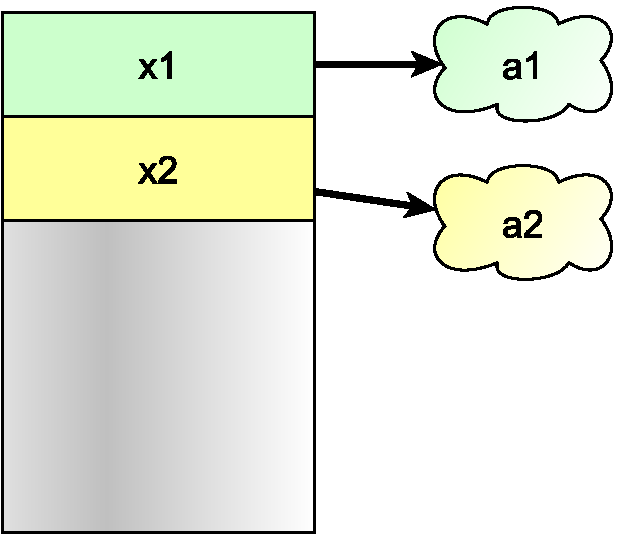
\includegraphics[width=0.6\textwidth]{illustrations/allocs-local-crop.pdf}
\caption{Помещение в вектор двух строк с локальными аллокаторами}
\label{fig:allocs_local}
\end{figure}

Пока что всё выглядит отлично: в одном векторе живут два элемента, каждый на своей позиции и каждый со своим локлаьным аллокатором.

Увы, следующий крайне простой трюк усложняет вещи совершенно непропорционально.

\begin{lstlisting}
vec.insert(vec.begin(), x3);
\end{lstlisting}

Что происходит при выполнении этой строчки? Сначала все элементы должны быть сдвинуты вниз. Первым сдвигается x2 и заводит на новом месте свой аллокатор. За ним вниз ползёт x1, но в ячейке 2 уже есть аллокатор от x2 и он там остаётся. Далее x3 помещается в ячейку 1, где работает аллокатор для 1.

На итоговой картинке (рис. \ref{fig:allocs_scope}) получается довольно устрашающая картина.

\begin{figure}[ht]
\centering
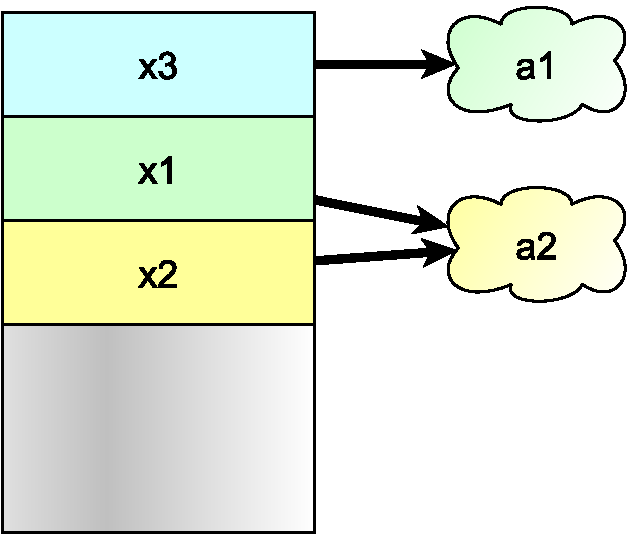
\includegraphics[width=0.6\textwidth]{illustrations/allocs-scope-crop.pdf}
\caption{Иллюстрация проблем локальных аллокаторов}
\label{fig:allocs_scope}
\end{figure}

Почему так получилось? До некоторой степени мы вообще не хотели бы чтобы строки тащили в ячейки вектора собственные аллокаторы: будет вполне достаточно если они воспользуются аллокатором вектора.

Но для этого вектор должен уметь сообщать каждой помещаемой в него строке, что у него есть свой аллокатор которым она должна пользоваться. Говорят, что у вектора должен быть распространяемый (scoped) аллокатор. Тут есть небольшая омонимия, так как на английском языке scope также означает область видимости.

Для этих целей, служит шаблон \lstinline!scoped_allocator_adapter! в стандарте C++11.

Ниже приведён пример того, как это работает для случае близкого к рассмотренному.

\begin{lstlisting}
namespace cust 
{
  template <typename T> CustomAlloc;
  template <typename T> using alloc =
     ::std::scoped_allocator_adapter<CustomAlloc<T>>;
  template <typename T> using vector = ::std::vector<T, alloc<T>>;
  template <typename T> using string = 
     ::std::basic_string<char, char_traits<char>, alloc<char>>;
}

cust::vector<cust::string> vs(&alloc1); // propagated ok
\end{lstlisting}

Теперь аллокаторы правильно пропагируются, но поглядите на этот код ещё раз. Он чудовищен. Он не может нравиться эстетически, к нему можно только привыкнуть.

Даже для обычных аллокаторов тотальное загрязнение кода вирусными шаблонами заставляет глаза кровоточить даже у опытных разработчиков.

\begin{lstlisting}
map <int, float, less<int>, s_alloc<pair<const int, float>>> m;
basic_string<char, char_traits<char>, s_alloc<char>> s;
\end{lstlisting}

Но самый убийственный аргумент против аллокаторов, обладающих состоянием это аргумент от сложности написания контейнера, корректно поддерживающего произвольные аллокаторы.

Вот достаточно условное перемещающее присваивание контейнера такого рода. Это песвдокод. В реальности проверки POCMA и IAE будут выглядеть как объяснялось выше (см. \ref{sub:freelist}).

\begin{lstlisting}
container& operator= (constainer &&rhs) {
  if (alloc_traits::POCMA) {
    clear_and_deallocate_memory();
    alloc_ = move(rhs.alloc_);
    impl_ = move(rhs.impl_);
  }
  else if (alloc_traits::IAE || alloc_ == rhs.alloc_) {
    clear_and_deallocate_memory();
    impl_ = move(rhs.impl_);
  }
  else {
    this->assign(move_iterator(rhs.begin()), 
                 move_iterator(rhs.end());
  }
  return *this
}
\end{lstlisting}

Здесь написано следующее:

\begin{enumerate}
\item Если аллокатор пропагируется на перемещающем присваивании, то достаточно обычного перемещения контейнера и перемещения аллокатора на новое место.
\item Иначе, если аллокатор сравним на равенство и оказался равным аллокатору справа, то достаточно перемещения контейнера
\item Иначе мы должны провести дорогое копирование содержимого
\end{enumerate}

По этой причине написание поддерживающего аллокаторы контейнера в реалиях C++11 это крайне интересная тема, но здесь она рассматриваться не будет, потому что, с точки зрения автора, гуманнее включённый миксер в глаза засунуть.

Причём вроде бы на пути к этому ужасу, всё было сделано правильно и логично. Это значит, что неправильный поворот был пройден довольно рано.

Вполне возможно, следует откатится к самому раннему решению: а почему вообще все исходно начали считать, что тип аллокатора должен быть частью типа контейнера?

Допустим аллокатор вообще не должен быть частью типа контейнера. В этом случае он должен быть всегда scoped и никогда не должен копироваться и перемещаться. И это приводит к идее, полноценно реализованной в C++17: идее полиморфного аллокатора.

\subsection{Полиморфные аллокаторы}\label{sub:polyalloc}

Когда в самом начале главы (см. \ref{sub:stateless}) рассматривался возможный дизайн наивного аллокатора, он был спроектирован довольно простым образом

\begin{lstlisting}
template<typename T>
struct memory_resource {
  T* allocate (size_t n);
  void deallocate(T* p, size_t n);
};
\end{lstlisting}

Пока что не следует обращать внимание на то, что я изменил название, скоро это получит своё объяснение. 

Что будет, если из этого кода удалить типы?

\begin{lstlisting}
struct memory_resource {
  virtual void* allocate (size_t n, 
    size_t align = alignof(std::max_align_t)) = 0;
  virtual void deallocate(void* p, size_t n) = 0;
  virtual bool is_equal(const memory_resource&) const = 0;
};
\end{lstlisting}

Время показало, что также очень полезной функцией для аллокаторов является проверка на равенство, поэтому она здесь добавлена.

Но в целом проектирование тут не слишком удачное, потому что параметр по умолчанию в виртуальной функции это очень нехорошо. Он свяжется статически, а не динамически и породит массу проблем, описанных ранее (см. \ref{DefArguments}).

Выходом тут является идиома NVI (см. \ref{NVI})

\begin{lstlisting}
struct memory_resource {
  void* allocate(size_t n, size_t align = alignof(max_align_t));
  void deallocate(void* p, size_t n);
  bool is_equal(const memory_resource&) const noexcept;
protected:
  virtual void* do_allocate(size_t n, size_t align) = 0;
  virtual void do_deallocate(void* p, size_t n) = 0;
  virtual bool do_is_equal(const memory_resource&) const noexcept = 0;
};
\end{lstlisting}

Получившийся класс не является аллокатором, потому что теперь он не удовлетворяет требованиям 2011-го года к интерфейсу аллокатора. Но вся прелесть в том, что он и \textbf{не называется} аллокатором. Это полиморфный ресурс в памяти, от которого теперь можно наследовать всякие интересные ресурсы.

В стандарте прописаны следующие стандартные наследники

\begin{itemize}
\item \lstinline!null_memory_resource! – самый интересный ресурс, всегда nullptr
\item \lstinline!new_delete_resource! – стандартный ресурс с new/delete
\item \lstinline!synchronize_pool_resource! – мультипул с многопоточной синхронизацией
\item \lstinline!unsynchronize_pool_resource! – быстрый мультипул без синхронизации
\item \lstinline!monotonic_buffer_resource! – монтонное выделение
\end{itemize}

Тут встречаются два новых термина – мультипул (multipool) и монотонное (monotonic) выделение. Это две стратегии работы с памятью, настолько себя зарекомендовавшие, что их предложили в стандарт. Монотонный ресурс это ресурс, который монотонно выделяет память внутри некоего заранее выделенного буфера. Память не освобождается, в конце работы прибивается сам буфер (стоит памяти при частых аллокациях). Мультипул ресурс это несколько связанных пулов, в которые выделяется и освобождается память. Пулы преаллоцируются и при нехватке, выделяется больший и больший (ускоряет работу при аллокациях/деаллокациях)

Теперь, при наличии ресурса, осталось только сделать к нему адаптер, который является честным C++11 аллокатором.

\begin{lstlisting}
template<typename T> struct polymorphic_allocator {
  polymorphic_allocator();
  polymorphic_allocator(memory_resource *mr);
  T* allocate (size_t n);
  void deallocate(T* p, size_t n);
  // .... etc ....
private: 
  memory_resource* mr_;
};
\end{lstlisting}

Выше приведён псевдокод, потому что настоящий \lstinline!polymorphic_allocator! должен быть всегда scoped, то есть наследовать от \lstinline!scoped_allocator_adaptor!.

\textbf{Вопрос к студентам:} как бы вы реализовали копирующее присваивание для \lstinline!polymorphic_allocator!?

\ifanswers
Правильный ответ: тривиально запретить. Он же ограничен по области распространения и значит привязан к месту, а не к объекту.

Более тонкий вопрос тут что делать с конструктором копирования. На удивление самым разумным выбором будет оставить его по умолчанию, то есть копировать значение указателя на \lstinline!memory_resource! по значению. Приходите на мои лекции, там я разбираю ходы в этой позиции и показываю к чему приводят все остальные. Или сделайте это дома сами, тут не высшая математика, тут всё просто.
\fi

Начиная с C++17, вся стандартная библиотека с полиморфной аллокацией включена в пространство имён \lstinline!std::pmr!.

\begin{lstlisting}
namespace pmr {
  template <class T> using vector =
    ::std::vector<T, std::pmr::polymorphic_allocator<T>>;
  // .... all other containers ....
}
\end{lstlisting}

Для удобства туда же включены классы полиморфного аллокатора, основные ресурсы в памяти и прочее.

Следующий код это пример ещё одного вектора на стеке, на этот раз в реалиях pmr.

\begin{lstlisting}
constexpr size_t sz = 1000 * sizeof(double);
char buffer[sz] alignas(double);
pmr::monotonic_buffer_resource alloc(buffer, sz);
double start = 0.0;
pmr::vector<double> v1(&alloc);
generate_n(back_inserter(v1), 100, 
  [start] () mutable { return (start += 1.1); });
\end{lstlisting}

Здесь прекрасно всё, но особенно то, что вообще нет аллокаций в динамическую память.

Иногда стандартных ресурсов недостаточно и хочется написать свой ресурс, который инкапсулировал бы свою уникальную стратегию распределения памяти.

\subsection{Иерархия ресурсов в памяти}\label{sub:testresrc}

Для примера можно разработать тестовый ресурс. Он проверяет что аллокация соответствует деаллокации и пытается отслеживать утечки памяти.

\begin{lstlisting}
struct test_resource : public pmr::memory_resource {
  // interface here
private:
  struct allocation_rec {
    void *ptr_;
    size_t nbytes_, nalign_;
  };
  pmr::memory_resource *parent_;
  pmr::vector<allocation_rec> blocks_;
};
\end{lstlisting}

Переопределение \lstinline!do_allocate!

\begin{lstlisting}
void *test_resource::do_allocate(size_t bytes, size_t align) {
  void *ret = parent_->allocate(bytes, align);
  blocks_.emplace_back(ret, bytes, align);
  return ret;
}
\end{lstlisting}

Видно, что тестовый ресурс просто сцепляется с тем, над которым он живёт. Это обычная идея: теперь можно складывать \lstinline!memory_resources! в иерархические стопки.

Но любая иерархия неизбежно порождает вопрос, кто в этой иерархии находится сверху.

\begin{lstlisting}
static test_resource newdefault{pmr::new_delete_resource()};
pmr::set_default_resource(&newdefault);
\end{lstlisting}

Для установки ресурса по умолчанию для pmr контейнеров, в стандарте был оставлен хук \lstinline!pmr::set_default_resource! и это худшее, что там было оставлено. Простейший способ нарваться на проблемы тут, это, например, забыть слово \lstinline!static!.

\textbf{Вопрос к студентам:} кстати, а что будет, если тут забыть слово \lstinline!static!?

\ifanswers
Правильный ответ: проблемы при выполнении деструкторов объектов, которые будут закладываться на то, что дефолтный ресурс ещё существует.
\fi

Итак, начиная с 2017 года, собственных аллокаторов писать вообще не надо, так как полиморфного аллокатора хватит на всех, а собственные ресурсы в памяти писать действительно просто. Что насчёт собственных контейнеров? Конечно их тоже стало писать удивительно просто.

\subsection{Собственные контейнеры, пользующиеся аллокаторами}\label{sub:polycont}

Для примера подобного рода контейнера можно взять что-то, чего нет в стандарте. В докладе господина Халперна на CppCon \cite{talk:halpern:allocators} рассматривался альтернативный дизайн односвязного списка, поддерживающего быстрый \lstinline!size! ценой медленного \lstinline!splice! и быструю вставку как в хвост, так и в голову. Принципиальное устройство такого списка показано на (рис. \ref{fig:slist}). 

\begin{figure}[ht]
\centering
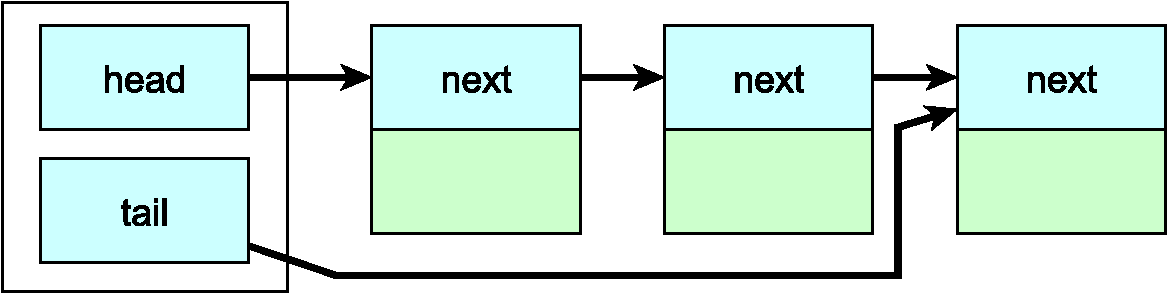
\includegraphics[width=0.6\textwidth]{illustrations/slist-crop.pdf}
\caption{Альтернативный односвязный список}
\label{fig:slist}
\end{figure}

Как может быть утсроен узел для такого контейнера? Очевидная для программиста с первого взгляда схема на листинге ниже имеет один недостаток.

\begin{lstlisting}
template <typename Tp> struct node;
template <typename Tp> struct node_base {
  node<Tp> *next_ = nullptr;
  node_base(const node_base&) = delete;
  node_base& operator=(const node_base&) = delete;
};
template <typename Tp> struct node : node_base<Tp> {
  Tp value_;
};
\end{lstlisting}

Недостаток тут в том, что сложно придумать разумное значение по умолчанию для \lstinline!value_!. Оно будет инициализировано при конструировании но чем и зачем -- неясно.

Выход в распространённом трюке, использующем union: начиная с 2011 года объединения в C++ могут объединять нетривиальные объекты с учётом, что пользователь сам заботится об их памяти.

\begin{lstlisting}
template <typename Tp> struct node : node_base<Tp> {
  union { Tp value_; };
};
\end{lstlisting}

Это улучшение позволяет внести немного неочевидной job security в код и, одновременно, сэкономить пару тактов времени исполнения (но последнее не точно). Какой же C++ разработчик удержится.

Скелет для итогового класса списка с некоторыми важными частями внутри приведён ниже.

\begin{lstlisting}
template <typename T> struct slist { 
  using value_type = T;
  using allocator_type = pmr::polymorphic_allocator<byte>;
  // .... etc ....
public:
  slist(allocator_type a = {}) : 
    head_{}, ptail_{&head_}, size_{0}, alloc_{a} {};
  allocator_type get_allocator() const { return alloc_; }
  // .... etc ....
private:
  node_base head_;
  node_base *ptail_;
  size_t size_;
  allocator_type alloc_;
};
\end{lstlisting}

Тот факт, что список способен пользоваться произвольным полиморфным аллокатором, здесь считывается из двух обязательных пунктов:

\begin{enumerate}
\item Наличия зависимого типа \lstinline!allocator_type!
\item Наличия метода \lstinline!get_allocator! 
\end{enumerate}

Тип \lstinline!polymorphic_allocator<byte>! здесь это как бы общий базовый класс для всех аллокаторов. В принципе содержимое треугольных скобок у него не слишком важно: при наличии ребинда, какая разница для какого он типа. Это всего лишь тяжёлое легаси интерфейса 1998-го года.

Удивительное наблюдение тут состоит в том, что все составляющие хороших и правильных аллокаторов уже были известны в 98-м году, но люди стремились к шаблонной сложности и получили её. Урок состоит к том, что хороший программист стремится не к сложности, а к простоте.

Ключевым методом контейнера \lstinline!slist!, разумеется, является \lstinline!emplace!, поскольку именно в его терминах будет реализована вся остальная вставка.

Скелет правильного создания 

\begin{lstlisting}
template <typename ... Args> iterator
emplace (iterator i, Args&& ... args) {
  void *mem = alloc_.resource()->allocate(sizeof(node), alignof(node));
  node *ret = static_cast<node*>(mem);
  ret->next_ = i.prev->next_;
  alloc_.construct(addressof(ret->value_), forward<Args>(args)...);
  i.prev->next_ = ret;
  // .... some corner cases .... 
}
\end{lstlisting}

\textbf{Вопрос к студентам}: кто видит проблему в этом коде?

\ifanswers
Правильный ответ: разумеется она в безопасности исключений. Конкретно исключение с самыми печальными последствиями может прилететь из \lstinline!construct!
\fi

\subsection{Сводная таблица}\label{sub:taballoc}

Аллокаторы это такой своеобразный и так часто меняющшийся механизм стандартной библиотеки, что в нём ничего не стоит запутаться.

Будут ли они меняться дальше или придуманные в 2017 году полиморфные аллокаторы совершенны? Скорее всего, ещё несколько итераций изменения неизбежны. Простейший аргумент это аргумент от стоимости поддержки.

Представьте обычную структуру, состоящую из целого числа и вектора. 

\begin{lstlisting}
struct S {  
  int n;
  vector<int> v;
}; 
\end{lstlisting}

Сейчас, так как она написана, эта структура имеет по умолчанию всё необходимое: копирование, присваивание, всё остальное. Кроме поддержки аллокаторов. Сколько кода надо написать, чтобы завести в ней эту поддержку? Увы, даже сейчас это тонны кода. Но чисто интуитивно в этом случае (вектор плюс один элемент) поддержка не должна стоить ничего: вектор уже всё поддержал и завести ещё одно целое под этот зонтик -- технический момент.

Для простоты отслеживания, изменения сложности простейших задач (в весьма условных попугаях) сведены в таблицу.

\begin{center}
\begin{tabular}{ | l | l | l | l | }
  \hline
  Task &  C++98 & C++11 & C++17 \\ \hline \hline
  Использование & MEDIUM & MEDIUM & EASY \\ \hline 
  Создание & MEDIUM & EASY & EASY \\ \hline
  Создание stateful &  IMPOSSIBLE & EASY & EASY \\ \hline 
  Создание scoped & IMPOSSIBLE & MEDIUM & EASY \\ \hline
  Новый контейнер & MEDIUM & HARD & MEDIUM \\ \hline
  \hline
\end{tabular}
\end{center}

Это завершает обсуждение аллокаторов.

\pagebreak
\section{Концепты\index{Concepts}}\label{Concepts}

\hfill\textit{Thoughts without content are empty,}

\hfill\textit{intuitions without concepts are blind}{\vspace{0.5em}}

\hfill\textit{-- Immanuel Kant}

Любую компьютерную программу читает (и иногда пишет) разработчик, который оперирует семантическим смыслом выражений языка программирования. При этом у разработчика есть очень большое количество корректных синтаксических форм для семантически эквивалентных конструкций.

Но ту же программу читает (обрабатывает) компилятор, который не понимает её смысла. Вместо этого компилятор механически упрощает выражения и трансформирует их, ориентируясь на их финальное представление в целевой архитектуре. Так выражению имеющему смысл сложения величин могут быть сопоставлены принципиально разные инструкции ассемблера в зависимости от того являются эти числа целыми или с плавающей точкой.

Именно тот факт, что смысл выражений высокоуровневых языков часто совершенно не зависит от типов и конкретной интерпретации этих выражений, позволяет обобщенное программирование как таковое.

Почти классический пример обобщенного кода: функция для нахождения элемента в диапазоне (диапазон здесь может быть вектором, списком, декой, множеством, пользовательским типом, согласующимся с сокращенным синтаксисом \lstinline!for!). Это (а также тип элемента) серьёзно повлияет на конкретный сгенерированный код, но совсем не повлияет на смысл следующей простой конструкции:

\begin{lstlisting}
template<typename R, typename T> bool 
in (R const& range, T const& value) 
{
  for (auto const& x : range)
    if (x == value)
      return true;
  return false;
}
\end{lstlisting}

\textbf{Вопрос к студентам}: что будет при попытке использовать этот код неправильно, например ``найти'' число в векторе строк?

\begin{lstlisting}
vector<string> v { "0", "1", "2" };
bool is_in = in (v, 0);
\end{lstlisting}

%\ifanswers
Очевидно ошибка компиляции. Главная проблема в том, что это будет \textbf{неприятная} ошибка компиляции:

\begin{verbatim}
In file included from /home/tilir/Applications/gcc-5.2/include
/c++/5.2.0/bits/stl_algobase.h:67:0,
                 from /home/tilir/Applications/gcc-5.2/include
/c++/5.2.0/vector:60,
                 from constr1.cc:1:
/home/tilir/Applications/gcc-5.2/include/c++/5.2.0/bits
/stl_iterator.h:820:5: note: candidate: 
template<class _IteratorL, class _IteratorR, class _Container> 
bool __gnu_cxx::operator==(const __gnu_cxx::__normal_iterator
<_IteratorL, _Container>&, const __gnu_cxx::__normal_iterator
<_IteratorR, _Container>&)
     operator==(const __normal_iterator
<_IteratorL, _Container>& __lhs,
     ^
/home/tilir/Applications/gcc-5.2/include/c++/5.2.0/bits
/stl_iterator.h:820:5: note:   template argument deduction
/substitution failed:
constr1.cc:10:11: note: ‘const std::__cxx11::basic_string<char>’ 
is not derived from ‘const __gnu_cxx::__normal_iterator
<_IteratorL, _Container>’
     if (x == value)
\end{verbatim}

Это только крошечный кусочек из простыни которую выдаст gcc-5.2
%\fi

\textbf{Домашняя наработка:} попробуйте скомпилировать ещё более простой код:

\begin{lstlisting}
class X {};
std::set<X> x;
x.insert(X{});
\end{lstlisting}

В своё время обобщенное программирование на C++ сильно споткнулось об это. Эти знаменитые простыни ошибок, которые заставляли даже опытных разработчиков кричать и плакать как детей, увы, неизбежны. Шаблоны добавляют лишний шаг к компиляции программы: сначала должны быть инстанциированы типы, потом скомпилирован код. В случае если инстанцирование создало большой стек, будет много ошибок, без рациональной возможности сократить их, если нет механизмов ограничить шаблонный полиморфизм и заблокировать собственно инстанцирование. Между прочим, безо всякого шаблонного инстанцирования точно таких же безумных ошибок можно добиться макросами.

\begin{lstlisting}
#include __FILE__
p;
\end{lstlisting}

Идея здесь та же -- макроподстановка никак не ограничена. Но макроподстановка не Тьюринг полна, поэтому в макросах это менее актуально (там обычно просто нет достаточно большого стека подстановки чтобы развернуться). Хотя если кто-то хоть раз пробовал boost preprocessor, он знает боль. А в шаблонах рекурсивные вызовы -- обычное дело. И тем важнее добиться того, чтоб неправильные ветки отсекались как можно раньше.

Итак ключ к обоснованию нововведений в языке и главная тема этой лекции: \textbf{ограничение шаблонного полиморфизма}.

Ограничить шаблонный полиморфизм -- также хорошая идея для разделения типов: иногда хотелось бы такой обобщенный тип, который ведет себя по разному когда инстанцирован чем-то вроде целого или чем-то вроде плавающего числа (может быть даже имеет разные методы).

Итак, ограничений и контроля полиморфизма в языке явно не хватало. И, конечно, все всегда понимали, что с этим надо что-то делать. За много лет коммьюнити наработало некий опыт.

\subsection{Добрые старые способы контроля полиморфизма}

В этом разделе будут рассмотрены методы, работающие для C++14. Поскольку это часто связано с написанием большого количества кода, лучше в качестве рабочего примера рассмотреть очень простую обобщенную функцию проверки значений двух разных типов на равенство.

\begin{lstlisting}
template <typename T, typename U> bool
check_eq (T &&lhs, U &&rhs) {
  return (lhs == rhs);
}
\end{lstlisting}

Её также можно использовать правильно или ошибочно.

\begin{lstlisting}
// no operator ==  here
struct noeq {
  noeq (int x) {}
};

int main () {
  check_eq (1, 1);       // ok
  check_eq (1, 1.0);     // ok
  check_eq (1, noeq(1)); // problems
  return 0;
}
\end{lstlisting}

В случае ошибочного использования, ошибка компиляции выглядит очень простой:

\begin{verbatim}
eqcomp00.cc: In instantiation of 
  ‘bool check(T&&, U&&) [with T = int; U = noeq]’:
eqcomp00.cc:13:20:   required from here
eqcomp00.cc:3:15: error: no match for 
  ‘operator==’ (operand types are ‘int’ and ‘noeq’)
   return (lhs == rhs);
\end{verbatim}

Но, тем не менее, хотелось бы вместо неё иметь нечто осмысленное.

Простейший способ, и, обычно, первый, который приходит в голову новичку, это влепить статическую проверку.

\begin{lstlisting}
static_assert (is_equality_comparable<T, U>::value, 
              "Comparable types required");
\end{lstlisting}

Для этого надо сначала понять, что такое \lstinline!is_equality_comparable!. В стандарте C++14 ничего такого нет, но хороший программист без труда спляшет это ограничение на SFINAE в C++14.

\begin{lstlisting}
template <typename T, typename U, typename = void>
struct is_equality_comparable : std::false_type {};

// I feel really C++ here
template <typename T, typename U>
struct is_equality_comparable <T, U,
    decltype ((void)(std::declval<T&>() == std::declval<U&>()))
  > : std::true_type {};
\end{lstlisting}

Стало ли лучше?

\begin{verbatim}
eqcomp00.cc: In instantiation of 
  ‘bool check(T&&, U&&) [with T = int; U = noeq]’:
eqcomp00.cc:28:27:   required from here
eqcomp00.cc:16:3: error: static assertion failed: 
   Comparable types required
   static_assert (is_equality_comparable<T, U>::value, 
   ^
eqcomp00.cc:18:15: error: no match for 
   ‘operator==’ (operand types are ‘int’ and ‘noeq’)
   return (lhs == rhs);
\end{verbatim}

Стало хуже. Мы получили static assertion failure и, \textbf{вдобавок} к нему, также instantiation failure.

Проблема в том, что эти ошибки проявляются \textbf{поздно}. Компилятор уже начал инстанцирование шаблона и он уже прошел по этому пути достаточно далеко. Наличие или отсутствие failures далее ничего не значат. Таким образом, \lstinline!static_assert! в языке нужен не для этого. Он не мешает компилятору разобрать функцию, а защищает от ошибок, которые вызваны несовпадением статических контрактов.

Гораздо интереснее использовать \lstinline!enable_if!, который даёт возможность выбросить функцию из рассмотрения:

\begin{lstlisting}
// Wow, I am even MORE C++ now
template <typename T, typename U,
          typename = std::enable_if_t <
             is_equality_comparable<T, U>::value>
          >
bool check (T &&lhs, U &&rhs);
\end{lstlisting}

В \lstinline!enable_if<false, T>! нет зависимого типа \lstinline!enable_if<false, T>::type! и происходит классический случай SFINAE, см. (\ref{SFINAE}).

Ошибка выглядит более вразумительно:

\begin{verbatim}
eqcomp01.cc:27:20: error: 
  no matching function for call to ‘check(int, noeq)’
   check (1, noeq(1));

eqcomp01.cc:18:6: note: candidate: 
  template<class T, class U, class> bool check(T&&, U&&)
  bool check (T &&lhs, U &&rhs);
       ^
eqcomp01.cc:18:6: note:   
  template argument deduction/substitution failed
\end{verbatim}

Инстанцирования такой функции просто не происходит. Тем не менее, сложно не заметить, что синтаксис для вышивания на \lstinline!enable_if! переусложнен и требует для блокирования подстановки завязываться на третий шаблонный параметр, который в общем не при чём.

\subsection{Простые ограничения\index{Constraints}}\label{Constraints}

Введение в новый стандарт синтаксического сахара для таких конструкций было практически неизбежным.

\begin{lstlisting}
template <typename T, typename U>
requires is_equality_comparable<T, U>::value
bool check (T &&lhs, U &&rhs);
\end{lstlisting}

Теперь правильное использование всё так же идёт без ошибок. В то же время неправильное использование выдает простую ошибку:

\begin{verbatim}
eqcomp01s.cc: In function ‘int main()’:
eqcomp01s.cc:27:20: error: cannot call function 
  ‘bool check(T&&, U&&) [with T = int; U = noeq]’
   check (1, noeq(1));
                    ^
eqcomp01s.cc:18:6: note:   constraints not satisfied
 bool check (T &&lhs, U &&rhs);
      ^~~~~
eqcomp01s.cc:18:6: note:   
   ‘is_equality_comparable<T, U>::value’ evaluated to false
\end{verbatim}

Главное в этой ошибке то, что она, как и в случае \lstinline!enable_if!, выдается \textbf{рано}, то есть задолго до того, как компилятор реально полез инстанцировать что бы то ни было. Sutton сообщал об уменьшении времени компиляции хорошо ограниченного таким образом кода на десятки процентов.

Явная запись \lstinline!requires! в таком контексте называется ограничением (constraint) и в данном случае использует для проверки ограничения функцию стандартной библиотеки.

Также это является \textit{requires-clause} -- собственно ограничением. Немного позже будут введены \textit{requires-expressions} -- то, что будет называться ограничивающими выражениями. Уже сейчас хочется предупредить, что их нельзя путать.

Несмотря на то, что в этом разделе ограничения вводятся как ограничения для обобщенного программирования, на самом деле в них нет ничего магического: это обычный C++ и они могут использоваться с обычными функциями.

\begin{lstlisting}
void f ()
requires sizeof(int) == 4
{
 /* do something */
}
\end{lstlisting}

И даже более того, нешаблонные функции могут быть ограничены охватывающими шаблонными параметрами.

\begin{lstlisting}
template <typename T>
class vector {
  // ....
  // we have copy ctor only if T copyable
  requires std::is_copyable<T>::value
  vector (const vector&);
};
\end{lstlisting}

\textbf{Домашняя наработка:} попробуйте такое сделать на \lstinline!enable_if! просто чтобы понять масштаб упрощения.

Констрейнты работают лениво: возможное нарушение размера целого будет проверено только в точке вызова этой функции. Нет вызова -- нет проблем.

\textbf{Вопрос к студентам:} кстати об ограничениях на ограничения. А как вы думаете, виртуальные функции могут быть ограничены подобным образом?

\ifanswers
Правильный ответ: конечно не могут (примерно по тем же причинам, по каким они не могут быть шаблонными). В таблице виртуальных функций просто нет места для этого признака, а связывать его со статическим типом чревато проблемами.
\fi

\subsection{Пример -- перегрузка конструкторов}

Во многих случаях даже простых констрейнтов достаточно, чтобы чудесно упрощать код. Типичная задача -- внутри обобщенного класса иметь отдельно конструктор из плавающих и отдельно из целочисленных типов (пример взят из доклада Роджера Орра на ACCU 2016). 

Если решать эту задачу на бумажке, на ум приходит решение в старом добром стиле.

\begin{lstlisting}
struct Foo {
  enum {int_like, float_like} type_;

  template <typename Int, 
            typename = std::enable_if_t<
              std::is_integral<Int>::value>
            >
  Foo (Int x) : type_(int_like) { 
    std::cout << "int like: " << x; 
  }

  template <typename Float, 
            typename = std::enable_if_t<
              std::is_floating_point<Float>::value>
            >
  Foo (Float x) : type_(float_like)  { 
    std::cout << "float like: " << x; 
  }
};

int main () {
  Foo (1);
  Foo (5.0);
  return 1;
}
\end{lstlisting}

Увы, у него есть небольшой недостаток -- оно не скомпилируется.

\begin{verbatim}
ctorex01.cc:13:3: error: 
  ‘template<class Float, class> Foo::Foo(Float)’ 
   Foo (Float x) : type_(float_like)     
   ^~~
ctorex01.cc:9:3: error: with 
  ‘template<class Int, class> Foo::Foo(Int)’
   Foo (Int x) : type_(int_like)
\end{verbatim}

Шаблонные функции просто не могут быть перегружены по имени шаблонного параметра. Впрочем, танки грязи не боятся и немного времени в отладчике приводит к более интересному решению.

\begin{lstlisting}
struct Foo {

  enum {int_like, float_like} type_;

  template <int> struct dummy { dummy(int) {} };

  template <typename Int,
            typename = std::enable_if_t<
              std::is_integral<Int>::value>
            >
  Foo (Int x, dummy<0> = 0) : type_(int_like)
  {
    std::cout << "int like: " << x << std::endl;
  }

  template <typename Float,
            typename = std::enable_if_t<
              std::is_floating_point<Float>::value>
            >
  Foo (Float x, dummy<1> = 0) : type_(float_like)
  {
    std::cout << "float like: " << x << std::endl;
  }
};
\end{lstlisting}

Теперь все хорошо, но опять ценой некоторой избыточности. В то же время даже с самыми простыми ограничениями та же задача решается как персик.

\begin{lstlisting}
struct Foo {

  enum {int_like, float_like} type_;

  template <typename Int>
  requires std::is_integral<Int>::value
  Foo (Int x) : type_(int_like)
  {
    std::cout << "int like: " << x << std::endl;
  }

  template <typename Float>
  requires std::is_floating_point<Float>::value
  Foo (Float x) : type_(float_like)
  {
    std::cout << "float like: " << x << std::endl;
  }

};
\end{lstlisting}

Со скромной точки зрения автора, даже если бы ограничения ввели только в виде простых ограничений, это серьёзно разгрузило бы метапрограммирование во многих практически важных контекстах.

\subsection{Сложные ограничения}

Простыми ограничениями можно написать три вида выражений: предикаты, конъюнкции предикатов и дизъюнкции предикатов.

\textbf{Вопрос к студентам:} пусть задан предикат:

\begin{lstlisting}
template <typename T>
constexpr int somepred() {
  return 14;
}
\end{lstlisting}

выполняются или нет указанные констрейнты для функции \lstinline!check! если первый терм ложен?

\begin{lstlisting}
template <typename T, typename U>
requires is_equality_comparable<T, U>::value &&
         (somepred<T>() == 14) || 
         (somepred<U>() == 42)
bool check (T &&lhs, U &&rhs);
\end{lstlisting}

\ifanswers
Правильный ответ: конечно нет, так как \lstinline!false && true || false! по обычной схеме дает false
\fi

К сожалению, это не всё, что может быть нужно от ограничений. Простой пример: как избавиться от всё ещё необходимого шаблонного определения \lstinline!is_equality_comparable!? Для этого может быть использовано сложное ограничение, использующее ограничивающие выражения (requires-expressions).

\begin{lstlisting}
template <typename T, typename U>
requires requires(T t, U u) { t == u; }
bool check (T&& lhs, U&& rhs);
\end{lstlisting}

Ключевое слово \lstinline!requires! упомянутое дважды делает именно это -- открывает ограничение, после чего вместо предиката использует в нем ограничивающее выражение.

Ограничивающие выражения похожи на константно-выраженные (constexpr) функции. Но в них есть своя магия. Она заключается в том, что сложные ограничения никогда не вычисляются, в этом они похожи на выражения-параметры decltype. Для них только проверяются типы. Это создаёт громадную разницу между двумя формами ограничений

\begin{lstlisting}
// (1) constexpr function somepred ct evaluated
template <typename T>
requires somepred<T>() == 42
bool foo (T&& lhs, U&& rhs);

// (2) constexpr function somepred typechecked only
template <typename T>
requires requires (T t) { 
  somepred<T>() == 42;
}
bool bar (T&& lhs, U&& rhs);
\end{lstlisting}

Именно это делает сложные ограничения сложными.

Есть три основных категории сложных ограничивающих выражений:

\begin{enumerate}
\item Базовые ограничивающие выражения -- проверяют наличие операции над типами и на этом всё.

\begin{lstlisting}
template <typename T>
requires requires (T a, T b) {
           a + b;
         }
T test1 (T, T);
\end{lstlisting}

Есть некое тонкое различие между simple и expression requirements, выше указана первая форма, но это уже очень тонкая разница.

\item Ограничивающие выражения для типов -- проверяют наличие типа.

\begin{lstlisting}
template <typename T>
requires requires() {
           typename T::inner;
         }
T test2 (T, T);
\end{lstlisting}

\item Составные ограничивающие выражения -- проверяют и операцию и выводимый тип.

\begin{lstlisting}
template <typename T>
requires requires(T x) {
           {*x} -> typename T::inner;
         }
T test3 (T, T);
\end{lstlisting}

\end{enumerate}

Кроме этих ограничений есть ещё ограничения на спецификацию исключений и прочая экзотика, которую можно прочитать в очередном TS, но чтобы составить общее впечатление достаточно различать эти три вида.

Немножко практики. Пусть даны структуры, отвечающие некоторым из упомянутых выше требований.

\begin{lstlisting}
struct HasInner {
  using inner = int;
};

struct HasDeref {
  using inner = int;
  inner operator*();
};
\end{lstlisting}

Можно посмотреть какие выполняются и не выполняются в каких случаях.

\begin{lstlisting}
int main () {
  test1(1, 1);
  test1(HasInner{}, HasInner{}); // no +
  test2(HasInner{}, HasInner{});
  test2(1, 1); // no inner
  test3(HasDeref{}, HasDeref{});
  test3(HasInner{}, HasInner{}); // no deref
}
\end{lstlisting}

Разумеется сложные ограничивающие выражения можно комбинировать.

\begin{lstlisting}
template <typename T>
requires requires(T x) {
           {*x} -> typename T::inner;
         } &&
         requires() {
           typename T::inner;
         } &&
         requires (T a, T b) {
           a + b;
         }
T test4 (T, T);
\end{lstlisting}

\textbf{Вопрос к студентам:} написать тип, который подойдет под такое ограничение.

\ifanswers
Вариант ответа:
\begin{lstlisting}
struct HasPlus {
  using inner = int;
  inner operator*();
  void operator+(HasPlus x);
};
\end{lstlisting}
\fi

Сложные ограничения позволяют очень многое (неожиданно многое) но они имеют несколько сложный синтаксис, поэтому сложные примеры следует отложить до введения простого способа выносить сложные ограничения в общую часть -- собственно концептов (мы до них добрались, да).

\subsection{Простые концепты}

Выше уже можно было увидеть, что сложные ограничения могут быть очень сложны, а главное -- всегда есть желание их переиспользовать, а не писать каждый раз заново.

Например можно прикинуть какой интерфейс должен поддерживать тип, чтобы быть последовательностью с обратной вставкой (Sequence)? На ум приходит следующее.

\begin{enumerate}
\item тип \lstinline!T::element_type! для указания своего типа элементов
\item метод \lstinline!size()! для проверки размера, возвращающая \lstinline!size_t!
\item метод \lstinline!empty()! для проверки пустоты, возвращающий \lstinline!bool!
\item метод \lstinline!back()! для получения последнего элемента, возвращающий \lstinline!T::element_type!
\item метод \lstinline!push_back()! для вставки в конец последовательности
\end{enumerate}

Простой концепт для такого класса типов можно определить как (это можно пошагово разобрать у доски).

\begin{lstlisting}
template <typename T>
concept bool Sequence() {
  return
    requires { typename T::element_type; } &&
    requires (T t, typename T::element_type x) {
      { t.size() } -> size_t;
      { t.empty() } -> bool;
      { t.back() } -> typename T::element_type;
      { t.push_back(x) } // not specified (!)
    };
}
\end{lstlisting}

Есть несколько форм эквивалентного синтаксиса, в которых можно использовать получившийся концепт:

\begin{enumerate}

\item Базовый синтаксис -- явное использование в ограничении 
\begin{lstlisting}
template <typename T> 
requires Sequence<T>
void fill_with_random (T &x, int n);
\end{lstlisting}

\item Упрощенный синтаксис -- вынос констрейнта в шаблонный параметр

\begin{lstlisting}
template <Sequence T> 
void fill_with_random (T &x, int n);
\end{lstlisting}

\item Синтаксис с выводом типов:

\begin{lstlisting}
void fill_with_random (Sequence &x, int n);
\end{lstlisting}

\end{enumerate}

Последний вариант выглядит несколько странно (и вызывает обоснованную критику), но в языке уже включена в стандарт C++17 возможность эквивалентно писать формы для обычных функций с шаблоном и с \lstinline!auto!.

\begin{enumerate}
\item Форма обычного шаблона функции 
\begin{lstlisting}
template <typename T> 
void foo (T x);

template<typename T, typename U, typename V> 
void bar(T (U::*)(V));
\end{lstlisting}
\item Форма с выводом типов
\begin{lstlisting}
void foo (auto x);

void bar(auto (auto::*)(auto));
\end{lstlisting}

\end{enumerate}

В свете этого идея такого же вывода концептами находится вполне в русле преобразований в язык. Аналогично в языке уже (с 14-го года) существуют обобщенные лямбды. Аналогично нет ничего противоестественного в том, чтобы ограничивать их концептами.

\begin{enumerate}
\item Обобщенная лямбда
\begin{lstlisting}
find_if(v, [str](const auto& x) 
           { return str == x; });
\end{lstlisting}
\item Ограниченная обобщенная лямбда
\begin{lstlisting}
find_if(v, [str](const String& x)
           { return str == x; });
\end{lstlisting}
\end{enumerate}

Есть некие ограничения на то, как могут быть устроены простые концепты-функции: они всегда возвращают \lstinline!bool!, никогда не принимают аргументов, состоят только из одного \lstinline!return! (похоже на старые добрые константно-выраженные функции в C++11) и не могут быть ни объявлены а позже определены, ни сделаны функциями-членами, ни быть друзьями классов. И конечно, в отличии от аргументов \lstinline!constexpr! функций, аргументы концептов не могут быть ограничены в свою очередь концептами.

Концепты (в рамках COncepts Lite) не проверяют семантику, то есть нельзя проверить, что

\begin{lstlisting}
t.empty() == (t.size() == 0)
\end{lstlisting}

Концепты также не проверяют реализацию: пользователь может заложиться внутри шаблона на неявный интерфейс не предусмотренный концептом

\begin{lstlisting}
template<Range R, typename T> bool
requires RangeEqComparable<R, T>()
in (R const& range, T const& value) {
  for (auto const& x : range)
    if (x != value) // OOPS!
      return false;
  return true;
}
\end{lstlisting}

Этот пункт вызывает споры и критику. Многие считают, что как раз проверять реализацию шаблона -- важное предназначение концептов как инструмента.

В рассмотренном выше примере, концепт \lstinline!Sequence! состоял только из сложных ограничений, но можно делать концепты и из простых ограничений.

\begin{lstlisting}
template <typename C> 
concept bool isInt() { 
  return std::is_integral<C>::value;
}
\end{lstlisting}

Мало того, концепты вообще не обязаны быть функциями. Самые простые концепты получаются из шаблонных переменных.

\begin{lstlisting}
template <typename C> 
concept bool Int = std::is_integral<C>::value;
\end{lstlisting}

Это работает так же как обычные шаблонные переменные. Можно записать даже проще.

\begin{lstlisting}
template <typename T>
concept bool Int = is_integral_v<T>;

template <typename T>
concept bool Float = is_floating_point_v<T>;
\end{lstlisting}

Здесь использован явный синтаксис присваивания концепту шаблонна переменной (по сути присваивание на метаклассах).

Увы, концепты не поддерживают рекурсию и поэтому не Тьюринг-полны. Также их нельзя специализировать. Зато возможна частичная специализация по констрейнту:

\begin{lstlisting}
template <typename T>
class complex;

template <Float T>
class complex { /* complex numbers */ };

template <Int T>
class complex { /* gaussian integers */ };
\end{lstlisting}

Это похоже на пример с конструкторами, но выглядит ещё более симпатично. Самое интересное: любой (даже тривиальный как C1 выше) констрейнт ограничивая шаблон делает его более специализированным, чем не ограниченный шаблон.

Не менее красиво выглядит теперь и пример с перегрузкой конструкторов:

\begin{lstlisting}
struct Foo {
  enum {int_like, float_like} type_;
  Foo (Int x);
  Foo (Float x);
};
\end{lstlisting}

Тем не менее, иногда нетривиальный концепт может быть довольно сложен. Поэтому простые концепты можно писать в терминах ещё более простых. Например для уже рассматривавшейся проверки на сравнимость на равенство можно соорудить вот такое:

\begin{lstlisting}
template <typename T, typename U>
concept bool Weak_equality_comparable() {
  return requires(T t, U u) {
    {t == u} -> bool;
  };
}

template <typename T, typename U = T>
concept bool Equality_comparable() {
  return Weak_equality_comparable<T, U>() &&
         Weak_equality_comparable<U, T>();
}
\end{lstlisting}

Но вот в том как воспользоваться таким концептом для определения функции \lstinline!check()! есть тонкости.

\textbf{Вопрос к студентам:} сработает ли вот такой вариант?

\begin{lstlisting}
template <Equality_comparable T,
          Equality_comparable U>
bool check(T, U);
\end{lstlisting}

\ifanswers
Он сработает, но не так как можно ожидать: будет проверено что \lstinline!T! сравнимо с \lstinline!T! и что \lstinline!U! сравнимо с \lstinline!U!. Но программист скорее всего хочет проверить, что \lstinline!T! сравнимо с \lstinline!U!.
\fi

Для решения этой задачи можно использовать либо явный синтаксис с ограничением, либо принципиально новый синтаксический выверт -- введение шаблона.

\begin{lstlisting}
Equality_comparable{T, U}
bool check(T, U);
\end{lstlisting}

Эта запись является сокращением для

\begin{lstlisting}
template <typename T, typename U>
requires Equality_comparable<T, U>()
bool check(T, U);
\end{lstlisting}

И выглядит довольно интересно. Также столь удобный синтаксис позвоялет заменить \lstinline!auto! на концепт:

\begin{lstlisting}
template <typename C> 
concept bool Int = std::is_integral<C>::value;

// ...

Int x = f(x); // auto x = f(x);
\end{lstlisting}

Благодаря концепту теперь в коде будет яснее чего ожидать от вывода типов (ну и усилится проверка от человеческих ошибок).

\subsection{Вариабельные концепты}

Ещё один пример полезного использования получившегося ограничения \lstinline!Sequence! это подсчет количества элементов, удовлетворяющих предикату. Первый вариант может выглядеть как-то так.

\begin{lstlisting}
template <Sequence S, typename P>
int count (S const& seq, P pred) {
  int n = 0;
  for (auto const &x : seq)
    if (pred(x)) ++n;
  return n;
}
\end{lstlisting}

Увы, он очевидно underconstrained (русское слово недоограничен звучит не менее ужасно). Вместо второго параметра может быть передано все что угодно. Чтобы это исправить, нужно ввести явное ограничение, например так:

\begin{lstlisting}
template <Sequence S, typename P>
  requires Predicate<P, typename S::element_type>()
int count (S const& seq, P pred) {
  int n = 0;
  for (auto const &x : seq)
    if (pred(x)) ++n;
  return n;
}
\end{lstlisting}

Но что такое \lstinline!Predicate!? Очевидно это функция, которая может быть вызвана с аргументом, заданного типа. Идея заключается в том, что аргументов может быть сколько угодно, поэтому можно воспользоваться вариабельными шаблонами:

\begin{lstlisting}
template <typename P, typename ... Args>
concept bool Predicate() {
  return requires (P pred, Args ... args) {
    { pred(args...) } -> bool;
  };
}
\end{lstlisting}

Эта идея показывает гибкость концептов, в которых возможны даже вариабельные шаблоны. Более того: синтаксис введения шаблонов также вполне уживается с троеточиями.

\begin{lstlisting}
template<typename T, int N, typename... Xs> 
concept bool C1 = true;

C1{A, B, ...C} struct S1
\end{lstlisting}

Такой синтаксис введения шаблона по понятным причинам подвержен ещё большей критике.

\subsection{Частичное упорядочение}

Выше показаны случаи, когда компилятору необходимо разрешить перегрузку по концептам. Для этого концепты должны быть сравнимы (чтобы выбрать более подходящие и менее подходящие).

Говорят, что концепт P поглощает концепт Q если можно доказать, что из P следует Q

Каждый концепт в рамках реализации Concepts Lite разбивается на элементарные ограничения, соединенные коньюнкциями или дизъюнкциями. После этого они нормализуются по следующим правилам:
Нормализация предикатного констрейнта -- его полная подстановка подвыражений. Вместо каждого вызова концепта-функции подставляется тело, вместо каждого обращения к концепту переменной подставляется определяющее его выражение. Все найденные в процессе этого длинные логические операции формируют коньюнкции и дизьюнкции.
Нормализация любой коньюнкции и дизьюнкции это нормализация её операндов.
Requires с непустым телом трансформируется в параметризованный концепт.

После такого разбиения, концепт P переводится в дизъюнктивную, а Q в конъюнктивную нормальную форму. Если в конъюнкте Pi каждая переменная поглощает все переменные дизъюнкта Qj, то Pi поглощает Qj. Если каждый коньюнкт из ДНФ для P поглощает любой дизъюнкт из КНФ для Q, то P поглощает Q.

Пример двух концептов, один из которых поглощает другой.

\begin{lstlisting}
template<typename T>
concept bool Subsumed() {
    return requires () { typename T::type1; };
}

template<typename T>
concept bool Subsuming() {
    return Subsumed<T>()
        && requires () { typename T::type2; };
}
\end{lstlisting}

\textbf{Вопрос к студентам:} как будет выглядеть Subsuming после нормализации?

\ifanswers
Ответ довольно очевиден:

\begin{lstlisting}
template<typename T>
concept bool Subsuming() {
    return requires () { typename T::type1; }
        && requires () { typename T::type2; };
}
\end{lstlisting}
\fi

Сплиттинг типа по этим концептам.

\begin{lstlisting}
template<typename T>
struct TM;

template<Subsumed T>
struct TM<T> { TM() {std::cout << "Subsumed!\n";}  };

template<Subsuming T>
struct TM<T> { TM() {std::cout << "Subsuming!\n";}  };
\end{lstlisting}

Применение (весьма условно полезное)

\begin{lstlisting}
struct M {
    using type1 = int;
    using type2 = int;
};

TM<M> X{};
\end{lstlisting}

\textbf{Вопрос к студентам:} что будет на экране?

\ifanswers
Разумеется на экране будет subsuming. Поглотивший констрейнт как более мощный имеет приоритет при разрешении перегрузки.
\fi

\subsection{Критика концептов}\label{WhyNotConstraints}

Основные направления критики концептов со стороны комитета по стандартизации делятся на идеологические и технические.

Идеологические.

\begin{itemize}
\item Предложение опубликовано менее года назад и спецификация реализована только в одном компиляторе и реализована тем же человеком, который писал документ спецификации. В итоге может получится как с экспортом шаблонов, который тоже был реализован в одном компиляторе. Никто этого не хочет.
\item Как следствие -- сейчас очень мало кода, который полагался бы на концепты или хоть как-то их использовал. Таким образом может получится что будут забыты или не учтены важные use-cases, а потом стандарт отольёт все эти ошибки в граните.
\end{itemize}

Технические.

\begin{itemize}
\item Синтаксис \lstinline!void f(X x) {}! определяет функцию если \lstinline!X! тип, но шаблон функции если \lstinline!X! концепт. Это может привести к пугающим синтаксическим неоднозначностям.
\item Синтаксис введения шаблонного параметра \lstinline!C{A,B} void f(A a, B b)! вызывает массу вопросов (например перегружает дополнительным значением фигурные скобки). Многие в комитете требуют убрать эту возможность.
\item Использование концепта требует информации был ли он определен как функция или как переменная. Это вызывает неоднозначности в использовании и по мнению комитета создает преграду для обучения.
\item Для C++17 уже утвержден синтаксис для шаблонных параметров не являющихся типами:
\begin{lstlisting}
template<auto V>
constexpr auto v = V*2;
\end{lstlisting}
Но если кто-то попробует ограничить \lstinline!V! констрейнтом, такое ограничение будет конфликтовать с синтаксисом для шаблонного ограничения на тип (например \lstinline!Integral!).
\item Ошибки проверки концептов часто проявляются как ошибки разрешения перегрузки, что, по мнению комитета, может не упрощать, а усложнять сообщения компилятора об ошибках (много сообщений об отвергнутых кандидатах с объяснением причин).
\end{itemize}

И наконец самое странное направление критики -- многим членам комитета кажется, что текущие concepts lite это шаг не в том направлении, де-факто сливающий те концепты, о которых все на самом деле мечтали.

Чтобы понять это направление, нужно несколько откатиться в историю.

\subsection{Сны о чем-то большем}\label{BetterConstraints}

Концепты в текущей ревизии не зря называются concepts \textbf{lite}. Изначально концепты рассматривались как гораздо более тяжелая и мощная надстройка над языком.

Вот пример из статьи Страуструпа и Саттона 2011 года, показывающий концепты мечты

\begin{lstlisting}
concept Comparable<typename T> {
  // syntax of equality
  requires constraint Equal<T>; 

  // semantics of equivalence
  requires axiom Equivalence_relation<Equal<T>, T>; 

  // if x == y then for any Predicate p, p(x) == p(y)
  template<Predicate P>
  axiom Equality(T x, T y, P p) {
    x == y => p(x) == p(y); 
  }

  // inequality is the negation of equality
  axiom Inequality(T x, T y) {
    (x!=y) == !(x==y); 
  }
}
\end{lstlisting}

Концепт comparable определяет понятие равенства. Он требует оператор \lstinline!==! через констрейнт \lstinline!Equal!, а семантическое значение этого предиката задается аксиомой \lstinline!Equivalence_relation! (определяет рефлексивность, симметричность и транзитивность). Дополнительные две аксиомы определяют семантический смысл равенства и обратного ему неравенства.

Кроме того, такой концепт ещё должен был проверять реализацию шаблона, который был им ограничен.

Конечно, это никто никогда не мог реализовать.

Также в раздел не сбывшихся пока мечт (но уже близких к), можно добавить контракты. К сожалению, TS по контрактам ещё не реализовано в GCC и поэтому они будут рассмотрены только вкратце.

Контракты это по сути прокачанные asserts.

\begin{lstlisting}
void 
MyVector::push_back(Elem e) [[ensures: data != nullptr]]
{
    if(size >= capacity)
    {
        Data* p = data;
        data = nullptr; // Just for the sake of the example...
        data = new Data[capacity*2]; // Might throw an exception
        // Copy p into data and delete p
    }
    // Add the element to the end
}
\end{lstlisting}

Если конструктор выбросит исключение, постусловие контракта не будет соблюдено.

Кроме ключевого слова \lstinline!ensures!, означающего проверку на выходе, контракты также поддерживают ключевое слово \lstinline!expects! для проверки на входе.

\begin{lstlisting}
T& MyVector::operator[](size_t i) [[expects: i < size()]];
\end{lstlisting}

Расширяя обычные ассерты, контракты разумеется могут быть отключены (причем в TS по контрактам предусмотрено как отключение только предусловий, так и отключение только постусловий).

\ifmodules
\pagebreak
\section{Модули}\label{NewModules}

Отсутствие зрелой поддержки модулей в языке -- причина вполне закономерной критики языка со стороны всех. Сейчас тот факт, что программа на С++ может состоять из нескольких файлов, требует препроцессора и использования директив \lstinline!#include! и \lstinline!#define!

Такой подход является:

\begin{enumerate}
\item \textbf{Хрупким} -- очень часто простое изменение порядка хедеров способно разрушить программу
\item \textbf{Неконтролируемым} -- понять что же подключено к конкретному файлу это всегда отдельное исследование
\item \textbf{Неэффективным} -- простой hello world в текущей системе требует текстового включения 136 файлов. Это очень большая нагрузка
\end{enumerate}

В языке C альтернативой являются прекомпилированные хедеры, но это тоже нестандартный механизм и для C++ там есть свои проблемы.

\subsection{Предложение по модулям}

Предложение по модулям пока что не является частью стандарта и точно не войдет в C++17. Поэтому все что ниже -- не более чем планы к 2020-му году. С другой стороны, модули уже поддержаны в Clang и MSVS, ими можно пользоваться, чего же более.

Вкратце дело обстоит так: модуль объявляется ключевым словом \lstinline!module!, а для его экспортируемых функций используется несчастливое слово \lstinline!export!, в своё время означавшее провальный экспорт шаблонов.

\begin{lstlisting}
module foo;
export bool bar(); 
\end{lstlisting}

При использовании используется симметричное слово \lstinline!import!, после чего вау, всё работает.

\begin{lstlisting}
import foo;
bool ok = bar(); 
\end{lstlisting}

\subsection{Переход от хедеров к модулям}

Главная забота при нововведениях такого масштаба это забота о легаси.
\fi

\pagebreak
\section{Домашняя наработка по стандартной библиотеке}

\textbf{Контрольные вопросы}

\begin{enumerate}
%
% строки
%
\item Какой тип имеет строковый литерал \lstinline!"Hello, world"!?
\item C-строка \lstinline!cheap! выделена на куче и имеет размер 5. Какие опасности создаст присвоение \lstinline!cheap = "Hello, world"!?
\item В чём преимущества и в чём недостатки \lstinline!std::string! по сравнению с C-строкой
\item В чём преимущества и в чём недостатки \lstinline!std::string_view! по сравнению с C-строкой
\item Вам нужна статическая неизменная строка в вашей программе. Например ``sator arepo tenet opera rotas''. Она должна быть глобальной. Какой тип вы для неё выберете и почему?
\item Почему \lstinline!remove_prefix! и \lstinline!remove_suffix! существуют для \lstinline!string_view!, но не для \lstinline!string!?
\item Что такое COW string, какие у этих строк преимущества и какие проблемы?
\item Что такое SSO string, какие у этих строк преимущества и какие проблемы?
\item Каким образом в строках учитываются разные типы / разная ширина символов?
%
% исключения
%
\item Старый добрый C даёт массу возможностей обработки ошибок с помощью кодов возврата. Зачем вообще в C++ взялись выдумывать нечто новое?
\item Что является и что не является исключительной ситуацией в терминах C++?
\item Чем неконсистентное состояние объекта отличается от неопределенного? Приведите пример.
\item Почему не рекомендуется использовать в качестве объектов исключений объекты встроенных типов, вроде int и float?
\item Что в практическом смысле означают слова "бросить исключение" и "поймать исключение"?
\item Почему не рекомендуется ловить исключения по значению?
\item Что такое "размотка стека" и как она происходит?
\item Может ли при размотке стека после исключения возникнуть висячая (dangling) ссылка? Приведите пример.
Какие проблемы могут возникнуть если в вашей иерархии классов для объектов исключений вы использовали множественное наследование?
\item У вас есть выбор -- ловить исключение по ссылке или по указателю. Какие аргументы за и против вы приведете и что выберете?
\item Что произойдет если при создании объекта исключения, его конструктор выбросил исключение?
\item Можно ли бросить и поймать объект исключения с запрещенным копированием и перемещением? А перевыбросить?
\item Что такое нейтральность относительно исключений и каким образом перехват всех исключений нарушает гарантию нейтральности?
\item Какие преимущества и недостатки вы видите при использовании исключений вместо кодов возврата?
\item Что такое небезопасный относительно исключений код? Приведите примеры.
\item Какие гарантии безопасности исключений вы знаете и что такое базовая гарантия?
\item Каким образом безопасность исключений влияет на проектирование кода?
\item Какие формы оператора new вы знаете и что такое размещающий new?
\item Почему исключения не должны покидать деструктор и что будет если всё же вдруг.
\item Может ли предоставлять базовую гарантию исключений класс, управляющий двумя ресурсами, как именно или почему нет?
\item Что такое аннотация \lstinline!noexcept! и оператор \lstinline!noexcept!?
\item Расскажите про оборачивание исключений в \lstinline!exception_ptr! и про вложенные исключения.
\item Можно ли в деструкторе определить был он вызван регулярным образом или в процессе размотки стека при исключении?
\item В списке инициализации конструктора два указателя инициализируются через new. Как обеспечить чтобы оба были либо полностью выделены либо освобождены и конструирование всего объекта выбросило исключение?
\item По ссылкам на каких предков (левого, правого или общего) можно поймать в обработчике исключения объект самого нижнего производного класса при ромбовидном наследовании?
\item Можно ли для класса с динамическим выделением одного из полей как-то гарантировать, что исключения не покинут копирующий конструктор?
\item Copy and swap idiom -- что это такое, применимость, примеры
\item Почему в стандартной библиотеке метод \lstinline!vector<T>::pop_back()! не возвращает значение удаленного из вектора элемента? (Подсказка: это как-то связано с безопасностью относительно исключений).
%
% умные указатели
%
\item Что такое \lstinline!auto_ptr! и чем опасно его размещение в контейнерах?
\item Почему \lstinline!unique_ptr! хитро специализирован для массивов?
\item Возможен ли \lstinline!unique_ptr<void>!?
\item Что такое пользовательский удалитель и почему указатель на функцию хуже, чем класс с переопределённым \lstinline!operator()!?
\item Что вы думаете о передаче лямбда-функции как пользовательского удалителя в \lstinline!unique_ptr!? Почему это лучше, чем передать туда указатель на функцию и как это работает? 
\item В чём преимущества и недостатки \lstinline!shared_ptr! по сравнению с \lstinline!unique_ptr!?
\item Согласны ли вы с идеей, что \lstinline!shared_ptr! ничем не лучше, чем глобальная переменная?
\item Зачем можем быть нужны \lstinline!unique_ptr<const T>! и \lstinline!shared_ptr<const T>!?
\item В каких случаях прямой конструктор \lstinline!shared_ptr! работает, а \lstinline!make_shared! -- нет?
\item Что такое \lstinline!weak_ptr! и почему его нельзя разыменовать?
\item Что такое aliasing constructor для \lstinline!shared_ptr!? Приведите примеры использования.
\item Как в программе может быть создано два контрольных блока для двух разных \lstinline!shared_ptr!, управляющих одним ресурсом и чем это чревато?
\item Можно ли из нестатического метода класса вернуть \lstinline!shared_ptr! на объект, для которого вызван метод?
\item Что такое \lstinline!static_pointer_cast! и зачем он нужен?
\item Почему на самом деле внутри контрольного блока \lstinline!shared_ptr! размещается не один, а два счётчика ссылок?
\item Приведите аргументы за и против использования \lstinline!make_shared!?
\item Как вы относитесь к идее заменить \lstinline!std::string! на \lstinline!unique_ptr<char[]>!?
%
% последовательные контейнеры
%
\item Как формулируются требования к объектам, которые можно положить в контейнер стандартной библиотеки?
\item Вектор предоставляет гарантию непрерывности по памяти. Означает ли это, что указатель на середину вектора можно привести к вектору?
\item Могут ли два контейнера стандартной библиотеки использовать общую область памяти?
\item Расскажите про \lstinline!vector<bool>!. В чём его особенности, чем он хорош или плох.
\item Чем отличается \lstinline!size! от \lstinline!capacity! для векторов? Расскажите про \lstinline!resize!, \lstinline!reserve! и про управление памятью вектора.
\item Как работает инициализация фигурными скобками в C++11 и далее? Что такое списочная инициализация, что такое расширенный синтаксис инициализации, в чём разница.
\item В чём разница \lstinline!std::array! со встроенными массивами?
\item В каких случаях вы предпочтёте \lstinline!deque!, а в каких \lstinline!vector!?
\item Что такое сплайс и как он работает для односвязных и двусвязных списков?
\item Расскажите про контейнерные адаптеры, какие из стандарта вы сможете вспомнить
\item Расскажите про \lstinline!valarrays!, особенно интересно что такое слайс.
\item Допустим вам нужно хранить битовую маску в программе. Расскажите о выборе между просто unsigned типом, \lstinline!vector<bool>! и \lstinline!std::bitset!. В каких случаях что вы предпочтёте?
\item Расскажите про \lstinline!array_view! и чем именно он лучше и так легковесного array. Для чего вы будете использовать \lstinline!array_view! в вашем коде?
%
% ввод-вывод и локализация
%
\item Покритикуйте C-style ввод и вывод. Чем плохи старые добрые \lstinline!printf! и \lstinline!scanf!?
\item Чем отличается поток вывода от устройства вывода (например от файла или консоли)?
\item Зачем нужна функция ignore у потоков ввода и какие проблемы она позволяет решать?
\item Потоки, как ввода так и вывода, дают выбор между форматированным и неформатированным доступом. В каком случае какой вы выберете?
\item Как можно настроить потоки ввода-вывода таким образом, чтобы о приходе в невалидное состояние сообщало исключение и что это будет за исключение?
\item Имеют ли смысл копирование и перемещение для объектов потоков ввода-вывода?
\item Какие особенности и подводные камни имеют стандартные потоки ввода-вывода при работе с бинарными файлами?
\item При форматированном вводе в \lstinline!std::string! конец строки определяется по разделителю (пробел, перенос строки). Предложите способ добавить произвольный символ в список разделителей.
\item Что такое ``локаль'' и ``фасет'', зачем они нужны?
\item Расскажите про механизм \lstinline!iword!/\lstinline!xalloc! в потоках, зачем он нужен.
\item Что такое сцеплённые (tied) потоки?
%
% итераторы
%
\item Что такое диапазоны и почему в стандартной библиотеке все диапазоны полуоткрытые?
\item Какие вы знаете категории итераторов и как определить категорию в обобщённом коде?
\item Что такое сингулярный итератор и когда он не является ошибкой?
\item Итераторы различаются в частности по константности и направлению (что даёт четыре степени свободы). Опишите процесс приведения неконстантного обратного к константному прямому итератору и обратный процесс.
\item Как перегружены инкремент и разыменование у insert-итераторов и почему выбрано это решение.
\item Обычные итераторы ничего не знают о своём контейнере. Могут ли insert-итераторы ничего не знать о своём контейнере? Если да то как этого добиться, если нет, то почему нет.
\item В каких случаях итератор невалиден. Что такое инвалидация итераторов?
%
% алгоритмы
%
\item Расскажите про идиому erase-remove и зачем она нужна.
\item В каких случаях \lstinline!transform! предпочтительней, чем \lstinline!for_each!?
\item Что такое move-итераторы и в каких случаях их используют?
%
% ассоциативные контейнеры
%
\item Каким условиям должны отвечать предикаты для ассоциативных контейнеров. Приведите примеры нарушения каждого.
\item Как правильно удалить каждый второй элемент из множества \lstinline!std::set!? В чём тут могут быть сложности?
\item Расскажите о разных способах добавить пару ключ-значение в отображение, сравните их преимущества и недостатки.
\item Объясните как использовать мультиотображение (или несколько мультиотображений) для моделирования направленного ациклического графа.
\item Расскажите как вы будете выбирать между упорядоченными и не упорядоченными множествами в вашем коде. В каком случае вы предпочтёте обойтись просто сортированным вектором не связываясь с множествами вообще?
\end{enumerate}

\textbf{Задания:}

\begin{enumerate}
\item 
Напишите для \lstinline!std::string! простой аналог сишной функции \lstinline!strtok!
\item 
Напишите на С++ функцию combine, которая берёт много маленьких строк (произвольное кол-во аргументов) и эффективно их комбинирует. Почему использование в ней оператора \lstinline!+! будет плохой идеей?
\item 
Спроектируйте класс строк, работающих лениво, в том смысле, что при копировании такой строки копия разделяет тот же буфер и только при изменении одной из копий реально создаётся копия буфера.
\item 
Спроектируйте собственный простой scoped pointer. В чём его проблемы?
\item 
Спроектируйте собственный простой unique pointer. В чём его проблемы?
\item 
Спроектируйте дерево, состоящее из уникальных указателей. Как будет выглядеть удаление поддерева в этом дереве?
\item 
Напишите простейший \lstinline!intrusive_ptr! с хранением счётчика ссылок на уровне объекта и обязательным интерфейсом addref и release у хранимых сущностей.
\item 
Спроектируйте (без стандартной библиотеки) шаблонный класс очереди, используя односвязный циклический список.
\item 
Спроектируйте простейшую иерархию классов с виртуальным копированием (например с виртуальным clone, позволяющим создать копию потомка по указателю на базовый класс). Можно ли как-то упростить написание наследников, используя CRTP?
\item 
Спроектируйте класс, представляющий собой пирамиду в непрерывной памяти. Можно использовать стандартную библиотеку.
\item 
Спроектируйте собственный класс односвязного списка slist, для которого будут возможны вставка в начало, в конец и size за O(1), при этом сложность сплайса может быть O(N). В чём будет его основное отличие от \lstinline!std::forward_list!?
\item 
Спроектируйте собственный адаптер cyclicbuf над последовательными контейнерами, представляющий собой циклический буфер (т.е. когда он достигает конца, заполнение продолжается сначала) с размером известным на этапе компиляции. Какой минимальный интерфейс вы для него оставите?
\item 
У вас есть три функции \lstinline!top()! а также \lstinline!left(node_handler)! и \lstinline!right(node_handler)! возвращающие класс \lstinline!node_handler!, про который известно только то, что у него есть метод data. Эти три функции задают неявное бинарное дерево. Напишите обход такого дерева в ширину и в глубину с помощью \lstinline!std::stack! и \lstinline!std::queue!
\item 
Вам задан файл в формате \lstinline!"NAME( NUMBERS)*"! где NAME это не содержащая пробела строка любой длины, а NUMBERS это числа разделённые пробелами. При этом чисел может вообще не быть. Далее следует перевод строки. Напишите функцию считывания этого файла в \lstinline!multimap (string => int)!.
\item 
Вам задан файл в формате \lstinline!"(NAMES )*NUMBER"! где NUMBER это число, а NAMES это не содержащие пробелов строки любой длины, разделённые пробелами. При этом строк может вообще не быть. Далее следует перевод строки. Напишите функцию считывания этого файла в \lstinline!multimap (int => string)!.
\item 
Разработайте собственный модификатор mutate для потоков вывода, который заменяет все английские a на русские а. Он должен залипать, то есть:
\begin{lstlisting}
cout << mutate << "Alloha "; cout << "anyone\n"; 
\end{lstlisting}
должно заменить a и при втором выводе. Разработайте в пару к нему unmutate чтобы отменять его действие.
\item 
Напишите адаптер \lstinline!randomize_cont! чтобы с ним range-based обход 
\begin{lstlisting}
for (auto x : randomize_cont(v)) 
\end{lstlisting}
обходил все элементы контейнера в случайном порядке.
\item 
Напишите алгоритм, который собирает элементы вокруг определённой позиции 
\begin{lstlisting}
gather(start, finish, pos, predicate). 
\end{lstlisting}
Например если предикат \lstinline!x % 2 == 0! то массив 1 2 3 4 5 6 7 8 собранный возле позиции элемента 4 должен стать 1 3 2 4 6 8 5 7. Постарайтесь сделать его в терминах других алгоритмов стандартной библиотеки.
\item 
Написать функцию которая берёт multimap, сопоставляющий класс (целое число) значению (строка), например 
1 => lion, 2 => pear, 1 => bear, 3 => ford, 2 => carrot 
и переводит его в \lstinline!vector<vector<string>>! где номер класса это индекс во внешнем векторе. В данном случае это будет \lstinline!{{lion, bear}, {pear, carrot}, {ford}}!
\end{enumerate}

\pagebreak
\chapter{Толкаясь невидимыми локтями}\label{chap:mt}

\hfill\textit{I’ve written well over a thousand programs,}

\hfill\textit{many of which have substantial size.}

\hfill\textit{I can’t think of even five of those programs}

\hfill\textit{that would have been enhanced noticeably}

\hfill\textit{by parallelism or multithreading}{\vspace{0.5em}}

\hfill\textit{-- Donald Knuth}

Многопоточность долгое время оставалась за кадром стандартных возможностей C++ и была отдана на откуп API конкретных библиотек и операционной системы. С одной стороны это породило тонны чудовищного легаси, когда в одной программе под условной компиляцией сочетались windows и posix потоки. С другой стороны это позволило отложить проектирование многопоточности в языке и сразу сделать всё более-менее правильно. Начиная с 2011 года многопоточность уверенно вошла в язык, принеся с собой много новых понятий и концепций.

В это части сделана попытка изложить не просто языковые средства многопоточности, но дать представление о самой идее, о специфичной логике таких программ и об основных решениях и идиомах при их проектировании.

\pagebreak
\section{Нити исполнения и вышивание}\label{sec:threads}

Существует своеобразная терминологическая омонимия в русском слове ``поток''. Им обозначают как поток ввода-вывода (то что по английски называется stream) так и нить исполнения программы (то что по английский называется thread). Эта путаница не так страшна, поскольку в большинстве случаев всё вполне понятно из контекста. Тем не менее, иногда в этой главе будут использоваться слово ``нить'' или англицизм ``тред'' позволяющие избежать двусмыленности.

Первая программа hello world как раз задействует потоки в обоих смыслах: создаётся нить исполнения, которая выводит приветствие миру на стандартный поток вывода.

\begin{lstlisting}
int main() {
  thread t([]{ cout << "Hello, world!" << endl; });
  t.join();
}
\end{lstlisting}

Две вещи которые вызвавший контекст может сделать с порождённым потоком это дождаться его (\lstinline!t.join()!) или отказаться от него (\lstinline!t.detach()!). Если не сделать ни того ни другого, то по завершению функции (скажем \lstinline!main! в примере выше), будет вызвана функция \lstinline!std::terminate! и исполнение программы будет аварийно завершено.

\textbf{Вопрос к студентам:} что это означает с точки зрения безопасности относительно исключений?

\ifanswers
Это означает, что поток это критический ресурс и должен быть либо завернут в какую-нибудь обёртку, либо catch-all и всё вытекающее
\fi

К сожалению, нет никакого простого стандартного способа прервать поток извне. В стандарте POSIX для этого используются сигналы, но никаких сигналов в мире C++ не существует. Да, всегда можно организовать снутри потока какой-то схожий механизм руками, но это уже не то.

Важно понимать, что функция \lstinline!main! тоже выполняется в потоке (это основная нить выполнения программы и она неявно присутствует всегда).

\begin{lstlisting}
int main () {
  cout << "Parent id: " << std::this_thread::get_id() << endl;
  thread t([] { 
    cout << "Spawned id: " 
         << std::this_thread::get_id() << endl; 
  });
  t.join();
}
\end{lstlisting}

Нити исполнения естественным образом возникают в различных задачах: например пользовательский интерфейс может работать в одном потоке, пока в другом потоке предвычисляется содержимое его выпадающих списков на случай если пользователь решит их раскрыть. Или некий алгоритм (такой как сортировка) является ключевым в программе и для него хотелось бы использовать все доступные аппаратные возможности: тогда сортировку можно прогнать во много потоков а потом смержить результаты.

В целом параллельное программирование нужно для производительности, особенно в современных обстоятельствах, когда большинство процессоров стали многоядерными (и даже поддерживающими много аппаратных потоков).

В принципе, многопоточность (concurrency) не требует параллелизма. Пример с потоком для GUI естественно возникает в системах с одним аппаратным потоком и первые многозадачные ОС появились в них же. До конца этой части, впрочем, будет рассматриваться именно параллелизм и его организация для производительности, а прочие аспекты, такие как синхронизация обращений будут рассмотрены начиная с (\ref{sec:concurrency}). 

\subsection{Параллельное выполнение}\label{sub:parallel}

Разумеется, чтобы распараллелить какую-нибудь простую задачу, например сортировку или суммирование массива, в потоки надо научится передавать данные и возвращать их.

Здесь всё довольно просто: функция потока принимает произвольное количество аргументов, которые передаются потоку при его создании. Если аргументы нужно передать по ссылке, они заворачиваются в обёртку вроде \lstinline!std::ref!.

\begin{lstlisting}
void divide(int& result, int a, int b) {
  result = a / b;
}

int main () {
  int result;
  thread t(divide, std::ref(result), 30, 6);
  t.join();
  cout << "result: " << result << endl;
}
\end{lstlisting}

И вот пришло время посмотреть как многопоточность дарит нам производительность.

Распараллеливание суммирования элементов массива рассмотрено в большом количестве источников, в частности \cite{williams}. 

Приведённый ниже код неоправданно прост и наивен и всё равно по замерам автора даже на слабеньком core i3 он даёт существенный прирост: 0.15 против 0.2 секунд для массива в 200 миллионов целых.

\begin{lstlisting}
template <typename Iterator, typename T>
T parallel_accumulate(Iterator first, Iterator last, T init)
{
  long length = distance(first, last);
  if (0 == length) return init;
  unsigned nthreads = 4;
  long bsize = length / nthreads;

  vector<thread> threads(nthreads);
  vector<T> results(nthreads + 1);
  auto accumulate_block = [](Iterator first, 
                             Iterator last, T& result) {
    result = accumulate(first, last, T{});
  };

  unsigned tidx = 0;
  for (; length >= bsize * (tidx + 1);  
         first += bsize, tidx += 1)
    threads[tidx] = thread(accumulate_block, 
                           first, first + bsize, 
                           ref(results[tidx]));  

  auto remainder = length - bsize * tidx;
  if (remainder > 0) {
    assert(tidx == nthreads);
    results[tidx] = 
       accumulate_block(first, first + remainder, T{});
  }

  for (auto&& t: threads) 
    t.join();
  return accumulate(results.begin(), results.end(), init);
}
\end{lstlisting}

Хвост массива обрабатывается в том же потоке, что даёт время порождённым потокам завершить работу и не оставляет основной поток ждать без дела.

На строчке 6 здесь определяется количество потоков и это делается довольно глупым образом: берётся просто число 4. В принципе это довольно пессимистично для сильных компьютеров, имеющих много потоков и, вместе с тем, сильно оптимистично для какой-нибудь embedded железки.

\begin{lstlisting}
unsigned determine_threads(unsigned length) {
  const unsigned long min_per_thread = 25;
  unsigned long max_threads = length / min_per_thread;
  unsigned long hardware_conc = std::thread::hardware_concurrency();
  return std::min(hardware_conc != 0 ? hardware_conc : 2, max_threads);
}
\end{lstlisting}

В этой функции тоже задаётся некий произвольный параметр: минимальное число элементов в подмассиве чтобы ради них вообще имело смысл вызывать отдельный поток, но этот параметр имеет куда больше смысла. Остальное тут определяется через функцию \lstinline!hardware_concurrency!, позволяющую оценить возможности текущей аппаратуры к параллелизму.

Далее использование становится довольно очевидным.

\begin{lstlisting}
unsigned nthreads = determine_threads(length);
\end{lstlisting}

\textbf{Домашняя наработка:} нагуглите и реализуйте распараллеливание быстрой сортировки.

Для C++20 сейчас рассматривается Parallelism TS -- параллельные версии алгоритмов для включения в стандартную библиотеку. Во многих современных компиляторах они уже включены в пространство имён \lstinline!experimental! и доступны для того, чтобы с ними играть.

Например параллельный \lstinline!accumulate! это \lstinline!parallel::reduce! и его вовсе не нужно писать руками.

\begin{lstlisting}
std::experimental::parallel::reduce(
  std::experimental::parallel::par, 
  v.begin(), v.end());
\end{lstlisting}

\textbf{Домашняя наработка:} исследуйте, поддерживает ли ваш компилятор параллельный reduce? Что говорят замеры против реализованного вручную?

Кроме того специальное полустандартное расширение OpenMP позволяет параллелить код в том числе нетривиальный, посредcтвом установки специальных прагм в нужных местах, а остальное компилятор делает за пользователя.

Интенсивный курс по OpenMP можно найти здесь: \url{https://courses.cs.washington.edu/courses/csep524/13wi/omp_tutorial_full.pdf}

\subsection{Обещания и асинхронность}\label{sub:async}

Распараллеливание accumulate, sort и прочих алгоритмов может быть рассмотрено и с другой точки зрения: среда исполнения получает ряд задач, которые асинхронно исполняются. Часть из них могут в принципе исполняться и на одном и том же потоке, программисту не всегда следует лезть в этот механизм руками. Стиль языка C++ всегда гарантирует, что если что, то залезть руками можно, но всегда надо понимать, что более высокий уровень абстракции означает меньше головной боли.

Проблема, как обычно в том, чтобы обобщить коммуникацию между потоками на коммуникацию между задачами. И здесь в игру вступает механизм обещаний.

Функция деления из (\ref{sub:parallel}) выглядела не слишком красиво

\begin{lstlisting}
void divide(int& result, int a, int b) {
  result = a / b;
}
\end{lstlisting}

Канал коммуникации есть, но он какой-то уж очень самобытный. Вместо этого можно использовать передачу в функцию обещания

\begin{lstlisting}
void divide(promise<int> result, int a, int b) {
  result.set_value(a / b);
}
\end{lstlisting}

Теперь специальная сигнализация через \lstinline!std::future! позволяет использовать результат ровно тогда, когда он готов

\begin{lstlisting}
promise<int> result;
future<int> f = result.get_future();
thread t(divide, move(result), 30, 6);
t.detach();

// .... more code ...

cout << "result: " << f.get() << endl;
\end{lstlisting}

Если к моменту вызова \lstinline!f.get()! результат всё ещё не будет готов, вызвавший эту функцию поток заблокируется до тех пор, пока не появится результат (в частности пока поток не выставит значение объекту обещания). Это, разумеется, создаёт непаханное поле для всякого рода мёртвых блокировок. 

\textbf{Вопрос к студентам:} перечислите нетривиальные способы навечно заблокировать поток с помощью механизма \lstinline!std::future!.

\ifanswers
Ответы довольно очевидны и все сводятся к тому, чтобы поставить выполнение обещания в обратную зависимость от его же результата
\fi

Объект \lstinline!std::promise! позволяет вызывать два метода для установки результата: \lstinline!set_value! и \lstinline!set_exception!. В случае если установлено исключение, оно выстрелит при попытке сделать \lstinline!future::get!. Это очень похоже на механизм \lstinline!expect!, предлагаемый в новый стандарт для исключений.

Чтобы не работать с обещаниями руками, можно завернуть функцию, возвращающую результат, в специальную обёртку, \lstinline!packaged_task! заточенную под использование такого рода

\begin{lstlisting}
int divide(int a, int b) {
  return a / b;
}

packaged_task<int(int, int)> task {divide};
future<int> f = task.get_future();
thread t(move(task), 30, 6);
t.detach();

// .... more code ...

cout << "result: " << f.get() << endl;
\end{lstlisting}

Теперь упакованная задача позволяет не портить саму функцию \lstinline!divide!, а просто завернуть её в класс и отдать потоку. На самом деле можно рассматривать \lstinline!std::packaged_task! как своего рода активную версию \lstinline!std::function!. Он также инкапсулирует функцию и способен принимать аргументы, только вместо результата у него -- обещание результата.

В качестве примера, можно переписать параллельный accumulate из (\ref{sub:parallel}) с помощью \lstinline!packaged_task!

\begin{lstlisting}
template <typename Iterator, typename T>
T parallel_accumulate(Iterator first, Iterator last, T init)
{
  long length = distance(first, last);
  if (0 == length) return init;
  const unsigned nthreads = determine_threads(length);
  long bsize = length / nthreads;

  vector<future<T>> results(nthreads);
  auto accumulate_block = [](Iterator first, Iterator last) {
    return accumulate(first, last, T{});
  };

  unsigned tidx = 0;
  for (; length >= bsize * (tidx + 1); 
         first += bsize, tidx += 1) {
    packaged_task<T(Iterator, Iterator)> task{accumulate_block};
    results[tidx] = task.get_future();
    thread t {move(task), first, first + bsize};
    t.detach();
  }

  auto remainder = length - bsize * tidx;
  T result = init;
  if (remainder > 0) {
    assert(tidx < nthreads);
    result += accumulate_block(first, first + remainder);
  }

  for (unsigned long i = 0; i < nthreads; ++i)
    result += results[i].get();
  return result;
}
\end{lstlisting}

Основные особенности: теперь не надо хранить массив потоков, о каждом потоке можно просто забыть через \lstinline!detach! и это будет окей, потому что от него уже получено обещание и сохранено в массив обещаний. Теперь финальный сбор \lstinline!results[i].get()! подождёт сколько надо до готовности результата упакованной в поток задачи.

Ещё более удобно вообще не использовать порождение потока в явном виде, а сразу отдать задачу на асинхронное выполнение.

Синтаксический сахар для этого предоставляет \lstinline!std::async!

В итоге сравнительно сложный для понимания код, явно порождающий потоки и отдающий в них задачи в ручном режиме

\begin{lstlisting}
for (; length >= bsize * (tidx + 1); 
       first += bsize, tidx += 1) {
  packaged_task<T(Iterator, Iterator)> task{accumulate_block};
  results[tidx] = task.get_future();
  thread t {move(task), first, first + bsize};
  t.detach();
}
\end{lstlisting}

Превращается в совсем простой:

\begin{lstlisting}
for (; length >= bsize * (tidx + 1); 
       first += bsize, tidx += 1)
    results[tidx] = async(accumulate_block, 
                          first, first + bsize);  
\end{lstlisting}

Замеры скорости не показывают существенных проседаний, все эти абcтракции вполне прозрачны и бесплатны.

\ifmulti
TODO: \lstinline!std::launch::async!, \lstinline!std::launch::deffered!
\fi

Для сравнения, решение в стиле OpenMP будет выглядеть очень похоже (в коде ниже \lstinline!results! это уже не массив \lstinline!futures!, а просто массив целых чисел).

\begin{lstlisting}
for (; length >= bsize * (tidx + 1); 
       first += bsize, tidx += 1) {
#pragma omp task
    results[tidx] = accumulate_block(first, first + bsize);
}
.... etc ...
#pragma omp taskwait
\end{lstlisting}

Ещё одно полустандартное расширение языка, реализованное в компиляторе ICC компании Intel и частично поддержанное в GCC называется Cilk. Можно назвать Cilk конкурирующим с OpenMP стандартом и, к сожалению, Cilk исторически проигрывает этот бой, хотя по мнению автора этих лекций, он даже несколько более совершенен.

Для сравнения тот же самый код на Cilk будет выглядеть следующим образом:

\begin{lstlisting}
for (; length >= bsize * (tidx + 1); 
       first += bsize, tidx += 1) {
    results[tidx] = cilk_spawn accumulate_block(first, first + bsize);
}
.... etc ...
cilk_sync
\end{lstlisting}

Сама идея пользоваться полустандартными расширениями когда у нас есть стандартный способ сделать тоже самое выглядит странной, но вообще-то обычно именно для параллелизма, расширения вроде omp и cilk или даже библиотеки такие как ppl или tbb работают на пуле потоков, не создавая их каждый раз (что дорого) и отлично оптимизированы под аппаратуру. В некоторых докладах, например \cite{talk:halpern:parallelism} сообщается, что производительность, если речь идёт о чистом параллелизме, может отличаться от самодельных решений \textbf{в разы}.

И это не только о производительности. С использованием Cilk возможен вот такой финт

\begin{lstlisting}
template <typename Iterator, typename T>
T parallel_accumulate(Iterator first, Iterator last, T init)
{
  T result {};
  if (last - first < 32) {
    for (auto i = first; i != last; ++i)
	    result += *i;
  }
  else {
    Iterator mid = first + (last - first) / 2;
    T a = cilk_spawn parallel_accumulate(first, mid, init);
    T b = parallel_accumulate(mid, last, init);
    cilk_sync;
    result = a + b;
  }
  return result;
}
\end{lstlisting}

На строчке \lstinline!cilk_spawn! видно, что её нельзя так просто переписать с помощью \lstinline!async!, потому что \lstinline!cilk_spawn! не заботится о потоках, работая на своём пуле, а \lstinline!async! в большинстве реализаций будет слепо создавать поток за потоком.

Однако, несмотря на сомнительность некоторых примеров, сам механизм \lstinline!future! / \lstinline!promise! объективно полезен и имеет много приложений.

\subsection{Чуть больше про обещания}\label{sub:promises}

Обещание, которое никто не собирается выполнять -- простой способ навсегда заблокировать поток.

\begin{lstlisting}
promise<int> pr;
auto fut = pr.get_future();
fut.get(); // forever
\end{lstlisting}

С этим связана опасность исполнения \lstinline!async! на пулах потоков: если два зависимых обещания пул распределит в один поток, эта программа не завершится. К сожалению, в стандарте не специфицировано породит ли каждый вызов \lstinline!async! новый тред или будет использован в пуле. Поэтому часто люди плюют на эту головную боль и используют \lstinline!packaged_task! и явные потоки.

Попытка дважды получить \lstinline!future! или дважды поставить значение \lstinline!promise! это исключение времени выполнения

\begin{lstlisting}
std::promise<int> pr;
auto fut1 = pr.get_future();
auto fut2 = pr.get_future();  // Error: future already retrieved
pr.set_value(10);
pr.set_value(10);  // Error: promise already satisfied
\end{lstlisting}

Если объект обещания у которого получено обещание, умирает раньше, чем выполняет его, это ошибка времени выполнения (нарушенное обещание).

\begin{lstlisting}
promise<int> pr;
auto fut = pr.get_future();

{
  promise<int> pr2(move(pr));
} // Error: broken promise
\end{lstlisting}

Разумное использование \lstinline!future! и \lstinline!promise! полностью лежит на плечах программиста. Объекты этих классов не могут быть скопированы (да и вряд ли их копирование несло бы полезную семантическую нагрузку), зато могут быть перемещены, в том числе возвращены из функции. Функция, которая возвращает \lstinline!future! называется future provider. Я предпочитаю переводить это как ``дающая обещание'' потому что ``поставщик будущего'' звучит слишком мрачно и торжественно.

\ifmulti
TODO: проверка \lstinline!future.valid()! при использовании в цикле
\fi

\ifmulti
TODO: \lstinline!shared_future!
\fi

\ifmulti
TODO: пример \lstinline!throw! внутри \lstinline!async! и распространения при вызове \lstinline!future::get!
\fi


\ifmulti
\subsection{Другие виды параллелизма}\label{sub:otherpar}

Все рассмотренные выше способы организации параллелизма, включая примеры с OpenMP и Cilk, относились к тому, что называется fork-join parallelism. Наверное можно назвать такой параллелизм порождающим: верхняя функция порождает задачу (fork) а потом ждёт результатов и комбинирует их (join).

Однако есть ещё два вида параллелизма, у которых всё не так хорошо с языковой поддержкой в C++.

Первый и довольно простой случай это конвеерный параллелизм

TODO: пример с \lstinline!tbb::parallel_pipeline!

Второй случай, являющийся гораздо более сложным обобщением первого это графовый параллелизм

TODO: пример с \lstinline!tbb::graph!

\subsection{Параллелизм данных}\label{sub:simd}

Тема, весьма условно относящаяся к многопоточности

TODO: обзор simd

cilk расширение для гиперобъектов

\begin{lstlisting}
extern float a[100], b[100];
a[:] += g(b[:]);
\end{lstlisting}
\fi

\pagebreak
\section{Конкуренция за данные}\label{sec:concurrency}

Жизнь была бы прекрасна, если бы каждую проблему удавалось распараллелить таким образом, чтобы потоки никогда не использовали общих ресурсов и вся система представляла собой набор изолированных процессов, максимум что делающих это обменивающихся сообщениями через опять-таки неконкурентные каналы вроде сокетов.

В реальных системах за пределами искуственных или крайне низкоуровневых примеров, такое распараллеливание это сладкий сон. Жизнь, как водится, жёстче. Всегда есть некоторый разделяемый контекст, всегда есть борьба за него у работающих с ним потоков и всегда есть необходимость в синхронизации.

В этом разделе речь пойдёт в основном про так называемые примитивы синхронизации: мьютексы разных типов, условные переменные и т.д., а также про высокоуровневые методы работы с ними посредством так называемых защёлок (\lstinline!lock_guard!, \lstinline!unique_lock!).

Опять-таки тут есть некоторые языковые трудности. В русском языке блокировка это процесс. Использование слова ``блокировка'' для обозначения объекта блокировки, вроде того же \lstinline!std::lock_guard! выглядит странно. Получается, что мы иногда блокируем, хм... объекты блокировки (obtaining lock). Поэтому без англицизмов вроде ``взять'' или ``защёлкнуть'' вряд ли получится обойтись.

Самое главное, для чего нужны блокировки это для того, чтобы избежать гонок (races, race conditions).

\subsection{Гонки}\label{sub:races}

Гонки проще всего объяснять через примеры. Мой любимый пример на гонку, это, собственно, гонка, когда простой счётчик сначала гонится вверх до большого значения а потом поворачивает и гонится вниз до нуля. Источник проблем в приведённом ниже коде, разумеется, в том, что счётчик глобальный, а в функцию могут одновременно зайти несколько потоков.

\begin{lstlisting}
void __attribute__((noinline)) use(int c) {
  asm("");
}

int x;

void race() {  
  // going up
  for(int i = 0; i < 1000000; ++i) {
    x += 1; use(x);
  }

  // going down
  for(int i = 0; i < 1000000; ++i) {
    x -= 1; use(x);
  }
}
\end{lstlisting}

Можно обратить внимание, что эта функция не делает ничего такого: речь о простых сложениях и вычитаниях. Вызов пустой функции с пустой ассемблерной вставкой внутри там просто для того, чтобы код не соптимизировался слишком умным компилятором.

Очевидно, что если запустить один поток, работающий с этой функцией, то итогом будет ноль.

\begin{lstlisting}
thread t{race};
t.join();
assert(x == 0);
\end{lstlisting}

Но что если попробовать два потока?

\begin{lstlisting}
thread t1{race};
thread t2{race};
t1.join();
t2.join();
cout << x << endl;
\end{lstlisting}

В этом случае всё сложно. Попробуйте запустить эту программу несколько раз: вы осознаете, что её можно использовать как весьма достоверный датчик случайных чисел.

Почему так получается? Из-за борьбы (говорят также -- гонки) потоков за ресурс, в данном случае глобальную переменную x. Потоки читают, меняют и перезаписывают эту переменную без малейшей договорённости друг с другом и постоянно лезут друг другу под руки. Такая ситуация это UB в языке C++ и это в частности означает, что может произойти или не произойти всё, что угодно.

Если заменить просто \lstinline!int! в типе счётчика на \lstinline!volatile int!, не меняется ровным счётом ничего: волатильность отключает оптимизации вокруг счётчика, но сами операции, которые его изменяют продолжают быть несинхронизированными по побочным эффектам.

Иногда гонки бывают не столь очевидны и даже умудряются много лет существовать в больших проектах годами, иногда удивляя пользователей странными трудноуловимыми багами. Чтобы их поймать, бывает необходимо использовать сложные инструменты вроде hellgrind.

Ситуация, как и было анонсировано, лечится синхронизацией разделяемых ресурсов.

\subsection{Простая синхронизация}\label{sub:mutex}

Простейшим способом синхронизации является мьютекс (mutex, от английского mutually exclusive, взаимно исключающий). Нормального перевода на русский язык тут нет (взаключ? взаиск?). Как следует из его английского названия, мьютекс предоставляет доступ к защищённой им части кода только одному потоку в каждый момент времени. Поток должен выйти из защищённого участка, прежде, чем туда пустят другой поток

\begin{lstlisting}
int x;
mutex mforx;

void race() {
  for(int i = 0; i < 1000000; ++i) {
    mforx.lock();  
    x += 1; use(x);
    mforx.unlock();
  }

  for(int i = 0; i < 1000000; ++i) {
    mforx.lock();  
    x -= 1; use(x);
    mforx.unlock();
  }
}
\end{lstlisting}

Теперь результатом всегда будет ноль: вместо того, чтобы конфликтовать, потоки цивилизованно выстроятся в очередь.

Ментальная модель мьютекса это именно очередь к ресурсу. Потоки подходят по одному, делают что надо и снова встают в очередь если надо сделать что-то ещё. Другое дело, что порядок подхода к кассе не определён, но обычно планировщики операционных систем достаточно честны.

\textbf{Вопрос к студентам:} осталось ли что-то случайное в рассматриваемой программе? Например, если мы замерим сколько раз значение x пересекло 10, получим ли мы детерминированный результат?

\ifanswers
Правильный ответ: как мерить. В общем случае нет, но вопрос можно истрактовать и так, что получается да.
\fi 

Стоит также обратить внимание как именно закрыты куски кода мьютексами: по факту закрыто ровно то, что нужно. Такие мьютексы называются тонко настроенными (fine-grained). И наоборот если закрыть всю функцию, это будет грубо настроенный (coarse-grained) мьютекс.

Конечно идея делать руками \lstinline!lock()! и \lstinline!unlock()! тут же вызывает желание написать обёртку и больше так не делать. Эта обёртка уже есть в стандарте и она называется \lstinline!std::lock_guard!. Это очень обобщённая обёртка: она, грубо говоря, берёт что угодно у чего есть методы \lstinline!lock! и \lstinline!unlock! и вызывает \lstinline!lock! в конструкторе и \lstinline!unlock! в деструкторе.

\begin{lstlisting}
int x;
mutex mforx;

void race() {
  for(int i = 0; i < 1000000; ++i) {
    lock_guard<mutex> lk{mforx};  
    x += 1; use(x);
  } // unlocked

  for(int i = 0; i < 1000000; ++i) {
    lock_guard<mutex> lk{mforx};  
    x -= 1; use(x);
  } // unlocked
}
\end{lstlisting}

Очень распространённая ошибка это не дать гарду имя.

\begin{lstlisting}
lock_guard<mutex>(mforx); // probably WRONG
\end{lstlisting}

В этом случае всё будет хорошо, будет создан временный объект, который залочит мьютекс, доживёт до конца полного выражения и разлочит мьютекс сразу же в том месте, где написана точка с запятой. Это, скорее всего, не то, что программист хочет, но это часто встречается.

Мьютексы не бесплатны в смысле производительности.

Например, они убивают возможность векторизации кода

\begin{lstlisting}
for simd (i = 0; i < 64; ++i) {
  lock_guard<mutex> lk{m};
  A[i] = B[i] + C[i];
}
\end{lstlisting}

Если здесь код будет векторизован, то следующая линия SIMD будет ждать мьютекс с предыдущей, который, разумеется, ещё не будет отпущен.

Кроме того, потоки всё-таки сериализуются на блокировках. За красивым словом ``сериализуются'' спрятано то, что они просто стоят в очереди и ничего не делают. Это несколько рушит производительность многопоточных систем.

Но обычно мы всё-таки готовы платить эту цену. К сожалению, часто этого оказывается недостаточно.

\subsection{Проблемы интерфейсов}\label{sub:mutintf}

Тот факт, что вы обложились мьютексами, не гарантирует от проблем, заложенных при проектировании интерфейсов.

Рассмотрим буфер с обычными методами: \lstinline!empty!, \lstinline!push!, \lstinline!pop! и \lstinline!top!, подобный тому, который рассматривался при разговоре про исключения (см. \ref{sub:excsafety})

\begin{lstlisting}
template <typename T> struct MyBuffer {
  push(const T& x);
  void pop();
  T top() const;
  bool empty() const;

private:
  mutex bufmut_;
  // .... etc ....
};
\end{lstlisting}

\textbf{Вопрос к студентам:} вы помните почему разделены \lstinline!top! и \lstinline!pop!?

\ifanswers
Правильный ответ: потому что безопасность исключений
\fi

Если не помните, перечитайте упомянутый выше раздел и освежите память. 

Увы, многопоточность вносит дальнейшие коррективы в проектирование. С точки зрения многопоточности, самая лучшая и самая простая функция здесь это, конечно, \lstinline!top! 

\begin{lstlisting}
template <typename T> T MyBuffer::top() const {
  return arr_[used_ - 1];
}
\end{lstlisting}

Никаких блокировок и никакой синхронизации тут в принципе не нужно, так как честный \lstinline!const! всегда означает thread safe. Сколько угодно потоков могут зайти в эту функцию и всё правильно прочитать.

Чуть сложнее функция \lstinline!pop!, так как она всё-таки меняет инварианты класса и там придётся сделать мьютекс.

\begin{lstlisting}
void pop () {
  lock_guard<mutex> lk{bufmut};
  used_ -= 1;
  destroy(arr_ + used_);
}
\end{lstlisting}

Тем не менее, это не особо спасает. Даже если внутри этого класса каждый метод заведён под единый для объекта мьютекс, существует сразу два сценария, способных потенциально вызвать ошибку

Первый это гонка между \lstinline!pop()! и \lstinline!empty()!. Представим следующий кусок кода.

\begin{lstlisting}
if (!s.empty()) {
  auto elem = s.top();
  s.pop();
  use(elem);
}
\end{lstlisting}

Два потока заходят сюда и оба проходят проверку на непустоту, хотя на самом деле остался только один элемент. Далее первый поток пытается его снять (через \lstinline!pop!) и второй тоже, получаем взрыв от разыменования нулевого указателя (в лучшем случае \lstinline!assert! внутри \lstinline!pop!, если его туда поставить).

Да, это тоже гонка. Хотя с точки зрения модели исполнения C++ никакого race condition здесь не произошло и никакого UB (ну кроме разменования нулевого указателя) здесь нет. Но в логическом смысле это та же самая проблема: два потока одновременно вошли в один участок кода и разрушили его логику работы. Увы, никакой hellgrind такое не поймает.

Второй возможный сценарий логической ошибки в таком классе это гонка между \lstinline!top()! и \lstinline!pop()! и вот это уже совсем мрачно. Два потока входят в тот же кусок кода когда в стеке есть два элемента. Далее один из них снимает первый и второй снимает первый. Далее оба удаляют каждый свой элемент. В итоге не происходит даже никакого взрыва, просто из буфера удалено два разных элемента, а у каждого из двух потоков две одинаковые копии.

Как можно пересмотреть интерфейс? При этом безопасность относительно исключений тоже хотелось бы сохранить

\begin{lstlisting}
template <typename T> struct MyBuffer {
  push(const T& x);

 // This is not exception safe
 // T pop();

 // This is problematic in multi-threaded code
 // void pop();
 // T top() const;
 // bool empty() const;

  // pop if container not empty. Return true on success
  bool try_pop(T& value);
  bool empty() const;
private:
  mutex bufmut_;
  // .... etc ....
};
\end{lstlisting}

Из соображений возможной многопоточности хотелось бы максимально объединить извлечение из буфера и освобождение памяти в интерфейсе. Первая идея как этого добиться это извлекать по выходному параметру-ссылке и не более чем пытаться извлекать, возвращая в случае чего информацию о неудаче. Эта идея иллюстрирована в листинге выше

Ещё одна идея, приведённая в \cite{williams} это извлекать умный указатель. Тогда в случае неудачи он может быть \lstinline!nullptr!.

\begin{lstlisting}
shared_ptr<T> pop();
\end{lstlisting}

На самом деле, этот вопрос куда сложней, чем кажется. Все контейнеры стандартной библиотеки уже исторически спроектированы так, как будто многопоточных программ не существует. И это проблема, которая нам всем ещё много раз аукнется. Я имею в виду не в этих лекциях, а вообще.

\subsection{Экзотичные блокировки}\label{exolocks}

Ещё одна частая проблема интерфейсов состоит в том, что попытка защёлкнуть уже защёлкнутый мьютекс это UB. Таким образом, если в некоем классе в начале каждого метода стоит защёлкивание мьютекса, один метод этого класса уже не может вызвать другой его метод.

Попытка решения может использовать класс \lstinline!std::recursive_mutex! -- специальный мьютекс с внутренним счётчиком, который считает количество защёлкиваний.

\begin{lstlisting}
template <typename T> struct sometype {
  foo() { 
    lock_guard<recursive_mutex> lk{mut_};
    // other works
  }
  bar() { 
    lock_guard<recursive_mutex> lk{mut_};
    foo();
    // other work
  }

private:
  mutable recursive_mutex mut_;
  // .... etc ....
};
\end{lstlisting}

Это работает, но профессионалы считают, что от такого кода дурно пахнет.

История появления рекурсивных мьютексов в POSIX и аргументация против них изложена, например, здесь: \url{http://www.zaval.org/resources/library/butenhof1.html}

Ещё один пример странной идиомы это \lstinline!std::timed_mutex! -- специальный мьютекс, который предоставляет целых два новаторских метода. 

Во-первых он позволяет ждать себя не бесконечно, а с каким-то таймаутом  

\begin{lstlisting}
auto now=std::chrono::steady_clock::now();
res = test_mutex.try_lock_until(now + 10s);
if (!res) {
  // we are tired of waiting here
}
\end{lstlisting}

Далее если результат \lstinline!false!, то можно делать что угодно (например подождать ещё раз).

Во-вторых он позволяет заблокировать себя не более чем на какое-то время.

\begin{lstlisting}
if (test_mutex.try_lock_for(Ms(100))) {
  // we have 100 milliseconds here
}
\end{lstlisting}

Что делать в эти 100 миллисекунд каждый решает для себя сам. Возможно это будет что-то важное. Возможно кто-то просто создаёт таким образом хитрый плавающий случай гонки и гарантирует себе рабочее место на многие годы вперёд. Кто знает...

Разумеется антипаттерны не ходят по одиночке. Поэтому, в частности, \lstinline!std::recursive_timed_mutex! тоже существует. Я позволю себе не комментировать его.

У мьютекса, ограниченного по времени есть только одно преимущество: он не подвержен взаимным блокировкам. И, кажется, пришла пора поговорить об этой, второй после гонок по важности, проблеме в борьбе за разделяемые ресурсы.

\subsection{Взаимные блокировки}\label{sub:deadlock}

Слишком хорошо заблокированный код порождает взаимные блокировки мьютексов, которые, среди прочего, делятся на ``мёртвые'' блокировки (deadlocks) и ``живые'' блокировки (livelocks). О живых речь пойдёт чуть позже, сейчас в основном поговорим о мёртвых.

Допустим, нужно написать \lstinline!swap! для уже рассмотренного выше класса \lstinline!MyBuffer!. Первая идея как сделать это в потокобезопасном стиле это написать нечто вроде захвата обоих мьютексов:

\begin{lstlisting}
template <typename T> void 
MyBuffer::swap(MyBuffer<T> &rhs) noexcept {
  std::lock_guard<mutex> lk1{bufmut_};
  std::lock_guard<mutex> lk2{rhs.bufmut_};
  std::swap(data_, rhs.data_);
  std::swap(size_, rhs.size_);
  std::swap(used_, rhs.used_);
}
\end{lstlisting}

Увы, в этот момент у нас начинаются проблемы. Во первых этот метод теперь вовсе не noexcept, так как \lstinline!lock_guard! вполне может бросить исключение. И во вторых он обязательно его бросит если \lstinline!lhs == rhs! и метод пытается дважды захватить один и тот же мьютекс, что запрещено правилами.

Но даже игнорируя это (в конце концов, добавить проверку на неравенство несложно), этот код чудовищно плох.

Сценарий ошибки такой: первый поток меняет местами \lstinline!x! и \lstinline!y!. В это время второй меняет местами \lstinline!y! и \lstinline!x!. Первый захватил мьютекс для \lstinline!x! и ждёт мьютекса для \lstinline!y!. Второй в это время взял мьютекс для \lstinline!y! и ждёт мьютекса для \lstinline!x!. Собственно всё, типичная ``мёртвая'' блокировка случилась. Теперь её разрешения можно ждать до бесконечности.

Хотелось бы захватить оба одновременно и освободить в правильном порядке, избегая мёртвых блокировок. До C++17 это делалось странным образом.

\begin{lstlisting}
template <typename T> void 
MyBuffer::swap(MyBuffer<T> &rhs) noexcept {
  std::lock(bufmut_, rhs.bufmut_);
  std::swap(data_, rhs.data_);
  std::swap(size_, rhs.size_);
  std::swap(used_, rhs.used_);
  bufmut_.unlock();
  rhs.bufmut_.unlock();
}
\end{lstlisting}

Алгоритм \lstinline!std::lock! делает в implementation-defined манере любую грешную магию, чтобы избежать сценариев мёртвых блокировок. К сожалению, это не RAII класс, поэтому об освобождении надо заботиться явно.

Чтобы хоть как-то ввести это в рамки RAII, для \lstinline!lock_guard! был введён параметр конструктора, позволяющий усыновить защёлкнутый кем-то другим замок.

\begin{lstlisting}
template <typename T> void 
MyBuffer::swap(MyBuffer<T> &rhs) noexcept {
  std::lock(bufmut_, rhs.bufmut_);
  std::lock_guard<mutex> lk1{bufmut_, std::adopt_lock};
  std::lock_guard<mutex> lk2{rhs.bufmut_, std::adopt_lock};
  std::swap(data_, rhs.data_);
  std::swap(size_, rhs.size_);
  std::swap(used_, rhs.used_);
}
\end{lstlisting}

Что здесь происходит? Сначала вызывается \lstinline!lock!, как и раньше. Потом защёлкнутые им в правильно порядке мьютексы захватываются в обёртки. Потом в конце обёртки умирают и в деструкторах мьютексы освобождаются.

Это было работоспособно, но очень уныло и контринтуитивно и в C++17 это наконец поправили с помощью класса \lstinline!scoped_lock!

\begin{lstlisting}
template <typename T> void 
MyBuffer::swap(MyBuffer<T> &rhs) noexcept {
  std::scoped_lock(bufmut_, rhs.bufmut_);
  std::swap(data_, rhs.data_);
  std::swap(size_, rhs.size_);
  std::swap(used_, rhs.used_);
}
\end{lstlisting}

Если функция использует внутри себя более одного мьютекса и у вас достаточно свежий компилятор, всегда предпочитайте \lstinline!scoped_lock!.

Ещё одна функция для безопасной условной блокировки множественных мьютексов это \lstinline!std::try_lock!. Она работает в принципе так же, как \lstinline!std::lock!, только для неё так и не ввели scoped варианта, поэтому всё приходится делать по старинке.

Например пусть два потока независимо ведут разные счётчики

\begin{lstlisting}
void increment_loop (int idx, const char *desc) {
  for (int i = 0; i < 10; ++i) {
    {
      lock_guard<mutex> lock {mut[idx]};
      ++counter[idx];
      {
        lock_guard<mutex> lcout {mcout};
        cout << desc << ": " << counter[idx] << endl;
      }
    }
    std::this_thread::sleep_for(100ms);
  }
}
\end{lstlisting}

Тогда функция третьего потока который пытается по мере возможности выводить на экран сумму этих счётчиков, может выглядеть так:

\begin{lstlisting}
void update_loop () {
  while (overall_count < 20) {
    int result = try_lock(mut[0], mut[1]); 
    if (result == -1) {
      lock_guard<mutex> lock1 {mut[0], std::adopt_lock};
      lock_guard<mutex> lock2 {mut[1], std::adopt_lock};
      overall_count = counter[0] + counter[1];
      {
        lock_guard<mutex> lcout {mcout};
        cout << "overall: " << overall_count << endl;
      }
    }
    std::this_thread::sleep_for(200ms);
  }
}
\end{lstlisting}

В переменную \lstinline!result!, алгоритм \lstinline!std::try_lock! записывает -1 если у него получилось взять все локи или номер (начиная с нуля) того, который не получилось.

Классическим примером взаимной блокировки является удаление из двусвязного списка. Допустим некто решил сделать список, у которого каждый узел защищен мьютексом

\begin{lstlisting}
struct list<T>::node {
  node *prev_;
  node *next_;
  mutex m_;
  T data_;
};
\end{lstlisting}

Тогда при удалении элемента функция удаления должна блокировать предыдущий и следующий элемент, чтобы убедиться, что его указатели не изменятся во время удаления. Это может выглядеть как-то так:

\begin{lstlisting}
void erase(node *cur) {
  assert(cur);
  {
    lock_guard<mutex> lk {cur->m_};
    assert(cur->next_);
    assert(cur->prev_);
    lock_guard<mutex> lknext {cur->next_->m_};
    lock_guard<mutex> lkprev {cur->prev_->m_};
    cur->next_->prev_ = cur->prev_;
    cur->prev_->next_ = cur->next_;
  }
  delete cur;
}
\end{lstlisting}

Код несколько упрощённый, так как предполагает что элемент в середине. Реальный код будет несколько сложней. Сценарий взаимной блокировки крайне простой: в списке из узлов A, B, C, D, первый поток удаляет B, а второй C. Первый берёт заблокировал B и ждёт разблокировки C, а второй наоборот, заблокировал C и ждёт разблокировки B. Приплыли.

\subsection{Одноразовые события}\label{sub:callonce}

Взаимные блокировки это не единственный источник проблем при работе с примитивами синхронизации. Типичная задача при организации работы с каким-либо ресурсом это его одноразовая инициализация

\begin{lstlisting}
resource *resptr;
mutex resmut;

void foo() {
  {
    lock_guard<mutex> lk{resmut};
    if (!resptr)
      resptr = new Resource();    
  }
  resptr->use();
}
\end{lstlisting}

Это работает, но это слишком консервативно. Одноразовое создание -- вот что по настоящему надо заблокировать. Сериализовать потоки, выстраивая их в очередь на безопасной проверке коррекции, которая 99\% времени работы будет тривиально выполнена это слишком жёстко. Увы, проверку нельзя просто так взять и вынести вверх.

\textbf{Вопрос к студентам:} какой сценарий ошибки при работе со следующим кодом?

\begin{lstlisting}
void foo() {
  if (!resptr) {
    lock_guard<mutex> lk{resmut};
    resptr = new resource();    
  }
  resptr->use();
}
\end{lstlisting}

\ifanswers
Правильный ответ: два потока одновременно проверяют \lstinline!resptr!, после чего устраивают там ад с утечками памяти.
\fi

В попытках избежать проблем, люди часто находят себе их в большем количестве, используя паттерн, печально известный как double-checked lock, DCL.

\begin{lstlisting}
if (!resptr) {
  lock_guard<mutex> lk{resmut};
  if (!resptr)
    resptr = new resource();
}
resptr->use();
\end{lstlisting}

Увы ситуация стала хуже: теперь чтение снаружи блокировки не синхронизировано с изменением внутри блокировки, что может привести к действительно странным вещам: например поток может увидеть resptr в полуготовом состоянии, когда ему уже присвоено значение, но память для него ещё не выделена.

Отлаживать такие баги очень тяжело, так что проще их не делать, запомнив (по крайней мере по изучения атомиков), что DCL как паттерн безнадёжно плох.

Это мотивирует такой полезный класс как \lstinline!std::once_flag!. Правильным подходом к инциализации в этом коде будет

\begin{lstlisting}
resource *resptr;
std::once_flag resflag;

void init_resource() {
  resptr = new resource();
}

void foo() {
  std::call_once(resflag, init_resource);
  resptr->use();
}
\end{lstlisting}

Использованная здесь функция \lstinline!std::call_once!, кажется, понятна без пояснений.

Ещё один безнадёжно плохой паттерн это использование \lstinline!volatile! переменных для того, что люди считают синхронизацией.

\begin{lstlisting}
volatile int resready = 0;
resource *resptr;

// will be called by thread 1
void foo() {
  resptr = new resource();
  resready = 1;
}

// will be called by thread 2
void bar() {
  while (!resready) {
    std::this_thread::yield();
  }
  resptr->use();
}
\end{lstlisting}

Проблема ровно та же: отсутствие синхронизации между чтением в потоке 2 и записью в потоке 1 открывает портал в ад, куда программист с радостью въезжает на мёртвом осле.

К глубокому сожалению автора, такие схемы часто годами бессбойно работают на x86 из-за total store ordering. Но это ещё хуже, потому что рано или поздно всё переезжает на arm. Вернее пытается переехать и не доезжает.

Про относительность одновременности и про то как разные потоки могут видеть несинхронизированные события, будет больше далее (см. \ref{sub:relativity}).

\subsection{Условные переменные}\label{sub:condvars}

Возможности блокировки \lstinline!lock_guard!, ограниченной областью видимости, вызывают ту же критику, что и обычные scoped pointers: полученную в одной функции блокировку нельзя отдать в другую. Но кроме того, её ещё и нельзя на время освободить и потом опять защёлкнуть.

Обе эти проблемы решает класс \lstinline!unique_lock!. Увы, он несёт с собой несколько больший оверхед, потому что наличие блокировки в его случае превращается во флаг, который надо хранить и проверять.

Наиболее частое применение \lstinline!unique_lock! это работа с условными переменными. Допустим в коде ниже функция \lstinline!preparation! запускается в отдельном потоке и готовит данные для обработки (что здесь эмулируется сном, но понятно, что там может быть любая нетривиальная работа). Разумеется, поскольку данные общие, для подготовки она должна взять блокировку. Вопрос в том как ей известить функцию \lstinline!processing!, исполняющуюся в отдельном потоке, что данные готовы?

Механизм, который работает в примере ниже основан на использовании условной переменной \lstinline!std::condition_variable!. Поток с помощью \lstinline!unique_lock! берёт блокировку, но сразу по вызову \lstinline!data_cond.wait(lk)! отдаёт её и переходит в режим ожидания, который кончается по сигналу \lstinline!data_cond.notify_one()!, после чего поток обработки пробуждается и снова получает блокировку обратно. Сделать такую систему, не используя \lstinline!unique_lock! было бы затруднительно.

\begin{lstlisting}
mutex gmut;
condition_variable data_cond;
int counter;

// this implementation is buggy, see below
void processing() {
  for (;;) {
    unique_lock<mutex> lk{gmut};
    data_cond.wait(lk);
    // here lock for gmut obtained
    cout << counter << endl;
  }
}

void preparation() {
  for(;;) {
    std::lock_guard<std::mutex> lk{gmut};
    // here lock for gmut obtained
    counter += 1;
    std::this_thread::sleep_for(100ms);
    data_cond.notify_one();
  }
}
\end{lstlisting}

К сожалению, механизм условных переменных не слишком надёжен, и, в частности, подвержен так называемым внезапным пробуждениям (spurious wakeups). Таким образом, код выше на самом деле довольно плох: при внезапном пробуждении внутри функции \lstinline!processing! могут быть обработаны не готовые данные.

Можно использовать явный цикл с дополнительной переменной

\begin{lstlisting}
unique_lock<mutex> lk{gmut};

// protecting from spurious wakeups
while(!data_ready) {
  data_cond.wait(lk);
}

// here lock for gmut obtained
cout << counter << endl;
\end{lstlisting}

Ну и, соответственно выставлять её в \lstinline!preparation!. В стандарте предусмотрено некоторое облегчение судьбы программиста: ожидание с критерием пробуждения

\begin{lstlisting}
unique_lock<mutex> lk{gmut};

// protecting from spurious wakeups
data_cond.wait(lk, []{ return data_ready;});

// here lock for gmut obtained
cout << counter << endl;
\end{lstlisting}

Критерий пробуждения задаётся любым функтором, тут он довольно прост, так что можно лямбдой прямо на месте.

Почему вообще возникает такая странная вещь как внезапные пробуждения? В стандарт C++ они перекочевали из стандарта POSIX (как и большинство всего остального). Но откуда они в POSIX? Вдумчивое гугление позволяет установить причины: в POSIX есть такая вещь, как сигналы. Ожидание условной переменной реализовано через системный вызов. Но любой блокирующий системный вызов возвращается когда процесс получает сигнал. Далее функция ожидания условной переменной могла бы снова зайти в тот же системный вызов и продолжить ожидание. Но увы, в этом случае настоящее пробуждение может быть пропущено: как раз за то небольшое время, которое нужно, чтобы снова войти в системный вызов. Единственный способ избежать этого -- разрешить случайные пробуждения, переложив ответственность за их обработку на программиста.

\subsection{Разделяемые блокировки}\label{sub:sharedlocks}

Очень частый на практике случай это редко обновляемый (но всё-таки обновляемый ресурс). Например хорошо устоявшаяся база данных, из которой читают в миллион раз чаще, чем записывают что-то новое. Или структура данных вроде справочника.

До 2017-го года нормативного способа работы с такими ситуациями просто не было. Но в C++17 были стандартизированы классы \lstinline!shared_mutex! и \lstinline!shared_lock!. Отличие \lstinline!shared_mutex! в том, что она предоставляет как разделяемую (через \lstinline!shared_lock!) так и эксклюзивную (через \lstinline!unique_lock!) блокировку. Все потоки, читающие разделяемый ресурс, могут брать разделяемую блокировку и читать в своё удовольствие, не толкаясь локтями. При этом каждое изменение требует уже эксклюзивной блокировки. Разумеется, пока удерживается эксклюзивная блокировка, брать разделяемую просто нельзя и наоборот.

\begin{lstlisting}
std::shared_mutex m_;
T value_;

T get() const {
  std::shared_lock<std::shared_mutex> lock(m_);
  return value_;
}
 
void modify(const T &newval) {
  std::unique_lock<std::shared_mutex> lock(m_);
  value_ = newval;
}
\end{lstlisting}
 
В этом коде показано, как устроен доступ через \lstinline!get! и \lstinline!modify! к общему ресурсу, охраняемому разделяемым мьютексом.

Интересно провести аналогию с умными указателями. При движении по линии scoped $\rightarrow$ unique $\rightarrow$ shared, понятия всё дальше расходятся.

\ifmulti

TODO: иерархические мьютексы?

\fi

\pagebreak
\section{Атомарность}\label{sec:atomicity}

Обычные примитивы синхронизации, будучи правильно использованы, почти всегда работают хорошо. Но есть случаи, когда хочется большего.

В своём докладе \cite{talk:sutter:lockfree}, Саттер привёл интересную аналогию: если традиционный подход к исключительному доступу похож на установку на дорогах светофоров, то работа с атомиками и неблокирующимися структурами данных, похожа на строительство многуровневых кольцевых развязок, когда автомобиль может менять направление движения, почти не снижая скорости и не рискуя разбиться о встречный поток.

Конечно, если такую развязку строит неопытный программист, она с грохотом рушится, увлекая за собой всё.

На самом деле, нельзя сказать, что в прошлых разделах речь совсем не шла об атомиках. Например, что такое мьютекс под капотом? Допустим, целевая архитектура, как это часто бывает, предусматривает всего две основных ассемблерных инструкции: exclusive load, позволяющую эксклюзивно загрузить пару байт и exclusive store, позволяющую эксклюзивно эту пару байт сохранить. Этих двух операций достаточно, чтобы заработал тип \lstinline!atomic_flag!, представляющий минимальный атомарный интерфейс: \lstinline!clear! и \lstinline!test_and_set!. А этого уже достаточно чтобы написать простейший мьютекс

\begin{lstlisting}
class my_mutex {
  atomic_flag flag{ATOMIC_FLAG_INIT};
public:
  void lock() { while (flag.test_and_set()); }
  void unlock() { flag.clear(); }

  my_mutex() = default;
  my_mutex(const my_mutex &) = delete;
  my_mutex & operator = (const my_mutex &) = delete;
};
\end{lstlisting}

Инициализация флага с помощью зарезервированного значения \lstinline!ATOMIC_FLAG_INIT! обязательна, это нужно учитывать.

Техника постоянного ожидания, использованная в функции \lstinline!lock! называется spinlock, циклическая блокировка (англицизм спинлок тоже встречается). Хороший спинлок каждую итерацию своего вращения отдаёт пару тактов операционной системе

\begin{lstlisting}
void my_mutex::lock() { 
  while (flag.test_and_set()) {
    std::this_thread::yield();
  }
}
\end{lstlisting}


Такой мьютекс даже можно использовать с большинством локов, как это рассматривалось ранее.

Тип данных \lstinline!atomic_flag! является уникальным в том смысле, что он является единственным, для которого гарантированно прямое (lock free) соответствие атомарным возможностям железа. Обычные атомики вполне могут быть внутри реализованы через подобный же спинлок.

\subsection{Базовая атомарность}\label{sub:atomics}

Ранее (см. \ref{sub:callonce}) был рассмотрен печально известный паттерн DCL (double checked lock), о котором заслуженно утверждалось, что он совершенно сломан.

Тем не менее, использование атомиков позволяет его починить. Всё, что для этого нужно это сделать указатель на ресурс атомарным.

\begin{lstlisting}
atomic<resource *> resptr { nullptr };
mutex resmut;

void foo() {
  if (!resptr) {
    lock_guard<mutex> lk{resmut};
    if (!resptr)
      resptr = new Resource();
  }
  resptr.load()->use(); // note .load()
}
\end{lstlisting}

Инициализации не было пока \lstinline!resptr! был глобальным указателем и заполнялся нулями. Но сейчас инциализация важна, так как использованный шаблон класса \lstinline!atomic<T>! по умолчанию оставляет в полях мусор как бы он ни был выделен.

Операции с атомиками обычно дороги, так что во фрагменте коде выше можно воспользоваться своего рода оптимизацией, предложенной Стефаном Лававеем

\begin{lstlisting}
atomic<resource *> resptr { nullptr };
mutex resmut;

void foo() {
  resource *p = resptr.load();
  if (p == nullptr) {
    lock_guard<mutex> lk{resmut};
    if (resptr.load() == nullptr)
      resptr = p = new resource();
  }
  p->use();
}
\end{lstlisting}

Здесь проверка и использование делаются относительно неатомарной локальной переменной, что делает вещи возможно несколько более быстрыми (и всё ещё безопасными).

Разумеется, я предполагаю, что вы уже знаете о возможностях \lstinline!once_flag! и никогда не станете делать такие оптимизации.

Спорной, но интересной возможностью после 2011 года является возможность переписать этот код ещё проще (синглтон Майерса)

\begin{lstlisting}
resource *getres() {
  static resource *p = new resource(); // thread-local
  return p;
}

void foo() {
  resource *p = getres();
  p->use();
}
\end{lstlisting}

Стандарт гарантирует, что инициализация всех статических переменных будет атомарной. Тёмная сторона у этого варианта заключается в том, что все статические переменные в однопоточных программах из-за него стали менее эффективными, потому что теперь в любую однопоточную программу такого вида, компилятор запихнёт ненужную многопоточную обвязку и синхронизацию.

На самом деле шаблон \lstinline!atomic<T>! подходит для любого класса, но чаще всего используется для простых типов, вроде целых чисел и указателей. Чем более сложен тип, который заворачивается в этот шаблон, тем больше вероятность, что там внутри будет старый добрый спинлок, а это убивает всю идею (почему бы тогда не пользоваться обычными примитивами синхронизации).

Есть несколько специализаций шаблона \lstinline!atomic<T>!, который представляют разный интерфейс. Но общими являются функции \lstinline!store! и \lstinline!load!, которые позволяют атомарно загрузить и атомарно выгрузить значение атомика. Именно функция \lstinline!load! используется выше для доступа к данным.

Самым главным и основополагающим у атомиков является метод, который часто сокращают до CAS (compare and swap) -- обмен и установка значения. В классе \lstinline!std::atomic<T>! он представлен в двух ликах: 
\lstinline!compare_exchange_weak! и \lstinline!compare_exchange_strong!.

Синтаксис вызова у них примерно одинаковый. В простейшем случае он выглядит вот так:

\begin{lstlisting}
bool changed = x.compare_exchange_weak(expected, desired);
\end{lstlisting}

Этот вызов берёт \lstinline!expected! по ссылке, а \lstinline!desired! по значению. Он проверяет содержимое атомика \lstinline!x! на равенство с \lstinline!expected! и если да, то записывает новое значение равное \lstinline!desired!, а в \lstinline!expected! сохраняет старое значение. Иначе не делает ничего. Результат, разумеется, означает, прошла ли проверка. Слабые (weak) версии могут быть подвержены spurious failures, то есть вести себя так как будто проверка не прошла, хотя она прошла. Но зато на некоторых платформах они могут давать выигрыш в производительности.

Для специализаций атомиков для арифметических типов к этой функциональности добавляется сахар вроде \lstinline!fetch_add! или \lstinline!fetch_sub!.

При первом знакомстве с ними, атомики кажутся низкоуровневым, но простым и приятным инструментом. Нет заблуждения хуже. Ко всем проблемам классической синхронизации, атомики добавляют кучу проблем, специфичных собственно для атомиков. В частности это касается и взаимных блокировок.

\subsection{Взаимные блокировки}\label{sub:livelock}

Интересной разновидностью взаимных блокировок являются живые блокировки или лайвлоки (livelocks). При этом два потока продолжают неуклюже ворочаться и что-то делать, но постоянно лезут друг другу под руку и поэтому топчутся на месте. Они довольно сложны с обычными примитивами синхронизации, но обычны в случае с атомиками.

Предположим, существует некий важный ресурс, способный отслеживать своего владельца

\begin{lstlisting}
struct User;

struct Resource {
  atomic<User *> owner {nullptr};
  void use();
};
\end{lstlisting}

Далее класс владельца реализует метод, позволяющий (в задумке) избежать мёртвой блокировки со вторым владельцем, тоже претендующим (возможно) на этот ресурс.

\begin{lstlisting}
struct User {
  atomic<bool> done {false};
  void useItPolitely(Resource &res, User &other) {
    while (!done) {
      // if owner not me, wait
      if (res.owner != this) {
        std::this_thread::yield();
        continue;
      }

      // if owner me, but other not done, yield
      if (!other.done) {
        res.owner = &other;
        continue;
      }

      res.use();
    }
  }
};
\end{lstlisting}

Ну и наконец вызывающая программа создаёт оба ресурса и пускает их в двух потоках.

\begin{lstlisting}
Resource common;
User fst, snd;
common.owner = &fst;
thread t1{[&]() mutable { fst.useItPolitely(common, snd); }};
thread t2{[&]() mutable { snd.useItPolitely(common, fst); }};
t1.join(); t2.join();
\end{lstlisting}

В принципе ни в какой момент времени тут никто не заблокирован. Наоборот, оба потока работают достаточно интенсивно, постоянно уступая друг другу ресурс. Никакого прока в этом, в общем, нет.

Этот простой пример показывает, что атомики сложнее, чем кажутся. И это действительно так. Однако, прежде, чем говорить о по-настоящему сложных вещах, необходимо ввести ещё одну концепцию: концепцию моделей памяти.

\subsection{Модели памяти и теория относительности}\label{sub:relativity}

Точно так же как и с базовой синхронизацией, можно начать с простой игры. Игра называется chasing counters и выглядит совершенно невинно.

Есть два целых числа и два потока. Первый поток их увеличивает, второй проверяет, что одно больше другого

\begin{lstlisting}
volatile long long a = 0, b = 0;

// a is always > b
void chase() {
  for(;;) {
    a++;
    b++;
  }
}

// check that a > b
void check() {
  for(;;) {
    long long bval = b;
    long long aval = a;
    if (aval < bval)
      cout << "Wrong: " << aval << " " << bval << endl;
  }
}
\end{lstlisting}

Запустив эту программу на архитектуре x86 вы, скорее всего, ничего не увидите на экране. Работает пресловутый total store ordering (из-за чего многие и любят \lstinline!volatile!, работает же). Но запустите это на ARM и вы можете получить совершенно удивительный результат: на экран выведется Wrong, причём не один раз.

Почему это может произойти? Дело в том, что одновременность событий в языке C++ относительна.

Базовым для последовательных событий в пределах одного потока является соотношение линейной упорядоченности sequenced before / sequenced after (то, что ранее называлось точками следования). Так например в следующем коде

\begin{lstlisting}
int s = x++ / y++;
\end{lstlisting}

Не определено, что выполнится раньше инкремент \lstinline!x! или \lstinline!y!. Тут компилятор свободен переупорядочивать действия как ему вздумается. Но в коде

\begin{lstlisting}
int s1 = x++;
int s2 = y++;
int s = s1 / s2;
\end{lstlisting}

Порядок событий жёстко определён. Мы говорим, что \lstinline!x++! здесь \textbf{упорядоченно раньше}, чем \lstinline!y++!. Если эти переменные глобальные, разумеется. Если нет, никаких событий (side effects) тут просто нет.

Такие отношения задают в языке то, что называется SCO -- sequential consistency ordering. Но компилятор это не единственное существо, которое может переупорядочивать код. Переупорядочением занимается процессор, у которого есть свой execution ordering и подсистема памяти, у которой есть свой observable effects ordering. Если много потоков, то вмешивается ещё и распределение тактов операционной системой.

В случае многопоточной программы, стандарт никак не регламентирует в каком порядке один поток увидит побочные эффекты, случающиеся в другом потоке, если только между ними нет соотношения \textbf{синхронизированности} (synchronized with). Синхронизированность создают базовые примитивы синхронизации (мьютекс вполне подойдёт) но на базовом уровне синхронизированность создают атомики, работающие в определённых моделях памяти.

Модели памяти это нечто, о чём раньше речь никогда не шла. Например, когда говорилось о CAS, я предпочёл просто показать синтаксис вызова. 

\begin{lstlisting}
bool changed = x.compare_exchange_weak(expected, desired);
\end{lstlisting}

Теперь можно приоткрыть занавесочку. Настоящее объявление этой функции внутри шаблона \lstinline!std::atomic<T>! выглядит так:

\begin{lstlisting}
bool compare_exchange_weak(T& expected, T desired,
  memory_order success, memory_order failure) noexcept;

bool compare_exchange_weak(T& expected, T desired,
  memory_order order = memory_order_seq_cst) noexcept;
\end{lstlisting}

Здесь показаны две обычные перегрузки. Есть ещё \lstinline!volatile! перегрузки. Как видно, реально, с учётом аргумента по умолчанию синтаксис вызова выше выглядит вот так:

\begin{lstlisting}
bool changed = x.compare_exchange_weak(expected, desired,
  std::memory_order_seq_cst);
\end{lstlisting}

В каждой операции над атомиками, в том числе в обычной записи туда данных и чтении оттуда данных есть эта незримая добавочка: аргументы задающие модель памяти, с каким-то разумным умолчанием.

Следуя превосходному докладу \cite{talk:birbacher} модели памяти проще всего объяснить на примере синхронизации простого кода между потоками.

Пусть есть две функции. В первой происходит установка целочисленной переменной и выставление атомарного флага, а во второй проверка атомарного флага и вывод переменной на экран.  

\begin{lstlisting}
int data;
atomic<bool> done {false};
memory_order mosrc = /* some memory order */
memory_order modst = /* some memory order */

// thread 1
void foo() {
  data = 42;
  done.store(true, mosrc);
}

// thread 2
void bar() {
  while (!done.load(modst)) {
    std::this_thread::yield();
  }
  cout << data << endl;  
}
\end{lstlisting}

Я сознательно не указал конкретное значение \lstinline!mosrc! и \lstinline!modst!, потому что сейчас мы попробуем разные. Я буду ссылаться на этот пример как на барьер Бирбахера.

Всего моделей памяти шесть и все они перечислены в хедере \lstinline!<atomic>!. Этот список не расширяем пользователем, изменить его может только стандартный комитет при очередном пересмотре стандарта.

\begin{lstlisting}
namespace std {
	enum memory_order {
		memory_order_relaxed,
		memory_order_consume,
		memory_order_acquire,
		memory_order_release,
		memory_order_acq_rel,
		memory_order_seq_cst
	};
}
\end{lstlisting}

Три основных семантических категории моделей памяти, о которых следует знать это relaxed, acquire-release и sequential.

Самая слабая из них это relaxed семантика и соответствующая ей модель \lstinline!std::memory_order_relaxed!. Если в барьере Бирбахера установить такой порядок упорядочения, то вывод на экран выведет что угодно, поскольку relaxed order не устанавливает synchronized with отношения, а только гарантирует атомарность самого атомика. Если речь только о передаче данных внутри атомика, то всё хорошо, но если нет, то увы.

\textbf{Вопрос к студентам:} что насчёт chasing counters с relaxed моделью (т.е. мы переделываем оба счётчика из \lstinline!volatile! в \lstinline!atomic! и работаем с ними relaxed семантикой)?

\ifanswers
Правильный ответ: в chasing counters с этой моделью всё будет хорошо, потому что там заворачивается в атомик сам счётчик
\fi

Достаточно сильная и во многом недооценённая модель это acquire-release. Если установить в примере с барьером 

\begin{lstlisting}
memory_order mosrc = memory_order_release;
memory_order modst = memory_order_acquire;
\end{lstlisting}

Или обе в одинаковое значение \lstinline!memory_order_acq_rel!, то это синхронизирует все эффекты до release со всеми эффектами после acquire.

Одновременное присутствие синхронизированности и последования в стандарте называется временнОй зависимостью (happens before). Теперь запись 42 случается всегда до вывода 42 на экран. Никакие записи не могут быть переупорядочены через releasing store вниз и никакое чтение не может быть переупорядочено через acquiring load вверх.

У release-acquire семантики есть уродливый брат-близнец, который официально не рекмендован к употреблению в стандарте. Это release-consume. Если установить 

\begin{lstlisting}
memory_order mosrc = memory_order_release;
memory_order modst = memory_order_consume;
\end{lstlisting}

То семантика меняется: теперь чтения могут быть переупорядочены вверх через consuming load только в том случае если они не зависимы. В данном случае зависимости нет, так что барьер Бирбахера перестаёт работать.

Когда вы пишете свой код, вы можете считать, что модель \lstinline!memory_order_consume! просто не существует.

Разумеется у acquire-release есть проблемы, которые выявляются, если несколько усложнить барьер.

\begin{lstlisting}
int data1, data2;
atomic<int> done {0};

// thread 1
void foo() {
  data1 = 42;
  done.store(1, memory_order_acquire);
}

// thread 3
void buz() {
  data = 42;
  done.store(2, memory_order_acquire);
}

// thread 2
void bar() {
  while (1 != done.load(memory_order_release)) {
    std::this_thread::yield();
  }
  cout << data1 << " " << data2 << endl;  
}
\end{lstlisting}

Здесь закопан случай неопределённого поведения. При acquire-release если из атомика была считана единица, мы можем надеяться только на то, что учтены побочные эффекты из той функции, где эта единица была выставлена и не более того.

Третья и самая сильная семантическая категория это sequential consistent модель памяти \lstinline!memory_order_seq_cst!. Увы она не помогает в рассмотренном выше случае, зато она помогает при работе с несколькими атомиками.

\begin{lstlisting}
atomic<int> x{0}, y{0};
memory_order mo = /* some memory order */
memory_order como = /* corresponding to mo */

void foo() {
  x.store(1, mo);
  cout << y.load(como) << endl;
}

void bar() {
  y.store(1, mo);
  cout << x.load(como) << endl;
}
\end{lstlisting}

Этот пример при использовании acq-rel семантики способен выдать на экран оба нуля!

Ментальная модель здесь такая: у каждого атомика есть total order, но один атомик всё равно может видеть побочные эффекты другого в общем случае в неупорядоченном виде.

Вся эта вольница прекращается когда приходит sequential consistency. В этом случае этот пример всегда напечатает обе единицы. Эта модель памяти всегда устанавливает полный последовательный порядок между всеми атомиками в программе. Именно она является наиболее ограничивающей, наиболее мешает оптимизациям, и, удивительно, но именно эта модель является моделью по умолчанию. Для языка C++ это очень странно. Мы-то привыкли, что по умолчанию он стреляет в ногу разрывными.

\ifmulti
TODO?: про observable side effects и оптимизацию циклов
\fi

\subsection{Хрупкость атомарности}\label{sub:atomicproblems}

Я понимаю, что после экскурса в модели памяти, об атомиках может укрепиться негативное впечатление. Увы, на самом деле атомики \textbf{ещё} сложнее. В качестве короткой рекомендации начинающему программисту можно посоветовать просто никогда не использовать атомики.

Как обычно, более тонкие проблемы начинаются при проектировании классов и интерфейсов.

Ричард Пауэлл в своём докладе \cite{talk:powell} приводит пример условного класса \lstinline!DataHolder! с одним недетерминированно долгим методом, вычисляющим контрольную сумму.

\begin{lstlisting}
class DataHolder {
  int calc_checksum() const; // may be long
public:
  int get_checksum() const {
    return calc_checksum();
  }
};
\end{lstlisting}

В таком виде этот класс не содержит неконстантных методов и тривиально безопасен для многопоточных программ. Но что если туда хочется добавить кэширование контрольной суммы? Это вполне логичное желание: вычисление может быть долгим, вызов частым и так далее.

\begin{lstlisting}
class DataHolder {
  mutable atomic<int> cached_checksum_ = 0;
  mutable atomic<bool> cached_ =  false;

  int calc_checksum() const; // may be long  

public:
  DataHolder() = default;
  DataHolder(const DataHolder &rhs) :
    cached_checksum_(rhs.cached_checksum_.load()),
    cached_(rhs.cached_.load()) {
  }

  int get_checksum() const {
    if (!cached_) {
      cached_ = true;
      cached_checksum_ = calc_checksum();
    }
    return cached_checksum_;
  }
};
\end{lstlisting}

Теперь для безопасности потоков здесь использованы атомики (не брать же всё под мьютекс) и вынужденно добавлен конструктор копирования, потому что атомики убивают копирование по умолчанию.

Это кажется удивительным, но в этом простом и очевидном коде допущены две грубые ошибки, каждая из которых может привести к тонким и сложно обнаружимым багам при работе программы.

Первая ошибка связана с порядком проверки условий внутри \lstinline!get_checksum!

\begin{lstlisting}
if (!cached_) {
  cached_ = true;
  cached_checksum_ = calc_checksum();
}
\end{lstlisting}

Сценарий ошибки такой: первый поток заходит в функцию и видит что \lstinline!cached_ == false!. Он выставляет \lstinline!cached_ = true! и тут в функцию входит второй поток, который видит, что \lstinline!cached_ == true! и возвращает кэшированное значение, которое первый поток ещё не вычислил. Упс.

\textbf{Вопрос к студентам:} к счастью эта ошибка решается тривиальным изменением кода. Каким?

\ifanswers
Правильный ответ: разумеется поменять местами строчки в теле условного оператора.
\fi

Вторая ошибка гораздо более удивительна: она связана с тем, что один поток может быть внутри \lstinline!get_checksum!, а второй осуществлять чтение того же объекта для создания его копии в конструкторе копирования.

Сценарий ошибки такой: первый поток начинает копированть объект с неинициализированной контрольной суммой и выставляет её. Далее второй поток вычисляет контрольную сумму, устанавливает \lstinline!cached_ = true! и тут просыпается первый поток и записывает в копию \lstinline!cached_!. Упс. Теперь в копии есть и мусорная контрольная сумма и флаг что она корректна.

\textbf{Вопрос к студентам:} к счастью эта ошибка тоже решается тривиальным изменением кода. Каким?

\ifanswers
Правильный ответ: разумеется снова поменять местами строчки. На этот раз в конструкторе копирования. Но при этом ещё и не забыть поменять местами поля в классе.
\fi

Эта ошибка -- тоже своего рода race condition, только гонка тут случается не за одну переменную а за пару семантически связанных переменных.

\ifmulti

\subsection{Закон Амдалла}

Борьба с ограничивающей синхронизацией

TODO: картинка

\pagebreak
\section{Свобода от оков}

TODO: проектирование lock-free контейнеров

TODO: ABA problem \url{https://en.wikipedia.org/wiki/ABA_problem}

Дополнительно: Tony Van Eerd ``Lock-free by Example'' \url{https://www.youtube.com/watch?v=Xf35TLFKiO8}

\pagebreak
\section{Сопрограммы}

TODO: корутины и их варианты

\pagebreak
\section{Межпроцессная коммуникация}

TODO: сокеты, ASIO
TODO: fibers и async IO \url{https://www.youtube.com/watch?v=e-NUmyBou8Q}

\pagebreak
\section{Сетевая коммуникация}

TODO: HTTP as simple as printf

\pagebreak
\section{Домашняя наработка по многопоточности}

TODO: домашняя наработка в каком-то виде

\fi

\pagebreak
\pagenumbering{gobble}

\pagebreak
\phantomsection
\addcontentsline{toc}{section}{Список иллюстраций}
\listoffigures

\pagebreak
\addcontentsline{toc}{section}{Список литературы}
\begin{thebibliography}{99}
%Books on C++
\bibitem{ritchie} Brian W. Kernighan, Dennis M. Ritchie, \textit{<<The C Programming Language, 2nd edition>>}, Prentice Hall, 1988
\bibitem{linden} Peter van der Linden, \textit{<<Expert C Programming: Deep C Secrets>>}, Prentice Hall, 1994
\bibitem{stroustrup} Bjarne Stroustrup, \textit{<<The C++ Programming Language, The Special Edition>>}, Addison-Wesley, 2001
\bibitem{stroustrup4} Bjarne Stroustrup, \textit{<<The C++ Programming Language (4th Edition)>>}, Addison-Wesley, 2013
\bibitem{effcpp3d} Scott Meyers, \textit{<<Effective C++ : 55 Specific Ways to Improve Your Programs and Designs (3rd Edition)>>}, Addison-Wesley, 2005
\bibitem{effectivestl} Scott Meyers, \textit{<<Effective STL>>}, Addison Welsey, 2001
\bibitem{effmoderncpp} Scott Meyers, \textit{<<Effective Modern C++: 42 Specific Ways to Improve Your Use of C++11 and C++14>>}, O'Reilly Media, 2014
\bibitem{stepanov} Alexander Stepanov, Paul McJones, \textit{<<Elements of Programming>>}, Addison-Wesley, 2009
\bibitem{josuttis} Nicolai M. Josuttis, \textit{<<The C++ Standard Library -- A Tutorial and Reference>>}, Addison-Wesley, 1999
\bibitem{josuttis2} Nicolai M. Josuttis, \textit{<<The C++ Standard Library -- A Tutorial and Reference, second edition>>}, Addison-Wesley, 2012
\bibitem{vandervoord} Davide Vandevoorde, Nicolai M. Josuttis, \textit{<<C++ Templates. The Complete Guide>>}, Pearson Education, 2003
\bibitem{booch} Grady Booch, \textit{<<Object-oriented analysis and design with applications, third edition>>}, Addison-Wesley, 2007
\bibitem{exceptionalcpp} Herb Sutter, \textit{<<Exceptional C++: 47 Engineering Puzzles, Programming Problems, and Solutions>>}, Addison-Wesley, 2000
\bibitem{moreexceptionalcpp} Herb Sutter, \textit{<<More exceptional C++: 40 new engineering puzzles, programming problems, and solutions>>}, Addison-Wesley, 2002
\bibitem{mcpp} Andrei Alexandrescu, \textit{<<Modern C++ Design. Generic programming and design patterns applied>>}, Addison-Wesley, 2001
\bibitem{williams} Anthony Williams, \textit{<<C++ Concurrency in Action>>}, Manning, 2012
%Books on coding style
\bibitem{mcconnell} Steve McConnell \textit{<<Code Complete, Second Edition>>}, Microsoft Press, 2004
\bibitem{sutteralexandresku} Herb Sutter and Andrei Alexandrescu \textit{<<C++ Coding Standards: 101 Rules, Guidelines, and Best Practices (C++ in Depth Series)>>}, Addison-Wesley Professional, 2004
%Standards
\bibitem{stdcpp98} ISO/IEC, \textit{<<International Standard, Programming Languages>>}, ISO/IEC 14882:1998, 1998
\bibitem{stdc90} ISO/IEC, \textit{<<International Standard, Programming Languages>>}, ISO/IEC 9899:1990, 1990
\bibitem{stdc99} ISO/IEC, \textit{<<International Standard, Programming Languages>>}, ISO/IEC 9899:1999, 1999
\bibitem{stdc11} ISO/IEC, \textit{<<International Standard, Programming Languages>>}, ISO/IEC 9899:2011, 2011
\bibitem{stdc14} ISO/IEC, \textit{<<International Standard, Programming Languages>>}, ISO/IEC 9899:2014, 2014
\bibitem{stdcpp11} ISO/IEC, \textit{<<International Standard, Programming Languages>>}, ISO/IEC 14882:2011, 2011
\bibitem{stdcpp14} ISO/IEC, \textit{<<International Standard, Programming Languages>>}, ISO/IEC 14882:2014, 2014
%Papers
\bibitem{LSP} Barbara Liskov, \textit{<<Data Abstraction and Hierarchy>>}, Addendum to the Proceedings on Object-oriented Programming Systems, Languages and Applications, 1987
\bibitem{ISP} Robert Martin, \textit{<<The Interface Segregation Principle>>}
\bibitem{DPatterns} Gamma, Erich and Helm, Richard and Johnson, Ralph and Vlissides, John, \textit{<<Design Patterns: Elements of Reusable Object-oriented Software>>}, Addison-Wesley, 1995
\bibitem{Cargill} Tom Cargill, \textit{<<Exception handling: a false sense of security>>}, C++Report, 1994
\bibitem{Abrahams} David Abrahams, \textit{<<Exception-safety in generic components>>}, 1998
%Talks
\bibitem{talk:ormrod} Nicholas Ormrod, \textit{<<The strange details of std::string at Facebook>>}, CppCon, 2016
\bibitem{talk:zeren} Mark Zeren, \textit{<<Rethinking strings>>}, C++Now, 2017
\bibitem{talk:poluhin} Антон Полухин, \textit{<<Как делать не надо. Велосипедостроение для профессионалов>>}, С++ Russia User Group, 2016
\bibitem{talk:kalb} Jon Kalb, \textit{<<Exception Safe code (3 parts)>>}, CppCon, 2014
\bibitem{talk:douglas} Niall Douglas, \textit{<<Mongrel Monads>>}, ACCU, 2017
\bibitem{talk:parent:seasoning} Sean Parent, C++ Seasoning, GoingNative'2013
\bibitem{talk:parent:datastruct} Sean Parent, Better Code: Data Structures, CppCon'2015
\bibitem{talk:merdith} Alisdar Meredith, \textit{<<Making allocators work>>}, CppCon, 2014, parts 1 and 2
\bibitem{talk:alexandrescu:alloc} Andrei Alexandrescu, \textit{<<std::allocator Is to Allocation what std::vector Is to Vexation>>}, CppCon, 2015
\bibitem{talk:steagall} Bob Steagall, \textit{<<How to write a custom allocator>>}, CppCon, 2017
\bibitem{talk:sutter:lockfree} Herb Sutter, \textit{<<Lock-Free Programming (or, Juggling Razor Blades)>>}, CppCon, 2014
\bibitem{talk:halpern:allocators} Pablo Halpern, \textit{<<Allocators, the good parts>>}, CppCon, 2017
\bibitem{talk:halpern:parallelism} Pablo Halpern, \textit{<<Overview of parallel programming in C++>>}, CppCon, 2014
\bibitem{talk:lakos} John Lakos,  \textit{<<Local (arena) memory allocators>>}, CppCon, 2017, parts 1 and 2
\bibitem{talk:sankel} David Sankel, \textit{<<C++17 std::pmr comes with a cost>>}, C++Now, 2018
\bibitem{talk:powell} Richard Powell, \textit{<<The Importance of Being const>>}, CppCon, 2015
\bibitem{talk:birbacher} Frank Birbacher, \textit{<<Atomic’s memory orders, what for?>>}, ACCU, 2017
%Blog posts
\bibitem{post:mertz} Arne Mertz, \textit{<<Modern C++ features – keyword noexcept>>}, blog post, 2016
\bibitem{post:hinalloc} Howard Hinnant, \textit{<<stack\_alloc>>}, github, 2015
\end{thebibliography}

\pagebreak
\chapter*{Лицензия}

Этот текст написан и распространяется под условиями Creative Commons CC BY-NC-SA License. Даная лицензия позволяет другим людям редактировать, поправлять и брать этот текст за основу для производных в некоммерческих целях при условии, что они указывают моё авторство и лицензируют свои произведения, производные от данного, на тех же условиях.

Условия: \url{http://creativecommons.org/licenses/by-nc-sa/3.0/deed.ru}

Текст: \url{http://creativecommons.org/licenses/by-nc-sa/3.0/legalcode}

\pagebreak
\printindex

\end{document}

